\documentclass[5p]{elsarticle}

\usepackage{url}
%\usepackage[anythingbreaks]{breakurl}

%% `Elsevier LaTeX' style
\bibliographystyle{elsarticle-num}

%% Custom packages
\usepackage{amsthm}
\usepackage{amssymb}
\usepackage{amsmath}
%\usepackage[tight]{subfigure}
\usepackage{graphicx}
\usepackage[skip=8px,font=footnotesize]{caption} % http://tex.stackexchange.com/questions/94016/how-to-reduce-space-between-image-and-its-caption
\usepackage[skip=8px,font=footnotesize]{subcaption}

% http://tex.stackexchange.com/questions/23313/how-can-i-reduce-padding-after-figure
\setlength{\belowcaptionskip}{-8px}

% http://tex.stackexchange.com/questions/161195/why-does-label-create-an-undesired-white-space-after-phantomsubcaption
\makeatletter
\renewcommand*\subcaption@label{%
  \caption@withoptargs\subcaption@@label}
\makeatother

% http://tex.stackexchange.com/questions/87197/latex-error-option-clash-for-package-xcolor-for-table
\usepackage[table]{xcolor}
\usepackage{paralist}
\usepackage{tikz}
\usetikzlibrary{calc}
\usetikzlibrary{matrix}
\usetikzlibrary{fit}
%\usetikzlibrary{backgrounds}
\usepackage{accents} % for ubar
\usepackage{mdframed}
%\usepackage{memoir}

% http://tex.stackexchange.com/questions/26269/border-or-frame-around-figure
%\usepackage{float}
%\floatstyle{boxed}
%\restylefloat{table}
%restylefloat{figure}

%\usepackage{algorithm}
%\usepackage{packages/algo}
\usepackage{mathtools} % floor
\usepackage{pgfplots}
\usepackage{pgfplotstable}
\usepackage{multirow}
\usepackage{wrapfig}
\usepackage{xspace} % context sensitive space after macros
\usepackage{pifont} % http://tex.stackexchange.com/questions/42619/x-mark-to-match-checkmark
% \def\bcheckmark{\mbox{\ooalign{$\checkmark$\cr\hidewidth$\square$\hidewidth\cr}}} % http://tex.stackexchange.com/questions/16000/creating-boxed-check-mark
\def\bcheckmark{\makebox[0pt][l]{$\square$}\raisebox{.15ex}{\hspace{0.1em}$\checkmark$}}
%\usepackage{tabu} % http://tex.stackexchange.com/questions/34225/different-font-sizes-for-different-rows-in-table
\usepackage{enumitem}
\usepackage{framed}
\usepackage{setspace}
\usepackage{textcomp}
\usepackage{multirow} % http://texblog.org/2012/12/21/multi-column-and-multi-row-cells-in-latex-tables/
%\usepackage{floatrow} % http://tex.stackexchange.com/questions/185850/latex-how-to-group-subfigures
%\usepackage{afterpage} % http://tex.stackexchange.com/questions/88657/clearpage-without-pagebreak
\usepackage{placeins} % http://robjhyndman.com/hyndsight/latex-floats/

\setcounter{topnumber}{4}
\setcounter{bottomnumber}{4}
\setcounter{totalnumber}{4}
\renewcommand{\topfraction}{1.0}
\renewcommand{\bottomfraction}{1.0}
\renewcommand{\textfraction}{0.0}
\renewcommand{\floatpagefraction}{0.0}

% http://tex.stackexchange.com/questions/199118/modifying-whitespace-before-and-after-list-separately-using-enumitem-package
\setlist{nosep}

\usepackage{tabularx}
\newcolumntype{Y}{>{\centering\arraybackslash}X}

\hyphenation{data-sets data-set Un-der-seg-men-tation Er-ror Vari-a-tion}

% http://tex.stackexchange.com/questions/53823/is-there-a-ditto-symbol
\newcommand*{\dittostraight}{------------''------------}

\makeatletter
\DeclareRobustCommand\onedot{\futurelet\@let@token\@onedot}
\def\@onedot{\ifx\@let@token.\else.\null\fi\xspace}
\def\eg{{e.g}\onedot} \def\Eg{{E.g}\onedot}
\def\ie{{i.e}\onedot} \def\Ie{{I.e}\onedot}
\def\cf{{c.f}\onedot} \def\Cf{{C.f}\onedot}
\def\etc{{etc}\onedot} \def\vs{{vs}\onedot}
\def\wrt{w.r.t\onedot} \def\dof{d.o.f\onedot}
\def\etal{{et al}\onedot}

\def\C{\textbf{\color{red} Check}}
\def\R{\textbf{\color{red} Reference}}
\def\T{\textbf{\color{red} ToDo}}

\def\NAlgorithms{28\xspace}
\def\NImplementations{31\xspace}
\def\NMetrics{14\xspace}

\def\BSDS{BSDS500\xspace}
\def\NYU{NYUV2\xspace}
\def\Fash{Fash\xspace}
\def\SBD{SBD\xspace}
\def\SUNRGBD{SUNRGBD\xspace}

\def\W{\textbf{W}\xspace}
\def\EAMS{\textbf{EAMS}\xspace}
\def\NC{\textbf{NC}\xspace}
\def\FH{\textbf{FH}\xspace}
\def\reFH{\textbf{reFH}\xspace}
\def\RW{\textbf{RW}\xspace}
\def\QS{\textbf{QS}\xspace}
\def\TP{\textbf{TP}\xspace}
\def\PF{\textbf{PF}\xspace}
\def\CIS{\textbf{CIS}\xspace}
\def\CS{\textbf{CS}\xspace}
\def\SLIC{\textbf{SLIC}\xspace}
\def\vlSLIC{\textbf{vlSLIC}\xspace}
\def\CRS{\textbf{CRS}\xspace}
\def\ERS{\textbf{ERS}\xspace}
\def\PB{\textbf{PB}\xspace}
\def\DASP{\textbf{DASP}\xspace}
\def\SEEDS{\textbf{SEEDS}\xspace}
\def\reSEEDS{\textbf{reSEEDS}\xspace}
\hyphenation{reSEEDS} % http://tex.stackexchange.com/questions/67571/no-hyphen-for-a-word
\def\VC{\textbf{VC}\xspace}
\def\TPS{\textbf{TPS}\xspace}
\def\CCS{\textbf{CCS}\xspace}
\def\VCCS{\textbf{VCCS}\xspace}
\def\CW{\textbf{CW}\xspace}
\def\preSLIC{\textbf{preSLIC}\xspace}
\hyphenation{preSLIC} % http://tex.stackexchange.com/questions/67571/no-hyphen-for-a-word
\def\MSS{\textbf{MSS}\xspace}
\def\WP{\textbf{WP}\xspace}
\def\LRW{\textbf{LRW}\xspace}
\def\ERGC{\textbf{ERGC}\xspace}
\def\LSC{\textbf{LSC}\xspace}
\def\ETPS{\textbf{ETPS}\xspace}
\def\POISE{\textbf{POISE}\xspace}
\def\SEAW{\textbf{SEAW}\xspace}

\def\Wr{\textbf{W}\xspace}
\def\EAMSr{\textbf{EAMS}\xspace}
\def\NCr{\textbf{NC}\xspace}
\def\FHr{\textbf{FH}\xspace}
\def\reFHr{\textbf{reFH}\xspace}
\def\RWr{\textbf{RW}\xspace}
\def\QSr{\textbf{QS}\xspace}
\def\TPr{\textbf{TP}\xspace}
\def\PFr{\textbf{PF}\xspace}
\def\CISr{\textbf{CIS}\xspace}
\def\SLICr{\textbf{SLIC}\xspace}
\def\vlSLICr{\textbf{vlSLIC}\xspace}
\def\CRSr{\textbf{CRS}\xspace}
\def\ERSr{\textbf{ERS}\xspace}
\def\PBr{\textbf{PB}\xspace}
\def\DASPr{\textbf{DASP}\xspace}
\def\SEEDSr{\textbf{SEEDS}\xspace}
\def\reSEEDSr{\textbf{reSEEDS}\xspace}
\def\VCr{\textbf{VC}\xspace}
\def\TPSr{\textbf{TPS}\xspace}
\def\CCSr{\textbf{CCS}\xspace}
\def\VCCSr{\textbf{VCCS}\xspace}
\def\CWr{\textbf{CW}\xspace}
\def\preSLICr{\textbf{preSLIC}\xspace}
\def\MSSr{\textbf{MSS}\xspace}
\def\WPr{\textbf{WP}\xspace}
\def\LRWr{\textbf{LRW}\xspace}
\def\ERGCr{\textbf{ERGC}\xspace}
\def\LSCr{\textbf{LSC}\xspace}
\def\ETPSr{\textbf{ETPS}\xspace}
\def\POISEr{\textbf{POISE}\xspace}
\def\SEAWr{\textbf{SEAW}\xspace}

\def\UEV{\text{UV}\xspace}
\def\MR{\text{MR}\xspace}
\def\AvgRec{Average\allowbreak\xspace Miss Rate\xspace}
\def\AvgUE{Average\allowbreak\xspace Undersegmentation\allowbreak\xspace Error\xspace}
\def\AvgEV{Average\allowbreak\xspace Unexplained\allowbreak\xspace Variation\xspace}
\def\uAvgRec{\underline{A}verage\allowbreak\xspace \underline{M}iss \underline{R}ate\xspace}
\def\uAvgUE{\underline{A}verage\allowbreak\xspace \underline{U}ndersegmentation\allowbreak\xspace \underline{E}rror\xspace}
\def\uAvgEV{\underline{A}verage\allowbreak\xspace \underline{U}nexplained\allowbreak\xspace \underline{V}ariation\xspace}
\def\AUE{\text{AUE}\xspace}
\def\ARec{\text{AMR}\xspace}
\def\AEV{\text{AUV}\xspace}
\def\K{\text{K}\xspace}
\DeclareRobustCommand{\Kd}{%
    \ifmmode
        K_d
    \else
        $K_d$
    \fi
}
\def\UE{\text{UE}\xspace}
\def\OE{\text{OE}\xspace}
\def\Rec{\text{Rec}\xspace}
\def\Pre{\text{Pre}\xspace}
\DeclareRobustCommand{\UENP}{%
    \ifmmode
        \text{UE}_{\text{NP}}
    \else
        $\text{UE}_{\text{NP}}$
    \fi
}
\DeclareRobustCommand{\UEB}{%
    \ifmmode
        \text{UE}_{\text{Bergh}}
    \else
        $\text{UE}_{\text{Bergh}}$
    \fi
}
\def\UEL{$\text{UE}_{\text{Levin}}$\xspace}
\DeclareRobustCommand{\UEL}{%
    \ifmmode
        \text{UE}_{\text{Levin}}\xspace
    \else
        $\text{UE}_{\text{Levin}}$
    \fi
}
\def\ASA{\text{ASA}\xspace}
\def\SSERGB{$\text{SSE}_{\text{RGB}}$\xspace}
\def\SSEXY{$\text{SSE}_{\text{XY}}$\xspace}
\def\CO{\text{CO}\xspace}
\def\EV{\text{EV}\xspace}
\def\MDE{\text{MDE}\xspace}
\def\ICV{\text{ICV}\xspace}
\def\CD{\text{CD}\xspace}
\def\Reg{\text{Reg}\xspace}
%\def\Score{\text{Score}\xspace}
%\DeclareRobustCommand{\ScoreCO}{%
%    \ifmmode
%        \text{Score}_{\text{CO}}
%    \else
%        $\text{Score}_{\text{CO}}$
%    \fi
%}

% http://tex.stackexchange.com/questions/98388/how-to-make-table-with-rotated-table-headers-in-latex
\newcommand*\rot{\rotatebox{90}}

% https://www.overleaf.com/help/50-how-do-i-change-column-or-row-separation-in-latex-tables#.VU_STPntlBc
\setlength{\tabcolsep}{2pt}
\renewcommand{\arraystretch}{1.25}

\def\fullfourone{0.24}
\def\fullthreeone{0.325}
\def\fullthreetwo{0.645}
\def\fullthreethree{0.985}
\def\halfthreeone{0.15}
\def\halftwoone{0.225}
\def\fulltwoone{0.425}

% http://tex.stackexchange.com/questions/7953/how-to-expand-texs-main-memory-size-pgfplots-memory-overload
% http://tex.stackexchange.com/questions/82699/how-to-enable-shell-escape-in-texworks
%\usepgfplotslibrary{external}
%\tikzexternalize

% http://tex.stackexchange.com/questions/35712/modify-footer-used-by-elsarticle-cls
\makeatletter
\def\ps@pprintTitle{%
 \let\@oddhead\@empty
 \let\@evenhead\@empty
 \def\@oddfoot{}%
 \let\@evenfoot\@oddfoot}
\makeatother

\begin{document}
\begin{frontmatter}
\title{Superpixels: An Evaluation of the State-of-the-Art}

\journal{Journal of \LaTeX\ Templates}
\author{David Stutz, Alexander Hermans, Bastian Leibe}
\address{Visual Computing Institute, RWTH Aachen University, Germany}

\begin{abstract}
    Superpixels group perceptually similar pixels to create visually meaningful
    entities while heavily reducing the number of primitives for subsequent
    processing steps. As of these properties,
    superpixel algorithms have received much attention since their naming in~2003 \cite{RenMalik:2003}.
    By today, publicly available superpixel algorithms have
    turned into standard tools in low-level vision. As such, and due to their quick
    adoption in a wide range of applications, appropriate benchmarks are crucial
    for algorithm selection and comparison. Until now, the rapidly growing number of
    algorithms as well as varying experimental setups hindered the development
    of a unifying benchmark. We present a comprehensive evaluation of 28 state-of-the-art
    superpixel algorithms utilizing a benchmark focussing on fair comparison and
    designed to provide new insights relevant for applications. To this end, we explicitly discuss
    parameter optimization and the importance of strictly enforcing connectivity.
    Furthermore, by extending well-known metrics,
    we are able to summarize algorithm performance independent of the number of
    generated superpixels, thereby overcoming a major limitation of available benchmarks.
    Furthermore, we discuss runtime, robustness against noise, blur and affine transformations,
    implementation details as well as aspects of visual quality.
    Finally, we present an overall ranking of superpixel algorithms
    which redefines the state-of-the-art and enables researchers to easily select
    appropriate algorithms and the corresponding implementations which themselves
    are made publicly available as part of our benchmark at \url{davidstutz.de/projects/superpixel-benchmark/}.
\end{abstract}
\begin{keyword}
    superpixels; superpixel segmentation; image segmentation; perceptual grouping; benchmark; evaluation
\end{keyword}
\end{frontmatter}

\pgfplotsset{
    % Algorithms
    W/.style={blue,solid,mark=diamond,mark options=solid},
    EAMS/.style={red,solid,mark=diamond,mark options=solid},
    NC/.style={yellow!80!black,solid,mark=diamond,mark options=solid},
    FH/.style={pink,solid,mark=diamond,mark options=solid},
    RW/.style={green,solid,mark=diamond,mark options=solid},
    QS/.style={black,solid,mark=diamond,mark options=solid},
    TP/.style={cyan,solid,mark=diamond,mark options=solid},
    PF/.style={violet,solid,mark=diamond,mark options=solid},
    CIS/.style={teal,solid,mark=diamond,mark options=solid},
    SLIC/.style={orange,solid,mark=diamond,mark options=solid},
    CRS/.style={brown!40!black,solid,mark=diamond,mark options=solid},
    ERS/.style={blue,dashed,mark=diamond,mark options=solid},
    PB/.style={red,dashed,mark=diamond,mark options=solid},
    DASP/.style={yellow!80!black,dashed,mark=diamond,mark options=solid},
    SEEDS/.style={green,dashed,mark=diamond,mark options=solid},
    VC/.style={pink,dashed,mark=diamond,mark options=solid},
    TPS/.style={black,dashed,mark=diamond,mark options=solid},
    VCCS/.style={cyan,dashed,mark=diamond,mark options=solid},
    CW/.style={violet,dashed,mark=diamond,mark options=solid},
    preSLIC/.style={teal,dashed,mark=diamond,mark options=solid},
    PRESLIC/.style={teal,dashed,mark=diamond,mark options=solid},
    MSS/.style={orange,dashed,mark=diamond,mark options=solid},
    WP/.style={brown!40!black,dashed,mark=diamond,mark options=solid},
    LRW/.style={blue,dotted,mark=diamond,mark options=solid},
    ERGC/.style={red,dotted,mark=diamond,mark options=solid},
    LSC/.style={yellow!80!black,dotted,mark=diamond,mark options=solid},
    ETPS/.style={green,dotted,mark=diamond,mark options=solid},
    POISE/.style={pink,dotted,mark=diamond,mark options=solid},
    SEAW/.style={black,dotted,mark=diamond,mark options=solid},
    CCS/.style={cyan,dotted,mark=diamond,mark options=solid},
    % Variants
    vlSLIC/.style={orange,solid,mark=x,mark options=solid,transparent},
    VLSLIC/.style={orange,solid,mark=x,mark options=solid,transparent},
    reSEEDS/.style={green,dashed,mark=x,mark options=solid,transparent},
    RESEEDS/.style={green,dashed,mark=x,mark options=solid,transparent},
    reSEEDS3D/.style={green,dashed,mark=otimes,mark options=solid,transparent},
    RESEEDS3D/.style={green,dashed,mark=otimes,mark options=solid,transparent},
    SLIC3D/.style={orange,solid,mark=otimes,mark options=solid,transparent},
    %
    vlSLICI/.style={orange,solid,mark=x,mark options=solid},
    VLSLICI/.style={orange,solid,mark=x,mark options=solid},
    reSEEDSI/.style={green,dashed,mark=x,mark options=solid},
    RESEEDSI/.style={green,dashed,mark=x,mark options=solid},
    reFHI/.style={pink,solid,mark=x,mark options=solid},
    REFHI/.style={pink,solid,mark=x,mark options=solid},
    % General
    every tick label/.append style={
        font=\scriptsize,
    },
    every axis/.style={
        yticklabel style={
            /pgf/number format/fixed,
            /pgf/number format/precision=5
        },
        scaled y ticks=false,
        log ticks with fixed point,
		grid=both,
    },
    every axis plot/.append style={
		mark size=0.8,
    },
    every axis y label/.style={
		font=\scriptsize,
		at={(-0.175, 0.5)},
		rotate=90,
    },
    every axis x label/.style={
    	font=\scriptsize,
		at={(0.5, -0.175)},
    },
    % Parameter Optimization
    POsuperpixelsSP/.style={
    	scaled y ticks=true,
        height=4.2cm,
        width=4.5cm,
        ymin=0,
        ymax=10400,
        x label style={
    		at={(0.5, -0.1)},
        },
        y label style={
    		at={(-0.25, 0.5)},
        },
    },
    POsuperpixelsRec/.style={
        height=4.2cm,
        width=4.5cm,
        ymin=0.55,
        ymax=1,
        x label style={
    		at={(0.5, -0.1)},
        },
        y label style={
    		at={(-0.25, 0.5)},
        },
    },
    POiterationsRec/.style={
        height=4.2cm,
        width=4.5cm,
        ymin=0.4,
        ymax=1,
        x label style={
    		at={(0.5, -0.2)},
        },
        y label style={
    		at={(-0.25, 0.5)},
        },
    },
    POiterationst/.style={
        height=4.2cm,
        width=4.5cm,
        ymin=0,
        ymax=10,
        x label style={
    		at={(0.5, -0.2)},
        },
        y label style={
    		at={(-0.25, 0.5)},
        },
    },
    POcompactnessRec/.style={
        height=4.2cm,
        width=4.5cm,
        ymin=0.45,
        ymax=1,
        x label style={
    		at={(0.5, -0.1)},
        },
        y label style={
    		at={(-0.25, 0.5)},
        },
    },
    POcompactnessCO/.style={
        height=4.2cm,
        width=4.5cm,
        ymin=0.1,
        ymax=0.7,
        x label style={
    		at={(0.5, -0.1)},
        },
        y label style={
    		at={(-0.25, 0.5)},
        },
    },
    % BSDS500
    EQBSDS500Rec/.style={
        height=5.75cm,
        width=6.5cm,
        ymin=0.5,
        ymax=1,
        xmin=180,
        xmax=8000,
        ylabel=\Rec,
        ytick={0.5,0.6,0.8,1.0},
        xtick={500, 1000, 3000, 6000},
        xlabel=\begin{tabular}{c}$\log\K$\\(a)\end{tabular},
    },
    EQBSDS500UE/.style={
        height=5.75cm,
        width=6.5cm,
        ymin=0.04,
        ymax=0.24,
        xmin=180,
        xmax=8000,
        ylabel=\UE,
        xtick={500, 1000, 3000, 6000},
        xlabel=\begin{tabular}{c}$\log\K$\\(b)\end{tabular},
        title=\BSDS,
    },
    EQBSDS500UE2/.style={
        height=5.75cm,
        width=6.5cm,
        ymin=0.04,
        ymax=0.24,
        xmin=180,
        xmax=8000,
        ylabel=\UE,
        xtick={500, 1000, 3000, 6000},
        xlabel=$\log\K$,
    },
    EQBSDS500EV/.style={
        height=5.75cm,
        width=6.5cm,
        ymin=0.7,
        ymax=0.975,
        xmin=180,
        xmax=8000,
        ylabel=\EV,
        ytick={0.7,0.8,0.9,0.975},
        xtick={500, 1000, 3000, 6000},
        xlabel=\begin{tabular}{c}$\log\K$\\(c)\end{tabular},
    },
    EQBSDS500RecMin/.style={
        height=5.75cm,
        width=6.5cm,
        ymin=0.3,
        ymax=1,
        xmin=180,
        xmax=8000,
        ylabel=$\min\Rec$,
        ytick={0.3,0.4,0.6,0.8,1.0},
        xtick={500, 1000, 3000, 6000},
        xlabel=\begin{tabular}{c}$\log\K$\\(d)\end{tabular},
    },
    EQBSDS500UEMax/.style={
        height=5.75cm,
        width=6.5cm,
        ymin=0.1,
        ymax=0.6,
        xmin=180,
        xmax=8000,
        ylabel=$\max\UE$,
        ytick={0.1,0.2,0.4,0.6},
        xtick={500, 1000, 3000, 6000},
        xlabel=\begin{tabular}{c}$\log\K$\\(e)\end{tabular},
    },
    EQBSDS500EVMin/.style={
        height=5.75cm,
        width=6.5cm,
        ymin=0.2,
        ymax=0.9,
        xmin=180,
        xmax=8000,
        ylabel=$\min\EV$,
        ytick={0.2,0.4,0.6,0.8,0.9},
        xtick={500, 1000, 3000, 6000},
        xlabel=\begin{tabular}{c}$\log\K$\\(f)\end{tabular},
    },
    EQBSDS500Avg/.style={
    	ybar,
    	grid=none,
    	ymajorgrids,
		bar width=0.1cm,
		width=19cm,
		height=3.8cm,
		ymin=0,
		ymax=35,
		ylabel=\begin{tabular}{l}\ref{plot:experiments-quantitative-bsds500-average-rec} \ARec\\\ref{plot:experiments-quantitative-bsds500-average-ue_np} \AUE\\\ref{plot:experiments-quantitative-bsds500-average-ev} \AEV\end{tabular},
		x label style={
            at={(-0.175,0.3)}
        },
        y label style={
        	rotate=270,
        	at={(0.05, 0.7)}
        },
		enlarge x limits=0.03,
		xtick=data,
		x tick label style={
			anchor=east,
			rotate=90,
		},
		title=(a) \BSDS,
    },
    EQBSDS500KMax/.style={
        x label style={
            at={(0.5,-0.3)},
        },
        height=4cm,
        width=6.5cm,
        ymin=200,
        ymax=12000,
        xmin=180,
        xmax=8000,
        ylabel=$\max \K$,
        ytick={2000,4000,6000,8000,10000,12000},
        %xtick={1000, 3000, 6000},
        scaled y ticks={base 10:-3},
        xlabel=\begin{tabular}{c}\K\\(j)\end{tabular},
    },
    EQBSDS500K/.style={
        ybar,
        grid=none,
        ymajorgrids,
		bar width=0.1cm,
		width=12.5cm,
		height=3cm,
		ymin=0,
		ylabel=$\text{std }\K$,
		enlarge x limits=0.03,
		xtick=data,
		x tick label style={
			anchor=east,
			rotate=90,
		},
		y label style={
			at={(-0.075, 0.5)},
		},
    },
    EQBSDS500t/.style={
        max space between ticks=20,
        height=4.5cm,
        width=4.5cm,
        ymin=0,
        ymax=200,
        xmin=180,
        xmax=4500,
        ylabel=$\log t$,
        xtick={400, 1200, 3600},
        xlabel=\K,
        title=\BSDS,
        y label style={
    		at={(-0.25, 0.5)},
        },
        x label style={
    		at={(0.5, -0.2)},
        },
    },
    EQBSDS500ItRec/.style={
        height=3.75cm,
        width=3.5cm,
        ymin=0.4,
        ymax=1,
        xmin=1,
        xmax=25,
        ylabel=\Rec,
        xlabel=iterations,
        xtick={1,3,5,10,25},
        x label style={
    		at={(0.5, -0.25)},
        },
        y label style={
    		at={(-0.4, 0.5)},
        },
    },
    EQBSDS500ItUE/.style={
        height=3.75cm,
        width=3.5cm,
        ymin=0,
        ymax=0.25,
        xmin=1,
        xmax=25,
        ylabel=\UE,
        xlabel=iterations,
        title=\BSDS,
        xtick={1,3,5,10,25},
        x label style={
    		at={(0.5, -0.25)},
        },
        y label style={
            at={(-0.4, 0.5)},
        },
    },
    EQBSDS500Itt/.style={
        height=3.75cm,
        width=3.5cm,
        ymin=0,
        ymax=8,
        xmin=1,
        xmax=25,
        ylabel=$\log t$,
        xlabel=iterations,
        xtick={1,3,5,10,25},
        x label style={
    		at={(0.5, -0.25)},
        },
        y label style={
            at={(-0.4, 0.5)},
        },
    },
    EQBSDS500RobustnessRec/.style={
    	xtick=data,
		width=3.5cm,
		height=3.75cm,
		ymin=0.3,
		ymax=1,
        ylabel=\Rec,
        x label style={
    		at={(0.5, -0.25)},
        },
        y label style={
            at={(-0.4, 0.5)},
        },
    },
    EQBSDS500RobustnessUE/.style={
    	xtick=data,
		width=3.5cm,
		height=3.75cm,
		ymin=0,
		ymax=0.3,
        ylabel=\UE,
        x label style={
    		at={(0.5, -0.25)},
        },
        y label style={
            at={(-0.4, 0.5)},
        },
    },
    EQBSDS500RobustnessK/.style={
    	xtick=data,
		width=3.5cm,
		height=3.75cm,
		ymin=0,
		ymax=10000,
        ylabel=\K,
        scaled y ticks={base 10:-3},
        x label style={
    		at={(0.5, -0.25)},
        },
        y label style={
            at={(-0.4, 0.5)},
        },
    },
    EIBSDS500Rec/.style={
        height=3.75cm,
        width=3.5cm,
        ymin=0.5,
        ymax=1,
        xmin=180,
        xmax=6500,
        ylabel=\Rec,
        xlabel=$\log\K$,
        xtick={500, 1000, 4000},
        ytick={0.5,0.6,0.7,0.8,0.9,1},
        x label style={
    		at={(0.5, -0.25)},
        },
        y label style={
            at={(-0.4, 0.5)},
        },
    },
    EIBSDS500UE/.style={
        height=3.75cm,
        width=3.5cm,
        ymin=0.04,
        ymax=0.24,
        xmin=180,
        xmax=6500,
        ylabel=\UE,
        xlabel=$\log\K$,
        title=\BSDS,
        xtick={500, 1000, 4000},
        x label style={
    		at={(0.5, -0.25)},
        },
        y label style={
            at={(-0.4, 0.5)},
        },
    },
    EQBSDS500CO/.style={
        height=4.5cm,
        width=4.5cm,
        ymin=0,
        ymax=0.65,
        xmin=180,
        xmax=8000,
        ylabel=$\CO$,
        %xtick={400, 1000, 3000, 6000},
        xlabel=$\log\K$,
        title=\BSDS,
        y label style={
    		at={(-0.25, 0.5)},
        },
        x label style={
    		at={(0.5, -0.2)},
        },
    },
    EIBSDS500EV/.style={
        height=3.75cm,
        width=3.5cm,
        ymin=0.7,
        ymax=0.975,
        xmin=180,
        xmax=6500,
        ylabel=\EV,
        xlabel=\K,
    },
    EIBSDS500t/.style={
    	height=3.75cm,
        width=3.5cm,
        ymin=0,
        ymax=0.5,
        xmin=180,
        xmax=4500,
        xtick={1000},
        ylabel=$\log t$,
        xlabel=\K,
        xtick={500, 1000, 4000},
        x label style={
    		at={(0.5, -0.25)},
        },
        y label style={
            at={(-0.4, 0.5)},
        },
    },
    AEBSDS500ItRec/.style={
    	height=3cm,
        width=3cm,
        ymin=0.4,
        ymax=1,
        xmin=1,
        xmax=25,
        ylabel=\Rec,
        xlabel=\K,
    },
    AEBSDS500ItUE/.style={
    	height=3cm,
        width=3cm,
        ymin=0,
        ymax=0.25,
        xmin=1,
        xmax=25,
        ylabel=\UE,
        xlabel=\K,
    },
    AEBSDS500Itt/.style={
    	height=3cm,
        width=3cm,
        ymin=0,
        ymax=8,
        xmin=1,
        xmax=25,
        ylabel=$t$,
        xlabel=\K,
    },
    AEBSDS500RecStd/.style={
        height=5.75cm,
        width=6.5cm,
        ymin=0,
        ymax=0.1,
        xmin=180,
        xmax=8000,
        ylabel=std \Rec,
        xtick={500, 1000, 3000, 6000},
        xlabel=\begin{tabular}{c}\K\\(g)\end{tabular},
    },
    AEBSDS500UEStd/.style={
        height=5.75cm,
        width=6.5cm,
        ymin=0.01,
        ymax=0.1,
        xmin=180,
        xmax=8000,
        ylabel=std \UE,
        xtick={500, 1000, 3000, 6000},
        xlabel=\begin{tabular}{c}\K\\(h)\end{tabular},
    },
    AEBSDS500EVStd/.style={
        height=5.75cm,
        width=6.5cm,
        ymin=0.02,
        ymax=0.15,
        xmin=180,
        xmax=8000,
        ylabel=std \EV,
        ytick={0.02,0.05,0.1,0.15},
        xtick={500, 1000, 3000, 6000},
        xlabel=\begin{tabular}{c}\K\\(i)\end{tabular},
    },
    AEBSDS500UELevinMeanMax/.style={
        height=5.75cm,
        width=6.5cm,
        ymin=4,
        ymax=160,
        xmin=180,
        xmax=8000,
        ylabel=$\UEL$,
        xtick={500, 1000, 3000, 6000},
        xlabel=$\log\K$,
    },
    AEBSDS500ASAMeanMin/.style={
        height=5.75cm,
        width=6.5cm,
        ymin=0.875,
        ymax=0.975,
        xmin=180,
        xmax=8000,
        ylabel=$\ASA$,
        xtick={500, 1000, 3000, 6000},
        xlabel=$\log\K$,
        title=\BSDS,
    },
    AEBSDS500RobustnessRec/.style={
    	xtick=data,
		width=5cm,
		height=5cm,
		ymin=0.3,
		ymax=1,
        ylabel=\Rec,
    },
    AEBSDS500RobustnessUE/.style={
    	xtick=data,
		width=5cm,
		height=5cm,
		ymin=0,
		ymax=0.3,
        ylabel=\UE,
    },
    AEBSDS500RobustnessK/.style={
    	xtick=data,
		width=5cm,
		height=5cm,
		ymin=0,
		ymax=10000,
        ylabel=\K,
        scaled y ticks={base 10:-3},
    },
    % NYUV2
    EQNYUV2Rec/.style={
        height=5.75cm,
        width=6.5cm,
        ymin=0.6,
        ymax=1,
        xmin=180,
        xmax=8000,
        ylabel=\Rec,
        xtick={500, 1000, 3000, 6000},
        xlabel=\begin{tabular}{c}$\log\K$\\(a)\end{tabular},
    },
    EQNYUV2UE/.style={
        height=5.75cm,
        width=6.5cm,
        ymin=0.05,
        ymax=0.2,
        xmin=180,
        xmax=8000,
        ylabel=\UE,
        xtick={500, 1000, 3000, 6000},
        xlabel=\begin{tabular}{c}$\log\K$\\(b)\end{tabular},
        title=\NYU,
    },
    EQNYUV2UE2/.style={
        height=5.75cm,
        width=6.5cm,
        ymin=0.05,
        ymax=0.2,
        xmin=180,
        xmax=8000,
        ylabel=\UE,
        xtick={500, 1000, 3000, 6000},
        xlabel=$\log\K$,
    },
    EQNYUV2EV/.style={
        height=5.75cm,
        width=6.5cm,
        ymin=0.8,
        ymax=1,
        xmin=180,
        xmax=8000,
        ylabel=\EV,
        xtick={500, 1000, 3000, 6000},
        xlabel=\begin{tabular}{c}$\log\K$\\(c)\end{tabular},
    },
    EQNYUV2RecMin/.style={
        height=5.75cm,
        width=6.5cm,
        ymin=0.25,
        ymax=1,
        xmin=180,
        xmax=8000,
        ytick={0.25,0.4,0.6,0.8,1.0},
        ylabel=$\min\Rec$,
        xtick={500, 1000, 3000, 6000},
        xlabel=\begin{tabular}{c}$\log\K$\\(d)\end{tabular},
    },
    EQNYUV2UEMax/.style={
        height=5.75cm,
        width=6.5cm,
        ymin=0.1,
        ymax=0.6,
        xmin=180,
        xmax=8000,
        ytick={0.1,0.2,0.4,0.6},
        ylabel=$\max\UE$,
        xtick={500, 1000, 3000, 6000},
        xlabel=\begin{tabular}{c}$\log\K$\\(e)\end{tabular},
    },
    EQNYUV2EVMin/.style={
        height=5.75cm,
        width=6.5cm,
        ymin=0.3,
        ymax=1,
        xmin=180,
        xmax=8000,
        ytick={0.3,0.4,0.6,0.8,1},
        ylabel=$\min\EV$,
        xtick={500, 1000, 3000, 6000},
        xlabel=\begin{tabular}{c}$\log\K$\\(f)\end{tabular},
    },
    EQNYUV2Avg/.style={
        ybar,
        grid=none,
        ymajorgrids,
		bar width=0.1cm,
		width=19cm,
		height=3.8cm,
		ymin=0,
		ymax=30,
		ylabel=\begin{tabular}{l}\ref{plot:experiments-quantitative-nyuv2-average-rec} \ARec\\\ref{plot:experiments-quantitative-nyuv2-average-ue_np} \AUE\\\ref{plot:experiments-quantitative-nyuv2-average-ev} \AEV\end{tabular},
		y label style={
            rotate=270,
            at={(0.05, 0.7)}
        },
		enlarge x limits=0.03,
		xtick=data,
		x tick label style={
			anchor=east,
			rotate=90,
		},
		title=(b) \NYU,
    },
    EQNYUV2KMax/.style={
        x label style={
            at={(0.5,-0.3)},
        },
        height=4cm,
        width=6.5cm,
        ymin=200,
        ymax=12000,
        xmin=180,
        xmax=8000,
        ylabel=$\max\K$,
        ytick={2000,4000,6000,8000,10000,12000},
        %xtick={1000, 3000, 6000},
        scaled y ticks={base 10:-3},
        xlabel=\begin{tabular}{c}\K\\(j)\end{tabular},
    },
    EQNYUV2K/.style={
        ybar,
        grid=none,
        ymajorgrids,
		bar width=0.1cm,
		width=12.5cm,
		height=3cm,
		ymin=0,
		ylabel=$\text{std }\K$,
		enlarge x limits=0.03,
		xtick=data,
		x tick label style={
			anchor=east,
			rotate=90,
		},
		y label style={
			at={(-0.075, 0.5)},
		},
    },
    EQNYUV2t/.style={
        height=4.5cm,
        width=4.5cm,
        ymin=0,
        ymax=425,
        xmin=180,
        xmax=4500,
        ylabel=$\log t$,
        xtick={400, 1200, 3600},
        xlabel=\K,
        max space between ticks=20,
        title=\NYU,
        x label style={
    		at={(0.5, -0.2)},
        },
        y label style={
    		at={(-0.25, 0.5)},
        },
    },
    EQNYUV2CO/.style={
        height=4.5cm,
        width=4.5cm,
        ymin=0,
        ymax=0.65,
        xmin=180,
        xmax=8000,
        ylabel=$\CO$,
        %xtick={400, 1000, 3000, 6000},
        xlabel=$\log\K$,
        title=\NYU,
        y label style={
    		at={(-0.25, 0.5)},
        },
        x label style={
    		at={(0.5, -0.2)},
        },
    },
    AENYUV2RecStd/.style={
        height=5.75cm,
        width=6.5cm,
        ymin=0,
        ymax=0.08,
        xmin=180,
        xmax=8000,
        ylabel=std \Rec,
        xtick={500, 1000, 3000, 6000},
        xlabel=\begin{tabular}{c}\K\\(g)\end{tabular},
    },
    AENYUV2UEStd/.style={
        height=5.75cm,
        width=6.5cm,
        ymin=0.01,
        ymax=0.1,
        xmin=180,
        xmax=8000,
        ytick={0.01,0.02,0.04,0.06,0.08,0.1},
        ylabel=std \UE,
        xtick={500, 1000, 3000, 6000},
        xlabel=\begin{tabular}{c}\K\\(h)\end{tabular},
    },
    AENYUV2EVStd/.style={
        height=5.75cm,
        width=6.5cm,
        ymin=0.0,
        ymax=0.1,
        xmin=180,
        xmax=8000,
        ylabel=std \EV,
        xtick={500, 1000, 3000, 6000},
        xlabel=\begin{tabular}{c}\K\\(i)\end{tabular},
    },
    AENYUV2UELevin/.style={
        height=5.75cm,
        width=6.5cm,
        ymin=0,
        ymax=10,
        xmin=180,
        xmax=8000,
        ylabel=$\UEL$,
        xtick={500, 1000, 3000, 6000},
        xlabel=\K,
    },
    AENYUV2ASA/.style={
        height=5.75cm,
        width=6.5cm,
        ymin=0.88,
        ymax=0.98,
        xmin=180,
        xmax=8000,
        ylabel=$\ASA$,
        xtick={500, 1000, 3000, 6000},
        xlabel=\K,
        title=\NYU,
        %title style={xshift=3cm},
    },
    AENYUV2CO/.style={
        height=6cm,
        width=6.5cm,
        ymin=0,
        ymax=0.6,
        xmin=180,
        xmax=8000,
        ylabel=$\CO$,
        %xtick={400, 1000, 3000, 6000},
        xlabel=$\log\K$,
        x label style={
    		at={(0.5, -0.2)},
        },
        y label style={
    		at={(-0.25, 0.5)},
        },
    },
    % SBD
    EQSBDRec/.style={
        height=6cm,
        width=6.5cm,
        ymin=0.65,
        ymax=1,
        xmin=180,
        xmax=8000,
        ylabel=\Rec,
        %xtick={400, 1000, 3000, 6000},
        xlabel=$\log\K$,
    },
    EQSBDUE/.style={
        height=6cm,
        width=6.5cm,
        ymin=0.04,
        ymax=0.2,
        xmin=180,
        xmax=8000,
        ylabel=\UE,
        %xtick={400, 1000, 3000, 6000},
        xlabel=$\log\K$,
        title=\SBD,
    },
    EQSBDEV/.style={
        height=6cm,
        width=6.5cm,
        ymin=0.75,
        ymax=1,
        xmin=180,
        xmax=8000,
        ylabel=\EV,
        %xtick={400, 1000, 3000, 6000},
        xlabel=$\log\K$,
    },
    EQSBDAvg/.style={
        ybar,
        grid=none,
        ymajorgrids,
		bar width=0.1cm,
		width=19cm,
		height=3.8cm,
		ymin=0,
		ymax=25,
		ylabel=\begin{tabular}{l}\ref{plot:experiments-quantitative-sbd-average-rec} \ARec\\\ref{plot:experiments-quantitative-sbd-average-ue_np} \AUE\\\ref{plot:experiments-quantitative-sbd-average-ev} \AEV\end{tabular},
		x label style={
            at={(-0.175,0.3)}
        },
        y label style={
        		rotate=270,
        		at={(0.05, 0.7)}
        },
		enlarge x limits=0.03,
		xtick=data,
		x tick label style={
			anchor=east,
			rotate=90,
		},
		title=(c) \SBD,
    },
    % Fash
    EQFashRec/.style={
        height=6cm,
        width=6.5cm,
        ymin=0.85,
        ymax=1,
        xmin=180,
        xmax=8000,
        ylabel=\Rec,
        %xtick={400, 1000, 3000, 6000},
        xlabel=$\log\K$,
    },
    EQFashUE/.style={
        height=6cm,
        width=6.5cm,
        ymin=0.02,
        ymax=0.1,
        xmin=180,
        xmax=8000,
        ylabel=\UE,
        %xtick={400, 1000, 3000, 6000},
        xlabel=$\log\K$,
        title=\Fash,
    },
    EQFashEV/.style={
        height=6cm,
        width=6.5cm,
        ymin=0.75,
        ymax=1,
        xmin=180,
        xmax=8000,
        ylabel=\EV,
        %xtick={400, 1000, 3000, 6000},
        xlabel=$\log\K$,
    },
    EQFashAvg/.style={
        ybar,
        grid=none,
        ymajorgrids,
		bar width=0.1cm,
		width=19cm,
		height=3.8cm,
		ymin=0,
		ymax=20,
		ylabel=\begin{tabular}{l}\ref{plot:experiments-quantitative-fash-average-rec} \ARec\\\ref{plot:experiments-quantitative-fash-average-ue_np} \AUE\\\ref{plot:experiments-quantitative-fash-average-ev} \AEV\end{tabular},
		x label style={
            at={(-0.175,0.3)}
        },
        y label style={
        		rotate=270,
        		at={(0.05, 0.7)}
        },
		enlarge x limits=0.03,
		xtick=data,
		x tick label style={
			anchor=east,
			rotate=90,
		},
		title=(e) \Fash,
    },
    % SUNRGBD
    EQSUNRGBDRec/.style={
        height=6cm,
        width=6.5cm,
        ymin=0.6,
        ymax=1,
        xmin=180,
        xmax=8000,
        ylabel=\Rec,
        %xtick={400, 1000, 3000, 6000},
        xlabel=$\log\K$,
    },
    EQSUNRGBDUE/.style={
        height=6cm,
        width=6.5cm,
        ymin=0.04,
        ymax=0.175,
        xmin=180,
        xmax=8000,
        ylabel=\UE,
        %xtick={400, 1000, 3000, 6000},
        xlabel=$\log\K$,
        title=\SUNRGBD,
    },
    EQSUNRGBDEV/.style={
        height=6cm,
        width=6.5cm,
        ymin=0.8,
        ymax=1,
        xmin=180,
        xmax=8000,
        ylabel=\EV,
        %xtick={400, 1000, 3000, 6000},
        xlabel=$\log\K$,
    },
    EQSUNRGBDStd/.style={
    		ybar,
		bar width=0.1cm,
		width=18cm,
		height=4cm,
		ymin=0,
		ylabel=std,
		x label style={
            at={(-0.175,0.3)}
        },
		axis x line*=bottom,
        axis y line*=left,
		enlarge x limits=0.03,
		xtick=data,
		x tick label style={
			anchor=east,
			rotate=90,
		},
    },
    EQSUNRGBDAvg/.style={
        ybar,
        grid=none,
        ymajorgrids,
		bar width=0.1cm,
		width=19cm,
		height=3.8cm,
		ymin=0,
		ymax=30,
		ylabel=\begin{tabular}{l}\ref{plot:experiments-quantitative-sunrgbd-average-rec} \ARec\\\ref{plot:experiments-quantitative-sunrgbd-average-ue_np} \AUE\\\ref{plot:experiments-quantitative-sunrgbd-average-ev} \AEV\end{tabular},
		x label style={
            at={(-0.175,0.3)}
        },
        y label style={
        		rotate=270,
        		at={(0.05, 0.7)}
        },
		enlarge x limits=0.03,
		xtick=data,
		x tick label style={
			anchor=east,
			rotate=90,
		},
		title=(d) \SUNRGBD,
    },
    % Appendix Experiments
    % SBD
    AESBDCO/.style={
        height=6cm,
        width=6.5cm,
        ymin=0,
        ymax=0.7,
        xmin=180,
        xmax=8000,
        ylabel=$\CO$,
        %xtick={400, 1000, 3000, 6000},
        xlabel=$\log\K$,
        title=\SBD,
    },
    AESBDt/.style={
        height=5.75cm,
        width=6.5cm,
        ymin=0,
        ymax=20,
        xmin=180,
        xmax=4500,
        ylabel=$t$,
        xlabel=\K,
        title=\SBD,
    },
    % SUNRGBD
    AESUNRGBDCO/.style={
        height=6cm,
        width=6.5cm,
        ymin=0,
        ymax=0.65,
        xmin=180,
        xmax=8000,
        ylabel=$\CO$,
        %xtick={400, 1000, 3000, 6000},
        xlabel=$\log\K$,
        title=\SUNRGBD,
    },
    AESUNRGBDt/.style={
        height=5.75cm,
        width=6.5cm,
        ymin=0,
        ymax=30,
        xmin=180,
        xmax=4500,
        ylabel=$t$,
        xlabel=\K,
        title=\SUNRGBD,
    },
    % Fash
    AEFashCO/.style={
        height=6cm,
        width=6.5cm,
        ymin=0,
        ymax=0.7,
        xmin=180,
        xmax=8000,
        xlabel=$\log\K$,
        %xtick={400, 1000, 3000, 6000},
        xlabel=\K,
        title=\Fash,
    },
    AEFasht/.style={
        height=5.75cm,
        width=6.5cm,
        ymin=0,
        ymax=30,
        xmin=180,
        xmax=4500,
        ylabel=$t$,
        xlabel=\K,
        title=\Fash,
    },
}

\scalebox{0}{
    \begin{tikzpicture}
        \begin{axis}[hide axis]
            \addplot [W,forget plot] coordinates{(1,1)};\label{plot:w} % 1
            \addplot [EAMS,forget plot] coordinates{(1,1)};\label{plot:eams} % 2
            \addplot [NC,forget plot] coordinates{(1,1)};\label{plot:nc} % 3
            \addplot [FH,forget plot] coordinates{(1,1)};\label{plot:fh} % 4
            \addplot [reFHI,forget plot] coordinates{(1,1)};\label{plot:refh} % 5
            \addplot [RW,forget plot] coordinates{(1,1)};\label{plot:rw} % 6
            \addplot [QS,forget plot] coordinates{(1,1)};\label{plot:qs} % 7
            \addplot [TP,forget plot] coordinates{(1,1)};\label{plot:tp} % 8
            \addplot [PF,forget plot] coordinates{(1,1)};\label{plot:pf} % 9
            \addplot [CIS,forget plot] coordinates{(1,1)};\label{plot:cis} % 10
            \addplot [SLIC,forget plot] coordinates{(1,1)};\label{plot:slic} % 12
            \addplot [vlSLICI,forget plot] coordinates{(1,1)};\label{plot:vlslic} % 13
            \addplot [CRS,forget plot] coordinates{(1,1)};\label{plot:crs} % 13
            \addplot [ERS,forget plot] coordinates{(1,1)};\label{plot:ers} % 15
            \addplot [PB,forget plot] coordinates{(1,1)};\label{plot:pb} % 16
            \addplot [DASP,forget plot] coordinates{(1,1)};\label{plot:dasp} % 17
            \addplot [SEEDS,forget plot] coordinates{(1,1)};\label{plot:seeds} % 17
            \addplot [reSEEDSI,forget plot] coordinates{(1,1)};\label{plot:reseeds} % 18
            \addplot [VC,forget plot] coordinates{(1,1)};\label{plot:vc} % 19
            \addplot [TPS,forget plot] coordinates{(1,1)};\label{plot:tps} % 20
            \addplot [CCS,forget plot] coordinates{(1,1)};\label{plot:ccs} % 21
            \addplot [VCCS,forget plot] coordinates{(1,1)};\label{plot:vccs} % 22
            \addplot [CW,forget plot] coordinates{(1,1)};\label{plot:cw} % 23
            \addplot [preSLIC,forget plot] coordinates{(1,1)};\label{plot:preslic} % 24
            \addplot [MSS,forget plot] coordinates{(1,1)};\label{plot:mss} % 25
            \addplot [WP,forget plot] coordinates{(1,1)};\label{plot:wp} % 26
            \addplot [LRW,forget plot] coordinates{(1,1)};\label{plot:lrw} % 27
            \addplot [ERGC,forget plot] coordinates{(1,1)};\label{plot:ergc} % 28
            \addplot [LSC,forget plot] coordinates{(1,1)};\label{plot:lsc} % 29
            \addplot [ETPS,forget plot] coordinates{(1,1)};\label{plot:etps} % 30
            \addplot [POISE,forget plot] coordinates{(1,1)};\label{plot:poise} % 31
            \addplot [SEAW,forget plot] coordinates{(1,1)};\label{plot:seaw} % 32
        \end{axis}
    \end{tikzpicture}
}


\section{Introduction}
\label{sec:introduction}

Introduced by Ren and Malik in 2003 \cite{RenMalik:2003}, superpixels group pixels
similar in color and other low-level properties. In this respect, superpixels address
two problems inherent to the processing of digital images~\cite{RenMalik:2003}: firstly, pixels are merely a result of discretization;
and secondly, the high number of pixels in large images prevents many algorithms from being
computationally feasible. Ren and Malik introduce superpixels as more natural entities
-- grouping pixels which perceptually belong together while heavily reducing the number of primitives for subsequent algorithms.

Superpixels have been been used in a wide range of applications -- even before the term
``superpixel'' was coined. As early as 1988, Mester and Franke \cite{MesterFranke:1988}
present segmentation results similar to superpixels. Later, in 1997, early
versions of the watershed algorithm were known to produce superpixel-like segments
\cite{MarcoteguiMeyer:1997}. In the early 2000s, Hoiem \etal \cite{HoiemEfrosHebert:2005,HoiemSteinEfrosHebert:2007}
used the segmentation algorithms of \cite{FelzenswalbHuttenlocher:2004} and \cite{Meyer:1992}
to generate oversegmentations for 3D reconstruction and occlusion boundaries.
Similarly, the normalized cuts algorithm was early adopted for oversegmentation \cite{RenMalik:2003}
and semantic segmentation \cite{GouldRodgersCohenElidanKoller:2008}.
In \cite{HoiemEfrosHebert:2005,HoiemSteinEfrosHebert:2007} and \cite{TigheLazebnik:2010},
superpixels have been used to extract meaningful features for subsequent tasks
-- extensive lists of used features are included. Since the introduction of the
first superpixel algorithms around 2009, they have been applied to many important problems in computer vision:
tracking \cite{ShuWangHuchuanLuFanYangMingHsuanYang:2011,FanYangHuchuanLuMingHsuanYang:2014},
stereo and occlusion \cite{YuhangZhangHartleyMashfordBurn:2011,YamaguchiMcAllesterUrtasun:2014},
3D-reconstruction \cite{BodisSzomoruRiemenschneiderVanGool:2015}, saliency \cite{PerazziKrahenbuhlPritchhornung:2012,HeLauLiuHuangYang:2015},
object detection \cite{ShuDehghanShah:2013,YanYuZhuLeiLi:2015} 
and object proposal detection \cite{ArbelaezPontTusetBarronMarquesMalik:2014,RantalankilaKannalaRahtu:2014},
depth recovery \cite{VanDenBerghCartonVanGool:2013}
and depth estimation \cite{LiuSalzmannHe:2014,LiuShenLin:2014}, semantic segmentation \cite{GouldRodgersCohenElidanKoller:2008,LermaKosecka:2014}, indoor scene understanding \cite{LinFidlerUrtasun:2013,GuptaArbelaezGirshickMalik:2015,GeigerWang:2015},
optical flow \cite{LuYangMinDo:2013}, scene flow \cite{MenzeGeiger:2015}, 
clothes parsing \cite{YamaguchiKiapourOrtizBerg:2012,DongChenXiahuangYan:2013} and as basis for convolutional neural networks 
\cite{GaddeJampaniKiefelGehler:2015,HeLauLiuHuangYang:2015} to name just a few.
Superpixels have also been adopted in domain specific applications such as
medical image segmentation \cite{AndresKotheHelmstaedterDenkHamprecht:2008,LucchiSmithAchantaLepetitFua:2010,LucchiSmithAchantaKnottFua:2012}
or medical image retrieval \cite{HaasDonnerBurnerHolzerLangs:2011}.
Moreover, superpixels have been found useful for dataset annotation \cite{YamaguchiKiapourOrtizBerg:2012,LiuFengDomokosXuHuangHuYan:2014}.
Finally, several superpixel algorithms (among others \cite{VanDenBerghRoigBoixManenVanGool:2013},
\cite{AchantaShajiSmithLucchiFuaSuesstrunk:2012} and \cite{GrundmannKwatraHanEssa:2010}) have
been adapted to videos and image volumes -- a survey and comparison of some of these
so-called supervoxel algorithms can be found in \cite{XuCorso:2012}.

In view of this background, most authors do not make an explicit difference between superpixel algorithms and
oversegmentation algorithms, \ie superpixel algorithms are usually compared with
oversegmentation algorithms and the terms have been used interchangeably
(\eg \cite{LevinshteinStereKutulakosFleetDickinsonSiddiqi:2009,SchickFischerStiefelhagen:2012,NeubertProtzel:2012}).
Veksler \etal \cite{VekslerBoykovMehrani:2010} distinguish superpixel algorithms
from segmentation algorithms running in ``oversegmentation mode''. More recently,
Neubert and Protzel \cite{NeubertProtzel:2013} distinguish superpixel algorithms
from oversegmentation algorithms with respect to their behavior on video sequences.
In general, it is very difficult to draw a clear line between superpixel algorithms
and oversegmentation algorithms. Several oversegmentation algorithms were not intended
to generate superpixels, nevertheless, some of them share many characteristics
with superpixel algorithms. We use the convention that superpixel
algorithms offer control over the number of generated superpixels while segmentation
algorithms running in ``oversegmentation mode'' do not. This covers the observations
made by Veksler \etal and Neubert and Protzel.

In general, most authors (\eg \cite{LevinshteinStereKutulakosFleetDickinsonSiddiqi:2009,LiuTuzelRamalingamChellappa:2011,AchantaShajiSmithLucchiFuaSuesstrunk:2012,SchickFischerStiefelhagen:2012})
agree on the following requirements for superpixels:
\begin{enumerate}[label=--,leftmargin=0.25cm,noitemsep]
    \item Partition. Superpixels should define a partition of the image,
        \ie superpixels should be disjoint and assign a label to every pixel.
    \item Connectivity. Superpixels are expected to represent connected sets of pixels.
    \item Boundary Adherence. Superpixels should preserve image boundaries.
        Here, the appropriate definition of image boundaries may depend on the application.
    \item Compactness, Regularity and Smoothness. In the absence of image boundaries,
        superpixels should be compact, placed regularly and exhibit smooth boundaries.
    \item Efficiency. Superpixels should be generated efficiently.
    \item Controllable Number of Superpixels. The number of generated superpixels should be controllable.
\end{enumerate}

Some of these requirements may be formulated implicitly, \eg Liu \etal \cite{LiuTuzelRamalingamChellappa:2011}
require that superpixels may not lower the achievable performance of subsequent processing steps.
Achanta \etal \cite{AchantaShajiSmithLucchiFuaSuesstrunk:2012} even require superpixels to
increase the performance of subsequent processing steps. Furthermore, the above requirements
should be fulfilled with as few superpixels as possible \cite{LiuTuzelRamalingamChellappa:2011}.

\textbf{Contributions.} We present an extensive evaluation of \NAlgorithms algorithms on
5 datasets regarding visual quality, performance, runtime, implementation details and
robustness to noise, blur and affine transformations.
In particular, we demonstrate the applicability of superpixel algorithms to indoor,
outdoor and person images. To ensure a fair comparison, parameters have been optimized
on separate training sets; as the number of generated superpixels heavily influences
parameter optimization, we additionally enforced connectivity. Furthermore, to evaluate
superpixel algorithms independent of the number of superpixels, we propose to integrate
over commonly used metrics such as Boundary Recall \cite{MartinFowlkesMalik:2004},
Undersegmentation Error \cite{LevinshteinStereKutulakosFleetDickinsonSiddiqi:2009, AchantaShajiSmithLucchiFuaSuesstrunk:2012, NeubertProtzel:2012}
and Explained Variation \cite{MoorePrinceWarrellMohammedJones:2008}. Finally,
we present a ranking of the superpixel algorithms considering multiple metrics and
independent of the number of generated superpixels.

\textbf{Outline.} In Section \ref{sec:related-work} we discuss important related
work regarding the comparison of superpixel algorithms and subsequently, in Section \ref{sec:algorithms},
we present the evaluated superpixel algorithms. In Section \ref{sec:datasets} we discuss
relevant datasets and introduce the used metrics in Section \ref{sec:benchmark}.
Then, Section \ref{sec:parameter-optimization} briefly discusses problems related
to parameter optimization before we present experimental results in Section \ref{sec:experiments}.
We conclude with a short summary in Section~\ref{sec:conclusion}.

\section{Related Work}
\label{sec:related-work}

% TODO cite own?
Our efforts towards a comprehensive comparison of available superpixel algorithms
is motivated by the lack thereof within the literature.
%In particular, only few publications are specificly devoted to the comparison of a significant number of superpixel algorithms
%in a consistent framework.
Notable publications in this regard are \cite{SchickFischerStiefelhagen:2012},
\cite{AchantaShajiSmithLucchiFuaSuesstrunk:2012}, \cite{NeubertProtzel:2012}, and \cite{NeubertProtzel:2013}.
Schick \etal \cite{SchickFischerStiefelhagen:2012} introduce a metric for evaluating
the compactness of superpixels, while Achanta \etal \cite{AchantaShajiSmithLucchiFuaSuesstrunk:2012}
as well as Neubert and Protzel \cite{NeubertProtzel:2012} concentrate on using
known metrics. Furthermore, Neubert and Protzel evaluate the robustness of superpixel
algorithms with respect to affine transformations such as scaling, rotation, shear
and translation. However, they do not consider ground truth for evaluating robustness.
More recently, Neubert and Protzel \cite{NeubertProtzel:2013} used the Sintel dataset
\cite{ButlerWulffStanleyBlack:2012} to evaluate superpixel algorithms based on optical
flow in order to assess the stability of superpixel algorithms in video sequences.
%Again, ground truth is not used for this assessment.

Instead of relying on an application independent evaluation of superpixel algorithms, some authors
compared the use of superpixel algorithms for specific computer vision tasks.
Achanta \etal \cite{AchantaShajiSmithLucchiFuaSuesstrunk:2012} use
the approaches of \cite{GouldRodgersCohenElidanKoller:2008} and \cite{GonfausBoschVanDeWeijerBagdanovSerratGonzalez:2010}
to assess superpixel algorithms as pre-processing step for semantic segmentation.
Similarly, Strassburg \etal \cite{StrassburgGrzeszickRothackerFink:2015} evaluate
superpixel algorithms based on the semantic segmentation approach described in \cite{TigheLazebnik:2010}.
Weikersdorfer \etal \cite{WeikersdorferGossowBeetz:2012} use superpixels as basis for the normalized cuts
algorithm \cite{ShiMalik:2000} applied to classical segmentation and compare the
results with the well-known segmentation algorithm by Arbel{\'a}ez \etal \cite{ArbelaezMaireFowlkesMalik:2011}.
Koniusz and Mikolajczyk \cite{KoniuszMikolajczyk:2009}, in contrast, evaluate superpixel algorithms
for interest point extraction.

In addition to the above publications, authors of superpixel algorithms usually
compare their proposed approaches to existing superpixel algorithms. Usually, the
goal is to demonstrate superiority with regard to specific aspects. However, used
parameter settings are usually not reported, or default parameters are used, and
implementations of metrics differ. Therefore, these experiments are
not comparable across publications.

Complementing the discussion of superpixel algorithms in the literature so far, and
similar to \cite{SchickFischerStiefelhagen:2012}, \cite{AchantaShajiSmithLucchiFuaSuesstrunk:2012}
and \cite{NeubertProtzel:2012}, we concentrate on known metrics
to give a general, application independent evaluation of superpixel algorithms. However, we
consider minimum/maximum as well as standard deviation in addition to metric
averages in order assess the stability of superpixel algorithms as also considered
by Neubert and Protzel \cite{NeubertProtzel:2012,NeubertProtzel:2013}.
Furthermore, we explicitly document parameter optimization
and strictly enforce connectivity to ensure fair comparison. In contrast to \cite{NeubertProtzel:2012},
our robustness experiments additionally consider noise and blur and make use of ground truth for evaluation.
Finally, we render three well-known metrics independent of the number of generated
superpixels allowing us to present a final ranking of superpixel algorithms.

\section{Algorithms}
\label{sec:algorithms}

\newcommand{\algobox}[9]{%
    \begin{framed}
        \vskip -0.15cm
        \hskip -0.7cm
        \begin{minipage}[t]{0.25\textwidth}
            \vspace{-0.2cm}
            \def\temp{#9}\ifx\temp\empty
                \includegraphics[scale=0.425]{#1}
            \else
                \includegraphics[scale=#9]{#1}
            \fi
        \end{minipage}
        \hskip 0.15cm
        \begin{minipage}[t]{0.75\textwidth}
            {\scriptsize
                {\tiny Name}\\[-4px]
                #2\\[-2px]
                {\tiny Reference (Google Scholar Citations)\hfill Color}\\[-4px]
                #3\\[-2px]
            }
        \end{minipage}
        \vskip -0.15cm
        \hskip -0.7cm
        \begin{minipage}[t]{1.025\textwidth}
            {\tiny Implementation \hfill Superpixels Compactness Iterations}\\[-4px]
            {\scriptsize #4 \hfill #5\hskip 1.3cm#7\hskip 1.2cm#6}\\[-2px]
            \def\temp{#8}\ifx\temp\empty

            \else
                {\tiny Description}\\[-4px]
                {\scriptsize #8}
            \fi
        \end{minipage}
        \def\temp{#8}\ifx\temp\empty
            \vskip -0.5cm
        \else
            \vskip -0.2cm
        \fi
    \end{framed}
    \vspace{-0.65cm}
}

In our comparison, we aim to discuss popular algorithms with publicly available implementations
alongside less-popular and more recent algorithms for which implementations were partly provided by the authors.
To address the large number of superpixel algorithms,
we find a rough categorization of the discussed algorithms helpful.
Based on the categorization by Achanta \etal \cite{AchantaShajiSmithLucchiFuaSuesstrunk:2012}
 -- who presented (to the best of our knowledge) the first and only
categorization of superpixel algorithms -- we categorized algorithms according to their high-level approach.
We found that this categorization provides an adequate abstraction of algorithm details, allowing
to give the reader a rough understanding of the different approaches,
while being specific enough to relate categories to experimental results, as done in Section \ref{sec:experiments}.
For each algorithm, we present the used acronym, the reference and its number of citations\footnote{
    Google Scholar citations as of October 13, 2016.
}.
In addition, we provide implementation details such as the programming language, the used color space,
the number of parameters as well as whether the number of superpixels,
the compactness and the number of iterations (if applicable) are controllable.

% Citations

\textbf{Watershed-based.} These algorithms are based on the waterhed algorithm (\W)
and usually differ in how the image is pre-processed and how markers are set.
The number of superpixels is determined by the number of markers, and some watershed-based
superpixel algorithms offer control over the compactness, for example \WP or~\CW.

\vspace{-0.25cm}
% 234
\algobox{pictures/bsds500/w/cropped/w_175083_contours}{\W\xspace-- \underline{W}atershed}{Meyer \cite{Meyer:1992}, 1992 (234)\hfill\ref{plot:w}}{C/C++; RGB; 1 Parameter}{\checkmark}{--}{--}{}{}
% 11
\algobox{pictures/bsds500/cw/cropped/cw_175083_contours}{\CW\xspace-- \underline{C}ompact \underline{W}atershed}{Neubert and Protzel \cite{NeubertProtzel:2014}, 2014 (11)\hfill\ref{plot:cw}}{C/C++; RGB; 2 Parameters}{\checkmark}{--}{\checkmark}{}{}
% 4
\algobox{pictures/bsds500/mss/cropped/mss_175083_contours}{\MSS\xspace-- \underline{M}orphological \underline{S}uperpixel \underline{S}egmentation}{Benesova and Kottman \cite{BenesovaKottman:2014}, 2014 (4)\hfill\ref{plot:mss}}{C/C++; RGB; 5 Parameters}{\checkmark}{--}{--}{}{}
% 5 + 8
\algobox{pictures/bsds500/wp/cropped/wp_175083_contours}{\WP\xspace-- \underline{W}ater \underline{P}ixels}{Machairas \etal \cite{MachairasDecenciereWalter:2014,MachairesFaesselCardenasPenaChabardesWalterDecenciere:2015}, 2014 (5 + 8)\hfill\ref{plot:wp}}{Python; RGB; 2 Parameters}{\checkmark}{--}{\checkmark}{}{}
\vspace{0.5cm}

\textbf{Density-based.} Popular density-based algorithms are Edge-Augmented Mean Shift (\EAMS) and Quick Shift (\QS).
Both perform mode-seeking in a computed density image; each pixel is assigned to the corresponding
mode it falls into. Density-based algorithms usually cannot offer control over the
number of superpixels or their compactness and are, therefore, also categorized as oversegmentation algorithms.

\vspace{-0.25cm}
% 9631
\algobox{pictures/bsds500/eams/cropped/eams_175083_contours}{\EAMS\xspace-- \underline{E}dge-\underline{A}ugmented \underline{M}ean \underline{S}hift}{Comaniciu and Meer \cite{ComaniciuMeer:2002}, 2002 (9631)\hfill\ref{plot:eams}}{MatLab/C; RGB; 2 Parameters}{--}{--}{--}{}{}
% 376
\algobox{pictures/bsds500/qs/cropped/qs_175083_contours}{\QS\xspace-- \underline{Q}uick \underline{S}hift}{Vedaldi and Soatto \cite{VedaldiSoatto:2008}, 2002 (376)\hfill\ref{plot:qs}}{MatLab/C; Lab; 3 Parameters}{--}{--}{--}{}{}
\vspace{0.5cm}

\textbf{Graph-based.} Graph-based algorithms treat the image as undirected graph
and partition this graph based on edge-weights which are often computed as color differences or similarities.
The algorithms differ in the partitioning algorithm, for example \FH, \ERS and \POISE
exhibit a bottom-up merging of pixels into superpixels, while \NC and \CIS use cuts
and \PB uses elimination \cite{CarrHartley:2009}.

\vspace{-0.25cm}
% 996
\algobox{pictures/bsds500/nc/cropped/nc_175083_contours}{\NC\xspace-- \underline{N}ormalized \underline{C}uts}{Ren and Malik \cite{RenMalik:2003}, 2002 (996)\hfill\ref{plot:nc}}{MatLab/C; RGB; 3 Parameters}{\checkmark}{--}{--}{}{}
% 4144
\algobox{pictures/bsds500/fh/cropped/fh_175083_contours}{\FH\xspace-- \underline{F}elzenswalb and \underline{H}uttenlocher}{Felzenswalb \etal \cite{FelzenswalbHuttenlocher:2004}, 2004 (4144)\hfill\ref{plot:fh}}{C/C++; RGB; 3 Parameters}{--}{--}{--}{}{}
% 189 + 1587
\algobox{pictures/bsds500/rw/cropped/rw_175083_contours}{\RW\xspace-- \underline{R}andom \underline{W}alks}{Grady \etal \cite{GradyFunkaLea:2004,Grady:2006}, 2004 (189 + 1587)\hfill\ref{plot:rw}}{MatLab/C; RGB; 2 Parameters}{\checkmark}{--}{--}{}{}
% 223
\algobox{pictures/bsds500/cis/cropped/cis_175083_contours}{\CIS\xspace-- \underline{C}onstant \underline{I}ntensity \underline{S}uperpixels}{Veksler \etal \cite{VekslerBoykovMehrani:2010}, 2010 (223)\hfill\ref{plot:cis}}{C/C++; Gray; 4 Parameters}{\checkmark}{\checkmark}{--}{}{}
% 216
\algobox{pictures/bsds500/ers/cropped/ers_175083_contours}{\ERS -- \underline{E}ntropy \underline{R}ate \underline{S}uperpixels}{Liu \etal \etal \cite{LiuTuzelRamalingamChellappa:2011}, 2011 (216)\hfill\ref{plot:ers}}{C/C++; RGB; 3 Parameters}{\checkmark}{--}{--}{}{}
% 36
\algobox{pictures/bsds500/pb/cropped/pb_175083_contours}{\PB\xspace-- \underline{B}oolean Optimization Superpixels}{Zhang \etal \cite{ZhangHartleyMashfordBurn:2011}, 2011 (36)\hfill\ref{plot:pb}}{C/C++; RGB; 3 Parameters}{\checkmark}{--}{--}{}{}
%\algobox{pictures/bsds500/lrw/cropped/lrw_175083_contours}{\LRW\xspace-- Lazy Randowm Walks}{Shen \etal \cite{ShenDuWangLi:2014}, 2014 (18)\hfill\ref{plot:lrw}}{MatLab/C; Lab; 5 Parameters}{\checkmark}{\checkmark}{--}{}{}
% 3
%\algobox{pictures/bsds500/poise/cropped/poise_175083_contours}{\POISE\xspace-- POISE}{Humayun \etal \cite{HumayunLiRehg:2015}, 2015 (3)\hfill\ref{plot:poise}}{MatLab/C; RGB; 5 Parameters}{\checkmark}{--}{--}{}{}
\algobox{pictures/bsds500/poise/cropped/poise_175083_contours}{{\renewcommand{\baselinestretch}{0.8}\POISE\xspace-- \underline{P}roposals for \underline{O}bjects from \underline{I}mproved\\\hphantom{\POISE\xspace-- }\underline{S}eeds and \underline{E}nergies}}{Humayun \etal \cite{HumayunLiRehg:2015}, 2015 (3)\hfill\ref{plot:poise}}{MatLab/C; RGB; 5 Parameters}{\checkmark}{--}{--}{}{}
\vspace{0.5cm}

\textbf{Contour evolution.} These algorithms represent superpixels as evolving
contours starting from inital seed pixels.
%They offer control over the number of superpixels and their compactness.

\vspace{-0.25cm}
% 559
\algobox{pictures/bsds500/tp/cropped/tp_175083_contours}{\TP\xspace-- \underline{T}urbo \underline{P}ixels}{Levinshtein \etal \cite{LevinshteinStereKutulakosFleetDickinsonSiddiqi:2009}, 2009 (559)\hfill\ref{plot:tp}}{MatLab/C; RGB; 4 Parameters}{\checkmark}{--}{--}{}{}
% 2 + 1
\algobox{pictures/bsds500/ergc/cropped/ergc_175083_contours}{\ERGC\xspace-- \underline{E}ikonal \underline{R}egion \underline{G}rowing \underline{C}lustering}{Buyssens \etal \cite{BuyssensGardinRuan:2014,BuyssensToutainElmoatazLezoray:2014}, 2014 (2 + 1)\hfill\ref{plot:ergc}}{C/C++; Lab; 3 Parameters}{\checkmark}{--}{\checkmark}{}{}
\vspace{0.5cm}

\textbf{Path-based.} Path-based approaches partition an image into superpixels by
connecting seed points through pixel paths following specific criteria. The number of superpixels
is easily controllable, however, compactness usually is not.
Often, these algorithms use edge information: \PF uses discrete
image gradients and \TPS uses edge detection as proposed in~\cite{DollarZitnick:2013}.

\vspace{-0.25cm}
% 18
\algobox{pictures/bsds500/pf/cropped/pf_175083_contours}{\PF\xspace-- \underline{P}ath \underline{F}inder}{Drucker \etal \cite{DruckerMacCormick:2009}, 2009 (18)\hfill\ref{plot:pf}}{Java; RGB; 2 Parameters}{\checkmark}{--}{--}{}{}
% 8 + 1
\algobox{pictures/bsds500/tps/cropped/tps_175083_contours}{\TPS\xspace-- \underline{T}opology \underline{P}reserving \underline{S}uperpixels}{Dai \etal \cite{DaiTangHuazhaFuXiaochunCao:2012,HuazhuFuXiaochunCaoDaiTangYahongHanDongXu:2014}, 2012 (8 + 1)\hfill\ref{plot:tps}}{MatLab/C; RGB; 4 Parameters}{\checkmark}{--}{--}{}{}
\vspace{0.5cm}

\textbf{Clustering-based.} These superpixel algorithms are inspired by clustering algorithms
such as $k$-means initialized by seed pixels and using color information, spatial
information and additional information such as depth (as for example done by \DASP).
Intuitively, the number of generated superpixels and their compactness is controllable.
Although these algorithms are iterative, post-processing is required in order to enforce connectivity.

\vspace{-0.25cm}
% 438 + 1843
\algobox{pictures/bsds500/slic/cropped/slic_175083_contours}{\SLIC\xspace-- \underline{S}imple \underline{L}inear \underline{I}terative \underline{C}lustering}{Achanta \etal \cite{AchantaShajiSmithLucchiFuaSuesstrunk:2010,AchantaShajiSmithLucchiFuaSuesstrunk:2012}, 2010 (438 + 1843)\hfill\ref{plot:slic}}{C/C++; Lab; 4 Parameters}{\checkmark}{\checkmark}{\checkmark}{}{}
% 22
\algobox{pictures/nyuv2/dasp/cropped/dasp_00000285_contours}{\DASP\xspace-- \underline{D}epth-\underline{A}daptive \underline{S}uperpixels}{Weikersdorfer \etal \cite{WeikersdorferGossowBeetz:2012}, 2012 (22)\hfill\ref{plot:dasp}}{C/C++; RGB\textbf{D}; 5 Parameters}{\checkmark}{\checkmark}{\checkmark}{}{0.37}
% 36
\algobox{pictures/bsds500/vc/cropped/vc_175083_contours}{\VC\xspace-- \underline{VC}ells}{Wang and Wang \cite{WangWang:2012}, 2012 (36)\hfill\ref{plot:vc}}{C/C++; Lab; 6 Parameters}{\checkmark}{--}{\checkmark}{}{}
% 87
\algobox{pictures/nyuv2/vccs/cropped/vccs_00000285_contours}{\VCCS\xspace-- \underline{V}oxel-\underline{C}loud \underline{C}onnectivity \underline{S}egmentation}{Papon \etal \cite{PaponAbramovSchoelerWoergoetter:2013}, 2013 (87)\hfill\ref{plot:vccs}}{C/C++; RGB\textbf{D}; 4 Parameters}{--}{--}{\checkmark}{}{0.37}
% 11
\algobox{pictures/bsds500/preslic/cropped/preslic_175083_contours}{\preSLIC\xspace-- \underline{Pre}emptive \underline{SLIC}}{Neubert and Protzel \cite{NeubertProtzel:2014}, 2014 (11)\hfill\ref{plot:preslic}}{C/C++; Lab; 4 Parameters}{\checkmark}{\checkmark}{\checkmark}{}{}
% 2
\algobox{pictures/bsds500/lsc/cropped/lsc_175083_contours}{\LSC\xspace-- \underline{L}inear \underline{S}pectral \underline{C}lustering}{Li and Chen \cite{LiChen:2015}, 2015 (2)\hfill\ref{plot:lsc}}{C/C++; Lab; 4 Parameters}{\checkmark}{\checkmark}{\checkmark}{}{}
\vspace{0.5cm}

We note that \VCCS directly operates within a point cloud and we, therefore, backproject the
generated supervoxels onto the image plane. Thus, the number of generated superpixels
is harder to control.

\textbf{Energy optimization.} These algorithms iteratively optimize a formulated
energy. The image is partitioned into a regular grid as initial superpixel segmentation,
and pixels are exchanged between neighboring superpixels with regard to the energy.
The number of superpixels is controllable, compactness can be controlled and the
iterations can usually be aborted at any point.

\vspace{-0.25cm}
% 14 + 4
\algobox{pictures/bsds500/crs/cropped/crs_175083_contours}{\CRS\xspace-- \underline{C}ontour \underline{R}elaxed \underline{S}uperpixels}{Conrad \etal \cite{MesterConradGuevara:2011,ConradMertzMester:2013}, 2011 (14 + 4)\hfill\ref{plot:crs}}{C/C++; YCrCb; 4 Parameters}{\checkmark}{\checkmark}{\checkmark}{}{}
% 98
%\algobox{pictures/bsds500/seeds/cropped/seeds_175083_contours}{\SEEDS\xspace-- \underline{S}uperpixels \underline{E}xtracted via \underline{E}nergy-\underline{D}riven \underline{S}ampling}{Van den Bergh \etal \cite{VanDenBerghBoixRoigCapitaniVanGool:2012}, 2012 (98)\hfill\ref{plot:seeds}}{C/C++; Lab; 6 Parameters}{\checkmark}{\checkmark}{--\footnotemark[2]}{}{}
\algobox{pictures/bsds500/seeds/cropped/seeds_175083_contours}{{\renewcommand{\baselinestretch}{0.8}\SEEDS\xspace-- \underline{S}uperpixels \underline{E}xtracted via \underline{E}nergy-\\\hphantom{\SEEDS\xspace-- }\underline{D}riven \underline{S}ampling}}{Van den Bergh \etal \cite{VanDenBerghBoixRoigCapitaniVanGool:2012}, 2012 (98)\hfill\ref{plot:seeds}}{C/C++; Lab; 6 Parameters}{\checkmark}{\checkmark}{--}{}{}
\footnotetext[2]{We note that, as in \cite{VanDenBerghBoixRoigVanGool:2013}, \SEEDS actually provides a compactness parameter. But the compactness parameter is not implemented in the publicly available implementation.}
% 6 + 4
\algobox{pictures/bsds500/ccs/cropped/ccs_175083_contours}{\CCS\xspace-- \underline{C}onvexity \underline{C}onstrained \underline{S}uperpixels}{Tasli \etal \cite{TasliCiglaGeversAlatan:2013,TasliCiglaAlatan:2015}, 2013 (6 + 4)\hfill\ref{plot:ccs}}{C/C++; Lab; 3 Parameters}{\checkmark}{\checkmark}{\checkmark}{}{}
% 6
%\algobox{pictures/bsds500/etps/cropped/etps_175083_contours}{\ETPS\xspace-- \underline{E}xtended \underline{T}opology \underline{P}reserving \underline{S}egmentation}{Yao \etal \cite{YaoBobenFidlerUrtasun:2015}, 2015 (6)\hfill\ref{plot:etps}}{C/C++; RGB; 5 Parameters}{\checkmark}{\checkmark}{\checkmark}{}{}
\algobox{pictures/bsds500/etps/cropped/etps_175083_contours}{{\renewcommand{\baselinestretch}{0.8}\ETPS\xspace-- \underline{E}xtended \underline{T}opology \underline{P}reserving\\\hphantom{\ETPS\xspace-- }\underline{S}egmentation}}{Yao \etal \cite{YaoBobenFidlerUrtasun:2015}, 2015 (6)\hfill\ref{plot:etps}}{C/C++; RGB; 5 Parameters}{\checkmark}{\checkmark}{\checkmark}{}{}
\vspace{0.65cm}

\textbf{Wavelet-based.} We found that Superpixels from Edge-Avoiding Wavelets (\SEAW) \cite{StrassburgGrzeszickRothackerFink:2015} is not yet captured in the discussed categories. In particular, it is not comparable to the algorithms discussed so far.
% \algobox{pictures/bsds500/seaw/cropped/seaw_175083_contours}{{\renewcommand{\baselinestretch}{0.8}\SEAW\xspace-- \underline{S}uperpixels from \underline{E}dge-\underline{A}voiding\\\hphantom{\SEAW\xspace-- }\underline{W}avelets}}{Strassburg \etal \cite{StrassburgGrzeszickRothackerFink:2015}, 2015 (0)\hfill\ref{plot:seaw}}{MatLab/C; RGB; 3 Parameters}{\checkmark}{--}{--}{}{}
% 0
\algobox{pictures/bsds500/seaw/cropped/seaw_175083_contours}{\SEAW\xspace-- \underline{S}uperpixels from \underline{E}dge-\underline{A}voiding \underline{W}avelets}{Strassburg \etal \cite{StrassburgGrzeszickRothackerFink:2015}, 2015 (0)\hfill\ref{plot:seaw}}{MatLab/C; RGB; 3 Parameters}{\checkmark}{--}{--}{}{}

\subsection{Further Algorithms}

While the above algorithms represent a large part of the proposed superpixel algorithms, 
some algorithms are not included due to missing, unnoticed or only recently published implementations\footnote{
	Visit \url{davidstutz.de/projects/superpixel-benchmark/} to integrate your algorithm into the comparison.
}. These include \cite{RohkohlEngel:2007,
EngelSpinelloTriebelSiegwartBulthoffCurio:2009, DucournauRitalBrettoLaget:2010, ZengWangWangGanZha:2011,
PerbetStengerMaki:2012, DuShenYuWang:2012, YangGanGuiLiHou:2013, ZhangKanSchwingUrtasun:2013,
RenShakhnarovich:2013, KimZhangKangKo:2013, ShenDuWangLi:2014, MorerioMarcenaroRegazzoni:2014,
SivaWong:2014, MalladiRamRodriguez:2014, ShenDuWangLi:2014, FreifeldLiFisher:2015, Lv:2015}.

\section{Datasets}
\label{sec:datasets}

% Examples:
% - NYU [19] Deep convolutional neural fields for depth estimation from a single image
% - indoor [20] Joint 3D Object and Layout Inference from a single RGB-D Image

We chose five different datasets to evaluate superpixel algorithms: two indoor datasets,
two outdoor datasets and one person dataset. We found that these datasets
realisticly reflect the setting of common applications (\cite{YamaguchiKiapourOrtizBerg:2012,LinFidlerUrtasun:2013,
LermaKosecka:2014,LiuSalzmannHe:2014,ArbelaezPontTusetBarronMarquesMalik:2014,GeigerWang:2015,
HeLauLiuHuangYang:2015,GuptaArbelaezGirshickMalik:2015} to mention just a few 
applications on the used datasets), while leveraging the
availability of large, pixel-level annotated datasets. 
However, we also note that by focusing on natural images some application domains might not be represented well
 -- these include for example specialized research areas such as medical imaging where superpixels are also commonly used
\cite{AndresKotheHelmstaedterDenkHamprecht:2008,LucchiSmithAchantaLepetitFua:2010,HaasDonnerBurnerHolzerLangs:2011,LucchiSmithAchantaKnottFua:2012}.
Still, we believe that the experiments conducted on the
chosen datasets will aid algorithm selection in these cases, as well. Furthermore, we expect the experiments
to be useful for similar but larger datasets (such as PASCAL VOC \cite{EveringhamVanGoolWilliamsWinnZisserman:2007}, 
ImageNet \cite{DengDongSocherLiLiFeiFei:2009} or
MS COCO \cite{LinMairebelongieBourdevGirshickHaysPeronaRamananDollarZitnick:2014} to name a few prominent ones).
In addition, the selected datasets enable
us to draw a more complete picture of algorithm performance going beyond the
datasets commonly used within the literature.
Furthermore, both indoor datasets provide depth information, allowing us to evaluate superpixel algorithms
requiring depth information as additional cue. In the following we briefly discuss the
main aspects of these datasets; Figure \ref{fig:datasets} shows example
images and Table~\ref{table:datasets} summarizes key statistics.

{\BSDS \cite{ArbelaezMaireFowlkesMalik:2011}.} The Berkeley Segmentation
Dataset $500$ (\BSDS) was the first to be used for superpixel algorithm evaluation
(\eg \cite{RenMalik:2003,LevinshteinStereKutulakosFleetDickinsonSiddiqi:2009}).
It contains $500$ images and provides at least $5$ high-quality ground truth segmentations
per image. Therefore, we evaluate algorithms on all ground truth segmentations and,
for each image and a given metric, choose the ground truth segmentation resulting 
in the worst score for averaging. The images
represent simple outdoor scenes, showing landscape, buildings, animals and humans,
where foreground and background are usually easily identified. Nevertheless, natural
scenes where segment boundaries are not clearly identifiable contribute to the difficulty of the dataset.

{\SBD \cite{GouldFultonKoller:2009}.} The Stanford Background Dataset (\SBD)
combines $715$ images from several datasets \cite{RussellTorralbaMurphyFreeman:2008, Criminisi:2004, EveringhamVanGoolWilliamsWinnZisserman:2007, HoiemEfrosHebert:2007}.
As result, the dataset contains images of varying size, quality and scenes.
The images show outdoor scenes such as landscape, animals or street scenes.
In contrast to the \BSDS dataset the scenes tend to be more complex, often containing
multiple foreground objects or scenes without clearly identifiable foreground.
The semantic ground truth has been pre-processed to ensure connected segments.

{\NYU \cite{SilbermanHoiemKohliFergus:2012}.} The NYU Depth Dataset V2 (\NYU)
contains $1449$ images including pre-processed depth. Silberman \etal provide instance
labels which are used to ensure connected segments. Furthermore, following
Ren and Bo \cite{RenBo:2012}, we pre-processed the ground truth to remove small
unlabeled regions. The provided ground truth is of lower quality compared to
the \BSDS dataset. The images show varying indoor scenes of private apartments and
commercial accomodations which are often cluttered and badly lit.
The images were taken using Microsoft's Kinect.

\begin{figure}[t]
	\centering
	\begin{subfigure}[b]{0.29\textwidth}
		\begin{subfigure}[t]{0.5\textwidth}%
			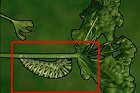
\includegraphics[height=1.75cm]{pictures/bsds500/gt/contours/marked/35028-0}\phantomsubcaption\label{subfig:datasets-bsds500}%
		\end{subfigure}
		\begin{subfigure}[t]{0.425\textwidth}%
			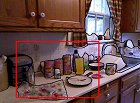
\includegraphics[height=1.75cm]{pictures/nyuv2/gt/contours/marked/00000561}\phantomsubcaption\label{subfig:datasets-nyuv2}%
		\end{subfigure}
		\\[4px]
		\begin{subfigure}[t]{0.5\textwidth}%
			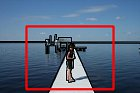
\includegraphics[height=1.75cm]{pictures/sbd/gt/contours/marked/0004774}\phantomsubcaption\label{subfig:datasets-sbd}%
		\end{subfigure}
		\begin{subfigure}[t]{0.425\textwidth}%
			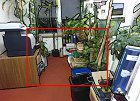
\includegraphics[height=1.75cm]{pictures/sunrgbd/gt/contours/marked/00004732}\phantomsubcaption\label{subfig:datasets-sunrgbd}%
		\end{subfigure}
	\end{subfigure}
	\hskip -3px
	\begin{subfigure}[t]{0.12\textwidth}%
		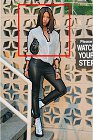
\includegraphics[height=3.68cm]{pictures/fash/gt/contours/marked/010}\phantomsubcaption\label{subfig:datasets-fash}%
	\end{subfigure}
	\caption{Example images from the used datasets. From left to right: \BSDS, \SBD, \NYU, \SUNRGBD,
	and \Fash. Black contours represent ground truth and red
	rectangles indicate excerpts used for qualitative comparison in Figures \ref{fig:experiments-qualitative-bsds500-sbd-fash} and \ref{fig:experiments-qualitative-nyuv2-sunrgbd}.
	\textbf{Best viewed in color.}}
	\label{fig:datasets}
\end{figure}

{\SUNRGBD \cite{SongLichtenbergXiao:2015}.} The Sun RGB-D dataset (\SUNRGBD)
contains $10335$ images including pre-processed depth. The dataset combines images
from the \NYU dataset and other datasets \cite{JanochKarayevJiaBarronFritzSaenkoDarrell:2011, XiaoOwensTorralba:2013}
with newly acquired images. In contrast to the \NYU dataset, the \SUNRGBD dataset combines images
from the following devices: Intel RealSense, Asus Xtion and Microsoft Kinect v1 and v2
-- we refer to \cite{SongLichtenbergXiao:2015} for details. We removed the images
taken from the \NYU dataset. The images show cluttered indoor scenes with bad lighting taken
from private apartments as well as commercial accomodations. The provided semantic
ground truth has been pre-processed similarly to the \NYU dataset.

\begin{table}[t]
    \centering
    {\scriptsize
        \begin{tabular}{r | r | c c c c c}
            && \BSDS & \SBD & \NYU & \SUNRGBD & \Fash\\\hline
            \multirow{2}{*}{\rot{Images}} & Train & 100 & 238 & 199 & 200 & 222\\
            & Test & 200 & 477 & 399 & 400 & 463\\\hline
            \multirow{2}{*}{\rot{Size}} & Train & $481 \times 321$ & $316 \times 240$ & $608 \times 448$ & $658 \times 486$ & $400 \times 600$\\
            & Test & $481 \times 321$ & $314 \times 242$ & $608 \times 448$ & $660 \times 488$ & $400 \times 600$\\\hline
    %        Ground Truth & Semantic & -- & \checkmark$^3$ & \checkmark & \checkmark & \checkmark\\
    %        & Connected Components & -- & \checkmark & -- & \checkmark & \checkmark\\
    %        & Thinning & -- & -- & \checkmark & \checkmark & --\\
    %        & Per Image & $\geq5$ & $1$ & $1$ & $1$ & $1$\\\hline
        \end{tabular}
    }
    \caption{Basic statistics of the used datasets: the total number of images,
	the number of training and test images and the size of the images (averaged per dimension).
	The number of images for the \SUNRGBD dataset excludes the images from the \NYU dataset.
	For the \NYU and \SUNRGBD datasets, training and test images have been chosen
	uniformly at random if necessary. Note that the odd numbers used for the \NYU dataset are for no
	special reason.}
    \label{table:datasets}
\end{table}

{\Fash \cite{YamaguchiKiapourOrtizBerg:2012}.} The Fashionista dataset (\Fash)
contains $685$ images which have previously been used for clothes parsing. The
images show the full body of fashion bloggers in front of various backgrounds.
Yamaguchi et al. leveraged Amazon Mechanical Turk to acquire semantic ground truth based on
pre-computed segments (\cite{YamaguchiKiapourOrtizBerg:2012} suggests that the
algorithm in \cite{ArbelaezMaireFowlkesMalik:2011} has been used). The ground truth has been
pre-processed to ensure connected segments.

\section{Benchmark}
\label{sec:benchmark}

Our benchmark aims to score the requirements for superpixels discussed in
Section \ref{sec:introduction}; in particular boundary adherence and compactness
(note that connectivity is enforced during parameter optimization, see Section \ref{subsec:parameter-optimization-connectivity}).
As these metrics inherently depend on the number of generated superpixels, we
further extend these metrics to allow the assessment of superpixel algorithms independent
of the number of generated superpixels. Therefore, let $S = \{S_j\}_{j = 1}^\K$ and 
$G = \{G_i\}$ be partitions of the same image $I: x_n \mapsto I(x_n)$, $ 1\leq n \leq N$, where 
$S$ represents a superpixel segmentation and $G$ a ground truth segmentation.

Boundary \underline{Rec}all (\Rec) \cite{MartinFowlkesMalik:2004} is the most commonly used
metric to asses boundary adherence given ground truth. Let $\text{FN}(G, S)$ and $\text{TP}(G,S)$
be the number of false negative and true positive boundary pixels in $S$
with respect to $G$. Then \Rec is defined as
\vskip -6px
\begin{align}
    \Rec(G, S) = \frac{\text{TP}(G, S)}{\text{TP}(G, S) + \text{FN}(G, S)}.
\end{align}
\vskip -4px
Overall, high \Rec represents better boundary adherence with respect to to the ground truth boundaries, \ie higher is better.
In practice, a boundary pixel in $S$ is matched to an arbitrary boundary pixel
in $G$ within a local neighborhood of size $(2r + 1) \times (2r + 1)$, with $r$ being $0.0025$ times the image diagonal
rounded to the next integer (e.g. $r = 1$ for the \BSDS dataset).

\underline{U}ndersegmentation \underline{E}rror (\UE) \cite{LevinshteinStereKutulakosFleetDickinsonSiddiqi:2009, AchantaShajiSmithLucchiFuaSuesstrunk:2012, NeubertProtzel:2012} measures the ``leakage'' of superpixels with respect to $G$ and, therefore, implicitly also measures boundary adherence.
Here, ``leakage'' refers to the overlap of superpixels with multiple, nearby ground truth segments. The original formulation by Levinshtein \etal \cite{LevinshteinStereKutulakosFleetDickinsonSiddiqi:2009} can be written as
\vskip -6px
\begin{align}
    \UEL(G, S) = \frac{1}{|G|} \sum_{G_i} \frac{\left(\sum_{S_j \cap G_i \neq \emptyset} |S_j|\right) - |G_i|}{|G_i|}\label{eq:benchmark-ue-levin}
\end{align}
\vskip -4px
where the inner term represents the ``leakage'' of superpixel $S_j$ with respect to $G$. However, some authors \cite{AchantaShajiSmithLucchiFuaSuesstrunk:2012, NeubertProtzel:2012} argue that Equation \eqref{eq:benchmark-ue-levin} penalizes superpixels overlapping only slightly with neighboring ground truth segments and is not constrained to lie in $[0, 1]$. Achanta \etal \cite{AchantaShajiSmithLucchiFuaSuesstrunk:2012} suggest to threshold the ``leakage'' term of Equation \eqref{eq:benchmark-ue-levin} and only consider those superpixels $S_j$ with a minimum overlap of $\frac{5}{100}\cdot|S_j|$. Both van den Bergh et al. \cite{VanDenBerghBoixRoigVanGool:2013} and Neubert and Protzel \cite{NeubertProtzel:2012} propose formulations not suffering from the above drawbacks. In the former,
\vskip -6px
\begin{align}
	\UEB(G, S) = \frac{1}{N} \sum_{S_j} |S_j - \arg \max_{G_i} |S_j \cap G_i||,
\end{align}
\vskip -4px
each superpixel is assigned to the ground truth segment with the largest overlap, and only the ``leakage'' with respect to other
ground truth segments is considered. Therefore, \UEB corresponds to $(1 - \ASA)$ -- with \ASA being Achievable Segmentation Accuracy as described below.
The latter,
\vskip -6px
\begin{align}
    \hspace{-0.25cm}\UENP(G, S) = \frac{1}{N} \sum_{G_i} \sum_{S_j \cap G_i \neq \emptyset} \hspace{-0.225cm} \min\{|S_j \cap G_i|, |S_j - G_i|\},
\label{eq:benchmark-ue-np}
\end{align}
\vskip -4px
is not directly equivalent to $(1 - \ASA)$, however, \UENP and \ASA are still strongly correlated as we will see later.
All formulations have in common that lower \UE refers to less ``leakage'' with respect to the ground truth, \ie lower is better.
In the following we use $\UE \equiv \UENP$.

\underline{E}xplained \underline{V}ariation (\EV) \cite{MoorePrinceWarrellMohammedJones:2008} quantifies the
quality of a superpixel segmentation without relying on ground truth.
As image boundaries tend to exhibit strong change in color and structure, \EV
assesses boundary adherence independent of human annotions. \EV is defined as
\vskip -6px
\begin{align}
    \EV(S) = \frac{\sum_{S_j} |S_j| (\mu(S_j) - \mu(I))^2}{\sum_{x_n} (I(x_n) - \mu(I))^2}
\end{align}
\vskip -4px
where $\mu(S_j)$ and $\mu(I)$ are the mean color of superpixel $S_j$ and the image $I$,
respectively. As result, \EV quantifies the variation of the image explained by the superpixels,
\ie higher is better.

\underline{Co}mpactness (\CO) \cite{SchickFischerStiefelhagen:2012} has been introduced
by Schick \etal \cite{SchickFischerStiefelhagen:2012} to evaluate the compactness of superpixels:
\vskip -6px
\begin{align}
    \CO(G, S) = \frac{1}{N} \sum_{S_j} |S_j| \frac{4\pi A(S_j)}{P(S_j)}.\label{eq:co}
\end{align}
\vskip -4px
\CO compares the area $A(S_j)$ of each superpixel $S_j$ with the
area of a circle (the most compact 2-dimensional shape) with same perimeter $P(S_j)$,
\ie higher is better.

While we will focus on \Rec, \UE, \EV and \CO, further notable metrics are briefly discussed in the following.
\underline{A}chievable \underline{S}egmentation \underline{A}ccuracy (\ASA) \cite{LiuTuzelRamalingamChellappa:2011}
quantifies the achievable accuracy for segmentation using superpixels as pre-processing step:
\vskip -6px
\begin{align}
    \ASA(G, S) = \frac{1}{N} \sum_{S_j} \max_{G_i}\{|S_j \cap G_i|\}\label{eq:benchmark-asa};
\end{align}
\vskip -4px
\underline{I}ntra-\underline{C}luster \underline{V}ariation (\ICV) \cite{BenesovaKottman:2014} computes the average variation within each superpixel:
\vskip -6px
\begin{align}
    \ICV(S) = \frac{1}{|S|} \sum_{S_j} \frac{\sqrt{\sum_{x_n \in S_j} (I(x_n) - \mu(S_j))^2}}{|S_j|};\label{eq:icv}
\end{align}
\vskip -4px
\underline{M}ean \underline{D}istance to \underline{E}dge (\MDE) \cite{BenesovaKottman:2014} refines \Rec by also considering
the distance to the nearest boundary pixel within the ground truth segmentation:
\vskip -6px
\begin{align}
    \MDE(G, S) = \frac{1}{N} \sum_{x_n \in B(G)} \text{dist}_{S}(x_n)
\end{align}
\vskip -4px
where $B(G)$ is the set of boundary pixels in $G$, and $\text{dist}_S$ is a distance transform of $S$.

\subsection{Expressiveness and Chosen Metrics}
\label{subsec:benchmark-correlation}

Due to the large number of available metrics, we examined their expressiveness
in order to systematically concentrate
on few relevant metrics. We found that \UE tends to correlate
strongly with \ASA which can be explained by Equations \eqref{eq:benchmark-ue-np}
and \eqref{eq:benchmark-asa}, respectively. In particular, simple calculation shows that
\ASA strongly resembles $(1 - \UE)$. Surprisingly, \UENP does not correlate
with \UEL suggesting that either both metrics reflect different aspects of superpixels,
or \UEL unfairly penalizes some superpixels as suggested in
\cite{AchantaShajiSmithLucchiFuaSuesstrunk:2012} and \cite{NeubertProtzel:2012}.
Unsurprisingly, \MDE correlates strongly with \Rec which can also be explained by
their respective definitions. In this sense, \MDE does not provide additional information.
Finally, \ICV does not correlate with \EV which may be attributed to the missing
normalization in Equation \eqref{eq:icv} when compared to \EV. This also results in
\ICV not begin comparable across images as the intra-cluster variation is not related to the overall
variation within the image. As of these considerations,
we concentrate on \Rec, \UE and \EV for the presented experiments. 
Details can be found in \ref{subsec:appendix-benchmark-expressiveness}.

\subsection{\AvgRec, \AvgUE and \AvgEV}
\label{subsec:benchmark-average}

As the chosen metrics inherently depend on the number of superpixels,
we seek a way of quantifying the performance with respect to \Rec, \UE and \EV 
independent of~\K and in a single plot per dataset.
In order to summarize performance over a given interval $[\K_{\min}, \K_{\max}]$,
we consider $\MR = (1 - \Rec)$, \UE and $\UEV = (1 - \EV)$. Here, the first corresponds to the
Boundary \underline{M}iss \underline{R}ate%\footnote{
%	Boundary Recall (\Rec) essentially describes a hit rate (\ie the number of true positives 
%	over the overall number of detected boundary pixels), therefore $(1 - \Rec)$ 
%	corresponds to the Boundary Miss Rate (\MR) (\ie the number of false negatives over
%	the overall number of boundary pixels).
%}
(\MR) and the last, \underline{U}nexplained \underline{V}ariation (\UEV), 
quantifies the variation in the image not explained by the superpixels.
We use the area below these curves in $[\K_{\min}, \K_{\max}] = [200, 5200]$ 
to quantify performance independent of \K. In Section \ref{subsec:experiments-quantitative}, 
we will see that these metrics appropriately summarize the performance of superpixel algorithms.
We denote these metrics by \uAvgRec (\ARec), \uAvgUE (\AUE) and
\uAvgEV (\AEV) -- note that this refers to an average over \K.
By construction (and in contrast to \Rec and \EV), lower \ARec, \AUE and \AEV is better,
making side-by-side comparison across datasets easy.

\section{Parameter Optimization}
\label{sec:parameter-optimization}

For the sake of fair comparison, we optimized parameters on the training sets depicted in Table \ref{table:datasets}.
Unfortunately, parameter optimization is not explicitly discussed in related work (\eg \cite{SchickFischerStiefelhagen:2012, AchantaShajiSmithLucchiFuaSuesstrunk:2012, NeubertProtzel:2012, SchickFischerStiefelhagen:2012})
and used parameters are not reported in most publications. In addition, varying runtimes as well as
categorical and integer parameters render parameter optimization difficult such that
we had to rely on discrete grid search, jointly optimizing \Rec and \UE, \ie minimizing $(1 - \Rec) + \UE$.
As \Rec and \UE operate on different representations (boundary pixels and superpixel segmentations, respectively),
the additive formulation ensures that algorithms balance both metrics. For example, we observed 
that using a multiplicative formulation allows superpixel algorithms to drive $(1 - \Rec)$ towards zero while disregarding \UE.
We optimized parameters for $\K \in \{400, 1200, 3600\}$ and interpolated linearly in between (however,
we found that for many algorithms, parameters are consistent across different values of $\K$).
Optimized parameters also include compactness parameters and the number of iterations
as well as the color space. We made sure that all algorithms at least support RGB color space for fairness.
In the following, we briefly discuss the main difficulties encountered during parameter optimization, namely controlling the number
of generated superpixels and ensuring connectivity.

\subsection{Controlling the Number of Generated Superpixels}
\label{subsec:parameter-optimization-superpixels}

As discussed in Section \ref{sec:introduction}, superpixel algorithms are expected
to offer control over the number of generated superpixels. We further expect the
algorithms to meet the desired number of superpixels within acceptable bounds. For
several algorithms, however, the number of generated superpixels is strongly dependent
on other parameters. Figure \ref{fig:parameter-optimization-superpixels} demonstrates the
influence of specific parameters on the number of generated superpixels
(before ensuring connectivity as in Section \ref{subsec:parameter-optimization-connectivity})
for \LSCr, \CISr, \VCr, \CRSr and \PBr. For some of the algorithms, such parameters needed to be constrained
to an appropriate value range even after enforcing connectivity.

For oversegmentation algorithms such as \FH, \EAMS and \QS not providing control
over the number of generated superpixels, we attempted to exploit simple relationships
between the provided parameters and the number of generated superpixels. For \EAMS
and \QS this allows to control the number of generated superpixels at least roughly.
\FH, in contrast, does not allow to control the number of generated superpixels
as easily. Therefore, we evaluated \FH for a large set of parameter combinations
and chose the parameters resulting in approximately the desired number of superpixels.

\FloatBarrier
\begin{figure}
	\centering
	%%%%%%%%%%%%%%%%%%%%%%%%%%%%%%%%%%%%%%%%%%%%%%%%%%%%%%%%%%%%%%%%%%%%%%%%%%%%
% Superpixels
%%%%%%%%%%%%%%%%%%%%%%%%%%%%%%%%%%%%%%%%%%%%%%%%%%%%%%%%%%%%%%%%%%%%%%%%%%%%
\begin{subfigure}[b]{\halftwoone\textwidth}
    \begin{tikzpicture}
        % CIS %%%%%%%%%%%%%%%%%%%%%%%%%%%%%%%%%%%%%%%%%%%%%%%%%%%%%%%%%%%%%%
        \begin{axis}[
                POsuperpixelsSP,
                xmin=1,xmax=10,
                xtick=\empty,
                ylabel=\K,
                xlabel=parameter,
                title=\BSDS,
                title style={xshift=2cm}]

            \addplot[CIS,transparent] coordinates{
                (1,9887.95)
                (3,2321)
                (5,1022.8)
                (7,652.94)
                (10,468.2)
            };
        \end{axis}
        \begin{axis}[
                POsuperpixelsSP,
                xmin=1,xmax=10,
                axis y line=none,
                axis x line=none,
                xlabel=none,
                ylabel=none]

            \addplot[CIS] coordinates{
                (1,9887.95)
                (3,2321)
                (5,1022.8)
                (7,652.94)
                (10,468.2)
            };
            \label{plot:parameter-optimization-superpixels-cis}
        \end{axis}

        % CRS %%%%%%%%%%%%%%%%%%%%%%%%%%%%%%%%%%%%%%%%%%%%%%%%%%%%%%%%%%%%%%
        \begin{axis}[
                POsuperpixelsSP,
                xmin=0.001,xmax=0.1,
                axis y line=none,
                axis x line=none,
                xlabel=none,
                ylabel=none,]

            \addplot[CRS] coordinates{
                (0.001,10314.1)
                (0.005,6844.61)
                (0.01,4712.74)
                (0.05,1060.46)
                (0.1,609.12)
            };
            \label{plot:parameter-optimization-superpixels-crs}
        \end{axis}

        % PB %%%%%%%%%%%%%%%%%%%%%%%%%%%%%%%%%%%%%%%%%%%%%%%%%%%%%%%%%%%%%%%
        \begin{axis}[
                POsuperpixelsSP,
                xmin=1,xmax=20,
                axis y line=none,
                axis x line=none,
                xlabel=none,
                ylabel=none]

            \addplot[PB] coordinates{
                (1,5933.48)
                (2.5,3532.01)
                (5,2012.83)
                (7.5,1382.84)
                (10,1057.3)
                (20,608.12)
            };
            \label{plot:parameter-optimization-superpixels-pb}
        \end{axis}

        % LSC %%%%%%%%%%%%%%%%%%%%%%%%%%%%%%%%%%%%%%%%%%%%%%%%%%%%%%%%%%%%%%
        \begin{axis}[
                POsuperpixelsSP,
                xmin=0,xmax=0.5,
                axis y line=none,
                axis x line=none,
                xlabel=none,
                ylabel=none]

            \addplot[LSC] coordinates{
                (0,2616.8)
                (0.01,2581.57)
                (0.05,2218.48)
                (0.1,1743.55)
                (0.25,880.76)
                (0.5,488.51)
            };
            \label{plot:parameter-optimization-superpixels-lsc}
        \end{axis}

        % VC %%%%%%%%%%%%%%%%%%%%%%%%%%%%%%%%%%%%%%%%%%%%%%%%%%%%%%%%%%%%%%%
        \begin{axis}[
                POsuperpixelsSP,
                xmin=10,xmax=250,
                axis y line=none,
                axis x line=none,
                xlabel=none,
                ylabel=none]

            \addplot[VC] coordinates{
                (10,13548.4)
                (25,6936.92)
                (50,3539.36)
                (100,1651.79)
                (250,662.58)
            };
            \label{plot:parameter-optimization-superpixels-vc}
        \end{axis}
    \end{tikzpicture}
\end{subfigure}
\begin{subfigure}[b]{\halftwoone\textwidth}
    \begin{tikzpicture}
        % CIS %%%%%%%%%%%%%%%%%%%%%%%%%%%%%%%%%%%%%%%%%%%%%%%%%%%%%%%%%%%%%%
        \begin{axis}[
                POsuperpixelsRec,
                xmin=1,xmax=10,
                xtick=\empty,
                ylabel=\Rec,
                xlabel=parameter]

            \addplot[CIS,transparent] coordinates{
                (1,0.891961)
                (3,0.807977)
                (5,0.755691)
                (7,0.726976)
                (10,0.69987)
            };
        \end{axis}
        \begin{axis}[
                POsuperpixelsRec,
                xmin=1,xmax=10,
                axis y line=none,
                axis x line=none,
                xlabel=none,
                ylabel=none]

            \addplot[CIS] coordinates{
                (1,0.891961)
                (3,0.807977)
                (5,0.755691)
                (7,0.726976)
                (10,0.69987)
            };
            \label{plot:parameter-optimization-superpixels-cis}
        \end{axis}

        % CRS %%%%%%%%%%%%%%%%%%%%%%%%%%%%%%%%%%%%%%%%%%%%%%%%%%%%%%%%%%%%%%
        \begin{axis}[
                POsuperpixelsRec,
                xmin=0.001,xmax=0.1,
                axis y line=none,
                axis x line=none,
                xlabel=none,
                ylabel=none,]

            \addplot[CRS] coordinates{
                (0.001,0.965601)
                (0.005,0.938007)
                (0.01,0.900849)
                (0.05,0.671317)
                (0.1,0.564656)
            };
            \label{plot:parameter-optimization-superpixels-crs}
        \end{axis}

        % PB %%%%%%%%%%%%%%%%%%%%%%%%%%%%%%%%%%%%%%%%%%%%%%%%%%%%%%%%%%%%%%%
        \begin{axis}[
                POsuperpixelsRec,
                xmin=1,xmax=20,
                axis y line=none,
                axis x line=none,
                xlabel=none,
                ylabel=none]

            \addplot[PB] coordinates{
                (1,0.970505)
                (2.5,0.917979)
                (5,0.840081)
                (7.5,0.783602)
                (10,0.744347)
                (20,0.677509)
            };
            \label{plot:parameter-optimization-superpixels-pb}
        \end{axis}

        % LSC %%%%%%%%%%%%%%%%%%%%%%%%%%%%%%%%%%%%%%%%%%%%%%%%%%%%%%%%%%%%%%
        \begin{axis}[
                POsuperpixelsRec,
                xmin=0,xmax=0.5,
                axis y line=none,
                axis x line=none,
                xlabel=none,
                ylabel=none]

            \addplot[LSC] coordinates{
                (0,0.89937)
                (0.01,0.898078)
                (0.05,0.884433)
                (0.1,0.853266)
                (0.25,0.747625)
                (0.5,0.61054)
            };
            \label{plot:parameter-optimization-superpixels-lsc}
        \end{axis}

        % VC %%%%%%%%%%%%%%%%%%%%%%%%%%%%%%%%%%%%%%%%%%%%%%%%%%%%%%%%%%%%%%%
        \begin{axis}[
                POsuperpixelsRec,
                xmin=10,xmax=250,
                axis y line=none,
                axis x line=none,
                xlabel=none,
                ylabel=none]

            \addplot[VC] coordinates{
                (10,0.939249)
                (25,0.893879)
                (50,0.842431)
                (100,0.784252)
                (250,0.700503)
            };
            \label{plot:parameter-optimization-superpixels-vc}
        \end{axis}
    \end{tikzpicture}
\end{subfigure}

	\caption{\K and \Rec on the training set of the \BSDS dataset when varying
	parameters strongly influencing the number of generated superpixels
	of: \LSCr; \CISr; \VCr; \CRSr; and \PBr.
	The parameters have been omitted and scaled for clarity.
	A higher number of superpixels results in increased \Rec. Therefore, unnoticed
	superpixels inherently complicate fair comparison.
	\textbf{Best viewed in color.}
	}
	\label{fig:parameter-optimization-superpixels}
\end{figure}
\begin{figure}
	\centering
    %%%%%%%%%%%%%%%%%%%%%%%%%%%%%%%%%%%%%%%%%%%%%%%%%%%%%%%%%%%%%%%%%%%%%%%%%%%%
% Iterations
%%%%%%%%%%%%%%%%%%%%%%%%%%%%%%%%%%%%%%%%%%%%%%%%%%%%%%%%%%%%%%%%%%%%%%%%%%%%
\begin{subfigure}[b]{\halftwoone\textwidth}
    \begin{tikzpicture}
        % CIS %%%%%%%%%%%%%%%%%%%%%%%%%%%%%%%%%%%%%%%%%%%%%%%%%%%%%%%%%%%%%%
        \begin{axis}[
                POiterationsRec,
                xmin=1,xmax=25,
                yshift=-0cm,
                xtick={1,3,5,10,25},
                ylabel=\Rec,
                xlabel=iterations,
                title=\BSDS,
                title style={xshift=2cm}]

            \addplot[CIS,transparent] coordinates{
                (1,0.729313)
                (3,0.69987)
            };
        \end{axis}
        %\begin{axis}[
        %        POiterationsRec,
        %        xmin=1,xmax=25,
        %        axis y line=none,
        %        axis x line=none,
        %        xlabel=none,
        %        ylabel=none]
        %
        %    \addplot[CIS] coordinates{
        %        (1,0.729313)
        %        (3,0.69987)
        %    };
        %    \label{plot:parameter-optimization-iterations-cis}
        %\end{axis}

        % SLIC %%%%%%%%%%%%%%%%%%%%%%%%%%%%%%%%%%%%%%%%%%%%%%%%%%%%%%%%%%%%%
        \begin{axis}[
                POiterationsRec,
                xmin=1,xmax=25,
                axis y line=none,
                axis x line=none,
                xlabel=none,
                ylabel=none]

            \addplot[SLIC] coordinates{
                (1,0.747771)
                (5,0.766599)
                (10,0.770892)
                (25,0.774302)
                (50,0.773565)
            };
            \label{plot:parameter-optimization-iterations-preslic}
        \end{axis}

        % preSLIC %%%%%%%%%%%%%%%%%%%%%%%%%%%%%%%%%%%%%%%%%%%%%%%%%%%%%%%%%%
        \begin{axis}[
                POiterationsRec,
                xmin=1,xmax=25,
                axis y line=none,
                axis x line=none,
                xlabel=none,
                ylabel=none]

            \addplot[preSLIC] coordinates{
                (1,0.736228)
                (5,0.742702)
                (10,0.742702)
                (25,0.742702)
                (50,0.742702)
            };
            \label{plot:parameter-optimization-iterations-preslic}
        \end{axis}

        % LSC %%%%%%%%%%%%%%%%%%%%%%%%%%%%%%%%%%%%%%%%%%%%%%%%%%%%%%%%%%%%%%
        \begin{axis}[
                POiterationsRec,
                xmin=1,xmax=25,
                axis y line=none,
                axis x line=none,
                xlabel=none,
                ylabel=none]

            \addplot[LSC] coordinates{
                (1,0.888483)
                (5,0.89937)
                (10,0.898183)
                (25,0.896311)
                (50,0.895474)
            };
            \label{plot:parameter-optimization-iterations-lsc}
        \end{axis}

        % CRS %%%%%%%%%%%%%%%%%%%%%%%%%%%%%%%%%%%%%%%%%%%%%%%%%%%%%%%%%%%%%%
        \begin{axis}[
                POiterationsRec,
                xmin=1,xmax=25,
                axis y line=none,
                axis x line=none,
                xlabel=none,
                ylabel=none]

            \addplot[CRS] coordinates{
                (1,0.861408)
                (3,0.873871)
                (6,0.874965)
            };
            \label{plot:parameter-optimization-iterations-crs}
        \end{axis}

        % SEEDS %%%%%%%%%%%%%%%%%%%%%%%%%%%%%%%%%%%%%%%%%%%%%%%%%%%%%%%%%%%%
        \begin{axis}[
                POiterationsRec,
                xmin=1,xmax=25,
                axis y line=none,
                axis x line=none,
                xlabel=none,
                ylabel=none]

            \addplot[SEEDS] coordinates{
                (1,0.775507)
                (2,0.841535)
                (10,0.929071)
                (25,0.94386)
            };
            \label{plot:parameter-optimization-iterations-seeds}
        \end{axis}

        % ETPS %%%%%%%%%%%%%%%%%%%%%%%%%%%%%%%%%%%%%%%%%%%%%%%%%%%%%%%%%%%%%
        \begin{axis}[
                POiterationsRec,
                xmin=5,xmax=25,
                axis y line=none,
                axis x line=none,
                xlabel=none,
                ylabel=none]

            \addplot[ETPS] coordinates{
                (5,0.932699)
                (10,0.932985)
                (25,0.933014)
            };
            \label{plot:parameter-optimization-iterations-etps}
        \end{axis}

        % CCS %%%%%%%%%%%%%%%%%%%%%%%%%%%%%%%%%%%%%%%%%%%%%%%%%%%%%%%%%%%%%
        \begin{axis}[
                POiterationsRec,
                xmin=1,xmax=25,
                axis y line=none,
                axis x line=none,
                xlabel=none,
                ylabel=none]

            \addplot[CCS] coordinates{
                (1,0.423352)
                (5,0.637979)
                (25,0.752122)
            };
            \label{plot:parameter-optimization-iterations-ccs}
        \end{axis}
    \end{tikzpicture}
\end{subfigure}
\begin{subfigure}[b]{\halftwoone\textwidth}
    \begin{tikzpicture}
        % CIS %%%%%%%%%%%%%%%%%%%%%%%%%%%%%%%%%%%%%%%%%%%%%%%%%%%%%%%%%%%%%%
        \begin{axis}[
                POiterationst,
                xmin=1,xmax=25,
                yshift=-0cm,
                xtick={1,3,5,10,25},
                ytick={0,0.1,1,10},
                ylabel=$\log t$,
                xlabel=iterations,
                ymode=log]

            \addplot[CIS,transparent] coordinates{
                (1,2.08)
                (3,5.26)
            };
        \end{axis}
        %\begin{axis}[
        %        POiterationsRec,
        %        xmin=1,xmax=3,
        %        axis y line=none,
        %        axis x line=none,
        %        xlabel=none,
        %        ylabel=none]
        %
        %    \addplot[CIS] coordinates{
        %        (1,2.08)
        %        (3,5.26)
        %    };
        %    \label{plot:parameter-optimization-iterations-cis}
        %\end{axis}

        % SLIC %%%%%%%%%%%%%%%%%%%%%%%%%%%%%%%%%%%%%%%%%%%%%%%%%%%%%%%%%%%%%
        \begin{axis}[
                POiterationst,
                xmin=1,xmax=25,
                axis y line=none,
                axis x line=none,
                xlabel=none,
                ylabel=none,
                ymode=log]

            \addplot[SLIC] coordinates{
                (1,0.059)
                (10,0.094)
                (25,0.148)
                (50,0.242)
            };
            \label{plot:parameter-optimization-iterations-preslic}
        \end{axis}

        % preSLIC %%%%%%%%%%%%%%%%%%%%%%%%%%%%%%%%%%%%%%%%%%%%%%%%%%%%%%%%%%
        \begin{axis}[
                POiterationst,
                xmin=1,xmax=25,
                axis y line=none,
                axis x line=none,
                xlabel=none,
                ylabel=none,
                ymode=log]

            \addplot[preSLIC] coordinates{
                (1,0.013)
                (10,0.03)
                (25,0.029)
                (50,0.03)
            };
            \label{plot:parameter-optimization-iterations-preslic}
        \end{axis}

        % TODO
        % LSC %%%%%%%%%%%%%%%%%%%%%%%%%%%%%%%%%%%%%%%%%%%%%%%%%%%%%%%%%%%%%%
        \begin{axis}[
                POiterationst,
                xmin=1,xmax=25,
                axis y line=none,
                axis x line=none,
                xlabel=none,
                ylabel=none,
                ymode=log]

            \addplot[LSC] coordinates{
                (1,0.112)
                (5,0.89937)
                (10,0.898183)
                (25,0.896311)
                (50,0.895474)
            };
            \label{plot:parameter-optimization-iterations-lsc}
        \end{axis}

        % CRS %%%%%%%%%%%%%%%%%%%%%%%%%%%%%%%%%%%%%%%%%%%%%%%%%%%%%%%%%%%%%%
        \begin{axis}[
                POiterationst,
                xmin=1,xmax=25,
                axis y line=none,
                axis x line=none,
                xlabel=none,
                ylabel=none,
                ymode=log]

            \addplot[CRS] coordinates{
                (1,0.329)
                (3,1.169)
                (6,2.342)
            };
            \label{plot:parameter-optimization-iterations-crs}
        \end{axis}

        % SEEDS %%%%%%%%%%%%%%%%%%%%%%%%%%%%%%%%%%%%%%%%%%%%%%%%%%%%%%%%%%%%
        \begin{axis}[
                POiterationst,
                xmin=1,xmax=25,
                axis y line=none,
                axis x line=none,
                xlabel=none,
                ylabel=none,
                ymode=log]

            \addplot[SEEDS] coordinates{
                (1,0.026)
                (10,1.986)
                (25,4.775)
                %(50,9.421)
            };
            \label{plot:parameter-optimization-iterations-seeds}
        \end{axis}

        % ETPS %%%%%%%%%%%%%%%%%%%%%%%%%%%%%%%%%%%%%%%%%%%%%%%%%%%%%%%%%%%%%
        \begin{axis}[
                POiterationst,
                xmin=5,xmax=25,
                axis y line=none,
                axis x line=none,
                xlabel=none,
                ylabel=none,
                ymode=log]

            \addplot[ETPS] coordinates{
                (5,0.167)
                (10,0.308)
                (25,0.711)
            };
            \label{plot:parameter-optimization-iterations-etps}
        \end{axis}

        % CCS %%%%%%%%%%%%%%%%%%%%%%%%%%%%%%%%%%%%%%%%%%%%%%%%%%%%%%%%%%%%%
        \begin{axis}[
                POiterationsRec,
                xmin=1,xmax=25,
                axis y line=none,
                axis x line=none,
                xlabel=none,
                ylabel=none]

            \addplot[CCS] coordinates{
                (1,0.0665)
                (5,0.0985002)
                (25,0.14135)
            };
            \label{plot:parameter-optimization-iterations-ccs}
        \end{axis}
    \end{tikzpicture}
\end{subfigure}

    \caption{\Rec and runtime in seconds $t$ on the training set of the \BSDS dataset
	when varying the number of iterations of: \SLICr; \CRSr; \SEEDSr; \preSLICr; \LSCr; and \ETPSr.
	Most algorithms achieve reasonable \Rec with about $3 - 10$ iterations. Still,
	parameter optimization with respect to \Rec and \UE favors more iterations.
	\textbf{Best viewed in color.}}
    \label{fig:parameter-optimization-iterations}
\end{figure}
\begin{figure}
	\centering
    %%%%%%%%%%%%%%%%%%%%%%%%%%%%%%%%%%%%%%%%%%%%%%%%%%%%%%%%%%%%%%%%%%%%%%%%%%%%
% Compactness
%%%%%%%%%%%%%%%%%%%%%%%%%%%%%%%%%%%%%%%%%%%%%%%%%%%%%%%%%%%%%%%%%%%%%%%%%%%%
\begin{subfigure}[b]{\halftwoone\textwidth}\phantomsubcaption\label{subfig:parameter-optimization-compactness-rec}
    \begin{tikzpicture}
        % SLIC %%%%%%%%%%%%%%%%%%%%%%%%%%%%%%%%%%%%%%%%%%%%%%%%%%%%%%%%%%%%%
        \begin{axis}[
                POcompactnessRec,
                xmin=1,xmax=160,
                xtick=\empty,
                yshift=-0cm,
                ylabel=\Rec,
                xlabel=compactness,
                title=\BSDS,
                title style={xshift=2cm}]

            \addplot[SLIC,transparent] coordinates{
                (1,0.695708)
                (5,0.698356)
                (10,0.708017)
                (20,0.726845)
                (40,0.743767)
                (80,0.718759)
                (160,0.628553)
            };
        \end{axis}
        \begin{axis}[
                POcompactnessRec,
                xmin=1,xmax=160,
                axis y line=none,
                axis x line=none,
                xlabel=none,
                ylabel=none]

            \addplot[SLIC] coordinates{
                (1,0.695708)
                (5,0.698356)
                (10,0.708017)
                (20,0.726845)
                (40,0.743767)
                (80,0.718759)
                (160,0.628553)
            };
            \label{plot:parameter-optimization-iterations-slic}
        \end{axis}

        % CRS %%%%%%%%%%%%%%%%%%%%%%%%%%%%%%%%%%%%%%%%%%%%%%%%%%%%%%%%%%%%%%
        \begin{axis}[
                POcompactnessRec,
                xmin=0,xmax=0.1,
                axis y line=none,
                axis x line=none,
                xlabel=none,
                ylabel=none]

            \addplot[CRS] coordinates{
                (0.001,0.965601)
                (0.005,0.938007)
                (0.01,0.900849)
                (0.05,0.671317)
                (0.1,0.564656)
            };
            \label{plot:parameter-optimization-iterations-crs}
        \end{axis}

        % reSEEDS %%%%%%%%%%%%%%%%%%%%%%%%%%%%%%%%%%%%%%%%%%%%%%%%%%%%%%%%%%
        %\begin{axis}[
        %        POcompactnessRec,
        %        xmin=0,xmax=0.5,
        %        axis y line=none,
        %        axis x line=none,
        %        xlabel=none,
        %        ylabel=none]
        %
        %    \addplot[reSEEDS] coordinates{
        %        (0,0.941375)
        %        (0.25,0.911667)
        %        (0.5,0.886816)
        %    };
        %    \label{plot:parameter-optimization-iterations-reseeds}
        %\end{axis}

        % VC %%%%%%%%%%%%%%%%%%%%%%%%%%%%%%%%%%%%%%%%%%%%%%%%%%%%%%%%%%%%%%%
        \begin{axis}[
                POcompactnessRec,
                xmin=10,xmax=250,
                axis y line=none,
                axis x line=none,
                xlabel=none,
                ylabel=none]

            \addplot[VC] coordinates{
                (10,0.939249)
                (25,0.893879)
                (50,0.842431)
                (100,0.784252)
                (250,0.700503)
            };
            \label{plot:parameter-optimization-iterations-vc}
        \end{axis}

        % CW %%%%%%%%%%%%%%%%%%%%%%%%%%%%%%%%%%%%%%%%%%%%%%%%%%%%%%%%%%%%%%%
        \begin{axis}[
                POcompactnessRec,
                xmin=0,xmax=10,
                axis y line=none,
                axis x line=none,
                xlabel=none,
                ylabel=none]

            \addplot[CW] coordinates{
                (0.01,0.742971)
                (0.05,0.747513)
                (0.1,0.746982)
                (0.5,0.719384)
                (1,0.690183)
                (5,0.551541)
                (10,0.48157)
            };
            \label{plot:parameter-optimization-iterations-cw}
        \end{axis}

        % preSLIC %%%%%%%%%%%%%%%%%%%%%%%%%%%%%%%%%%%%%%%%%%%%%%%%%%%%%%%%%%
        \begin{axis}[
                POcompactnessRec,
                xmin=1,xmax=160,
                axis y line=none,
                axis x line=none,
                xlabel=none,
                ylabel=none]

            \addplot[preSLIC] coordinates{
                (1,0.7024)
                (5,0.719238)
                (10,0.735199)
                (20,0.742702)
                (40,0.719054)
                (80,0.626927)
                (160,0.494195)
            };
            \label{plot:parameter-optimization-iterations-preslic}
        \end{axis}

        % ERGC %%%%%%%%%%%%%%%%%%%%%%%%%%%%%%%%%%%%%%%%%%%%%%%%%%%%%%%%%%%%%
        \begin{axis}[
                POcompactnessRec,
                xmin=0,xmax=25,
                axis y line=none,
                axis x line=none,
                xlabel=none,
                ylabel=none]

            \addplot[ERGC] coordinates{
                (0,0.793333)
                (1,0.790007)
                (2,0.787139)
                (5,0.779947)
                (10,0.770237)
                (25,0.749098)
            };
            \label{plot:parameter-optimization-iterations-ergc}
        \end{axis}

        % LSC %%%%%%%%%%%%%%%%%%%%%%%%%%%%%%%%%%%%%%%%%%%%%%%%%%%%%%%%%%%%%%
        \begin{axis}[
                POcompactnessRec,
                xmin=0,xmax=0.5,
                axis y line=none,
                axis x line=none,
                xlabel=none,
                ylabel=none]

            \addplot[LSC] coordinates{
                (0,0.89937)
                (0.01,0.898078)
                (0.05,0.884433)
                (0.1,0.853266)
                (0.25,0.747625)
                (0.5,0.61054)
            };
            \label{plot:parameter-optimization-iterations-lsc}
        \end{axis}

        % ETPS %%%%%%%%%%%%%%%%%%%%%%%%%%%%%%%%%%%%%%%%%%%%%%%%%%%%%%%%%%%%%
        \begin{axis}[
                POcompactnessRec,
                xmin=0,xmax=10,
                axis y line=none,
                axis x line=none,
                xlabel=none,
                ylabel=none]

            \addplot[ETPS] coordinates{
                (0.01,0.933014)
                (0.05,0.91386)
                (0.1,0.898893)
                (0.5,0.832607)
                (1,0.789218)
                (5,0.661253)
                (10,0.601947)
            };
            \label{plot:parameter-optimization-iterations-etps}
        \end{axis}

        % CCS %%%%%%%%%%%%%%%%%%%%%%%%%%%%%%%%%%%%%%%%%%%%%%%%%%%%%%%%%%%%%
        \begin{axis}[
                POcompactnessRec,
                xmin=25,xmax=500,
                axis y line=none,
                axis x line=none,
                xlabel=none,
                ylabel=none]

            \addplot[CCS] coordinates{
               	(25,0.845181)
               	(50,0.81119)
               	(100,0.76329)
               	(250,0.668066)
               	(500,0.578618)
            };
            \label{plot:parameter-optimization-iterations-ccs}
        \end{axis}
    \end{tikzpicture}
\end{subfigure}
\begin{subfigure}[b]{\halftwoone\textwidth}\phantomsubcaption\label{subfig:parameter-optimization-compactness-co}
    \begin{tikzpicture}
        % SLIC %%%%%%%%%%%%%%%%%%%%%%%%%%%%%%%%%%%%%%%%%%%%%%%%%%%%%%%%%%%%%
        \begin{axis}[
                POcompactnessCO,
                xmin=1,xmax=160,
                xtick=\empty,
                yshift=-0cm,
                %xlabel=\ref{plot:parameter-optimization-iterations-slic},
                ylabel=\CO,
                xlabel=compactness]

            \addplot[SLIC,transparent] coordinates{
                (1,0.18298)
                (5,0.189713)
                (10,0.205343)
                (20,0.240073)
                (40,0.298561)
                (80,0.388942)
                (160,0.503195)
            };
        \end{axis}
        \begin{axis}[
                POcompactnessCO,
                xmin=1,xmax=160,
                axis y line=none,
                axis x line=none,
                xlabel=none,
                ylabel=none]

            \addplot[SLIC] coordinates{
                (1,0.18298)
                (5,0.189713)
                (10,0.205343)
                (20,0.240073)
                (40,0.298561)
                (80,0.388942)
                (160,0.503195)
            };
            \label{plot:parameter-optimization-iterations-slic}
        \end{axis}

        % CRS %%%%%%%%%%%%%%%%%%%%%%%%%%%%%%%%%%%%%%%%%%%%%%%%%%%%%%%%%%%%%%
        \begin{axis}[
                POcompactnessCO,
                xmin=0,xmax=0.1,
                axis y line=none,
                axis x line=none,
                xlabel=none,
                ylabel=none]

            \addplot[CRS] coordinates{
                (0.001,0.189319)
                (0.005,0.168872)
                (0.01,0.171872)
                (0.05,0.34985)
                (0.1,0.470495)
            };
            \label{plot:parameter-optimization-iterations-crs}
        \end{axis}

        % reSEEDS %%%%%%%%%%%%%%%%%%%%%%%%%%%%%%%%%%%%%%%%%%%%%%%%%%%%%%%%%%
        %\begin{axis}[
        %        POcompactnessCO,
        %        xmin=0,xmax=0.5,
        %        axis y line=none,
        %        axis x line=none,
        %        xlabel=none,
        %        ylabel=none]
        %
        %    \addplot[reSEEDS] coordinates{
        %        (0,0.0588565)
        %        (0.25,0.140091)
        %        (0.5,0.187924)
        %    };
        %    \label{plot:parameter-optimization-iterations-reseeds}
        %\end{axis}

        % VC %%%%%%%%%%%%%%%%%%%%%%%%%%%%%%%%%%%%%%%%%%%%%%%%%%%%%%%%%%%%%%%
        \begin{axis}[
                POcompactnessCO,
                xmin=10,xmax=250,
                axis y line=none,
                axis x line=none,
                xlabel=none,
                ylabel=none]

            \addplot[VC] coordinates{
                (10,0.319304)
                (25,0.330338)
                (50,0.363377)
                (100,0.414478)
                (250,0.488505)
            };
            \label{plot:parameter-optimization-iterations-vc}
        \end{axis}

        % CW %%%%%%%%%%%%%%%%%%%%%%%%%%%%%%%%%%%%%%%%%%%%%%%%%%%%%%%%%%%%%%%
        \begin{axis}[
                POcompactnessCO,
                xmin=0,xmax=10,
                axis y line=none,
                axis x line=none,
                xlabel=none,
                ylabel=none]

            \addplot[CW] coordinates{
                (0.01,0.24516)
                (0.05,0.268145)
                (0.1,0.280659)
                (0.5,0.327715)
                (1,0.362302)
                (5,0.474638)
                (10,0.539703)
            };
            \label{plot:parameter-optimization-iterations-cw}
        \end{axis}

        % preSLIC %%%%%%%%%%%%%%%%%%%%%%%%%%%%%%%%%%%%%%%%%%%%%%%%%%%%%%%%%%
        \begin{axis}[
                POcompactnessCO,
                xmin=1,xmax=160,
                axis y line=none,
                axis x line=none,
                xlabel=none,
                ylabel=none]

            \addplot[preSLIC] coordinates{
                (1,0.182145)
                (5,0.202452)
                (10,0.233752)
                (20,0.286967)
                (40,0.371689)
                (80,0.494547)
                (160,0.63925)
            };
            \label{plot:parameter-optimization-iterations-preslic}
        \end{axis}

        % ERGC %%%%%%%%%%%%%%%%%%%%%%%%%%%%%%%%%%%%%%%%%%%%%%%%%%%%%%%%%%%%%
        \begin{axis}[
                POcompactnessCO,
                xmin=0,xmax=25,
                axis y line=none,
                axis x line=none,
                xlabel=none,
                ylabel=none]

            \addplot[ERGC] coordinates{
                (0,0.225633)
                (1,0.247766)
                (2,0.257937)
                (5,0.278561)
                (10,0.300108)
                (25,0.337102)
            };
            \label{plot:parameter-optimization-iterations-ergc}
        \end{axis}

        % LSC %%%%%%%%%%%%%%%%%%%%%%%%%%%%%%%%%%%%%%%%%%%%%%%%%%%%%%%%%%%%%%
        \begin{axis}[
                POcompactnessCO,
                xmin=0,xmax=0.5,
                axis y line=none,
                axis x line=none,
                xlabel=none,
                ylabel=none]

            \addplot[LSC] coordinates{
                (0,0.176833)
                (0.01,0.178685)
                (0.05,0.216972)
                (0.1,0.272364)
                (0.25,0.408945)
                (0.5,0.552146)
            };
            \label{plot:parameter-optimization-iterations-lsc}
        \end{axis}

        % ETPS %%%%%%%%%%%%%%%%%%%%%%%%%%%%%%%%%%%%%%%%%%%%%%%%%%%%%%%%%%%%%
        \begin{axis}[
                POcompactnessCO,
                xmin=0,xmax=10,
                axis y line=none,
                axis x line=none,
                xlabel=none,
                ylabel=none]

            \addplot[ETPS] coordinates{
                (0.01,0.104933)
                (0.05,0.153633)
                (0.1,0.185856)
                (0.5,0.293024)
                (1,0.351901)
                (5,0.499763)
                (10,0.551916)
            };
            \label{plot:parameter-optimization-iterations-etps}
        \end{axis}

        % CCS %%%%%%%%%%%%%%%%%%%%%%%%%%%%%%%%%%%%%%%%%%%%%%%%%%%%%%%%%%%%%
        \begin{axis}[
                POcompactnessCO,
                xmin=25,xmax=500,
                axis y line=none,
                axis x line=none,
                xlabel=none,
                ylabel=none]

            \addplot[CCS] coordinates{
                (25,0.198658)
                (50,0.249623)
                (100,0.319781)
                (250,0.431699)
                (500,0.509652)
            };
            \label{plot:parameter-optimization-iterations-ccs}
        \end{axis}
    \end{tikzpicture}
\end{subfigure}

    \caption{\Rec and \CO on the training set of the \BSDS dataset when varying the compactness parameter of:
	\SLICr; \CRSr; \VCr; \preSLICr; \CWr; \ERGCr; \LSCr; and \ETPSr.
	The parameters have been omitted and scaled for clarity.
	High \CO comes at the cost of reduced \Rec and parameter optimization
	with respect to \Rec and \UE results in less compact superpixels.
	\textbf{Best viewed in color.}}
    \label{fig:parameter-optimization-compactness}
	\vskip 12px
	% Total: 26 (+2 depth)
%\begin{mdframed}[userdefinedwidth=0.5\textwidth]
	{\scriptsize
		\def\arraystretch{0.8}
		% \LSCr; \CISr; \VCr; \CRSr; and \PBr; \SLICr; \CRSr; \SEEDSr; \preSLICr; \LSCr; and \ETPSr;
		% \SLICr; \CRSr; \VCr; \preSLICr; \CWr; \ERGCr; \LSCr; and \ETPSr; \CCSr
		\begin{tabularx}{0.475\textwidth}{X X X l}
			\ref{plot:cis} \CIS &
			\ref{plot:slic} \SLIC &
			\ref{plot:crs} \CRS &
			\ref{plot:ers} \ERS \\
			\ref{plot:pb} \PB &
			\ref{plot:seeds} \SEEDS &
			\ref{plot:vc} \VC &
			\ref{plot:ccs} \CCS \\
			\ref{plot:cw} \CW &
			\ref{plot:ergc} \ERGC &
			\ref{plot:preslic} \preSLIC &
			\ref{plot:wp} \WP \\%TODO
			\ref{plot:etps} \ETPS &
			\ref{plot:lsc} \LSC & &
		\end{tabularx}
	}
%\end{mdframed}

\end{figure}
\FloatBarrier

\subsection{Ensuring Connectivity}
\label{subsec:parameter-optimization-connectivity}

Unfortunately, many implementations (note the difference between implementation and algorithm)
cannot ensure the connectivity of the generated superpixels as required in Section \ref{sec:introduction}.
Therefore, we decided to strictly enforce connectivity using a connected components algorithm,
\ie  after computing superpixels, each connected component is relabeled as separate superpixel. For some implementations,
this results in many unintended superpixels comprising few pixels. In these cases
we additionally merge the newly generated superpixels into larger neighboring ones.
However, even with these post-processing steps, the evaluated implementations of \CIS, \CRS, \PB, \DASP, \VC, \VCCS or \LSC
generate highly varying numbers of superpixels across different images.

\subsection{Common Trade-Offs: Runtime and Compactness}
\label{subsec:parameter-optimization-trade-offs}

Two other types of parameters deserve detailed discussion: the number of iterations
and the compactness parameter. The former controls the trade-off between runtime and performance,
exemplarily demonstrated in Figure \ref{fig:parameter-optimization-iterations}
showing that more iterations usually result in higher \Rec and higher runtime in
seconds $t$. The latter controls the trade-off between compactness and performance and
Figure \ref{fig:parameter-optimization-compactness} shows that higher \CO usually
results in lower \Rec. Overall, parameter optimization with respect to \Rec and \UE
results in higher runtime and lower compactness.

\section{Experiments}
\label{sec:experiments}

Our experiments include visual quality, performance with respect to \Rec, \UE and
\EV as well as runtime. In contrast to existing work \cite{SchickFischerStiefelhagen:2012, AchantaShajiSmithLucchiFuaSuesstrunk:2012, NeubertProtzel:2012, SchickFischerStiefelhagen:2012}, we consider
minimum/maximum and standard deviation of \Rec, \UE and \EV (in relation to the number of generated superpixels \K) and present results
for the introduced metrics \ARec, \AUE and \AEV.
Furthermore, we present experiments regarding implementation details as well as robustness
against noise, blur and affine transformations. Finally, we give an overall ranking based on \ARec and \AUE.

\subsection{Qualitative}
\label{subsec:experiments-qualitative}

\def\BSDSCroppedScale{0.25}
\def\SBDCroppedScale{0.3}
\def\FashCroppedScale{0.195}
\begin{figure*}
	\centering
	\vspace{-0.5cm}
	% W %%%%%%%%%%%%%%%%%%%%%%%%%%%%%%%%%%%%%%%%%%%%%%%%%%%%%%%%%%%%%%%%%%%%%%%%
	\begin{subfigure}[b]{0.02\textwidth}
		\rotatebox{90}{\small\hphantom{aaai}\W}
	\end{subfigure}
	\begin{subfigure}[b]{0.16\textwidth}
        \begin{center}
            \BSDS
        \end{center}
        \vskip -6px
		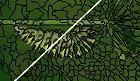
\includegraphics[height=1.65cm]{pictures/bsds500/w/cropped/w_35028_contours}
	\end{subfigure}
	\begin{subfigure}[b]{0.129\textwidth}
        \begin{center}
            \SBD
        \end{center}
        \vskip -6px
		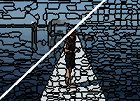
\includegraphics[height=1.65cm]{pictures/sbd/w/cropped/w_0004774_contours}
	\end{subfigure}
	\begin{subfigure}[b]{0.10\textwidth}
        \begin{center}
            \Fash
        \end{center}
        \vskip -6px
		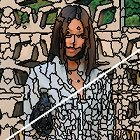
\includegraphics[height=1.65cm]{pictures/fash/w/cropped/w_010_contours}
	\end{subfigure}
	% EAMS %%%%%%%%%%%%%%%%%%%%%%%%%%%%%%%%%%%%%%%%%%%%%%%%%%%%%%%%%%%%%%%%%%%%%
	\begin{subfigure}[b]{0.02\textwidth}
		\rotatebox{90}{\small\hphantom{ai}\EAMS}
	\end{subfigure}
	\begin{subfigure}[b]{0.16\textwidth}
        \begin{center}
            \BSDS
        \end{center}
        \vskip -6px
		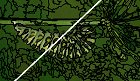
\includegraphics[height=1.65cm]{pictures/bsds500/eams/cropped/eams_35028_contours}
	\end{subfigure}
	\begin{subfigure}[b]{0.129\textwidth}
        \begin{center}
            \SBD
        \end{center}
        \vskip -6px
		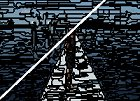
\includegraphics[height=1.65cm]{pictures/sbd/eams/cropped/eams_0004774_contours}
	\end{subfigure}
	\begin{subfigure}[b]{0.10\textwidth}
        \begin{center}
            \Fash
        \end{center}
        \vskip -6px
		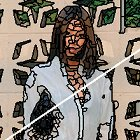
\includegraphics[height=1.65cm]{pictures/fash/eams/cropped/eams_010_contours}
	\end{subfigure}\\
	% NC %%%%%%%%%%%%%%%%%%%%%%%%%%%%%%%%%%%%%%%%%%%%%%%%%%%%%%%%%%%%%%%%%%%%%%%
	\begin{subfigure}[b]{0.02\textwidth}
		\rotatebox{90}{\small\hphantom{aaa}\NC}
	\end{subfigure}
	\begin{subfigure}[b]{0.16\textwidth}
		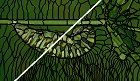
\includegraphics[height=1.65cm]{pictures/bsds500/nc/cropped/nc_35028_contours}
	\end{subfigure}
	\begin{subfigure}[b]{0.129\textwidth}
		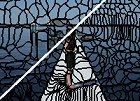
\includegraphics[height=1.65cm]{pictures/sbd/nc/cropped/nc_0004774_contours}
	\end{subfigure}
	\begin{subfigure}[b]{0.10\textwidth}
		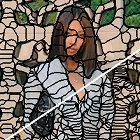
\includegraphics[height=1.65cm]{pictures/fash/nc/cropped/nc_010_contours}
	\end{subfigure}
	% FH %%%%%%%%%%%%%%%%%%%%%%%%%%%%%%%%%%%%%%%%%%%%%%%%%%%%%%%%%%%%%%%%%%%%%%%
	\begin{subfigure}[b]{0.02\textwidth}
		\rotatebox{90}{\small\hphantom{aaa}\FH}
	\end{subfigure}
	\begin{subfigure}[b]{0.16\textwidth}
		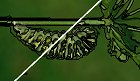
\includegraphics[height=1.65cm]{pictures/bsds500/fh/cropped/fh_35028_contours}
	\end{subfigure}
	\begin{subfigure}[b]{0.129\textwidth}
		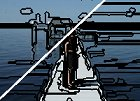
\includegraphics[height=1.65cm]{pictures/sbd/fh/cropped/fh_0004774_contours}
	\end{subfigure}
	\begin{subfigure}[b]{0.10\textwidth}
		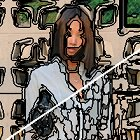
\includegraphics[height=1.65cm]{pictures/fash/fh/cropped/fh_010_contours}
	\end{subfigure}\\
	% RW %%%%%%%%%%%%%%%%%%%%%%%%%%%%%%%%%%%%%%%%%%%%%%%%%%%%%%%%%%%%%%%%%%%%%%%
	\begin{subfigure}[b]{0.02\textwidth}
		\rotatebox{90}{\small\hphantom{aaa}\RW}
	\end{subfigure}
	\begin{subfigure}[b]{0.16\textwidth}
		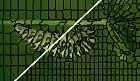
\includegraphics[height=1.65cm]{pictures/bsds500/rw/cropped/rw_35028_contours}
	\end{subfigure}
	\begin{subfigure}[b]{0.129\textwidth}
		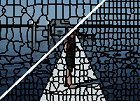
\includegraphics[height=1.65cm]{pictures/sbd/rw/cropped/rw_0004774_contours}
	\end{subfigure}
	\begin{subfigure}[b]{0.10\textwidth}
		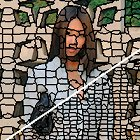
\includegraphics[height=1.65cm]{pictures/fash/rw/cropped/rw_010_contours}
	\end{subfigure}
	% QS %%%%%%%%%%%%%%%%%%%%%%%%%%%%%%%%%%%%%%%%%%%%%%%%%%%%%%%%%%%%%%%%%%%%%%%
	\begin{subfigure}[b]{0.02\textwidth}
		\rotatebox{90}{\small\hphantom{aaa}\QS}
	\end{subfigure}
	\begin{subfigure}[b]{0.16\textwidth}
		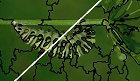
\includegraphics[height=1.65cm]{pictures/bsds500/qs/cropped/qs_35028_contours}
	\end{subfigure}
	\begin{subfigure}[b]{0.129\textwidth}
		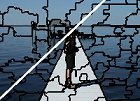
\includegraphics[height=1.65cm]{pictures/sbd/qs/cropped/qs_0004774_contours}
	\end{subfigure}
	\begin{subfigure}[b]{0.10\textwidth}
		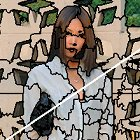
\includegraphics[height=1.65cm]{pictures/fash/qs/cropped/qs_010_contours}
	\end{subfigure}\\
	% PF %%%%%%%%%%%%%%%%%%%%%%%%%%%%%%%%%%%%%%%%%%%%%%%%%%%%%%%%%%%%%%%%%%%%%%%
	\begin{subfigure}[b]{0.02\textwidth}
		\rotatebox{90}{\small\hphantom{aaa}\PF}
	\end{subfigure}
	\begin{subfigure}[b]{0.16\textwidth}
		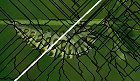
\includegraphics[height=1.65cm]{pictures/bsds500/pf/cropped/pf_35028_contours}
	\end{subfigure}
	\begin{subfigure}[b]{0.129\textwidth}
		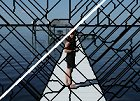
\includegraphics[height=1.65cm]{pictures/sbd/pf/cropped/pf_0004774_contours}
	\end{subfigure}
	\begin{subfigure}[b]{0.10\textwidth}
		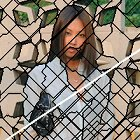
\includegraphics[height=1.65cm]{pictures/fash/pf/cropped/pf_010_contours}
	\end{subfigure}
	% TP %%%%%%%%%%%%%%%%%%%%%%%%%%%%%%%%%%%%%%%%%%%%%%%%%%%%%%%%%%%%%%%%%%%%%%%
	\begin{subfigure}[b]{0.02\textwidth}
		\rotatebox{90}{\small\hphantom{aaa}\TP}
	\end{subfigure}
	\begin{subfigure}[b]{0.16\textwidth}
		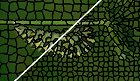
\includegraphics[height=1.65cm]{pictures/bsds500/tp/cropped/tp_35028_contours}
	\end{subfigure}
	\begin{subfigure}[b]{0.129\textwidth}
		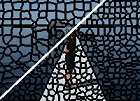
\includegraphics[height=1.65cm]{pictures/sbd/tp/cropped/tp_0004774_contours}
	\end{subfigure}
	\begin{subfigure}[b]{0.10\textwidth}
		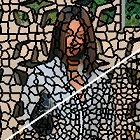
\includegraphics[height=1.65cm]{pictures/fash/tp/cropped/tp_010_contours}
	\end{subfigure}\\
	% CIS %%%%%%%%%%%%%%%%%%%%%%%%%%%%%%%%%%%%%%%%%%%%%%%%%%%%%%%%%%%%%%%%%%%%%%
	\begin{subfigure}[b]{0.02\textwidth}
		\rotatebox{90}{\small\hphantom{aai}\CIS}
	\end{subfigure}
	\begin{subfigure}[b]{0.16\textwidth}
		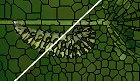
\includegraphics[height=1.65cm]{pictures/bsds500/cis/cropped/cis_35028_contours}
	\end{subfigure}
	\begin{subfigure}[b]{0.129\textwidth}
		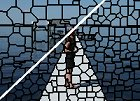
\includegraphics[height=1.65cm]{pictures/sbd/cis/cropped/cis_0004774_contours}
	\end{subfigure}
	\begin{subfigure}[b]{0.10\textwidth}
		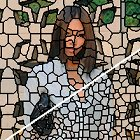
\includegraphics[height=1.65cm]{pictures/fash/cis/cropped/cis_010_contours}
	\end{subfigure}
	% SLIC %%%%%%%%%%%%%%%%%%%%%%%%%%%%%%%%%%%%%%%%%%%%%%%%%%%%%%%%%%%%%%%%%%%%%
	\begin{subfigure}[b]{0.02\textwidth}
		\rotatebox{90}{\small\hphantom{aa}\SLIC}
	\end{subfigure}
	\begin{subfigure}[b]{0.16\textwidth}
		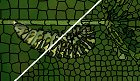
\includegraphics[height=1.65cm]{pictures/bsds500/slic/cropped/slic_35028_contours}
	\end{subfigure}
	\begin{subfigure}[b]{0.129\textwidth}
		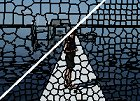
\includegraphics[height=1.65cm]{pictures/sbd/slic/cropped/slic_0004774_contours}
	\end{subfigure}
	\begin{subfigure}[b]{0.10\textwidth}
		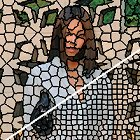
\includegraphics[height=1.65cm]{pictures/fash/slic/cropped/slic_010_contours}
	\end{subfigure}\\
	% CRS %%%%%%%%%%%%%%%%%%%%%%%%%%%%%%%%%%%%%%%%%%%%%%%%%%%%%%%%%%%%%%%%%%%%%%
	\begin{subfigure}[b]{0.02\textwidth}
		\rotatebox{90}{\small\hphantom{aai}\CRS}
	\end{subfigure}
	\begin{subfigure}[b]{0.16\textwidth}
		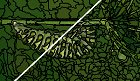
\includegraphics[height=1.65cm]{pictures/bsds500/crs/cropped/crs_35028_contours}
	\end{subfigure}
	\begin{subfigure}[b]{0.129\textwidth}
		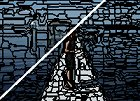
\includegraphics[height=1.65cm]{pictures/sbd/crs/cropped/crs_0004774_contours}
	\end{subfigure}
	\begin{subfigure}[b]{0.10\textwidth}
		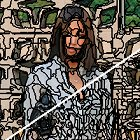
\includegraphics[height=1.65cm]{pictures/fash/crs/cropped/crs_010_contours}
	\end{subfigure}
	% ERS %%%%%%%%%%%%%%%%%%%%%%%%%%%%%%%%%%%%%%%%%%%%%%%%%%%%%%%%%%%%%%%%%%%%%%
	\begin{subfigure}[b]{0.02\textwidth}
		\rotatebox{90}{\small\hphantom{aai}\ERS}
	\end{subfigure}
	\begin{subfigure}[b]{0.16\textwidth}
		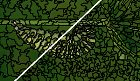
\includegraphics[height=1.65cm]{pictures/bsds500/ers/cropped/ers_35028_contours}
	\end{subfigure}
	\begin{subfigure}[b]{0.129\textwidth}
		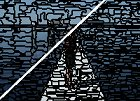
\includegraphics[height=1.65cm]{pictures/sbd/ers/cropped/ers_0004774_contours}
	\end{subfigure}
	\begin{subfigure}[b]{0.10\textwidth}
		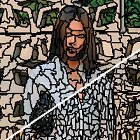
\includegraphics[height=1.65cm]{pictures/fash/ers/cropped/ers_010_contours}
	\end{subfigure}\\
	% PB %%%%%%%%%%%%%%%%%%%%%%%%%%%%%%%%%%%%%%%%%%%%%%%%%%%%%%%%%%%%%%%%%%%%%%
	\begin{subfigure}[b]{0.02\textwidth}
		\rotatebox{90}{\small\hphantom{aaa}\PB}
	\end{subfigure}
	\begin{subfigure}[b]{0.16\textwidth}
		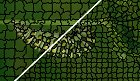
\includegraphics[height=1.65cm]{pictures/bsds500/pb/cropped/pb_35028_contours}
	\end{subfigure}
	\begin{subfigure}[b]{0.129\textwidth}
		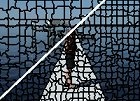
\includegraphics[height=1.65cm]{pictures/sbd/pb/cropped/pb_0004774_contours}
	\end{subfigure}
	\begin{subfigure}[b]{0.10\textwidth}
		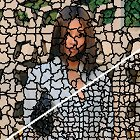
\includegraphics[height=1.65cm]{pictures/fash/pb/cropped/pb_010_contours}
	\end{subfigure}
	% SEEDS %%%%%%%%%%%%%%%%%%%%%%%%%%%%%%%%%%%%%%%%%%%%%%%%%%%%%%%%%%%%%%%%%%%%%%
	\begin{subfigure}[b]{0.02\textwidth}
		\rotatebox{90}{\small\hphantom{a}\SEEDS}
	\end{subfigure}
	\begin{subfigure}[b]{0.16\textwidth}
		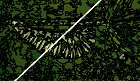
\includegraphics[height=1.65cm]{pictures/bsds500/seeds/cropped/seeds_35028_contours}
	\end{subfigure}
	\begin{subfigure}[b]{0.129\textwidth}
		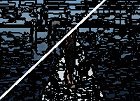
\includegraphics[height=1.65cm]{pictures/sbd/seeds/cropped/seeds_0004774_contours}
	\end{subfigure}
	\begin{subfigure}[b]{0.10\textwidth}
		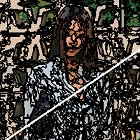
\includegraphics[height=1.65cm]{pictures/fash/seeds/cropped/seeds_010_contours}
	\end{subfigure}\\
	% TPS %%%%%%%%%%%%%%%%%%%%%%%%%%%%%%%%%%%%%%%%%%%%%%%%%%%%%%%%%%%%%%%%%%%%%%
	\begin{subfigure}[b]{0.02\textwidth}
		\rotatebox{90}{\small\hphantom{aai}\TPS}
	\end{subfigure}
	\begin{subfigure}[b]{0.16\textwidth}
		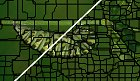
\includegraphics[height=1.65cm]{pictures/bsds500/tps/cropped/tps_35028_contours}
	\end{subfigure}
	\begin{subfigure}[b]{0.129\textwidth}
		\includegraphics[height=1.65cm]{pictures/sbd/tps/cropped/tps_0004774_contours}
	\end{subfigure}
	\begin{subfigure}[b]{0.10\textwidth}
		\includegraphics[height=1.65cm]{pictures/fash/tps/cropped/tps_010_contours}
	\end{subfigure}
	% VC %%%%%%%%%%%%%%%%%%%%%%%%%%%%%%%%%%%%%%%%%%%%%%%%%%%%%%%%%%%%%%%%%%%%%%
	\begin{subfigure}[b]{0.02\textwidth}
		\rotatebox{90}{\small\hphantom{aaa}\VC}
	\end{subfigure}
	\begin{subfigure}[b]{0.16\textwidth}
		\includegraphics[height=1.65cm]{pictures/bsds500/vc/cropped/vc_35028_contours}
	\end{subfigure}
	\begin{subfigure}[b]{0.129\textwidth}
		\includegraphics[height=1.65cm]{pictures/sbd/vc/cropped/vc_0004774_contours}
	\end{subfigure}
	\begin{subfigure}[b]{0.10\textwidth}
		\includegraphics[height=1.65cm]{pictures/fash/vc/cropped/vc_010_contours}
	\end{subfigure}\\
	% CCS %%%%%%%%%%%%%%%%%%%%%%%%%%%%%%%%%%%%%%%%%%%%%%%%%%%%%%%%%%%%%%%%%%%%%%
	\begin{subfigure}[b]{0.02\textwidth}
		\rotatebox{90}{\small\hphantom{aai}\CCS}
	\end{subfigure}
	\begin{subfigure}[b]{0.16\textwidth}
		\includegraphics[height=1.65cm]{pictures/bsds500/ccs/cropped/ccs_35028_contours}
	\end{subfigure}
	\begin{subfigure}[b]{0.129\textwidth}
		\includegraphics[height=1.65cm]{pictures/sbd/ccs/cropped/ccs_0004774_contours}
	\end{subfigure}
	\begin{subfigure}[b]{0.10\textwidth}
		\includegraphics[height=1.65cm]{pictures/fash/ccs/cropped/ccs_010_contours}
	\end{subfigure}
	% CW %%%%%%%%%%%%%%%%%%%%%%%%%%%%%%%%%%%%%%%%%%%%%%%%%%%%%%%%%%%%%%%%%%%%%%
	\begin{subfigure}[b]{0.02\textwidth}
		\rotatebox{90}{\small\hphantom{aaa}\CW}
	\end{subfigure}
	\begin{subfigure}[b]{0.16\textwidth}
		\includegraphics[height=1.65cm]{pictures/bsds500/cw/cropped/cw_35028_contours}
	\end{subfigure}
	\begin{subfigure}[b]{0.129\textwidth}
		\includegraphics[height=1.65cm]{pictures/sbd/cw/cropped/cw_0004774_contours}
	\end{subfigure}
	\begin{subfigure}[b]{0.10\textwidth}
		\includegraphics[height=1.65cm]{pictures/fash/cw/cropped/cw_010_contours}
	\end{subfigure}\\
	% ERGC %%%%%%%%%%%%%%%%%%%%%%%%%%%%%%%%%%%%%%%%%%%%%%%%%%%%%%%%%%%%%%%%%%%%%%
	\begin{subfigure}[b]{0.02\textwidth}
		\rotatebox{90}{\small\hphantom{aa}\ERGC}
	\end{subfigure}
	\begin{subfigure}[b]{0.16\textwidth}
		\includegraphics[height=1.65cm]{pictures/bsds500/ergc/cropped/ergc_35028_contours}
	\end{subfigure}
	\begin{subfigure}[b]{0.129\textwidth}
		\includegraphics[height=1.65cm]{pictures/sbd/ergc/cropped/ergc_0004774_contours}
	\end{subfigure}
	\begin{subfigure}[b]{0.10\textwidth}
		\includegraphics[height=1.65cm]{pictures/fash/ergc/cropped/ergc_010_contours}
	\end{subfigure}
	% MSS %%%%%%%%%%%%%%%%%%%%%%%%%%%%%%%%%%%%%%%%%%%%%%%%%%%%%%%%%%%%%%%%%%%%%%
	\begin{subfigure}[b]{0.02\textwidth}
		\rotatebox{90}{\small\hphantom{aai}\MSS}
	\end{subfigure}
	\begin{subfigure}[b]{0.16\textwidth}
		\includegraphics[height=1.65cm]{pictures/bsds500/mss/cropped/mss_35028_contours}
	\end{subfigure}
	\begin{subfigure}[b]{0.129\textwidth}
		\includegraphics[height=1.65cm]{pictures/sbd/mss/cropped/mss_0004774_contours}
	\end{subfigure}
	\begin{subfigure}[b]{0.10\textwidth}
		\includegraphics[height=1.65cm]{pictures/fash/mss/cropped/mss_010_contours}
	\end{subfigure}\\
	% preSLIC %%%%%%%%%%%%%%%%%%%%%%%%%%%%%%%%%%%%%%%%%%%%%%%%%%%%%%%%%%%%%%%%%%%%%%
	\begin{subfigure}[b]{0.02\textwidth}
		\rotatebox{90}{\small\hphantom{a}\preSLIC}
	\end{subfigure}
	\begin{subfigure}[b]{0.16\textwidth}
		\includegraphics[height=1.65cm]{pictures/bsds500/preslic/cropped/preslic_35028_contours}
	\end{subfigure}
	\begin{subfigure}[b]{0.129\textwidth}
		\includegraphics[height=1.65cm]{pictures/sbd/preslic/cropped/preslic_0004774_contours}
	\end{subfigure}
	\begin{subfigure}[b]{0.10\textwidth}
		\includegraphics[height=1.65cm]{pictures/fash/preslic/cropped/preslic_010_contours}
	\end{subfigure}
	% WP %%%%%%%%%%%%%%%%%%%%%%%%%%%%%%%%%%%%%%%%%%%%%%%%%%%%%%%%%%%%%%%%%%%%%%
	\begin{subfigure}[b]{0.02\textwidth}
		\rotatebox{90}{\small\hphantom{aaa}\WP}
	\end{subfigure}
	\begin{subfigure}[b]{0.16\textwidth}
		\includegraphics[height=1.65cm]{pictures/bsds500/wp/cropped/wp_35028_contours}
	\end{subfigure}
	\begin{subfigure}[b]{0.129\textwidth}
		\includegraphics[height=1.65cm]{pictures/sbd/wp/cropped/wp_0004774_contours}
	\end{subfigure}
	\begin{subfigure}[b]{0.10\textwidth}
		\includegraphics[height=1.65cm]{pictures/fash/wp/cropped/wp_010_contours}
	\end{subfigure}\\
	% ETPS %%%%%%%%%%%%%%%%%%%%%%%%%%%%%%%%%%%%%%%%%%%%%%%%%%%%%%%%%%%%%%%%%%%%%%
	\begin{subfigure}[b]{0.02\textwidth}
		\rotatebox{90}{\small\hphantom{aa}\ETPS}
	\end{subfigure}
	\begin{subfigure}[b]{0.16\textwidth}
		\includegraphics[height=1.65cm]{pictures/bsds500/etps/cropped/etps_35028_contours}
	\end{subfigure}
	\begin{subfigure}[b]{0.129\textwidth}
		\includegraphics[height=1.65cm]{pictures/sbd/etps/cropped/etps_0004774_contours}
	\end{subfigure}
	\begin{subfigure}[b]{0.10\textwidth}
		\includegraphics[height=1.65cm]{pictures/fash/etps/cropped/etps_010_contours}
	\end{subfigure}
	% LSC %%%%%%%%%%%%%%%%%%%%%%%%%%%%%%%%%%%%%%%%%%%%%%%%%%%%%%%%%%%%%%%%%%%%%%
	\begin{subfigure}[b]{0.02\textwidth}
		\rotatebox{90}{\small\hphantom{aai}\LSC}
	\end{subfigure}
	\begin{subfigure}[b]{0.16\textwidth}
		\includegraphics[height=1.65cm]{pictures/bsds500/lsc/cropped/lsc_35028_contours}
	\end{subfigure}
	\begin{subfigure}[b]{0.129\textwidth}
		\includegraphics[height=1.65cm]{pictures/sbd/lsc/cropped/lsc_0004774_contours}
	\end{subfigure}
	\begin{subfigure}[b]{0.10\textwidth}
		\includegraphics[height=1.65cm]{pictures/fash/lsc/cropped/lsc_010_contours}
	\end{subfigure}\\
	% POISE %%%%%%%%%%%%%%%%%%%%%%%%%%%%%%%%%%%%%%%%%%%%%%%%%%%%%%%%%%%%%%%%%%%%%%
	\begin{subfigure}[b]{0.02\textwidth}
		\rotatebox{90}{\small\hphantom{a}\POISE}
	\end{subfigure}
	\begin{subfigure}[b]{0.16\textwidth}
		\includegraphics[height=1.65cm]{pictures/bsds500/poise/cropped/poise_35028_contours}
	\end{subfigure}
	\begin{subfigure}[b]{0.129\textwidth}
		\includegraphics[height=1.65cm]{pictures/sbd/poise/cropped/poise_0004774_contours}
	\end{subfigure}
	\begin{subfigure}[b]{0.10\textwidth}
		\includegraphics[height=1.65cm]{pictures/fash/poise/cropped/poise_010_contours}
	\end{subfigure}
	% SEAW %%%%%%%%%%%%%%%%%%%%%%%%%%%%%%%%%%%%%%%%%%%%%%%%%%%%%%%%%%%%%%%%%%%%%%
	\begin{subfigure}[b]{0.02\textwidth}
		\rotatebox{90}{\small\hphantom{ai}\SEAW}
	\end{subfigure}
	\begin{subfigure}[b]{0.16\textwidth}
		\includegraphics[height=1.65cm]{pictures/bsds500/seaw/cropped/seaw_35028_contours}
	\end{subfigure}
	\begin{subfigure}[b]{0.129\textwidth}
		\includegraphics[height=1.65cm]{pictures/sbd/seaw/cropped/seaw_0004774_contours}
	\end{subfigure}
	\begin{subfigure}[b]{0.10\textwidth}
		\includegraphics[height=1.65cm]{pictures/fash/seaw/cropped/seaw_010_contours}
	\end{subfigure}
	\caption{Qualitative results on the \BSDS, \SBD and \Fash datasets. Excerpts from the
	images in Figure \ref{fig:datasets} are shown for $K \approx 400$ in the upper left corner
	and $K \approx 1200$ in the lower right corner. Superpixel boundaries are depicted
	in black; best viewed in color. We judge visual quality on the basis of
	boundary adherence, compactness, smoothness and regularity.
	Boundary adherence can be judged both on the caterpillar image as well 
	as on the woman image -- the caterpillar's boundaries are hard to detect and 
	the woman's face exhibits small details. In contrast, compactness, regularity and smoothness 
	can be evaluated considering the background in the caterpillar and see images.
	\textbf{Best viewed in color.}}
	\label{fig:experiments-qualitative-bsds500-sbd-fash}
\end{figure*}

\def\NYUCroppedScale{0.18}
\def\SUNRGBDCroppedScale{0.14}
\begin{figure*}
	\centering
	% NC %%%%%%%%%%%%%%%%%%%%%%%%%%%%%%%%%%%%%%%%%%%%%%%%%%%%%%%%%%%%%%%%%%%%%%%%
	\begin{subfigure}[b]{0.02\textwidth}
		\rotatebox{90}{\small\hphantom{aaa}\NC}
	\end{subfigure}
	\begin{subfigure}[b]{0.1375\textwidth}
		\begin{center}
			\NYU
		\end{center}
		\vskip -6px
		\includegraphics[height=1.65cm]{pictures/nyuv2/nc/cropped/nc_00000561_contours}
	\end{subfigure}
	\begin{subfigure}[b]{0.129\textwidth}
		\begin{center}
			\NYU
		\end{center}
		\vskip -6px
		\includegraphics[height=1.65cm]{pictures/nyuv2/nc/cropped/nc_00000285_contours_scaled}
	\end{subfigure}
	% RW %%%%%%%%%%%%%%%%%%%%%%%%%%%%%%%%%%%%%%%%%%%%%%%%%%%%%%%%%%%%%%%%%%%%%%%%
	\begin{subfigure}[b]{0.02\textwidth}
		\rotatebox{90}{\small\hphantom{aaa}\RW}
	\end{subfigure}
	\begin{subfigure}[b]{0.1375\textwidth}
		\begin{center}
			\NYU
		\end{center}
		\vskip -6px
		\includegraphics[height=1.65cm]{pictures/nyuv2/rw/cropped/rw_00000561_contours}
	\end{subfigure}
	\begin{subfigure}[b]{0.129\textwidth}
		\begin{center}
			\NYU
		\end{center}
		\vskip -6px
		\includegraphics[height=1.65cm]{pictures/nyuv2/rw/cropped/rw_00000285_contours_scaled}
	\end{subfigure}
	% SEAW %%%%%%%%%%%%%%%%%%%%%%%%%%%%%%%%%%%%%%%%%%%%%%%%%%%%%%%%%%%%%%%%%%%%%%%%
	\begin{subfigure}[b]{0.02\textwidth}
		\rotatebox{90}{\small\hphantom{ai}\SEAW}
	\end{subfigure}
	\begin{subfigure}[b]{0.1375\textwidth}
		\begin{center}
			\NYU
		\end{center}
		\vskip -6px
		\includegraphics[height=1.65cm]{pictures/nyuv2/seaw/cropped/seaw_00000561_contours}
	\end{subfigure}
	\begin{subfigure}[b]{0.129\textwidth}
		\begin{center}
			\NYU
		\end{center}
		\vskip -6px
		\includegraphics[height=1.65cm]{pictures/nyuv2/seaw/cropped/seaw_00000285_contours_scaled}
	\end{subfigure}\\[4px]
	% W %%%%%%%%%%%%%%%%%%%%%%%%%%%%%%%%%%%%%%%%%%%%%%%%%%%%%%%%%%%%%%%%%%%%%%%%
	\begin{subfigure}[b]{0.02\textwidth}
		\rotatebox{90}{\small\hphantom{aaai}\W}
	\end{subfigure}
	\begin{subfigure}[b]{0.1375\textwidth}
		\begin{center}
			\NYU
		\end{center}
		\vskip -6px
		\includegraphics[height=1.65cm]{pictures/nyuv2/w/cropped/w_00000561_contours}
	\end{subfigure}
	\begin{subfigure}[b]{0.129\textwidth}
		\begin{center}
			\SUNRGBD
		\end{center}
		\vskip -6px
		\includegraphics[height=1.65cm]{pictures/sunrgbd/w/cropped/w_00004732_contours}
	\end{subfigure}
	% EAMS %%%%%%%%%%%%%%%%%%%%%%%%%%%%%%%%%%%%%%%%%%%%%%%%%%%%%%%%%%%%%%%%%%%%%%%%
	\begin{subfigure}[b]{0.02\textwidth}
		\rotatebox{90}{\small\hphantom{ai}\EAMS}
	\end{subfigure}
	\begin{subfigure}[b]{0.1375\textwidth}
		\begin{center}
			\NYU
		\end{center}
		\vskip -6px
		\includegraphics[height=1.65cm]{pictures/nyuv2/eams/cropped/eams_00000561_contours}
	\end{subfigure}
	\begin{subfigure}[b]{0.129\textwidth}
		\begin{center}
			\SUNRGBD
		\end{center}
		\vskip -6px
		\includegraphics[height=1.65cm]{pictures/sunrgbd/eams/cropped/eams_00004732_contours}
	\end{subfigure}
	% FH %%%%%%%%%%%%%%%%%%%%%%%%%%%%%%%%%%%%%%%%%%%%%%%%%%%%%%%%%%%%%%%%%%%%%%%%
	\begin{subfigure}[b]{0.02\textwidth}
		\rotatebox{90}{\small\hphantom{aaa}\FH}
	\end{subfigure}
	\begin{subfigure}[b]{0.1375\textwidth}
		\begin{center}
			\NYU
		\end{center}
		\vskip -6px
		\includegraphics[height=1.65cm]{pictures/nyuv2/fh/cropped/fh_00000561_contours}
	\end{subfigure}
	\begin{subfigure}[b]{0.129\textwidth}
		\begin{center}
			\SUNRGBD
		\end{center}
		\vskip -6px
		\includegraphics[height=1.65cm]{pictures/sunrgbd/fh/cropped/fh_00004732_contours}
	\end{subfigure}\\
	% QS %%%%%%%%%%%%%%%%%%%%%%%%%%%%%%%%%%%%%%%%%%%%%%%%%%%%%%%%%%%%%%%%%%%%%%%%
	\begin{subfigure}[b]{0.02\textwidth}
		\rotatebox{90}{\small\hphantom{aaa}\QS}
	\end{subfigure}
	\begin{subfigure}[b]{0.1375\textwidth}
		\includegraphics[height=1.65cm]{pictures/nyuv2/qs/cropped/qs_00000561_contours}
	\end{subfigure}
	\begin{subfigure}[b]{0.129\textwidth}
		\includegraphics[height=1.65cm]{pictures/sunrgbd/qs/cropped/qs_00004732_contours}
	\end{subfigure}
	% PF %%%%%%%%%%%%%%%%%%%%%%%%%%%%%%%%%%%%%%%%%%%%%%%%%%%%%%%%%%%%%%%%%%%%%%%%
	\begin{subfigure}[b]{0.02\textwidth}
		\rotatebox{90}{\small\hphantom{aaa}\PF}
	\end{subfigure}
	\begin{subfigure}[b]{0.1375\textwidth}
		\includegraphics[height=1.65cm]{pictures/nyuv2/pf/cropped/pf_00000561_contours}
	\end{subfigure}
	\begin{subfigure}[b]{0.129\textwidth}
		\includegraphics[height=1.65cm]{pictures/sunrgbd/pf/cropped/pf_00004732_contours}
	\end{subfigure}
	% TP %%%%%%%%%%%%%%%%%%%%%%%%%%%%%%%%%%%%%%%%%%%%%%%%%%%%%%%%%%%%%%%%%%%%%%%%
	\begin{subfigure}[b]{0.02\textwidth}
		\rotatebox{90}{\small\hphantom{aaa}\TP}
	\end{subfigure}
	\begin{subfigure}[b]{0.1375\textwidth}
		\includegraphics[height=1.65cm]{pictures/nyuv2/tp/cropped/tp_00000561_contours}
	\end{subfigure}
	\begin{subfigure}[b]{0.129\textwidth}
		\includegraphics[height=1.65cm]{pictures/sunrgbd/tp/cropped/tp_00004732_contours}
	\end{subfigure}\\
	% CIS %%%%%%%%%%%%%%%%%%%%%%%%%%%%%%%%%%%%%%%%%%%%%%%%%%%%%%%%%%%%%%%%%%%%%%%%
	\begin{subfigure}[b]{0.02\textwidth}
		\rotatebox{90}{\small\hphantom{aai}\CIS}
	\end{subfigure}
	\begin{subfigure}[b]{0.1375\textwidth}
		\includegraphics[height=1.65cm]{pictures/nyuv2/cis/cropped/cis_00000561_contours}
	\end{subfigure}
	\begin{subfigure}[b]{0.129\textwidth}
		\includegraphics[height=1.65cm]{pictures/sunrgbd/cis/cropped/cis_00004732_contours}
	\end{subfigure}
	% SLIC %%%%%%%%%%%%%%%%%%%%%%%%%%%%%%%%%%%%%%%%%%%%%%%%%%%%%%%%%%%%%%%%%%%%%%%%
	\begin{subfigure}[b]{0.02\textwidth}
		\rotatebox{90}{\small\hphantom{aa}\SLIC}
	\end{subfigure}
	\begin{subfigure}[b]{0.1375\textwidth}
		\includegraphics[height=1.65cm]{pictures/nyuv2/slic/cropped/slic_00000561_contours}
	\end{subfigure}
	\begin{subfigure}[b]{0.129\textwidth}
		\includegraphics[height=1.65cm]{pictures/sunrgbd/slic/cropped/slic_00004732_contours}
	\end{subfigure}
	% CRS %%%%%%%%%%%%%%%%%%%%%%%%%%%%%%%%%%%%%%%%%%%%%%%%%%%%%%%%%%%%%%%%%%%%%%%%
	\begin{subfigure}[b]{0.02\textwidth}
		\rotatebox{90}{\small\hphantom{aai}\CRS}
	\end{subfigure}
	\begin{subfigure}[b]{0.1375\textwidth}
		\includegraphics[height=1.65cm]{pictures/nyuv2/crs/cropped/crs_00000561_contours}
	\end{subfigure}
	\begin{subfigure}[b]{0.129\textwidth}
		\includegraphics[height=1.65cm]{pictures/sunrgbd/crs/cropped/crs_00004732_contours}
	\end{subfigure}\\
	% ERS %%%%%%%%%%%%%%%%%%%%%%%%%%%%%%%%%%%%%%%%%%%%%%%%%%%%%%%%%%%%%%%%%%%%%%%%
	\begin{subfigure}[b]{0.02\textwidth}
		\rotatebox{90}{\small\hphantom{aai}\ERS}
	\end{subfigure}
	\begin{subfigure}[b]{0.1375\textwidth}
		\includegraphics[height=1.65cm]{pictures/nyuv2/ers/cropped/ers_00000561_contours}
	\end{subfigure}
	\begin{subfigure}[b]{0.129\textwidth}
		\includegraphics[height=1.65cm]{pictures/sunrgbd/ers/cropped/ers_00004732_contours}
	\end{subfigure}
	% PB %%%%%%%%%%%%%%%%%%%%%%%%%%%%%%%%%%%%%%%%%%%%%%%%%%%%%%%%%%%%%%%%%%%%%%%%
	\begin{subfigure}[b]{0.02\textwidth}
		\rotatebox{90}{\small\hphantom{aaa}\PB}
	\end{subfigure}
	\begin{subfigure}[b]{0.1375\textwidth}
		\includegraphics[height=1.65cm]{pictures/nyuv2/pb/cropped/pb_00000561_contours}
	\end{subfigure}
	\begin{subfigure}[b]{0.129\textwidth}
		\includegraphics[height=1.65cm]{pictures/sunrgbd/pb/cropped/pb_00004732_contours}
	\end{subfigure}
	% DASP %%%%%%%%%%%%%%%%%%%%%%%%%%%%%%%%%%%%%%%%%%%%%%%%%%%%%%%%%%%%%%%%%%%%%%%%
	\begin{subfigure}[b]{0.02\textwidth}
		\rotatebox{90}{\small\hphantom{aa}\DASP}
	\end{subfigure}
	\begin{subfigure}[b]{0.1375\textwidth}
		\includegraphics[height=1.65cm]{pictures/nyuv2/dasp/cropped/dasp_00000561_contours}
	\end{subfigure}
	\begin{subfigure}[b]{0.129\textwidth}
		\includegraphics[height=1.65cm]{pictures/sunrgbd/dasp/cropped/dasp_00004732_contours}
	\end{subfigure}\\
	% SEEDS %%%%%%%%%%%%%%%%%%%%%%%%%%%%%%%%%%%%%%%%%%%%%%%%%%%%%%%%%%%%%%%%%%%%%%%%
	\begin{subfigure}[b]{0.02\textwidth}
		\rotatebox{90}{\small\hphantom{a}\SEEDS}
	\end{subfigure}
	\begin{subfigure}[b]{0.1375\textwidth}
		\includegraphics[height=1.65cm]{pictures/nyuv2/seeds/cropped/seeds_00000561_contours}
	\end{subfigure}
	\begin{subfigure}[b]{0.129\textwidth}
		\includegraphics[height=1.65cm]{pictures/sunrgbd/seeds/cropped/seeds_00004732_contours}
	\end{subfigure}
	% TPS %%%%%%%%%%%%%%%%%%%%%%%%%%%%%%%%%%%%%%%%%%%%%%%%%%%%%%%%%%%%%%%%%%%%%%%%
	\begin{subfigure}[b]{0.02\textwidth}
		\rotatebox{90}{\small\hphantom{aai}\TPS}
	\end{subfigure}
	\begin{subfigure}[b]{0.1375\textwidth}
		\includegraphics[height=1.65cm]{pictures/nyuv2/tps/cropped/tps_00000561_contours}
	\end{subfigure}
	\begin{subfigure}[b]{0.129\textwidth}
		\includegraphics[height=1.65cm]{pictures/sunrgbd/tps/cropped/tps_00004732_contours}
	\end{subfigure}
	% VC %%%%%%%%%%%%%%%%%%%%%%%%%%%%%%%%%%%%%%%%%%%%%%%%%%%%%%%%%%%%%%%%%%%%%%%%
	\begin{subfigure}[b]{0.02\textwidth}
		\rotatebox{90}{\small\hphantom{aaai}\VC}
	\end{subfigure}
	\begin{subfigure}[b]{0.1375\textwidth}
		\includegraphics[height=1.65cm]{pictures/nyuv2/vc/cropped/vc_00000561_contours}
	\end{subfigure}
	\begin{subfigure}[b]{0.129\textwidth}
		\includegraphics[height=1.65cm]{pictures/sunrgbd/vc/cropped/vc_00004732_contours}
	\end{subfigure}\\
	% CCS %%%%%%%%%%%%%%%%%%%%%%%%%%%%%%%%%%%%%%%%%%%%%%%%%%%%%%%%%%%%%%%%%%%%%%%%
	\begin{subfigure}[b]{0.02\textwidth}
		\rotatebox{90}{\small\hphantom{aai}\CCS}
	\end{subfigure}
	\begin{subfigure}[b]{0.1375\textwidth}
		\includegraphics[height=1.65cm]{pictures/nyuv2/ccs/cropped/ccs_00000561_contours}
	\end{subfigure}
	\begin{subfigure}[b]{0.129\textwidth}
		\includegraphics[height=1.65cm]{pictures/sunrgbd/ccs/cropped/ccs_00004732_contours}
	\end{subfigure}
	% VCCS %%%%%%%%%%%%%%%%%%%%%%%%%%%%%%%%%%%%%%%%%%%%%%%%%%%%%%%%%%%%%%%%%%%%%%%%
	\begin{subfigure}[b]{0.02\textwidth}
		\rotatebox{90}{\small\hphantom{aa}\VCCS}
	\end{subfigure}
	\begin{subfigure}[b]{0.1375\textwidth}
		\includegraphics[height=1.65cm]{pictures/nyuv2/vccs/cropped/vccs_00000561_contours}
	\end{subfigure}
	\begin{subfigure}[b]{0.129\textwidth}
		\includegraphics[height=1.65cm]{pictures/sunrgbd/vccs/cropped/vccs_00004732_contours}
	\end{subfigure}
	% CW %%%%%%%%%%%%%%%%%%%%%%%%%%%%%%%%%%%%%%%%%%%%%%%%%%%%%%%%%%%%%%%%%%%%%%%%
	\begin{subfigure}[b]{0.02\textwidth}
		\rotatebox{90}{\small\hphantom{aaa}\CW}
	\end{subfigure}
	\begin{subfigure}[b]{0.1375\textwidth}
		\includegraphics[height=1.65cm]{pictures/nyuv2/cw/cropped/cw_00000561_contours}
	\end{subfigure}
	\begin{subfigure}[b]{0.129\textwidth}
		\includegraphics[height=1.65cm]{pictures/sunrgbd/cw/cropped/cw_00004732_contours}
	\end{subfigure}\\
	% ERGC %%%%%%%%%%%%%%%%%%%%%%%%%%%%%%%%%%%%%%%%%%%%%%%%%%%%%%%%%%%%%%%%%%%%%%%%
	\begin{subfigure}[b]{0.02\textwidth}
		\rotatebox{90}{\small\hphantom{aa}\ERGC}
	\end{subfigure}
	\begin{subfigure}[b]{0.1375\textwidth}
		\includegraphics[height=1.65cm]{pictures/nyuv2/ergc/cropped/ergc_00000561_contours}
	\end{subfigure}
	\begin{subfigure}[b]{0.129\textwidth}
		\includegraphics[height=1.65cm]{pictures/sunrgbd/ergc/cropped/ergc_00004732_contours}
	\end{subfigure}
	% MSS %%%%%%%%%%%%%%%%%%%%%%%%%%%%%%%%%%%%%%%%%%%%%%%%%%%%%%%%%%%%%%%%%%%%%%%%
	\begin{subfigure}[b]{0.02\textwidth}
		\rotatebox{90}{\small\hphantom{aai}\MSS}
	\end{subfigure}
	\begin{subfigure}[b]{0.1375\textwidth}
		\includegraphics[height=1.65cm]{pictures/nyuv2/mss/cropped/mss_00000561_contours}
	\end{subfigure}
	\begin{subfigure}[b]{0.129\textwidth}
		\includegraphics[height=1.65cm]{pictures/sunrgbd/mss/cropped/mss_00004732_contours}
	\end{subfigure}
	% preSLIC %%%%%%%%%%%%%%%%%%%%%%%%%%%%%%%%%%%%%%%%%%%%%%%%%%%%%%%%%%%%%%%%%%%%%%%%
	\begin{subfigure}[b]{0.02\textwidth}
		\rotatebox{90}{\small\hphantom{a}\preSLIC}
	\end{subfigure}
	\begin{subfigure}[b]{0.1375\textwidth}
		\includegraphics[height=1.65cm]{pictures/nyuv2/preslic/cropped/preslic_00000561_contours}
	\end{subfigure}
	\begin{subfigure}[b]{0.129\textwidth}
		\includegraphics[height=1.65cm]{pictures/sunrgbd/preslic/cropped/preslic_00004732_contours}
	\end{subfigure}\\
	% WP %%%%%%%%%%%%%%%%%%%%%%%%%%%%%%%%%%%%%%%%%%%%%%%%%%%%%%%%%%%%%%%%%%%%%%%%
	\begin{subfigure}[b]{0.02\textwidth}
		\rotatebox{90}{\small\hphantom{aaa}\WP}
	\end{subfigure}
	\begin{subfigure}[b]{0.1375\textwidth}
		\includegraphics[height=1.65cm]{pictures/nyuv2/wp/cropped/wp_00000561_contours}
	\end{subfigure}
	\begin{subfigure}[b]{0.129\textwidth}
		\includegraphics[height=1.65cm]{pictures/sunrgbd/wp/cropped/wp_00004732_contours}
	\end{subfigure}
	% LRW %%%%%%%%%%%%%%%%%%%%%%%%%%%%%%%%%%%%%%%%%%%%%%%%%%%%%%%%%%%%%%%%%%%%%%%%
	%\begin{subfigure}[b]{0.02\textwidth}
	%	\rotatebox{90}{\small\LRW}
	%\end{subfigure}
	%\begin{subfigure}[b]{0.1375\textwidth}
	%	\includegraphics[height=1.65cm]{pictures/nyuv2/lrw/cropped/lrw_00000561_contours}
	%\end{subfigure}
	%\begin{subfigure}[b]{0.129\textwidth}
	%	\includegraphics[height=1.65cm]{pictures/nyuv2/lrw/cropped/lrw_00000561_contours}
	%\end{subfigure}\\
	% ETPS %%%%%%%%%%%%%%%%%%%%%%%%%%%%%%%%%%%%%%%%%%%%%%%%%%%%%%%%%%%%%%%%%%%%%%%%
	\begin{subfigure}[b]{0.02\textwidth}
		\rotatebox{90}{\small\hphantom{aa}\ETPS}
	\end{subfigure}
	\begin{subfigure}[b]{0.1375\textwidth}
		\includegraphics[height=1.65cm]{pictures/nyuv2/etps/cropped/etps_00000561_contours}
	\end{subfigure}
	\begin{subfigure}[b]{0.129\textwidth}
		\includegraphics[height=1.65cm]{pictures/sunrgbd/etps/cropped/etps_00004732_contours}
	\end{subfigure}
	% LSC %%%%%%%%%%%%%%%%%%%%%%%%%%%%%%%%%%%%%%%%%%%%%%%%%%%%%%%%%%%%%%%%%%%%%%%%
	\begin{subfigure}[b]{0.02\textwidth}
		\rotatebox{90}{\small\hphantom{aaa}\LSC}
	\end{subfigure}
	\begin{subfigure}[b]{0.1375\textwidth}
		\includegraphics[height=1.65cm]{pictures/nyuv2/lsc/cropped/lsc_00000561_contours}
	\end{subfigure}
	\begin{subfigure}[b]{0.129\textwidth}
		\includegraphics[height=1.65cm]{pictures/sunrgbd/lsc/cropped/lsc_00004732_contours}
	\end{subfigure}\\
	% POISE %%%%%%%%%%%%%%%%%%%%%%%%%%%%%%%%%%%%%%%%%%%%%%%%%%%%%%%%%%%%%%%%%%%%%%%%
	\begin{subfigure}[b]{0.02\textwidth}
		\rotatebox{90}{\small\hphantom{a}\POISE}
	\end{subfigure}
	\begin{subfigure}[b]{0.1375\textwidth}
		\includegraphics[height=1.65cm]{pictures/nyuv2/poise/cropped/poise_00000561_contours}
	\end{subfigure}
	\begin{subfigure}[b]{0.129\textwidth}
		\includegraphics[height=1.65cm]{pictures/sunrgbd/poise/cropped/poise_00004732_contours}
	\end{subfigure}
	% Puffer
	\begin{subfigure}[b]{0.02\textwidth}
		\hphantom{aa}
	\end{subfigure}
	\begin{subfigure}[b]{0.1375\textwidth}
		\hphantom{aaaaaaaaaaaaaaaaaaaaaaaaaaaaaii}
	\end{subfigure}
	\begin{subfigure}[b]{0.129\textwidth}
		\hphantom{aaaaaaaaaaaaaaaaaaaaaaaaaaa}
	\end{subfigure}
	% Puffer
	\begin{subfigure}[b]{0.02\textwidth}
		\hphantom{aa}
	\end{subfigure}
	\begin{subfigure}[b]{0.1375\textwidth}
		\hphantom{aaaaaaaaaaaaaaaaaaaaaaaaaaaaii}
	\end{subfigure}
	\begin{subfigure}[b]{0.129\textwidth}
		\hphantom{aaaaaaaaaaaaaaaaaaaaaaaaaaa}
	\end{subfigure}
	\caption{Qualitative results on the \NYU and \SUNRGBD datasets. Excerpts from the images
	in Figure \ref{fig:datasets} are shown for $K \approx 400$ in the upper left corner
	and $K \approx 1200$ in the lower right corner. Superpixel boundaries are depicted in black; best viewed in color.
	\NC, \RW and \SEAW could not be evaluated on the \SUNRGBD dataset due
	to exhaustive memory usage of the corresponding MatLab implementations.
	Therefore, results for the \NYU dataset are shown.
    Visual quality is judged regarding boundary adherence, compactness,
	smoothness and regularity. We also find
	that depth information, as used in \DASP and \VCCS, may help resemble the underlying 3D-structure.
	\textbf{Best viewed in color.}}
	\label{fig:experiments-qualitative-nyuv2-sunrgbd}
\end{figure*}
\begin{figure*}
	\centering
	% SLIC %%%%%%%%%%%%%%%%%%%%%%%%%%%%%%%%%%%%%%%%%%%%%%%%%%%%%%%%%%%%%%%%%%%%%%%%
	\begin{subfigure}[b]{0.02\textwidth}
		\rotatebox{90}{\small\hphantom{aa}\SLIC}
	\end{subfigure}
	\begin{subfigure}[b]{0.141\textwidth}
		\includegraphics[height=1.525cm]{pictures/compactness/bsds500/slic/score/1/cropped/slic_35028_contours}
	\end{subfigure}
	\begin{subfigure}[b]{0.141\textwidth}
		\includegraphics[height=1.525cm]{pictures/compactness/bsds500/slic/score/10/cropped/slic_35028_contours}
	\end{subfigure}
	\begin{subfigure}[b]{0.141\textwidth}
		\includegraphics[height=1.525cm]{pictures/compactness/bsds500/slic/score/80/cropped/slic_35028_contours}
	\end{subfigure}
	% CRS %%%%%%%%%%%%%%%%%%%%%%%%%%%%%%%%%%%%%%%%%%%%%%%%%%%%%%%%%%%%%%%%%%%%%%%%
	\begin{subfigure}[b]{0.02\textwidth}
		\rotatebox{90}{\small\hphantom{aai}\CRS}
	\end{subfigure}
	\begin{subfigure}[b]{0.141\textwidth}
		\includegraphics[height=1.525cm]{pictures/compactness/bsds500/crs/score/0.001/cropped/crs_35028_contours}
	\end{subfigure}
	\begin{subfigure}[b]{0.141\textwidth}
		\includegraphics[height=1.525cm]{pictures/compactness/bsds500/crs/score/0.01/cropped/crs_35028_contours}
	\end{subfigure}
	\begin{subfigure}[b]{0.141\textwidth}
		\includegraphics[height=1.525cm]{pictures/compactness/bsds500/crs/score/0.1/cropped/crs_35028_contours}
	\end{subfigure}
	\caption{The influence of a low, on the left, and high, on the right, compactness parameter
	demonstrated on the caterpillar image from the \BSDS datasets using \SLIC and \CRS
	for $\K \approx 400$. Superpixel boundaries are depicted in black; best viewed in color.
	Superpixel algorithms providing a compactness parameter allow to trade boundary
	adherence for compactness.
	\textbf{Best viewed in color.}}
	\label{fig:experiments-qualitative-bsds500-compactness}
\end{figure*}

Visual quality is best determined by considering compactness, regularity and smoothness
on the one hand and boundary adherence on the other. Here, compactness refers to
the area covered by individual superpixels (as captured in Equation \eqref{eq:co});
regularity corresponds to both the superpixels' sizes and their arrangement;
and smootness refers to the superpixels' boundaries.
Figures \ref{fig:experiments-qualitative-bsds500-sbd-fash}
and \ref{fig:experiments-qualitative-nyuv2-sunrgbd} show results on all datasets.
We begin by discussing boundary adherence, in particular with regard to the difference
between superpixel and oversegmentation algorithms, before considering compactness,
smoothness and regularity.

The majority of algorithms provides solid adherence to important image boundaries, especially for large \K.
%Except for a handful of algorithms, boundary adherence is mostly good, especially
%for larger \K.
We consider the woman image -- in particular, the background --
and the caterpillar image in Figure~\ref{fig:experiments-qualitative-bsds500-sbd-fash}.
Algorithms with inferior boundary adherence are easily identified as those not capturing
the pattern in the background or the silhouette of the caterpillar:
\FH, \QS, \CIS, \PF, \PB, \TPS, \TP and \SEAW.
The remaining algorithms do not necessarily
capture all image details, as for example the woman's face, but important image boundaries
are consistently captured. 
We note that of the three evaluated oversegmentation algorithms, \ie \EAMS, \FH and \QS,
only \EAMS demonstrates adequate boundary adherence.
Furthermore, we observe that increasing \K results in more details
being captured by all algorithms. Notable algorithms regarding boundary adherence include \CRS, \ERS, \SEEDS, \ERGC and \ETPS.
These algorithms are able to capture even smaller details such as the coloring of the caterpillar or
elements of the woman's face.
%Overall, most algorithms are capable of capturing important
%image boundaries.

%After discussing boundary adherence, we are going to focus more closely on compactness, smoothness and regularity.
%While these properties are inherently linked, we discuss compactness separately
%as many superpixel algorithms provide a compactness parameter.

Compactness strongly varies across algorithms and a compactness parameter
is beneficial to control the degree of compactness as it allows to gradually trade boundary adherence for compactness.
We consider the caterpillar image in Figure~\ref{fig:experiments-qualitative-bsds500-sbd-fash}.
\TP, \RW, \W, and \PF are examples for algorithms not providing a compactness parameter.
While \TP generates very compact superpixels and \RW tends to resemble grid-like superpixels, \W and \PF generate highly
non-compact superpixels. In this regard, compactness depends on algorithm and
implementation details (\eg grid-like initialization) and varies across algorithms.
For algorithms providing control over the compactness of the generated superpixels,
we find that parameter optimization has strong impact on compactness.
Examples are \CRS, \LSC, \ETPS and \ERGC showing highly irregular superpixels,
while \SLIC, \CCS, \VC and \WP generate more compact superpixels.
For \DASP and \VCCS, requiring depth information, similar observations can be made
on the kitchen image in Figure \ref{fig:experiments-qualitative-nyuv2-sunrgbd}.
Inspite of the influence of parameter optimization, we find that a compactness parameter
is beneficial. This can best be observed in Figure~\ref{fig:experiments-qualitative-bsds500-compactness}, showing superpixels
generated by \SLIC and \CRS for different degrees of compactness. We observe that compactness
can be increased while only gradually sacrificing boundary adherence.
%Altogether, we find that a compactness parameter is important for controlling the
%degree of compactness as not all algorithms necessarily generate compact superpixels.

We find that compactness does not necessarily induce regularity and smoothness;
some algorithms, however, are able to unite compactness, regularity and smoothness.
Considering the sea image in Figure~\ref{fig:experiments-qualitative-bsds500-sbd-fash}
for \CIS and \TP, we observe that compact superpixels are not necessarily arranged regularly.
Similarly, compact superpixels do not need to exhibit smooth boundaries, as can be seen for \PB.
On the other hand, compact superpixels are often generated in a regular fashion,
as can be seen for many algorithms providing a compactness parameter such as \SLIC, \VC and \CCS.
In such cases, compactness also induces smoother and more regular superpixels.
We also observe that many algorithms exhibiting excellent boundary adherence such
as \CRS, \SEEDS or \ETPS generate highly irregular and non-smooth superpixels.
These observations also justify the separate consideration of compactness,
regularity and smoothness to judge visual quality.
While the importance of compactness, regularity and smoothness may depend on the
application at hand, these properties represent the trade-off between
abstraction from and sensitivity to low-level image content which
is inherent to all superpixel algorithms.

In conclusion, we find that the evaluated path-based and density-based algorithms as well as oversegmentation algorithms show
inferior visual quality. On the other hand, clustering-based, contour evolution
and iterative energy optimization algorithms mostly demonstrate good boundary adherence
and some provide a compactness parameter, \eg \SLIC, \ERGC and \ETPS. Graph-based algorithms
show mixed results -- algorithms such as \FH, \CIS and \PB show inferior
boundary adherence, while \ERS, \RW, \NC and \POISE exhibit better boundary adherence.
However, good boundary adherence, especially regarding details in the image, often
comes at the price of lower compactness, regularity and/or smoothness as can be seen for \ETPS and \SEEDS.
Furthermore, compactness, smoothness and regularity are not necessarily linked and should be discussed separately.

\subsubsection{Compactness}
\label{subsubsec:experiments-qualitative-compactness}

\begin{figure}[t]
	\centering
	\begin{subfigure}[t]{\halftwoone\textwidth}\phantomsubcaption\label{subfig:experiments-qualitative-compactness-bsds500}
	%%%%%%%%%%%%%%%%%%%%%%%%%%%%%%%%%%%%%%%%%%%%%%%%%%%%%%%%%%%%
	% co.mean_min
	%%%%%%%%%%%%%%%%%%%%%%%%%%%%%%%%%%%%%%%%%%%%%%%%%%%%%%%%%%%%
	\begin{tikzpicture}
		\begin{axis}[EQBSDS500CO,xmode=log]

			% CCS co.mean_min %%%%%%%%%%%%%%%%%%%%%%%%%%%%%%%%%%%%%%%%%%%%%%%%%%%%%%%%%%%%
			\addplot[CCS] coordinates{
				(218.865,0.318326)
				(303.21,0.323381)
				(453.82,0.330448)
				(706.35,0.339659)
				(871.12,0.346126)
				(1204.99,0.352677)
				(1438.62,0.358695)
				(1438.62,0.358695)
				(1762.49,0.362922)
				(2107.24,0.371539)
				(2107.24,0.371539)
				(2702.61,0.381929)
				(3406.7,0.389574)
				(3406.7,0.389574)
				(3406.7,0.389574)
				(4654.44,0.407878)
				(4654.44,0.407878)
				(6619.1,0.433893)
			};

			% SEEDS co.mean_min %%%%%%%%%%%%%%%%%%%%%%%%%%%%%%%%%%%%%%%%%%%%%%%%%%%%%%%%%%%%
			\addplot[SEEDS] coordinates{
				(261.62,0.0495863)
				(365.675,0.0545268)
				(468.81,0.0578057)
				(670.57,0.0659343)
				(870.75,0.074447)
				(1087.4,0.0823318)
				(1270.11,0.0889595)
				(1451.85,0.0940768)
				(1669.18,0.103191)
				(1873.19,0.109357)
				(2104.62,0.11084)
				(2462.77,0.127177)
				(2793.43,0.131254)
				(3260.86,0.149917)
				(3895.78,0.162429)
				(3895.78,0.162429)
				(4846.12,0.175842)
				(4846.12,0.175842)
			};

			% SLIC co.mean_min %%%%%%%%%%%%%%%%%%%%%%%%%%%%%%%%%%%%%%%%%%%%%%%%%%%%%%%%%%%%
			\addplot[SLIC] coordinates{
				(180.32,0.260307)
				(256.725,0.286785)
				(368.57,0.307014)
				(575.335,0.32616)
				(726.36,0.3313)
				(1002.87,0.337657)
				(1203.61,0.332097)
				(1203.61,0.332097)
				(1475.69,0.346698)
				(1814.8,0.367319)
				(1814.8,0.367319)
				(2334.56,0.386449)
				(3038.13,0.415085)
				(3038.13,0.415085)
				(3038.13,0.415085)
				(4188.97,0.439905)
				(4188.97,0.439905)
				(6139.41,0.485643)
			};

			% RW co.mean_min %%%%%%%%%%%%%%%%%%%%%%%%%%%%%%%%%%%%%%%%%%%%%%%%%%%%%%%%%%%%
			\addplot[RW] coordinates{
				(211.565,0.376767)
				(313.64,0.391356)
				(407.125,0.399982)
				(649.355,0.4203)
				(858.65,0.425207)
				(1032.29,0.430811)
				(1280.94,0.440327)
				(1505.72,0.443942)
				(1649.74,0.447246)
				(1940.98,0.446096)
				(2101.2,0.456791)
				(2570.18,0.461405)
				(2916.36,0.469873)
				(3413.13,0.468353)
				(3882.85,0.476404)
				(4457.4,0.499133)
				(5093.4,0.463336)
				(5663.8,0.460024)
			};

			% CW co.mean_min %%%%%%%%%%%%%%%%%%%%%%%%%%%%%%%%%%%%%%%%%%%%%%%%%%%%%%%%%%%%
			\addplot[CW] coordinates{
				(197.775,0.267552)
				(309.29,0.276289)
				(405.935,0.283112)
				(609.18,0.285692)
				(807.005,0.289456)
				(1045.56,0.297678)
				(1252.72,0.302235)
				(1492.83,0.311699)
				(1649.62,0.316266)
				(1816.43,0.323012)
				(2091.79,0.324364)
				(2565.8,0.33633)
				(2917.57,0.341819)
				(3319.52,0.354193)
				(4023.98,0.358653)
				(4023.98,0.358653)
				(4639.83,0.369995)
				(5846.73,0.375259)
			};

			% TP co.mean_min %%%%%%%%%%%%%%%%%%%%%%%%%%%%%%%%%%%%%%%%%%%%%%%%%%%%%%%%%%%%
			\addplot[TP] coordinates{
				(283.695,0.456596)
				(381.285,0.451977)
				(555.1,0.444779)
				(752.29,0.460037)
				(1007.04,0.448238)
				(1292.4,0.460432)
				(1495.14,0.46429)
				(1696.62,0.416843)
				(2017.73,0.437837)
				(2478.02,0.455942)
				(2831,0.454957)
				(3018.75,0.4809)
			};

			% POISE co.mean_min %%%%%%%%%%%%%%%%%%%%%%%%%%%%%%%%%%%%%%%%%%%%%%%%%%%%%%%%%%%%
			\addplot[POISE] coordinates{
				(204.855,0.198324)
				(306.68,0.217187)
				(408.385,0.230867)
				(611.79,0.253423)
				(814.975,0.271321)
				(1017.48,0.286657)
				(1216.26,0.300612)
				(1409.36,0.312137)
				(1587.37,0.322094)
				(1749.07,0.330262)
				(1887.06,0.336698)
				(2090.32,0.345588)
				(2221.84,0.350469)
				(2278.76,0.352199)
				(2287.5,0.352457)
				(2288.94,0.352485)
				(2288.94,0.352485)
				(2288.94,0.352485)
			};

			% FH co.mean_min %%%%%%%%%%%%%%%%%%%%%%%%%%%%%%%%%%%%%%%%%%%%%%%%%%%%%%%%%%%%
			\addplot[FH] coordinates{
				(628.745,0.143864)
				(782.42,0.16966)
				(799.09,0.199192)
				(963.36,0.168983)
				(1090.39,0.203619)
				(1187.04,0.17847)
				(1605.71,0.215855)
				(2533.01,0.205622)
				(3000.74,0.246389)
				(3219.63,0.240459)
				(3814.42,0.199825)
				(4746.96,0.2232)
			};

			% EAMS co.mean_min %%%%%%%%%%%%%%%%%%%%%%%%%%%%%%%%%%%%%%%%%%%%%%%%%%%%%%%%%%%%
			\addplot[EAMS] coordinates{
				(261.12,0.123577)
				(283.33,0.115862)
				(309.87,0.128465)
				(383.52,0.134794)
				(499.435,0.143709)
				(725.36,0.147693)
				(1417.35,0.189213)
				(1473.6,0.191349)
				(1534.33,0.19363)
				(1883.59,0.210382)
				(2063.65,0.215966)
				(2346.71,0.224172)
				(2642.78,0.231996)
				(3113.25,0.245211)
				(3640.44,0.256401)
				(4914.12,0.278873)
				(8189.58,0.313111)
			};

			% CRS co.mean_min %%%%%%%%%%%%%%%%%%%%%%%%%%%%%%%%%%%%%%%%%%%%%%%%%%%%%%%%%%%%
			\addplot[CRS] coordinates{
				(299.575,0.196684)
				(449.585,0.200641)
				(635.865,0.20718)
				(895.935,0.218622)
				(1180.31,0.228911)
				(1530.1,0.240926)
				(1758.22,0.248795)
				(2057.15,0.258077)
				(2308.66,0.264676)
				(2461.75,0.270145)
				(2755.4,0.276165)
				(3401.31,0.29066)
				(3879.51,0.299231)
				(4346.83,0.310126)
				(5208.23,0.321916)
				(5208.23,0.321916)
				(5821.7,0.330816)
				(7241.41,0.346071)
			};

			% SEAW co.mean_min %%%%%%%%%%%%%%%%%%%%%%%%%%%%%%%%%%%%%%%%%%%%%%%%%%%%%%%%%%%%
			\addplot[SEAW] coordinates{
				(165.505,0.291189)
				(356.805,0.373453)
				(923.49,0.451318)
				(2933.9,0.51655)
				(10727.5,0.55872)
			};

			% RESEEDS co.mean_min %%%%%%%%%%%%%%%%%%%%%%%%%%%%%%%%%%%%%%%%%%%%%%%%%%%%%%%%%%%%
			\addplot[RESEEDS] coordinates{
				(200.795,0.0476083)
				(301.525,0.0547548)
				(401.465,0.0631634)
				(602.33,0.0750713)
				(800.99,0.0846278)
				(1020.12,0.0944368)
				(1201.34,0.102038)
				(1378.1,0.106604)
				(1601.55,0.118132)
				(1802.11,0.123269)
				(2040.11,0.124508)
				(2402.13,0.14509)
				(2720.13,0.146073)
				(3200.2,0.164381)
				(3840.22,0.177473)
				(3840.22,0.177473)
				(4800.37,0.200869)
				(4800.37,0.200869)
			};

			% ERGC co.mean_min %%%%%%%%%%%%%%%%%%%%%%%%%%%%%%%%%%%%%%%%%%%%%%%%%%%%%%%%%%%%
			\addplot[ERGC] coordinates{
				(196,0.212456)
				(306,0.219929)
				(400,0.226075)
				(600,0.233874)
				(792.57,0.241739)
				(1024,0.250814)
				(1224,0.255606)
				(1453.2,0.263856)
				(1600,0.268033)
				(1760,0.273454)
				(2024,0.276183)
				(2472.98,0.286986)
				(2809,0.29295)
				(3180,0.302714)
				(3840,0.310673)
				(3840,0.310673)
				(4416,0.320667)
				(5520,0.330633)
			};

			% PF co.mean_min %%%%%%%%%%%%%%%%%%%%%%%%%%%%%%%%%%%%%%%%%%%%%%%%%%%%%%%%%%%%
			\addplot[PF] coordinates{
				(281.06,0.332131)
				(428.82,0.329855)
				(585.08,0.327081)
				(928.805,0.325859)
				(1172.76,0.327067)
				(1602.65,0.327171)
				(1861.72,0.328199)
				(2267.11,0.329199)
				(2697.08,0.331348)
				(3382.15,0.325887)
				(4207.66,0.327921)
				(6051.74,0.335787)
			};

			% TPS co.mean_min %%%%%%%%%%%%%%%%%%%%%%%%%%%%%%%%%%%%%%%%%%%%%%%%%%%%%%%%%%%%
			\addplot[TPS] coordinates{
				(224.26,0.543437)
				(903.595,0.560395)
				(1130.53,0.561469)
				(1332.49,0.567898)
				(1556.56,0.567355)
				(1736.84,0.572926)
				(1988.95,0.577228)
				(2167.04,0.582228)
				(2656.03,0.58149)
				(2987.25,0.592455)
				(3505.61,0.597159)
				(4030.29,0.61099)
				(4568.25,0.601666)
				(5242.04,0.612056)
				(5978.67,0.613933)
			};

			% NC co.mean_min %%%%%%%%%%%%%%%%%%%%%%%%%%%%%%%%%%%%%%%%%%%%%%%%%%%%%%%%%%%%
			\addplot[NC] coordinates{
				(223.505,0.355017)
				(321.69,0.358766)
				(416.03,0.362114)
				(594.185,0.364487)
				(763.865,0.364418)
				(922.645,0.362825)
				(1073.6,0.360148)
				(1213.8,0.357409)
				(1348.36,0.354239)
				(1473.43,0.351029)
				(1591.75,0.347945)
				(2000.27,0.337687)
			};

			% VC co.mean_min %%%%%%%%%%%%%%%%%%%%%%%%%%%%%%%%%%%%%%%%%%%%%%%%%%%%%%%%%%%%
			\addplot[VC] coordinates{
				(351.72,0.145091)
				(498.095,0.176141)
				(712.82,0.215265)
				(994.125,0.257613)
				(1201.27,0.283641)
				(1375.27,0.303062)
				(1685.08,0.329055)
				(1968.97,0.347025)
				(2224.75,0.361546)
				(2476.43,0.373715)
				(2712.29,0.383227)
				(2948.04,0.392432)
				(3169.69,0.400239)
				(3389.95,0.406836)
				(3804.08,0.418357)
				(4196.75,0.42785)
				(4566.66,0.435707)
				(4815.37,0.441376)
				(5157.48,0.446433)
				(5401.49,0.451024)
			};

			% PB co.mean_min %%%%%%%%%%%%%%%%%%%%%%%%%%%%%%%%%%%%%%%%%%%%%%%%%%%%%%%%%%%%
			\addplot[PB] coordinates{
				(324.39,0.27432)
				(398.425,0.296054)
				(494.17,0.317228)
				(692.845,0.343977)
				(853.905,0.362028)
				(1129.27,0.385817)
				(1323.88,0.396664)
				(1323.88,0.396664)
				(1601.37,0.408895)
				(1929.58,0.424379)
				(1929.58,0.424379)
				(2453.31,0.442068)
				(3126.91,0.454292)
				(3126.91,0.454292)
				(3126.91,0.454292)
				(4270.56,0.474985)
				(4270.56,0.474985)
				(6122.31,0.500688)
			};

			% PRESLIC co.mean_min %%%%%%%%%%%%%%%%%%%%%%%%%%%%%%%%%%%%%%%%%%%%%%%%%%%%%%%%%%%%
			\addplot[PRESLIC] coordinates{
				(369,0.295409)
				(581.54,0.331278)
				(734.575,0.350839)
				(1020.3,0.379304)
				(1229.22,0.396211)
				(1229.22,0.396211)
				(1511.3,0.416126)
				(1838.94,0.433428)
				(1838.94,0.433428)
				(2375.99,0.457659)
				(3059.43,0.480286)
				(3059.43,0.480286)
				(3059.43,0.480286)
				(4218.88,0.514032)
				(4218.88,0.514032)
				(6137.8,0.551202)
			};

			% W co.mean_min %%%%%%%%%%%%%%%%%%%%%%%%%%%%%%%%%%%%%%%%%%%%%%%%%%%%%%%%%%%%
			\addplot[W] coordinates{
				(188.285,0.220991)
				(296.48,0.234296)
				(387.92,0.241831)
				(608.055,0.258265)
				(794.47,0.265153)
				(1100.87,0.278902)
				(1302.83,0.285921)
				(1302.83,0.285921)
				(1572.26,0.295141)
				(1960.24,0.307391)
				(1960.24,0.307391)
				(2478.43,0.326015)
				(3292.41,0.339901)
				(3292.41,0.339901)
				(3292.41,0.339901)
				(4439.31,0.360342)
				(4439.31,0.360342)
				(6526.67,0.389368)
			};

			% LSC co.mean_min %%%%%%%%%%%%%%%%%%%%%%%%%%%%%%%%%%%%%%%%%%%%%%%%%%%%%%%%%%%%
			\addplot[LSC] coordinates{
				(548.755,0.168608)
				(756.92,0.180658)
				(1045.31,0.190824)
				(1360.95,0.207774)
				(1665.85,0.22127)
				(1919.65,0.230784)
				(2055.98,0.241784)
				(2239.5,0.249639)
				(2376.71,0.260742)
				(2441.63,0.270703)
				(2603.55,0.284041)
				(2909.2,0.308536)
				(3147.7,0.327093)
				(3373.12,0.350688)
				(3762.88,0.359737)
				(3762.88,0.359737)
				(4057.29,0.388044)
				(4401.67,0.368798)
			};

			% WP co.mean_min %%%%%%%%%%%%%%%%%%%%%%%%%%%%%%%%%%%%%%%%%%%%%%%%%%%%%%%%%%%%
			\addplot[WP] coordinates{
				(216,0.280621)
				(294,0.296431)
				(384,0.309021)
				(600,0.332117)
				(805,0.347315)
				(1080,0.366527)
				(1320,0.377451)
				(1536,0.392464)
				(1536,0.397784)
				(1944,0.417576)
				(1944,0.42153)
				(2400,0.446181)
				(3174,0.466783)
				(3174,0.472083)
				(4320,0.494628)
				(4320,0.494628)
				(4320,0.494628)
				(5836.85,0.488327)
			};

			% QS co.mean_min %%%%%%%%%%%%%%%%%%%%%%%%%%%%%%%%%%%%%%%%%%%%%%%%%%%%%%%%%%%%
			\addplot[QS] coordinates{
				(324.725,0.136474)
				(468.655,0.140035)
				(615,0.163336)
				(884.79,0.18207)
				(984.505,0.187951)
				(1275.62,0.202387)
				(1500.06,0.211923)
				(1646.89,0.217563)
				(1824.2,0.223804)
				(2040.32,0.231071)
				(2303.69,0.238687)
				(2626.4,0.247131)
				(3066.62,0.257163)
				(3646.03,0.268671)
				(4444.58,0.282866)
				(5554.87,0.299954)
			};

			% VLSLIC co.mean_min %%%%%%%%%%%%%%%%%%%%%%%%%%%%%%%%%%%%%%%%%%%%%%%%%%%%%%%%%%%%
			\addplot[VLSLIC] coordinates{
				(575.975,0.163599)
				(651.86,0.17725)
				(763.62,0.189125)
				(899,0.221407)
				(988.985,0.257124)
				(1193.67,0.299935)
				(1348.08,0.3338)
				(1349.01,0.340437)
				(1579.08,0.361634)
				(1849.65,0.384378)
				(1857.27,0.390762)
				(2307.73,0.419553)
				(2890.56,0.451126)
				(2924.52,0.462432)
				(2954.18,0.473357)
				(3858.98,0.490311)
				(3858.98,0.490311)
				(4809.57,0.490071)
			};

			% CIS co.mean_min %%%%%%%%%%%%%%%%%%%%%%%%%%%%%%%%%%%%%%%%%%%%%%%%%%%%%%%%%%%%
			\addplot[CIS] coordinates{
				(317.63,0.44671)
				(411.595,0.467733)
				(472.685,0.48341)
				(633.345,0.50633)
				(777.05,0.519204)
				(969.085,0.533417)
				(1150.5,0.541768)
				(1168.82,0.540441)
				(1371.27,0.546538)
				(1637.39,0.555083)
				(1667.02,0.553146)
				(2056.01,0.560584)
				(3126.04,0.572023)
				(3625.6,0.56291)
				(4558.92,0.574769)
				(4558.92,0.574769)
				(6448.65,0.594256)
			};

			% ERS co.mean_min %%%%%%%%%%%%%%%%%%%%%%%%%%%%%%%%%%%%%%%%%%%%%%%%%%%%%%%%%%%%
			\addplot[ERS] coordinates{
				(200,0.205502)
				(300,0.217259)
				(400,0.226212)
				(600,0.240595)
				(800,0.252466)
				(1000,0.262318)
				(1200,0.270722)
				(1400,0.278117)
				(1600,0.284776)
				(1800,0.290893)
				(2000,0.29674)
				(2400,0.307096)
				(2800,0.316173)
				(3200,0.324378)
				(3600,0.33206)
				(4000,0.339085)
				(4600,0.348744)
				(5200,0.357535)
			};

			% MSS co.mean_min %%%%%%%%%%%%%%%%%%%%%%%%%%%%%%%%%%%%%%%%%%%%%%%%%%%%%%%%%%%%
			\addplot[MSS] coordinates{
				(200.765,0.280078)
				(282.33,0.290612)
				(420.66,0.317351)
				(664.115,0.343506)
				(837.885,0.352231)
				(1179.3,0.376683)
				(1422.34,0.390097)
				(1423.04,0.390247)
				(1768,0.408222)
				(2156.96,0.419872)
				(2157.01,0.419884)
				(2826.35,0.44437)
				(3669.97,0.459063)
				(3670.34,0.459109)
				(3669.92,0.459212)
				(5213.45,0.489013)
				(5213.45,0.489013)
				(7846.35,0.519501)
			};

			% ETPS co.mean_min %%%%%%%%%%%%%%%%%%%%%%%%%%%%%%%%%%%%%%%%%%%%%%%%%%%%%%%%%%%%
			\addplot[ETPS] coordinates{
				(216,0.101785)
				(294,0.107261)
				(425,0.112248)
				(651,0.128833)
				(805,0.134598)
				(1107,0.147473)
				(1320,0.14851)
				(1320,0.14851)
				(1617,0.161556)
				(1944,0.172495)
				(1944,0.172495)
				(2501,0.194843)
				(3174,0.207894)
				(3174,0.207894)
				(3174,0.207894)
				(4374,0.234971)
				(4374,0.234971)
				(6305,0.264397)
			};

		\end{axis}
	\end{tikzpicture}
\end{subfigure}
\begin{subfigure}[t]{\halftwoone\textwidth}\phantomsubcaption\label{subfig:experiments-qualitative-compactness-nyuv2}
	%%%%%%%%%%%%%%%%%%%%%%%%%%%%%%%%%%%%%%%%%%%%%%%%%%%%%%%%%%%%
	% co.mean[0]
	%%%%%%%%%%%%%%%%%%%%%%%%%%%%%%%%%%%%%%%%%%%%%%%%%%%%%%%%%%%%
	\begin{tikzpicture}
		\begin{axis}[EQNYUV2CO,xmode=log]

			% CCS co.mean[0] %%%%%%%%%%%%%%%%%%%%%%%%%%%%%%%%%%%%%%%%%%%%%%%%%%%%%%%%%%%%
			\addplot[CCS] coordinates{
				(194.01,0.400115)
				(282.682,0.408613)
				(397.098,0.417643)
				(597.153,0.426424)
				(803.471,0.433031)
				(925.103,0.435522)
				(1177.26,0.440002)
				(1397.83,0.444798)
				(1588.43,0.445515)
				(1878.46,0.448991)
				(1878.46,0.448991)
				(2231.81,0.454367)
				(2677.06,0.455295)
				(3328.01,0.462028)
				(3328.01,0.462028)
				(4313.98,0.470807)
				(4313.98,0.470807)
				(5573.99,0.473249)
			};

			% SEEDS co.mean[0] %%%%%%%%%%%%%%%%%%%%%%%%%%%%%%%%%%%%%%%%%%%%%%%%%%%%%%%%%%%%
			\addplot[SEEDS] coordinates{
				(246.043,0.0656544)
				(347.734,0.0675207)
				(450.607,0.0703853)
				(654.489,0.0764898)
				(857.654,0.0831913)
				(1057.59,0.0895272)
				(1258.91,0.0942347)
				(1462.49,0.101456)
				(1661.42,0.107261)
				(1870.25,0.0958282)
				(2066.14,0.109878)
				(2473.07,0.115156)
				(2864.58,0.131659)
				(3245.7,0.13881)
				(3711.17,0.139075)
				(4314.51,0.148857)
				(4499.92,0.164914)
				(4922.37,0.162898)
			};

			% SLIC co.mean[0] %%%%%%%%%%%%%%%%%%%%%%%%%%%%%%%%%%%%%%%%%%%%%%%%%%%%%%%%%%%%
			\addplot[SLIC] coordinates{
				(184.484,0.181233)
				(279.316,0.195314)
				(385.211,0.202509)
				(596.942,0.220771)
				(819.424,0.23627)
				(939.241,0.241467)
				(1211.08,0.256711)
				(1425.96,0.263839)
				(1642.44,0.274586)
				(1940.44,0.285047)
				(1940.44,0.285047)
				(2316.71,0.297233)
				(2774.73,0.31104)
				(3441.91,0.326631)
				(3441.91,0.326631)
				(4395.74,0.344207)
				(4395.74,0.344207)
				(5687.73,0.367906)
			};

			% RW co.mean[0] %%%%%%%%%%%%%%%%%%%%%%%%%%%%%%%%%%%%%%%%%%%%%%%%%%%%%%%%%%%%
			\addplot[RW] coordinates{
				(215.912,0.37609)
				(306.055,0.384281)
				(440.393,0.399085)
				(635.679,0.407713)
				(846.511,0.409104)
				(1060.11,0.423731)
				(1306.99,0.422555)
				(1464.51,0.421656)
				(1685.01,0.435206)
				(1868.17,0.431578)
				(2109.97,0.44805)
				(3967.51,0.463165)
				(4401.89,0.474609)
				(5110.46,0.469204)
			};

			% CW co.mean[0] %%%%%%%%%%%%%%%%%%%%%%%%%%%%%%%%%%%%%%%%%%%%%%%%%%%%%%%%%%%%
			\addplot[CW] coordinates{
				(198.614,0.278449)
				(293.173,0.283335)
				(407.073,0.287702)
				(613.509,0.296928)
				(834.84,0.309749)
				(1056.32,0.309593)
				(1266,0.314879)
				(1460.01,0.319368)
				(1700.24,0.320448)
				(1828.56,0.323974)
				(2009.84,0.324106)
				(2449.61,0.331464)
				(2991.17,0.337446)
				(3233.9,0.342539)
				(3707.85,0.343853)
				(4124.98,0.352168)
				(5174.47,0.366437)
				(5281.06,0.359756)
			};

			% TP co.mean[0] %%%%%%%%%%%%%%%%%%%%%%%%%%%%%%%%%%%%%%%%%%%%%%%%%%%%%%%%%%%%
			\addplot[TP] coordinates{
				(295.99,0.421984)
				(395.489,0.442363)
				(551.496,0.422746)
				(775.682,0.443782)
				(1000.76,0.460934)
				(1130.49,0.464748)
				(1401.47,0.471577)
				(1572.01,0.483831)
				(1815.33,0.487012)
				(2110.14,0.492761)
			};

			% POISE co.mean[0] %%%%%%%%%%%%%%%%%%%%%%%%%%%%%%%%%%%%%%%%%%%%%%%%%%%%%%%%%%%%
			\addplot[POISE] coordinates{
				(204.942,0.183965)
				(306.83,0.204387)
				(408.614,0.219227)
				(612.1,0.240303)
				(815.501,0.25648)
				(1019.01,0.270526)
				(1222.5,0.283113)
				(1425.91,0.294641)
				(1628.65,0.305388)
				(1830.61,0.315616)
				(2031.68,0.325212)
				(2427.44,0.342649)
				(2807.4,0.357656)
				(3158.64,0.370295)
				(3466.96,0.380579)
				(3736.5,0.388486)
				(4042.51,0.396509)
				(4219.03,0.400372)
			};

			% FH co.mean[0] %%%%%%%%%%%%%%%%%%%%%%%%%%%%%%%%%%%%%%%%%%%%%%%%%%%%%%%%%%%%
			\addplot[FH] coordinates{
				(689.802,0.162214)
				(763.792,0.162426)
				(813.815,0.16244)
				(988.712,0.171544)
				(1077.66,0.179123)
				(1359.76,0.190518)
				(1408.18,0.232596)
				(1559.12,0.22912)
				(1923.5,0.208353)
				(2206.32,0.243582)
				(2448.19,0.242342)
				(2699.96,0.213427)
				(3024.27,0.195049)
				(3568.29,0.194857)
				(4199.72,0.272916)
				(4594.6,0.266838)
			};

			% EAMS co.mean[0] %%%%%%%%%%%%%%%%%%%%%%%%%%%%%%%%%%%%%%%%%%%%%%%%%%%%%%%%%%%%
			\addplot[EAMS] coordinates{
				(419.068,0.16219)
				(455.657,0.164354)
				(499.416,0.166847)
				(641.188,0.188295)
				(842.328,0.198387)
				(1268.71,0.226391)
				(2584.6,0.267954)
				(2683.21,0.270251)
				(2779.09,0.269727)
				(2997.7,0.273845)
				(3180.29,0.26718)
				(3421.45,0.261863)
				(3646.16,0.254652)
				(3943.04,0.247492)
				(4448.4,0.252099)
				(5663.91,0.261266)
				(9098.39,0.280136)
			};

			% CRS co.mean[0] %%%%%%%%%%%%%%%%%%%%%%%%%%%%%%%%%%%%%%%%%%%%%%%%%%%%%%%%%%%%
			\addplot[CRS] coordinates{
				(254.263,0.223785)
				(396.694,0.221556)
				(514.895,0.223388)
				(764.997,0.232803)
				(988.589,0.2431)
				(1232.03,0.249978)
				(1498.25,0.258218)
				(1707.65,0.266039)
				(1968.19,0.271897)
				(2099.81,0.275916)
				(2299.23,0.279794)
				(2706.1,0.289086)
				(3259.07,0.299636)
				(3558.75,0.305374)
				(4055.02,0.311702)
				(4394.15,0.318453)
				(5418.11,0.334158)
				(5695.52,0.333545)
			};

			% RESEEDS co.mean[0] %%%%%%%%%%%%%%%%%%%%%%%%%%%%%%%%%%%%%%%%%%%%%%%%%%%%%%%%%%%%
			\addplot[RESEEDS] coordinates{
				(200.441,0.0610188)
				(300.263,0.0653437)
				(400.323,0.0717994)
				(600.361,0.083792)
				(800.526,0.0943376)
				(1000.06,0.104709)
				(1200.06,0.111981)
				(1400.96,0.121961)
				(1600.21,0.130341)
				(1792.08,0.120744)
				(1998.13,0.136813)
				(2408.17,0.145221)
				(2801.44,0.16545)
				(3182.16,0.172695)
				(3648.12,0.170481)
				(4257.44,0.19919)
				(4444.16,0.201221)
				(4864.15,0.198291)
			};

			% ERGC co.mean[0] %%%%%%%%%%%%%%%%%%%%%%%%%%%%%%%%%%%%%%%%%%%%%%%%%%%%%%%%%%%%
			\addplot[ERGC] coordinates{
				(196,0.258563)
				(289,0.265957)
				(400,0.272049)
				(600,0.283431)
				(812,0.295543)
				(1024,0.300499)
				(1224,0.310962)
				(1406,0.311711)
				(1681,0.323318)
				(1763,0.322727)
				(1935,0.321122)
				(2350,0.336651)
				(2856,0.337241)
				(3080,0.34599)
				(3520,0.353677)
				(3904,0.358942)
				(4864,0.37594)
				(5100,0.36944)
			};

			% PF co.mean[0] %%%%%%%%%%%%%%%%%%%%%%%%%%%%%%%%%%%%%%%%%%%%%%%%%%%%%%%%%%%%
			\addplot[PF] coordinates{
				(281.19,0.349242)
				(430.376,0.343369)
				(586.371,0.339013)
				(907.19,0.334477)
				(1201.57,0.331563)
				(1354.07,0.330188)
				(1718.72,0.328393)
				(1939.43,0.327561)
				(2251.38,0.326375)
				(2592.38,0.325645)
				(3186.03,0.316382)
				(4180.57,0.315765)
				(6182.51,0.315369)
			};

			% TPS co.mean[0] %%%%%%%%%%%%%%%%%%%%%%%%%%%%%%%%%%%%%%%%%%%%%%%%%%%%%%%%%%%%
			\addplot[TPS] coordinates{
				(230.419,0.585187)
				(313.739,0.58879)
				(450.436,0.593083)
				(638.008,0.593788)
				(857.559,0.602551)
				(1043.09,0.601451)
				(1317.64,0.608154)
				(1503.8,0.615746)
				(1703.97,0.619905)
				(1873.98,0.620798)
				(2144.93,0.610221)
				(2580.57,0.621693)
				(2894.48,0.623874)
				(3314.47,0.622495)
				(3924.13,0.656369)
				(4380.02,0.646106)
				(5132.34,0.65182)
				(5738.91,0.642924)
			};

			% NC co.mean[0] %%%%%%%%%%%%%%%%%%%%%%%%%%%%%%%%%%%%%%%%%%%%%%%%%%%%%%%%%%%%
			\addplot[NC] coordinates{
				(439.952,0.363734)
				(1154.47,0.346691)
				(2631.49,0.53682)
				(3874.82,0.522427)
			};

			% VC co.mean[0] %%%%%%%%%%%%%%%%%%%%%%%%%%%%%%%%%%%%%%%%%%%%%%%%%%%%%%%%%%%%
			\addplot[VC] coordinates{
				(243.744,0.266639)
				(400.291,0.313603)
				(531.672,0.343443)
				(660.84,0.364153)
				(895.915,0.39415)
				(1125.96,0.414032)
				(1348.09,0.429846)
				(1564.34,0.44156)
				(1781.1,0.451374)
				(1995.21,0.459437)
				(2205.86,0.46682)
				(2416.36,0.472798)
				(2820.76,0.483881)
				(3224.25,0.492749)
				(3610.4,0.500262)
				(3988.04,0.507053)
				(4351.59,0.512823)
				(4847.23,0.520007)
				(5262.69,0.525987)
			};

			% PB co.mean[0] %%%%%%%%%%%%%%%%%%%%%%%%%%%%%%%%%%%%%%%%%%%%%%%%%%%%%%%%%%%%
			\addplot[PB] coordinates{
				(273.248,0.346987)
				(360.188,0.372189)
				(463.193,0.392195)
				(656.962,0.411414)
				(857.526,0.424823)
				(970.915,0.432323)
				(1217.27,0.446063)
				(1387.49,0.451571)
				(1616.5,0.46124)
				(1896.95,0.472708)
				(1896.95,0.472708)
				(2243.04,0.479763)
				(2681.85,0.492302)
				(3316.29,0.505931)
				(3316.29,0.505931)
				(4151.92,0.523115)
				(4151.92,0.523115)
				(5425.24,0.526581)
			};

			% VCCS co.mean[0] %%%%%%%%%%%%%%%%%%%%%%%%%%%%%%%%%%%%%%%%%%%%%%%%%%%%%%%%%%%%
			\addplot[VCCS] coordinates{
				(564.123,0.187875)
				(600.283,0.191783)
				(648.629,0.195891)
				(755.632,0.206859)
				(836.05,0.213261)
				(1051.64,0.222128)
				(1109.07,0.225825)
				(1179.74,0.230918)
				(1237.23,0.235478)
				(1322.17,0.240574)
				(1400.72,0.245752)
				(1526.22,0.252091)
				(1630.95,0.258877)
				(1756.59,0.265167)
				(1914.09,0.273288)
				(2024.07,0.279823)
				(2258.58,0.289963)
				(2558.8,0.301999)
				(2780.39,0.311981)
				(3044.22,0.323743)
				(3687.7,0.341209)
				(4171.76,0.356495)
				(4255.91,0.365824)
			};

			% PRESLIC co.mean[0] %%%%%%%%%%%%%%%%%%%%%%%%%%%%%%%%%%%%%%%%%%%%%%%%%%%%%%%%%%%%
			\addplot[PRESLIC] coordinates{
				(189.89,0.164147)
				(388.539,0.187475)
				(589.772,0.200381)
				(798.767,0.21052)
				(920.201,0.212488)
				(1188.65,0.222966)
				(1401.21,0.230572)
				(1612.25,0.239184)
				(1904.93,0.248962)
				(1904.93,0.248962)
				(2282.12,0.259936)
				(2738.74,0.272496)
				(3422.72,0.287315)
				(3422.72,0.287315)
				(4393.15,0.305641)
				(4393.15,0.305641)
				(5724.22,0.32689)
			};

			% W co.mean[0] %%%%%%%%%%%%%%%%%%%%%%%%%%%%%%%%%%%%%%%%%%%%%%%%%%%%%%%%%%%%
			\addplot[W] coordinates{
				(193.87,0.24041)
				(303.997,0.248204)
				(397.103,0.253778)
				(621.108,0.264344)
				(870.236,0.275318)
				(959.915,0.278576)
				(1234.38,0.284507)
				(1418.74,0.289976)
				(1652.83,0.296698)
				(1957.01,0.302791)
				(1957.01,0.302791)
				(2345.3,0.310904)
				(2867.42,0.321505)
				(3518.42,0.332103)
				(3518.42,0.332103)
				(4497.46,0.347791)
				(4497.46,0.347791)
				(5940.33,0.366673)
			};

			% LSC co.mean[0] %%%%%%%%%%%%%%%%%%%%%%%%%%%%%%%%%%%%%%%%%%%%%%%%%%%%%%%%%%%%
			\addplot[LSC] coordinates{
				(383.095,0.171295)
				(552.409,0.184354)
				(718.163,0.19511)
				(1059.33,0.211028)
				(1414.95,0.223523)
				(1816.61,0.235866)
				(2009.32,0.247413)
				(2263.42,0.257878)
				(2398.35,0.269276)
				(2446.8,0.278827)
				(2588.34,0.28952)
				(2830.36,0.314458)
				(3264.3,0.338141)
				(3438.52,0.36462)
				(3802.19,0.382827)
				(4059.6,0.393346)
				(4900.83,0.428478)
				(5001.09,0.41103)
			};

			% WP co.mean[0] %%%%%%%%%%%%%%%%%%%%%%%%%%%%%%%%%%%%%%%%%%%%%%%%%%%%%%%%%%%%
			\addplot[WP] coordinates{
				(204,0.276205)
				(315,0.289865)
				(432,0.300361)
				(638,0.317093)
				(850,0.332761)
				(1064,0.345684)
				(1230,0.350378)
				(1408,0.359099)
				(1645,0.369906)
				(1938,0.382135)
				(1938,0.386157)
				(2296,0.398633)
				(2745,0.418169)
				(3400,0.430528)
				(3400,0.430528)
				(4256,0.445204)
				(4256,0.445204)
				(5568,0.468949)
			};

			% QS co.mean[0] %%%%%%%%%%%%%%%%%%%%%%%%%%%%%%%%%%%%%%%%%%%%%%%%%%%%%%%%%%%%
			\addplot[QS] coordinates{
				(223.521,0.203987)
				(325.303,0.221469)
				(414.609,0.231992)
				(663.504,0.251522)
				(828.486,0.260841)
				(1077.18,0.271839)
				(1252.44,0.278408)
				(1475.56,0.285879)
				(1767.37,0.294058)
				(2165.34,0.303911)
				(2703.49,0.314924)
				(3460.91,0.327701)
				(4543.63,0.342405)
				(6144.37,0.358809)
			};

			% CIS co.mean[0] %%%%%%%%%%%%%%%%%%%%%%%%%%%%%%%%%%%%%%%%%%%%%%%%%%%%%%%%%%%%
			\addplot[CIS] coordinates{
				(292.103,0.495706)
				(366.787,0.516208)
				(436.398,0.529407)
				(575.972,0.548584)
				(721.491,0.56078)
				(783.672,0.565357)
				(963.875,0.575825)
				(1083.42,0.578493)
				(1227.51,0.583777)
				(1408.35,0.587334)
				(1424.97,0.58596)
				(1751.64,0.590711)
				(2118.16,0.592456)
				(2717.81,0.593877)
				(3240.8,0.600886)
				(3240.8,0.600886)
				(4824.68,0.615473)
			};

			% RESEEDS3D co.mean[0] %%%%%%%%%%%%%%%%%%%%%%%%%%%%%%%%%%%%%%%%%%%%%%%%%%%%%%%%%%%%
			\addplot[RESEEDS3D] coordinates{
				(200.035,0.244636)
				(300.105,0.163822)
				(400.128,0.170968)
				(600.233,0.182218)
				(800.351,0.192453)
				(1000.04,0.198219)
				(1200.03,0.202283)
				(1400.65,0.207242)
				(1600.08,0.214223)
				(1792.08,0.192284)
				(1998.07,0.210213)
				(2408.16,0.227886)
				(2801.12,0.232864)
				(3182.14,0.237917)
				(3648.05,0.243534)
				(4257.09,0.258517)
				(4444.11,0.261827)
				(4864.04,0.263809)
			};

			% ERS co.mean[0] %%%%%%%%%%%%%%%%%%%%%%%%%%%%%%%%%%%%%%%%%%%%%%%%%%%%%%%%%%%%
			\addplot[ERS] coordinates{
				(200,0.22895)
				(300,0.236897)
				(400,0.243371)
				(600,0.253974)
				(800,0.262428)
				(1000,0.269495)
				(1200,0.275754)
				(1400,0.280941)
				(1600,0.285751)
				(1800,0.29013)
				(2000,0.294037)
				(2400,0.301429)
				(2800,0.307951)
				(3200,0.313806)
				(3600,0.31923)
				(4000,0.324212)
				(4600,0.331066)
				(5200,0.337368)
			};

			% DASP co.mean[0] %%%%%%%%%%%%%%%%%%%%%%%%%%%%%%%%%%%%%%%%%%%%%%%%%%%%%%%%%%%%
			\addplot[DASP] coordinates{
				(417.987,0.267407)
				(521.05,0.29424)
				(620.704,0.313266)
				(812.654,0.338495)
				(1006.72,0.356014)
				(1197.12,0.368597)
				(1388.06,0.378558)
				(1576.93,0.386797)
				(1767.2,0.393707)
				(1947.7,0.399265)
				(2131.65,0.404799)
				(2494.37,0.413878)
				(2860.93,0.421282)
				(3211.97,0.427622)
				(3564.56,0.433142)
				(3909.24,0.437917)
				(4418.09,0.444598)
				(4919.67,0.450096)
			};

			% MSS co.mean[0] %%%%%%%%%%%%%%%%%%%%%%%%%%%%%%%%%%%%%%%%%%%%%%%%%%%%%%%%%%%%
			\addplot[MSS] coordinates{
				(207.576,0.306693)
				(308.962,0.318928)
				(436.368,0.337927)
				(668.784,0.356678)
				(912.997,0.371678)
				(1055.23,0.382605)
				(1363.6,0.39561)
				(1575.7,0.404568)
				(1862.23,0.416747)
				(2222.47,0.429087)
				(2222.47,0.429087)
				(2666.45,0.440788)
				(3236.21,0.45156)
				(4079.47,0.468598)
				(4078.85,0.468568)
				(5209.16,0.483645)
				(5209.16,0.483645)
				(6994.34,0.504376)
			};

			% ETPS co.mean[0] %%%%%%%%%%%%%%%%%%%%%%%%%%%%%%%%%%%%%%%%%%%%%%%%%%%%%%%%%%%%
			\addplot[ETPS] coordinates{
				(221,0.129128)
				(315,0.136501)
				(432,0.140022)
				(638,0.145508)
				(850,0.14677)
				(972,0.162608)
				(1230,0.17373)
				(1408,0.18038)
				(1645,0.186636)
				(1938,0.196901)
				(1938,0.196901)
				(2296,0.199641)
				(2745,0.215027)
				(3400,0.229066)
				(3400,0.229066)
				(4256,0.249979)
				(4256,0.249979)
				(5568,0.267519)
			};

		\end{axis}
	\end{tikzpicture}
\end{subfigure}

	\caption{\CO on the \BSDS and \NYU datasets. Considering Figures \ref{fig:experiments-qualitative-bsds500-sbd-fash}
	and \ref{fig:experiments-qualitative-nyuv2-sunrgbd}, \CO appropriately reflects compactness.
	However, it does not take into account other aspects of visual quality such as regularity and smoothness.
	Therefore, we find that \CO is of limited use in a quantitative assessment of visual quality.
	\textbf{Best viewed in color.}}
	\label{fig:experiments-qualitative-compactness}
    \vskip 12px
    % Total: 26 (+2 depth)
%\begin{mdframed}
	{\scriptsize
		\begin{tabularx}{0.475\textwidth}{X X X l}
			\ref{plot:w} \W &
			\ref{plot:eams} \EAMS &
			\ref{plot:nc} \NC &
			\ref{plot:fh} \FH\\
			\ref{plot:rw} \RW &
			\ref{plot:qs} \QS &
			\ref{plot:pf} \PF &
			\ref{plot:tp} \TP\\
			\ref{plot:cis} \CIS &
			\ref{plot:slic} \SLIC &
			\ref{plot:crs} \CRS &
			\ref{plot:ers} \ERS\\
			\ref{plot:pb} \PB &
			\ref{plot:seeds} \SEEDS &
			\ref{plot:tps} \TPS &
			\ref{plot:vc} \VC\\
			\ref{plot:ccs} \CCS &
			\ref{plot:cw} \CW &
			\ref{plot:ergc} \ERGC &
			\ref{plot:mss} \MSS\\
			\ref{plot:preslic} \preSLIC &
			\ref{plot:wp} \WP &
			\ref{plot:etps} \ETPS &
			\ref{plot:lsc} \LSC\\
			\ref{plot:poise} \POISE &
			\ref{plot:seaw} \SEAW &
		\end{tabularx}
	}
%\end{mdframed}

\end{figure}

\CO measures compactness, however, does not reflect regularity or smoothness;
therefore, \CO is not sufficient to objectively judge visual quality. We
consider Figure \ref{fig:experiments-qualitative-compactness}, showing \CO on
the \BSDS and \NYU datasets, and we observe that \CO correctly measures compactness. For example,
\WPr, \TPr and \CISr, exhibiting high \CO, also present very compact superpixels
in Figures \ref{fig:experiments-qualitative-bsds500-sbd-fash} and \ref{fig:experiments-qualitative-nyuv2-sunrgbd}.
However, these superpixels do not necessarily have to be visually appealing,
\ie may lack regularity and/or smoothness.
This can exemplarily be seen for \TPS, exhibiting high compactness bur poor regularity,
or \PB showing high compactness but inferior smoothness.
Overall, we find that \CO should not be considered isolated from a
qualitative evaluation.

\subsubsection{Depth}
\label{subsubsec:experiments-qualitative-depth}

Depth information helps superpixels resemble the 3D-structure within the image.
Considering Figure \ref{fig:experiments-qualitative-nyuv2-sunrgbd}, in particular
both images for \DASP and \VCCS, we deduce that depth information may be beneficial
for superpixels to resemble the 3D-structure of a scene. For example, when considering
planar surfaces (e.g. the table) in both images from Figure \ref{fig:experiments-qualitative-nyuv2-sunrgbd} for
\DASP, we clearly see that the superpixels easily align with the surface in a way perceived as 3-dimensional.
For \VCCS, this effect is less observable which may be due to the compactness parameter.

\subsection{Quantitative}
\label{subsec:experiments-quantitative}

\begin{figure*}
	\centering
	\vspace{-12px}
	\begin{subfigure}[b]{\fullthreeone\textwidth}\phantomsubcaption\label{subfig:experiments-quantitative-bsds500-rec.mean_min}
	%%%%%%%%%%%%%%%%%%%%%%%%%%%%%%%%%%%%%%%%%%%%%%%%%%%%%%%%%%%%
	% rec.mean_min
	%%%%%%%%%%%%%%%%%%%%%%%%%%%%%%%%%%%%%%%%%%%%%%%%%%%%%%%%%%%%
	\begin{tikzpicture}
		\begin{axis}[EQBSDS500Rec,xmode=log]

			% CCS rec.mean_min %%%%%%%%%%%%%%%%%%%%%%%%%%%%%%%%%%%%%%%%%%%%%%%%%%%%%%%%%%%%
			\addplot[CCS] coordinates{
				(218.865,0.592158)
				(303.21,0.643079)
				(453.82,0.706618)
				(706.35,0.773003)
				(871.12,0.801807)
				(1204.99,0.84447)
				(1438.62,0.866527)
				(1438.62,0.866527)
				(1762.49,0.891227)
				(2107.24,0.909919)
				(2107.24,0.909919)
				(2702.61,0.935207)
				(3406.7,0.955103)
				(3406.7,0.955103)
				(3406.7,0.955103)
				(4654.44,0.974977)
				(4654.44,0.974977)
				(6619.1,0.990276)
			};

			% SEEDS rec.mean_min %%%%%%%%%%%%%%%%%%%%%%%%%%%%%%%%%%%%%%%%%%%%%%%%%%%%%%%%%%%%
			\addplot[SEEDS] coordinates{
				(261.62,0.882484)
				(365.675,0.906473)
				(468.81,0.922132)
				(670.57,0.941889)
				(870.75,0.952388)
				(1087.4,0.963175)
				(1270.11,0.967167)
				(1451.85,0.973778)
				(1669.18,0.974282)
				(1873.19,0.980114)
				(2104.62,0.984773)
				(2462.77,0.98341)
				(2793.43,0.989414)
				(3260.86,0.989969)
				(3895.78,0.993267)
				(3895.78,0.993267)
				(4846.12,0.995104)
				(4846.12,0.995104)
			};

			% SLIC rec.mean_min %%%%%%%%%%%%%%%%%%%%%%%%%%%%%%%%%%%%%%%%%%%%%%%%%%%%%%%%%%%%
			\addplot[SLIC] coordinates{
				(180.32,0.649493)
				(256.725,0.687987)
				(368.57,0.726167)
				(575.335,0.778431)
				(726.36,0.807455)
				(1002.87,0.843839)
				(1203.61,0.868781)
				(1203.61,0.868781)
				(1475.69,0.887329)
				(1814.8,0.908264)
				(1814.8,0.908264)
				(2334.56,0.929101)
				(3038.13,0.949264)
				(3038.13,0.949264)
				(3038.13,0.949264)
				(4188.97,0.970933)
				(4188.97,0.970933)
				(6139.41,0.988423)
			};

			% RW rec.mean_min %%%%%%%%%%%%%%%%%%%%%%%%%%%%%%%%%%%%%%%%%%%%%%%%%%%%%%%%%%%%
			\addplot[RW] coordinates{
				(211.565,0.535574)
				(313.64,0.593389)
				(407.125,0.631774)
				(649.355,0.700438)
				(858.65,0.741309)
				(1032.29,0.768567)
				(1280.94,0.800097)
				(1505.72,0.823098)
				(1649.74,0.835613)
				(1940.98,0.859641)
				(2101.2,0.869704)
				(2570.18,0.895993)
				(2916.36,0.910657)
				(3413.13,0.930862)
				(3882.85,0.944196)
				(4457.4,0.953941)
				(5093.4,0.971407)
				(5663.8,0.979521)
			};

			% CW rec.mean_min %%%%%%%%%%%%%%%%%%%%%%%%%%%%%%%%%%%%%%%%%%%%%%%%%%%%%%%%%%%%
			\addplot[CW] coordinates{
				(197.775,0.614748)
				(309.29,0.666923)
				(405.935,0.699117)
				(609.18,0.747919)
				(807.005,0.783538)
				(1045.56,0.814313)
				(1252.72,0.834985)
				(1492.83,0.855504)
				(1649.62,0.868775)
				(1816.43,0.878199)
				(2091.79,0.896642)
				(2565.8,0.919099)
				(2917.57,0.932486)
				(3319.52,0.944674)
				(4023.98,0.964695)
				(4023.98,0.964695)
				(4639.83,0.973797)
				(5846.73,0.98843)
			};

			% TP rec.mean_min %%%%%%%%%%%%%%%%%%%%%%%%%%%%%%%%%%%%%%%%%%%%%%%%%%%%%%%%%%%%
			\addplot[TP] coordinates{
				(283.695,0.549743)
				(381.285,0.60368)
				(555.1,0.669034)
				(752.29,0.701044)
				(1007.04,0.752593)
				(1292.4,0.782178)
				(1495.14,0.799116)
				(1696.62,0.808163)
				(2017.73,0.837956)
				(2478.02,0.869353)
				(2831,0.891659)
				(3018.75,0.891316)
			};

			% POISE rec.mean_min %%%%%%%%%%%%%%%%%%%%%%%%%%%%%%%%%%%%%%%%%%%%%%%%%%%%%%%%%%%%
			\addplot[POISE] coordinates{
				(204.855,0.716777)
				(306.68,0.75173)
				(408.385,0.776481)
				(611.79,0.809652)
				(814.975,0.832115)
				(1017.48,0.847986)
				(1216.26,0.859498)
				(1409.36,0.867716)
				(1587.37,0.87367)
				(1749.07,0.877915)
				(1887.06,0.880969)
				(2090.32,0.884553)
				(2221.84,0.885999)
				(2278.76,0.886523)
				(2287.5,0.886627)
				(2288.94,0.88664)
				(2288.94,0.88664)
				(2288.94,0.88664)
			};

			% FH rec.mean_min %%%%%%%%%%%%%%%%%%%%%%%%%%%%%%%%%%%%%%%%%%%%%%%%%%%%%%%%%%%%
			\addplot[FH] coordinates{
				(628.745,0.663508)
				(799.09,0.706555)
				(963.36,0.748153)
				(1090.39,0.75093)
				(1187.04,0.782457)
				(1605.71,0.808989)
				(2533.01,0.888881)
				(3000.74,0.889299)
				(3219.63,0.904142)
				(3814.42,0.913162)
				(4746.96,0.935408)
			};

			% EAMS rec.mean_min %%%%%%%%%%%%%%%%%%%%%%%%%%%%%%%%%%%%%%%%%%%%%%%%%%%%%%%%%%%%
			\addplot[EAMS] coordinates{
				(261.12,0.765523)
				(283.33,0.775191)
				(309.87,0.785763)
				(383.52,0.807197)
				(499.435,0.835303)
				(725.36,0.87097)
				(1417.35,0.927531)
				(1473.6,0.93019)
				(1534.33,0.933122)
				(1883.59,0.928756)
				(2063.65,0.934911)
				(2346.71,0.942548)
				(2642.78,0.949301)
				(3113.25,0.950181)
				(3640.44,0.956969)
				(4914.12,0.965963)
				(8189.58,0.968896)
			};

			% CRS rec.mean_min %%%%%%%%%%%%%%%%%%%%%%%%%%%%%%%%%%%%%%%%%%%%%%%%%%%%%%%%%%%%
			\addplot[CRS] coordinates{
				(299.575,0.739735)
				(449.585,0.796324)
				(635.865,0.834591)
				(895.935,0.872104)
				(1180.31,0.89801)
				(1530.1,0.919282)
				(1758.22,0.931076)
				(2057.15,0.942825)
				(2308.66,0.949839)
				(2461.75,0.954149)
				(2755.4,0.96145)
				(3401.31,0.972214)
				(3879.51,0.978129)
				(4346.83,0.981689)
				(5208.23,0.988075)
				(5208.23,0.988075)
				(5821.7,0.99096)
				(7241.41,0.995293)
			};

			% SEAW rec.mean_min %%%%%%%%%%%%%%%%%%%%%%%%%%%%%%%%%%%%%%%%%%%%%%%%%%%%%%%%%%%%
			\addplot[SEAW] coordinates{
				(165.505,0.402476)
				(356.805,0.540193)
				(923.49,0.700691)
				(2933.9,0.884813)
				(10727.5,0.99848)
			};

			% RESEEDS rec.mean_min %%%%%%%%%%%%%%%%%%%%%%%%%%%%%%%%%%%%%%%%%%%%%%%%%%%%%%%%%%%%
			\addplot[RESEEDS] coordinates{
				(200.795,0.876167)
				(301.525,0.902782)
				(401.465,0.918521)
				(602.33,0.937366)
				(800.99,0.949909)
				(1020.12,0.957079)
				(1201.34,0.965188)
				(1378.1,0.969268)
				(1601.55,0.97409)
				(1802.11,0.976241)
				(2040.11,0.980008)
				(2402.13,0.984131)
				(2720.13,0.987033)
				(3200.2,0.988506)
				(3840.22,0.992189)
				(3840.22,0.992189)
				(4800.37,0.994628)
				(4800.37,0.994628)
			};

			% ERGC rec.mean_min %%%%%%%%%%%%%%%%%%%%%%%%%%%%%%%%%%%%%%%%%%%%%%%%%%%%%%%%%%%%
			\addplot[ERGC] coordinates{
				(196,0.655001)
				(306,0.719633)
				(400,0.756603)
				(600,0.808226)
				(792.57,0.842021)
				(1024,0.871512)
				(1224,0.889976)
				(1453.2,0.906536)
				(1600,0.916695)
				(1760,0.924107)
				(2024,0.93718)
				(2472.98,0.951575)
				(2809,0.960359)
				(3180,0.967724)
				(3840,0.978263)
				(3840,0.978263)
				(4416,0.983896)
				(5520,0.991439)
			};

			% PF rec.mean_min %%%%%%%%%%%%%%%%%%%%%%%%%%%%%%%%%%%%%%%%%%%%%%%%%%%%%%%%%%%%
			\addplot[PF] coordinates{
				(281.06,0.383318)
				(428.82,0.433408)
				(585.08,0.472897)
				(928.805,0.536394)
				(1172.76,0.573425)
				(1602.65,0.618983)
				(1861.72,0.646727)
				(2267.11,0.674311)
				(2697.08,0.704684)
				(3382.15,0.752031)
				(4207.66,0.784641)
				(6051.74,0.84243)
			};

			% TPS rec.mean_min %%%%%%%%%%%%%%%%%%%%%%%%%%%%%%%%%%%%%%%%%%%%%%%%%%%%%%%%%%%%
			\addplot[TPS] coordinates{
				(224.26,0.529525)
				(903.595,0.71643)
				(1130.53,0.749941)
				(1332.49,0.772291)
				(1556.56,0.793589)
				(1736.84,0.810049)
				(1988.95,0.827813)
				(2167.04,0.840816)
				(2656.03,0.865906)
				(2987.25,0.883462)
				(3505.61,0.902668)
				(4030.29,0.920867)
				(4568.25,0.93147)
				(5242.04,0.942233)
				(5978.67,0.953847)
			};

			% NC rec.mean_min %%%%%%%%%%%%%%%%%%%%%%%%%%%%%%%%%%%%%%%%%%%%%%%%%%%%%%%%%%%%
			\addplot[NC] coordinates{
				(223.505,0.63167)
				(321.69,0.671044)
				(416.03,0.698916)
				(594.185,0.73739)
				(763.865,0.767168)
				(922.645,0.788693)
				(1073.6,0.807789)
				(1213.8,0.822597)
				(1348.36,0.836078)
				(1473.43,0.84768)
				(1591.75,0.859031)
				(2000.27,0.887365)
			};

			% VC rec.mean_min %%%%%%%%%%%%%%%%%%%%%%%%%%%%%%%%%%%%%%%%%%%%%%%%%%%%%%%%%%%%
			\addplot[VC] coordinates{
				(351.72,0.49227)
				(498.095,0.577478)
				(712.82,0.656452)
				(994.125,0.730334)
				(1201.27,0.767069)
				(1375.27,0.793846)
				(1685.08,0.824284)
				(1968.97,0.845684)
				(2224.75,0.863491)
				(2476.43,0.877434)
				(2712.29,0.88747)
				(2948.04,0.896458)
				(3169.69,0.903176)
				(3389.95,0.909392)
				(3804.08,0.920364)
				(4196.75,0.927701)
				(4566.66,0.934096)
				(4815.37,0.938079)
				(5157.48,0.942366)
				(5401.49,0.943816)
			};

			% PB rec.mean_min %%%%%%%%%%%%%%%%%%%%%%%%%%%%%%%%%%%%%%%%%%%%%%%%%%%%%%%%%%%%
			\addplot[PB] coordinates{
				(324.39,0.574859)
				(398.425,0.615142)
				(494.17,0.653303)
				(692.845,0.716897)
				(853.905,0.75298)
				(1129.27,0.793438)
				(1323.88,0.819173)
				(1323.88,0.819173)
				(1601.37,0.846321)
				(1929.58,0.874133)
				(1929.58,0.874133)
				(2453.31,0.903297)
				(3126.91,0.931536)
				(3126.91,0.931536)
				(3126.91,0.931536)
				(4270.56,0.95966)
				(4270.56,0.95966)
				(6122.31,0.982039)
			};

			% PRESLIC rec.mean_min %%%%%%%%%%%%%%%%%%%%%%%%%%%%%%%%%%%%%%%%%%%%%%%%%%%%%%%%%%%%
			\addplot[PRESLIC] coordinates{
				(369,0.704329)
				(581.54,0.753518)
				(734.575,0.781089)
				(1020.3,0.819649)
				(1229.22,0.839652)
				(1229.22,0.839652)
				(1511.3,0.862751)
				(1838.94,0.883831)
				(1838.94,0.883831)
				(2375.99,0.911038)
				(3059.43,0.934761)
				(3059.43,0.934761)
				(3059.43,0.934761)
				(4218.88,0.962025)
				(4218.88,0.962025)
				(6137.8,0.985124)
			};

			% W rec.mean_min %%%%%%%%%%%%%%%%%%%%%%%%%%%%%%%%%%%%%%%%%%%%%%%%%%%%%%%%%%%%
			\addplot[W] coordinates{
				(188.285,0.602725)
				(296.48,0.658145)
				(387.92,0.692999)
				(608.055,0.749924)
				(794.47,0.783432)
				(1100.87,0.822392)
				(1302.83,0.843054)
				(1302.83,0.843054)
				(1572.26,0.865465)
				(1960.24,0.890398)
				(1960.24,0.890398)
				(2478.43,0.917414)
				(3292.41,0.945248)
				(3292.41,0.945248)
				(3292.41,0.945248)
				(4439.31,0.969279)
				(4439.31,0.969279)
				(6526.67,0.99025)
			};

			% LSC rec.mean_min %%%%%%%%%%%%%%%%%%%%%%%%%%%%%%%%%%%%%%%%%%%%%%%%%%%%%%%%%%%%
			\addplot[LSC] coordinates{
				(548.755,0.761641)
				(756.92,0.804947)
				(1045.31,0.843883)
				(1360.95,0.872394)
				(1665.85,0.892952)
				(1919.65,0.909249)
				(2055.98,0.914786)
				(2239.5,0.922711)
				(2376.71,0.926652)
				(2441.63,0.930021)
				(2603.55,0.934474)
				(2909.2,0.94186)
				(3147.7,0.946013)
				(3373.12,0.951264)
				(3762.88,0.955676)
				(3762.88,0.955676)
				(4057.29,0.96128)
				(4401.67,0.961159)
			};

			% WP rec.mean_min %%%%%%%%%%%%%%%%%%%%%%%%%%%%%%%%%%%%%%%%%%%%%%%%%%%%%%%%%%%%
			\addplot[WP] coordinates{
				(216,0.596779)
				(294,0.636871)
				(384,0.668597)
				(600,0.720116)
				(805,0.756131)
				(1080,0.792842)
				(1320,0.816474)
				(1536,0.835733)
				(1536,0.834598)
				(1944,0.861604)
				(1944,0.861092)
				(2400,0.886963)
				(3174,0.917725)
				(3174,0.916981)
				(4320,0.950223)
				(4320,0.950223)
				(4320,0.950223)
				(5836.85,0.9745)
			};

			% QS rec.mean_min %%%%%%%%%%%%%%%%%%%%%%%%%%%%%%%%%%%%%%%%%%%%%%%%%%%%%%%%%%%%
			\addplot[QS] coordinates{
				(324.725,0.292823)
				(468.655,0.405017)
				(615,0.481636)
				(884.79,0.577498)
				(984.505,0.603615)
				(1275.62,0.664099)
				(1500.06,0.695253)
				(1646.89,0.712214)
				(1824.2,0.729719)
				(2040.32,0.746918)
				(2303.69,0.766981)
				(2626.4,0.786206)
				(3066.62,0.808161)
				(3646.03,0.830694)
				(4444.58,0.854576)
				(5554.87,0.87988)
			};

			% VLSLIC rec.mean_min %%%%%%%%%%%%%%%%%%%%%%%%%%%%%%%%%%%%%%%%%%%%%%%%%%%%%%%%%%%%
			\addplot[VLSLIC] coordinates{
				(575.975,0.78762)
				(651.86,0.800183)
				(763.62,0.819088)
				(899,0.836123)
				(988.985,0.845203)
				(1193.67,0.860582)
				(1348.08,0.866749)
				(1349.01,0.865282)
				(1579.08,0.87797)
				(1849.65,0.891934)
				(1857.27,0.890967)
				(2307.73,0.909537)
				(2890.56,0.929862)
				(2924.52,0.929379)
				(2954.18,0.9279)
				(3858.98,0.952214)
				(3858.98,0.952214)
				(4809.57,0.969088)
			};

			% CIS rec.mean_min %%%%%%%%%%%%%%%%%%%%%%%%%%%%%%%%%%%%%%%%%%%%%%%%%%%%%%%%%%%%
			\addplot[CIS] coordinates{
				(317.63,0.58254)
				(411.595,0.617403)
				(472.685,0.636139)
				(633.345,0.674908)
				(777.05,0.701314)
				(969.085,0.730917)
				(1150.5,0.752483)
				(1168.82,0.75402)
				(1371.27,0.776382)
				(1637.39,0.798779)
				(1667.02,0.801391)
				(2056.01,0.828562)
				(3126.04,0.86339)
				(3625.6,0.874659)
				(4558.92,0.905583)
				(4558.92,0.905583)
				(6448.65,0.938776)
			};

			% ERS rec.mean_min %%%%%%%%%%%%%%%%%%%%%%%%%%%%%%%%%%%%%%%%%%%%%%%%%%%%%%%%%%%%
			\addplot[ERS] coordinates{
				(200,0.702556)
				(300,0.747987)
				(400,0.77887)
				(600,0.823611)
				(800,0.854591)
				(1000,0.877884)
				(1200,0.895901)
				(1400,0.911234)
				(1600,0.923745)
				(1800,0.934233)
				(2000,0.943065)
				(2400,0.956368)
				(2800,0.966708)
				(3200,0.974047)
				(3600,0.980268)
				(4000,0.984629)
				(4600,0.989514)
				(5200,0.992497)
			};

			% MSS rec.mean_min %%%%%%%%%%%%%%%%%%%%%%%%%%%%%%%%%%%%%%%%%%%%%%%%%%%%%%%%%%%%
			\addplot[MSS] coordinates{
				(200.765,0.648116)
				(282.33,0.680236)
				(420.66,0.730153)
				(664.115,0.777084)
				(837.885,0.796501)
				(1179.3,0.831002)
				(1422.34,0.849141)
				(1423.04,0.849163)
				(1768,0.870763)
				(2156.96,0.888925)
				(2157.01,0.889235)
				(2826.35,0.913644)
				(3669.97,0.93531)
				(3670.34,0.935078)
				(3669.92,0.935225)
				(5213.45,0.960719)
				(5213.45,0.960719)
				(7846.35,0.983439)
			};

			% ETPS rec.mean_min %%%%%%%%%%%%%%%%%%%%%%%%%%%%%%%%%%%%%%%%%%%%%%%%%%%%%%%%%%%%
			\addplot[ETPS] coordinates{
				(216,0.85347)
				(294,0.879135)
				(425,0.901663)
				(651,0.923596)
				(805,0.937546)
				(1107,0.951365)
				(1320,0.962067)
				(1320,0.962067)
				(1617,0.965753)
				(1944,0.973692)
				(1944,0.973692)
				(2501,0.979204)
				(3174,0.986005)
				(3174,0.986005)
				(3174,0.986005)
				(4374,0.991711)
				(4374,0.991711)
				(6305,0.99675)
			};

		\end{axis}
	\end{tikzpicture}
\end{subfigure}
\begin{subfigure}[b]{\fullthreeone\textwidth}\phantomsubcaption\label{subfig:experiments-quantitative-bsds500-ue_np.mean_max}
	%%%%%%%%%%%%%%%%%%%%%%%%%%%%%%%%%%%%%%%%%%%%%%%%%%%%%%%%%%%%
	% ue_np.mean_max
	%%%%%%%%%%%%%%%%%%%%%%%%%%%%%%%%%%%%%%%%%%%%%%%%%%%%%%%%%%%%
	\begin{tikzpicture}
		\begin{axis}[EQBSDS500UE,xmode=log]

			% CCS ue_np.mean_max %%%%%%%%%%%%%%%%%%%%%%%%%%%%%%%%%%%%%%%%%%%%%%%%%%%%%%%%%%%%
			\addplot[CCS] coordinates{
				(218.865,0.179397)
				(303.21,0.155508)
				(453.82,0.129268)
				(706.35,0.107203)
				(871.12,0.0988991)
				(1204.99,0.0876399)
				(1438.62,0.0821357)
				(1438.62,0.0821357)
				(1762.49,0.076469)
				(2107.24,0.0720313)
				(2107.24,0.0720313)
				(2702.61,0.0660912)
				(3406.7,0.0612614)
				(3406.7,0.0612614)
				(3406.7,0.0612614)
				(4654.44,0.0554056)
				(4654.44,0.0554056)
				(6619.1,0.0489194)
			};

			% SEEDS ue_np.mean_max %%%%%%%%%%%%%%%%%%%%%%%%%%%%%%%%%%%%%%%%%%%%%%%%%%%%%%%%%%%%
			\addplot[SEEDS] coordinates{
				(261.62,0.223076)
				(365.675,0.19367)
				(468.81,0.166744)
				(670.57,0.144635)
				(870.75,0.127624)
				(1087.4,0.120216)
				(1270.11,0.110512)
				(1451.85,0.104601)
				(1669.18,0.0958062)
				(1873.19,0.091841)
				(2104.62,0.102696)
				(2462.77,0.0825942)
				(2793.43,0.0820788)
				(3260.86,0.0738429)
				(3895.78,0.0707603)
				(3895.78,0.0707603)
				(4846.12,0.0633063)
				(4846.12,0.0633063)
			};

			% SLIC ue_np.mean_max %%%%%%%%%%%%%%%%%%%%%%%%%%%%%%%%%%%%%%%%%%%%%%%%%%%%%%%%%%%%
			\addplot[SLIC] coordinates{
				(180.32,0.174507)
				(256.725,0.14981)
				(368.57,0.133617)
				(575.335,0.113918)
				(726.36,0.10487)
				(1002.87,0.0957898)
				(1203.61,0.0912283)
				(1203.61,0.0912283)
				(1475.69,0.0857781)
				(1814.8,0.0785351)
				(1814.8,0.0785351)
				(2334.56,0.0724657)
				(3038.13,0.0657068)
				(3038.13,0.0657068)
				(3038.13,0.0657068)
				(4188.97,0.0589157)
				(4188.97,0.0589157)
				(6139.41,0.0512524)
			};

			% RW ue_np.mean_max %%%%%%%%%%%%%%%%%%%%%%%%%%%%%%%%%%%%%%%%%%%%%%%%%%%%%%%%%%%%
			\addplot[RW] coordinates{
				(211.565,0.22099)
				(313.64,0.18514)
				(407.125,0.163871)
				(649.355,0.131395)
				(858.65,0.117308)
				(1032.29,0.10929)
				(1280.94,0.0999393)
				(1505.72,0.0932428)
				(1649.74,0.0900246)
				(1940.98,0.0854435)
				(2101.2,0.0821806)
				(2570.18,0.0765988)
				(2916.36,0.0728736)
				(3413.13,0.0694277)
				(3882.85,0.0661343)
				(4457.4,0.0624712)
				(5093.4,0.0609616)
				(5663.8,0.0527803)
			};

			% CW ue_np.mean_max %%%%%%%%%%%%%%%%%%%%%%%%%%%%%%%%%%%%%%%%%%%%%%%%%%%%%%%%%%%%
			\addplot[CW] coordinates{
				(197.775,0.193019)
				(309.29,0.160417)
				(405.935,0.144929)
				(609.18,0.125212)
				(807.005,0.112944)
				(1045.56,0.10316)
				(1252.72,0.0974855)
				(1492.83,0.0916924)
				(1649.62,0.0889166)
				(1816.43,0.0858197)
				(2091.79,0.0822643)
				(2565.8,0.0769704)
				(2917.57,0.0738519)
				(3319.52,0.0706267)
				(4023.98,0.0661988)
				(4023.98,0.0661988)
				(4639.83,0.0628539)
				(5846.73,0.0586372)
			};

			% TP ue_np.mean_max %%%%%%%%%%%%%%%%%%%%%%%%%%%%%%%%%%%%%%%%%%%%%%%%%%%%%%%%%%%%
			\addplot[TP] coordinates{
				(283.695,0.170092)
				(381.285,0.146071)
				(555.1,0.121786)
				(752.29,0.110206)
				(1007.04,0.0999947)
				(1292.4,0.09124)
				(1495.14,0.0874474)
				(2017.73,0.0993508)
				(2478.02,0.0830604)
				(2831,0.0770876)
				(3018.75,0.079288)
			};

			% POISE ue_np.mean_max %%%%%%%%%%%%%%%%%%%%%%%%%%%%%%%%%%%%%%%%%%%%%%%%%%%%%%%%%%%%
			\addplot[POISE] coordinates{
				(204.855,0.165397)
				(306.68,0.140885)
				(408.385,0.128172)
				(611.79,0.112118)
				(814.975,0.103144)
				(1017.48,0.0972514)
				(1216.26,0.0924521)
				(1409.36,0.0894045)
				(1587.37,0.0869714)
				(1749.07,0.085415)
				(1887.06,0.0842683)
				(2090.32,0.08283)
				(2221.84,0.0821898)
				(2278.76,0.0819765)
				(2287.5,0.0819418)
				(2288.94,0.0819369)
				(2288.94,0.0819369)
				(2288.94,0.0819369)
			};

			% FH ue_np.mean_max %%%%%%%%%%%%%%%%%%%%%%%%%%%%%%%%%%%%%%%%%%%%%%%%%%%%%%%%%%%%
			\addplot[FH] coordinates{
				(628.745,0.182601)
				(799.09,0.150389)
				(963.36,0.140866)
				(1090.39,0.131649)
				(1187.04,0.125432)
				(1605.71,0.110407)
				(2533.01,0.0877137)
				(3000.74,0.0845623)
				(3219.63,0.0821065)
				(3814.42,0.0819198)
				(4746.96,0.0709097)
			};

			% EAMS ue_np.mean_max %%%%%%%%%%%%%%%%%%%%%%%%%%%%%%%%%%%%%%%%%%%%%%%%%%%%%%%%%%%%
			\addplot[EAMS] coordinates{
				(261.12,0.165201)
				(283.33,0.159604)
				(309.87,0.153536)
				(383.52,0.140069)
				(499.435,0.126177)
				(725.36,0.110582)
				(1417.35,0.0873781)
				(1473.6,0.0862626)
				(1534.33,0.0851062)
				(1883.59,0.0823172)
				(2063.65,0.079916)
				(2346.71,0.0765394)
				(2642.78,0.0737047)
				(3113.25,0.0724)
				(3640.44,0.0687855)
				(4914.12,0.0624623)
				(8189.58,0.0539269)
			};

			% CRS ue_np.mean_max %%%%%%%%%%%%%%%%%%%%%%%%%%%%%%%%%%%%%%%%%%%%%%%%%%%%%%%%%%%%
			\addplot[CRS] coordinates{
				(299.575,0.143179)
				(449.585,0.123216)
				(635.865,0.108806)
				(895.935,0.0960168)
				(1180.31,0.0873514)
				(1530.1,0.0799281)
				(1758.22,0.0763857)
				(2057.15,0.0722613)
				(2308.66,0.0694392)
				(2461.75,0.0678385)
				(2755.4,0.065272)
				(3401.31,0.0606573)
				(3879.51,0.057869)
				(4346.83,0.0557048)
				(5208.23,0.0521298)
				(5208.23,0.0521298)
				(5821.7,0.0499159)
				(7241.41,0.0460821)
			};

			% SEAW ue_np.mean_max %%%%%%%%%%%%%%%%%%%%%%%%%%%%%%%%%%%%%%%%%%%%%%%%%%%%%%%%%%%%
			\addplot[SEAW] coordinates{
				(165.505,0.374019)
				(356.805,0.224315)
				(923.49,0.130425)
				(2933.9,0.0762253)
				(10727.5,0.0448995)
			};

			% RESEEDS ue_np.mean_max %%%%%%%%%%%%%%%%%%%%%%%%%%%%%%%%%%%%%%%%%%%%%%%%%%%%%%%%%%%%
			\addplot[RESEEDS] coordinates{
				(200.795,0.185835)
				(301.525,0.163531)
				(401.465,0.132874)
				(602.33,0.113933)
				(800.99,0.10611)
				(1020.12,0.0994214)
				(1201.34,0.0923218)
				(1378.1,0.087877)
				(1601.55,0.0800663)
				(1802.11,0.0781975)
				(2040.11,0.0832874)
				(2402.13,0.0699599)
				(2720.13,0.0694846)
				(3200.2,0.0644983)
				(3840.22,0.0617858)
				(3840.22,0.0617858)
				(4800.37,0.0561646)
				(4800.37,0.0561646)
			};

			% ERGC ue_np.mean_max %%%%%%%%%%%%%%%%%%%%%%%%%%%%%%%%%%%%%%%%%%%%%%%%%%%%%%%%%%%%
			\addplot[ERGC] coordinates{
				(196,0.159735)
				(306,0.133944)
				(400,0.121812)
				(600,0.104949)
				(792.57,0.0954413)
				(1024,0.0878287)
				(1224,0.0831799)
				(1453.2,0.0784696)
				(1600,0.0761292)
				(1760,0.0737437)
				(2024,0.0707404)
				(2472.98,0.0666267)
				(2809,0.0641758)
				(3180,0.0612931)
				(3840,0.0581234)
				(3840,0.0581234)
				(4416,0.0553687)
				(5520,0.0518964)
			};

			% PF ue_np.mean_max %%%%%%%%%%%%%%%%%%%%%%%%%%%%%%%%%%%%%%%%%%%%%%%%%%%%%%%%%%%%
			\addplot[PF] coordinates{
				(281.06,0.333921)
				(428.82,0.293331)
				(585.08,0.265215)
				(928.805,0.227506)
				(1172.76,0.207163)
				(1602.65,0.186339)
				(1861.72,0.174457)
				(2267.11,0.16405)
				(2697.08,0.153131)
				(3382.15,0.144579)
				(4207.66,0.133761)
				(6051.74,0.116788)
			};

			% TPS ue_np.mean_max %%%%%%%%%%%%%%%%%%%%%%%%%%%%%%%%%%%%%%%%%%%%%%%%%%%%%%%%%%%%
			\addplot[TPS] coordinates{
				(224.26,0.196998)
				(903.595,0.115562)
				(1130.53,0.106762)
				(1332.49,0.100735)
				(1556.56,0.0961695)
				(1736.84,0.0913408)
				(1988.95,0.0869456)
				(2167.04,0.0838316)
				(2656.03,0.0790315)
				(2987.25,0.0744852)
				(3505.61,0.0708157)
				(4030.29,0.0663199)
				(4568.25,0.0642427)
				(5242.04,0.0611118)
				(5978.67,0.0581679)
			};

			% NC ue_np.mean_max %%%%%%%%%%%%%%%%%%%%%%%%%%%%%%%%%%%%%%%%%%%%%%%%%%%%%%%%%%%%
			\addplot[NC] coordinates{
				(223.505,0.146866)
				(321.69,0.130709)
				(416.03,0.121517)
				(594.185,0.111767)
				(763.865,0.105481)
				(922.645,0.101732)
				(1073.6,0.0986864)
				(1213.8,0.0961924)
				(1348.36,0.0944127)
				(1473.43,0.0930103)
				(1591.75,0.0915994)
				(2000.27,0.087882)
			};

			% VC ue_np.mean_max %%%%%%%%%%%%%%%%%%%%%%%%%%%%%%%%%%%%%%%%%%%%%%%%%%%%%%%%%%%%
			\addplot[VC] coordinates{
				(351.72,0.377812)
				(498.095,0.281205)
				(712.82,0.209932)
				(994.125,0.155886)
				(1201.27,0.13293)
				(1375.27,0.118151)
				(1685.08,0.101915)
				(1968.97,0.0920285)
				(2224.75,0.0855216)
				(2476.43,0.0806172)
				(2712.29,0.0769346)
				(2948.04,0.0739811)
				(3169.69,0.0713155)
				(3389.95,0.0689737)
				(3804.08,0.0655697)
				(4196.75,0.0628818)
				(4566.66,0.0605806)
				(4815.37,0.0591216)
				(5157.48,0.0573595)
				(5401.49,0.0558277)
			};

			% PB ue_np.mean_max %%%%%%%%%%%%%%%%%%%%%%%%%%%%%%%%%%%%%%%%%%%%%%%%%%%%%%%%%%%%
			\addplot[PB] coordinates{
				(324.39,0.243429)
				(398.425,0.209432)
				(494.17,0.180692)
				(692.845,0.147203)
				(853.905,0.131623)
				(1129.27,0.115345)
				(1323.88,0.10663)
				(1323.88,0.10663)
				(1601.37,0.0979916)
				(1929.58,0.0897623)
				(1929.58,0.0897623)
				(2453.31,0.0812174)
				(3126.91,0.0732926)
				(3126.91,0.0732926)
				(3126.91,0.0732926)
				(4270.56,0.0646975)
				(4270.56,0.0646975)
				(6122.31,0.0565567)
			};

			% PRESLIC ue_np.mean_max %%%%%%%%%%%%%%%%%%%%%%%%%%%%%%%%%%%%%%%%%%%%%%%%%%%%%%%%%%%%
			\addplot[PRESLIC] coordinates{
				(369,0.15315)
				(581.54,0.127686)
				(734.575,0.117583)
				(1020.3,0.103212)
				(1229.22,0.0957013)
				(1229.22,0.0957013)
				(1511.3,0.0880409)
				(1838.94,0.0822743)
				(1838.94,0.0822743)
				(2375.99,0.0748201)
				(3059.43,0.068826)
				(3059.43,0.068826)
				(3059.43,0.068826)
				(4218.88,0.0614387)
				(4218.88,0.0614387)
				(6137.8,0.0537188)
			};

			% W ue_np.mean_max %%%%%%%%%%%%%%%%%%%%%%%%%%%%%%%%%%%%%%%%%%%%%%%%%%%%%%%%%%%%
			\addplot[W] coordinates{
				(188.285,0.227112)
				(296.48,0.182095)
				(387.92,0.162436)
				(608.055,0.133801)
				(794.47,0.120306)
				(1100.87,0.10578)
				(1302.83,0.0990923)
				(1302.83,0.0990923)
				(1572.26,0.0928368)
				(1960.24,0.086063)
				(1960.24,0.086063)
				(2478.43,0.078717)
				(3292.41,0.0715909)
				(3292.41,0.0715909)
				(3292.41,0.0715909)
				(4439.31,0.0650595)
				(4439.31,0.0650595)
				(6526.67,0.0568372)
			};

			% LSC ue_np.mean_max %%%%%%%%%%%%%%%%%%%%%%%%%%%%%%%%%%%%%%%%%%%%%%%%%%%%%%%%%%%%
			\addplot[LSC] coordinates{
				(548.755,0.143054)
				(756.92,0.122502)
				(1045.31,0.107074)
				(1360.95,0.0969879)
				(1665.85,0.0900165)
				(1919.65,0.0855723)
				(2055.98,0.0836367)
				(2239.5,0.081482)
				(2376.71,0.0801275)
				(2441.63,0.0791931)
				(2603.55,0.0777619)
				(2909.2,0.0759016)
				(3147.7,0.0749653)
				(3373.12,0.0732703)
				(3762.88,0.0734845)
				(3762.88,0.0734845)
				(4057.29,0.0738871)
				(4401.67,0.0803919)
			};

			% WP ue_np.mean_max %%%%%%%%%%%%%%%%%%%%%%%%%%%%%%%%%%%%%%%%%%%%%%%%%%%%%%%%%%%%
			\addplot[WP] coordinates{
				(216,0.189755)
				(294,0.164562)
				(384,0.148291)
				(600,0.125216)
				(805,0.112475)
				(1080,0.101169)
				(1320,0.0945852)
				(1536,0.0892273)
				(1536,0.0889869)
				(1944,0.0826232)
				(1944,0.082478)
				(2400,0.0765399)
				(3174,0.0702651)
				(3174,0.0701382)
				(4320,0.0639556)
				(4320,0.0639556)
				(4320,0.0639556)
				(5836.85,0.057387)
			};

			% QS ue_np.mean_max %%%%%%%%%%%%%%%%%%%%%%%%%%%%%%%%%%%%%%%%%%%%%%%%%%%%%%%%%%%%
			\addplot[QS] coordinates{
				(324.725,0.631546)
				(468.655,0.481517)
				(615,0.381608)
				(884.79,0.27222)
				(984.505,0.24583)
				(1275.62,0.193321)
				(1500.06,0.168415)
				(1646.89,0.155863)
				(1824.2,0.143951)
				(2040.32,0.132493)
				(2303.69,0.121701)
				(2626.4,0.111059)
				(3066.62,0.10053)
				(3646.03,0.0906887)
				(4444.58,0.0812972)
				(5554.87,0.072386)
			};

			% VLSLIC ue_np.mean_max %%%%%%%%%%%%%%%%%%%%%%%%%%%%%%%%%%%%%%%%%%%%%%%%%%%%%%%%%%%%
			\addplot[VLSLIC] coordinates{
				(575.975,0.146745)
				(651.86,0.133883)
				(763.62,0.12431)
				(899,0.112635)
				(988.985,0.106043)
				(1193.67,0.0981205)
				(1348.08,0.0935383)
				(1349.01,0.0929579)
				(1579.08,0.0889043)
				(1849.65,0.0848381)
				(1857.27,0.0842664)
				(2307.73,0.0796918)
				(2890.56,0.0748332)
				(2924.52,0.0736624)
				(2954.18,0.0727692)
				(3858.98,0.0707121)
				(3858.98,0.0707121)
				(4809.57,0.077104)
			};

			% CIS ue_np.mean_max %%%%%%%%%%%%%%%%%%%%%%%%%%%%%%%%%%%%%%%%%%%%%%%%%%%%%%%%%%%%
			\addplot[CIS] coordinates{
				(317.63,0.163639)
				(411.595,0.14103)
				(472.685,0.132016)
				(633.345,0.115086)
				(777.05,0.106079)
				(969.085,0.0968127)
				(1150.5,0.0910555)
				(1168.82,0.0908149)
				(1371.27,0.085803)
				(1637.39,0.080614)
				(1667.02,0.0803034)
				(2056.01,0.0750905)
				(3126.04,0.0675849)
				(3625.6,0.0653815)
				(4558.92,0.0600433)
				(4558.92,0.0600433)
				(6448.65,0.0528125)
			};

			% ERS ue_np.mean_max %%%%%%%%%%%%%%%%%%%%%%%%%%%%%%%%%%%%%%%%%%%%%%%%%%%%%%%%%%%%
			\addplot[ERS] coordinates{
				(200,0.165125)
				(300,0.143245)
				(400,0.128528)
				(600,0.112156)
				(800,0.101957)
				(1000,0.0951928)
				(1200,0.0897034)
				(1400,0.0855294)
				(1600,0.0816775)
				(1800,0.0787337)
				(2000,0.0762525)
				(2400,0.071886)
				(2800,0.0683312)
				(3200,0.0654288)
				(3600,0.0629577)
				(4000,0.0606193)
				(4600,0.0576594)
				(5200,0.0552272)
			};

			% MSS ue_np.mean_max %%%%%%%%%%%%%%%%%%%%%%%%%%%%%%%%%%%%%%%%%%%%%%%%%%%%%%%%%%%%
			\addplot[MSS] coordinates{
				(200.765,0.191002)
				(282.33,0.169581)
				(420.66,0.135999)
				(664.115,0.114166)
				(837.885,0.107277)
				(1179.3,0.0953561)
				(1422.34,0.0892904)
				(1423.04,0.08919)
				(1768,0.0832694)
				(2156.96,0.079052)
				(2157.01,0.0788515)
				(2826.35,0.0723073)
				(3669.97,0.0682022)
				(3670.34,0.0682585)
				(3669.92,0.0681392)
				(5213.45,0.0616563)
				(5213.45,0.0616563)
				(7846.35,0.0546919)
			};

			% ETPS ue_np.mean_max %%%%%%%%%%%%%%%%%%%%%%%%%%%%%%%%%%%%%%%%%%%%%%%%%%%%%%%%%%%%
			\addplot[ETPS] coordinates{
				(216,0.155646)
				(294,0.136541)
				(425,0.120575)
				(651,0.102522)
				(805,0.0941807)
				(1107,0.0842104)
				(1320,0.0803088)
				(1320,0.0803088)
				(1617,0.0745378)
				(1944,0.0703869)
				(1944,0.0703869)
				(2501,0.0644105)
				(3174,0.059511)
				(3174,0.059511)
				(3174,0.059511)
				(4374,0.0532)
				(4374,0.0532)
				(6305,0.047044)
			};

		\end{axis}
	\end{tikzpicture}
\end{subfigure}
\begin{subfigure}[b]{\fullthreeone\textwidth}\phantomsubcaption\label{subfig:experiments-quantitative-bsds500-ev.mean_min}
	%%%%%%%%%%%%%%%%%%%%%%%%%%%%%%%%%%%%%%%%%%%%%%%%%%%%%%%%%%%%
	% ev.mean_min
	%%%%%%%%%%%%%%%%%%%%%%%%%%%%%%%%%%%%%%%%%%%%%%%%%%%%%%%%%%%%
	\begin{tikzpicture}
		\begin{axis}[EQBSDS500EV,xmode=log]

			% CCS ev.mean_min %%%%%%%%%%%%%%%%%%%%%%%%%%%%%%%%%%%%%%%%%%%%%%%%%%%%%%%%%%%%
			\addplot[CCS] coordinates{
				(218.865,0.809137)
				(303.21,0.829039)
				(453.82,0.853854)
				(706.35,0.874843)
				(871.12,0.882958)
				(1204.99,0.895677)
				(1438.62,0.902221)
				(1438.62,0.902221)
				(1762.49,0.909247)
				(2107.24,0.914266)
				(2107.24,0.914266)
				(2702.61,0.921771)
				(3406.7,0.927677)
				(3406.7,0.927677)
				(3406.7,0.927677)
				(4654.44,0.935133)
				(4654.44,0.935133)
				(6619.1,0.943757)
			};

			% SEEDS ev.mean_min %%%%%%%%%%%%%%%%%%%%%%%%%%%%%%%%%%%%%%%%%%%%%%%%%%%%%%%%%%%%
			\addplot[SEEDS] coordinates{
				(261.62,0.864326)
				(365.675,0.878133)
				(468.81,0.889903)
				(670.57,0.901613)
				(870.75,0.90727)
				(1087.4,0.908103)
				(1270.11,0.917012)
				(1451.85,0.915435)
				(1669.18,0.925402)
				(1873.19,0.924017)
				(2104.62,0.917357)
				(2462.77,0.935122)
				(2793.43,0.929949)
				(3260.86,0.938591)
				(3895.78,0.940368)
				(3895.78,0.940368)
				(4846.12,0.946842)
				(4846.12,0.946842)
			};

			% SLIC ev.mean_min %%%%%%%%%%%%%%%%%%%%%%%%%%%%%%%%%%%%%%%%%%%%%%%%%%%%%%%%%%%%
			\addplot[SLIC] coordinates{
				(180.32,0.791807)
				(256.725,0.81628)
				(368.57,0.828517)
				(575.335,0.847241)
				(726.36,0.857305)
				(1002.87,0.866695)
				(1203.61,0.869712)
				(1203.61,0.869712)
				(1475.69,0.876552)
				(1814.8,0.887267)
				(1814.8,0.887267)
				(2334.56,0.894955)
				(3038.13,0.906925)
				(3038.13,0.906925)
				(3038.13,0.906925)
				(4188.97,0.916459)
				(4188.97,0.916459)
				(6139.41,0.9292)
			};

			% RW ev.mean_min %%%%%%%%%%%%%%%%%%%%%%%%%%%%%%%%%%%%%%%%%%%%%%%%%%%%%%%%%%%%
			\addplot[RW] coordinates{
				(211.565,0.72753)
				(313.64,0.758186)
				(407.125,0.779485)
				(649.355,0.812984)
				(858.65,0.831041)
				(1032.29,0.841654)
				(1280.94,0.854335)
				(1505.72,0.863765)
				(1649.74,0.868958)
				(1940.98,0.875739)
				(2101.2,0.880385)
				(2570.18,0.890515)
				(2916.36,0.896794)
				(3413.13,0.903301)
				(3882.85,0.908869)
				(4457.4,0.915601)
				(5093.4,0.918598)
				(5663.8,0.920002)
			};

			% CW ev.mean_min %%%%%%%%%%%%%%%%%%%%%%%%%%%%%%%%%%%%%%%%%%%%%%%%%%%%%%%%%%%%
			\addplot[CW] coordinates{
				(197.775,0.741844)
				(309.29,0.771792)
				(405.935,0.785945)
				(609.18,0.809648)
				(807.005,0.822932)
				(1045.56,0.834955)
				(1252.72,0.842364)
				(1492.83,0.849839)
				(1649.62,0.853315)
				(1816.43,0.857478)
				(2091.79,0.862108)
				(2565.8,0.869358)
				(2917.57,0.873301)
				(3319.52,0.877607)
				(4023.98,0.883105)
				(4023.98,0.883105)
				(4639.83,0.887882)
				(5846.73,0.893661)
			};

			% TP ev.mean_min %%%%%%%%%%%%%%%%%%%%%%%%%%%%%%%%%%%%%%%%%%%%%%%%%%%%%%%%%%%%
			\addplot[TP] coordinates{
				(283.695,0.77349)
				(381.285,0.797874)
				(555.1,0.822437)
				(752.29,0.835191)
				(1007.04,0.846467)
				(1292.4,0.857764)
				(1495.14,0.8623)
				(2017.73,0.844457)
				(2478.02,0.861952)
				(2831,0.870847)
				(3018.75,0.865151)
			};

			% POISE ev.mean_min %%%%%%%%%%%%%%%%%%%%%%%%%%%%%%%%%%%%%%%%%%%%%%%%%%%%%%%%%%%%
			\addplot[POISE] coordinates{
				(204.855,0.80409)
				(306.68,0.823027)
				(408.385,0.832908)
				(611.79,0.844348)
				(814.975,0.850242)
				(1017.48,0.854007)
				(1216.26,0.856647)
				(1409.36,0.858246)
				(1587.37,0.859526)
				(1749.07,0.860502)
				(1887.06,0.861133)
				(2090.32,0.861845)
				(2221.84,0.862198)
				(2278.76,0.862301)
				(2287.5,0.862316)
				(2288.94,0.862321)
				(2288.94,0.862321)
				(2288.94,0.862321)
			};

			% FH ev.mean_min %%%%%%%%%%%%%%%%%%%%%%%%%%%%%%%%%%%%%%%%%%%%%%%%%%%%%%%%%%%%
			\addplot[FH] coordinates{
				(628.745,0.750581)
				(782.42,0.778063)
				(799.09,0.80952)
				(963.36,0.802892)
				(1090.39,0.831299)
				(1187.04,0.82472)
				(1605.71,0.85807)
				(2533.01,0.888635)
				(3000.74,0.898733)
				(3219.63,0.89966)
				(3814.42,0.913759)
				(4746.96,0.928309)
			};

			% EAMS ev.mean_min %%%%%%%%%%%%%%%%%%%%%%%%%%%%%%%%%%%%%%%%%%%%%%%%%%%%%%%%%%%%
			\addplot[EAMS] coordinates{
				(261.12,0.855933)
				(283.33,0.860085)
				(309.87,0.864383)
				(383.52,0.874373)
				(499.435,0.885485)
				(725.36,0.900102)
				(1417.35,0.922866)
				(1473.6,0.924071)
				(1534.33,0.925302)
				(1883.59,0.924873)
				(2063.65,0.927575)
				(2346.71,0.93132)
				(2642.78,0.934711)
				(3113.25,0.939055)
				(3640.44,0.943368)
				(4914.12,0.951086)
				(8189.58,0.96371)
			};

			% CRS ev.mean_min %%%%%%%%%%%%%%%%%%%%%%%%%%%%%%%%%%%%%%%%%%%%%%%%%%%%%%%%%%%%
			\addplot[CRS] coordinates{
				(299.575,0.816594)
				(449.585,0.835927)
				(635.865,0.852047)
				(895.935,0.864847)
				(1180.31,0.874129)
				(1530.1,0.884079)
				(1758.22,0.887991)
				(2057.15,0.892804)
				(2308.66,0.896625)
				(2461.75,0.89816)
				(2755.4,0.90097)
				(3401.31,0.907102)
				(3879.51,0.910772)
				(4346.83,0.91374)
				(5208.23,0.918765)
				(5208.23,0.918765)
				(5821.7,0.921736)
				(7241.41,0.92709)
			};

			% SEAW ev.mean_min %%%%%%%%%%%%%%%%%%%%%%%%%%%%%%%%%%%%%%%%%%%%%%%%%%%%%%%%%%%%
			\addplot[SEAW] coordinates{
				(165.505,0.691088)
				(356.805,0.785475)
				(923.49,0.855072)
				(2933.9,0.908834)
				(10727.5,0.950532)
			};

			% RESEEDS ev.mean_min %%%%%%%%%%%%%%%%%%%%%%%%%%%%%%%%%%%%%%%%%%%%%%%%%%%%%%%%%%%%
			\addplot[RESEEDS] coordinates{
				(200.795,0.875471)
				(301.525,0.885472)
				(401.465,0.898927)
				(602.33,0.909438)
				(800.99,0.915782)
				(1020.12,0.919815)
				(1201.34,0.923969)
				(1378.1,0.926092)
				(1601.55,0.931503)
				(1802.11,0.933054)
				(2040.11,0.929723)
				(2402.13,0.939844)
				(2720.13,0.939208)
				(3200.2,0.945133)
				(3840.22,0.947216)
				(3840.22,0.947216)
				(4800.37,0.95236)
				(4800.37,0.95236)
			};

			% ERGC ev.mean_min %%%%%%%%%%%%%%%%%%%%%%%%%%%%%%%%%%%%%%%%%%%%%%%%%%%%%%%%%%%%
			\addplot[ERGC] coordinates{
				(196,0.810607)
				(306,0.836508)
				(400,0.850882)
				(600,0.871094)
				(792.57,0.883383)
				(1024,0.893615)
				(1224,0.901017)
				(1453.2,0.907519)
				(1600,0.910855)
				(1760,0.914309)
				(2024,0.919185)
				(2472.98,0.925411)
				(2809,0.929305)
				(3180,0.933208)
				(3840,0.938679)
				(3840,0.938679)
				(4416,0.942654)
				(5520,0.948197)
			};

			% PF ev.mean_min %%%%%%%%%%%%%%%%%%%%%%%%%%%%%%%%%%%%%%%%%%%%%%%%%%%%%%%%%%%%
			\addplot[PF] coordinates{
				(281.06,0.616952)
				(428.82,0.649894)
				(585.08,0.673819)
				(928.805,0.707895)
				(1172.76,0.725262)
				(1602.65,0.746248)
				(1861.72,0.756351)
				(2267.11,0.767953)
				(2697.08,0.780059)
				(3382.15,0.795306)
				(4207.66,0.808168)
				(6051.74,0.829325)
			};

			% TPS ev.mean_min %%%%%%%%%%%%%%%%%%%%%%%%%%%%%%%%%%%%%%%%%%%%%%%%%%%%%%%%%%%%
			\addplot[TPS] coordinates{
				(224.26,0.708985)
				(903.595,0.798748)
				(1130.53,0.809869)
				(1332.49,0.819166)
				(1556.56,0.826064)
				(1736.84,0.832515)
				(1988.95,0.838637)
				(2167.04,0.843343)
				(2656.03,0.851562)
				(2987.25,0.857993)
				(3505.61,0.863974)
				(4030.29,0.870507)
				(4568.25,0.873736)
				(5242.04,0.879277)
				(5978.67,0.883218)
			};

			% NC ev.mean_min %%%%%%%%%%%%%%%%%%%%%%%%%%%%%%%%%%%%%%%%%%%%%%%%%%%%%%%%%%%%
			\addplot[NC] coordinates{
				(223.505,0.767223)
				(321.69,0.786324)
				(416.03,0.797655)
				(594.185,0.81064)
				(763.865,0.818572)
				(922.645,0.8235)
				(1073.6,0.827505)
				(1213.8,0.830478)
				(1348.36,0.832702)
				(1473.43,0.834559)
				(1591.75,0.836164)
				(2000.27,0.840558)
			};

			% VC ev.mean_min %%%%%%%%%%%%%%%%%%%%%%%%%%%%%%%%%%%%%%%%%%%%%%%%%%%%%%%%%%%%
			\addplot[VC] coordinates{
				(351.72,0.678482)
				(498.095,0.737636)
				(712.82,0.787983)
				(994.125,0.830143)
				(1201.27,0.850894)
				(1375.27,0.863532)
				(1685.08,0.880072)
				(1968.97,0.88987)
				(2224.75,0.897604)
				(2476.43,0.90349)
				(2712.29,0.907597)
				(2948.04,0.911978)
				(3169.69,0.915256)
				(3389.95,0.918398)
				(3804.08,0.922972)
				(4196.75,0.927163)
				(4566.66,0.930878)
				(4815.37,0.932959)
				(5157.48,0.936545)
				(5401.49,0.938659)
			};

			% PB ev.mean_min %%%%%%%%%%%%%%%%%%%%%%%%%%%%%%%%%%%%%%%%%%%%%%%%%%%%%%%%%%%%
			\addplot[PB] coordinates{
				(324.39,0.674466)
				(398.425,0.70544)
				(494.17,0.731343)
				(692.845,0.766402)
				(853.905,0.784059)
				(1129.27,0.806268)
				(1323.88,0.816981)
				(1323.88,0.816981)
				(1601.37,0.830332)
				(1929.58,0.842179)
				(1929.58,0.842179)
				(2453.31,0.85772)
				(3126.91,0.871523)
				(3126.91,0.871523)
				(3126.91,0.871523)
				(4270.56,0.889069)
				(4270.56,0.889069)
				(6122.31,0.907693)
			};

			% PRESLIC ev.mean_min %%%%%%%%%%%%%%%%%%%%%%%%%%%%%%%%%%%%%%%%%%%%%%%%%%%%%%%%%%%%
			\addplot[PRESLIC] coordinates{
				(369,0.809835)
				(581.54,0.834095)
				(734.575,0.843746)
				(1020.3,0.860065)
				(1229.22,0.868563)
				(1229.22,0.868563)
				(1511.3,0.878709)
				(1838.94,0.885851)
				(1838.94,0.885851)
				(2375.99,0.896889)
				(3059.43,0.904858)
				(3059.43,0.904858)
				(3059.43,0.904858)
				(4218.88,0.916974)
				(4218.88,0.916974)
				(6137.8,0.929625)
			};

			% W ev.mean_min %%%%%%%%%%%%%%%%%%%%%%%%%%%%%%%%%%%%%%%%%%%%%%%%%%%%%%%%%%%%
			\addplot[W] coordinates{
				(188.285,0.717307)
				(296.48,0.754624)
				(387.92,0.773384)
				(608.055,0.802638)
				(794.47,0.816675)
				(1100.87,0.833498)
				(1302.83,0.841242)
				(1302.83,0.841242)
				(1572.26,0.849824)
				(1960.24,0.858543)
				(1960.24,0.858543)
				(2478.43,0.867261)
				(3292.41,0.876992)
				(3292.41,0.876992)
				(3292.41,0.876992)
				(4439.31,0.885738)
				(4439.31,0.885738)
				(6526.67,0.896176)
			};

			% LSC ev.mean_min %%%%%%%%%%%%%%%%%%%%%%%%%%%%%%%%%%%%%%%%%%%%%%%%%%%%%%%%%%%%
			\addplot[LSC] coordinates{
				(548.755,0.852346)
				(756.92,0.866151)
				(1045.31,0.875002)
				(1360.95,0.882822)
				(1665.85,0.887123)
				(1919.65,0.887127)
				(2055.98,0.888295)
				(2239.5,0.887957)
				(2376.71,0.888437)
				(2441.63,0.889243)
				(2603.55,0.889936)
				(2909.2,0.88941)
				(3147.7,0.889376)
				(3373.12,0.89085)
				(3762.88,0.888239)
				(3762.88,0.888239)
				(4057.29,0.886462)
				(4401.67,0.87346)
			};

			% WP ev.mean_min %%%%%%%%%%%%%%%%%%%%%%%%%%%%%%%%%%%%%%%%%%%%%%%%%%%%%%%%%%%%
			\addplot[WP] coordinates{
				(216,0.756107)
				(294,0.780453)
				(384,0.797386)
				(600,0.824106)
				(805,0.839082)
				(1080,0.853854)
				(1320,0.862917)
				(1536,0.870111)
				(1536,0.87012)
				(1944,0.879776)
				(1944,0.879752)
				(2400,0.887579)
				(3174,0.897171)
				(3174,0.896743)
				(4320,0.905927)
				(4320,0.905927)
				(4320,0.905927)
				(5836.85,0.918459)
			};

			% QS ev.mean_min %%%%%%%%%%%%%%%%%%%%%%%%%%%%%%%%%%%%%%%%%%%%%%%%%%%%%%%%%%%%
			\addplot[QS] coordinates{
				(324.725,0.415947)
				(468.655,0.572627)
				(615,0.669826)
				(884.79,0.763505)
				(984.505,0.785499)
				(1275.62,0.828283)
				(1500.06,0.848396)
				(1646.89,0.85898)
				(1824.2,0.86917)
				(2040.32,0.879482)
				(2303.69,0.889904)
				(2626.4,0.900262)
				(3066.62,0.910971)
				(3646.03,0.921853)
				(4444.58,0.933269)
				(5554.87,0.944553)
			};

			% VLSLIC ev.mean_min %%%%%%%%%%%%%%%%%%%%%%%%%%%%%%%%%%%%%%%%%%%%%%%%%%%%%%%%%%%%
			\addplot[VLSLIC] coordinates{
				(575.975,0.860969)
				(651.86,0.862461)
				(763.62,0.864765)
				(899,0.866607)
				(988.985,0.869824)
				(1193.67,0.874034)
				(1348.08,0.878199)
				(1349.01,0.879457)
				(1579.08,0.88191)
				(1849.65,0.884423)
				(1857.27,0.885815)
				(2307.73,0.88957)
				(2890.56,0.893298)
				(2924.52,0.896099)
				(2954.18,0.898575)
				(3858.98,0.895584)
				(3858.98,0.895584)
				(4809.57,0.877434)
			};

			% CIS ev.mean_min %%%%%%%%%%%%%%%%%%%%%%%%%%%%%%%%%%%%%%%%%%%%%%%%%%%%%%%%%%%%
			\addplot[CIS] coordinates{
				(317.63,0.813648)
				(411.595,0.833303)
				(472.685,0.839585)
				(633.345,0.854343)
				(777.05,0.864218)
				(969.085,0.873552)
				(1150.5,0.884972)
				(1168.82,0.885765)
				(1371.27,0.890196)
				(1637.39,0.898343)
				(1667.02,0.89935)
				(2056.01,0.904708)
				(3126.04,0.923756)
				(3625.6,0.929426)
				(4558.92,0.934446)
				(4558.92,0.934446)
				(6448.65,0.950469)
			};

			% ERS ev.mean_min %%%%%%%%%%%%%%%%%%%%%%%%%%%%%%%%%%%%%%%%%%%%%%%%%%%%%%%%%%%%
			\addplot[ERS] coordinates{
				(200,0.764612)
				(300,0.78696)
				(400,0.801407)
				(600,0.820992)
				(800,0.833156)
				(1000,0.842564)
				(1200,0.84967)
				(1400,0.855317)
				(1600,0.860317)
				(1800,0.864636)
				(2000,0.86831)
				(2400,0.874652)
				(2800,0.879858)
				(3200,0.884819)
				(3600,0.888949)
				(4000,0.892749)
				(4600,0.897743)
				(5200,0.902102)
			};

			% MSS ev.mean_min %%%%%%%%%%%%%%%%%%%%%%%%%%%%%%%%%%%%%%%%%%%%%%%%%%%%%%%%%%%%
			\addplot[MSS] coordinates{
				(200.765,0.765432)
				(282.33,0.784005)
				(420.66,0.816051)
				(664.115,0.838138)
				(837.885,0.844171)
				(1179.3,0.857181)
				(1422.34,0.863212)
				(1423.04,0.86313)
				(1768,0.869476)
				(2156.96,0.872884)
				(2157.01,0.87296)
				(2826.35,0.879769)
				(3669.97,0.884159)
				(3670.34,0.883979)
				(3669.92,0.884121)
				(5213.45,0.891472)
				(5213.45,0.891472)
				(7846.35,0.898827)
			};

			% ETPS ev.mean_min %%%%%%%%%%%%%%%%%%%%%%%%%%%%%%%%%%%%%%%%%%%%%%%%%%%%%%%%%%%%
			\addplot[ETPS] coordinates{
				(216,0.898375)
				(294,0.907102)
				(425,0.916049)
				(651,0.924757)
				(805,0.92899)
				(1107,0.936142)
				(1320,0.938489)
				(1320,0.938489)
				(1617,0.942479)
				(1944,0.945321)
				(1944,0.945321)
				(2501,0.950012)
				(3174,0.953272)
				(3174,0.953272)
				(3174,0.953272)
				(4374,0.959285)
				(4374,0.959285)
				(6305,0.964332)
			};

		\end{axis}
	\end{tikzpicture}
\end{subfigure}\\[-4px]
\begin{subfigure}[b]{\fullthreeone\textwidth}\phantomsubcaption\label{subfig:experiments-quantitative-bsds500-rec.min_min}
	%%%%%%%%%%%%%%%%%%%%%%%%%%%%%%%%%%%%%%%%%%%%%%%%%%%%%%%%%%%%
	% rec.min_min
	%%%%%%%%%%%%%%%%%%%%%%%%%%%%%%%%%%%%%%%%%%%%%%%%%%%%%%%%%%%%
	\begin{tikzpicture}
		\begin{axis}[EQBSDS500RecMin,xmode=log]

			% CCS rec.min_min %%%%%%%%%%%%%%%%%%%%%%%%%%%%%%%%%%%%%%%%%%%%%%%%%%%%%%%%%%%%
			\addplot[CCS] coordinates{
				(218.865,0.367358)
				(303.21,0.410731)
				(453.82,0.479186)
				(706.35,0.590753)
				(871.12,0.636807)
				(1204.99,0.7067)
				(1438.62,0.741557)
				(1438.62,0.741557)
				(1762.49,0.762023)
				(2107.24,0.819397)
				(2107.24,0.819397)
				(2702.61,0.840347)
				(3406.7,0.884053)
				(3406.7,0.884053)
				(3406.7,0.884053)
				(4654.44,0.925953)
				(4654.44,0.925953)
				(6619.1,0.965112)
			};

			% SEEDS rec.min_min %%%%%%%%%%%%%%%%%%%%%%%%%%%%%%%%%%%%%%%%%%%%%%%%%%%%%%%%%%%%
			\addplot[SEEDS] coordinates{
				(261.62,0.715561)
				(365.675,0.767947)
				(468.81,0.748933)
				(670.57,0.863522)
				(870.75,0.886587)
				(1087.4,0.917168)
				(1270.11,0.925411)
				(1451.85,0.941632)
				(1669.18,0.927697)
				(1873.19,0.956133)
				(2104.62,0.96328)
				(2462.77,0.944395)
				(2793.43,0.969632)
				(3260.86,0.97492)
				(3895.78,0.974483)
				(3895.78,0.974483)
				(4846.12,0.985926)
				(4846.12,0.985926)
			};

			% SLIC rec.min_min %%%%%%%%%%%%%%%%%%%%%%%%%%%%%%%%%%%%%%%%%%%%%%%%%%%%%%%%%%%%
			\addplot[SLIC] coordinates{
				(180.32,0.457059)
				(256.725,0.482344)
				(368.57,0.541715)
				(575.335,0.587124)
				(726.36,0.656673)
				(1002.87,0.702847)
				(1203.61,0.719943)
				(1203.61,0.719943)
				(1475.69,0.786775)
				(1814.8,0.817452)
				(1814.8,0.817452)
				(2334.56,0.847751)
				(3038.13,0.873217)
				(3038.13,0.873217)
				(3038.13,0.873217)
				(4188.97,0.935526)
				(4188.97,0.935526)
				(6139.41,0.967672)
			};

			% RW rec.min_min %%%%%%%%%%%%%%%%%%%%%%%%%%%%%%%%%%%%%%%%%%%%%%%%%%%%%%%%%%%%
			\addplot[RW] coordinates{
				(211.565,0.305516)
				(313.64,0.368431)
				(407.125,0.4311)
				(649.355,0.493047)
				(858.65,0.567275)
				(1032.29,0.622725)
				(1280.94,0.670125)
				(1505.72,0.705052)
				(1649.74,0.719343)
				(1940.98,0.752032)
				(2101.2,0.762868)
				(2570.18,0.803708)
				(2916.36,0.840229)
				(3413.13,0.869706)
				(3882.85,0.902163)
				(4457.4,0.917102)
				(5093.4,0.925495)
				(5663.8,0.968258)
			};

			% CW rec.min_min %%%%%%%%%%%%%%%%%%%%%%%%%%%%%%%%%%%%%%%%%%%%%%%%%%%%%%%%%%%%
			\addplot[CW] coordinates{
				(197.775,0.388397)
				(309.29,0.42927)
				(405.935,0.474996)
				(609.18,0.586243)
				(807.005,0.623304)
				(1045.56,0.676061)
				(1252.72,0.715415)
				(1492.83,0.755456)
				(1649.62,0.77494)
				(1816.43,0.778656)
				(2091.79,0.820244)
				(2565.8,0.841897)
				(2917.57,0.874146)
				(3319.52,0.905016)
				(4023.98,0.93413)
				(4023.98,0.93413)
				(4639.83,0.952023)
				(5846.73,0.974031)
			};

			% TP rec.min_min %%%%%%%%%%%%%%%%%%%%%%%%%%%%%%%%%%%%%%%%%%%%%%%%%%%%%%%%%%%%
			\addplot[TP] coordinates{
				(283.695,0.340479)
				(381.285,0.401246)
				(555.1,0.469388)
				(752.29,0.541087)
				(1007.04,0.610981)
				(1292.4,0.635904)
				(1495.14,0.671984)
				(1696.62,0.68512)
				(2017.73,0.728793)
				(2478.02,0.782389)
				(2831,0.818295)
				(3018.75,0.83447)
			};

			% POISE rec.min_min %%%%%%%%%%%%%%%%%%%%%%%%%%%%%%%%%%%%%%%%%%%%%%%%%%%%%%%%%%%%
			\addplot[POISE] coordinates{
				(204.855,0.513288)
				(306.68,0.550981)
				(408.385,0.568699)
				(611.79,0.618076)
				(814.975,0.649878)
				(1017.48,0.677761)
				(1216.26,0.687079)
				(1409.36,0.701132)
				(1587.37,0.710007)
				(1749.07,0.718364)
				(1887.06,0.718364)
				(2090.32,0.718364)
				(2221.84,0.718364)
				(2278.76,0.718364)
				(2287.5,0.718364)
				(2288.94,0.718364)
				(2288.94,0.718364)
				(2288.94,0.718364)
			};

			% FH rec.min_min %%%%%%%%%%%%%%%%%%%%%%%%%%%%%%%%%%%%%%%%%%%%%%%%%%%%%%%%%%%%
			\addplot[FH] coordinates{
				(628.745,0.475024)
				(782.42,0.46851)
				(799.09,0.465625)
				(963.36,0.574311)
				(1090.39,0.526923)
				(1187.04,0.620192)
				(1605.71,0.638202)
				(2533.01,0.73189)
				(3000.74,0.798247)
				(3219.63,0.823165)
				(3814.42,0.725834)
				(4746.96,0.768219)
			};

			% EAMS rec.min_min %%%%%%%%%%%%%%%%%%%%%%%%%%%%%%%%%%%%%%%%%%%%%%%%%%%%%%%%%%%%
			\addplot[EAMS] coordinates{
				(261.12,0.588369)
				(283.33,0.588671)
				(309.87,0.589879)
				(383.52,0.619335)
				(499.435,0.645317)
				(725.36,0.67281)
				(1417.35,0.71994)
				(1473.6,0.721903)
				(1534.33,0.722508)
				(1883.59,0.676737)
				(2063.65,0.679607)
				(2346.71,0.686103)
				(2642.78,0.693958)
				(3113.25,0.655136)
				(3640.44,0.67281)
				(4914.12,0.679456)
				(8189.58,0.688671)
			};

			% CRS rec.min_min %%%%%%%%%%%%%%%%%%%%%%%%%%%%%%%%%%%%%%%%%%%%%%%%%%%%%%%%%%%%
			\addplot[CRS] coordinates{
				(299.575,0.534846)
				(449.585,0.630111)
				(635.865,0.688357)
				(895.935,0.747081)
				(1180.31,0.791294)
				(1530.1,0.81408)
				(1758.22,0.845822)
				(2057.15,0.874051)
				(2308.66,0.882553)
				(2461.75,0.895781)
				(2755.4,0.911915)
				(3401.31,0.931216)
				(3879.51,0.943544)
				(4346.83,0.957478)
				(5208.23,0.970258)
				(5208.23,0.970258)
				(5821.7,0.978192)
				(7241.41,0.988419)
			};

			% SEAW rec.min_min %%%%%%%%%%%%%%%%%%%%%%%%%%%%%%%%%%%%%%%%%%%%%%%%%%%%%%%%%%%%
			\addplot[SEAW] coordinates{
				(165.505,0.19162)
				(356.805,0.33325)
				(923.49,0.53603)
				(2933.9,0.808019)
				(10727.5,0.996114)
			};

			% RESEEDS rec.min_min %%%%%%%%%%%%%%%%%%%%%%%%%%%%%%%%%%%%%%%%%%%%%%%%%%%%%%%%%%%%
			\addplot[RESEEDS] coordinates{
				(200.795,0.730664)
				(301.525,0.794586)
				(401.465,0.826678)
				(602.33,0.874571)
				(800.99,0.893805)
				(1020.12,0.901751)
				(1201.34,0.917465)
				(1378.1,0.932605)
				(1601.55,0.937754)
				(1802.11,0.94439)
				(2040.11,0.953778)
				(2402.13,0.961712)
				(2720.13,0.967599)
				(3200.2,0.973096)
				(3840.22,0.980061)
				(3840.22,0.980061)
				(4800.37,0.980661)
				(4800.37,0.980661)
			};

			% ERGC rec.min_min %%%%%%%%%%%%%%%%%%%%%%%%%%%%%%%%%%%%%%%%%%%%%%%%%%%%%%%%%%%%
			\addplot[ERGC] coordinates{
				(196,0.425301)
				(306,0.526104)
				(400,0.594546)
				(600,0.65894)
				(792.57,0.7232)
				(1024,0.780702)
				(1224,0.79317)
				(1453.2,0.826461)
				(1600,0.845223)
				(1760,0.856333)
				(2024,0.883608)
				(2472.98,0.900585)
				(2809,0.921246)
				(3180,0.935252)
				(3840,0.951737)
				(3840,0.951737)
				(4416,0.963013)
				(5520,0.975643)
			};

			% PF rec.min_min %%%%%%%%%%%%%%%%%%%%%%%%%%%%%%%%%%%%%%%%%%%%%%%%%%%%%%%%%%%%
			\addplot[PF] coordinates{
				(281.06,0.206705)
				(428.82,0.244695)
				(585.08,0.28371)
				(928.805,0.341547)
				(1172.76,0.398015)
				(1602.65,0.449008)
				(1861.72,0.510741)
				(2267.11,0.527378)
				(2697.08,0.557582)
				(3382.15,0.639357)
				(4207.66,0.650891)
				(6051.74,0.754072)
			};

			% TPS rec.min_min %%%%%%%%%%%%%%%%%%%%%%%%%%%%%%%%%%%%%%%%%%%%%%%%%%%%%%%%%%%%
			\addplot[TPS] coordinates{
				(224.26,0.353272)
				(903.595,0.552969)
				(1130.53,0.588296)
				(1332.49,0.603027)
				(1556.56,0.662218)
				(1736.84,0.678645)
				(1988.95,0.690623)
				(2167.04,0.706248)
				(2656.03,0.74538)
				(2987.25,0.806752)
				(3505.61,0.815677)
				(4030.29,0.865845)
				(4568.25,0.875086)
				(5242.04,0.894935)
				(5978.67,0.897673)
			};

			% NC rec.min_min %%%%%%%%%%%%%%%%%%%%%%%%%%%%%%%%%%%%%%%%%%%%%%%%%%%%%%%%%%%%
			\addplot[NC] coordinates{
				(223.505,0.437718)
				(321.69,0.472964)
				(416.03,0.532014)
				(594.185,0.563997)
				(763.865,0.596167)
				(922.645,0.646133)
				(1073.6,0.678303)
				(1213.8,0.714237)
				(1348.36,0.719306)
				(1473.43,0.741273)
				(1591.75,0.751198)
				(2000.27,0.8057)
			};

			% VC rec.min_min %%%%%%%%%%%%%%%%%%%%%%%%%%%%%%%%%%%%%%%%%%%%%%%%%%%%%%%%%%%%
			\addplot[VC] coordinates{
				(351.72,0.275838)
				(498.095,0.351814)
				(712.82,0.435181)
				(994.125,0.510608)
				(1201.27,0.548691)
				(1375.27,0.577086)
				(1685.08,0.627086)
				(1968.97,0.638794)
				(2224.75,0.679429)
				(2476.43,0.705978)
				(2712.29,0.740834)
				(2948.04,0.731082)
				(3169.69,0.741557)
				(3389.95,0.759256)
				(3804.08,0.775691)
				(4196.75,0.804407)
				(4566.66,0.787791)
				(4815.37,0.789055)
				(5157.48,0.812353)
				(5401.49,0.800253)
			};

			% PB rec.min_min %%%%%%%%%%%%%%%%%%%%%%%%%%%%%%%%%%%%%%%%%%%%%%%%%%%%%%%%%%%%
			\addplot[PB] coordinates{
				(324.39,0.390012)
				(398.425,0.430016)
				(494.17,0.485999)
				(692.845,0.572151)
				(853.905,0.609716)
				(1129.27,0.675095)
				(1323.88,0.725714)
				(1323.88,0.725714)
				(1601.37,0.723135)
				(1929.58,0.783999)
				(1929.58,0.783999)
				(2453.31,0.831136)
				(3126.91,0.87141)
				(3126.91,0.87141)
				(3126.91,0.87141)
				(4270.56,0.91909)
				(4270.56,0.91909)
				(6122.31,0.964963)
			};

			% PRESLIC rec.min_min %%%%%%%%%%%%%%%%%%%%%%%%%%%%%%%%%%%%%%%%%%%%%%%%%%%%%%%%%%%%
			\addplot[PRESLIC] coordinates{
				(369,0.538904)
				(581.54,0.546396)
				(734.575,0.648185)
				(1020.3,0.691168)
				(1229.22,0.703088)
				(1229.22,0.703088)
				(1511.3,0.73939)
				(1838.94,0.774968)
				(1838.94,0.774968)
				(2375.99,0.821925)
				(3059.43,0.878713)
				(3059.43,0.878713)
				(3059.43,0.878713)
				(4218.88,0.903197)
				(4218.88,0.903197)
				(6137.8,0.959184)
			};

			% W rec.min_min %%%%%%%%%%%%%%%%%%%%%%%%%%%%%%%%%%%%%%%%%%%%%%%%%%%%%%%%%%%%
			\addplot[W] coordinates{
				(188.285,0.323904)
				(296.48,0.411673)
				(387.92,0.454577)
				(608.055,0.540815)
				(794.47,0.623647)
				(1100.87,0.684654)
				(1302.83,0.697543)
				(1302.83,0.697543)
				(1572.26,0.755628)
				(1960.24,0.786733)
				(1960.24,0.786733)
				(2478.43,0.857651)
				(3292.41,0.897545)
				(3292.41,0.897545)
				(3292.41,0.897545)
				(4439.31,0.938943)
				(4439.31,0.938943)
				(6526.67,0.976517)
			};

			% LSC rec.min_min %%%%%%%%%%%%%%%%%%%%%%%%%%%%%%%%%%%%%%%%%%%%%%%%%%%%%%%%%%%%
			\addplot[LSC] coordinates{
				(548.755,0.587893)
				(756.92,0.62631)
				(1045.31,0.69383)
				(1360.95,0.759872)
				(1665.85,0.796425)
				(1919.65,0.812791)
				(2055.98,0.824278)
				(2239.5,0.839979)
				(2376.71,0.836095)
				(2441.63,0.849301)
				(2603.55,0.856033)
				(2909.2,0.867167)
				(3147.7,0.862765)
				(3373.12,0.874935)
				(3762.88,0.874158)
				(3762.88,0.874158)
				(4057.29,0.906198)
				(4401.67,0.899479)
			};

			% WP rec.min_min %%%%%%%%%%%%%%%%%%%%%%%%%%%%%%%%%%%%%%%%%%%%%%%%%%%%%%%%%%%%
			\addplot[WP] coordinates{
				(216,0.379356)
				(294,0.427653)
				(384,0.465868)
				(600,0.536585)
				(805,0.606082)
				(1080,0.658841)
				(1320,0.699837)
				(1536,0.710312)
				(1536,0.713022)
				(1944,0.758714)
				(1944,0.758714)
				(2400,0.818794)
				(3174,0.86571)
				(3174,0.867069)
				(4320,0.916019)
				(4320,0.916019)
				(4320,0.916019)
				(5836.85,0.870393)
			};

			% QS rec.min_min %%%%%%%%%%%%%%%%%%%%%%%%%%%%%%%%%%%%%%%%%%%%%%%%%%%%%%%%%%%%
			\addplot[QS] coordinates{
				(324.725,0.104395)
				(468.655,0.16087)
				(615,0.202985)
				(884.79,0.274156)
				(984.505,0.298898)
				(1275.62,0.378773)
				(1500.06,0.409451)
				(1646.89,0.422316)
				(1824.2,0.433944)
				(2040.32,0.435675)
				(2303.69,0.472044)
				(2626.4,0.488867)
				(3066.62,0.530925)
				(3646.03,0.569273)
				(4444.58,0.623949)
				(5554.87,0.679119)
			};

			% VLSLIC rec.min_min %%%%%%%%%%%%%%%%%%%%%%%%%%%%%%%%%%%%%%%%%%%%%%%%%%%%%%%%%%%%
			\addplot[VLSLIC] coordinates{
				(575.975,0.618161)
				(651.86,0.672625)
				(763.62,0.686181)
				(899,0.703161)
				(988.985,0.717115)
				(1193.67,0.746316)
				(1348.08,0.75149)
				(1349.01,0.746614)
				(1579.08,0.767022)
				(1849.65,0.790288)
				(1857.27,0.780683)
				(2307.73,0.817952)
				(2890.56,0.86898)
				(2924.52,0.865629)
				(2954.18,0.86174)
				(3858.98,0.911186)
				(3858.98,0.911186)
				(4809.57,0.915588)
			};

			% CIS rec.min_min %%%%%%%%%%%%%%%%%%%%%%%%%%%%%%%%%%%%%%%%%%%%%%%%%%%%%%%%%%%%
			\addplot[CIS] coordinates{
				(317.63,0.338067)
				(411.595,0.346202)
				(472.685,0.386436)
				(633.345,0.458028)
				(777.05,0.497374)
				(969.085,0.548664)
				(1150.5,0.556098)
				(1168.82,0.556098)
				(1371.27,0.601394)
				(1637.39,0.638792)
				(1667.02,0.65365)
				(2056.01,0.662043)
				(3126.04,0.7341)
				(3625.6,0.739175)
				(4558.92,0.803451)
				(4558.92,0.803451)
				(6448.65,0.860213)
			};

			% ERS rec.min_min %%%%%%%%%%%%%%%%%%%%%%%%%%%%%%%%%%%%%%%%%%%%%%%%%%%%%%%%%%%%
			\addplot[ERS] coordinates{
				(200,0.497829)
				(300,0.572497)
				(400,0.600506)
				(600,0.682335)
				(800,0.723157)
				(1000,0.762494)
				(1200,0.781049)
				(1400,0.815438)
				(1600,0.838446)
				(1800,0.851064)
				(2000,0.868382)
				(2400,0.895101)
				(2800,0.923553)
				(3200,0.932459)
				(3600,0.945324)
				(4000,0.955715)
				(4600,0.967231)
				(5200,0.977412)
			};

			% MSS rec.min_min %%%%%%%%%%%%%%%%%%%%%%%%%%%%%%%%%%%%%%%%%%%%%%%%%%%%%%%%%%%%
			\addplot[MSS] coordinates{
				(200.765,0.363508)
				(282.33,0.413583)
				(420.66,0.518326)
				(664.115,0.58133)
				(837.885,0.615629)
				(1179.3,0.698241)
				(1422.34,0.714261)
				(1423.04,0.719646)
				(1768,0.75997)
				(2156.96,0.798627)
				(2157.01,0.798376)
				(2826.35,0.845214)
				(3669.97,0.875109)
				(3670.34,0.874066)
				(3669.92,0.876151)
				(5213.45,0.925575)
				(5213.45,0.925575)
				(7846.35,0.970562)
			};

			% ETPS rec.min_min %%%%%%%%%%%%%%%%%%%%%%%%%%%%%%%%%%%%%%%%%%%%%%%%%%%%%%%%%%%%
			\addplot[ETPS] coordinates{
				(216,0.681047)
				(294,0.724894)
				(425,0.766693)
				(651,0.824634)
				(805,0.860485)
				(1107,0.876945)
				(1320,0.908514)
				(1320,0.908514)
				(1617,0.916952)
				(1944,0.936061)
				(1944,0.936061)
				(2501,0.950412)
				(3174,0.958459)
				(3174,0.958459)
				(3174,0.958459)
				(4374,0.976133)
				(4374,0.976133)
				(6305,0.985498)
			};

		\end{axis}
	\end{tikzpicture}
\end{subfigure}
\begin{subfigure}[b]{\fullthreeone\textwidth}\phantomsubcaption\label{subfig:experiments-quantitative-bsds500-ue_np.max_max}
	%%%%%%%%%%%%%%%%%%%%%%%%%%%%%%%%%%%%%%%%%%%%%%%%%%%%%%%%%%%%
	% ue_np.max_max
	%%%%%%%%%%%%%%%%%%%%%%%%%%%%%%%%%%%%%%%%%%%%%%%%%%%%%%%%%%%%
	\begin{tikzpicture}
		\begin{axis}[EQBSDS500UEMax,xmode=log]

			% CCS ue_np.max_max %%%%%%%%%%%%%%%%%%%%%%%%%%%%%%%%%%%%%%%%%%%%%%%%%%%%%%%%%%%%
			\addplot[CCS] coordinates{
				(218.865,0.430094)
				(303.21,0.375982)
				(453.82,0.300471)
				(706.35,0.242706)
				(871.12,0.222006)
				(1204.99,0.196754)
				(1438.62,0.18086)
				(1438.62,0.18086)
				(1762.49,0.170957)
				(2107.24,0.161476)
				(2107.24,0.161476)
				(2702.61,0.143075)
				(3406.7,0.128782)
				(3406.7,0.128782)
				(3406.7,0.128782)
				(4654.44,0.119805)
				(4654.44,0.119805)
				(6619.1,0.106359)
			};

			% SEEDS ue_np.max_max %%%%%%%%%%%%%%%%%%%%%%%%%%%%%%%%%%%%%%%%%%%%%%%%%%%%%%%%%%%%
			\addplot[SEEDS] coordinates{
				(261.62,0.580858)
				(365.675,0.426467)
				(468.81,0.404848)
				(670.57,0.349266)
				(870.75,0.324713)
				(1087.4,0.257421)
				(1270.11,0.251553)
				(1451.85,0.278314)
				(1669.18,0.241941)
				(1873.19,0.241061)
				(2104.62,0.233515)
				(2462.77,0.190679)
				(2793.43,0.215841)
				(3260.86,0.170439)
				(3895.78,0.151812)
				(3895.78,0.151812)
				(4846.12,0.133354)
				(4846.12,0.133354)
			};

			% SLIC ue_np.max_max %%%%%%%%%%%%%%%%%%%%%%%%%%%%%%%%%%%%%%%%%%%%%%%%%%%%%%%%%%%%
			\addplot[SLIC] coordinates{
				(180.32,0.444239)
				(256.725,0.366876)
				(368.57,0.360594)
				(575.335,0.288165)
				(726.36,0.268036)
				(1002.87,0.254331)
				(1203.61,0.231559)
				(1203.61,0.231559)
				(1475.69,0.217447)
				(1814.8,0.19086)
				(1814.8,0.19086)
				(2334.56,0.177512)
				(3038.13,0.153879)
				(3038.13,0.153879)
				(3038.13,0.153879)
				(4188.97,0.123004)
				(4188.97,0.123004)
				(6139.41,0.112441)
			};

			% RW ue_np.max_max %%%%%%%%%%%%%%%%%%%%%%%%%%%%%%%%%%%%%%%%%%%%%%%%%%%%%%%%%%%%
			\addplot[RW] coordinates{
				(211.565,0.484103)
				(313.64,0.437096)
				(407.125,0.348392)
				(649.355,0.311701)
				(858.65,0.251423)
				(1032.29,0.241339)
				(1280.94,0.233794)
				(1505.72,0.191346)
				(1649.74,0.193289)
				(1940.98,0.183308)
				(2101.2,0.170498)
				(2570.18,0.155647)
				(2916.36,0.146573)
				(3413.13,0.140226)
				(3882.85,0.133017)
				(4457.4,0.126366)
				(5093.4,0.124954)
				(5663.8,0.0930888)
			};

			% CW ue_np.max_max %%%%%%%%%%%%%%%%%%%%%%%%%%%%%%%%%%%%%%%%%%%%%%%%%%%%%%%%%%%%
			\addplot[CW] coordinates{
				(197.775,0.46466)
				(309.29,0.376267)
				(405.935,0.338366)
				(609.18,0.296501)
				(807.005,0.267932)
				(1045.56,0.235853)
				(1252.72,0.214072)
				(1492.83,0.203477)
				(1649.62,0.194623)
				(1816.43,0.180439)
				(2091.79,0.173606)
				(2565.8,0.161948)
				(2917.57,0.153315)
				(3319.52,0.148775)
				(4023.98,0.138736)
				(4023.98,0.138736)
				(4639.83,0.134293)
				(5846.73,0.128555)
			};

			% TP ue_np.max_max %%%%%%%%%%%%%%%%%%%%%%%%%%%%%%%%%%%%%%%%%%%%%%%%%%%%%%%%%%%%
			\addplot[TP] coordinates{
				(283.695,0.376047)
				(381.285,0.325801)
				(555.1,0.270905)
				(752.29,0.254357)
				(1007.04,0.217466)
				(1292.4,0.20336)
				(1495.14,0.190174)
				(2017.73,0.249338)
				(2478.02,0.178626)
				(2831,0.165252)
				(3018.75,0.173587)
			};

			% POISE ue_np.max_max %%%%%%%%%%%%%%%%%%%%%%%%%%%%%%%%%%%%%%%%%%%%%%%%%%%%%%%%%%%%
			\addplot[POISE] coordinates{
				(204.855,0.423741)
				(306.68,0.409563)
				(408.385,0.393074)
				(611.79,0.377018)
				(814.975,0.367912)
				(1017.48,0.362459)
				(1216.26,0.357239)
				(1409.36,0.353327)
				(1587.37,0.354195)
				(1749.07,0.345542)
				(1887.06,0.345542)
				(2090.32,0.345542)
				(2221.84,0.345542)
				(2278.76,0.345542)
				(2287.5,0.345542)
				(2288.94,0.345542)
				(2288.94,0.345542)
				(2288.94,0.345542)
			};

			% FH ue_np.max_max %%%%%%%%%%%%%%%%%%%%%%%%%%%%%%%%%%%%%%%%%%%%%%%%%%%%%%%%%%%%
			\addplot[FH] coordinates{
				(628.745,0.456454)
				(782.42,0.370891)
				(799.09,0.371727)
				(963.36,0.382161)
				(1090.39,0.318748)
				(1187.04,0.352699)
				(1605.71,0.268858)
				(2533.01,0.284752)
				(3000.74,0.187279)
				(3219.63,0.182071)
				(3814.42,0.328398)
				(4746.96,0.273943)
			};

			% EAMS ue_np.max_max %%%%%%%%%%%%%%%%%%%%%%%%%%%%%%%%%%%%%%%%%%%%%%%%%%%%%%%%%%%%
			\addplot[EAMS] coordinates{
				(261.12,0.451241)
				(283.33,0.451241)
				(309.87,0.451241)
				(383.52,0.442355)
				(499.435,0.433002)
				(725.36,0.424764)
				(1417.35,0.404609)
				(1473.6,0.403741)
				(1534.33,0.403132)
				(1883.59,0.426364)
				(2063.65,0.426053)
				(2346.71,0.423443)
				(2642.78,0.421908)
				(3113.25,0.558941)
				(3640.44,0.557095)
				(4914.12,0.55273)
				(8189.58,0.571479)
			};

			% CRS ue_np.max_max %%%%%%%%%%%%%%%%%%%%%%%%%%%%%%%%%%%%%%%%%%%%%%%%%%%%%%%%%%%%
			\addplot[CRS] coordinates{
				(299.575,0.376293)
				(449.585,0.328851)
				(635.865,0.282336)
				(895.935,0.254649)
				(1180.31,0.23369)
				(1530.1,0.20586)
				(1758.22,0.191599)
				(2057.15,0.18632)
				(2308.66,0.176074)
				(2461.75,0.168794)
				(2755.4,0.16338)
				(3401.31,0.152985)
				(3879.51,0.138775)
				(4346.83,0.134144)
				(5208.23,0.125453)
				(5208.23,0.125453)
				(5821.7,0.114008)
				(7241.41,0.10577)
			};

			% SEAW ue_np.max_max %%%%%%%%%%%%%%%%%%%%%%%%%%%%%%%%%%%%%%%%%%%%%%%%%%%%%%%%%%%%
			\addplot[SEAW] coordinates{
				(165.505,0.664238)
				(356.805,0.471577)
				(923.49,0.276753)
				(2933.9,0.172661)
				(10727.5,0.105783)
			};

			% RESEEDS ue_np.max_max %%%%%%%%%%%%%%%%%%%%%%%%%%%%%%%%%%%%%%%%%%%%%%%%%%%%%%%%%%%%
			\addplot[RESEEDS] coordinates{
				(200.795,0.463812)
				(301.525,0.423754)
				(401.465,0.323003)
				(602.33,0.278139)
				(800.99,0.253729)
				(1020.12,0.258994)
				(1201.34,0.224707)
				(1378.1,0.229124)
				(1601.55,0.204558)
				(1802.11,0.195886)
				(2040.11,0.214267)
				(2402.13,0.164403)
				(2720.13,0.176229)
				(3200.2,0.148561)
				(3840.22,0.136566)
				(3840.22,0.136566)
				(4800.37,0.123665)
				(4800.37,0.123665)
			};

			% ERGC ue_np.max_max %%%%%%%%%%%%%%%%%%%%%%%%%%%%%%%%%%%%%%%%%%%%%%%%%%%%%%%%%%%%
			\addplot[ERGC] coordinates{
				(196,0.407743)
				(306,0.318657)
				(400,0.289992)
				(600,0.25902)
				(792.57,0.22915)
				(1024,0.217518)
				(1224,0.201579)
				(1453.2,0.186391)
				(1600,0.187285)
				(1760,0.174824)
				(2024,0.162013)
				(2472.98,0.150498)
				(2809,0.144455)
				(3180,0.137214)
				(3840,0.128756)
				(3840,0.128756)
				(4416,0.122713)
				(5520,0.116761)
			};

			% PF ue_np.max_max %%%%%%%%%%%%%%%%%%%%%%%%%%%%%%%%%%%%%%%%%%%%%%%%%%%%%%%%%%%%
			\addplot[PF] coordinates{
				(281.06,0.634594)
				(428.82,0.563196)
				(585.08,0.49751)
				(928.805,0.437957)
				(1172.76,0.402439)
				(1602.65,0.396157)
				(1861.72,0.374026)
				(2267.11,0.332634)
				(2697.08,0.321442)
				(3382.15,0.336895)
				(4207.66,0.313521)
				(6051.74,0.291281)
			};

			% TPS ue_np.max_max %%%%%%%%%%%%%%%%%%%%%%%%%%%%%%%%%%%%%%%%%%%%%%%%%%%%%%%%%%%%
			\addplot[TPS] coordinates{
				(224.26,0.45773)
				(903.595,0.282284)
				(1130.53,0.260083)
				(1332.49,0.244351)
				(1556.56,0.233269)
				(1736.84,0.228561)
				(1988.95,0.215309)
				(2167.04,0.203613)
				(2656.03,0.190323)
				(2987.25,0.177389)
				(3505.61,0.172784)
				(4030.29,0.164189)
				(4568.25,0.156683)
				(5242.04,0.152143)
				(5978.67,0.144941)
			};

			% NC ue_np.max_max %%%%%%%%%%%%%%%%%%%%%%%%%%%%%%%%%%%%%%%%%%%%%%%%%%%%%%%%%%%%
			\addplot[NC] coordinates{
				(223.505,0.342452)
				(321.69,0.306099)
				(416.03,0.281578)
				(594.185,0.253515)
				(763.865,0.236669)
				(922.645,0.226281)
				(1073.6,0.220601)
				(1213.8,0.216819)
				(1348.36,0.209435)
				(1473.43,0.211903)
				(1591.75,0.203386)
				(2000.27,0.202259)
			};

			% VC ue_np.max_max %%%%%%%%%%%%%%%%%%%%%%%%%%%%%%%%%%%%%%%%%%%%%%%%%%%%%%%%%%%%
			\addplot[VC] coordinates{
				(351.72,0.738259)
				(498.095,0.569595)
				(712.82,0.464867)
				(994.125,0.358236)
				(1201.27,0.308923)
				(1375.27,0.279318)
				(1685.08,0.252155)
				(1968.97,0.223153)
				(2224.75,0.206663)
				(2476.43,0.189856)
				(2712.29,0.183833)
				(2948.04,0.171948)
				(3169.69,0.164831)
				(3389.95,0.159144)
				(3804.08,0.151294)
				(4196.75,0.14906)
				(4566.66,0.143406)
				(4815.37,0.135841)
				(5157.48,0.139241)
				(5401.49,0.132007)
			};

			% PB ue_np.max_max %%%%%%%%%%%%%%%%%%%%%%%%%%%%%%%%%%%%%%%%%%%%%%%%%%%%%%%%%%%%
			\addplot[PB] coordinates{
				(324.39,0.45966)
				(398.425,0.416824)
				(494.17,0.373113)
				(692.845,0.320004)
				(853.905,0.289914)
				(1129.27,0.251184)
				(1323.88,0.238146)
				(1323.88,0.238146)
				(1601.37,0.221423)
				(1929.58,0.200957)
				(1929.58,0.200957)
				(2453.31,0.183166)
				(3126.91,0.163496)
				(3126.91,0.163496)
				(3126.91,0.163496)
				(4270.56,0.142648)
				(4270.56,0.142648)
				(6122.31,0.12599)
			};

			% PRESLIC ue_np.max_max %%%%%%%%%%%%%%%%%%%%%%%%%%%%%%%%%%%%%%%%%%%%%%%%%%%%%%%%%%%%
			\addplot[PRESLIC] coordinates{
				(369,0.384246)
				(581.54,0.295471)
				(734.575,0.26856)
				(1020.3,0.219131)
				(1229.22,0.226844)
				(1229.22,0.226844)
				(1511.3,0.196851)
				(1838.94,0.173691)
				(1838.94,0.173691)
				(2375.99,0.155362)
				(3059.43,0.139623)
				(3059.43,0.139623)
				(3059.43,0.139623)
				(4218.88,0.129105)
				(4218.88,0.129105)
				(6137.8,0.114488)
			};

			% W ue_np.max_max %%%%%%%%%%%%%%%%%%%%%%%%%%%%%%%%%%%%%%%%%%%%%%%%%%%%%%%%%%%%
			\addplot[W] coordinates{
				(188.285,0.514284)
				(296.48,0.440217)
				(387.92,0.366474)
				(608.055,0.320445)
				(794.47,0.306021)
				(1100.87,0.257796)
				(1302.83,0.221909)
				(1302.83,0.221909)
				(1572.26,0.196236)
				(1960.24,0.17939)
				(1960.24,0.17939)
				(2478.43,0.163075)
				(3292.41,0.14711)
				(3292.41,0.14711)
				(3292.41,0.14711)
				(4439.31,0.136139)
				(4439.31,0.136139)
				(6526.67,0.124656)
			};

			% LSC ue_np.max_max %%%%%%%%%%%%%%%%%%%%%%%%%%%%%%%%%%%%%%%%%%%%%%%%%%%%%%%%%%%%
			\addplot[LSC] coordinates{
				(548.755,0.337142)
				(756.92,0.290134)
				(1045.31,0.254338)
				(1360.95,0.223936)
				(1665.85,0.212285)
				(1919.65,0.202317)
				(2055.98,0.193943)
				(2239.5,0.189383)
				(2376.71,0.186391)
				(2441.63,0.180925)
				(2603.55,0.178308)
				(2909.2,0.166793)
				(3147.7,0.171663)
				(3373.12,0.159539)
				(3762.88,0.160206)
				(3762.88,0.160206)
				(4057.29,0.168976)
				(4401.67,0.183211)
			};

			% WP ue_np.max_max %%%%%%%%%%%%%%%%%%%%%%%%%%%%%%%%%%%%%%%%%%%%%%%%%%%%%%%%%%%%
			\addplot[WP] coordinates{
				(216,0.413747)
				(294,0.367485)
				(384,0.327245)
				(600,0.285737)
				(805,0.249739)
				(1080,0.217648)
				(1320,0.200115)
				(1536,0.18972)
				(1536,0.189409)
				(1944,0.175368)
				(1944,0.17599)
				(2400,0.160265)
				(3174,0.14487)
				(3174,0.14566)
				(4320,0.131158)
				(4320,0.131158)
				(4320,0.131158)
				(5836.85,0.117298)
			};

			% QS ue_np.max_max %%%%%%%%%%%%%%%%%%%%%%%%%%%%%%%%%%%%%%%%%%%%%%%%%%%%%%%%%%%%
			\addplot[QS] coordinates{
				(324.725,0.938446)
				(468.655,0.783894)
				(615,0.664976)
				(884.79,0.542348)
				(984.505,0.506318)
				(1275.62,0.445302)
				(1500.06,0.407614)
				(1646.89,0.387485)
				(1824.2,0.368223)
				(2040.32,0.35457)
				(2303.69,0.316669)
				(2626.4,0.287064)
				(3066.62,0.272887)
				(3646.03,0.255413)
				(4444.58,0.233956)
				(5554.87,0.21893)
			};

			% VLSLIC ue_np.max_max %%%%%%%%%%%%%%%%%%%%%%%%%%%%%%%%%%%%%%%%%%%%%%%%%%%%%%%%%%%%
			\addplot[VLSLIC] coordinates{
				(575.975,0.375593)
				(651.86,0.314402)
				(763.62,0.310782)
				(899,0.285192)
				(988.985,0.265711)
				(1193.67,0.239448)
				(1348.08,0.234344)
				(1349.01,0.229726)
				(1579.08,0.215297)
				(1849.65,0.201896)
				(1857.27,0.201935)
				(2307.73,0.183146)
				(2890.56,0.169669)
				(2924.52,0.167868)
				(2954.18,0.162149)
				(3858.98,0.156288)
				(3858.98,0.156288)
				(4809.57,0.17509)
			};

			% CIS ue_np.max_max %%%%%%%%%%%%%%%%%%%%%%%%%%%%%%%%%%%%%%%%%%%%%%%%%%%%%%%%%%%%
			\addplot[CIS] coordinates{
				(317.63,0.427432)
				(411.595,0.405936)
				(472.685,0.364978)
				(633.345,0.321377)
				(777.05,0.299745)
				(969.085,0.257006)
				(1150.5,0.257634)
				(1168.82,0.257634)
				(1371.27,0.226132)
				(1637.39,0.211177)
				(1667.02,0.211093)
				(2056.01,0.189254)
				(3126.04,0.17689)
				(3625.6,0.175018)
				(4558.92,0.153322)
				(4558.92,0.153322)
				(6448.65,0.134701)
			};

			% ERS ue_np.max_max %%%%%%%%%%%%%%%%%%%%%%%%%%%%%%%%%%%%%%%%%%%%%%%%%%%%%%%%%%%%
			\addplot[ERS] coordinates{
				(200,0.39854)
				(300,0.340348)
				(400,0.304992)
				(600,0.272433)
				(800,0.248515)
				(1000,0.239416)
				(1200,0.219072)
				(1400,0.204733)
				(1600,0.195316)
				(1800,0.194584)
				(2000,0.184086)
				(2400,0.175659)
				(2800,0.168911)
				(3200,0.15713)
				(3600,0.155239)
				(4000,0.150174)
				(4600,0.142991)
				(5200,0.135265)
			};

			% MSS ue_np.max_max %%%%%%%%%%%%%%%%%%%%%%%%%%%%%%%%%%%%%%%%%%%%%%%%%%%%%%%%%%%%
			\addplot[MSS] coordinates{
				(200.765,0.450314)
				(282.33,0.38718)
				(420.66,0.321792)
				(664.115,0.26244)
				(837.885,0.239396)
				(1179.3,0.214254)
				(1422.34,0.198639)
				(1423.04,0.196644)
				(1768,0.190698)
				(2156.96,0.179746)
				(2157.01,0.178412)
				(2826.35,0.162084)
				(3669.97,0.151948)
				(3670.34,0.153134)
				(3669.92,0.151955)
				(5213.45,0.136061)
				(5213.45,0.136061)
				(7846.35,0.117506)
			};

			% ETPS ue_np.max_max %%%%%%%%%%%%%%%%%%%%%%%%%%%%%%%%%%%%%%%%%%%%%%%%%%%%%%%%%%%%
			\addplot[ETPS] coordinates{
				(216,0.424486)
				(294,0.370393)
				(425,0.332951)
				(651,0.292835)
				(805,0.243457)
				(1107,0.213049)
				(1320,0.197149)
				(1320,0.197149)
				(1617,0.183237)
				(1944,0.174779)
				(1944,0.174779)
				(2501,0.157117)
				(3174,0.140239)
				(3174,0.140239)
				(3174,0.140239)
				(4374,0.12316)
				(4374,0.12316)
				(6305,0.105919)
			};

		\end{axis}
	\end{tikzpicture}
\end{subfigure}
\begin{subfigure}[b]{\fullthreeone\textwidth}\phantomsubcaption\label{subfig:experiments-quantitative-bsds500-ev.min_min}
	%%%%%%%%%%%%%%%%%%%%%%%%%%%%%%%%%%%%%%%%%%%%%%%%%%%%%%%%%%%%
	% ev.min_min
	%%%%%%%%%%%%%%%%%%%%%%%%%%%%%%%%%%%%%%%%%%%%%%%%%%%%%%%%%%%%
	\begin{tikzpicture}
		\begin{axis}[EQBSDS500EVMin,xmode=log]

			% CCS ev.min_min %%%%%%%%%%%%%%%%%%%%%%%%%%%%%%%%%%%%%%%%%%%%%%%%%%%%%%%%%%%%
			\addplot[CCS] coordinates{
				(218.865,0.452912)
				(303.21,0.471777)
				(453.82,0.515281)
				(706.35,0.542573)
				(871.12,0.561686)
				(1204.99,0.588343)
				(1438.62,0.603342)
				(1438.62,0.603342)
				(1762.49,0.623572)
				(2107.24,0.646309)
				(2107.24,0.646309)
				(2702.61,0.670408)
				(3406.7,0.695042)
				(3406.7,0.695042)
				(3406.7,0.695042)
				(4654.44,0.713672)
				(4654.44,0.713672)
				(6619.1,0.750245)
			};

			% SEEDS ev.min_min %%%%%%%%%%%%%%%%%%%%%%%%%%%%%%%%%%%%%%%%%%%%%%%%%%%%%%%%%%%%
			\addplot[SEEDS] coordinates{
				(261.62,0.598554)
				(365.675,0.638214)
				(468.81,0.667503)
				(670.57,0.695205)
				(870.75,0.70126)
				(1087.4,0.6967)
				(1270.11,0.723837)
				(1451.85,0.720079)
				(1669.18,0.741579)
				(1873.19,0.733512)
				(2104.62,0.706937)
				(2462.77,0.75794)
				(2793.43,0.738016)
				(3260.86,0.768837)
				(3895.78,0.765452)
				(3895.78,0.765452)
				(4846.12,0.784821)
				(4846.12,0.784821)
			};

			% SLIC ev.min_min %%%%%%%%%%%%%%%%%%%%%%%%%%%%%%%%%%%%%%%%%%%%%%%%%%%%%%%%%%%%
			\addplot[SLIC] coordinates{
				(180.32,0.39049)
				(256.725,0.415656)
				(368.57,0.412946)
				(575.335,0.436217)
				(726.36,0.451471)
				(1002.87,0.464549)
				(1203.61,0.475299)
				(1203.61,0.475299)
				(1475.69,0.488741)
				(1814.8,0.515778)
				(1814.8,0.515778)
				(2334.56,0.540813)
				(3038.13,0.568949)
				(3038.13,0.568949)
				(3038.13,0.568949)
				(4188.97,0.604857)
				(4188.97,0.604857)
				(6139.41,0.657402)
			};

			% RW ev.min_min %%%%%%%%%%%%%%%%%%%%%%%%%%%%%%%%%%%%%%%%%%%%%%%%%%%%%%%%%%%%
			\addplot[RW] coordinates{
				(211.565,0.312954)
				(313.64,0.345218)
				(407.125,0.399106)
				(649.355,0.423547)
				(858.65,0.448591)
				(1032.29,0.462961)
				(1280.94,0.470456)
				(1505.72,0.492165)
				(1649.74,0.49092)
				(1940.98,0.503797)
				(2101.2,0.521669)
				(2570.18,0.540298)
				(2916.36,0.548279)
				(3413.13,0.569715)
				(3882.85,0.57656)
				(4457.4,0.596475)
				(5093.4,0.596144)
				(5663.8,0.811088)
			};

			% CW ev.min_min %%%%%%%%%%%%%%%%%%%%%%%%%%%%%%%%%%%%%%%%%%%%%%%%%%%%%%%%%%%%
			\addplot[CW] coordinates{
				(197.775,0.301098)
				(309.29,0.384505)
				(405.935,0.394712)
				(609.18,0.421549)
				(807.005,0.431932)
				(1045.56,0.450363)
				(1252.72,0.461871)
				(1492.83,0.476395)
				(1649.62,0.478621)
				(1816.43,0.483618)
				(2091.79,0.494789)
				(2565.8,0.501054)
				(2917.57,0.509265)
				(3319.52,0.518565)
				(4023.98,0.531737)
				(4023.98,0.531737)
				(4639.83,0.542061)
				(5846.73,0.559444)
			};

			% TP ev.min_min %%%%%%%%%%%%%%%%%%%%%%%%%%%%%%%%%%%%%%%%%%%%%%%%%%%%%%%%%%%%
			\addplot[TP] coordinates{
				(283.695,0.391725)
				(381.285,0.425007)
				(555.1,0.45416)
				(752.29,0.472187)
				(1007.04,0.489261)
				(1292.4,0.50067)
				(1495.14,0.50959)
				(2017.73,0.483324)
				(2478.02,0.510427)
				(2831,0.529309)
				(3018.75,0.531377)
			};

			% POISE ev.min_min %%%%%%%%%%%%%%%%%%%%%%%%%%%%%%%%%%%%%%%%%%%%%%%%%%%%%%%%%%%%
			\addplot[POISE] coordinates{
				(204.855,0.472069)
				(306.68,0.496871)
				(408.385,0.51209)
				(611.79,0.523295)
				(814.975,0.530197)
				(1017.48,0.536183)
				(1216.26,0.543384)
				(1409.36,0.546323)
				(1587.37,0.548406)
				(1749.07,0.552664)
				(1887.06,0.555279)
				(2090.32,0.558571)
				(2221.84,0.55984)
				(2278.76,0.560463)
				(2287.5,0.560463)
				(2288.94,0.560463)
				(2288.94,0.560463)
				(2288.94,0.560463)
			};

			% FH ev.min_min %%%%%%%%%%%%%%%%%%%%%%%%%%%%%%%%%%%%%%%%%%%%%%%%%%%%%%%%%%%%
			\addplot[FH] coordinates{
				(628.745,0.341115)
				(782.42,0.395031)
				(799.09,0.399095)
				(963.36,0.427085)
				(1090.39,0.441952)
				(1187.04,0.459929)
				(1605.71,0.501412)
				(2533.01,0.641916)
				(3000.74,0.634155)
				(3219.63,0.638238)
				(3814.42,0.740348)
				(4746.96,0.787016)
			};

			% EAMS ev.min_min %%%%%%%%%%%%%%%%%%%%%%%%%%%%%%%%%%%%%%%%%%%%%%%%%%%%%%%%%%%%
			\addplot[EAMS] coordinates{
				(261.12,0.517374)
				(283.33,0.520031)
				(309.87,0.523705)
				(383.52,0.534578)
				(499.435,0.553217)
				(725.36,0.593348)
				(1417.35,0.684187)
				(1473.6,0.689035)
				(1534.33,0.696624)
				(1883.59,0.71179)
				(2063.65,0.722349)
				(2346.71,0.744555)
				(2642.78,0.762576)
				(3113.25,0.780491)
				(3640.44,0.798214)
				(4914.12,0.831837)
				(8189.58,0.875964)
			};

			% CRS ev.min_min %%%%%%%%%%%%%%%%%%%%%%%%%%%%%%%%%%%%%%%%%%%%%%%%%%%%%%%%%%%%
			\addplot[CRS] coordinates{
				(299.575,0.473797)
				(449.585,0.510902)
				(635.865,0.518229)
				(895.935,0.538072)
				(1180.31,0.546695)
				(1530.1,0.576098)
				(1758.22,0.583935)
				(2057.15,0.589129)
				(2308.66,0.595382)
				(2461.75,0.602303)
				(2755.4,0.59984)
				(3401.31,0.617831)
				(3879.51,0.631509)
				(4346.83,0.640102)
				(5208.23,0.651649)
				(5208.23,0.651649)
				(5821.7,0.660871)
				(7241.41,0.681787)
			};

			% SEAW ev.min_min %%%%%%%%%%%%%%%%%%%%%%%%%%%%%%%%%%%%%%%%%%%%%%%%%%%%%%%%%%%%
			\addplot[SEAW] coordinates{
				(165.505,0.326806)
				(356.805,0.439878)
				(923.49,0.568903)
				(2933.9,0.677634)
				(10727.5,0.810541)
			};

			% RESEEDS ev.min_min %%%%%%%%%%%%%%%%%%%%%%%%%%%%%%%%%%%%%%%%%%%%%%%%%%%%%%%%%%%%
			\addplot[RESEEDS] coordinates{
				(200.795,0.617015)
				(301.525,0.646812)
				(401.465,0.666255)
				(602.33,0.684029)
				(800.99,0.700047)
				(1020.12,0.702515)
				(1201.34,0.706836)
				(1378.1,0.71917)
				(1601.55,0.724351)
				(1802.11,0.728548)
				(2040.11,0.720231)
				(2402.13,0.743112)
				(2720.13,0.742489)
				(3200.2,0.760467)
				(3840.22,0.767716)
				(3840.22,0.767716)
				(4800.37,0.785896)
				(4800.37,0.785896)
			};

			% ERGC ev.min_min %%%%%%%%%%%%%%%%%%%%%%%%%%%%%%%%%%%%%%%%%%%%%%%%%%%%%%%%%%%%
			\addplot[ERGC] coordinates{
				(196,0.416619)
				(306,0.480426)
				(400,0.511126)
				(600,0.538776)
				(792.57,0.551114)
				(1024,0.594017)
				(1224,0.614182)
				(1453.2,0.647998)
				(1600,0.657179)
				(1760,0.656869)
				(2024,0.681369)
				(2472.98,0.71241)
				(2809,0.733626)
				(3180,0.746621)
				(3840,0.776551)
				(3840,0.776551)
				(4416,0.797873)
				(5520,0.813343)
			};

			% PF ev.min_min %%%%%%%%%%%%%%%%%%%%%%%%%%%%%%%%%%%%%%%%%%%%%%%%%%%%%%%%%%%%
			\addplot[PF] coordinates{
				(281.06,0.164612)
				(428.82,0.236108)
				(585.08,0.240304)
				(928.805,0.328007)
				(1172.76,0.345525)
				(1602.65,0.365682)
				(1861.72,0.384632)
				(2267.11,0.411414)
				(2697.08,0.421399)
				(3382.15,0.449089)
				(4207.66,0.465496)
				(6051.74,0.496742)
			};

			% TPS ev.min_min %%%%%%%%%%%%%%%%%%%%%%%%%%%%%%%%%%%%%%%%%%%%%%%%%%%%%%%%%%%%
			\addplot[TPS] coordinates{
				(224.26,0.322123)
				(903.595,0.42042)
				(1130.53,0.43201)
				(1332.49,0.453213)
				(1556.56,0.474122)
				(1736.84,0.487459)
				(1988.95,0.491773)
				(2167.04,0.494253)
				(2656.03,0.504799)
				(2987.25,0.510124)
				(3505.61,0.516986)
				(4030.29,0.52298)
				(4568.25,0.528445)
				(5242.04,0.532524)
				(5978.67,0.539445)
			};

			% NC ev.min_min %%%%%%%%%%%%%%%%%%%%%%%%%%%%%%%%%%%%%%%%%%%%%%%%%%%%%%%%%%%%
			\addplot[NC] coordinates{
				(223.505,0.375374)
				(321.69,0.400293)
				(416.03,0.420843)
				(594.185,0.454552)
				(763.865,0.466268)
				(922.645,0.470596)
				(1073.6,0.475044)
				(1213.8,0.47659)
				(1348.36,0.481024)
				(1473.43,0.480932)
				(1591.75,0.484254)
				(2000.27,0.488179)
			};

			% VC ev.min_min %%%%%%%%%%%%%%%%%%%%%%%%%%%%%%%%%%%%%%%%%%%%%%%%%%%%%%%%%%%%
			\addplot[VC] coordinates{
				(351.72,0.170417)
				(498.095,0.335216)
				(712.82,0.465103)
				(994.125,0.513238)
				(1201.27,0.547647)
				(1375.27,0.551175)
				(1685.08,0.572442)
				(1968.97,0.585665)
				(2224.75,0.595157)
				(2476.43,0.610356)
				(2712.29,0.61348)
				(2948.04,0.626484)
				(3169.69,0.634391)
				(3389.95,0.643273)
				(3804.08,0.66112)
				(4196.75,0.672646)
				(4566.66,0.682852)
				(4815.37,0.693633)
				(5157.48,0.70203)
				(5401.49,0.711085)
			};

			% PB ev.min_min %%%%%%%%%%%%%%%%%%%%%%%%%%%%%%%%%%%%%%%%%%%%%%%%%%%%%%%%%%%%
			\addplot[PB] coordinates{
				(324.39,0.292087)
				(398.425,0.303925)
				(494.17,0.337288)
				(692.845,0.385016)
				(853.905,0.411437)
				(1129.27,0.441147)
				(1323.88,0.45707)
				(1323.88,0.45707)
				(1601.37,0.481622)
				(1929.58,0.50671)
				(1929.58,0.50671)
				(2453.31,0.516856)
				(3126.91,0.537641)
				(3126.91,0.537641)
				(3126.91,0.537641)
				(4270.56,0.566339)
				(4270.56,0.566339)
				(6122.31,0.608486)
			};

			% PRESLIC ev.min_min %%%%%%%%%%%%%%%%%%%%%%%%%%%%%%%%%%%%%%%%%%%%%%%%%%%%%%%%%%%%
			\addplot[PRESLIC] coordinates{
				(369,0.413094)
				(581.54,0.44619)
				(734.575,0.458591)
				(1020.3,0.482228)
				(1229.22,0.486507)
				(1229.22,0.486507)
				(1511.3,0.515634)
				(1838.94,0.537531)
				(1838.94,0.537531)
				(2375.99,0.565181)
				(3059.43,0.590003)
				(3059.43,0.590003)
				(3059.43,0.590003)
				(4218.88,0.618382)
				(4218.88,0.618382)
				(6137.8,0.679559)
			};

			% W ev.min_min %%%%%%%%%%%%%%%%%%%%%%%%%%%%%%%%%%%%%%%%%%%%%%%%%%%%%%%%%%%%
			\addplot[W] coordinates{
				(188.285,0.314651)
				(296.48,0.344545)
				(387.92,0.377135)
				(608.055,0.402403)
				(794.47,0.421086)
				(1100.87,0.444147)
				(1302.83,0.46759)
				(1302.83,0.46759)
				(1572.26,0.476365)
				(1960.24,0.481839)
				(1960.24,0.481839)
				(2478.43,0.501301)
				(3292.41,0.522781)
				(3292.41,0.522781)
				(3292.41,0.522781)
				(4439.31,0.541745)
				(4439.31,0.541745)
				(6526.67,0.564547)
			};

			% LSC ev.min_min %%%%%%%%%%%%%%%%%%%%%%%%%%%%%%%%%%%%%%%%%%%%%%%%%%%%%%%%%%%%
			\addplot[LSC] coordinates{
				(548.755,0.483659)
				(756.92,0.509577)
				(1045.31,0.507251)
				(1360.95,0.53368)
				(1665.85,0.543198)
				(1919.65,0.530862)
				(2055.98,0.52276)
				(2239.5,0.529299)
				(2376.71,0.528529)
				(2441.63,0.528497)
				(2603.55,0.531874)
				(2909.2,0.529434)
				(3147.7,0.524221)
				(3373.12,0.534282)
				(3762.88,0.531822)
				(3762.88,0.531822)
				(4057.29,0.529183)
				(4401.67,0.517701)
			};

			% WP ev.min_min %%%%%%%%%%%%%%%%%%%%%%%%%%%%%%%%%%%%%%%%%%%%%%%%%%%%%%%%%%%%
			\addplot[WP] coordinates{
				(216,0.351213)
				(294,0.379356)
				(384,0.400605)
				(600,0.418699)
				(805,0.441055)
				(1080,0.457875)
				(1320,0.466189)
				(1536,0.483483)
				(1536,0.484023)
				(1944,0.498719)
				(1944,0.498679)
				(2400,0.51948)
				(3174,0.538329)
				(3174,0.53811)
				(4320,0.571351)
				(4320,0.571351)
				(4320,0.571351)
				(5836.85,0.608472)
			};

			% QS ev.min_min %%%%%%%%%%%%%%%%%%%%%%%%%%%%%%%%%%%%%%%%%%%%%%%%%%%%%%%%%%%%
			\addplot[QS] coordinates{
				(324.725,0.100761)
				(468.655,0.177711)
				(615,0.222815)
				(884.79,0.317166)
				(984.505,0.356319)
				(1275.62,0.460537)
				(1500.06,0.499033)
				(1646.89,0.518511)
				(1824.2,0.532636)
				(2040.32,0.566375)
				(2303.69,0.594474)
				(2626.4,0.625056)
				(3066.62,0.657253)
				(3646.03,0.699247)
				(4444.58,0.739815)
				(5554.87,0.7778)
			};

			% VLSLIC ev.min_min %%%%%%%%%%%%%%%%%%%%%%%%%%%%%%%%%%%%%%%%%%%%%%%%%%%%%%%%%%%%
			\addplot[VLSLIC] coordinates{
				(575.975,0.479488)
				(651.86,0.487159)
				(763.62,0.484555)
				(899,0.478989)
				(988.985,0.480495)
				(1193.67,0.488625)
				(1348.08,0.491522)
				(1349.01,0.496849)
				(1579.08,0.505997)
				(1849.65,0.498075)
				(1857.27,0.500588)
				(2307.73,0.517214)
				(2890.56,0.511261)
				(2924.52,0.514225)
				(2954.18,0.522509)
				(3858.98,0.523677)
				(3858.98,0.523677)
				(4809.57,0.512264)
			};

			% CIS ev.min_min %%%%%%%%%%%%%%%%%%%%%%%%%%%%%%%%%%%%%%%%%%%%%%%%%%%%%%%%%%%%
			\addplot[CIS] coordinates{
				(317.63,0.470482)
				(411.595,0.479611)
				(472.685,0.477713)
				(633.345,0.486759)
				(777.05,0.521336)
				(969.085,0.534402)
				(1150.5,0.583749)
				(1168.82,0.590101)
				(1371.27,0.590242)
				(1637.39,0.619903)
				(1667.02,0.618997)
				(2056.01,0.623123)
				(3126.04,0.744533)
				(3625.6,0.755296)
				(4558.92,0.774592)
				(4558.92,0.774592)
				(6448.65,0.833621)
			};

			% ERS ev.min_min %%%%%%%%%%%%%%%%%%%%%%%%%%%%%%%%%%%%%%%%%%%%%%%%%%%%%%%%%%%%
			\addplot[ERS] coordinates{
				(200,0.349023)
				(300,0.399796)
				(400,0.414544)
				(600,0.453395)
				(800,0.467258)
				(1000,0.476213)
				(1200,0.487698)
				(1400,0.498404)
				(1600,0.503052)
				(1800,0.509764)
				(2000,0.519451)
				(2400,0.527971)
				(2800,0.536212)
				(3200,0.547363)
				(3600,0.552321)
				(4000,0.556708)
				(4600,0.566385)
				(5200,0.574615)
			};

			% MSS ev.min_min %%%%%%%%%%%%%%%%%%%%%%%%%%%%%%%%%%%%%%%%%%%%%%%%%%%%%%%%%%%%
			\addplot[MSS] coordinates{
				(200.765,0.384699)
				(282.33,0.404657)
				(420.66,0.439673)
				(664.115,0.476088)
				(837.885,0.485449)
				(1179.3,0.49878)
				(1422.34,0.510536)
				(1423.04,0.513246)
				(1768,0.520911)
				(2156.96,0.531085)
				(2157.01,0.529408)
				(2826.35,0.540112)
				(3669.97,0.54603)
				(3670.34,0.546814)
				(3669.92,0.54684)
				(5213.45,0.564738)
				(5213.45,0.564738)
				(7846.35,0.582763)
			};

			% ETPS ev.min_min %%%%%%%%%%%%%%%%%%%%%%%%%%%%%%%%%%%%%%%%%%%%%%%%%%%%%%%%%%%%
			\addplot[ETPS] coordinates{
				(216,0.679907)
				(294,0.68622)
				(425,0.715978)
				(651,0.719659)
				(805,0.728443)
				(1107,0.749357)
				(1320,0.743314)
				(1320,0.743314)
				(1617,0.755771)
				(1944,0.768058)
				(1944,0.768058)
				(2501,0.785723)
				(3174,0.792274)
				(3174,0.792274)
				(3174,0.792274)
				(4374,0.823175)
				(4374,0.823175)
				(6305,0.841907)
			};

		\end{axis}
	\end{tikzpicture}
\end{subfigure}
\\[-4px]
   	\begin{subfigure}[b]{\fullthreeone\textwidth}\phantomsubcaption\label{subfig:appendix-experiments-bsds500-rec.std[0]}
	%%%%%%%%%%%%%%%%%%%%%%%%%%%%%%%%%%%%%%%%%%%%%%%%%%%%%%%%%%%%
	% rec.std[0]
	%%%%%%%%%%%%%%%%%%%%%%%%%%%%%%%%%%%%%%%%%%%%%%%%%%%%%%%%%%%%
	\begin{tikzpicture}
		\begin{axis}[AEBSDS500RecStd,xmode=log]

			% CCS rec.std[0] %%%%%%%%%%%%%%%%%%%%%%%%%%%%%%%%%%%%%%%%%%%%%%%%%%%%%%%%%%%%
			\addplot[CCS] coordinates{
				(218.865,0.104428)
				(303.21,0.0965316)
				(453.82,0.0876016)
				(706.35,0.0721017)
				(871.12,0.065018)
				(1204.99,0.0516212)
				(1438.62,0.0447604)
				(1438.62,0.0447604)
				(1762.49,0.0384721)
				(2107.24,0.0315613)
				(2107.24,0.0315613)
				(2702.61,0.0238609)
				(3406.7,0.0166285)
				(3406.7,0.0166285)
				(3406.7,0.0166285)
				(4654.44,0.0103781)
				(4654.44,0.0103781)
				(6619.1,0.0040042)
			};

			% SEEDS rec.std[0] %%%%%%%%%%%%%%%%%%%%%%%%%%%%%%%%%%%%%%%%%%%%%%%%%%%%%%%%%%%%
			\addplot[SEEDS] coordinates{
				(261.62,0.0434701)
				(365.675,0.0352299)
				(468.81,0.03131)
				(670.57,0.0220214)
				(870.75,0.0162954)
				(1087.4,0.0136173)
				(1270.11,0.012314)
				(1451.85,0.00880262)
				(1669.18,0.0099889)
				(1873.19,0.0068794)
				(2104.62,0.00544822)
				(2462.77,0.00587461)
				(2793.43,0.00356312)
				(3260.86,0.00339171)
				(3895.78,0.00195312)
				(3895.78,0.00195312)
				(4846.12,0.00174351)
				(4846.12,0.00174351)
			};

			% SLIC rec.std[0] %%%%%%%%%%%%%%%%%%%%%%%%%%%%%%%%%%%%%%%%%%%%%%%%%%%%%%%%%%%%
			\addplot[SLIC] coordinates{
				(180.32,0.0982844)
				(256.725,0.0910176)
				(368.57,0.0832541)
				(575.335,0.0702315)
				(726.36,0.0621337)
				(1002.87,0.0512858)
				(1203.61,0.0430685)
				(1203.61,0.0430685)
				(1475.69,0.0379464)
				(1814.8,0.0309395)
				(1814.8,0.0309395)
				(2334.56,0.0245455)
				(3038.13,0.0181832)
				(3038.13,0.0181832)
				(3038.13,0.0181832)
				(4188.97,0.0103263)
				(4188.97,0.0103263)
				(6139.41,0.00452813)
			};

			% RW rec.std[0] %%%%%%%%%%%%%%%%%%%%%%%%%%%%%%%%%%%%%%%%%%%%%%%%%%%%%%%%%%%%
			\addplot[RW] coordinates{
				(211.565,0.122283)
				(313.64,0.112486)
				(407.125,0.103059)
				(649.355,0.0876781)
				(858.65,0.0796044)
				(1032.29,0.0704687)
				(1280.94,0.0629764)
				(1505.72,0.0542915)
				(1649.74,0.0516108)
				(1940.98,0.0454305)
				(2101.2,0.0417894)
				(2570.18,0.0321442)
				(2916.36,0.0287216)
				(3413.13,0.0226025)
				(3882.85,0.0185193)
				(4457.4,0.0153654)
				(5093.4,0.0104125)
				(5663.8,0.00472776)
			};

			% CW rec.std[0] %%%%%%%%%%%%%%%%%%%%%%%%%%%%%%%%%%%%%%%%%%%%%%%%%%%%%%%%%%%%
			\addplot[CW] coordinates{
				(197.775,0.111632)
				(309.29,0.100043)
				(405.935,0.0894725)
				(609.18,0.0762735)
				(807.005,0.0651265)
				(1045.56,0.0562637)
				(1252.72,0.0499714)
				(1492.83,0.0447704)
				(1649.62,0.0404758)
				(1816.43,0.0375207)
				(2091.79,0.0328258)
				(2565.8,0.0256812)
				(2917.57,0.021016)
				(3319.52,0.0174897)
				(4023.98,0.0112887)
				(4023.98,0.0112887)
				(4639.83,0.00874487)
				(5846.73,0.00377432)
			};

			% TP rec.std[0] %%%%%%%%%%%%%%%%%%%%%%%%%%%%%%%%%%%%%%%%%%%%%%%%%%%%%%%%%%%%
			\addplot[TP] coordinates{
				(283.695,0.11054)
				(381.285,0.0997296)
				(555.1,0.0852687)
				(752.29,0.0761394)
				(1007.04,0.0632988)
				(1292.4,0.0572633)
				(1495.14,0.0522598)
				(1696.62,0.0549577)
				(2017.73,0.0430152)
				(2478.02,0.0359111)
				(2831,0.0284735)
				(3018.75,0.0278791)
			};

			% POISE rec.std[0] %%%%%%%%%%%%%%%%%%%%%%%%%%%%%%%%%%%%%%%%%%%%%%%%%%%%%%%%%%%%
			\addplot[POISE] coordinates{
				(204.855,0.0796145)
				(306.68,0.0730927)
				(408.385,0.0681572)
				(611.79,0.0598966)
				(814.975,0.0529813)
				(1017.48,0.0480703)
				(1216.26,0.044757)
				(1409.36,0.0418813)
				(1587.37,0.0402151)
				(1749.07,0.0387607)
				(1887.06,0.037804)
				(2090.32,0.0370129)
				(2221.84,0.036773)
				(2278.76,0.036674)
				(2287.5,0.0366756)
				(2288.94,0.0366902)
				(2288.94,0.0366902)
				(2288.94,0.0366902)
			};

			% FH rec.std[0] %%%%%%%%%%%%%%%%%%%%%%%%%%%%%%%%%%%%%%%%%%%%%%%%%%%%%%%%%%%%
			\addplot[FH] coordinates{
				(628.745,0.0922458)
				(782.42,0.0905133)
				(799.09,0.0949964)
				(963.36,0.0766777)
				(1090.39,0.0822844)
				(1187.04,0.0689415)
				(1605.71,0.063983)
				(2533.01,0.0401112)
				(3000.74,0.0369782)
				(3219.63,0.0321126)
				(3814.42,0.0388191)
				(4746.96,0.0307074)
			};

			% EAMS rec.std[0] %%%%%%%%%%%%%%%%%%%%%%%%%%%%%%%%%%%%%%%%%%%%%%%%%%%%%%%%%%%%
			\addplot[EAMS] coordinates{
				(261.12,0.0696242)
				(283.33,0.0681056)
				(309.87,0.0644776)
				(383.52,0.0590003)
				(499.435,0.0517088)
				(725.36,0.04136)
				(1417.35,0.0263491)
				(1473.6,0.0254914)
				(1534.33,0.0245601)
				(1883.59,0.029062)
				(2063.65,0.0265822)
				(2346.71,0.0241156)
				(2642.78,0.0223132)
				(3113.25,0.0263875)
				(3640.44,0.0250551)
				(4914.12,0.0234121)
				(8189.58,0.0245662)
			};

			% CRS rec.std[0] %%%%%%%%%%%%%%%%%%%%%%%%%%%%%%%%%%%%%%%%%%%%%%%%%%%%%%%%%%%%
			\addplot[CRS] coordinates{
				(299.575,0.0778491)
				(449.585,0.0675577)
				(635.865,0.0582453)
				(895.935,0.046289)
				(1180.31,0.0390213)
				(1530.1,0.0314146)
				(1758.22,0.0281197)
				(2057.15,0.023347)
				(2308.66,0.0200983)
				(2461.75,0.0186188)
				(2755.4,0.0155849)
				(3401.31,0.0113755)
				(3879.51,0.00918047)
				(4346.83,0.00770108)
				(5208.23,0.00497951)
				(5208.23,0.00497951)
				(5821.7,0.00351257)
				(7241.41,0.00196832)
			};

			% SEAW rec.std[0] %%%%%%%%%%%%%%%%%%%%%%%%%%%%%%%%%%%%%%%%%%%%%%%%%%%%%%%%%%%%
			\addplot[SEAW] coordinates{
				(165.505,0.114757)
				(356.805,0.103055)
				(923.49,0.0777759)
				(2933.9,0.0336896)
				(10727.5,0.000732422)
			};

			% RESEEDS rec.std[0] %%%%%%%%%%%%%%%%%%%%%%%%%%%%%%%%%%%%%%%%%%%%%%%%%%%%%%%%%%%%
			\addplot[RESEEDS] coordinates{
				(200.795,0.044785)
				(301.525,0.0330628)
				(401.465,0.0294065)
				(602.33,0.0216667)
				(800.99,0.0190602)
				(1020.12,0.0162935)
				(1201.34,0.0131519)
				(1378.1,0.0114017)
				(1601.55,0.0103061)
				(1802.11,0.00930941)
				(2040.11,0.00816686)
				(2402.13,0.00663236)
				(2720.13,0.00532652)
				(3200.2,0.00476543)
				(3840.22,0.00294996)
				(3840.22,0.00294996)
				(4800.37,0.00227719)
				(4800.37,0.00227719)
			};

			% ERGC rec.std[0] %%%%%%%%%%%%%%%%%%%%%%%%%%%%%%%%%%%%%%%%%%%%%%%%%%%%%%%%%%%%
			\addplot[ERGC] coordinates{
				(196,0.10377)
				(306,0.0874334)
				(400,0.0777541)
				(600,0.0643184)
				(792.57,0.0541519)
				(1024,0.0434131)
				(1224,0.0373288)
				(1453.2,0.0323687)
				(1600,0.0281726)
				(1760,0.0268466)
				(2024,0.0221415)
				(2472.98,0.0172028)
				(2809,0.0135405)
				(3180,0.0112172)
				(3840,0.00773583)
				(3840,0.00773583)
				(4416,0.00601498)
				(5520,0.00296005)
			};

			% PF rec.std[0] %%%%%%%%%%%%%%%%%%%%%%%%%%%%%%%%%%%%%%%%%%%%%%%%%%%%%%%%%%%%
			\addplot[PF] coordinates{
				(281.06,0.105609)
				(428.82,0.103671)
				(585.08,0.101884)
				(928.805,0.0915889)
				(1172.76,0.0890037)
				(1602.65,0.0824218)
				(1861.72,0.0771181)
				(2267.11,0.0727437)
				(2697.08,0.0666499)
				(3382.15,0.0612097)
				(4207.66,0.0540935)
				(6051.74,0.0424405)
			};

			% TPS rec.std[0] %%%%%%%%%%%%%%%%%%%%%%%%%%%%%%%%%%%%%%%%%%%%%%%%%%%%%%%%%%%%
			\addplot[TPS] coordinates{
				(224.26,0.100941)
				(903.595,0.0727363)
				(1130.53,0.0679558)
				(1332.49,0.0602211)
				(1556.56,0.05652)
				(1736.84,0.0527615)
				(1988.95,0.049716)
				(2167.04,0.0455)
				(2656.03,0.0391722)
				(2987.25,0.0336834)
				(3505.61,0.0278117)
				(4030.29,0.0223225)
				(4568.25,0.0204816)
				(5242.04,0.0181536)
				(5978.67,0.0181503)
			};

			% NC rec.std[0] %%%%%%%%%%%%%%%%%%%%%%%%%%%%%%%%%%%%%%%%%%%%%%%%%%%%%%%%%%%%
			\addplot[NC] coordinates{
				(223.505,0.0974716)
				(321.69,0.0893965)
				(416.03,0.082275)
				(594.185,0.0741247)
				(763.865,0.0662076)
				(922.645,0.0609144)
				(1073.6,0.0561391)
				(1213.8,0.0524346)
				(1348.36,0.0491736)
				(1473.43,0.0458971)
				(1591.75,0.0437318)
				(2000.27,0.0358155)
			};

			% VC rec.std[0] %%%%%%%%%%%%%%%%%%%%%%%%%%%%%%%%%%%%%%%%%%%%%%%%%%%%%%%%%%%%
			\addplot[VC] coordinates{
				(351.72,0.116234)
				(498.095,0.107885)
				(712.82,0.100095)
				(994.125,0.0846101)
				(1201.27,0.0780685)
				(1375.27,0.0737741)
				(1685.08,0.0657305)
				(1968.97,0.0612126)
				(2224.75,0.0534629)
				(2476.43,0.0491305)
				(2712.29,0.0450769)
				(2948.04,0.0424018)
				(3169.69,0.0399638)
				(3389.95,0.037127)
				(3804.08,0.0345638)
				(4196.75,0.0308246)
				(4566.66,0.0287993)
				(4815.37,0.0287817)
				(5157.48,0.0260945)
				(5401.49,0.0273154)
			};

			% PB rec.std[0] %%%%%%%%%%%%%%%%%%%%%%%%%%%%%%%%%%%%%%%%%%%%%%%%%%%%%%%%%%%%
			\addplot[PB] coordinates{
				(324.39,0.0729539)
				(398.425,0.0726198)
				(494.17,0.0690655)
				(692.845,0.0605095)
				(853.905,0.0555698)
				(1129.27,0.0502153)
				(1323.88,0.0457234)
				(1323.88,0.0457234)
				(1601.37,0.0408423)
				(1929.58,0.0347598)
				(1929.58,0.0347598)
				(2453.31,0.0279879)
				(3126.91,0.0203868)
				(3126.91,0.0203868)
				(3126.91,0.0203868)
				(4270.56,0.0129371)
				(4270.56,0.0129371)
				(6122.31,0.0060001)
			};

			% PRESLIC rec.std[0] %%%%%%%%%%%%%%%%%%%%%%%%%%%%%%%%%%%%%%%%%%%%%%%%%%%%%%%%%%%%
			\addplot[PRESLIC] coordinates{
				(369,0.07808)
				(581.54,0.0672633)
				(734.575,0.0617473)
				(1020.3,0.051963)
				(1229.22,0.0481137)
				(1229.22,0.0481137)
				(1511.3,0.0414622)
				(1838.94,0.035257)
				(1838.94,0.035257)
				(2375.99,0.0282961)
				(3059.43,0.0205818)
				(3059.43,0.0205818)
				(3059.43,0.0205818)
				(4218.88,0.0129602)
				(4218.88,0.0129602)
				(6137.8,0.00534328)
			};

			% W rec.std[0] %%%%%%%%%%%%%%%%%%%%%%%%%%%%%%%%%%%%%%%%%%%%%%%%%%%%%%%%%%%%
			\addplot[W] coordinates{
				(188.285,0.115268)
				(296.48,0.104674)
				(387.92,0.0966368)
				(608.055,0.0774303)
				(794.47,0.0691172)
				(1100.87,0.056233)
				(1302.83,0.0497304)
				(1302.83,0.0497304)
				(1572.26,0.0420475)
				(1960.24,0.0341099)
				(1960.24,0.0341099)
				(2478.43,0.0266225)
				(3292.41,0.0176357)
				(3292.41,0.0176357)
				(3292.41,0.0176357)
				(4439.31,0.00980826)
				(4439.31,0.00980826)
				(6526.67,0.00334749)
			};

			% LSC rec.std[0] %%%%%%%%%%%%%%%%%%%%%%%%%%%%%%%%%%%%%%%%%%%%%%%%%%%%%%%%%%%%
			\addplot[LSC] coordinates{
				(548.755,0.065969)
				(756.92,0.0572847)
				(1045.31,0.0474739)
				(1360.95,0.0376571)
				(1665.85,0.0348797)
				(1919.65,0.030069)
				(2055.98,0.0270104)
				(2239.5,0.0244775)
				(2376.71,0.0240141)
				(2441.63,0.0231959)
				(2603.55,0.0220106)
				(2909.2,0.0200017)
				(3147.7,0.0192159)
				(3373.12,0.0166625)
				(3762.88,0.0162899)
				(3762.88,0.0162899)
				(4057.29,0.0141032)
				(4401.67,0.0145094)
			};

			% WP rec.std[0] %%%%%%%%%%%%%%%%%%%%%%%%%%%%%%%%%%%%%%%%%%%%%%%%%%%%%%%%%%%%
			\addplot[WP] coordinates{
				(216,0.112737)
				(294,0.101799)
				(384,0.0936533)
				(600,0.0811609)
				(805,0.0715128)
				(1080,0.0609105)
				(1320,0.0543321)
				(1536,0.0495666)
				(1536,0.0496122)
				(1944,0.0427023)
				(1944,0.0429681)
				(2400,0.0335656)
				(3174,0.0244908)
				(3174,0.0247174)
				(4320,0.0148184)
				(4320,0.0148184)
				(4320,0.0148184)
				(5836.85,0.00757623)
			};

			% QS rec.std[0] %%%%%%%%%%%%%%%%%%%%%%%%%%%%%%%%%%%%%%%%%%%%%%%%%%%%%%%%%%%%
			\addplot[QS] coordinates{
				(324.725,0.115725)
				(468.655,0.133299)
				(615,0.139092)
				(884.79,0.132898)
				(984.505,0.129267)
				(1275.62,0.11497)
				(1500.06,0.108377)
				(1646.89,0.104462)
				(1824.2,0.0998854)
				(2040.32,0.0963985)
				(2303.69,0.0898238)
				(2626.4,0.083945)
				(3066.62,0.0770189)
				(3646.03,0.0697298)
				(4444.58,0.0616217)
				(5554.87,0.0527022)
			};

			% VLSLIC rec.std[0] %%%%%%%%%%%%%%%%%%%%%%%%%%%%%%%%%%%%%%%%%%%%%%%%%%%%%%%%%%%%
			\addplot[VLSLIC] coordinates{
				(575.975,0.0601791)
				(651.86,0.0561868)
				(763.62,0.0510814)
				(899,0.0493623)
				(988.985,0.0463128)
				(1193.67,0.0439005)
				(1348.08,0.040495)
				(1349.01,0.0411563)
				(1579.08,0.0394542)
				(1849.65,0.0354769)
				(1857.27,0.0362333)
				(2307.73,0.0303904)
				(2890.56,0.0231676)
				(2924.52,0.0228151)
				(2954.18,0.0233509)
				(3858.98,0.0154408)
				(3858.98,0.0154408)
				(4809.57,0.0101016)
			};

			% CIS rec.std[0] %%%%%%%%%%%%%%%%%%%%%%%%%%%%%%%%%%%%%%%%%%%%%%%%%%%%%%%%%%%%
			\addplot[CIS] coordinates{
				(317.63,0.113543)
				(411.595,0.109012)
				(472.685,0.104195)
				(633.345,0.0945805)
				(777.05,0.0865708)
				(969.085,0.078534)
				(1150.5,0.0751878)
				(1168.82,0.0750013)
				(1371.27,0.0680207)
				(1637.39,0.0613575)
				(1667.02,0.0605971)
				(2056.01,0.0523538)
				(3126.04,0.045378)
				(3625.6,0.0435345)
				(4558.92,0.0322552)
				(4558.92,0.0322552)
				(6448.65,0.0227614)
			};

			% ERS rec.std[0] %%%%%%%%%%%%%%%%%%%%%%%%%%%%%%%%%%%%%%%%%%%%%%%%%%%%%%%%%%%%
			\addplot[ERS] coordinates{
				(200,0.0875587)
				(300,0.0784619)
				(400,0.0703833)
				(600,0.0577391)
				(800,0.0494962)
				(1000,0.0425954)
				(1200,0.0373479)
				(1400,0.032754)
				(1600,0.0285718)
				(1800,0.0249705)
				(2000,0.0225549)
				(2400,0.0177921)
				(2800,0.0133387)
				(3200,0.0111799)
				(3600,0.00843964)
				(4000,0.00636173)
				(4600,0.00455438)
				(5200,0.00322044)
			};

			% MSS rec.std[0] %%%%%%%%%%%%%%%%%%%%%%%%%%%%%%%%%%%%%%%%%%%%%%%%%%%%%%%%%%%%
			\addplot[MSS] coordinates{
				(200.765,0.102978)
				(282.33,0.0949629)
				(420.66,0.079937)
				(664.115,0.068117)
				(837.885,0.0627921)
				(1179.3,0.0517267)
				(1422.34,0.0467655)
				(1423.04,0.0468712)
				(1768,0.0408657)
				(2156.96,0.0348908)
				(2157.01,0.0347461)
				(2826.35,0.0273198)
				(3669.97,0.0202945)
				(3670.34,0.0203077)
				(3669.92,0.0201309)
				(5213.45,0.0122558)
				(5213.45,0.0122558)
				(7846.35,0.00543179)
			};

			% ETPS rec.std[0] %%%%%%%%%%%%%%%%%%%%%%%%%%%%%%%%%%%%%%%%%%%%%%%%%%%%%%%%%%%%
			\addplot[ETPS] coordinates{
				(216,0.0524135)
				(294,0.0430699)
				(425,0.0371062)
				(651,0.028091)
				(805,0.0234959)
				(1107,0.0188527)
				(1320,0.0152524)
				(1320,0.0152524)
				(1617,0.0141201)
				(1944,0.0109046)
				(1944,0.0109046)
				(2501,0.00817415)
				(3174,0.00539324)
				(3174,0.00539324)
				(3174,0.00539324)
				(4374,0.0035798)
				(4374,0.0035798)
				(6305,0.00119604)
			};

			\end{axis}
	\end{tikzpicture}
\end{subfigure}%
\begin{subfigure}[b]{\fullthreeone\textwidth}\phantomsubcaption\label{subfig:appendix-experiments-bsds500-ue_np.std[0]}
	%%%%%%%%%%%%%%%%%%%%%%%%%%%%%%%%%%%%%%%%%%%%%%%%%%%%%%%%%%%%
	% ue_np.std[0]
	%%%%%%%%%%%%%%%%%%%%%%%%%%%%%%%%%%%%%%%%%%%%%%%%%%%%%%%%%%%%
	\begin{tikzpicture}
		\begin{axis}[AEBSDS500UEStd,xmode=log]

			% CCS ue_np.std[0] %%%%%%%%%%%%%%%%%%%%%%%%%%%%%%%%%%%%%%%%%%%%%%%%%%%%%%%%%%%%
			\addplot[CCS] coordinates{
				(218.865,0.0573979)
				(303.21,0.0507333)
				(453.82,0.0428808)
				(706.35,0.0357631)
				(871.12,0.0333757)
				(1204.99,0.0292992)
				(1438.62,0.0277122)
				(1438.62,0.0277122)
				(1762.49,0.0257009)
				(2107.24,0.0242115)
				(2107.24,0.0242115)
				(2702.61,0.0222749)
				(3406.7,0.0205896)
				(3406.7,0.0205896)
				(3406.7,0.0205896)
				(4654.44,0.0185554)
				(4654.44,0.0185554)
				(6619.1,0.0164139)
			};

			% SEEDS ue_np.std[0] %%%%%%%%%%%%%%%%%%%%%%%%%%%%%%%%%%%%%%%%%%%%%%%%%%%%%%%%%%%%
			\addplot[SEEDS] coordinates{
				(261.62,0.0786418)
				(365.675,0.0659283)
				(468.81,0.0591277)
				(670.57,0.0508161)
				(870.75,0.0443438)
				(1087.4,0.0403172)
				(1270.11,0.0380875)
				(1451.85,0.0362885)
				(1669.18,0.0332317)
				(1873.19,0.0321516)
				(2104.62,0.0351687)
				(2462.77,0.0287896)
				(2793.43,0.0290278)
				(3260.86,0.025396)
				(3895.78,0.0240398)
				(3895.78,0.0240398)
				(4846.12,0.0215983)
				(4846.12,0.0215983)
			};

			% SLIC ue_np.std[0] %%%%%%%%%%%%%%%%%%%%%%%%%%%%%%%%%%%%%%%%%%%%%%%%%%%%%%%%%%%%
			\addplot[SLIC] coordinates{
				(180.32,0.0582102)
				(256.725,0.0498522)
				(368.57,0.0452457)
				(575.335,0.0386477)
				(726.36,0.0351438)
				(1002.87,0.0322361)
				(1203.61,0.0307743)
				(1203.61,0.0307743)
				(1475.69,0.0289912)
				(1814.8,0.0263025)
				(1814.8,0.0263025)
				(2334.56,0.0242399)
				(3038.13,0.0221133)
				(3038.13,0.0221133)
				(3038.13,0.0221133)
				(4188.97,0.0197188)
				(4188.97,0.0197188)
				(6139.41,0.017199)
			};

			% RW ue_np.std[0] %%%%%%%%%%%%%%%%%%%%%%%%%%%%%%%%%%%%%%%%%%%%%%%%%%%%%%%%%%%%
			\addplot[RW] coordinates{
				(211.565,0.0750155)
				(313.64,0.0627322)
				(407.125,0.0559593)
				(649.355,0.0441522)
				(858.65,0.0400708)
				(1032.29,0.0375646)
				(1280.94,0.033949)
				(1505.72,0.0318381)
				(1649.74,0.0306342)
				(1940.98,0.0290988)
				(2101.2,0.0277584)
				(2570.18,0.0256713)
				(2916.36,0.0246111)
				(3413.13,0.0235912)
				(3882.85,0.0223593)
				(4457.4,0.0209933)
				(5093.4,0.020496)
				(5663.8,0.0142829)
			};

			% CW ue_np.std[0] %%%%%%%%%%%%%%%%%%%%%%%%%%%%%%%%%%%%%%%%%%%%%%%%%%%%%%%%%%%%
			\addplot[CW] coordinates{
				(197.775,0.0640942)
				(309.29,0.0549975)
				(405.935,0.0493221)
				(609.18,0.0425949)
				(807.005,0.0384396)
				(1045.56,0.0348167)
				(1252.72,0.0330449)
				(1492.83,0.0307064)
				(1649.62,0.0298564)
				(1816.43,0.0288791)
				(2091.79,0.0278232)
				(2565.8,0.0255589)
				(2917.57,0.0246846)
				(3319.52,0.0233364)
				(4023.98,0.0217765)
				(4023.98,0.0217765)
				(4639.83,0.0206358)
				(5846.73,0.0193244)
			};

			% TP ue_np.std[0] %%%%%%%%%%%%%%%%%%%%%%%%%%%%%%%%%%%%%%%%%%%%%%%%%%%%%%%%%%%%
			\addplot[TP] coordinates{
				(283.695,0.0551568)
				(381.285,0.0473309)
				(555.1,0.04001)
				(752.29,0.0360284)
				(1007.04,0.0324786)
				(1292.4,0.0294384)
				(1495.14,0.0282358)
				(1696.62,0.0557787)
				(2017.73,0.036745)
				(2478.02,0.0277704)
				(2831,0.0250031)
				(3018.75,0.0259149)
			};

			% POISE ue_np.std[0] %%%%%%%%%%%%%%%%%%%%%%%%%%%%%%%%%%%%%%%%%%%%%%%%%%%%%%%%%%%%
			\addplot[POISE] coordinates{
				(204.855,0.059946)
				(306.68,0.0506179)
				(408.385,0.0461524)
				(611.79,0.0419868)
				(814.975,0.0373747)
				(1017.48,0.0352989)
				(1216.26,0.0338858)
				(1409.36,0.0325358)
				(1587.37,0.0315744)
				(1749.07,0.0309883)
				(1887.06,0.0305959)
				(2090.32,0.0299685)
				(2221.84,0.0296882)
				(2278.76,0.0296267)
				(2287.5,0.0296188)
				(2288.94,0.0296186)
				(2288.94,0.0296186)
				(2288.94,0.0296186)
			};

			% FH ue_np.std[0] %%%%%%%%%%%%%%%%%%%%%%%%%%%%%%%%%%%%%%%%%%%%%%%%%%%%%%%%%%%%
			\addplot[FH] coordinates{
				(628.745,0.0625047)
				(782.42,0.0566026)
				(799.09,0.0541148)
				(963.36,0.0496079)
				(1090.39,0.04738)
				(1187.04,0.0443132)
				(1605.71,0.0393973)
				(2533.01,0.0308612)
				(3000.74,0.0295201)
				(3219.63,0.0286032)
				(3814.42,0.0305052)
				(4746.96,0.0260483)
			};

			% EAMS ue_np.std[0] %%%%%%%%%%%%%%%%%%%%%%%%%%%%%%%%%%%%%%%%%%%%%%%%%%%%%%%%%%%%
			\addplot[EAMS] coordinates{
				(261.12,0.0570883)
				(283.33,0.0551414)
				(309.87,0.0531531)
				(383.52,0.0486786)
				(499.435,0.0442447)
				(725.36,0.0391673)
				(1417.35,0.0317302)
				(1473.6,0.0314314)
				(1534.33,0.0310098)
				(1883.59,0.0296475)
				(2063.65,0.0288875)
				(2346.71,0.0278151)
				(2642.78,0.0269548)
				(3113.25,0.0441089)
				(3640.44,0.0434444)
				(4914.12,0.0423792)
				(8189.58,0.0429032)
			};

			% CRS ue_np.std[0] %%%%%%%%%%%%%%%%%%%%%%%%%%%%%%%%%%%%%%%%%%%%%%%%%%%%%%%%%%%%
			\addplot[CRS] coordinates{
				(299.575,0.0483747)
				(449.585,0.0409608)
				(635.865,0.0367769)
				(895.935,0.0325031)
				(1180.31,0.0296947)
				(1530.1,0.0274322)
				(1758.22,0.0263886)
				(2057.15,0.024715)
				(2308.66,0.0237685)
				(2461.75,0.0233474)
				(2755.4,0.0224843)
				(3401.31,0.0206808)
				(3879.51,0.0200573)
				(4346.83,0.0193858)
				(5208.23,0.0182965)
				(5208.23,0.0182965)
				(5821.7,0.0174823)
				(7241.41,0.0160087)
			};

			% SEAW ue_np.std[0] %%%%%%%%%%%%%%%%%%%%%%%%%%%%%%%%%%%%%%%%%%%%%%%%%%%%%%%%%%%%
			\addplot[SEAW] coordinates{
				(165.505,0.113138)
				(356.805,0.0696652)
				(923.49,0.0418806)
				(2933.9,0.0251984)
				(10727.5,0.0147954)
			};

			% RESEEDS ue_np.std[0] %%%%%%%%%%%%%%%%%%%%%%%%%%%%%%%%%%%%%%%%%%%%%%%%%%%%%%%%%%%%
			\addplot[RESEEDS] coordinates{
				(200.795,0.0597004)
				(301.525,0.0534303)
				(401.465,0.0448365)
				(602.33,0.0379767)
				(800.99,0.0354624)
				(1020.12,0.0342144)
				(1201.34,0.0309877)
				(1378.1,0.0302996)
				(1601.55,0.0273695)
				(1802.11,0.027186)
				(2040.11,0.0287296)
				(2402.13,0.0240812)
				(2720.13,0.024206)
				(3200.2,0.0221167)
				(3840.22,0.021223)
				(3840.22,0.021223)
				(4800.37,0.0194078)
				(4800.37,0.0194078)
			};

			% ERGC ue_np.std[0] %%%%%%%%%%%%%%%%%%%%%%%%%%%%%%%%%%%%%%%%%%%%%%%%%%%%%%%%%%%%
			\addplot[ERGC] coordinates{
				(196,0.0545114)
				(306,0.0455632)
				(400,0.0413559)
				(600,0.035617)
				(792.57,0.0328048)
				(1024,0.0302129)
				(1224,0.0286113)
				(1453.2,0.0270771)
				(1600,0.0260915)
				(1760,0.0253235)
				(2024,0.0242403)
				(2472.98,0.0228327)
				(2809,0.0221469)
				(3180,0.0210941)
				(3840,0.0199626)
				(3840,0.0199626)
				(4416,0.0190125)
				(5520,0.0179008)
			};

			% PF ue_np.std[0] %%%%%%%%%%%%%%%%%%%%%%%%%%%%%%%%%%%%%%%%%%%%%%%%%%%%%%%%%%%%
			\addplot[PF] coordinates{
				(281.06,0.103684)
				(428.82,0.0932107)
				(585.08,0.0843692)
				(928.805,0.0712006)
				(1172.76,0.0668073)
				(1602.65,0.0601947)
				(1861.72,0.0571693)
				(2267.11,0.052679)
				(2697.08,0.0503843)
				(3382.15,0.0484765)
				(4207.66,0.0448751)
				(6051.74,0.0396746)
			};

			% TPS ue_np.std[0] %%%%%%%%%%%%%%%%%%%%%%%%%%%%%%%%%%%%%%%%%%%%%%%%%%%%%%%%%%%%
			\addplot[TPS] coordinates{
				(224.26,0.0658458)
				(903.595,0.0389243)
				(1130.53,0.0363763)
				(1332.49,0.033961)
				(1556.56,0.0324287)
				(1736.84,0.0308534)
				(1988.95,0.0293387)
				(2167.04,0.0282131)
				(2656.03,0.0267515)
				(2987.25,0.0253983)
				(3505.61,0.023968)
				(4030.29,0.0222943)
				(4568.25,0.0216836)
				(5242.04,0.0205659)
				(5978.67,0.0195821)
			};

			% NC ue_np.std[0] %%%%%%%%%%%%%%%%%%%%%%%%%%%%%%%%%%%%%%%%%%%%%%%%%%%%%%%%%%%%
			\addplot[NC] coordinates{
				(223.505,0.0517745)
				(321.69,0.0455704)
				(416.03,0.0419068)
				(594.185,0.0381477)
				(763.865,0.0357005)
				(922.645,0.0342714)
				(1073.6,0.0331687)
				(1213.8,0.032324)
				(1348.36,0.0315903)
				(1473.43,0.0308718)
				(1591.75,0.0304236)
				(2000.27,0.0291325)
			};

			% VC ue_np.std[0] %%%%%%%%%%%%%%%%%%%%%%%%%%%%%%%%%%%%%%%%%%%%%%%%%%%%%%%%%%%%
			\addplot[VC] coordinates{
				(351.72,0.133761)
				(498.095,0.0951477)
				(712.82,0.0704989)
				(994.125,0.052287)
				(1201.27,0.0448528)
				(1375.27,0.0399932)
				(1685.08,0.0347299)
				(1968.97,0.0313477)
				(2224.75,0.0289444)
				(2476.43,0.0273979)
				(2712.29,0.0264313)
				(2948.04,0.0250424)
				(3169.69,0.024115)
				(3389.95,0.0232462)
				(3804.08,0.0221652)
				(4196.75,0.0212288)
				(4566.66,0.0206571)
				(4815.37,0.0203753)
				(5157.48,0.0196214)
				(5401.49,0.0189977)
			};

			% PB ue_np.std[0] %%%%%%%%%%%%%%%%%%%%%%%%%%%%%%%%%%%%%%%%%%%%%%%%%%%%%%%%%%%%
			\addplot[PB] coordinates{
				(324.39,0.0709193)
				(398.425,0.0623595)
				(494.17,0.0549955)
				(692.845,0.0467013)
				(853.905,0.04128)
				(1129.27,0.0370284)
				(1323.88,0.0344589)
				(1323.88,0.0344589)
				(1601.37,0.0316696)
				(1929.58,0.0296654)
				(1929.58,0.0296654)
				(2453.31,0.0267422)
				(3126.91,0.0244123)
				(3126.91,0.0244123)
				(3126.91,0.0244123)
				(4270.56,0.0214788)
				(4270.56,0.0214788)
				(6122.31,0.0188372)
			};

			% PRESLIC ue_np.std[0] %%%%%%%%%%%%%%%%%%%%%%%%%%%%%%%%%%%%%%%%%%%%%%%%%%%%%%%%%%%%
			\addplot[PRESLIC] coordinates{
				(369,0.0503489)
				(581.54,0.0413338)
				(734.575,0.0389771)
				(1020.3,0.0339636)
				(1229.22,0.0315266)
				(1229.22,0.0315266)
				(1511.3,0.0289835)
				(1838.94,0.0272065)
				(1838.94,0.0272065)
				(2375.99,0.0249788)
				(3059.43,0.0229036)
				(3059.43,0.0229036)
				(3059.43,0.0229036)
				(4218.88,0.0202563)
				(4218.88,0.0202563)
				(6137.8,0.0176205)
			};

			% W ue_np.std[0] %%%%%%%%%%%%%%%%%%%%%%%%%%%%%%%%%%%%%%%%%%%%%%%%%%%%%%%%%%%%
			\addplot[W] coordinates{
				(188.285,0.0806662)
				(296.48,0.0640348)
				(387.92,0.0562621)
				(608.055,0.0457299)
				(794.47,0.0414263)
				(1100.87,0.0356777)
				(1302.83,0.0333972)
				(1302.83,0.0333972)
				(1572.26,0.0314562)
				(1960.24,0.0289976)
				(1960.24,0.0289976)
				(2478.43,0.0263062)
				(3292.41,0.0237052)
				(3292.41,0.0237052)
				(3292.41,0.0237052)
				(4439.31,0.0215917)
				(4439.31,0.0215917)
				(6526.67,0.0186598)
			};

			% LSC ue_np.std[0] %%%%%%%%%%%%%%%%%%%%%%%%%%%%%%%%%%%%%%%%%%%%%%%%%%%%%%%%%%%%
			\addplot[LSC] coordinates{
				(548.755,0.0476709)
				(756.92,0.0394901)
				(1045.31,0.034449)
				(1360.95,0.0311868)
				(1665.85,0.0294457)
				(1919.65,0.0280409)
				(2055.98,0.0272788)
				(2239.5,0.0264446)
				(2376.71,0.0262862)
				(2441.63,0.0257111)
				(2603.55,0.0252999)
				(2909.2,0.0248916)
				(3147.7,0.0246666)
				(3373.12,0.0240973)
				(3762.88,0.0240207)
				(3762.88,0.0240207)
				(4057.29,0.0240433)
				(4401.67,0.0259204)
			};

			% WP ue_np.std[0] %%%%%%%%%%%%%%%%%%%%%%%%%%%%%%%%%%%%%%%%%%%%%%%%%%%%%%%%%%%%
			\addplot[WP] coordinates{
				(216,0.0643212)
				(294,0.0549375)
				(384,0.0494517)
				(600,0.042305)
				(805,0.0381088)
				(1080,0.0338887)
				(1320,0.0312889)
				(1536,0.0301621)
				(1536,0.0300343)
				(1944,0.0275528)
				(1944,0.0274787)
				(2400,0.0254554)
				(3174,0.0232561)
				(3174,0.0231169)
				(4320,0.021109)
				(4320,0.021109)
				(4320,0.021109)
				(5836.85,0.0186523)
			};

			% QS ue_np.std[0] %%%%%%%%%%%%%%%%%%%%%%%%%%%%%%%%%%%%%%%%%%%%%%%%%%%%%%%%%%%%
			\addplot[QS] coordinates{
				(324.725,0.172189)
				(468.655,0.138231)
				(615,0.119204)
				(884.79,0.0908425)
				(984.505,0.0832242)
				(1275.62,0.0658419)
				(1500.06,0.0581744)
				(1646.89,0.0546641)
				(1824.2,0.0505733)
				(2040.32,0.0469403)
				(2303.69,0.043629)
				(2626.4,0.0400423)
				(3066.62,0.0363715)
				(3646.03,0.0328123)
				(4444.58,0.0294767)
				(5554.87,0.0263526)
			};

			% VLSLIC ue_np.std[0] %%%%%%%%%%%%%%%%%%%%%%%%%%%%%%%%%%%%%%%%%%%%%%%%%%%%%%%%%%%%
			\addplot[VLSLIC] coordinates{
				(575.975,0.0479674)
				(651.86,0.0429637)
				(763.62,0.040284)
				(899,0.0366771)
				(988.985,0.0350354)
				(1193.67,0.0326467)
				(1348.08,0.0310631)
				(1349.01,0.0307935)
				(1579.08,0.0297305)
				(1849.65,0.0281545)
				(1857.27,0.027929)
				(2307.73,0.0264578)
				(2890.56,0.0247041)
				(2924.52,0.0242181)
				(2954.18,0.0238397)
				(3858.98,0.0231625)
				(3858.98,0.0231625)
				(4809.57,0.0248127)
			};

			% CIS ue_np.std[0] %%%%%%%%%%%%%%%%%%%%%%%%%%%%%%%%%%%%%%%%%%%%%%%%%%%%%%%%%%%%
			\addplot[CIS] coordinates{
				(317.63,0.0536811)
				(411.595,0.0465458)
				(472.685,0.0434679)
				(633.345,0.0388311)
				(777.05,0.0352492)
				(969.085,0.0323703)
				(1150.5,0.0307622)
				(1168.82,0.0307927)
				(1371.27,0.0290148)
				(1637.39,0.0272229)
				(1667.02,0.027178)
				(2056.01,0.0251695)
				(3126.04,0.0229196)
				(3625.6,0.0222322)
				(4558.92,0.0202851)
				(4558.92,0.0202851)
				(6448.65,0.0179344)
			};

			% ERS ue_np.std[0] %%%%%%%%%%%%%%%%%%%%%%%%%%%%%%%%%%%%%%%%%%%%%%%%%%%%%%%%%%%%
			\addplot[ERS] coordinates{
				(200,0.0602279)
				(300,0.0518758)
				(400,0.0462857)
				(600,0.0401517)
				(800,0.0367174)
				(1000,0.0342942)
				(1200,0.0320226)
				(1400,0.0305639)
				(1600,0.028815)
				(1800,0.0278926)
				(2000,0.0270545)
				(2400,0.0254745)
				(2800,0.024111)
				(3200,0.0232118)
				(3600,0.0220919)
				(4000,0.0211965)
				(4600,0.0200966)
				(5200,0.0192066)
			};

			% MSS ue_np.std[0] %%%%%%%%%%%%%%%%%%%%%%%%%%%%%%%%%%%%%%%%%%%%%%%%%%%%%%%%%%%%
			\addplot[MSS] coordinates{
				(200.765,0.0687556)
				(282.33,0.0605501)
				(420.66,0.0466281)
				(664.115,0.0389518)
				(837.885,0.0367794)
				(1179.3,0.0316532)
				(1422.34,0.0303124)
				(1423.04,0.030266)
				(1768,0.0279107)
				(2156.96,0.0264377)
				(2157.01,0.0265663)
				(2826.35,0.0240326)
				(3669.97,0.0225641)
				(3670.34,0.0226317)
				(3669.92,0.0226196)
				(5213.45,0.0202434)
				(5213.45,0.0202434)
				(7846.35,0.0178862)
			};

			% ETPS ue_np.std[0] %%%%%%%%%%%%%%%%%%%%%%%%%%%%%%%%%%%%%%%%%%%%%%%%%%%%%%%%%%%%
			\addplot[ETPS] coordinates{
				(216,0.0539346)
				(294,0.047493)
				(425,0.0416631)
				(651,0.035156)
				(805,0.0323982)
				(1107,0.0294626)
				(1320,0.028082)
				(1320,0.028082)
				(1617,0.0260102)
				(1944,0.0245532)
				(1944,0.0245532)
				(2501,0.0226704)
				(3174,0.0209835)
				(3174,0.0209835)
				(3174,0.0209835)
				(4374,0.0188582)
				(4374,0.0188582)
				(6305,0.0168011)
			};

			\end{axis}
	\end{tikzpicture}
\end{subfigure}%
\begin{subfigure}[b]{\fullthreeone\textwidth}\phantomsubcaption\label{subfig:appendix-experiments-bsds500-ev.std[0]}
	%%%%%%%%%%%%%%%%%%%%%%%%%%%%%%%%%%%%%%%%%%%%%%%%%%%%%%%%%%%%
	% ev.std[0]
	%%%%%%%%%%%%%%%%%%%%%%%%%%%%%%%%%%%%%%%%%%%%%%%%%%%%%%%%%%%%
	\begin{tikzpicture}
		\begin{axis}[AEBSDS500EVStd,xmode=log]

			% CCS ev.std[0] %%%%%%%%%%%%%%%%%%%%%%%%%%%%%%%%%%%%%%%%%%%%%%%%%%%%%%%%%%%%
			\addplot[CCS] coordinates{
				(218.865,0.112122)
				(303.21,0.103546)
				(453.82,0.09489)
				(706.35,0.0851011)
				(871.12,0.079558)
				(1204.99,0.0733991)
				(1438.62,0.069246)
				(1438.62,0.069246)
				(1762.49,0.0654315)
				(2107.24,0.0623525)
				(2107.24,0.0623525)
				(2702.61,0.0575245)
				(3406.7,0.0537886)
				(3406.7,0.0537886)
				(3406.7,0.0537886)
				(4654.44,0.048533)
				(4654.44,0.048533)
				(6619.1,0.0423779)
			};

			% SEEDS ev.std[0] %%%%%%%%%%%%%%%%%%%%%%%%%%%%%%%%%%%%%%%%%%%%%%%%%%%%%%%%%%%%
			\addplot[SEEDS] coordinates{
				(261.62,0.0761222)
				(365.675,0.0708231)
				(468.81,0.0659464)
				(670.57,0.0605109)
				(870.75,0.0585113)
				(1087.4,0.0597467)
				(1270.11,0.0539064)
				(1451.85,0.0561943)
				(1669.18,0.0498866)
				(1873.19,0.0516967)
				(2104.62,0.0556833)
				(2462.77,0.0443524)
				(2793.43,0.0488245)
				(3260.86,0.0424334)
				(3895.78,0.0421579)
				(3895.78,0.0421579)
				(4846.12,0.0379684)
				(4846.12,0.0379684)
			};

			% SLIC ev.std[0] %%%%%%%%%%%%%%%%%%%%%%%%%%%%%%%%%%%%%%%%%%%%%%%%%%%%%%%%%%%%
			\addplot[SLIC] coordinates{
				(180.32,0.129535)
				(256.725,0.117302)
				(368.57,0.113529)
				(575.335,0.103693)
				(726.36,0.0986443)
				(1002.87,0.0931581)
				(1203.61,0.0913119)
				(1203.61,0.0913119)
				(1475.69,0.0879188)
				(1814.8,0.081483)
				(1814.8,0.081483)
				(2334.56,0.0771168)
				(3038.13,0.0694875)
				(3038.13,0.0694875)
				(3038.13,0.0694875)
				(4188.97,0.0631461)
				(4188.97,0.0631461)
				(6139.41,0.0539612)
			};

			% RW ev.std[0] %%%%%%%%%%%%%%%%%%%%%%%%%%%%%%%%%%%%%%%%%%%%%%%%%%%%%%%%%%%%
			\addplot[RW] coordinates{
				(211.565,0.151031)
				(313.64,0.141405)
				(407.125,0.132337)
				(649.355,0.117554)
				(858.65,0.108431)
				(1032.29,0.102838)
				(1280.94,0.0974289)
				(1505.72,0.0915133)
				(1649.74,0.089247)
				(1940.98,0.0861657)
				(2101.2,0.0836501)
				(2570.18,0.0768558)
				(2916.36,0.0736196)
				(3413.13,0.0693411)
				(3882.85,0.0664377)
				(4457.4,0.0620473)
				(5093.4,0.0610146)
				(5663.8,0.0516673)
			};

			% CW ev.std[0] %%%%%%%%%%%%%%%%%%%%%%%%%%%%%%%%%%%%%%%%%%%%%%%%%%%%%%%%%%%%
			\addplot[CW] coordinates{
				(197.775,0.144986)
				(309.29,0.132476)
				(405.935,0.127511)
				(609.18,0.116252)
				(807.005,0.109564)
				(1045.56,0.103281)
				(1252.72,0.0999451)
				(1492.83,0.0958301)
				(1649.62,0.0941981)
				(1816.43,0.0923068)
				(2091.79,0.0898056)
				(2565.8,0.0860332)
				(2917.57,0.0836712)
				(3319.52,0.0813509)
				(4023.98,0.0780662)
				(4023.98,0.0780662)
				(4639.83,0.0757725)
				(5846.73,0.0723345)
			};

			% TP ev.std[0] %%%%%%%%%%%%%%%%%%%%%%%%%%%%%%%%%%%%%%%%%%%%%%%%%%%%%%%%%%%%
			\addplot[TP] coordinates{
				(283.695,0.131103)
				(381.285,0.120175)
				(555.1,0.107619)
				(752.29,0.101677)
				(1007.04,0.0964946)
				(1292.4,0.0892794)
				(1495.14,0.0870549)
				(1696.62,0.117647)
				(2017.73,0.10202)
				(2478.02,0.0905689)
				(2831,0.0841942)
				(3018.75,0.0866348)
			};

			% POISE ev.std[0] %%%%%%%%%%%%%%%%%%%%%%%%%%%%%%%%%%%%%%%%%%%%%%%%%%%%%%%%%%%%
			\addplot[POISE] coordinates{
				(204.855,0.10511)
				(306.68,0.0968257)
				(408.385,0.0921795)
				(611.79,0.0879005)
				(814.975,0.0852404)
				(1017.48,0.0836719)
				(1216.26,0.0826011)
				(1409.36,0.0817663)
				(1587.37,0.0812581)
				(1749.07,0.0807559)
				(1887.06,0.0803823)
				(2090.32,0.0799112)
				(2221.84,0.0796374)
				(2278.76,0.079525)
				(2287.5,0.0794999)
				(2288.94,0.0794891)
				(2288.94,0.0794891)
				(2288.94,0.0794891)
			};

			% FH ev.std[0] %%%%%%%%%%%%%%%%%%%%%%%%%%%%%%%%%%%%%%%%%%%%%%%%%%%%%%%%%%%%
			\addplot[FH] coordinates{
				(628.745,0.137992)
				(782.42,0.130095)
				(799.09,0.119457)
				(963.36,0.116719)
				(1090.39,0.108953)
				(1187.04,0.107385)
				(1605.71,0.0945612)
				(2533.01,0.0713041)
				(3000.74,0.0703286)
				(3219.63,0.0697085)
				(3814.42,0.0541811)
				(4746.96,0.0455098)
			};

			% EAMS ev.std[0] %%%%%%%%%%%%%%%%%%%%%%%%%%%%%%%%%%%%%%%%%%%%%%%%%%%%%%%%%%%%
			\addplot[EAMS] coordinates{
				(261.12,0.0917868)
				(283.33,0.0898391)
				(309.87,0.087675)
				(383.52,0.0825502)
				(499.435,0.0771998)
				(725.36,0.0686669)
				(1417.35,0.0542712)
				(1473.6,0.0534378)
				(1534.33,0.0525532)
				(1883.59,0.051936)
				(2063.65,0.0502776)
				(2346.71,0.0477649)
				(2642.78,0.0455922)
				(3113.25,0.0428562)
				(3640.44,0.0400115)
				(4914.12,0.0348035)
				(8189.58,0.0255217)
			};

			% CRS ev.std[0] %%%%%%%%%%%%%%%%%%%%%%%%%%%%%%%%%%%%%%%%%%%%%%%%%%%%%%%%%%%%
			\addplot[CRS] coordinates{
				(299.575,0.109474)
				(449.585,0.102128)
				(635.865,0.0940239)
				(895.935,0.0878024)
				(1180.31,0.0836256)
				(1530.1,0.0778598)
				(1758.22,0.0756474)
				(2057.15,0.0734604)
				(2308.66,0.0713024)
				(2461.75,0.070365)
				(2755.4,0.0691616)
				(3401.31,0.0658465)
				(3879.51,0.0633106)
				(4346.83,0.0615481)
				(5208.23,0.0584716)
				(5208.23,0.0584716)
				(5821.7,0.0572883)
				(7241.41,0.0537902)
			};

			% SEAW ev.std[0] %%%%%%%%%%%%%%%%%%%%%%%%%%%%%%%%%%%%%%%%%%%%%%%%%%%%%%%%%%%%
			\addplot[SEAW] coordinates{
				(165.505,0.136397)
				(356.805,0.113113)
				(923.49,0.0861526)
				(2933.9,0.0591163)
				(10727.5,0.0336773)
			};

			% RESEEDS ev.std[0] %%%%%%%%%%%%%%%%%%%%%%%%%%%%%%%%%%%%%%%%%%%%%%%%%%%%%%%%%%%%
			\addplot[RESEEDS] coordinates{
				(200.795,0.077126)
				(301.525,0.0733731)
				(401.465,0.0674102)
				(602.33,0.0622396)
				(800.99,0.0583777)
				(1020.12,0.0572888)
				(1201.34,0.05458)
				(1378.1,0.0536343)
				(1601.55,0.0505471)
				(1802.11,0.0495118)
				(2040.11,0.05203)
				(2402.13,0.0454705)
				(2720.13,0.0458406)
				(3200.2,0.0415577)
				(3840.22,0.0405582)
				(3840.22,0.0405582)
				(4800.37,0.0369315)
				(4800.37,0.0369315)
			};

			% ERGC ev.std[0] %%%%%%%%%%%%%%%%%%%%%%%%%%%%%%%%%%%%%%%%%%%%%%%%%%%%%%%%%%%%
			\addplot[ERGC] coordinates{
				(196,0.11738)
				(306,0.105497)
				(400,0.0984562)
				(600,0.0884001)
				(792.57,0.0815272)
				(1024,0.0750477)
				(1224,0.0706284)
				(1453.2,0.0661864)
				(1600,0.0638595)
				(1760,0.06198)
				(2024,0.0584379)
				(2472.98,0.0543623)
				(2809,0.0514083)
				(3180,0.0489287)
				(3840,0.0448502)
				(3840,0.0448502)
				(4416,0.0421091)
				(5520,0.0381906)
			};

			% PF ev.std[0] %%%%%%%%%%%%%%%%%%%%%%%%%%%%%%%%%%%%%%%%%%%%%%%%%%%%%%%%%%%%
			\addplot[PF] coordinates{
				(281.06,0.164132)
				(428.82,0.157079)
				(585.08,0.152177)
				(928.805,0.14299)
				(1172.76,0.140249)
				(1602.65,0.133477)
				(1861.72,0.131141)
				(2267.11,0.126898)
				(2697.08,0.122903)
				(3382.15,0.115289)
				(4207.66,0.109599)
				(6051.74,0.100664)
			};

			% TPS ev.std[0] %%%%%%%%%%%%%%%%%%%%%%%%%%%%%%%%%%%%%%%%%%%%%%%%%%%%%%%%%%%%
			\addplot[TPS] coordinates{
				(224.26,0.146875)
				(903.595,0.119288)
				(1130.53,0.115108)
				(1332.49,0.11216)
				(1556.56,0.108486)
				(1736.84,0.105864)
				(1988.95,0.104085)
				(2167.04,0.101588)
				(2656.03,0.0967176)
				(2987.25,0.0942035)
				(3505.61,0.0905512)
				(4030.29,0.0878489)
				(4568.25,0.0862487)
				(5242.04,0.0836986)
				(5978.67,0.0820418)
			};

			% NC ev.std[0] %%%%%%%%%%%%%%%%%%%%%%%%%%%%%%%%%%%%%%%%%%%%%%%%%%%%%%%%%%%%
			\addplot[NC] coordinates{
				(223.505,0.131663)
				(321.69,0.124082)
				(416.03,0.119147)
				(594.185,0.11293)
				(763.865,0.109388)
				(922.645,0.107261)
				(1073.6,0.105227)
				(1213.8,0.103887)
				(1348.36,0.102701)
				(1473.43,0.101854)
				(1591.75,0.101154)
				(2000.27,0.0993541)
			};

			% VC ev.std[0] %%%%%%%%%%%%%%%%%%%%%%%%%%%%%%%%%%%%%%%%%%%%%%%%%%%%%%%%%%%%
			\addplot[VC] coordinates{
				(351.72,0.156596)
				(498.095,0.140105)
				(712.82,0.12108)
				(994.125,0.105463)
				(1201.27,0.0961059)
				(1375.27,0.0897352)
				(1685.08,0.0815627)
				(1968.97,0.076559)
				(2224.75,0.0721786)
				(2476.43,0.0686929)
				(2712.29,0.0665385)
				(2948.04,0.0635835)
				(3169.69,0.0618905)
				(3389.95,0.059911)
				(3804.08,0.0569575)
				(4196.75,0.0542404)
				(4566.66,0.0517797)
				(4815.37,0.0503125)
				(5157.48,0.047783)
				(5401.49,0.0464342)
			};

			% PB ev.std[0] %%%%%%%%%%%%%%%%%%%%%%%%%%%%%%%%%%%%%%%%%%%%%%%%%%%%%%%%%%%%
			\addplot[PB] coordinates{
				(324.39,0.145757)
				(398.425,0.142426)
				(494.17,0.137383)
				(692.845,0.127772)
				(853.905,0.121202)
				(1129.27,0.114891)
				(1323.88,0.11017)
				(1323.88,0.11017)
				(1601.37,0.105394)
				(1929.58,0.10013)
				(1929.58,0.10013)
				(2453.31,0.093574)
				(3126.91,0.0861688)
				(3126.91,0.0861688)
				(3126.91,0.0861688)
				(4270.56,0.0773136)
				(4270.56,0.0773136)
				(6122.31,0.0664175)
			};

			% PRESLIC ev.std[0] %%%%%%%%%%%%%%%%%%%%%%%%%%%%%%%%%%%%%%%%%%%%%%%%%%%%%%%%%%%%
			\addplot[PRESLIC] coordinates{
				(369,0.119157)
				(581.54,0.106385)
				(734.575,0.100642)
				(1020.3,0.0933464)
				(1229.22,0.0889785)
				(1229.22,0.0889785)
				(1511.3,0.084168)
				(1838.94,0.0794309)
				(1838.94,0.0794309)
				(2375.99,0.073745)
				(3059.43,0.0676538)
				(3059.43,0.0676538)
				(3059.43,0.0676538)
				(4218.88,0.0608145)
				(4218.88,0.0608145)
				(6137.8,0.0517463)
			};

			% W ev.std[0] %%%%%%%%%%%%%%%%%%%%%%%%%%%%%%%%%%%%%%%%%%%%%%%%%%%%%%%%%%%%
			\addplot[W] coordinates{
				(188.285,0.153729)
				(296.48,0.140106)
				(387.92,0.130909)
				(608.055,0.119289)
				(794.47,0.112549)
				(1100.87,0.103828)
				(1302.83,0.100809)
				(1302.83,0.100809)
				(1572.26,0.0960869)
				(1960.24,0.0920109)
				(1960.24,0.0920109)
				(2478.43,0.0872696)
				(3292.41,0.0816945)
				(3292.41,0.0816945)
				(3292.41,0.0816945)
				(4439.31,0.0766419)
				(4439.31,0.0766419)
				(6526.67,0.0706225)
			};

			% LSC ev.std[0] %%%%%%%%%%%%%%%%%%%%%%%%%%%%%%%%%%%%%%%%%%%%%%%%%%%%%%%%%%%%
			\addplot[LSC] coordinates{
				(548.755,0.091383)
				(756.92,0.0860093)
				(1045.31,0.0826595)
				(1360.95,0.0785458)
				(1665.85,0.0768306)
				(1919.65,0.0777422)
				(2055.98,0.0774372)
				(2239.5,0.0778717)
				(2376.71,0.0778621)
				(2441.63,0.0778629)
				(2603.55,0.0768896)
				(2909.2,0.0778625)
				(3147.7,0.0784786)
				(3373.12,0.0779616)
				(3762.88,0.0796871)
				(3762.88,0.0796871)
				(4057.29,0.0798873)
				(4401.67,0.0854813)
			};

			% WP ev.std[0] %%%%%%%%%%%%%%%%%%%%%%%%%%%%%%%%%%%%%%%%%%%%%%%%%%%%%%%%%%%%
			\addplot[WP] coordinates{
				(216,0.142423)
				(294,0.133292)
				(384,0.125233)
				(600,0.113178)
				(805,0.106083)
				(1080,0.0982438)
				(1320,0.0933891)
				(1536,0.0896315)
				(1536,0.0896814)
				(1944,0.0841237)
				(1944,0.0841283)
				(2400,0.0796561)
				(3174,0.073741)
				(3174,0.0739706)
				(4320,0.0679654)
				(4320,0.0679654)
				(4320,0.0679654)
				(5836.85,0.0600581)
			};

			% QS ev.std[0] %%%%%%%%%%%%%%%%%%%%%%%%%%%%%%%%%%%%%%%%%%%%%%%%%%%%%%%%%%%%
			\addplot[QS] coordinates{
				(324.725,0.164788)
				(468.655,0.161233)
				(615,0.151095)
				(884.79,0.125871)
				(984.505,0.116717)
				(1275.62,0.0994881)
				(1500.06,0.090452)
				(1646.89,0.0845781)
				(1824.2,0.07954)
				(2040.32,0.0743135)
				(2303.69,0.0684974)
				(2626.4,0.0626519)
				(3066.62,0.0565226)
				(3646.03,0.0504025)
				(4444.58,0.0434755)
				(5554.87,0.0367454)
			};

			% VLSLIC ev.std[0] %%%%%%%%%%%%%%%%%%%%%%%%%%%%%%%%%%%%%%%%%%%%%%%%%%%%%%%%%%%%
			\addplot[VLSLIC] coordinates{
				(575.975,0.090231)
				(651.86,0.0902393)
				(763.62,0.0910802)
				(899,0.0914541)
				(988.985,0.0896009)
				(1193.67,0.088699)
				(1348.08,0.0870292)
				(1349.01,0.0862736)
				(1579.08,0.0848226)
				(1849.65,0.0844158)
				(1857.27,0.0836754)
				(2307.73,0.0815141)
				(2890.56,0.0798459)
				(2924.52,0.0780876)
				(2954.18,0.0763434)
				(3858.98,0.0772936)
				(3858.98,0.0772936)
				(4809.57,0.0836441)
			};

			% CIS ev.std[0] %%%%%%%%%%%%%%%%%%%%%%%%%%%%%%%%%%%%%%%%%%%%%%%%%%%%%%%%%%%%
			\addplot[CIS] coordinates{
				(317.63,0.104738)
				(411.595,0.0969238)
				(472.685,0.0937395)
				(633.345,0.0879174)
				(777.05,0.0816193)
				(969.085,0.0772064)
				(1150.5,0.0707026)
				(1168.82,0.0700118)
				(1371.27,0.0677784)
				(1637.39,0.0630394)
				(1667.02,0.0624284)
				(2056.01,0.0599016)
				(3126.04,0.046431)
				(3625.6,0.042652)
				(4558.92,0.0398511)
				(4558.92,0.0398511)
				(6448.65,0.0310664)
			};

			% ERS ev.std[0] %%%%%%%%%%%%%%%%%%%%%%%%%%%%%%%%%%%%%%%%%%%%%%%%%%%%%%%%%%%%
			\addplot[ERS] coordinates{
				(200,0.141398)
				(300,0.132681)
				(400,0.127015)
				(600,0.118495)
				(800,0.112997)
				(1000,0.108326)
				(1200,0.1045)
				(1400,0.101874)
				(1600,0.0991824)
				(1800,0.0969109)
				(2000,0.094993)
				(2400,0.0916458)
				(2800,0.0890692)
				(3200,0.086286)
				(3600,0.0840993)
				(4000,0.0820287)
				(4600,0.0790186)
				(5200,0.076739)
			};

			% MSS ev.std[0] %%%%%%%%%%%%%%%%%%%%%%%%%%%%%%%%%%%%%%%%%%%%%%%%%%%%%%%%%%%%
			\addplot[MSS] coordinates{
				(200.765,0.1249)
				(282.33,0.117345)
				(420.66,0.106233)
				(664.115,0.0961521)
				(837.885,0.0936463)
				(1179.3,0.0877294)
				(1422.34,0.0849237)
				(1423.04,0.0850829)
				(1768,0.0824252)
				(2156.96,0.0806156)
				(2157.01,0.0805827)
				(2826.35,0.0775107)
				(3669.97,0.0753086)
				(3670.34,0.0753066)
				(3669.92,0.0754138)
				(5213.45,0.0716431)
				(5213.45,0.0716431)
				(7846.35,0.0674959)
			};

			% ETPS ev.std[0] %%%%%%%%%%%%%%%%%%%%%%%%%%%%%%%%%%%%%%%%%%%%%%%%%%%%%%%%%%%%
			\addplot[ETPS] coordinates{
				(216,0.0657559)
				(294,0.0619559)
				(425,0.0570213)
				(651,0.0527496)
				(805,0.0505153)
				(1107,0.0459568)
				(1320,0.0452155)
				(1320,0.0452155)
				(1617,0.0425744)
				(1944,0.0408759)
				(1944,0.0408759)
				(2501,0.0375485)
				(3174,0.0356554)
				(3174,0.0356554)
				(3174,0.0356554)
				(4374,0.0311574)
				(4374,0.0311574)
				(6305,0.0277505)
			};

			\end{axis}
	\end{tikzpicture}
\end{subfigure}%
\\[-8px]
   	\begin{subfigure}[t]{\fullthreeone\textwidth}\phantomsubcaption\label{subfig:experiments-quantitative-bsds500-sp.max[0]}
	%%%%%%%%%%%%%%%%%%%%%%%%%%%%%%%%%%%%%%%%%%%%%%%%%%%%%%%%%%%%
	% sp.max[0]
	%%%%%%%%%%%%%%%%%%%%%%%%%%%%%%%%%%%%%%%%%%%%%%%%%%%%%%%%%%%%
	\begin{tikzpicture}
		\begin{axis}[EQBSDS500KMax]

			% CCS sp.max[0] %%%%%%%%%%%%%%%%%%%%%%%%%%%%%%%%%%%%%%%%%%%%%%%%%%%%%%%%%%%%
			\addplot[CCS] coordinates{
				(218.865,465)
				(303.21,666)
				(453.82,976)
				(706.35,1381)
				(871.12,1665)
				(1204.99,2118)
				(1438.62,2455)
				(1438.62,2455)
				(1762.49,2970)
				(2107.24,3402)
				(2107.24,3402)
				(2702.61,4185)
				(3406.7,5011)
				(3406.7,5011)
				(3406.7,5011)
				(4654.44,6449)
				(4654.44,6449)
				(6619.1,8647)
			};

			% SEEDS sp.max[0] %%%%%%%%%%%%%%%%%%%%%%%%%%%%%%%%%%%%%%%%%%%%%%%%%%%%%%%%%%%%
			\addplot[SEEDS] coordinates{
				(261.62,339)
				(365.675,440)
				(468.81,546)
				(670.57,743)
				(870.75,940)
				(1087.4,1163)
				(1270.11,1345)
				(1451.85,1523)
				(1669.18,1747)
				(1873.19,1951)
				(2104.62,2171)
				(2462.77,2543)
				(2793.43,2870)
				(3260.86,3328)
				(3895.78,3961)
				(3895.78,3961)
				(4846.12,4907)
				(4846.12,4907)
			};

			% SLIC sp.max[0] %%%%%%%%%%%%%%%%%%%%%%%%%%%%%%%%%%%%%%%%%%%%%%%%%%%%%%%%%%%%
			\addplot[SLIC] coordinates{
				(180.32,224)
				(256.725,316)
				(368.57,430)
				(575.335,644)
				(726.36,829)
				(1002.87,1125)
				(1203.61,1348)
				(1203.61,1348)
				(1475.69,1644)
				(1814.8,2018)
				(1814.8,2018)
				(2334.56,2520)
				(3038.13,3227)
				(3038.13,3227)
				(3038.13,3227)
				(4188.97,4443)
				(4188.97,4443)
				(6139.41,6464)
			};

			% RW sp.max[0] %%%%%%%%%%%%%%%%%%%%%%%%%%%%%%%%%%%%%%%%%%%%%%%%%%%%%%%%%%%%
			\addplot[RW] coordinates{
				(211.565,233)
				(313.64,330)
				(407.125,429)
				(649.355,671)
				(858.65,887)
				(1032.29,1054)
				(1280.94,1376)
				(1505.72,1557)
				(1649.74,1681)
				(1940.98,2049)
				(2101.2,2264)
				(2570.18,2628)
				(2916.36,2954)
				(3413.13,3542)
				(3882.85,3925)
				(4457.4,4505)
				(5093.4,5618)
				(5663.8,6438)
			};

			% CW sp.max[0] %%%%%%%%%%%%%%%%%%%%%%%%%%%%%%%%%%%%%%%%%%%%%%%%%%%%%%%%%%%%
			\addplot[CW] coordinates{
				(197.775,227)
				(309.29,363)
				(405.935,463)
				(609.18,708)
				(807.005,967)
				(1045.56,1221)
				(1252.72,1478)
				(1492.83,1793)
				(1649.62,1947)
				(1816.43,2147)
				(2091.79,2463)
				(2565.8,3135)
				(2917.57,3463)
				(3319.52,3955)
				(4023.98,4801)
				(4023.98,4801)
				(4639.83,5509)
				(5846.73,6980)
			};

			% TP sp.max[0] %%%%%%%%%%%%%%%%%%%%%%%%%%%%%%%%%%%%%%%%%%%%%%%%%%%%%%%%%%%%
			\addplot[TP] coordinates{
				(283.695,353)
				(381.285,454)
				(555.1,697)
				(752.29,901)
				(1007.04,1185)
				(1292.4,1510)
				(1495.14,1703)
				(1696.62,1986)
				(2017.73,2311)
				(2478.02,2674)
				(2831,3076)
				(3018.75,3774)
			};

			% POISE sp.max[0] %%%%%%%%%%%%%%%%%%%%%%%%%%%%%%%%%%%%%%%%%%%%%%%%%%%%%%%%%%%%
			\addplot[POISE] coordinates{
				(204.855,205)
				(306.68,307)
				(408.385,409)
				(611.79,613)
				(814.975,817)
				(1017.48,1021)
				(1216.26,1225)
				(1409.36,1429)
				(1587.37,1633)
				(1749.07,1837)
				(1887.06,2041)
				(2090.32,2449)
				(2221.84,2852)
				(2278.76,3248)
				(2287.5,3641)
				(2288.94,3883)
				(2288.94,3883)
				(2288.94,3883)
			};

			% FH sp.max[0] %%%%%%%%%%%%%%%%%%%%%%%%%%%%%%%%%%%%%%%%%%%%%%%%%%%%%%%%%%%%
			\addplot[FH] coordinates{
				(628.745,1997)
				(963.36,2886)
				(782.42,2052)
				(799.09,2197)
				(1090.39,2802)
				(1187.04,3251)
				(1605.71,3741)
				(2533.01,6608)
				(3000.74,6632)
				(3219.63,6840)
				(3814.42,9541)
				(4746.96,11435)
			};

			% EAMS sp.max[0] %%%%%%%%%%%%%%%%%%%%%%%%%%%%%%%%%%%%%%%%%%%%%%%%%%%%%%%%%%%%
			\addplot[EAMS] coordinates{
				(261.12,510)
				(283.33,552)
				(309.87,595)
				(383.52,698)
				(499.435,844)
				(725.36,1091)
				(1417.35,1963)
				(1473.6,2026)
				(1534.33,2080)
				(1883.59,2901)
				(2063.65,3111)
				(2346.71,3465)
				(2642.78,3783)
				(3113.25,4598)
				(3640.44,5310)
				(4914.12,7106)
				(8189.58,12091)
			};

			% CRS sp.max[0] %%%%%%%%%%%%%%%%%%%%%%%%%%%%%%%%%%%%%%%%%%%%%%%%%%%%%%%%%%%%
			\addplot[CRS] coordinates{
				(299.575,500)
				(449.585,715)
				(635.865,936)
				(895.935,1279)
				(1180.31,1738)
				(1530.1,2073)
				(1758.22,2445)
				(2057.15,2852)
				(2308.66,3227)
				(2461.75,3436)
				(2755.4,3709)
				(3401.31,4612)
				(3879.51,4964)
				(4346.83,5531)
				(5208.23,6573)
				(5208.23,6573)
				(5821.7,7094)
				(7241.41,8855)
			};

			% SEAW sp.max[0] %%%%%%%%%%%%%%%%%%%%%%%%%%%%%%%%%%%%%%%%%%%%%%%%%%%%%%%%%%%%
			\addplot[SEAW] coordinates{
				(165.505,491)
				(356.805,831)
				(923.49,1625)
				(2933.9,3965)
				(10727.5,12095)
			};

			% RESEEDS sp.max[0] %%%%%%%%%%%%%%%%%%%%%%%%%%%%%%%%%%%%%%%%%%%%%%%%%%%%%%%%%%%%
			\addplot[RESEEDS] coordinates{
				(200.795,204)
				(301.525,306)
				(401.465,407)
				(602.33,609)
				(800.99,806)
				(1020.12,1022)
				(1201.34,1205)
				(1378.1,1379)
				(1601.55,1607)
				(1802.11,1804)
				(2040.11,2042)
				(2402.13,2408)
				(2720.13,2723)
				(3200.2,3202)
				(3840.22,3843)
				(3840.22,3843)
				(4800.37,4804)
				(4800.37,4804)
			};

			% ERGC sp.max[0] %%%%%%%%%%%%%%%%%%%%%%%%%%%%%%%%%%%%%%%%%%%%%%%%%%%%%%%%%%%%
			\addplot[ERGC] coordinates{
				(196,196)
				(306,306)
				(400,400)
				(600,600)
				(792.57,812)
				(1024,1024)
				(1224,1224)
				(1453.2,1480)
				(1600,1600)
				(1760,1760)
				(2024,2024)
				(2472.98,2544)
				(2809,2809)
				(3180,3180)
				(3840,3840)
				(3840,3840)
				(4416,4416)
				(5520,5520)
			};

			% PF sp.max[0] %%%%%%%%%%%%%%%%%%%%%%%%%%%%%%%%%%%%%%%%%%%%%%%%%%%%%%%%%%%%
			\addplot[PF] coordinates{
				(281.06,543)
				(428.82,720)
				(585.08,1025)
				(928.805,1427)
				(1172.76,1818)
				(1602.65,2736)
				(1861.72,2808)
				(2267.11,3890)
				(2697.08,4024)
				(3382.15,5389)
				(4207.66,6258)
				(6051.74,8243)
			};

			% TPS sp.max[0] %%%%%%%%%%%%%%%%%%%%%%%%%%%%%%%%%%%%%%%%%%%%%%%%%%%%%%%%%%%%
			\addplot[TPS] coordinates{
				(224.26,272)
				(903.595,1003)
				(1130.53,1249)
				(1332.49,1507)
				(1556.56,1657)
				(1736.84,1885)
				(1988.95,2217)
				(2167.04,2516)
				(2656.03,2818)
				(2987.25,3148)
				(3505.61,3749)
				(4030.29,4171)
				(4568.25,4736)
				(5242.04,5949)
				(5978.67,6776)
			};

			% NC sp.max[0] %%%%%%%%%%%%%%%%%%%%%%%%%%%%%%%%%%%%%%%%%%%%%%%%%%%%%%%%%%%%
			\addplot[NC] coordinates{
				(223.505,247)
				(321.69,346)
				(416.03,442)
				(594.185,620)
				(763.865,802)
				(922.645,977)
				(1073.6,1155)
				(1213.8,1323)
				(1348.36,1495)
				(1473.43,1684)
				(1591.75,1851)
				(2000.27,2436)
			};

			% VC sp.max[0] %%%%%%%%%%%%%%%%%%%%%%%%%%%%%%%%%%%%%%%%%%%%%%%%%%%%%%%%%%%%
			\addplot[VC] coordinates{
				(351.72,4897)
				(498.095,5974)
				(712.82,5864)
				(994.125,7034)
				(1201.27,7083)
				(1375.27,7651)
				(1685.08,7815)
				(1968.97,8318)
				(2224.75,8315)
				(2476.43,8384)
				(2712.29,8674)
				(2948.04,8974)
				(3169.69,9374)
				(3389.95,9572)
				(3804.08,10346)
				(4196.75,10838)
				(4566.66,11647)
				(4815.37,12103)
				(5157.48,12944)
				(5401.49,13566)
			};

			% PB sp.max[0] %%%%%%%%%%%%%%%%%%%%%%%%%%%%%%%%%%%%%%%%%%%%%%%%%%%%%%%%%%%%
			\addplot[PB] coordinates{
				(324.39,765)
				(398.425,846)
				(494.17,964)
				(692.845,1144)
				(853.905,1302)
				(1129.27,1550)
				(1323.88,1761)
				(1323.88,1761)
				(1601.37,2042)
				(1929.58,2318)
				(1929.58,2318)
				(2453.31,2772)
				(3126.91,3444)
				(3126.91,3444)
				(3126.91,3444)
				(4270.56,4527)
				(4270.56,4527)
				(6122.31,6353)
			};

			% PRESLIC sp.max[0] %%%%%%%%%%%%%%%%%%%%%%%%%%%%%%%%%%%%%%%%%%%%%%%%%%%%%%%%%%%%
			\addplot[PRESLIC] coordinates{
				(369,413)
				(581.54,635)
				(734.575,794)
				(1020.3,1100)
				(1229.22,1322)
				(1229.22,1322)
				(1511.3,1629)
				(1838.94,1979)
				(1838.94,1979)
				(2375.99,2557)
				(3059.43,3248)
				(3059.43,3248)
				(3059.43,3248)
				(4218.88,4361)
				(4218.88,4361)
				(6137.8,6339)
			};

			% W sp.max[0] %%%%%%%%%%%%%%%%%%%%%%%%%%%%%%%%%%%%%%%%%%%%%%%%%%%%%%%%%%%%
			\addplot[W] coordinates{
				(188.285,205)
				(296.48,335)
				(387.92,440)
				(608.055,702)
				(794.47,930)
				(1100.87,1288)
				(1302.83,1529)
				(1302.83,1529)
				(1572.26,1865)
				(1960.24,2305)
				(1960.24,2305)
				(2478.43,2929)
				(3292.41,3898)
				(3292.41,3898)
				(3292.41,3898)
				(4439.31,5265)
				(4439.31,5265)
				(6526.67,7749)
			};

			% LSC sp.max[0] %%%%%%%%%%%%%%%%%%%%%%%%%%%%%%%%%%%%%%%%%%%%%%%%%%%%%%%%%%%%
			\addplot[LSC] coordinates{
				(548.755,1352)
				(756.92,1583)
				(1045.31,2056)
				(1360.95,2378)
				(1665.85,2774)
				(1919.65,3041)
				(2055.98,3118)
				(2239.5,3360)
				(2376.71,3423)
				(2441.63,3666)
				(2603.55,3673)
				(2909.2,3994)
				(3147.7,4140)
				(3373.12,4315)
				(3762.88,4728)
				(3762.88,4728)
				(4057.29,4843)
				(4401.67,5070)
			};

			% WP sp.max[0] %%%%%%%%%%%%%%%%%%%%%%%%%%%%%%%%%%%%%%%%%%%%%%%%%%%%%%%%%%%%
			\addplot[WP] coordinates{
				(216,216)
				(294,294)
				(384,384)
				(600,600)
				(805,805)
				(1080,1080)
				(1320,1320)
				(1536,1536)
				(1536,1536)
				(1944,1944)
				(1944,1944)
				(2400,2400)
				(3174,3174)
				(3174,3174)
				(4320,4320)
				(4320,4320)
				(4320,4320)
				(5836.85,6247)
			};

			% QS sp.max[0] %%%%%%%%%%%%%%%%%%%%%%%%%%%%%%%%%%%%%%%%%%%%%%%%%%%%%%%%%%%%
			\addplot[QS] coordinates{
				(324.725,1591)
				(468.655,2339)
				(615,3096)
				(884.79,4180)
				(984.505,4338)
				(1275.62,5486)
				(1500.06,6175)
				(1646.89,6724)
				(1824.2,7234)
				(2040.32,7867)
				(2303.69,8703)
				(2626.4,9623)
				(3066.62,11008)
				(3646.03,13184)
				(4444.58,15817)
				(5554.87,19026)
			};

			% VLSLIC sp.max[0] %%%%%%%%%%%%%%%%%%%%%%%%%%%%%%%%%%%%%%%%%%%%%%%%%%%%%%%%%%%%
			\addplot[VLSLIC] coordinates{
				(575.975,950)
				(651.86,1003)
				(763.62,1115)
				(899,1254)
				(988.985,1285)
				(1193.67,1476)
				(1348.08,1562)
				(1349.01,1553)
				(1579.08,1733)
				(1849.65,1986)
				(1857.27,1980)
				(2307.73,2493)
				(2890.56,3158)
				(2924.52,3165)
				(2954.18,3166)
				(3858.98,4308)
				(3858.98,4308)
				(4809.57,5738)
			};

			% CIS sp.max[0] %%%%%%%%%%%%%%%%%%%%%%%%%%%%%%%%%%%%%%%%%%%%%%%%%%%%%%%%%%%%
			\addplot[CIS] coordinates{
				(317.63,749)
				(411.595,958)
				(472.685,984)
				(633.345,1251)
				(777.05,1455)
				(969.085,1718)
				(1150.5,2163)
				(1168.82,2245)
				(1371.27,2472)
				(1637.39,3114)
				(1667.02,3234)
				(2056.01,3588)
				(3126.04,6853)
				(3625.6,8506)
				(4558.92,9110)
				(4558.92,9110)
				(6448.65,12621)
			};

			% ERS sp.max[0] %%%%%%%%%%%%%%%%%%%%%%%%%%%%%%%%%%%%%%%%%%%%%%%%%%%%%%%%%%%%
			\addplot[ERS] coordinates{
				(200,200)
				(300,300)
				(400,400)
				(600,600)
				(800,800)
				(1000,1000)
				(1200,1200)
				(1400,1400)
				(1600,1600)
				(1800,1800)
				(2000,2000)
				(2400,2400)
				(2800,2800)
				(3200,3200)
				(3600,3600)
				(4000,4000)
				(4600,4600)
				(5200,5200)
			};

			% MSS sp.max[0] %%%%%%%%%%%%%%%%%%%%%%%%%%%%%%%%%%%%%%%%%%%%%%%%%%%%%%%%%%%%
			\addplot[MSS] coordinates{
				(200.765,274)
				(282.33,383)
				(420.66,577)
				(664.115,901)
				(837.885,1142)
				(1179.3,1624)
				(1422.34,1941)
				(1423.04,1955)
				(1768,2420)
				(2156.96,2944)
				(2157.01,2958)
				(2826.35,3806)
				(3669.97,4965)
				(3670.34,4918)
				(3669.92,4931)
				(5213.45,6909)
				(5213.45,6909)
				(7846.35,10196)
			};

			% ETPS sp.max[0] %%%%%%%%%%%%%%%%%%%%%%%%%%%%%%%%%%%%%%%%%%%%%%%%%%%%%%%%%%%%
			\addplot[ETPS] coordinates{
				(216,216)
				(294,294)
				(425,425)
				(651,651)
				(805,805)
				(1107,1107)
				(1320,1320)
				(1320,1320)
				(1617,1617)
				(1944,1944)
				(1944,1944)
				(2501,2501)
				(3174,3174)
				(3174,3174)
				(3174,3174)
				(4374,4374)
				(4374,4374)
				(6305,6305)
			};

		\end{axis}
	\end{tikzpicture}
\end{subfigure}
\begin{subfigure}[t]{\fullthreetwo\textwidth}\phantomsubcaption\label{subfig:experiments-quantitative-bsds500-sp.std[0]}
	\vspace{5px}
	\begin{tikzpicture}
		\begin{axis}[EQBSDS500K,%
				symbolic x coords = {
					W,
					EAMS,
					NC,
					FH,
					RW,
					QS,
					PF,
					TP,
					CIS,
					SLIC,
					%vlSLIC,
					%SLIC3D,
					CRS,
					ERS,
					PB,
					%DASP,
					SEEDS,
					%reSEEDS,
					%reSEEDS3D,
					TPS,
					VC,
					CCS,
					%VCCS,
					CW,
					ERGC,
					MSS,
					preSLIC,
					WP,
					%LRW,
					ETPS,
					LSC,
					POISE,
					SEAW,
					%reFH,
				},
			]

			%%%%%%%%%%%%%%%%%%%%%%%%%%%%%%%%%%%%%%%%%%%%%%%%%%%%%%%%%%%%
			% sp.std[0]
			%%%%%%%%%%%%%%%%%%%%%%%%%%%%%%%%%%%%%%%%%%%%%%%%%%%%%%%%%%%%
			\addplot[fill=blue] coordinates {
				(CCS,38.0481)
				(SEEDS,23.5218)
				(SLIC,12.4562)
				(RW,5.58982)
				(CW,3.10745)
				(TP,21.4895)
				(POISE,0.419263)
				(FH,177.584)
				(EAMS,53.5679)
				(CRS,42.9576)
				(SEAW,81.1302)
				%(reSEEDS,0.956066)
				(ERGC,0)
				(PF,68.3049)
				(TPS,16.8364)
				(NC,8.02486)
				(VC,561.252)
				(PB,91.8723)
				(preSLIC,22.6492)
				(W,2.19196)
				(LSC,179.603)
				(WP,0)
				(QS,243.366)
				%(vlSLIC,114.057)
				(CIS,106.887)
				(ERS,0)
				(MSS,19.1875)
				(ETPS,0)
			};

		\end{axis}
	\end{tikzpicture}
	\vspace{-18px}
	\begin{center}{\scriptsize(k)}\end{center}
\end{subfigure}
\\[-4px]
    \caption{Quantitative experiments on the \BSDS dataset; remember that \K denotes the number of generated superpixels.
    \Rec (higher is better) and \UE (lower is better) give a concise overview of the performance with respect to ground
    truth. In contrast, \EV (higher is better) gives a ground truth independent view on performance.
    While top-performers as well as poorly performing algorithms are easily
    identified, we provide more find-grained experimental results by considering
    $\min\Rec$, $\max\UE$ and $\min\EV$. These statistics additionally can be used
    to quantity the stability of superpixel algorithms. In particular, stable
	algorithms are expected to exhibit monotonically improving $\min\Rec$, $\max\UE$ and $\min\EV$.
	The corresponding $\text{std }\Rec$, $\text{std }\UE$ and $\text{std }\EV$ as
	well as $\max\K$ and $\text{std }\K$ help to identify stable algorithms.
	\textbf{Best viewed in color.}}
    \label{fig:experiments-quantitative-bsds500}
	\vskip 12px
	% Total: 26 (+2 depth)
%\begin{mdframed}
	{\scriptsize
		\begin{tabularx}{\textwidth}{X X X X X X X X l}
			\ref{plot:w} \W &
			\ref{plot:eams} \EAMS &
			\ref{plot:nc} \NC &
			\ref{plot:fh} \FH &
			\ref{plot:rw} \RW &
			\ref{plot:qs} \QS &
			\ref{plot:pf} \PF &
			\ref{plot:tp} \TP &
			\ref{plot:cis} \CIS \\
			\ref{plot:slic} \SLIC &
			\ref{plot:crs} \CRS &
			\ref{plot:ers} \ERS &
			\ref{plot:pb} \PB &
			\ref{plot:seeds} \SEEDS &
			\ref{plot:tps} \TPS &
			\ref{plot:vc} \VC &
			\ref{plot:ccs} \CCS &
			\ref{plot:cw} \CW \\
			\ref{plot:ergc} \ERGC &
			\ref{plot:mss} \MSS &
			\ref{plot:preslic} \preSLIC &
			\ref{plot:wp} \WP &
			\ref{plot:etps} \ETPS &
			\ref{plot:lsc} \LSC &
			\ref{plot:poise} \POISE &
			\ref{plot:seaw} \SEAW &
		\end{tabularx}
	}
%\end{mdframed}

\end{figure*}
\begin{figure*}
	\centering
	\vspace{-12px}
	\begin{subfigure}[b]{0.325\textwidth}\phantomsubcaption\label{subfig:experiments-quantitative-nyuv2-rec.mean[0]}
	%%%%%%%%%%%%%%%%%%%%%%%%%%%%%%%%%%%%%%%%%%%%%%%%%%%%%%%%%%%%
	% rec.mean[0]
	%%%%%%%%%%%%%%%%%%%%%%%%%%%%%%%%%%%%%%%%%%%%%%%%%%%%%%%%%%%%
	\begin{tikzpicture}
		\begin{axis}[EQNYUV2Rec,xmode=log]		
	
			% CCS rec.mean[0] %%%%%%%%%%%%%%%%%%%%%%%%%%%%%%%%%%%%%%%%%%%%%%%%%%%%%%%%%%%%
			\addplot[CCS] coordinates{
				(194.01,0.581264)
				(282.682,0.646661)
				(397.098,0.703874)
				(597.153,0.767783)
				(803.471,0.810919)
				(925.103,0.831917)
				(1177.26,0.865176)
				(1397.83,0.885457)
				(1588.43,0.901197)
				(1878.46,0.920473)
				(1878.46,0.920473)
				(2231.81,0.938706)
				(2677.06,0.955592)
				(3328.01,0.97313)
				(3328.01,0.97313)
				(4313.98,0.987289)
				(4313.98,0.987289)
				(5573.99,0.995412)
			};
	
			% SEEDS rec.mean[0] %%%%%%%%%%%%%%%%%%%%%%%%%%%%%%%%%%%%%%%%%%%%%%%%%%%%%%%%%%%%
			\addplot[SEEDS] coordinates{
				(246.043,0.859625)
				(347.734,0.897607)
				(450.607,0.919503)
				(654.489,0.942479)
				(857.654,0.956077)
				(1057.59,0.96742)
				(1258.91,0.974696)
				(1462.49,0.975208)
				(1661.42,0.981597)
				(2066.14,0.987725)
				(2473.07,0.989817)
				(2864.58,0.990187)
				(3245.7,0.99384)
				(3711.17,0.996269)
				(4314.51,0.99532)
				(4499.92,0.996514)
				(4922.37,0.997944)
			};
	
			% SLIC rec.mean[0] %%%%%%%%%%%%%%%%%%%%%%%%%%%%%%%%%%%%%%%%%%%%%%%%%%%%%%%%%%%%
			\addplot[SLIC] coordinates{
				(184.484,0.71949)
				(279.316,0.770781)
				(385.211,0.810203)
				(596.942,0.857103)
				(819.424,0.888232)
				(939.241,0.902059)
				(1211.08,0.922846)
				(1425.96,0.935971)
				(1642.44,0.9451)
				(1940.44,0.956653)
				(1940.44,0.956653)
				(2316.71,0.96627)
				(2774.73,0.975028)
				(3441.91,0.983614)
				(3441.91,0.983614)
				(4395.74,0.991109)
				(4395.74,0.991109)
				(5687.73,0.995625)
			};
	
			% RW rec.mean[0] %%%%%%%%%%%%%%%%%%%%%%%%%%%%%%%%%%%%%%%%%%%%%%%%%%%%%%%%%%%%
			\addplot[RW] coordinates{
				(215.912,0.609953)
				(306.055,0.660616)
				(440.393,0.711692)
				(635.679,0.761482)
				(846.511,0.801678)
				(1060.11,0.827532)
				(1306.99,0.855574)
				(1464.51,0.86959)
				(1685.01,0.885379)
				(1868.17,0.897956)
				(2109.97,0.911217)
				(3967.51,0.968421)
				(4401.89,0.974547)
				(5110.46,0.983485)
			};
	
			% CW rec.mean[0] %%%%%%%%%%%%%%%%%%%%%%%%%%%%%%%%%%%%%%%%%%%%%%%%%%%%%%%%%%%%
			\addplot[CW] coordinates{
				(198.614,0.661197)
				(293.173,0.712431)
				(407.073,0.754982)
				(613.509,0.80392)
				(834.84,0.840698)
				(1056.32,0.869139)
				(1266,0.888169)
				(1460.01,0.903051)
				(1700.24,0.918796)
				(1828.56,0.92615)
				(2009.84,0.935008)
				(2449.61,0.952593)
				(2991.17,0.966938)
				(3233.9,0.971639)
				(3707.85,0.980006)
				(4124.98,0.984679)
				(5174.47,0.991962)
				(5281.06,0.992156)
			};
	
			% TP rec.mean[0] %%%%%%%%%%%%%%%%%%%%%%%%%%%%%%%%%%%%%%%%%%%%%%%%%%%%%%%%%%%%
			\addplot[TP] coordinates{
				(295.99,0.667566)
				(395.489,0.700297)
				(551.496,0.759489)
				(775.682,0.797945)
				(1000.76,0.827955)
				(1130.49,0.842449)
				(1401.47,0.868435)
				(1572.01,0.880839)
				(1815.33,0.896479)
				(2110.15,0.913661)
			};
	
			% POISE rec.mean[0] %%%%%%%%%%%%%%%%%%%%%%%%%%%%%%%%%%%%%%%%%%%%%%%%%%%%%%%%%%%%
			\addplot[POISE] coordinates{
				(204.942,0.771876)
				(306.83,0.808035)
				(408.614,0.83298)
				(612.1,0.865512)
				(815.501,0.888081)
				(1019.01,0.904427)
				(1222.5,0.916425)
				(1425.91,0.925461)
				(1628.65,0.932735)
				(1830.61,0.937971)
				(2031.68,0.942223)
				(2427.44,0.948137)
				(2807.4,0.951991)
				(3158.64,0.954436)
				(3466.96,0.955909)
				(3736.5,0.956846)
				(4042.51,0.957624)
				(4219.03,0.957918)
			};
	
			% FH rec.mean[0] %%%%%%%%%%%%%%%%%%%%%%%%%%%%%%%%%%%%%%%%%%%%%%%%%%%%%%%%%%%%
			\addplot[FH] coordinates{
				(689.802,0.80558)
				(763.792,0.823931)
				(813.815,0.833886)
				(988.712,0.861569)
				(1077.66,0.870823)
				(1359.76,0.896399)
				(1408.18,0.870769)
				(1559.12,0.883173)
				(1923.5,0.929427)
				(2206.32,0.920596)
				(2448.19,0.933465)
				(2699.96,0.952097)
				(3024.27,0.947871)
				(3568.29,0.951718)
				(4199.72,0.968104)
				(4594.6,0.979201)
			};
	
			% EAMS rec.mean[0] %%%%%%%%%%%%%%%%%%%%%%%%%%%%%%%%%%%%%%%%%%%%%%%%%%%%%%%%%%%%
			\addplot[EAMS] coordinates{
				(419.068,0.863241)
				(455.657,0.871071)
				(499.416,0.879448)
				(641.188,0.889652)
				(842.328,0.911347)
				(1268.71,0.933633)
				(2584.6,0.963033)
				(2683.21,0.964335)
				(2779.09,0.960963)
				(2997.7,0.963007)
				(3180.29,0.960032)
				(3421.45,0.95791)
				(3646.16,0.955574)
				(3943.04,0.953608)
				(4448.4,0.955153)
				(5663.91,0.957472)
				(9098.39,0.960598)
			};
	
			% CRS rec.mean[0] %%%%%%%%%%%%%%%%%%%%%%%%%%%%%%%%%%%%%%%%%%%%%%%%%%%%%%%%%%%%
			\addplot[CRS] coordinates{
				(254.263,0.745212)
				(396.694,0.811338)
				(514.895,0.848042)
				(764.997,0.892482)
				(988.589,0.916642)
				(1232.03,0.936506)
				(1498.25,0.950993)
				(1707.65,0.958301)
				(1968.19,0.967739)
				(2099.81,0.970839)
				(2299.23,0.975038)
				(2706.1,0.982142)
				(3259.07,0.988068)
				(3558.75,0.990332)
				(4055.02,0.99349)
				(4394.15,0.9949)
				(5418.11,0.997378)
				(5695.52,0.997989)
			};
	
			% SEAW rec.mean[0] %%%%%%%%%%%%%%%%%%%%%%%%%%%%%%%%%%%%%%%%%%%%%%%%%%%%%%%%%%%%
			\addplot[SEAW] coordinates{
				(124.667,0.451606)
				(349.414,0.607782)
				(1192.36,0.793405)
				(4497.65,0.972556)
			};
	
			% RESEEDS rec.mean[0] %%%%%%%%%%%%%%%%%%%%%%%%%%%%%%%%%%%%%%%%%%%%%%%%%%%%%%%%%%%%
			\addplot[RESEEDS] coordinates{
				(200.441,0.878008)
				(300.263,0.904614)
				(400.323,0.922132)
				(600.361,0.944076)
				(800.526,0.957377)
				(1000.06,0.965854)
				(1200.06,0.971607)
				(1400.96,0.976291)
				(1600.21,0.979592)
				(1792.08,0.982461)
				(1998.13,0.985222)
				(2408.17,0.988617)
				(2801.44,0.991392)
				(3182.16,0.993061)
				(3648.12,0.994942)
				(4257.44,0.996129)
				(4444.16,0.996428)
				(4864.15,0.99737)
			};
	
			% ERGC rec.mean[0] %%%%%%%%%%%%%%%%%%%%%%%%%%%%%%%%%%%%%%%%%%%%%%%%%%%%%%%%%%%%
			\addplot[ERGC] coordinates{
				(196,0.678596)
				(289,0.737797)
				(400,0.78247)
				(600,0.83455)
				(812,0.870965)
				(1024,0.896188)
				(1224,0.914002)
				(1406,0.926804)
				(1681,0.942539)
				(1763,0.945164)
				(1935,0.953166)
				(2350,0.967323)
				(2856,0.977957)
				(3080,0.98066)
				(3520,0.986592)
				(3904,0.990086)
				(4864,0.994933)
				(5100,0.996313)
			};
	
			% PF rec.mean[0] %%%%%%%%%%%%%%%%%%%%%%%%%%%%%%%%%%%%%%%%%%%%%%%%%%%%%%%%%%%%
			\addplot[PF] coordinates{
				(281.19,0.426466)
				(430.376,0.482665)
				(586.371,0.524826)
				(907.19,0.58579)
				(1201.57,0.631964)
				(1354.07,0.651023)
				(1718.72,0.686135)
				(1939.43,0.706879)
				(2251.38,0.727853)
				(2592.38,0.750845)
				(3186.03,0.798589)
				(4180.57,0.838)
				(6182.51,0.893933)
			};
	
			% TPS rec.mean[0] %%%%%%%%%%%%%%%%%%%%%%%%%%%%%%%%%%%%%%%%%%%%%%%%%%%%%%%%%%%%
			\addplot[TPS] coordinates{
				(230.419,0.560123)
				(313.739,0.604396)
				(450.436,0.655309)
				(638.008,0.706407)
				(857.559,0.75027)
				(1043.09,0.779122)
				(1317.64,0.812505)
				(1503.8,0.830713)
				(1703.97,0.85032)
				(1873.98,0.861634)
				(2144.93,0.879491)
				(2580.57,0.904672)
				(2894.48,0.915267)
				(3314.47,0.927702)
				(3924.13,0.954876)
				(4380.02,0.965444)
				(5132.34,0.974631)
				(5738.91,0.981302)
			};
	
			% NC rec.mean[0] %%%%%%%%%%%%%%%%%%%%%%%%%%%%%%%%%%%%%%%%%%%%%%%%%%%%%%%%%%%%
			\addplot[NC] coordinates{
				(439.952,0.738955)
				(1154.47,0.858669)
				(2631.49,0.922245)
				(3874.82,0.972529)
			};
	
			% VC rec.mean[0] %%%%%%%%%%%%%%%%%%%%%%%%%%%%%%%%%%%%%%%%%%%%%%%%%%%%%%%%%%%%
			\addplot[VC] coordinates{
				(243.744,0.670814)
				(400.291,0.746209)
				(531.672,0.782367)
				(660.84,0.808127)
				(895.915,0.840624)
				(1125.96,0.862498)
				(1348.09,0.878558)
				(1564.34,0.891458)
				(1781.1,0.90271)
				(1995.21,0.911891)
				(2205.86,0.919603)
				(2416.36,0.926906)
				(2820.76,0.93869)
				(3224.25,0.948162)
				(3610.4,0.955564)
				(3988.04,0.961363)
				(4351.59,0.966494)
				(4847.23,0.971486)
				(5262.69,0.975304)
			};
	
			% PB rec.mean[0] %%%%%%%%%%%%%%%%%%%%%%%%%%%%%%%%%%%%%%%%%%%%%%%%%%%%%%%%%%%%
			\addplot[PB] coordinates{
				(273.248,0.610781)
				(360.188,0.658459)
				(463.193,0.698741)
				(656.962,0.753802)
				(857.526,0.795019)
				(970.915,0.814327)
				(1217.27,0.845613)
				(1387.49,0.864576)
				(1616.5,0.883185)
				(1896.95,0.900814)
				(1896.95,0.900814)
				(2243.04,0.92244)
				(2681.85,0.940357)
				(3316.29,0.960856)
				(3316.29,0.960856)
				(4151.92,0.9768)
				(4151.92,0.9768)
				(5425.24,0.989619)
			};
	
			% VCCS rec.mean[0] %%%%%%%%%%%%%%%%%%%%%%%%%%%%%%%%%%%%%%%%%%%%%%%%%%%%%%%%%%%%
			\addplot[VCCS] coordinates{
				(564.123,0.745359)
				(600.283,0.756124)
				(648.629,0.769111)
				(755.632,0.791207)
				(836.05,0.805641)
				(1051.64,0.822051)
				(1109.07,0.828853)
				(1179.74,0.836199)
				(1237.23,0.84116)
				(1322.17,0.850298)
				(1400.72,0.854865)
				(1526.22,0.865262)
				(1630.95,0.872456)
				(1756.59,0.880461)
				(1914.09,0.888678)
				(2024.07,0.892443)
				(2258.58,0.903227)
				(2558.8,0.916269)
				(2780.39,0.921516)
				(3044.22,0.92786)
				(3687.7,0.948228)
				(4171.76,0.956663)
				(4255.91,0.950409)
			};
	
			% PRESLIC rec.mean[0] %%%%%%%%%%%%%%%%%%%%%%%%%%%%%%%%%%%%%%%%%%%%%%%%%%%%%%%%%%%%
			\addplot[PRESLIC] coordinates{
				(189.89,0.713975)
				(388.539,0.805891)
				(589.772,0.850454)
				(798.767,0.88363)
				(920.201,0.899726)
				(1188.65,0.921606)
				(1401.21,0.937812)
				(1612.25,0.946871)
				(1904.93,0.95792)
				(1904.93,0.95792)
				(2282.12,0.968689)
				(2738.74,0.976302)
				(3422.72,0.985804)
				(3422.72,0.985804)
				(4393.15,0.993343)
				(4393.15,0.993343)
				(5724.22,0.996835)
			};
	
			% W rec.mean[0] %%%%%%%%%%%%%%%%%%%%%%%%%%%%%%%%%%%%%%%%%%%%%%%%%%%%%%%%%%%%
			\addplot[W] coordinates{
				(193.87,0.655199)
				(303.997,0.712842)
				(397.103,0.748076)
				(621.108,0.805128)
				(870.236,0.845307)
				(959.915,0.8563)
				(1234.38,0.88514)
				(1418.74,0.901457)
				(1652.83,0.917047)
				(1957.01,0.933264)
				(1957.01,0.933264)
				(2345.3,0.949297)
				(2867.42,0.964637)
				(3518.42,0.976316)
				(3518.42,0.976316)
				(4497.46,0.987714)
				(4497.46,0.987714)
				(5940.33,0.995325)
			};
	
			% LSC rec.mean[0] %%%%%%%%%%%%%%%%%%%%%%%%%%%%%%%%%%%%%%%%%%%%%%%%%%%%%%%%%%%%
			\addplot[LSC] coordinates{
				(383.095,0.815293)
				(552.409,0.849918)
				(718.163,0.874173)
				(1059.33,0.906777)
				(1414.95,0.930453)
				(1816.61,0.948134)
				(2009.32,0.953645)
				(2263.42,0.961211)
				(2398.35,0.965381)
				(2446.8,0.966665)
				(2588.34,0.969625)
				(2830.36,0.974024)
				(3264.3,0.980519)
				(3438.52,0.981946)
				(3802.19,0.986264)
				(4059.6,0.988512)
				(4900.83,0.993639)
				(5001.09,0.994539)
			};
	
			% WP rec.mean[0] %%%%%%%%%%%%%%%%%%%%%%%%%%%%%%%%%%%%%%%%%%%%%%%%%%%%%%%%%%%%
			\addplot[WP] coordinates{
				(204,0.682968)
				(315,0.732281)
				(432,0.765368)
				(638,0.810027)
				(850,0.841184)
				(1064,0.866288)
				(1230,0.881086)
				(1408,0.89487)
				(1645,0.908727)
				(1938,0.922919)
				(1938,0.922969)
				(2296,0.938633)
				(2745,0.953131)
				(3400,0.968103)
				(3400,0.968103)
				(4256,0.980664)
				(4256,0.980664)
				(5568,0.991208)
			};
	
			% QS rec.mean[0] %%%%%%%%%%%%%%%%%%%%%%%%%%%%%%%%%%%%%%%%%%%%%%%%%%%%%%%%%%%%
			\addplot[QS] coordinates{
				(223.521,0.476669)
				(325.303,0.562415)
				(414.609,0.612542)
				(663.504,0.697269)
				(828.486,0.731644)
				(1077.18,0.768805)
				(1252.44,0.788625)
				(1475.56,0.807987)
				(1767.37,0.828718)
				(2165.34,0.850695)
				(2703.49,0.873626)
				(3460.91,0.897484)
				(4543.63,0.920371)
				(6144.37,0.942389)
			};
	
			% CIS rec.mean[0] %%%%%%%%%%%%%%%%%%%%%%%%%%%%%%%%%%%%%%%%%%%%%%%%%%%%%%%%%%%%
			\addplot[CIS] coordinates{
				(292.103,0.610493)
				(366.787,0.645196)
				(436.398,0.668583)
				(575.972,0.708601)
				(721.491,0.737979)
				(783.672,0.748744)
				(963.875,0.774646)
				(1083.42,0.789764)
				(1227.51,0.807127)
				(1408.35,0.823753)
				(1424.97,0.825153)
				(1751.64,0.847142)
				(2118.16,0.872296)
				(2717.81,0.898401)
				(3240.8,0.92119)
				(3240.8,0.92119)
				(4824.68,0.944772)
			};
	
			% RESEEDS3D rec.mean[0] %%%%%%%%%%%%%%%%%%%%%%%%%%%%%%%%%%%%%%%%%%%%%%%%%%%%%%%%%%%%
			\addplot[RESEEDS3D] coordinates{
				(200.035,0.659841)
				(300.105,0.828449)
				(400.128,0.861224)
				(600.233,0.897873)
				(800.351,0.919173)
				(1000.04,0.937113)
				(1200.03,0.948741)
				(1400.65,0.95732)
				(1600.08,0.964406)
				(1792.08,0.971717)
				(1998.07,0.976362)
				(2408.16,0.982185)
				(2801.12,0.987118)
				(3182.14,0.990265)
				(3648.05,0.992362)
				(4257.09,0.995168)
				(4444.11,0.995488)
				(4864.04,0.996636)
			};
	
			% ERS rec.mean[0] %%%%%%%%%%%%%%%%%%%%%%%%%%%%%%%%%%%%%%%%%%%%%%%%%%%%%%%%%%%%
			\addplot[ERS] coordinates{
				(200,0.777384)
				(300,0.819032)
				(400,0.847678)
				(600,0.884792)
				(800,0.90986)
				(1000,0.928467)
				(1200,0.942134)
				(1400,0.952925)
				(1600,0.961016)
				(1800,0.96755)
				(2000,0.973544)
				(2400,0.981608)
				(2800,0.987248)
				(3200,0.990947)
				(3600,0.993611)
				(4000,0.995306)
				(4600,0.997182)
				(5200,0.998226)
			};
	
			% DASP rec.mean[0] %%%%%%%%%%%%%%%%%%%%%%%%%%%%%%%%%%%%%%%%%%%%%%%%%%%%%%%%%%%%
			\addplot[DASP] coordinates{
				(417.987,0.753406)
				(521.05,0.788945)
				(620.704,0.81366)
				(812.654,0.846548)
				(1006.72,0.869387)
				(1197.12,0.885835)
				(1388.06,0.899261)
				(1576.93,0.910491)
				(1767.2,0.919433)
				(1947.7,0.927872)
				(2131.65,0.933644)
				(2494.37,0.945005)
				(2860.93,0.953898)
				(3211.97,0.960711)
				(3564.56,0.966089)
				(3909.24,0.970412)
				(4418.09,0.975655)
				(4919.67,0.979571)
			};
	
			% MSS rec.mean[0] %%%%%%%%%%%%%%%%%%%%%%%%%%%%%%%%%%%%%%%%%%%%%%%%%%%%%%%%%%%%
			\addplot[MSS] coordinates{
				(207.576,0.683642)
				(308.962,0.725936)
				(436.368,0.767152)
				(668.784,0.810237)
				(912.997,0.840666)
				(1055.23,0.856045)
				(1363.6,0.879998)
				(1575.7,0.893037)
				(1862.23,0.908087)
				(2222.47,0.923461)
				(2222.47,0.923461)
				(2666.45,0.937986)
				(3236.21,0.951357)
				(4079.47,0.967442)
				(4078.85,0.96749)
				(5209.16,0.978985)
				(5209.16,0.978985)
				(6994.34,0.990446)
			};
	
			% ETPS rec.mean[0] %%%%%%%%%%%%%%%%%%%%%%%%%%%%%%%%%%%%%%%%%%%%%%%%%%%%%%%%%%%%
			\addplot[ETPS] coordinates{
				(221,0.847186)
				(315,0.877062)
				(432,0.901643)
				(638,0.930948)
				(850,0.945119)
				(972,0.951682)
				(1230,0.962653)
				(1408,0.967574)
				(1645,0.974413)
				(1938,0.979011)
				(1938,0.979011)
				(2296,0.986204)
				(2745,0.988495)
				(3400,0.992648)
				(3400,0.992648)
				(4256,0.995195)
				(4256,0.995195)
				(5568,0.99785)
			};

			\end{axis}
	\end{tikzpicture}
\end{subfigure}
\begin{subfigure}[b]{0.325\textwidth}\phantomsubcaption\label{subfig:experiments-quantitative-nyuv2-ue_np.mean[0]}
	%%%%%%%%%%%%%%%%%%%%%%%%%%%%%%%%%%%%%%%%%%%%%%%%%%%%%%%%%%%%
	% ue_np.mean[0]
	%%%%%%%%%%%%%%%%%%%%%%%%%%%%%%%%%%%%%%%%%%%%%%%%%%%%%%%%%%%%
	\begin{tikzpicture}
		\begin{axis}[EQNYUV2UE,xmode=log]		
	
			% CCS ue_np.mean[0] %%%%%%%%%%%%%%%%%%%%%%%%%%%%%%%%%%%%%%%%%%%%%%%%%%%%%%%%%%%%
			\addplot[CCS] coordinates{
				(194.01,0.216993)
				(282.682,0.181444)
				(397.098,0.154589)
				(597.153,0.129512)
				(803.471,0.115026)
				(925.103,0.108389)
				(1177.26,0.0988794)
				(1397.83,0.0931286)
				(1588.43,0.0888312)
				(1878.46,0.0834146)
				(1878.46,0.0834146)
				(2231.81,0.0781559)
				(2677.06,0.0730322)
				(3328.01,0.066989)
				(3328.01,0.066989)
				(4313.98,0.0606271)
				(4313.98,0.0606271)
				(5573.99,0.0544813)
			};
	
			% SEEDS ue_np.mean[0] %%%%%%%%%%%%%%%%%%%%%%%%%%%%%%%%%%%%%%%%%%%%%%%%%%%%%%%%%%%%
			\addplot[SEEDS] coordinates{
				(246.043,0.255681)
				(347.734,0.238093)
				(450.607,0.205785)
				(654.489,0.169993)
				(857.654,0.149621)
				(1057.59,0.133604)
				(1258.91,0.125471)
				(1462.49,0.119259)
				(1661.42,0.1105)
				(2066.14,0.11113)
				(2473.07,0.0964617)
				(2864.58,0.0923406)
				(3245.7,0.0878599)
				(3711.17,0.08469)
				(4314.51,0.076744)
				(4499.92,0.0736838)
				(4922.37,0.0731233)
			};
	
			% SLIC ue_np.mean[0] %%%%%%%%%%%%%%%%%%%%%%%%%%%%%%%%%%%%%%%%%%%%%%%%%%%%%%%%%%%%
			\addplot[SLIC] coordinates{
				(184.484,0.20446)
				(279.316,0.173027)
				(385.211,0.15327)
				(596.942,0.1304)
				(819.424,0.116049)
				(939.241,0.110653)
				(1211.08,0.100956)
				(1425.96,0.0956362)
				(1642.44,0.0906285)
				(1940.44,0.0854002)
				(1940.44,0.0854002)
				(2316.71,0.0798519)
				(2774.73,0.0745244)
				(3441.91,0.0685611)
				(3441.91,0.0685611)
				(4395.74,0.0624498)
				(4395.74,0.0624498)
				(5687.73,0.05599)
			};
	
			% RW ue_np.mean[0] %%%%%%%%%%%%%%%%%%%%%%%%%%%%%%%%%%%%%%%%%%%%%%%%%%%%%%%%%%%%
			\addplot[RW] coordinates{
				(215.912,0.224623)
				(306.055,0.19181)
				(440.393,0.162739)
				(635.679,0.140094)
				(846.511,0.12565)
				(1060.11,0.115735)
				(1306.99,0.106652)
				(1464.51,0.102514)
				(1685.01,0.0972265)
				(1868.17,0.0939696)
				(2109.97,0.0916813)
				(3967.51,0.0720991)
				(4401.89,0.0693895)
				(5110.46,0.0660025)
			};
	
			% CW ue_np.mean[0] %%%%%%%%%%%%%%%%%%%%%%%%%%%%%%%%%%%%%%%%%%%%%%%%%%%%%%%%%%%%
			\addplot[CW] coordinates{
				(198.614,0.213808)
				(293.173,0.182339)
				(407.073,0.160195)
				(613.509,0.138853)
				(834.84,0.12352)
				(1056.32,0.113553)
				(1266,0.106607)
				(1460.01,0.101244)
				(1700.24,0.0967138)
				(1828.56,0.094263)
				(2009.84,0.0913538)
				(2449.61,0.0852219)
				(2991.17,0.0795497)
				(3233.9,0.077063)
				(3707.85,0.0739416)
				(4124.98,0.0708589)
				(5174.47,0.0651113)
				(5281.06,0.0653677)
			};
	
			% TP ue_np.mean[0] %%%%%%%%%%%%%%%%%%%%%%%%%%%%%%%%%%%%%%%%%%%%%%%%%%%%%%%%%%%%
			\addplot[TP] coordinates{
				(295.99,0.173268)
				(395.489,0.152659)
				(551.496,0.143646)
				(775.682,0.124888)
				(1000.76,0.113298)
				(1130.49,0.107902)
				(1401.47,0.098847)
				(1572.01,0.0956769)
				(1815.33,0.0908693)
				(2110.15,0.0862166)
			};
	
			% POISE ue_np.mean[0] %%%%%%%%%%%%%%%%%%%%%%%%%%%%%%%%%%%%%%%%%%%%%%%%%%%%%%%%%%%%
			\addplot[POISE] coordinates{
				(204.942,0.199433)
				(306.83,0.167724)
				(408.614,0.150395)
				(612.1,0.131616)
				(815.501,0.120815)
				(1019.01,0.114183)
				(1222.5,0.108918)
				(1425.91,0.104877)
				(1628.65,0.101643)
				(1830.61,0.0989652)
				(2031.68,0.0967829)
				(2427.44,0.0934294)
				(2807.4,0.0908592)
				(3158.64,0.0892863)
				(3466.96,0.0879902)
				(3736.5,0.0871307)
				(4042.51,0.0864045)
				(4219.03,0.0860905)
			};
	
			% FH ue_np.mean[0] %%%%%%%%%%%%%%%%%%%%%%%%%%%%%%%%%%%%%%%%%%%%%%%%%%%%%%%%%%%%
			\addplot[FH] coordinates{
				(689.802,0.158879)
				(763.792,0.151115)
				(813.815,0.147271)
				(988.712,0.131736)
				(1077.66,0.125833)
				(1359.76,0.113046)
				(1408.18,0.117883)
				(1559.12,0.115032)
				(1923.5,0.0978674)
				(2206.32,0.100858)
				(2448.19,0.0971935)
				(2699.96,0.0850741)
				(3024.27,0.0872945)
				(3568.29,0.0847671)
				(4199.72,0.079623)
				(4594.6,0.0736738)
			};
	
			% EAMS ue_np.mean[0] %%%%%%%%%%%%%%%%%%%%%%%%%%%%%%%%%%%%%%%%%%%%%%%%%%%%%%%%%%%%
			\addplot[EAMS] coordinates{
				(419.068,0.144734)
				(455.657,0.140388)
				(499.416,0.135681)
				(641.188,0.125544)
				(842.328,0.114359)
				(1268.71,0.101801)
				(2584.6,0.0832607)
				(2683.21,0.0822668)
				(2779.09,0.0827376)
				(2997.7,0.0808278)
				(3180.29,0.080521)
				(3421.45,0.0793529)
				(3646.16,0.0787786)
				(3943.04,0.0783151)
				(4448.4,0.0755675)
				(5663.91,0.0704212)
				(9098.39,0.0619494)
			};
	
			% CRS ue_np.mean[0] %%%%%%%%%%%%%%%%%%%%%%%%%%%%%%%%%%%%%%%%%%%%%%%%%%%%%%%%%%%%
			\addplot[CRS] coordinates{
				(254.263,0.174765)
				(396.694,0.145756)
				(514.895,0.130322)
				(764.997,0.111728)
				(988.589,0.101933)
				(1232.03,0.0933611)
				(1498.25,0.0871983)
				(1707.65,0.0835093)
				(1968.19,0.0790225)
				(2099.81,0.0768389)
				(2299.23,0.0743375)
				(2706.1,0.0701011)
				(3259.07,0.0654525)
				(3558.75,0.0633238)
				(4055.02,0.0602152)
				(4394.15,0.0583992)
				(5418.11,0.0537133)
				(5695.52,0.0527932)
			};
	
			% SEAW ue_np.mean[0] %%%%%%%%%%%%%%%%%%%%%%%%%%%%%%%%%%%%%%%%%%%%%%%%%%%%%%%%%%%%
			\addplot[SEAW] coordinates{
				(124.667,0.35668)
				(349.414,0.211234)
				(1192.36,0.119281)
				(4497.65,0.0695662)
			};
	
			% RESEEDS ue_np.mean[0] %%%%%%%%%%%%%%%%%%%%%%%%%%%%%%%%%%%%%%%%%%%%%%%%%%%%%%%%%%%%
			\addplot[RESEEDS] coordinates{
				(200.441,0.214926)
				(300.263,0.207865)
				(400.323,0.17559)
				(600.361,0.140873)
				(800.526,0.122851)
				(1000.06,0.108806)
				(1200.06,0.102369)
				(1400.96,0.096608)
				(1600.21,0.0903118)
				(1792.08,0.101512)
				(1998.13,0.0869894)
				(2408.17,0.0776285)
				(2801.44,0.0743663)
				(3182.16,0.0703948)
				(3648.12,0.0689841)
				(4257.44,0.0624645)
				(4444.16,0.0609398)
				(4864.15,0.0601597)
			};
	
			% ERGC ue_np.mean[0] %%%%%%%%%%%%%%%%%%%%%%%%%%%%%%%%%%%%%%%%%%%%%%%%%%%%%%%%%%%%
			\addplot[ERGC] coordinates{
				(196,0.194213)
				(289,0.165664)
				(400,0.145713)
				(600,0.126109)
				(812,0.112044)
				(1024,0.103719)
				(1224,0.0976167)
				(1406,0.0927796)
				(1681,0.0878355)
				(1763,0.0865362)
				(1935,0.0839173)
				(2350,0.0784336)
				(2856,0.0734824)
				(3080,0.0714722)
				(3520,0.0685269)
				(3904,0.0656898)
				(4864,0.0602308)
				(5100,0.0600402)
			};
	
			% PF ue_np.mean[0] %%%%%%%%%%%%%%%%%%%%%%%%%%%%%%%%%%%%%%%%%%%%%%%%%%%%%%%%%%%%
			\addplot[PF] coordinates{
				(281.19,0.36559)
				(430.376,0.320023)
				(586.371,0.291422)
				(907.19,0.255785)
				(1201.57,0.232596)
				(1354.07,0.22401)
				(1718.72,0.208817)
				(1939.43,0.200007)
				(2251.38,0.191596)
				(2592.38,0.182522)
				(3186.03,0.174335)
				(4180.57,0.160473)
				(6182.51,0.14268)
			};
	
			% TPS ue_np.mean[0] %%%%%%%%%%%%%%%%%%%%%%%%%%%%%%%%%%%%%%%%%%%%%%%%%%%%%%%%%%%%
			\addplot[TPS] coordinates{
				(230.419,0.215002)
				(313.739,0.188408)
				(450.436,0.163971)
				(638.008,0.142489)
				(857.559,0.126421)
				(1043.09,0.117862)
				(1317.64,0.107356)
				(1503.8,0.101886)
				(1703.97,0.0975202)
				(1873.98,0.0938476)
				(2144.93,0.0909679)
				(2580.57,0.0843347)
				(2894.48,0.0808023)
				(3314.47,0.0773751)
				(3924.13,0.0708422)
				(4380.02,0.0687939)
				(5132.34,0.0642085)
				(5738.91,0.0623916)
			};
	
			% NC ue_np.mean[0] %%%%%%%%%%%%%%%%%%%%%%%%%%%%%%%%%%%%%%%%%%%%%%%%%%%%%%%%%%%%
			\addplot[NC] coordinates{
				(439.952,0.142744)
				(1154.47,0.114141)
				(2631.49,0.0836629)
				(3874.82,0.072947)
			};
	
			% VC ue_np.mean[0] %%%%%%%%%%%%%%%%%%%%%%%%%%%%%%%%%%%%%%%%%%%%%%%%%%%%%%%%%%%%
			\addplot[VC] coordinates{
				(243.744,0.239429)
				(400.291,0.177749)
				(531.672,0.150768)
				(660.84,0.134662)
				(895.915,0.115686)
				(1125.96,0.104743)
				(1348.09,0.0975676)
				(1564.34,0.09205)
				(1781.1,0.0876126)
				(1995.21,0.0842898)
				(2205.86,0.0813086)
				(2416.36,0.0785084)
				(2820.76,0.0743309)
				(3224.25,0.0708998)
				(3610.4,0.0680529)
				(3988.04,0.0657843)
				(4351.59,0.0636596)
				(4847.23,0.0611841)
				(5262.69,0.0592493)
			};
	
			% PB ue_np.mean[0] %%%%%%%%%%%%%%%%%%%%%%%%%%%%%%%%%%%%%%%%%%%%%%%%%%%%%%%%%%%%
			\addplot[PB] coordinates{
				(273.248,0.250511)
				(360.188,0.211851)
				(463.193,0.185017)
				(656.962,0.155462)
				(857.526,0.137242)
				(970.915,0.129242)
				(1217.27,0.117229)
				(1387.49,0.111035)
				(1616.5,0.104393)
				(1896.95,0.0984057)
				(1896.95,0.0984057)
				(2243.04,0.0917164)
				(2681.85,0.0860795)
				(3316.29,0.0792165)
				(3316.29,0.0792165)
				(4151.92,0.0726646)
				(4151.92,0.0726646)
				(5425.24,0.0661418)
			};
	
			% VCCS ue_np.mean[0] %%%%%%%%%%%%%%%%%%%%%%%%%%%%%%%%%%%%%%%%%%%%%%%%%%%%%%%%%%%%
			\addplot[VCCS] coordinates{
				(564.123,0.199063)
				(600.283,0.191901)
				(648.629,0.181498)
				(755.632,0.167167)
				(836.05,0.158543)
				(1051.64,0.148687)
				(1109.07,0.144169)
				(1179.74,0.140147)
				(1237.23,0.137731)
				(1322.17,0.133494)
				(1400.72,0.130995)
				(1526.22,0.124518)
				(1630.95,0.121193)
				(1756.59,0.116931)
				(1914.09,0.112234)
				(2024.07,0.111118)
				(2258.58,0.104267)
				(2558.8,0.096803)
				(2780.39,0.0943227)
				(3044.22,0.090837)
				(3687.7,0.078021)
				(4171.76,0.0730024)
				(4255.91,0.0774884)
			};
	
			% PRESLIC ue_np.mean[0] %%%%%%%%%%%%%%%%%%%%%%%%%%%%%%%%%%%%%%%%%%%%%%%%%%%%%%%%%%%%
			\addplot[PRESLIC] coordinates{
				(189.89,0.217645)
				(388.539,0.161778)
				(589.772,0.140151)
				(798.767,0.125066)
				(920.201,0.118191)
				(1188.65,0.107943)
				(1401.21,0.101064)
				(1612.25,0.096223)
				(1904.93,0.0904268)
				(1904.93,0.0904268)
				(2282.12,0.0843557)
				(2738.74,0.0794571)
				(3422.72,0.0727227)
				(3422.72,0.0727227)
				(4393.15,0.0658819)
				(4393.15,0.0658819)
				(5724.22,0.0596778)
			};
	
			% W ue_np.mean[0] %%%%%%%%%%%%%%%%%%%%%%%%%%%%%%%%%%%%%%%%%%%%%%%%%%%%%%%%%%%%
			\addplot[W] coordinates{
				(193.87,0.230706)
				(303.997,0.192795)
				(397.103,0.17269)
				(621.108,0.144759)
				(870.236,0.127816)
				(959.915,0.122907)
				(1234.38,0.112302)
				(1418.74,0.106601)
				(1652.83,0.100844)
				(1957.01,0.0947564)
				(1957.01,0.0947564)
				(2345.3,0.0889117)
				(2867.42,0.0822838)
				(3518.42,0.076682)
				(3518.42,0.076682)
				(4497.46,0.0696664)
				(4497.46,0.0696664)
				(5940.33,0.0629077)
			};
	
			% LSC ue_np.mean[0] %%%%%%%%%%%%%%%%%%%%%%%%%%%%%%%%%%%%%%%%%%%%%%%%%%%%%%%%%%%%
			\addplot[LSC] coordinates{
				(383.095,0.161783)
				(552.409,0.140294)
				(718.163,0.126949)
				(1059.33,0.110189)
				(1414.95,0.0988616)
				(1816.61,0.0898628)
				(2009.32,0.086118)
				(2263.42,0.0819968)
				(2398.35,0.0792781)
				(2446.8,0.0779983)
				(2588.34,0.0758377)
				(2830.36,0.0724911)
				(3264.3,0.0682116)
				(3438.52,0.0668361)
				(3802.19,0.0641309)
				(4059.6,0.0629008)
				(4900.83,0.0597229)
				(5001.09,0.058997)
			};
	
			% WP ue_np.mean[0] %%%%%%%%%%%%%%%%%%%%%%%%%%%%%%%%%%%%%%%%%%%%%%%%%%%%%%%%%%%%
			\addplot[WP] coordinates{
				(204,0.190887)
				(315,0.162058)
				(432,0.145964)
				(638,0.127101)
				(850,0.11559)
				(1064,0.106748)
				(1230,0.102756)
				(1408,0.0984739)
				(1645,0.0941458)
				(1938,0.0898955)
				(1938,0.0897323)
				(2296,0.0848078)
				(2745,0.0799514)
				(3400,0.0751955)
				(3400,0.0751955)
				(4256,0.0701715)
				(4256,0.0701715)
				(5568,0.064637)
			};
	
			% QS ue_np.mean[0] %%%%%%%%%%%%%%%%%%%%%%%%%%%%%%%%%%%%%%%%%%%%%%%%%%%%%%%%%%%%
			\addplot[QS] coordinates{
				(223.521,0.407091)
				(325.303,0.309692)
				(414.609,0.262196)
				(663.504,0.195078)
				(828.486,0.172383)
				(1077.18,0.150497)
				(1252.44,0.139966)
				(1475.56,0.130129)
				(1767.37,0.120231)
				(2165.34,0.110591)
				(2703.49,0.101247)
				(3460.91,0.0915782)
				(4543.63,0.082224)
				(6144.37,0.0728167)
			};
	
			% CIS ue_np.mean[0] %%%%%%%%%%%%%%%%%%%%%%%%%%%%%%%%%%%%%%%%%%%%%%%%%%%%%%%%%%%%
			\addplot[CIS] coordinates{
				(292.103,0.18675)
				(366.787,0.164434)
				(436.398,0.151046)
				(575.972,0.133225)
				(721.491,0.122199)
				(783.672,0.118371)
				(963.875,0.110277)
				(1083.42,0.106211)
				(1227.51,0.101446)
				(1408.35,0.097497)
				(1424.97,0.0971798)
				(1751.64,0.0914291)
				(2118.16,0.0856974)
				(2717.81,0.0794659)
				(3240.8,0.0747416)
				(3240.8,0.0747416)
				(4824.68,0.0667908)
			};
	
			% RESEEDS3D ue_np.mean[0] %%%%%%%%%%%%%%%%%%%%%%%%%%%%%%%%%%%%%%%%%%%%%%%%%%%%%%%%%%%%
			\addplot[RESEEDS3D] coordinates{
				(200.035,0.300818)
				(300.105,0.172161)
				(400.128,0.149737)
				(600.233,0.125157)
				(800.351,0.111215)
				(1000.04,0.100143)
				(1200.03,0.0939219)
				(1400.65,0.0895527)
				(1600.08,0.0841377)
				(1792.08,0.0907046)
				(1998.07,0.0806915)
				(2408.16,0.0731884)
				(2801.12,0.0698269)
				(3182.14,0.0663)
				(3648.05,0.0636726)
				(4257.09,0.0593419)
				(4444.11,0.0578795)
				(4864.04,0.0566276)
			};
	
			% ERS ue_np.mean[0] %%%%%%%%%%%%%%%%%%%%%%%%%%%%%%%%%%%%%%%%%%%%%%%%%%%%%%%%%%%%
			\addplot[ERS] coordinates{
				(200,0.164743)
				(300,0.142188)
				(400,0.129084)
				(600,0.113761)
				(800,0.103738)
				(1000,0.0970346)
				(1200,0.0915101)
				(1400,0.0872521)
				(1600,0.0834982)
				(1800,0.0804217)
				(2000,0.0777025)
				(2400,0.0728562)
				(2800,0.0690113)
				(3200,0.065847)
				(3600,0.0629311)
				(4000,0.0605456)
				(4600,0.057255)
				(5200,0.0545465)
			};
	
			% DASP ue_np.mean[0] %%%%%%%%%%%%%%%%%%%%%%%%%%%%%%%%%%%%%%%%%%%%%%%%%%%%%%%%%%%%
			\addplot[DASP] coordinates{
				(417.987,0.173612)
				(521.05,0.14796)
				(620.704,0.132322)
				(812.654,0.115135)
				(1006.72,0.104708)
				(1197.12,0.0974706)
				(1388.06,0.0921737)
				(1576.93,0.0877052)
				(1767.2,0.0841756)
				(1947.7,0.0811193)
				(2131.65,0.0788187)
				(2494.37,0.0743063)
				(2860.93,0.07091)
				(3211.97,0.0678386)
				(3564.56,0.06541)
				(3909.24,0.0632915)
				(4418.09,0.0605536)
				(4919.67,0.0582789)
			};
	
			% MSS ue_np.mean[0] %%%%%%%%%%%%%%%%%%%%%%%%%%%%%%%%%%%%%%%%%%%%%%%%%%%%%%%%%%%%
			\addplot[MSS] coordinates{
				(207.576,0.211847)
				(308.962,0.184244)
				(436.368,0.157)
				(668.784,0.136278)
				(912.997,0.122561)
				(1055.23,0.115873)
				(1363.6,0.106897)
				(1575.7,0.102165)
				(1862.23,0.0969694)
				(2222.47,0.0918802)
				(2222.47,0.0918802)
				(2666.45,0.086867)
				(3236.21,0.08235)
				(4079.47,0.0762429)
				(4078.85,0.0763146)
				(5209.16,0.0709364)
				(5209.16,0.0709364)
				(6994.34,0.0642183)
			};
	
			% ETPS ue_np.mean[0] %%%%%%%%%%%%%%%%%%%%%%%%%%%%%%%%%%%%%%%%%%%%%%%%%%%%%%%%%%%%
			\addplot[ETPS] coordinates{
				(221,0.185724)
				(315,0.157975)
				(432,0.141052)
				(638,0.120615)
				(850,0.107936)
				(972,0.103176)
				(1230,0.0942883)
				(1408,0.0897313)
				(1645,0.0850996)
				(1938,0.079887)
				(1938,0.079887)
				(2296,0.0752435)
				(2745,0.0701251)
				(3400,0.0650547)
				(3400,0.0650547)
				(4256,0.0592612)
				(4256,0.0592612)
				(5568,0.053455)
			};

			\end{axis}
	\end{tikzpicture}
\end{subfigure}
\begin{subfigure}[b]{0.325\textwidth}\phantomsubcaption\label{subfig:experiments-quantitative-nyuv2-ev.mean[0]}
	%%%%%%%%%%%%%%%%%%%%%%%%%%%%%%%%%%%%%%%%%%%%%%%%%%%%%%%%%%%%
	% ev.mean[0]
	%%%%%%%%%%%%%%%%%%%%%%%%%%%%%%%%%%%%%%%%%%%%%%%%%%%%%%%%%%%%
	\begin{tikzpicture}
		\begin{axis}[EQNYUV2EV,xmode=log]		
	
			% CCS ev.mean[0] %%%%%%%%%%%%%%%%%%%%%%%%%%%%%%%%%%%%%%%%%%%%%%%%%%%%%%%%%%%%
			\addplot[CCS] coordinates{
				(194.01,0.893177)
				(282.682,0.911908)
				(397.098,0.92873)
				(597.153,0.942614)
				(803.471,0.950433)
				(925.103,0.954406)
				(1177.26,0.959688)
				(1397.83,0.962867)
				(1588.43,0.965142)
				(1878.46,0.967916)
				(1878.46,0.967916)
				(2231.81,0.97053)
				(2677.06,0.973016)
				(3328.01,0.975848)
				(3328.01,0.975848)
				(4313.98,0.978679)
				(4313.98,0.978679)
				(5573.99,0.981363)
			};
	
			% SEEDS ev.mean[0] %%%%%%%%%%%%%%%%%%%%%%%%%%%%%%%%%%%%%%%%%%%%%%%%%%%%%%%%%%%%
			\addplot[SEEDS] coordinates{
				(246.043,0.934881)
				(347.734,0.93724)
				(450.607,0.946175)
				(654.489,0.955868)
				(857.654,0.961278)
				(1057.59,0.964005)
				(1258.91,0.966181)
				(1462.49,0.969441)
				(1661.42,0.970682)
				(1870.25,0.96334)
				(2066.14,0.970979)
				(2473.07,0.974838)
				(2864.58,0.976619)
				(3245.7,0.977109)
				(3711.17,0.975841)
				(4314.51,0.980465)
				(4499.92,0.980441)
				(4922.37,0.979746)
			};
	
			% SLIC ev.mean[0] %%%%%%%%%%%%%%%%%%%%%%%%%%%%%%%%%%%%%%%%%%%%%%%%%%%%%%%%%%%%
			\addplot[SLIC] coordinates{
				(184.484,0.878556)
				(279.316,0.899742)
				(385.211,0.909271)
				(596.942,0.925306)
				(819.424,0.935728)
				(939.241,0.938751)
				(1211.08,0.946337)
				(1425.96,0.949045)
				(1642.44,0.953171)
				(1940.44,0.956773)
				(1940.44,0.956773)
				(2316.71,0.960537)
				(2774.73,0.964185)
				(3441.91,0.967887)
				(3441.91,0.967887)
				(4395.74,0.971133)
				(4395.74,0.971133)
				(5687.73,0.975497)
			};
	
			% RW ev.mean[0] %%%%%%%%%%%%%%%%%%%%%%%%%%%%%%%%%%%%%%%%%%%%%%%%%%%%%%%%%%%%
			\addplot[RW] coordinates{
				(215.912,0.84156)
				(306.055,0.865414)
				(440.393,0.887146)
				(635.679,0.903829)
				(846.511,0.915441)
				(1060.11,0.923573)
				(1306.99,0.93091)
				(1464.51,0.934017)
				(1685.01,0.938829)
				(1868.17,0.941459)
				(2109.97,0.940449)
				(3967.51,0.959975)
				(4401.89,0.962427)
				(5110.46,0.964837)
			};
	
			% CW ev.mean[0] %%%%%%%%%%%%%%%%%%%%%%%%%%%%%%%%%%%%%%%%%%%%%%%%%%%%%%%%%%%%
			\addplot[CW] coordinates{
				(198.614,0.861677)
				(293.173,0.882706)
				(407.073,0.898629)
				(613.509,0.913959)
				(834.84,0.924798)
				(1056.32,0.931478)
				(1266,0.936329)
				(1460.01,0.939954)
				(1700.24,0.942547)
				(1828.56,0.944683)
				(2009.84,0.946716)
				(2449.61,0.95061)
				(2991.17,0.954065)
				(3233.9,0.955356)
				(3707.85,0.95733)
				(4124.98,0.959121)
				(5174.47,0.962357)
				(5281.06,0.962256)
			};
	
			% TP ev.mean[0] %%%%%%%%%%%%%%%%%%%%%%%%%%%%%%%%%%%%%%%%%%%%%%%%%%%%%%%%%%%%
			\addplot[TP] coordinates{
				(295.99,0.899608)
				(395.489,0.912407)
				(551.496,0.908226)
				(775.682,0.920697)
				(1000.76,0.928974)
				(1130.49,0.93244)
				(1401.47,0.939073)
				(1572.01,0.940609)
				(1815.33,0.944452)
				(2110.15,0.947718)
			};
	
			% POISE ev.mean[0] %%%%%%%%%%%%%%%%%%%%%%%%%%%%%%%%%%%%%%%%%%%%%%%%%%%%%%%%%%%%
			\addplot[POISE] coordinates{
				(204.942,0.895482)
				(306.83,0.914532)
				(408.614,0.924498)
				(612.1,0.933996)
				(815.501,0.938936)
				(1019.01,0.941664)
				(1222.5,0.943604)
				(1425.91,0.944939)
				(1628.65,0.946043)
				(1830.61,0.946824)
				(2031.68,0.94742)
				(2427.44,0.948434)
				(2807.4,0.949079)
				(3158.64,0.949422)
				(3466.96,0.949698)
				(3736.5,0.949975)
				(4042.51,0.950109)
				(4219.03,0.950159)
			};
	
			% FH ev.mean[0] %%%%%%%%%%%%%%%%%%%%%%%%%%%%%%%%%%%%%%%%%%%%%%%%%%%%%%%%%%%%
			\addplot[FH] coordinates{
				(689.802,0.893898)
				(763.792,0.902944)
				(813.815,0.907919)
				(988.712,0.919994)
				(1077.66,0.923711)
				(1359.76,0.934975)
				(1408.18,0.939764)
				(1559.12,0.940477)
				(1923.5,0.948613)
				(2206.32,0.951963)
				(2448.19,0.95291)
				(2699.96,0.961446)
				(3024.27,0.963632)
				(3568.29,0.966536)
				(4199.72,0.967728)
				(4594.6,0.968987)
			};
	
			% EAMS ev.mean[0] %%%%%%%%%%%%%%%%%%%%%%%%%%%%%%%%%%%%%%%%%%%%%%%%%%%%%%%%%%%%
			\addplot[EAMS] coordinates{
				(419.068,0.947248)
				(455.657,0.949342)
				(499.416,0.951533)
				(641.188,0.954835)
				(842.328,0.960246)
				(1268.71,0.967075)
				(2584.6,0.976054)
				(2683.21,0.976489)
				(2779.09,0.976984)
				(2997.7,0.977911)
				(3180.29,0.978676)
				(3421.45,0.979844)
				(3646.16,0.98083)
				(3943.04,0.981875)
				(4448.4,0.983239)
				(5663.91,0.985732)
				(9098.39,0.989579)
			};
	
			% CRS ev.mean[0] %%%%%%%%%%%%%%%%%%%%%%%%%%%%%%%%%%%%%%%%%%%%%%%%%%%%%%%%%%%%
			\addplot[CRS] coordinates{
				(254.263,0.891014)
				(396.694,0.911181)
				(514.895,0.921485)
				(764.997,0.933545)
				(988.589,0.939859)
				(1232.03,0.945659)
				(1498.25,0.949881)
				(1707.65,0.952232)
				(1968.19,0.95531)
				(2099.81,0.956616)
				(2299.23,0.958232)
				(2706.1,0.96105)
				(3259.07,0.964042)
				(3558.75,0.96549)
				(4055.02,0.967512)
				(4394.15,0.968571)
				(5418.11,0.971326)
				(5695.52,0.97209)
			};
	
			% SEAW ev.mean[0] %%%%%%%%%%%%%%%%%%%%%%%%%%%%%%%%%%%%%%%%%%%%%%%%%%%%%%%%%%%%
			\addplot[SEAW] coordinates{
				(124.667,0.811606)
				(349.414,0.885082)
				(1192.36,0.934554)
				(4497.65,0.964793)
			};
	
			% RESEEDS ev.mean[0] %%%%%%%%%%%%%%%%%%%%%%%%%%%%%%%%%%%%%%%%%%%%%%%%%%%%%%%%%%%%
			\addplot[RESEEDS] coordinates{
				(200.441,0.945281)
				(300.263,0.946744)
				(400.323,0.955077)
				(600.361,0.964077)
				(800.526,0.96891)
				(1000.06,0.973217)
				(1200.06,0.974894)
				(1400.96,0.976275)
				(1600.21,0.978391)
				(1792.08,0.973253)
				(1998.13,0.978927)
				(2408.17,0.981768)
				(2801.44,0.982456)
				(3182.16,0.983714)
				(3648.12,0.983135)
				(4257.44,0.98574)
				(4444.16,0.986248)
				(4864.15,0.985933)
			};
	
			% ERGC ev.mean[0] %%%%%%%%%%%%%%%%%%%%%%%%%%%%%%%%%%%%%%%%%%%%%%%%%%%%%%%%%%%%
			\addplot[ERGC] coordinates{
				(196,0.89148)
				(289,0.908694)
				(400,0.921646)
				(600,0.934897)
				(812,0.94432)
				(1024,0.949815)
				(1224,0.953986)
				(1406,0.957061)
				(1681,0.960442)
				(1763,0.961247)
				(1935,0.962988)
				(2350,0.966545)
				(2856,0.969554)
				(3080,0.97076)
				(3520,0.97255)
				(3904,0.974148)
				(4864,0.976977)
				(5100,0.977423)
			};
	
			% PF ev.mean[0] %%%%%%%%%%%%%%%%%%%%%%%%%%%%%%%%%%%%%%%%%%%%%%%%%%%%%%%%%%%%
			\addplot[PF] coordinates{
				(281.19,0.726914)
				(430.376,0.76164)
				(586.371,0.78353)
				(907.19,0.81125)
				(1201.57,0.828991)
				(1354.07,0.835696)
				(1718.72,0.847546)
				(1939.43,0.854598)
				(2251.38,0.861227)
				(2592.38,0.868339)
				(3186.03,0.878114)
				(4180.57,0.888378)
				(6182.51,0.902822)
			};
	
			% TPS ev.mean[0] %%%%%%%%%%%%%%%%%%%%%%%%%%%%%%%%%%%%%%%%%%%%%%%%%%%%%%%%%%%%
			\addplot[TPS] coordinates{
				(230.419,0.829957)
				(313.739,0.849634)
				(450.436,0.870214)
				(638.008,0.887409)
				(857.559,0.900927)
				(1043.09,0.908195)
				(1317.64,0.917528)
				(1503.8,0.922142)
				(1703.97,0.925493)
				(1873.98,0.928906)
				(2144.93,0.932283)
				(2580.57,0.938222)
				(2894.48,0.941779)
				(3314.47,0.945189)
				(3924.13,0.947752)
				(4380.02,0.950053)
				(5132.34,0.95494)
				(5738.91,0.957128)
			};
	
			% NC ev.mean[0] %%%%%%%%%%%%%%%%%%%%%%%%%%%%%%%%%%%%%%%%%%%%%%%%%%%%%%%%%%%%
			\addplot[NC] coordinates{
				(439.952,0.899222)
				(1154.47,0.918983)
				(2631.49,0.931375)
				(3874.82,0.938979)
			};
	
			% VC ev.mean[0] %%%%%%%%%%%%%%%%%%%%%%%%%%%%%%%%%%%%%%%%%%%%%%%%%%%%%%%%%%%%
			\addplot[VC] coordinates{
				(243.744,0.893413)
				(400.291,0.924994)
				(531.672,0.938571)
				(660.84,0.946357)
				(895.915,0.955693)
				(1125.96,0.961044)
				(1348.09,0.96465)
				(1564.34,0.967439)
				(1781.1,0.969465)
				(1995.21,0.971118)
				(2205.86,0.972453)
				(2416.36,0.97368)
				(2820.76,0.975629)
				(3224.25,0.977244)
				(3610.4,0.978548)
				(3988.04,0.979661)
				(4351.59,0.98072)
				(4847.23,0.981948)
				(5262.69,0.982725)
			};
	
			% PB ev.mean[0] %%%%%%%%%%%%%%%%%%%%%%%%%%%%%%%%%%%%%%%%%%%%%%%%%%%%%%%%%%%%
			\addplot[PB] coordinates{
				(273.248,0.800373)
				(360.188,0.831171)
				(463.193,0.850733)
				(656.962,0.875129)
				(857.526,0.890435)
				(970.915,0.897103)
				(1217.27,0.908504)
				(1387.49,0.914525)
				(1616.5,0.920503)
				(1896.95,0.926975)
				(1896.95,0.926975)
				(2243.04,0.933346)
				(2681.85,0.938959)
				(3316.29,0.945978)
				(3316.29,0.945978)
				(4151.92,0.95249)
				(4151.92,0.95249)
				(5425.24,0.959358)
			};
	
			% VCCS ev.mean[0] %%%%%%%%%%%%%%%%%%%%%%%%%%%%%%%%%%%%%%%%%%%%%%%%%%%%%%%%%%%%
			\addplot[VCCS] coordinates{
				(564.123,0.884018)
				(600.283,0.888045)
				(648.629,0.89207)
				(755.632,0.899679)
				(836.05,0.90477)
				(1051.64,0.911654)
				(1109.07,0.912702)
				(1179.74,0.915936)
				(1237.23,0.917232)
				(1322.17,0.919472)
				(1400.72,0.920536)
				(1526.22,0.92429)
				(1630.95,0.925928)
				(1756.59,0.927818)
				(1914.09,0.931222)
				(2024.07,0.930662)
				(2258.58,0.934804)
				(2558.8,0.940185)
				(2780.39,0.941096)
				(3044.22,0.94373)
				(3687.7,0.953704)
				(4171.76,0.957181)
				(4255.91,0.953049)
			};
	
			% PRESLIC ev.mean[0] %%%%%%%%%%%%%%%%%%%%%%%%%%%%%%%%%%%%%%%%%%%%%%%%%%%%%%%%%%%%
			\addplot[PRESLIC] coordinates{
				(189.89,0.872234)
				(388.539,0.904722)
				(589.772,0.91762)
				(798.767,0.926864)
				(920.201,0.932088)
				(1188.65,0.938682)
				(1401.21,0.94316)
				(1612.25,0.946497)
				(1904.93,0.950356)
				(1904.93,0.950356)
				(2282.12,0.954621)
				(2738.74,0.957512)
				(3422.72,0.962674)
				(3422.72,0.962674)
				(4393.15,0.967232)
				(4393.15,0.967232)
				(5724.22,0.970976)
			};
	
			% W ev.mean[0] %%%%%%%%%%%%%%%%%%%%%%%%%%%%%%%%%%%%%%%%%%%%%%%%%%%%%%%%%%%%
			\addplot[W] coordinates{
				(193.87,0.845949)
				(303.997,0.874358)
				(397.103,0.888758)
				(621.108,0.908318)
				(870.236,0.921058)
				(959.915,0.924688)
				(1234.38,0.931749)
				(1418.74,0.935813)
				(1652.83,0.940085)
				(1957.01,0.944165)
				(1957.01,0.944165)
				(2345.3,0.947945)
				(2867.42,0.952014)
				(3518.42,0.955648)
				(3518.42,0.955648)
				(4497.46,0.959697)
				(4497.46,0.959697)
				(5940.33,0.963546)
			};
	
			% LSC ev.mean[0] %%%%%%%%%%%%%%%%%%%%%%%%%%%%%%%%%%%%%%%%%%%%%%%%%%%%%%%%%%%%
			\addplot[LSC] coordinates{
				(383.095,0.939892)
				(552.409,0.94743)
				(718.163,0.952285)
				(1059.33,0.958395)
				(1414.95,0.962502)
				(1816.61,0.965588)
				(2009.32,0.967046)
				(2263.42,0.968251)
				(2398.35,0.969033)
				(2446.8,0.969556)
				(2588.34,0.969993)
				(2830.36,0.970869)
				(3264.3,0.97189)
				(3438.52,0.972409)
				(3802.19,0.972692)
				(4059.6,0.972977)
				(4900.83,0.973259)
				(5001.09,0.972352)
			};
	
			% WP ev.mean[0] %%%%%%%%%%%%%%%%%%%%%%%%%%%%%%%%%%%%%%%%%%%%%%%%%%%%%%%%%%%%
			\addplot[WP] coordinates{
				(204,0.881827)
				(315,0.902738)
				(432,0.915094)
				(638,0.929208)
				(850,0.937979)
				(1064,0.943928)
				(1230,0.947073)
				(1408,0.950075)
				(1645,0.952911)
				(1938,0.955936)
				(1938,0.956014)
				(2296,0.959586)
				(2745,0.962479)
				(3400,0.96548)
				(3400,0.96548)
				(4256,0.96814)
				(4256,0.96814)
				(5568,0.970962)
			};
	
			% QS ev.mean[0] %%%%%%%%%%%%%%%%%%%%%%%%%%%%%%%%%%%%%%%%%%%%%%%%%%%%%%%%%%%%
			\addplot[QS] coordinates{
				(223.521,0.76477)
				(325.303,0.836662)
				(414.609,0.86879)
				(663.504,0.910244)
				(828.486,0.923349)
				(1077.18,0.936121)
				(1252.44,0.942407)
				(1475.56,0.948327)
				(1767.37,0.954279)
				(2165.34,0.960079)
				(2703.49,0.965729)
				(3460.91,0.971249)
				(4543.63,0.976466)
				(6144.37,0.98139)
			};
	
			% CIS ev.mean[0] %%%%%%%%%%%%%%%%%%%%%%%%%%%%%%%%%%%%%%%%%%%%%%%%%%%%%%%%%%%%
			\addplot[CIS] coordinates{
				(292.103,0.886449)
				(366.787,0.900029)
				(436.398,0.908295)
				(575.972,0.919747)
				(721.491,0.92719)
				(783.672,0.930085)
				(963.875,0.93696)
				(1083.42,0.938743)
				(1227.51,0.94247)
				(1408.35,0.944388)
				(1424.97,0.94462)
				(1751.64,0.951087)
				(2118.16,0.953808)
				(2717.81,0.958313)
				(3240.8,0.960297)
				(3240.8,0.960297)
				(4824.68,0.969746)
			};
	
			% RESEEDS3D ev.mean[0] %%%%%%%%%%%%%%%%%%%%%%%%%%%%%%%%%%%%%%%%%%%%%%%%%%%%%%%%%%%%
			\addplot[RESEEDS3D] coordinates{
				(200.035,0.808713)
				(300.105,0.939082)
				(400.128,0.948884)
				(600.233,0.959507)
				(800.351,0.964908)
				(1000.04,0.969724)
				(1200.03,0.972174)
				(1400.65,0.973888)
				(1600.08,0.976021)
				(1792.08,0.972568)
				(1998.07,0.977385)
				(2408.16,0.980214)
				(2801.12,0.981219)
				(3182.14,0.982568)
				(3648.05,0.98268)
				(4257.09,0.984899)
				(4444.11,0.985424)
				(4864.04,0.98541)
			};
	
			% ERS ev.mean[0] %%%%%%%%%%%%%%%%%%%%%%%%%%%%%%%%%%%%%%%%%%%%%%%%%%%%%%%%%%%%
			\addplot[ERS] coordinates{
				(200,0.874065)
				(300,0.889788)
				(400,0.89875)
				(600,0.910053)
				(800,0.916934)
				(1000,0.921725)
				(1200,0.925844)
				(1400,0.92891)
				(1600,0.931564)
				(1800,0.933983)
				(2000,0.936166)
				(2400,0.939914)
				(2800,0.943145)
				(3200,0.945885)
				(3600,0.948298)
				(4000,0.950534)
				(4600,0.953726)
				(5200,0.956364)
			};
	
			% DASP ev.mean[0] %%%%%%%%%%%%%%%%%%%%%%%%%%%%%%%%%%%%%%%%%%%%%%%%%%%%%%%%%%%%
			\addplot[DASP] coordinates{
				(417.987,0.917908)
				(521.05,0.931824)
				(620.704,0.940121)
				(812.654,0.95017)
				(1006.72,0.955821)
				(1197.12,0.959762)
				(1388.06,0.962588)
				(1576.93,0.964917)
				(1767.2,0.966767)
				(1947.7,0.968253)
				(2131.65,0.969447)
				(2494.37,0.97152)
				(2860.93,0.973169)
				(3211.97,0.974559)
				(3564.56,0.975731)
				(3909.24,0.976675)
				(4418.09,0.977796)
				(4919.67,0.978768)
			};
	
			% MSS ev.mean[0] %%%%%%%%%%%%%%%%%%%%%%%%%%%%%%%%%%%%%%%%%%%%%%%%%%%%%%%%%%%%
			\addplot[MSS] coordinates{
				(207.576,0.865354)
				(308.962,0.886994)
				(436.368,0.906804)
				(668.784,0.922271)
				(912.997,0.931961)
				(1055.23,0.936858)
				(1363.6,0.942139)
				(1575.7,0.945125)
				(1862.23,0.948524)
				(2222.47,0.951585)
				(2222.47,0.951585)
				(2666.45,0.954117)
				(3236.21,0.95617)
				(4079.47,0.958878)
				(4078.85,0.958801)
				(5209.16,0.961026)
				(5209.16,0.961026)
				(6994.34,0.963708)
			};
	
			% ETPS ev.mean[0] %%%%%%%%%%%%%%%%%%%%%%%%%%%%%%%%%%%%%%%%%%%%%%%%%%%%%%%%%%%%
			\addplot[ETPS] coordinates{
				(221,0.954043)
				(315,0.960964)
				(432,0.965378)
				(638,0.970609)
				(850,0.973829)
				(972,0.975111)
				(1230,0.977359)
				(1408,0.978551)
				(1645,0.979854)
				(1938,0.981314)
				(1938,0.981314)
				(2296,0.98257)
				(2745,0.983922)
				(3400,0.98527)
				(3400,0.98527)
				(4256,0.986766)
				(4256,0.986766)
				(5568,0.988251)
			};

		\end{axis}
	\end{tikzpicture}
\end{subfigure}\\
\begin{subfigure}[b]{0.325\textwidth}\phantomsubcaption\label{subfig:appendix-experiments-nyuv2-rec.min[0]}
	%%%%%%%%%%%%%%%%%%%%%%%%%%%%%%%%%%%%%%%%%%%%%%%%%%%%%%%%%%%%
	% rec.min[0]
	%%%%%%%%%%%%%%%%%%%%%%%%%%%%%%%%%%%%%%%%%%%%%%%%%%%%%%%%%%%%
	\begin{tikzpicture}
		\begin{axis}[EQNYUV2RecMin,xmode=log]		
	
			% CCS rec.min[0] %%%%%%%%%%%%%%%%%%%%%%%%%%%%%%%%%%%%%%%%%%%%%%%%%%%%%%%%%%%%
			\addplot[CCS] coordinates{
				(194.01,0.376068)
				(282.682,0.432253)
				(397.098,0.490271)
				(597.153,0.553919)
				(803.471,0.618749)
				(925.103,0.635025)
				(1177.26,0.709856)
				(1397.83,0.73777)
				(1588.43,0.767049)
				(1878.46,0.803419)
				(1878.46,0.803419)
				(2231.81,0.855499)
				(2677.06,0.884979)
				(3328.01,0.933624)
				(3328.01,0.933624)
				(4313.98,0.96658)
				(4313.98,0.96658)
				(5573.99,0.987244)
			};
	
			% SEEDS rec.min[0] %%%%%%%%%%%%%%%%%%%%%%%%%%%%%%%%%%%%%%%%%%%%%%%%%%%%%%%%%%%%
			\addplot[SEEDS] coordinates{
				(246.043,0.67747)
				(347.734,0.785156)
				(450.607,0.806713)
				(654.489,0.832899)
				(857.654,0.836364)
				(1057.59,0.854545)
				(1258.91,0.88303)
				(1462.49,0.889495)
				(1661.42,0.921212)
				(1870.25,0.931713)
				(2066.14,0.929293)
				(2473.07,0.92)
				(2864.58,0.930303)
				(3245.7,0.949363)
				(3711.17,0.969697)
				(4314.51,0.958788)
				(4499.92,0.972323)
				(4922.37,0.98101)
			};
	
			% SLIC rec.min[0] %%%%%%%%%%%%%%%%%%%%%%%%%%%%%%%%%%%%%%%%%%%%%%%%%%%%%%%%%%%%
			\addplot[SLIC] coordinates{
				(184.484,0.533737)
				(279.316,0.553939)
				(385.211,0.604849)
				(596.942,0.650909)
				(819.424,0.713333)
				(939.241,0.74)
				(1211.08,0.802222)
				(1425.96,0.850059)
				(1642.44,0.830303)
				(1940.44,0.867475)
				(1940.44,0.867475)
				(2316.71,0.890909)
				(2774.73,0.91899)
				(3441.91,0.945455)
				(3441.91,0.945455)
				(4395.74,0.968081)
				(4395.74,0.968081)
				(5687.73,0.983636)
			};
	
			% RW rec.min[0] %%%%%%%%%%%%%%%%%%%%%%%%%%%%%%%%%%%%%%%%%%%%%%%%%%%%%%%%%%%%
			\addplot[RW] coordinates{
				(215.912,0.352015)
				(306.055,0.416566)
				(440.393,0.485671)
				(635.679,0.565993)
				(846.511,0.645701)
				(1060.11,0.651515)
				(1306.99,0.717778)
				(1464.51,0.745948)
				(1685.01,0.759257)
				(1868.17,0.803964)
				(2109.97,0.814747)
				(3967.51,0.935585)
				(4401.89,0.942626)
				(5110.46,0.962728)
			};
	
			% CW rec.min[0] %%%%%%%%%%%%%%%%%%%%%%%%%%%%%%%%%%%%%%%%%%%%%%%%%%%%%%%%%%%%
			\addplot[CW] coordinates{
				(198.614,0.448642)
				(293.173,0.516797)
				(407.073,0.597199)
				(613.509,0.658688)
				(834.84,0.669899)
				(1056.32,0.737172)
				(1266,0.78287)
				(1460.01,0.808687)
				(1700.24,0.833939)
				(1828.56,0.839596)
				(2009.84,0.873737)
				(2449.61,0.878788)
				(2991.17,0.913131)
				(3233.9,0.929591)
				(3707.85,0.951594)
				(4124.98,0.960932)
				(5174.47,0.976387)
				(5281.06,0.972781)
			};
	
			% TP rec.min[0] %%%%%%%%%%%%%%%%%%%%%%%%%%%%%%%%%%%%%%%%%%%%%%%%%%%%%%%%%%%%
			\addplot[TP] coordinates{
				(295.99,0.455833)
				(395.489,0.450101)
				(551.496,0.517576)
				(775.682,0.602222)
				(1000.76,0.656392)
				(1130.49,0.670909)
				(1401.47,0.746136)
				(1572.01,0.750909)
				(1815.33,0.790101)
				(2110.15,0.830303)
			};
	
			% POISE rec.min[0] %%%%%%%%%%%%%%%%%%%%%%%%%%%%%%%%%%%%%%%%%%%%%%%%%%%%%%%%%%%%
			\addplot[POISE] coordinates{
				(204.942,0.573939)
				(306.83,0.617576)
				(408.614,0.643232)
				(612.1,0.66404)
				(815.501,0.688889)
				(1019.01,0.72101)
				(1222.5,0.760202)
				(1425.91,0.779596)
				(1628.65,0.789822)
				(1830.61,0.794127)
				(2031.68,0.796664)
				(2427.44,0.799431)
				(2807.4,0.807811)
				(3158.64,0.811116)
				(3466.96,0.812961)
				(3736.5,0.812961)
				(4042.51,0.812961)
				(4219.03,0.812961)
			};
	
			% FH rec.min[0] %%%%%%%%%%%%%%%%%%%%%%%%%%%%%%%%%%%%%%%%%%%%%%%%%%%%%%%%%%%%
			\addplot[FH] coordinates{
				(689.802,0.646117)
				(763.792,0.661848)
				(813.815,0.66403)
				(988.712,0.695126)
				(1077.66,0.719767)
				(1359.76,0.747071)
				(1923.5,0.792323)
				(2699.96,0.834698)
				(1559.12,0.756076)
				(1408.18,0.726061)
				(3024.27,0.82024)
				(2206.32,0.80101)
				(2448.19,0.834747)
				(4594.6,0.87495)
				(3568.29,0.826241)
				(4199.72,0.842222)
			};
	
			% EAMS rec.min[0] %%%%%%%%%%%%%%%%%%%%%%%%%%%%%%%%%%%%%%%%%%%%%%%%%%%%%%%%%%%%
			\addplot[EAMS] coordinates{
				(419.068,0.615758)
				(455.657,0.618788)
				(499.416,0.628485)
				(641.188,0.632727)
				(842.328,0.676566)
				(1268.71,0.648485)
				(2584.6,0.719596)
				(2683.21,0.726465)
				(2779.09,0.716566)
				(2997.7,0.720606)
				(3180.29,0.691111)
				(3421.45,0.672323)
				(3646.16,0.654545)
				(3943.04,0.648081)
				(4448.4,0.655151)
				(5663.91,0.659192)
				(9098.39,0.666263)
			};
	
			% CRS rec.min[0] %%%%%%%%%%%%%%%%%%%%%%%%%%%%%%%%%%%%%%%%%%%%%%%%%%%%%%%%%%%%
			\addplot[CRS] coordinates{
				(254.263,0.572121)
				(396.694,0.646208)
				(514.895,0.698491)
				(764.997,0.735354)
				(988.589,0.785253)
				(1232.03,0.831515)
				(1498.25,0.86505)
				(1707.65,0.88505)
				(1968.19,0.884646)
				(2099.81,0.914747)
				(2299.23,0.925657)
				(2706.1,0.939798)
				(3259.07,0.931111)
				(3558.75,0.954343)
				(4055.02,0.967677)
				(4394.15,0.973535)
				(5418.11,0.984848)
				(5695.52,0.989091)
			};
	
			% SEAW rec.min[0] %%%%%%%%%%%%%%%%%%%%%%%%%%%%%%%%%%%%%%%%%%%%%%%%%%%%%%%%%%%%
			\addplot[SEAW] coordinates{
				(124.667,0.216539)
				(349.414,0.411802)
				(1192.36,0.646299)
				(4497.65,0.949354)
			};
	
			% RESEEDS rec.min[0] %%%%%%%%%%%%%%%%%%%%%%%%%%%%%%%%%%%%%%%%%%%%%%%%%%%%%%%%%%%%
			\addplot[RESEEDS] coordinates{
				(200.441,0.695152)
				(300.263,0.710101)
				(400.323,0.752929)
				(600.361,0.786061)
				(800.526,0.786061)
				(1000.06,0.83596)
				(1200.06,0.869495)
				(1400.96,0.845051)
				(1600.21,0.872727)
				(1792.08,0.897374)
				(1998.13,0.895354)
				(2408.17,0.905657)
				(2801.44,0.927273)
				(3182.16,0.958182)
				(3648.12,0.948485)
				(4257.44,0.950909)
				(4444.16,0.962828)
				(4864.15,0.966869)
			};
	
			% ERGC rec.min[0] %%%%%%%%%%%%%%%%%%%%%%%%%%%%%%%%%%%%%%%%%%%%%%%%%%%%%%%%%%%%
			\addplot[ERGC] coordinates{
				(196,0.470303)
				(289,0.552121)
				(400,0.618788)
				(600,0.701818)
				(812,0.709091)
				(1024,0.775151)
				(1224,0.823838)
				(1406,0.838614)
				(1681,0.871522)
				(1763,0.87525)
				(1935,0.899618)
				(2350,0.91596)
				(2856,0.932525)
				(3080,0.953939)
				(3520,0.966263)
				(3904,0.969907)
				(4864,0.985859)
				(5100,0.988687)
			};
	
			% PF rec.min[0] %%%%%%%%%%%%%%%%%%%%%%%%%%%%%%%%%%%%%%%%%%%%%%%%%%%%%%%%%%%%
			\addplot[PF] coordinates{
				(281.19,0.281803)
				(430.376,0.345055)
				(586.371,0.357328)
				(907.19,0.425773)
				(1201.57,0.501298)
				(1354.07,0.509323)
				(1718.72,0.537645)
				(1939.43,0.548265)
				(2251.38,0.58532)
				(2592.38,0.597357)
				(3186.03,0.672274)
				(4180.57,0.724242)
				(6182.51,0.773102)
			};
	
			% TPS rec.min[0] %%%%%%%%%%%%%%%%%%%%%%%%%%%%%%%%%%%%%%%%%%%%%%%%%%%%%%%%%%%%
			\addplot[TPS] coordinates{
				(230.419,0.379192)
				(313.739,0.429645)
				(450.436,0.475585)
				(638.008,0.542329)
				(857.559,0.612727)
				(1043.09,0.660503)
				(1317.64,0.680404)
				(1503.8,0.730909)
				(1703.97,0.741616)
				(1873.98,0.750909)
				(2144.93,0.757007)
				(2580.57,0.834654)
				(2894.48,0.847899)
				(3314.47,0.866061)
				(3924.13,0.91596)
				(4380.02,0.925657)
				(5132.34,0.940634)
				(5738.91,0.952994)
			};
	
			% NC rec.min[0] %%%%%%%%%%%%%%%%%%%%%%%%%%%%%%%%%%%%%%%%%%%%%%%%%%%%%%%%%%%%
			\addplot[NC] coordinates{
				(439.952,0.547273)
				(1154.47,0.741862)
				(2631.49,0.86527)
				(3874.82,0.952361)
			};
	
			% VC rec.min[0] %%%%%%%%%%%%%%%%%%%%%%%%%%%%%%%%%%%%%%%%%%%%%%%%%%%%%%%%%%%%
			\addplot[VC] coordinates{
				(243.744,0.37625)
				(400.291,0.481633)
				(531.672,0.517912)
				(660.84,0.563375)
				(895.915,0.610101)
				(1125.96,0.644444)
				(1348.09,0.691313)
				(1564.34,0.714949)
				(1781.1,0.729293)
				(1995.21,0.765685)
				(2205.86,0.786061)
				(2416.36,0.80651)
				(2820.76,0.835879)
				(3224.25,0.867475)
				(3610.4,0.885525)
				(3988.04,0.892253)
				(4351.59,0.879798)
				(4847.23,0.914141)
				(5262.69,0.925943)
			};
	
			% PB rec.min[0] %%%%%%%%%%%%%%%%%%%%%%%%%%%%%%%%%%%%%%%%%%%%%%%%%%%%%%%%%%%%
			\addplot[PB] coordinates{
				(273.248,0.415477)
				(360.188,0.435711)
				(463.193,0.542506)
				(656.962,0.59473)
				(857.526,0.635076)
				(970.915,0.687355)
				(1217.27,0.735202)
				(1387.49,0.760411)
				(1616.5,0.789325)
				(1896.95,0.807879)
				(1896.95,0.807879)
				(2243.04,0.842424)
				(2681.85,0.877778)
				(3316.29,0.919987)
				(3316.29,0.919987)
				(4151.92,0.953208)
				(4151.92,0.953208)
				(5425.24,0.972727)
			};
	
			% VCCS rec.min[0] %%%%%%%%%%%%%%%%%%%%%%%%%%%%%%%%%%%%%%%%%%%%%%%%%%%%%%%%%%%%
			\addplot[VCCS] coordinates{
				(564.123,0.484724)
				(600.283,0.481542)
				(648.629,0.493453)
				(755.632,0.506036)
				(836.05,0.537007)
				(1051.64,0.530839)
				(1109.07,0.523883)
				(1179.74,0.492844)
				(1237.23,0.476921)
				(1322.17,0.494913)
				(1400.72,0.504972)
				(1526.22,0.532333)
				(1630.95,0.519687)
				(1756.59,0.519342)
				(1914.09,0.512272)
				(2024.07,0.504225)
				(2258.58,0.515836)
				(2558.8,0.552222)
				(2780.39,0.537909)
				(3044.22,0.569083)
				(3687.7,0.687652)
				(4171.76,0.732899)
				(4255.91,0.642542)
			};
	
			% PRESLIC rec.min[0] %%%%%%%%%%%%%%%%%%%%%%%%%%%%%%%%%%%%%%%%%%%%%%%%%%%%%%%%%%%%
			\addplot[PRESLIC] coordinates{
				(189.89,0.538371)
				(388.539,0.627071)
				(589.772,0.681616)
				(798.767,0.782142)
				(920.201,0.81495)
				(1188.65,0.808081)
				(1401.21,0.871919)
				(1612.25,0.859394)
				(1904.93,0.888081)
				(1904.93,0.888081)
				(2282.12,0.920404)
				(2738.74,0.945084)
				(3422.72,0.954949)
				(3422.72,0.954949)
				(4393.15,0.973333)
				(4393.15,0.973333)
				(5724.22,0.983361)
			};
	
			% W rec.min[0] %%%%%%%%%%%%%%%%%%%%%%%%%%%%%%%%%%%%%%%%%%%%%%%%%%%%%%%%%%%%
			\addplot[W] coordinates{
				(193.87,0.440202)
				(303.997,0.514545)
				(397.103,0.584444)
				(621.108,0.62404)
				(870.236,0.723636)
				(959.915,0.739554)
				(1234.38,0.764646)
				(1418.74,0.818586)
				(1652.83,0.808485)
				(1957.01,0.841212)
				(1957.01,0.841212)
				(2345.3,0.894847)
				(2867.42,0.912525)
				(3518.42,0.944646)
				(3518.42,0.944646)
				(4497.46,0.96)
				(4497.46,0.96)
				(5940.33,0.988446)
			};
	
			% LSC rec.min[0] %%%%%%%%%%%%%%%%%%%%%%%%%%%%%%%%%%%%%%%%%%%%%%%%%%%%%%%%%%%%
			\addplot[LSC] coordinates{
				(383.095,0.588485)
				(552.409,0.635354)
				(718.163,0.667677)
				(1059.33,0.747071)
				(1414.95,0.792525)
				(1816.61,0.857374)
				(2009.32,0.828687)
				(2263.42,0.854141)
				(2398.35,0.887879)
				(2446.8,0.868889)
				(2588.34,0.879798)
				(2830.36,0.905253)
				(3264.3,0.933326)
				(3438.52,0.93596)
				(3802.19,0.958788)
				(4059.6,0.962222)
				(4900.83,0.977851)
				(5001.09,0.981145)
			};
	
			% WP rec.min[0] %%%%%%%%%%%%%%%%%%%%%%%%%%%%%%%%%%%%%%%%%%%%%%%%%%%%%%%%%%%%
			\addplot[WP] coordinates{
				(204,0.423103)
				(315,0.507879)
				(432,0.551515)
				(638,0.61495)
				(850,0.673939)
				(1064,0.715758)
				(1230,0.752727)
				(1408,0.779394)
				(1645,0.807677)
				(1938,0.836566)
				(1938,0.834949)
				(2296,0.867273)
				(2745,0.899798)
				(3400,0.935709)
				(3400,0.935709)
				(4256,0.955151)
				(4256,0.955151)
				(5568,0.982771)
			};
	
			% QS rec.min[0] %%%%%%%%%%%%%%%%%%%%%%%%%%%%%%%%%%%%%%%%%%%%%%%%%%%%%%%%%%%%
			\addplot[QS] coordinates{
				(223.521,0.231874)
				(325.303,0.308254)
				(414.609,0.365025)
				(663.504,0.451991)
				(828.486,0.473995)
				(1077.18,0.523186)
				(1252.44,0.546281)
				(1475.56,0.572831)
				(1767.37,0.598563)
				(2165.34,0.637298)
				(2703.49,0.680124)
				(3460.91,0.728678)
				(4543.63,0.765788)
				(6144.37,0.809632)
			};
	
			% CIS rec.min[0] %%%%%%%%%%%%%%%%%%%%%%%%%%%%%%%%%%%%%%%%%%%%%%%%%%%%%%%%%%%%
			\addplot[CIS] coordinates{
				(292.103,0.318694)
				(366.787,0.369697)
				(436.398,0.378182)
				(575.972,0.417172)
				(721.491,0.466263)
				(783.672,0.514545)
				(963.875,0.568283)
				(1083.42,0.576559)
				(1227.51,0.613475)
				(1408.35,0.631919)
				(1424.97,0.641844)
				(1751.64,0.668283)
				(2118.16,0.712675)
				(2717.81,0.753131)
				(3240.8,0.814545)
				(3240.8,0.814545)
				(4824.68,0.84404)
			};
	
			% RESEEDS3D rec.min[0] %%%%%%%%%%%%%%%%%%%%%%%%%%%%%%%%%%%%%%%%%%%%%%%%%%%%%%%%%%%%
			\addplot[RESEEDS3D] coordinates{
				(200.035,0.453849)
				(300.105,0.631717)
				(400.128,0.690909)
				(600.233,0.769293)
				(800.351,0.786061)
				(1000.04,0.805657)
				(1200.03,0.82303)
				(1400.65,0.854545)
				(1600.08,0.85798)
				(1792.08,0.905455)
				(1998.07,0.903838)
				(2408.16,0.916768)
				(2801.12,0.929495)
				(3182.14,0.956566)
				(3648.05,0.962626)
				(4257.09,0.976566)
				(4444.11,0.980808)
				(4864.04,0.98505)
			};
	
			% ERS rec.min[0] %%%%%%%%%%%%%%%%%%%%%%%%%%%%%%%%%%%%%%%%%%%%%%%%%%%%%%%%%%%%
			\addplot[ERS] coordinates{
				(200,0.539394)
				(300,0.615748)
				(400,0.6503)
				(600,0.716364)
				(800,0.786416)
				(1000,0.841414)
				(1200,0.856736)
				(1400,0.888314)
				(1600,0.899961)
				(1800,0.91274)
				(2000,0.928972)
				(2400,0.95256)
				(2800,0.960824)
				(3200,0.972121)
				(3600,0.979715)
				(4000,0.984477)
				(4600,0.986742)
				(5200,0.991606)
			};
	
			% DASP rec.min[0] %%%%%%%%%%%%%%%%%%%%%%%%%%%%%%%%%%%%%%%%%%%%%%%%%%%%%%%%%%%%
			\addplot[DASP] coordinates{
				(417.987,0.468722)
				(521.05,0.505365)
				(620.704,0.530187)
				(812.654,0.587561)
				(1006.72,0.643753)
				(1197.12,0.665576)
				(1388.06,0.687943)
				(1576.93,0.703855)
				(1767.2,0.741044)
				(1947.7,0.750591)
				(2131.65,0.764684)
				(2494.37,0.78487)
				(2860.93,0.82615)
				(3211.97,0.824604)
				(3564.56,0.855849)
				(3909.24,0.860156)
				(4418.09,0.877793)
				(4919.67,0.895981)
			};
	
			% MSS rec.min[0] %%%%%%%%%%%%%%%%%%%%%%%%%%%%%%%%%%%%%%%%%%%%%%%%%%%%%%%%%%%%
			\addplot[MSS] coordinates{
				(207.576,0.452173)
				(308.962,0.48918)
				(436.368,0.542099)
				(668.784,0.608111)
				(912.997,0.672213)
				(1055.23,0.708583)
				(1363.6,0.741818)
				(1575.7,0.767503)
				(1862.23,0.799506)
				(2222.47,0.826059)
				(2222.47,0.826059)
				(2666.45,0.868158)
				(3236.21,0.892981)
				(4079.47,0.931201)
				(4078.85,0.929637)
				(5209.16,0.940828)
				(5209.16,0.940828)
				(6994.34,0.963652)
			};
	
			% ETPS rec.min[0] %%%%%%%%%%%%%%%%%%%%%%%%%%%%%%%%%%%%%%%%%%%%%%%%%%%%%%%%%%%%
			\addplot[ETPS] coordinates{
				(221,0.613131)
				(315,0.673535)
				(432,0.711111)
				(638,0.762626)
				(850,0.807879)
				(972,0.833131)
				(1230,0.868485)
				(1408,0.872323)
				(1645,0.89697)
				(1938,0.920606)
				(1938,0.920606)
				(2296,0.943232)
				(2745,0.948485)
				(3400,0.958788)
				(3400,0.958788)
				(4256,0.971919)
				(4256,0.971919)
				(5568,0.989437)
			};

			\end{axis}
	\end{tikzpicture}
\end{subfigure}
\begin{subfigure}[b]{0.325\textwidth}\phantomsubcaption\label{subfig:appendix-experiments-nyuv2-ue_np.max[0]}
	%%%%%%%%%%%%%%%%%%%%%%%%%%%%%%%%%%%%%%%%%%%%%%%%%%%%%%%%%%%%
	% ue_np.max[0]
	%%%%%%%%%%%%%%%%%%%%%%%%%%%%%%%%%%%%%%%%%%%%%%%%%%%%%%%%%%%%
	\begin{tikzpicture}
		\begin{axis}[EQNYUV2UEMax,xmode=log]		
	
			% CCS ue_np.max[0] %%%%%%%%%%%%%%%%%%%%%%%%%%%%%%%%%%%%%%%%%%%%%%%%%%%%%%%%%%%%
			\addplot[CCS] coordinates{
				(194.01,0.41226)
				(282.682,0.370627)
				(397.098,0.302716)
				(597.153,0.252603)
				(803.471,0.230807)
				(925.103,0.225817)
				(1177.26,0.206337)
				(1397.83,0.190048)
				(1588.43,0.180088)
				(1878.46,0.171857)
				(1878.46,0.171857)
				(2231.81,0.159444)
				(2677.06,0.15484)
				(3328.01,0.138852)
				(3328.01,0.138852)
				(4313.98,0.128029)
				(4313.98,0.128029)
				(5573.99,0.114504)
			};
	
			% SEEDS ue_np.max[0] %%%%%%%%%%%%%%%%%%%%%%%%%%%%%%%%%%%%%%%%%%%%%%%%%%%%%%%%%%%%
			\addplot[SEEDS] coordinates{
				(246.043,0.534675)
				(347.734,0.497705)
				(450.607,0.442493)
				(654.489,0.381017)
				(857.654,0.318143)
				(1057.59,0.265878)
				(1258.91,0.248825)
				(1462.49,0.249108)
				(1661.42,0.219058)
				(1870.25,0.263088)
				(2066.14,0.222752)
				(2473.07,0.190228)
				(2864.58,0.186744)
				(3245.7,0.175796)
				(3711.17,0.17316)
				(4314.51,0.155428)
				(4499.92,0.150736)
				(4922.37,0.152773)
			};
	
			% SLIC ue_np.max[0] %%%%%%%%%%%%%%%%%%%%%%%%%%%%%%%%%%%%%%%%%%%%%%%%%%%%%%%%%%%%
			\addplot[SLIC] coordinates{
				(184.484,0.399183)
				(279.316,0.339726)
				(385.211,0.318396)
				(596.942,0.273412)
				(819.424,0.233978)
				(939.241,0.231563)
				(1211.08,0.205757)
				(1425.96,0.204035)
				(1642.44,0.196932)
				(1940.44,0.185048)
				(1940.44,0.185048)
				(2316.71,0.16744)
				(2774.73,0.158144)
				(3441.91,0.140151)
				(3441.91,0.140151)
				(4395.74,0.128767)
				(4395.74,0.128767)
				(5687.73,0.119185)
			};
	
			% RW ue_np.max[0] %%%%%%%%%%%%%%%%%%%%%%%%%%%%%%%%%%%%%%%%%%%%%%%%%%%%%%%%%%%%
			\addplot[RW] coordinates{
				(215.912,0.459865)
				(306.055,0.439483)
				(440.393,0.349253)
				(635.679,0.32876)
				(846.511,0.28299)
				(1060.11,0.257111)
				(1306.99,0.229489)
				(1464.51,0.23363)
				(1685.01,0.218522)
				(1868.17,0.214631)
				(2109.97,0.208547)
				(3967.51,0.161691)
				(4401.89,0.158956)
				(5110.46,0.154598)
			};
	
			% CW ue_np.max[0] %%%%%%%%%%%%%%%%%%%%%%%%%%%%%%%%%%%%%%%%%%%%%%%%%%%%%%%%%%%%
			\addplot[CW] coordinates{
				(198.614,0.444736)
				(293.173,0.370716)
				(407.073,0.338067)
				(613.509,0.313998)
				(834.84,0.283126)
				(1056.32,0.237932)
				(1266,0.234305)
				(1460.01,0.226445)
				(1700.24,0.214436)
				(1828.56,0.212098)
				(2009.84,0.203966)
				(2449.61,0.194226)
				(2991.17,0.175796)
				(3233.9,0.175678)
				(3707.85,0.171009)
				(4124.98,0.154183)
				(5174.47,0.146572)
				(5281.06,0.143474)
			};
	
			% TP ue_np.max[0] %%%%%%%%%%%%%%%%%%%%%%%%%%%%%%%%%%%%%%%%%%%%%%%%%%%%%%%%%%%%
			\addplot[TP] coordinates{
				(295.99,0.383727)
				(395.489,0.324068)
				(551.496,0.294878)
				(775.682,0.270288)
				(1000.76,0.230957)
				(1130.49,0.232583)
				(1401.47,0.211881)
				(1572.01,0.207674)
				(1815.33,0.194189)
				(2110.15,0.18645)
			};
	
			% POISE ue_np.max[0] %%%%%%%%%%%%%%%%%%%%%%%%%%%%%%%%%%%%%%%%%%%%%%%%%%%%%%%%%%%%
			\addplot[POISE] coordinates{
				(204.942,0.520904)
				(306.83,0.501696)
				(408.614,0.489746)
				(612.1,0.47766)
				(815.501,0.465934)
				(1019.01,0.464557)
				(1222.5,0.45818)
				(1425.91,0.458819)
				(1628.65,0.451396)
				(1830.61,0.450375)
				(2031.68,0.447442)
				(2427.44,0.447442)
				(2807.4,0.447442)
				(3158.64,0.447442)
				(3466.96,0.447442)
				(3736.5,0.447442)
				(4042.51,0.447442)
				(4219.03,0.447442)
			};
	
			% FH ue_np.max[0] %%%%%%%%%%%%%%%%%%%%%%%%%%%%%%%%%%%%%%%%%%%%%%%%%%%%%%%%%%%%
			\addplot[FH] coordinates{
				(689.802,0.343669)
				(763.792,0.341239)
				(813.815,0.336734)
				(988.712,0.313227)
				(1077.66,0.296251)
				(1359.76,0.272329)
				(1923.5,0.253884)
				(2699.96,0.243212)
				(1559.12,0.298193)
				(1408.18,0.298924)
				(3024.27,0.253972)
				(2206.32,0.269289)
				(2448.19,0.262886)
				(4594.6,0.220586)
				(3568.29,0.25105)
				(4199.72,0.2378)
			};
	
			% EAMS ue_np.max[0] %%%%%%%%%%%%%%%%%%%%%%%%%%%%%%%%%%%%%%%%%%%%%%%%%%%%%%%%%%%%
			\addplot[EAMS] coordinates{
				(419.068,0.334014)
				(455.657,0.330497)
				(499.416,0.32662)
				(641.188,0.312533)
				(842.328,0.3029)
				(1268.71,0.283199)
				(2584.6,0.262581)
				(2683.21,0.26228)
				(2779.09,0.265908)
				(2997.7,0.263767)
				(3180.29,0.26818)
				(3421.45,0.268988)
				(3646.16,0.27198)
				(3943.04,0.278676)
				(4448.4,0.275857)
				(5663.91,0.270805)
				(9098.39,0.262894)
			};
	
			% CRS ue_np.max[0] %%%%%%%%%%%%%%%%%%%%%%%%%%%%%%%%%%%%%%%%%%%%%%%%%%%%%%%%%%%%
			\addplot[CRS] coordinates{
				(254.263,0.36736)
				(396.694,0.306035)
				(514.895,0.263892)
				(764.997,0.229933)
				(988.589,0.204876)
				(1232.03,0.191527)
				(1498.25,0.181887)
				(1707.65,0.173325)
				(1968.19,0.167201)
				(2099.81,0.161779)
				(2299.23,0.15426)
				(2706.1,0.146837)
				(3259.07,0.136139)
				(3558.75,0.134861)
				(4055.02,0.125323)
				(4394.15,0.122048)
				(5418.11,0.112385)
				(5695.52,0.109955)
			};
	
			% SEAW ue_np.max[0] %%%%%%%%%%%%%%%%%%%%%%%%%%%%%%%%%%%%%%%%%%%%%%%%%%%%%%%%%%%%
			\addplot[SEAW] coordinates{
				(124.667,0.631487)
				(349.414,0.408188)
				(1192.36,0.249203)
				(4497.65,0.145915)
			};
	
			% RESEEDS ue_np.max[0] %%%%%%%%%%%%%%%%%%%%%%%%%%%%%%%%%%%%%%%%%%%%%%%%%%%%%%%%%%%%
			\addplot[RESEEDS] coordinates{
				(200.441,0.416375)
				(300.263,0.436601)
				(400.323,0.372305)
				(600.361,0.278845)
				(800.526,0.255698)
				(1000.06,0.231677)
				(1200.06,0.223159)
				(1400.96,0.199582)
				(1600.21,0.199013)
				(1792.08,0.20868)
				(1998.13,0.180389)
				(2408.17,0.164525)
				(2801.44,0.155457)
				(3182.16,0.153243)
				(3648.12,0.15288)
				(4257.44,0.134659)
				(4444.16,0.132449)
				(4864.15,0.134534)
			};
	
			% ERGC ue_np.max[0] %%%%%%%%%%%%%%%%%%%%%%%%%%%%%%%%%%%%%%%%%%%%%%%%%%%%%%%%%%%%
			\addplot[ERGC] coordinates{
				(196,0.411074)
				(289,0.358527)
				(400,0.297984)
				(600,0.256249)
				(812,0.236603)
				(1024,0.211683)
				(1224,0.208397)
				(1406,0.193095)
				(1681,0.187199)
				(1763,0.179364)
				(1935,0.177988)
				(2350,0.166082)
				(2856,0.15882)
				(3080,0.150901)
				(3520,0.143514)
				(3904,0.137302)
				(4864,0.129325)
				(5100,0.122988)
			};
	
			% PF ue_np.max[0] %%%%%%%%%%%%%%%%%%%%%%%%%%%%%%%%%%%%%%%%%%%%%%%%%%%%%%%%%%%%
			\addplot[PF] coordinates{
				(281.19,0.668956)
				(430.376,0.582424)
				(586.371,0.550958)
				(907.19,0.477712)
				(1201.57,0.432808)
				(1354.07,0.417407)
				(1718.72,0.413673)
				(1939.43,0.399172)
				(2251.38,0.370884)
				(2592.38,0.351078)
				(3186.03,0.345861)
				(4180.57,0.330027)
				(6182.51,0.292165)
			};
	
			% TPS ue_np.max[0] %%%%%%%%%%%%%%%%%%%%%%%%%%%%%%%%%%%%%%%%%%%%%%%%%%%%%%%%%%%%
			\addplot[TPS] coordinates{
				(230.419,0.428002)
				(313.739,0.386084)
				(450.436,0.317985)
				(638.008,0.29823)
				(857.559,0.255419)
				(1043.09,0.224639)
				(1317.64,0.215978)
				(1503.8,0.204035)
				(1703.97,0.194923)
				(1873.98,0.186277)
				(2144.93,0.178182)
				(2580.57,0.174963)
				(2894.48,0.162726)
				(3314.47,0.160608)
				(3924.13,0.144307)
				(4380.02,0.139245)
				(5132.34,0.131858)
				(5738.91,0.130511)
			};
	
			% NC ue_np.max[0] %%%%%%%%%%%%%%%%%%%%%%%%%%%%%%%%%%%%%%%%%%%%%%%%%%%%%%%%%%%%
			\addplot[NC] coordinates{
				(439.952,0.301057)
				(1154.47,0.236211)
				(2631.49,0.172951)
				(3874.82,0.147905)
			};
	
			% VC ue_np.max[0] %%%%%%%%%%%%%%%%%%%%%%%%%%%%%%%%%%%%%%%%%%%%%%%%%%%%%%%%%%%%
			\addplot[VC] coordinates{
				(243.744,0.479375)
				(400.291,0.374739)
				(531.672,0.310352)
				(660.84,0.275225)
				(895.915,0.237217)
				(1125.96,0.214598)
				(1348.09,0.20372)
				(1564.34,0.187647)
				(1781.1,0.177958)
				(1995.21,0.172701)
				(2205.86,0.164907)
				(2416.36,0.164345)
				(2820.76,0.151811)
				(3224.25,0.149957)
				(3610.4,0.141319)
				(3988.04,0.137442)
				(4351.59,0.131149)
				(4847.23,0.127698)
				(5262.69,0.124203)
			};
	
			% PB ue_np.max[0] %%%%%%%%%%%%%%%%%%%%%%%%%%%%%%%%%%%%%%%%%%%%%%%%%%%%%%%%%%%%
			\addplot[PB] coordinates{
				(273.248,0.487202)
				(360.188,0.417892)
				(463.193,0.35327)
				(656.962,0.31341)
				(857.526,0.273904)
				(970.915,0.258536)
				(1217.27,0.23208)
				(1387.49,0.22577)
				(1616.5,0.206202)
				(1896.95,0.199259)
				(1896.95,0.199259)
				(2243.04,0.185569)
				(2681.85,0.178579)
				(3316.29,0.162638)
				(3316.29,0.162638)
				(4151.92,0.149021)
				(4151.92,0.149021)
				(5425.24,0.137314)
			};
	
			% VCCS ue_np.max[0] %%%%%%%%%%%%%%%%%%%%%%%%%%%%%%%%%%%%%%%%%%%%%%%%%%%%%%%%%%%%
			\addplot[VCCS] coordinates{
				(564.123,0.521815)
				(600.283,0.511219)
				(648.629,0.515559)
				(755.632,0.511208)
				(836.05,0.491754)
				(1051.64,0.493065)
				(1109.07,0.525332)
				(1179.74,0.471008)
				(1237.23,0.527057)
				(1322.17,0.498458)
				(1400.72,0.506289)
				(1526.22,0.486053)
				(1630.95,0.496567)
				(1756.59,0.486156)
				(1914.09,0.504868)
				(2024.07,0.498906)
				(2258.58,0.478086)
				(2558.8,0.445078)
				(2780.39,0.482242)
				(3044.22,0.474521)
				(3687.7,0.336015)
				(4171.76,0.289158)
				(4255.91,0.400211)
			};
	
			% PRESLIC ue_np.max[0] %%%%%%%%%%%%%%%%%%%%%%%%%%%%%%%%%%%%%%%%%%%%%%%%%%%%%%%%%%%%
			\addplot[PRESLIC] coordinates{
				(189.89,0.399994)
				(388.539,0.318734)
				(589.772,0.271536)
				(798.767,0.256832)
				(920.201,0.231636)
				(1188.65,0.210717)
				(1401.21,0.204795)
				(1612.25,0.190492)
				(1904.93,0.183451)
				(1904.93,0.183451)
				(2282.12,0.173476)
				(2738.74,0.15806)
				(3422.72,0.149822)
				(3422.72,0.149822)
				(4393.15,0.135199)
				(4393.15,0.135199)
				(5724.22,0.123653)
			};
	
			% W ue_np.max[0] %%%%%%%%%%%%%%%%%%%%%%%%%%%%%%%%%%%%%%%%%%%%%%%%%%%%%%%%%%%%
			\addplot[W] coordinates{
				(193.87,0.451102)
				(303.997,0.385342)
				(397.103,0.385228)
				(621.108,0.306758)
				(870.236,0.291996)
				(959.915,0.273907)
				(1234.38,0.250786)
				(1418.74,0.233476)
				(1652.83,0.227469)
				(1957.01,0.20876)
				(1957.01,0.20876)
				(2345.3,0.196619)
				(2867.42,0.186571)
				(3518.42,0.173509)
				(3518.42,0.173509)
				(4497.46,0.158273)
				(4497.46,0.158273)
				(5940.33,0.140687)
			};
	
			% LSC ue_np.max[0] %%%%%%%%%%%%%%%%%%%%%%%%%%%%%%%%%%%%%%%%%%%%%%%%%%%%%%%%%%%%
			\addplot[LSC] coordinates{
				(383.095,0.333918)
				(552.409,0.299177)
				(718.163,0.254898)
				(1059.33,0.230634)
				(1414.95,0.203613)
				(1816.61,0.183847)
				(2009.32,0.17928)
				(2263.42,0.170175)
				(2398.35,0.171199)
				(2446.8,0.163299)
				(2588.34,0.15955)
				(2830.36,0.149565)
				(3264.3,0.142464)
				(3438.52,0.13735)
				(3802.19,0.129828)
				(4059.6,0.132115)
				(4900.83,0.122944)
				(5001.09,0.122063)
			};
	
			% WP ue_np.max[0] %%%%%%%%%%%%%%%%%%%%%%%%%%%%%%%%%%%%%%%%%%%%%%%%%%%%%%%%%%%%
			\addplot[WP] coordinates{
				(204,0.394204)
				(315,0.373319)
				(432,0.325886)
				(638,0.284921)
				(850,0.271304)
				(1064,0.247037)
				(1230,0.235921)
				(1408,0.226467)
				(1645,0.216657)
				(1938,0.204315)
				(1938,0.204469)
				(2296,0.192427)
				(2745,0.179122)
				(3400,0.168035)
				(3400,0.168035)
				(4256,0.155898)
				(4256,0.155898)
				(5568,0.140599)
			};
	
			% QS ue_np.max[0] %%%%%%%%%%%%%%%%%%%%%%%%%%%%%%%%%%%%%%%%%%%%%%%%%%%%%%%%%%%%
			\addplot[QS] coordinates{
				(223.521,0.731544)
				(325.303,0.617426)
				(414.609,0.560848)
				(663.504,0.424702)
				(828.486,0.383158)
				(1077.18,0.355109)
				(1252.44,0.317302)
				(1475.56,0.297191)
				(1767.37,0.281547)
				(2165.34,0.261678)
				(2703.49,0.244831)
				(3460.91,0.22353)
				(4543.63,0.199924)
				(6144.37,0.177015)
			};
	
			% CIS ue_np.max[0] %%%%%%%%%%%%%%%%%%%%%%%%%%%%%%%%%%%%%%%%%%%%%%%%%%%%%%%%%%%%
			\addplot[CIS] coordinates{
				(292.103,0.389586)
				(366.787,0.328988)
				(436.398,0.314758)
				(575.972,0.273386)
				(721.491,0.260327)
				(783.672,0.248216)
				(963.875,0.235109)
				(1083.42,0.22241)
				(1227.51,0.21679)
				(1408.35,0.210064)
				(1424.97,0.208724)
				(1751.64,0.198987)
				(2118.16,0.189916)
				(2717.81,0.18174)
				(3240.8,0.166419)
				(3240.8,0.166419)
				(4824.68,0.155931)
			};
	
			% RESEEDS3D ue_np.max[0] %%%%%%%%%%%%%%%%%%%%%%%%%%%%%%%%%%%%%%%%%%%%%%%%%%%%%%%%%%%%
			\addplot[RESEEDS3D] coordinates{
				(200.035,0.556336)
				(300.105,0.360311)
				(400.128,0.3159)
				(600.233,0.257717)
				(800.351,0.236574)
				(1000.04,0.220887)
				(1200.03,0.201587)
				(1400.65,0.191994)
				(1600.08,0.185705)
				(1792.08,0.193752)
				(1998.07,0.176563)
				(2408.16,0.16476)
				(2801.12,0.153177)
				(3182.14,0.1489)
				(3648.05,0.14263)
				(4257.09,0.135012)
				(4444.11,0.130702)
				(4864.04,0.129027)
			};
	
			% ERS ue_np.max[0] %%%%%%%%%%%%%%%%%%%%%%%%%%%%%%%%%%%%%%%%%%%%%%%%%%%%%%%%%%%%
			\addplot[ERS] coordinates{
				(200,0.355726)
				(300,0.297543)
				(400,0.281151)
				(600,0.243773)
				(800,0.223064)
				(1000,0.208401)
				(1200,0.19539)
				(1400,0.186094)
				(1600,0.18258)
				(1800,0.173835)
				(2000,0.168174)
				(2400,0.156547)
				(2800,0.149403)
				(3200,0.139891)
				(3600,0.137115)
				(4000,0.131234)
				(4600,0.123851)
				(5200,0.119625)
			};
	
			% DASP ue_np.max[0] %%%%%%%%%%%%%%%%%%%%%%%%%%%%%%%%%%%%%%%%%%%%%%%%%%%%%%%%%%%%
			\addplot[DASP] coordinates{
				(417.987,0.383018)
				(521.05,0.342226)
				(620.704,0.271011)
				(812.654,0.234933)
				(1006.72,0.225024)
				(1197.12,0.216804)
				(1388.06,0.207369)
				(1576.93,0.188917)
				(1767.2,0.176079)
				(1947.7,0.174357)
				(2131.65,0.16614)
				(2494.37,0.1581)
				(2860.93,0.151507)
				(3211.97,0.146973)
				(3564.56,0.14256)
				(3909.24,0.140339)
				(4418.09,0.131759)
				(4919.67,0.127115)
			};
	
			% MSS ue_np.max[0] %%%%%%%%%%%%%%%%%%%%%%%%%%%%%%%%%%%%%%%%%%%%%%%%%%%%%%%%%%%%
			\addplot[MSS] coordinates{
				(207.576,0.468673)
				(308.962,0.387589)
				(436.368,0.355182)
				(668.784,0.317526)
				(912.997,0.272791)
				(1055.23,0.25782)
				(1363.6,0.231908)
				(1575.7,0.218717)
				(1862.23,0.211011)
				(2222.47,0.20351)
				(2222.47,0.20351)
				(2666.45,0.193018)
				(3236.21,0.185396)
				(4079.47,0.170047)
				(4078.85,0.169397)
				(5209.16,0.153173)
				(5209.16,0.153173)
				(6994.34,0.136241)
			};
	
			% ETPS ue_np.max[0] %%%%%%%%%%%%%%%%%%%%%%%%%%%%%%%%%%%%%%%%%%%%%%%%%%%%%%%%%%%%
			\addplot[ETPS] coordinates{
				(221,0.395662)
				(315,0.350601)
				(432,0.305921)
				(638,0.259083)
				(850,0.236629)
				(972,0.225825)
				(1230,0.209693)
				(1408,0.203096)
				(1645,0.187933)
				(1938,0.176328)
				(1938,0.176328)
				(2296,0.167495)
				(2745,0.154642)
				(3400,0.144102)
				(3400,0.144102)
				(4256,0.131102)
				(4256,0.131102)
				(5568,0.118017)
			};

			\end{axis}
	\end{tikzpicture}
\end{subfigure}
\begin{subfigure}[b]{0.325\textwidth}\phantomsubcaption\label{subfig:appendix-experiments-nyuv2-ue_np.max[0]}
	%%%%%%%%%%%%%%%%%%%%%%%%%%%%%%%%%%%%%%%%%%%%%%%%%%%%%%%%%%%%
	% ev.min[0]
	%%%%%%%%%%%%%%%%%%%%%%%%%%%%%%%%%%%%%%%%%%%%%%%%%%%%%%%%%%%%
	\begin{tikzpicture}
		\begin{axis}[EQNYUV2EVMin,xmode=log]		
	
			% CCS ev.min[0] %%%%%%%%%%%%%%%%%%%%%%%%%%%%%%%%%%%%%%%%%%%%%%%%%%%%%%%%%%%%
			\addplot[CCS] coordinates{
				(194.01,0.64395)
				(282.682,0.726036)
				(397.098,0.756791)
				(597.153,0.784264)
				(803.471,0.807378)
				(925.103,0.813997)
				(1177.26,0.837619)
				(1397.83,0.839951)
				(1588.43,0.858953)
				(1878.46,0.872405)
				(1878.46,0.872405)
				(2231.81,0.880403)
				(2677.06,0.892475)
				(3328.01,0.905678)
				(3328.01,0.905678)
				(4313.98,0.921286)
				(4313.98,0.921286)
				(5573.99,0.932579)
			};
	
			% SEEDS ev.min[0] %%%%%%%%%%%%%%%%%%%%%%%%%%%%%%%%%%%%%%%%%%%%%%%%%%%%%%%%%%%%
			\addplot[SEEDS] coordinates{
				(246.043,0.637492)
				(347.734,0.651874)
				(450.607,0.689669)
				(654.489,0.732287)
				(857.654,0.756214)
				(1057.59,0.768704)
				(1258.91,0.785395)
				(1462.49,0.789703)
				(1661.42,0.805021)
				(1870.25,0.743421)
				(2066.14,0.794148)
				(2473.07,0.826257)
				(2864.58,0.835109)
				(3245.7,0.841456)
				(3711.17,0.858947)
				(4314.51,0.869249)
				(4499.92,0.882185)
				(4922.37,0.881443)
			};
	
			% SLIC ev.min[0] %%%%%%%%%%%%%%%%%%%%%%%%%%%%%%%%%%%%%%%%%%%%%%%%%%%%%%%%%%%%
			\addplot[SLIC] coordinates{
				(184.484,0.558146)
				(279.316,0.585645)
				(385.211,0.629177)
				(596.942,0.665338)
				(819.424,0.702426)
				(939.241,0.737292)
				(1211.08,0.754148)
				(1425.96,0.781185)
				(1642.44,0.805665)
				(1940.44,0.822878)
				(1940.44,0.822878)
				(2316.71,0.833024)
				(2774.73,0.858259)
				(3441.91,0.878847)
				(3441.91,0.878847)
				(4395.74,0.889564)
				(4395.74,0.889564)
				(5687.73,0.906389)
			};
	
			% RW ev.min[0] %%%%%%%%%%%%%%%%%%%%%%%%%%%%%%%%%%%%%%%%%%%%%%%%%%%%%%%%%%%%
			\addplot[RW] coordinates{
				(215.912,0.425844)
				(306.055,0.45454)
				(440.393,0.505747)
				(635.679,0.5255)
				(846.511,0.622222)
				(1060.11,0.608624)
				(1306.99,0.687057)
				(1464.51,0.674183)
				(1685.01,0.705741)
				(1868.17,0.707332)
				(2109.97,0.730607)
				(3967.51,0.801116)
				(4401.89,0.818306)
				(5110.46,0.826941)
			};
	
			% CW ev.min[0] %%%%%%%%%%%%%%%%%%%%%%%%%%%%%%%%%%%%%%%%%%%%%%%%%%%%%%%%%%%%
			\addplot[CW] coordinates{
				(198.614,0.483345)
				(293.173,0.505208)
				(407.073,0.610405)
				(613.509,0.651203)
				(834.84,0.646337)
				(1056.32,0.677838)
				(1266,0.713249)
				(1460.01,0.733192)
				(1700.24,0.738723)
				(1828.56,0.731214)
				(2009.84,0.775203)
				(2449.61,0.785118)
				(2991.17,0.799732)
				(3233.9,0.803622)
				(3707.85,0.804886)
				(4124.98,0.823163)
				(5174.47,0.820131)
				(5281.06,0.838877)
			};
	
			% TP ev.min[0] %%%%%%%%%%%%%%%%%%%%%%%%%%%%%%%%%%%%%%%%%%%%%%%%%%%%%%%%%%%%
			\addplot[TP] coordinates{
				(295.99,0.661537)
				(395.489,0.706141)
				(551.496,0.733457)
				(775.682,0.770995)
				(1000.76,0.777413)
				(1130.49,0.774995)
				(1401.47,0.810351)
				(1572.01,0.791293)
				(1815.33,0.800545)
				(2110.15,0.809864)
			};
	
			% POISE ev.min[0] %%%%%%%%%%%%%%%%%%%%%%%%%%%%%%%%%%%%%%%%%%%%%%%%%%%%%%%%%%%%
			\addplot[POISE] coordinates{
				(204.942,0.64021)
				(306.83,0.705397)
				(408.614,0.739619)
				(612.1,0.745433)
				(815.501,0.746541)
				(1019.01,0.751043)
				(1222.5,0.751982)
				(1425.91,0.753963)
				(1628.65,0.754268)
				(1830.61,0.754819)
				(2031.68,0.755246)
				(2427.44,0.754696)
				(2807.4,0.754037)
				(3158.64,0.754437)
				(3466.96,0.754651)
				(3736.5,0.754306)
				(4042.51,0.754306)
				(4219.03,0.754306)
			};
	
			% FH ev.min[0] %%%%%%%%%%%%%%%%%%%%%%%%%%%%%%%%%%%%%%%%%%%%%%%%%%%%%%%%%%%%
			\addplot[FH] coordinates{
				(689.802,0.560104)
				(763.792,0.605468)
				(813.815,0.640812)
				(988.712,0.683112)
				(1077.66,0.662788)
				(1359.76,0.718871)
				(1923.5,0.778069)
				(2699.96,0.861601)
				(1559.12,0.705488)
				(1408.18,0.701493)
				(3024.27,0.855386)
				(2206.32,0.766911)
				(2448.19,0.772793)
				(4594.6,0.865621)
				(3568.29,0.860286)
				(4199.72,0.856864)
			};
	
			% EAMS ev.min[0] %%%%%%%%%%%%%%%%%%%%%%%%%%%%%%%%%%%%%%%%%%%%%%%%%%%%%%%%%%%%
			\addplot[EAMS] coordinates{
				(419.068,0.693534)
				(455.657,0.721681)
				(499.416,0.724872)
				(641.188,0.728628)
				(842.328,0.787512)
				(1268.71,0.831887)
				(2584.6,0.891934)
				(2683.21,0.892861)
				(2779.09,0.896982)
				(2997.7,0.900961)
				(3180.29,0.907452)
				(3421.45,0.913851)
				(3646.16,0.922165)
				(3943.04,0.921553)
				(4448.4,0.925094)
				(5663.91,0.939516)
				(9098.39,0.951383)
			};
	
			% CRS ev.min[0] %%%%%%%%%%%%%%%%%%%%%%%%%%%%%%%%%%%%%%%%%%%%%%%%%%%%%%%%%%%%
			\addplot[CRS] coordinates{
				(254.263,0.658033)
				(396.694,0.728437)
				(514.895,0.766253)
				(764.997,0.775657)
				(988.589,0.782307)
				(1232.03,0.811984)
				(1498.25,0.823872)
				(1707.65,0.838962)
				(1968.19,0.841978)
				(2099.81,0.845662)
				(2299.23,0.866271)
				(2706.1,0.86319)
				(3259.07,0.87461)
				(3558.75,0.882667)
				(4055.02,0.887659)
				(4394.15,0.890638)
				(5418.11,0.894452)
				(5695.52,0.896679)
			};
	
			% SEAW ev.min[0] %%%%%%%%%%%%%%%%%%%%%%%%%%%%%%%%%%%%%%%%%%%%%%%%%%%%%%%%%%%%
			\addplot[SEAW] coordinates{
				(124.667,0.451795)
				(349.414,0.593748)
				(1192.36,0.740353)
				(4497.65,0.83656)
			};
	
			% RESEEDS ev.min[0] %%%%%%%%%%%%%%%%%%%%%%%%%%%%%%%%%%%%%%%%%%%%%%%%%%%%%%%%%%%%
			\addplot[RESEEDS] coordinates{
				(200.441,0.807781)
				(300.263,0.7971)
				(400.323,0.820457)
				(600.361,0.862097)
				(800.526,0.869257)
				(1000.06,0.881735)
				(1200.06,0.889218)
				(1400.96,0.895326)
				(1600.21,0.907844)
				(1792.08,0.890043)
				(1998.13,0.924478)
				(2408.17,0.927206)
				(2801.44,0.930262)
				(3182.16,0.938596)
				(3648.12,0.915066)
				(4257.44,0.942184)
				(4444.16,0.946434)
				(4864.15,0.933543)
			};
	
			% ERGC ev.min[0] %%%%%%%%%%%%%%%%%%%%%%%%%%%%%%%%%%%%%%%%%%%%%%%%%%%%%%%%%%%%
			\addplot[ERGC] coordinates{
				(196,0.600677)
				(289,0.655585)
				(400,0.660882)
				(600,0.710352)
				(812,0.753679)
				(1024,0.776007)
				(1224,0.789787)
				(1406,0.80394)
				(1681,0.811227)
				(1763,0.818607)
				(1935,0.840394)
				(2350,0.846539)
				(2856,0.860317)
				(3080,0.865215)
				(3520,0.877895)
				(3904,0.879947)
				(4864,0.89135)
				(5100,0.8987)
			};
	
			% PF ev.min[0] %%%%%%%%%%%%%%%%%%%%%%%%%%%%%%%%%%%%%%%%%%%%%%%%%%%%%%%%%%%%
			\addplot[PF] coordinates{
				(281.19,0.323655)
				(430.376,0.393591)
				(586.371,0.399422)
				(907.19,0.433775)
				(1201.57,0.47676)
				(1354.07,0.466403)
				(1718.72,0.484953)
				(1939.43,0.507532)
				(2251.38,0.511785)
				(2592.38,0.506763)
				(3186.03,0.563748)
				(4180.57,0.563198)
				(6182.51,0.617164)
			};
	
			% TPS ev.min[0] %%%%%%%%%%%%%%%%%%%%%%%%%%%%%%%%%%%%%%%%%%%%%%%%%%%%%%%%%%%%
			\addplot[TPS] coordinates{
				(230.419,0.452844)
				(313.739,0.488495)
				(450.436,0.517629)
				(638.008,0.561957)
				(857.559,0.629027)
				(1043.09,0.637376)
				(1317.64,0.673553)
				(1503.8,0.673533)
				(1703.97,0.68949)
				(1873.98,0.686707)
				(2144.93,0.706509)
				(2580.57,0.728563)
				(2894.48,0.732256)
				(3314.47,0.74136)
				(3924.13,0.763615)
				(4380.02,0.77278)
				(5132.34,0.784144)
				(5738.91,0.798122)
			};
	
			% NC ev.min[0] %%%%%%%%%%%%%%%%%%%%%%%%%%%%%%%%%%%%%%%%%%%%%%%%%%%%%%%%%%%%
			\addplot[NC] coordinates{
				(439.952,0.621406)
				(1154.47,0.661599)
				(2631.49,0.701778)
				(3874.82,0.725167)
			};
	
			% VC ev.min[0] %%%%%%%%%%%%%%%%%%%%%%%%%%%%%%%%%%%%%%%%%%%%%%%%%%%%%%%%%%%%
			\addplot[VC] coordinates{
				(243.744,0.560848)
				(400.291,0.698392)
				(531.672,0.751075)
				(660.84,0.772007)
				(895.915,0.806875)
				(1125.96,0.840263)
				(1348.09,0.859593)
				(1564.34,0.873085)
				(1781.1,0.877549)
				(1995.21,0.879878)
				(2205.86,0.893992)
				(2416.36,0.903668)
				(2820.76,0.906138)
				(3224.25,0.918235)
				(3610.4,0.924723)
				(3988.04,0.929133)
				(4351.59,0.933089)
				(4847.23,0.936636)
				(5262.69,0.9387)
			};
	
			% PB ev.min[0] %%%%%%%%%%%%%%%%%%%%%%%%%%%%%%%%%%%%%%%%%%%%%%%%%%%%%%%%%%%%
			\addplot[PB] coordinates{
				(273.248,0.372685)
				(360.188,0.489059)
				(463.193,0.482483)
				(656.962,0.57536)
				(857.526,0.582432)
				(970.915,0.607424)
				(1217.27,0.642082)
				(1387.49,0.655374)
				(1616.5,0.672367)
				(1896.95,0.69637)
				(1896.95,0.69637)
				(2243.04,0.691623)
				(2681.85,0.714839)
				(3316.29,0.739186)
				(3316.29,0.739186)
				(4151.92,0.764849)
				(4151.92,0.764849)
				(5425.24,0.795098)
			};
	
			% VCCS ev.min[0] %%%%%%%%%%%%%%%%%%%%%%%%%%%%%%%%%%%%%%%%%%%%%%%%%%%%%%%%%%%%
			\addplot[VCCS] coordinates{
				(564.123,0.553389)
				(600.283,0.564347)
				(648.629,0.563403)
				(755.632,0.557979)
				(836.05,0.557383)
				(1051.64,0.556897)
				(1109.07,0.554482)
				(1179.74,0.560547)
				(1237.23,0.546893)
				(1322.17,0.548687)
				(1400.72,0.547016)
				(1526.22,0.557148)
				(1630.95,0.565593)
				(1756.59,0.498849)
				(1914.09,0.55507)
				(2024.07,0.505818)
				(2258.58,0.554705)
				(2558.8,0.611646)
				(2780.39,0.575985)
				(3044.22,0.611947)
				(3687.7,0.747279)
				(4171.76,0.794722)
				(4255.91,0.6354)
			};
	
			% PRESLIC ev.min[0] %%%%%%%%%%%%%%%%%%%%%%%%%%%%%%%%%%%%%%%%%%%%%%%%%%%%%%%%%%%%
			\addplot[PRESLIC] coordinates{
				(189.89,0.560581)
				(388.539,0.616609)
				(589.772,0.672496)
				(798.767,0.689736)
				(920.201,0.73855)
				(1188.65,0.741026)
				(1401.21,0.744539)
				(1612.25,0.770514)
				(1904.93,0.789028)
				(1904.93,0.789028)
				(2282.12,0.793508)
				(2738.74,0.822918)
				(3422.72,0.833363)
				(3422.72,0.833363)
				(4393.15,0.867024)
				(4393.15,0.867024)
				(5724.22,0.888337)
			};
	
			% W ev.min[0] %%%%%%%%%%%%%%%%%%%%%%%%%%%%%%%%%%%%%%%%%%%%%%%%%%%%%%%%%%%%
			\addplot[W] coordinates{
				(193.87,0.443995)
				(303.997,0.509078)
				(397.103,0.547269)
				(621.108,0.594347)
				(870.236,0.667461)
				(959.915,0.661634)
				(1234.38,0.681863)
				(1418.74,0.688804)
				(1652.83,0.711177)
				(1957.01,0.743683)
				(1957.01,0.743683)
				(2345.3,0.749368)
				(2867.42,0.776021)
				(3518.42,0.803132)
				(3518.42,0.803132)
				(4497.46,0.818363)
				(4497.46,0.818363)
				(5940.33,0.834023)
			};
	
			% LSC ev.min[0] %%%%%%%%%%%%%%%%%%%%%%%%%%%%%%%%%%%%%%%%%%%%%%%%%%%%%%%%%%%%
			\addplot[LSC] coordinates{
				(383.095,0.771388)
				(552.409,0.815143)
				(718.163,0.817448)
				(1059.33,0.853517)
				(1414.95,0.873169)
				(1816.61,0.879009)
				(2009.32,0.877446)
				(2263.42,0.887326)
				(2398.35,0.886258)
				(2446.8,0.887502)
				(2588.34,0.893462)
				(2830.36,0.880232)
				(3264.3,0.899221)
				(3438.52,0.88991)
				(3802.19,0.889493)
				(4059.6,0.895023)
				(4900.83,0.890804)
				(5001.09,0.883573)
			};
	
			% WP ev.min[0] %%%%%%%%%%%%%%%%%%%%%%%%%%%%%%%%%%%%%%%%%%%%%%%%%%%%%%%%%%%%
			\addplot[WP] coordinates{
				(204,0.490516)
				(315,0.557599)
				(432,0.595939)
				(638,0.642593)
				(850,0.700708)
				(1064,0.710052)
				(1230,0.720966)
				(1408,0.728133)
				(1645,0.741192)
				(1938,0.788858)
				(1938,0.787582)
				(2296,0.796986)
				(2745,0.818033)
				(3400,0.848654)
				(3400,0.848654)
				(4256,0.854409)
				(4256,0.854409)
				(5568,0.873518)
			};
	
			% QS ev.min[0] %%%%%%%%%%%%%%%%%%%%%%%%%%%%%%%%%%%%%%%%%%%%%%%%%%%%%%%%%%%%
			\addplot[QS] coordinates{
				(223.521,0.266369)
				(325.303,0.353714)
				(414.609,0.472188)
				(663.504,0.664675)
				(828.486,0.720318)
				(1077.18,0.762032)
				(1252.44,0.784716)
				(1475.56,0.7996)
				(1767.37,0.822576)
				(2165.34,0.836203)
				(2703.49,0.857548)
				(3460.91,0.874813)
				(4543.63,0.892488)
				(6144.37,0.906971)
			};
	
			% CIS ev.min[0] %%%%%%%%%%%%%%%%%%%%%%%%%%%%%%%%%%%%%%%%%%%%%%%%%%%%%%%%%%%%
			\addplot[CIS] coordinates{
				(292.103,0.490193)
				(366.787,0.534967)
				(436.398,0.601035)
				(575.972,0.619594)
				(721.491,0.656192)
				(783.672,0.659791)
				(963.875,0.695449)
				(1083.42,0.707835)
				(1227.51,0.730922)
				(1408.35,0.735077)
				(1424.97,0.735701)
				(1751.64,0.771602)
				(2118.16,0.780456)
				(2717.81,0.811569)
				(3240.8,0.822334)
				(3240.8,0.822334)
				(4824.68,0.86182)
			};
	
			% RESEEDS3D ev.min[0] %%%%%%%%%%%%%%%%%%%%%%%%%%%%%%%%%%%%%%%%%%%%%%%%%%%%%%%%%%%%
			\addplot[RESEEDS3D] coordinates{
				(200.035,0.479536)
				(300.105,0.782724)
				(400.128,0.806317)
				(600.233,0.848056)
				(800.351,0.861588)
				(1000.04,0.876345)
				(1200.03,0.885543)
				(1400.65,0.888579)
				(1600.08,0.900593)
				(1792.08,0.890209)
				(1998.07,0.916708)
				(2408.16,0.92555)
				(2801.12,0.923456)
				(3182.14,0.934066)
				(3648.05,0.91663)
				(4257.09,0.939888)
				(4444.11,0.940153)
				(4864.04,0.932516)
			};
	
			% ERS ev.min[0] %%%%%%%%%%%%%%%%%%%%%%%%%%%%%%%%%%%%%%%%%%%%%%%%%%%%%%%%%%%%
			\addplot[ERS] coordinates{
				(200,0.616425)
				(300,0.646446)
				(400,0.665512)
				(600,0.700991)
				(800,0.726208)
				(1000,0.741076)
				(1200,0.747773)
				(1400,0.746134)
				(1600,0.760528)
				(1800,0.769481)
				(2000,0.771537)
				(2400,0.783816)
				(2800,0.795235)
				(3200,0.803484)
				(3600,0.810587)
				(4000,0.82167)
				(4600,0.834727)
				(5200,0.837364)
			};
	
			% DASP ev.min[0] %%%%%%%%%%%%%%%%%%%%%%%%%%%%%%%%%%%%%%%%%%%%%%%%%%%%%%%%%%%%
			\addplot[DASP] coordinates{
				(417.987,0.709381)
				(521.05,0.74895)
				(620.704,0.760206)
				(812.654,0.804714)
				(1006.72,0.817375)
				(1197.12,0.833863)
				(1388.06,0.843665)
				(1576.93,0.866867)
				(1767.2,0.862377)
				(1947.7,0.878286)
				(2131.65,0.878775)
				(2494.37,0.890294)
				(2860.93,0.898079)
				(3211.97,0.898842)
				(3564.56,0.904694)
				(3909.24,0.909368)
				(4418.09,0.914456)
				(4919.67,0.917256)
			};
	
			% MSS ev.min[0] %%%%%%%%%%%%%%%%%%%%%%%%%%%%%%%%%%%%%%%%%%%%%%%%%%%%%%%%%%%%
			\addplot[MSS] coordinates{
				(207.576,0.479709)
				(308.962,0.562182)
				(436.368,0.564717)
				(668.784,0.676271)
				(912.997,0.702136)
				(1055.23,0.758656)
				(1363.6,0.749648)
				(1575.7,0.768309)
				(1862.23,0.776627)
				(2222.47,0.804618)
				(2222.47,0.804618)
				(2666.45,0.810184)
				(3236.21,0.817244)
				(4079.47,0.827063)
				(4078.85,0.825624)
				(5209.16,0.826434)
				(5209.16,0.826434)
				(6994.34,0.838454)
			};
	
			% ETPS ev.min[0] %%%%%%%%%%%%%%%%%%%%%%%%%%%%%%%%%%%%%%%%%%%%%%%%%%%%%%%%%%%%
			\addplot[ETPS] coordinates{
				(221,0.83379)
				(315,0.865536)
				(432,0.876072)
				(638,0.885292)
				(850,0.902027)
				(972,0.906229)
				(1230,0.910204)
				(1408,0.919809)
				(1645,0.926343)
				(1938,0.931049)
				(1938,0.931049)
				(2296,0.936038)
				(2745,0.941665)
				(3400,0.946831)
				(3400,0.946831)
				(4256,0.951508)
				(4256,0.951508)
				(5568,0.956564)
			};

			\end{axis}
	\end{tikzpicture}
\end{subfigure}\\[-4px]
	\begin{subfigure}[b]{0.325\textwidth}\phantomsubcaption\label{subfig:experiments-quantitative-nyuv2-rec.std[0]}
	%%%%%%%%%%%%%%%%%%%%%%%%%%%%%%%%%%%%%%%%%%%%%%%%%%%%%%%%%%%%
	% rec.std[0]
	%%%%%%%%%%%%%%%%%%%%%%%%%%%%%%%%%%%%%%%%%%%%%%%%%%%%%%%%%%%%
	\begin{tikzpicture}
		\begin{axis}[AENYUV2RecStd,xmode=log]

			% CCS rec.std[0] %%%%%%%%%%%%%%%%%%%%%%%%%%%%%%%%%%%%%%%%%%%%%%%%%%%%%%%%%%%%
			\addplot[CCS] coordinates{
				(194.01,0.0621346)
				(282.682,0.0627852)
				(397.098,0.0602058)
				(597.153,0.0539926)
				(803.471,0.0470476)
				(925.103,0.0441287)
				(1177.26,0.0377614)
				(1397.83,0.0341308)
				(1588.43,0.0300005)
				(1878.46,0.0257808)
				(1878.46,0.0257808)
				(2231.81,0.0209776)
				(2677.06,0.0161631)
				(3328.01,0.00986884)
				(3328.01,0.00986884)
				(4313.98,0.00509781)
				(4313.98,0.00509781)
				(5573.99,0.00225087)
			};

			% SEEDS rec.std[0] %%%%%%%%%%%%%%%%%%%%%%%%%%%%%%%%%%%%%%%%%%%%%%%%%%%%%%%%%%%%
			\addplot[SEEDS] coordinates{
				(246.043,0.0418849)
				(347.734,0.0322367)
				(450.607,0.0278759)
				(654.489,0.0223092)
				(857.654,0.0188906)
				(1057.59,0.0145197)
				(1258.91,0.0118301)
				(1462.49,0.0125916)
				(1661.42,0.00896033)
				(1870.25,0.00777043)
				(2066.14,0.00752096)
				(2473.07,0.00696122)
				(2864.58,0.00691397)
				(3245.7,0.00472776)
				(3711.17,0.00313604)
				(4314.51,0.00394421)
				(4499.92,0.00289901)
				(4922.37,0.00211432)
			};

			% SLIC rec.std[0] %%%%%%%%%%%%%%%%%%%%%%%%%%%%%%%%%%%%%%%%%%%%%%%%%%%%%%%%%%%%
			\addplot[SLIC] coordinates{
				(184.484,0.0529577)
				(279.316,0.0487866)
				(385.211,0.0434227)
				(596.942,0.0370989)
				(819.424,0.0311401)
				(939.241,0.0281536)
				(1211.08,0.0233547)
				(1425.96,0.0198281)
				(1642.44,0.0190101)
				(1940.44,0.0154273)
				(1940.44,0.0154273)
				(2316.71,0.0126859)
				(2774.73,0.0101311)
				(3441.91,0.00756836)
				(3441.91,0.00756836)
				(4395.74,0.00423568)
				(4395.74,0.00423568)
				(5687.73,0.0024657)
			};

			% RW rec.std[0] %%%%%%%%%%%%%%%%%%%%%%%%%%%%%%%%%%%%%%%%%%%%%%%%%%%%%%%%%%%%
			\addplot[RW] coordinates{
				(215.912,0.06953)
				(306.055,0.0649407)
				(440.393,0.0604405)
				(635.679,0.0522894)
				(846.511,0.0466066)
				(1060.11,0.0434447)
				(1306.99,0.0375247)
				(1464.51,0.0342781)
				(1685.01,0.0316885)
				(1868.17,0.0279592)
				(2109.97,0.0279975)
				(3967.51,0.00982647)
				(4401.89,0.0082936)
				(5110.46,0.00550265)
			};

			% CW rec.std[0] %%%%%%%%%%%%%%%%%%%%%%%%%%%%%%%%%%%%%%%%%%%%%%%%%%%%%%%%%%%%
			\addplot[CW] coordinates{
				(198.614,0.0598702)
				(293.173,0.056003)
				(407.073,0.0491457)
				(613.509,0.0436022)
				(834.84,0.0380076)
				(1056.32,0.0318292)
				(1266,0.0289438)
				(1460.01,0.0255964)
				(1700.24,0.0227234)
				(1828.56,0.0202062)
				(2009.84,0.0180268)
				(2449.61,0.0142921)
				(2991.17,0.0106138)
				(3233.9,0.00910877)
				(3707.85,0.00687506)
				(4124.98,0.00538771)
				(5174.47,0.00324808)
				(5281.06,0.00350408)
			};

			% TP rec.std[0] %%%%%%%%%%%%%%%%%%%%%%%%%%%%%%%%%%%%%%%%%%%%%%%%%%%%%%%%%%%%
			\addplot[TP] coordinates{
				(295.99,0.0647244)
				(395.489,0.0624232)
				(551.496,0.054693)
				(775.682,0.0481595)
				(1000.76,0.0427532)
				(1130.49,0.0396832)
				(1401.47,0.034272)
				(1572.01,0.0320029)
				(1815.33,0.0282539)
				(2110.15,0.023407)
			};

			% POISE rec.std[0] %%%%%%%%%%%%%%%%%%%%%%%%%%%%%%%%%%%%%%%%%%%%%%%%%%%%%%%%%%%%
			\addplot[POISE] coordinates{
				(204.942,0.051928)
				(306.83,0.0489098)
				(408.614,0.0453103)
				(612.1,0.0397874)
				(815.501,0.0353507)
				(1019.01,0.0323069)
				(1222.5,0.0299528)
				(1425.91,0.0284054)
				(1628.65,0.0271863)
				(1830.61,0.026627)
				(2031.68,0.026139)
				(2427.44,0.0254574)
				(2807.4,0.025118)
				(3158.64,0.0251891)
				(3466.96,0.0252895)
				(3736.5,0.025373)
				(4042.51,0.0255882)
				(4219.03,0.0256882)
			};

			% FH rec.std[0] %%%%%%%%%%%%%%%%%%%%%%%%%%%%%%%%%%%%%%%%%%%%%%%%%%%%%%%%%%%%
			\addplot[FH] coordinates{
				(689.802,0.0438999)
				(763.792,0.0421685)
				(813.815,0.0410817)
				(988.712,0.0374873)
				(1077.66,0.0348967)
				(1359.76,0.0313842)
				(1408.18,0.0373096)
				(1559.12,0.0326693)
				(1923.5,0.0247463)
				(2206.32,0.0255089)
				(2448.19,0.0216199)
				(2699.96,0.0213578)
				(3024.27,0.0247679)
				(3568.29,0.0239469)
				(4199.72,0.0150221)
				(4594.6,0.0117365)
			};

			% EAMS rec.std[0] %%%%%%%%%%%%%%%%%%%%%%%%%%%%%%%%%%%%%%%%%%%%%%%%%%%%%%%%%%%%
			\addplot[EAMS] coordinates{
				(419.068,0.0424531)
				(455.657,0.0419012)
				(499.416,0.0411368)
				(641.188,0.0407247)
				(842.328,0.0363737)
				(1268.71,0.0368232)
				(2584.6,0.0330403)
				(2683.21,0.0327267)
				(2779.09,0.0361147)
				(2997.7,0.0359127)
				(3180.29,0.039048)
				(3421.45,0.0411469)
				(3646.16,0.0432763)
				(3943.04,0.0451766)
				(4448.4,0.0449219)
				(5663.91,0.0443214)
				(9098.39,0.0433492)
			};

			% CRS rec.std[0] %%%%%%%%%%%%%%%%%%%%%%%%%%%%%%%%%%%%%%%%%%%%%%%%%%%%%%%%%%%%
			\addplot[CRS] coordinates{
				(254.263,0.0517382)
				(396.694,0.0420511)
				(514.895,0.0372401)
				(764.997,0.0288923)
				(988.589,0.0252883)
				(1232.03,0.0204219)
				(1498.25,0.0162734)
				(1707.65,0.0146911)
				(1968.19,0.0123936)
				(2099.81,0.0111959)
				(2299.23,0.00969825)
				(2706.1,0.00752096)
				(3259.07,0.00601498)
				(3558.75,0.00474035)
				(4055.02,0.00347847)
				(4394.15,0.00284714)
				(5418.11,0.00172633)
				(5695.52,0.0012207)
			};

			% RESEEDS rec.std[0] %%%%%%%%%%%%%%%%%%%%%%%%%%%%%%%%%%%%%%%%%%%%%%%%%%%%%%%%%%%%
			\addplot[RESEEDS] coordinates{
				(200.441,0.037562)
				(300.263,0.0315008)
				(400.323,0.0277075)
				(600.361,0.0228438)
				(800.526,0.0187178)
				(1000.06,0.0155063)
				(1200.06,0.0137306)
				(1400.96,0.012974)
				(1600.21,0.0115161)
				(1792.08,0.0103753)
				(1998.13,0.0092064)
				(2408.17,0.00799724)
				(2801.44,0.00654188)
				(3182.16,0.005179)
				(3648.12,0.00433307)
				(4257.44,0.00401906)
				(4444.16,0.00311698)
				(4864.15,0.00272958)
			};

			% ERGC rec.std[0] %%%%%%%%%%%%%%%%%%%%%%%%%%%%%%%%%%%%%%%%%%%%%%%%%%%%%%%%%%%%
			\addplot[ERGC] coordinates{
				(196,0.0575921)
				(289,0.0533094)
				(400,0.0484587)
				(600,0.0415491)
				(812,0.0338159)
				(1024,0.0299955)
				(1224,0.0249943)
				(1406,0.0227575)
				(1681,0.0184128)
				(1763,0.0173906)
				(1935,0.0147093)
				(2350,0.0109347)
				(2856,0.00800841)
				(3080,0.00687506)
				(3520,0.00511531)
				(3904,0.0038292)
				(4864,0.00239208)
				(5100,0.00182698)
			};

			% PF rec.std[0] %%%%%%%%%%%%%%%%%%%%%%%%%%%%%%%%%%%%%%%%%%%%%%%%%%%%%%%%%%%%
			\addplot[PF] coordinates{
				(281.19,0.0594524)
				(430.376,0.0565133)
				(586.371,0.0544428)
				(907.19,0.0509438)
				(1201.57,0.0467078)
				(1354.07,0.0460527)
				(1718.72,0.043385)
				(1939.43,0.0406643)
				(2251.38,0.0401313)
				(2592.38,0.0379252)
				(3186.03,0.0395184)
				(4180.57,0.0354929)
				(6182.51,0.0305985)
			};

			% TPS rec.std[0] %%%%%%%%%%%%%%%%%%%%%%%%%%%%%%%%%%%%%%%%%%%%%%%%%%%%%%%%%%%%
			\addplot[TPS] coordinates{
				(230.419,0.0616413)
				(313.739,0.059701)
				(450.436,0.054693)
				(638.008,0.0505784)
				(857.559,0.0456079)
				(1043.09,0.0430145)
				(1317.64,0.0383751)
				(1503.8,0.0350535)
				(1703.97,0.0310951)
				(1873.98,0.0309404)
				(2144.93,0.0284547)
				(2580.57,0.0225589)
				(2894.48,0.0209036)
				(3314.47,0.0187798)
				(3924.13,0.0116627)
				(4380.02,0.00994405)
				(5132.34,0.00738904)
				(5738.91,0.00601994)
			};

			% NC rec.std[0] %%%%%%%%%%%%%%%%%%%%%%%%%%%%%%%%%%%%%%%%%%%%%%%%%%%%%%%%%%%%
			\addplot[NC] coordinates{
				(439.952,0.0575763)
				(1154.47,0.0338758)
				(2631.49,0.015987)
				(3874.82,0.00596523)
			};

			% VC rec.std[0] %%%%%%%%%%%%%%%%%%%%%%%%%%%%%%%%%%%%%%%%%%%%%%%%%%%%%%%%%%%%
			\addplot[VC] coordinates{
				(243.744,0.0716329)
				(400.291,0.0664982)
				(531.672,0.0642113)
				(660.84,0.0598428)
				(895.915,0.0559226)
				(1125.96,0.0499481)
				(1348.09,0.0462638)
				(1564.34,0.0419652)
				(1781.1,0.0380531)
				(1995.21,0.03455)
				(2205.86,0.031832)
				(2416.36,0.0291643)
				(2820.76,0.0252683)
				(3224.25,0.0208851)
				(3610.4,0.0181125)
				(3988.04,0.0160484)
				(4351.59,0.0144559)
				(4847.23,0.0127515)
				(5262.69,0.0115858)
			};

			% PB rec.std[0] %%%%%%%%%%%%%%%%%%%%%%%%%%%%%%%%%%%%%%%%%%%%%%%%%%%%%%%%%%%%
			\addplot[PB] coordinates{
				(273.248,0.0598996)
				(360.188,0.0575499)
				(463.193,0.0522649)
				(656.962,0.0473091)
				(857.526,0.0412518)
				(970.915,0.0389571)
				(1217.27,0.0345965)
				(1387.49,0.0304746)
				(1616.5,0.02763)
				(1896.95,0.0252635)
				(1896.95,0.0252635)
				(2243.04,0.0197814)
				(2681.85,0.0162312)
				(3316.29,0.0108663)
				(3316.29,0.0108663)
				(4151.92,0.00674376)
				(4151.92,0.00674376)
				(5425.24,0.00333857)
			};

			% VCCS rec.std[0] %%%%%%%%%%%%%%%%%%%%%%%%%%%%%%%%%%%%%%%%%%%%%%%%%%%%%%%%%%%%
			\addplot[VCCS] coordinates{
				(564.123,0.072902)
				(600.283,0.0730556)
				(648.629,0.0734206)
				(755.632,0.0719619)
				(836.05,0.0714632)
				(1051.64,0.070924)
				(1109.07,0.0708096)
				(1179.74,0.0706786)
				(1237.23,0.072062)
				(1322.17,0.0709694)
				(1400.72,0.0716019)
				(1526.22,0.0689532)
				(1630.95,0.0701364)
				(1756.59,0.069345)
				(1914.09,0.0680666)
				(2024.07,0.070826)
				(2258.58,0.0666513)
				(2558.8,0.0622166)
				(2780.39,0.0632272)
				(3044.22,0.0617203)
				(3687.7,0.0430159)
				(4171.76,0.0362686)
				(4255.91,0.0501006)
			};

			% PRESLIC rec.std[0] %%%%%%%%%%%%%%%%%%%%%%%%%%%%%%%%%%%%%%%%%%%%%%%%%%%%%%%%%%%%
			\addplot[PRESLIC] coordinates{
				(189.89,0.0507959)
				(388.539,0.0388337)
				(589.772,0.0334838)
				(798.767,0.0265092)
				(920.201,0.0241872)
				(1188.65,0.0194824)
				(1401.21,0.0161225)
				(1612.25,0.0148886)
				(1904.93,0.0126718)
				(1904.93,0.0126718)
				(2282.12,0.00977173)
				(2738.74,0.00742123)
				(3422.72,0.00533211)
				(3422.72,0.00533211)
				(4393.15,0.0029901)
				(4393.15,0.0029901)
				(5724.22,0.00174351)
			};

			% W rec.std[0] %%%%%%%%%%%%%%%%%%%%%%%%%%%%%%%%%%%%%%%%%%%%%%%%%%%%%%%%%%%%
			\addplot[W] coordinates{
				(193.87,0.0617611)
				(303.997,0.0566422)
				(397.103,0.0518619)
				(621.108,0.0440138)
				(870.236,0.0367576)
				(959.915,0.0358205)
				(1234.38,0.0301501)
				(1418.74,0.0258743)
				(1652.83,0.0229972)
				(1957.01,0.0195343)
				(1957.01,0.0195343)
				(2345.3,0.015229)
				(2867.42,0.0115445)
				(3518.42,0.00841843)
				(3518.42,0.00841843)
				(4497.46,0.00458048)
				(4497.46,0.00458048)
				(5940.33,0.00215619)
			};

			% LSC rec.std[0] %%%%%%%%%%%%%%%%%%%%%%%%%%%%%%%%%%%%%%%%%%%%%%%%%%%%%%%%%%%%
			\addplot[LSC] coordinates{
				(383.095,0.045851)
				(552.409,0.0407459)
				(718.163,0.0368175)
				(1059.33,0.03006)
				(1414.95,0.0246558)
				(1816.61,0.0187385)
				(2009.32,0.0184694)
				(2263.42,0.0157712)
				(2398.35,0.0146525)
				(2446.8,0.0149365)
				(2588.34,0.0136129)
				(2830.36,0.0118276)
				(3264.3,0.0091512)
				(3438.52,0.00863858)
				(3802.19,0.00643624)
				(4059.6,0.0055833)
				(4900.83,0.00325724)
				(5001.09,0.0030688)
			};

			% WP rec.std[0] %%%%%%%%%%%%%%%%%%%%%%%%%%%%%%%%%%%%%%%%%%%%%%%%%%%%%%%%%%%%
			\addplot[WP] coordinates{
				(204,0.0667485)
				(315,0.0608508)
				(432,0.0550947)
				(638,0.0464445)
				(850,0.0405825)
				(1064,0.0352054)
				(1230,0.0309626)
				(1408,0.0285551)
				(1645,0.0249239)
				(1938,0.0206728)
				(1938,0.0206281)
				(2296,0.0169937)
				(2745,0.0131655)
				(3400,0.00911858)
				(3400,0.00911858)
				(4256,0.00582878)
				(4256,0.00582878)
				(5568,0.0029901)
			};

			% QS rec.std[0] %%%%%%%%%%%%%%%%%%%%%%%%%%%%%%%%%%%%%%%%%%%%%%%%%%%%%%%%%%%%
			\addplot[QS] coordinates{
				(223.521,0.072243)
				(325.303,0.07436)
				(414.609,0.0730847)
				(663.504,0.0686604)
				(828.486,0.0654333)
				(1077.18,0.0617019)
				(1252.44,0.0590326)
				(1475.56,0.0564593)
				(1767.37,0.0529402)
				(2165.34,0.0493889)
				(2703.49,0.0446991)
				(3460.91,0.039547)
				(4543.63,0.0335638)
				(6144.37,0.0269452)
			};

			% CIS rec.std[0] %%%%%%%%%%%%%%%%%%%%%%%%%%%%%%%%%%%%%%%%%%%%%%%%%%%%%%%%%%%%
			\addplot[CIS] coordinates{
				(292.103,0.0807886)
				(366.787,0.0753104)
				(436.398,0.0726953)
				(575.972,0.0687259)
				(721.491,0.0620079)
				(783.672,0.0609467)
				(963.875,0.0564894)
				(1083.42,0.0526161)
				(1227.51,0.0498238)
				(1408.35,0.0465803)
				(1424.97,0.0463841)
				(1751.64,0.0431363)
				(2118.16,0.0369032)
				(2717.81,0.0323696)
				(3240.8,0.0248484)
				(3240.8,0.0248484)
				(4824.68,0.0189174)
			};

			% RESEEDS3D rec.std[0] %%%%%%%%%%%%%%%%%%%%%%%%%%%%%%%%%%%%%%%%%%%%%%%%%%%%%%%%%%%%
			\addplot[RESEEDS3D] coordinates{
				(200.035,0.0690338)
				(300.105,0.0503244)
				(400.128,0.0447197)
				(600.233,0.0359799)
				(800.351,0.0297741)
				(1000.04,0.0253754)
				(1200.03,0.0212907)
				(1400.65,0.0182714)
				(1600.08,0.0159796)
				(1792.08,0.0135162)
				(1998.07,0.0113702)
				(2408.16,0.00840425)
				(2801.12,0.00670832)
				(3182.14,0.00510365)
				(3648.05,0.00442831)
				(4257.09,0.00283666)
				(4444.11,0.00245358)
				(4864.04,0.00221079)
			};

			% ERS rec.std[0] %%%%%%%%%%%%%%%%%%%%%%%%%%%%%%%%%%%%%%%%%%%%%%%%%%%%%%%%%%%%
			\addplot[ERS] coordinates{
				(200,0.0597147)
				(300,0.0528529)
				(400,0.0474236)
				(600,0.0391441)
				(800,0.0325697)
				(1000,0.0276009)
				(1200,0.0233777)
				(1400,0.0191646)
				(1600,0.0163063)
				(1800,0.014367)
				(2000,0.0116576)
				(2400,0.00849595)
				(2800,0.00625305)
				(3200,0.0046129)
				(3600,0.00328458)
				(4000,0.00245358)
				(4600,0.00150498)
				(5200,0.00150498)
			};

			% DASP rec.std[0] %%%%%%%%%%%%%%%%%%%%%%%%%%%%%%%%%%%%%%%%%%%%%%%%%%%%%%%%%%%%
			\addplot[DASP] coordinates{
				(417.987,0.0657183)
				(521.05,0.0627717)
				(620.704,0.0599006)
				(812.654,0.0537747)
				(1006.72,0.0477749)
				(1197.12,0.0440774)
				(1388.06,0.040295)
				(1576.93,0.0374817)
				(1767.2,0.0338036)
				(1947.7,0.0315801)
				(2131.65,0.0299876)
				(2494.37,0.0266449)
				(2860.93,0.0228933)
				(3211.97,0.0210386)
				(3564.56,0.0187607)
				(3909.24,0.017829)
				(4418.09,0.0158522)
				(4919.67,0.0143794)
			};

			% MSS rec.std[0] %%%%%%%%%%%%%%%%%%%%%%%%%%%%%%%%%%%%%%%%%%%%%%%%%%%%%%%%%%%%
			\addplot[MSS] coordinates{
				(207.576,0.0614219)
				(308.962,0.0574732)
				(436.368,0.053124)
				(668.784,0.0468451)
				(912.997,0.0397994)
				(1055.23,0.0391136)
				(1363.6,0.0329951)
				(1575.7,0.0305966)
				(1862.23,0.0269706)
				(2222.47,0.0228477)
				(2222.47,0.0228477)
				(2666.45,0.0182877)
				(3236.21,0.0148565)
				(4079.47,0.0103032)
				(4078.85,0.0102452)
				(5209.16,0.00749317)
				(5209.16,0.00749317)
				(6994.34,0.00410708)
			};

			% ETPS rec.std[0] %%%%%%%%%%%%%%%%%%%%%%%%%%%%%%%%%%%%%%%%%%%%%%%%%%%%%%%%%%%%
			\addplot[ETPS] coordinates{
				(221,0.0491063)
				(315,0.0415771)
				(432,0.0361336)
				(638,0.0278502)
				(850,0.023269)
				(972,0.0206483)
				(1230,0.0167463)
				(1408,0.0148063)
				(1645,0.0123019)
				(1938,0.0106726)
				(1938,0.0106726)
				(2296,0.00774738)
				(2745,0.00658275)
				(3400,0.00472776)
				(3400,0.00472776)
				(4256,0.00327549)
				(4256,0.00327549)
				(5568,0.00152466)
			};

			% SEAW rec.std[0] %%%%%%%%%%%%%%%%%%%%%%%%%%%%%%%%%%%%%%%%%%%%%%%%%%%%%%%%%%%%
			\addplot[SEAW] coordinates{
				(124.667,0.067148)
				(349.414,0.0622393)
				(1192.36,0.0438591)
				(4497.65,0.00705055)
			};

			\end{axis}
	\end{tikzpicture}
\end{subfigure}
\begin{subfigure}[b]{0.325\textwidth}\phantomsubcaption\label{subfig:experiments-quantitative-nyuv2-ue_np.std[0]}
	%%%%%%%%%%%%%%%%%%%%%%%%%%%%%%%%%%%%%%%%%%%%%%%%%%%%%%%%%%%%
	% ue_np.std[0]
	%%%%%%%%%%%%%%%%%%%%%%%%%%%%%%%%%%%%%%%%%%%%%%%%%%%%%%%%%%%%
	\begin{tikzpicture}
		\begin{axis}[AENYUV2UEStd,xmode=log]

			% CCS ue_np.std[0] %%%%%%%%%%%%%%%%%%%%%%%%%%%%%%%%%%%%%%%%%%%%%%%%%%%%%%%%%%%%
			\addplot[CCS] coordinates{
				(194.01,0.0663401)
				(282.682,0.0564082)
				(397.098,0.0486903)
				(597.153,0.04019)
				(803.471,0.0352308)
				(925.103,0.033177)
				(1177.26,0.0299379)
				(1397.83,0.0281335)
				(1588.43,0.0266408)
				(1878.46,0.0248899)
				(1878.46,0.0248899)
				(2231.81,0.0232667)
				(2677.06,0.021684)
				(3328.01,0.0198448)
				(3328.01,0.0198448)
				(4313.98,0.0182467)
				(4313.98,0.0182467)
				(5573.99,0.016328)
			};

			% SEEDS ue_np.std[0] %%%%%%%%%%%%%%%%%%%%%%%%%%%%%%%%%%%%%%%%%%%%%%%%%%%%%%%%%%%%
			\addplot[SEEDS] coordinates{
				(246.043,0.0862657)
				(347.734,0.0785964)
				(450.607,0.0697585)
				(654.489,0.0570863)
				(857.654,0.0504837)
				(1057.59,0.0438329)
				(1258.91,0.0412873)
				(1462.49,0.0390518)
				(1661.42,0.0355636)
				(1870.25,0.0442319)
				(2066.14,0.0357405)
				(2473.07,0.0304752)
				(2864.58,0.0295699)
				(3245.7,0.0279317)
				(3711.17,0.027496)
				(4314.51,0.0243308)
				(4499.92,0.0232058)
				(4922.37,0.0233507)
			};

			% SLIC ue_np.std[0] %%%%%%%%%%%%%%%%%%%%%%%%%%%%%%%%%%%%%%%%%%%%%%%%%%%%%%%%%%%%
			\addplot[SLIC] coordinates{
				(184.484,0.0663777)
				(279.316,0.0562526)
				(385.211,0.048525)
				(596.942,0.0412155)
				(819.424,0.0363886)
				(939.241,0.034178)
				(1211.08,0.0310126)
				(1425.96,0.0294476)
				(1642.44,0.0278608)
				(1940.44,0.0262881)
				(1940.44,0.0262881)
				(2316.71,0.0244388)
				(2774.73,0.0228458)
				(3441.91,0.0207826)
				(3441.91,0.0207826)
				(4395.74,0.0189854)
				(4395.74,0.0189854)
				(5687.73,0.0169267)
			};

			% RW ue_np.std[0] %%%%%%%%%%%%%%%%%%%%%%%%%%%%%%%%%%%%%%%%%%%%%%%%%%%%%%%%%%%%
			\addplot[RW] coordinates{
				(215.912,0.0725338)
				(306.055,0.0620529)
				(440.393,0.054306)
				(635.679,0.0454838)
				(846.511,0.0406096)
				(1060.11,0.0368403)
				(1306.99,0.0336386)
				(1464.51,0.0324257)
				(1685.01,0.030456)
				(1868.17,0.0291013)
				(2109.97,0.0327013)
				(3967.51,0.0217361)
				(4401.89,0.0209139)
				(5110.46,0.0199536)
			};

			% CW ue_np.std[0] %%%%%%%%%%%%%%%%%%%%%%%%%%%%%%%%%%%%%%%%%%%%%%%%%%%%%%%%%%%%
			\addplot[CW] coordinates{
				(198.614,0.0678924)
				(293.173,0.0582853)
				(407.073,0.0518894)
				(613.509,0.0450539)
				(834.84,0.0394662)
				(1056.32,0.0357857)
				(1266,0.0334145)
				(1460.01,0.031481)
				(1700.24,0.0302784)
				(1828.56,0.0289848)
				(2009.84,0.027897)
				(2449.61,0.026031)
				(2991.17,0.0240895)
				(3233.9,0.0235582)
				(3707.85,0.0224239)
				(4124.98,0.0213144)
				(5174.47,0.0194721)
				(5281.06,0.0193536)
			};

			% TP ue_np.std[0] %%%%%%%%%%%%%%%%%%%%%%%%%%%%%%%%%%%%%%%%%%%%%%%%%%%%%%%%%%%%
			\addplot[TP] coordinates{
				(295.99,0.0559224)
				(395.489,0.0488477)
				(551.496,0.0486559)
				(775.682,0.0407764)
				(1000.76,0.0361206)
				(1130.49,0.0338677)
				(1401.47,0.030131)
				(1572.01,0.0289239)
				(1815.33,0.0270591)
				(2110.15,0.0256594)
			};

			% POISE ue_np.std[0] %%%%%%%%%%%%%%%%%%%%%%%%%%%%%%%%%%%%%%%%%%%%%%%%%%%%%%%%%%%%
			\addplot[POISE] coordinates{
				(204.942,0.0736554)
				(306.83,0.0653864)
				(408.614,0.0609276)
				(612.1,0.0565369)
				(815.501,0.053752)
				(1019.01,0.0525399)
				(1222.5,0.0504834)
				(1425.91,0.0502877)
				(1628.65,0.0490718)
				(1830.61,0.0484738)
				(2031.68,0.0480577)
				(2427.44,0.0476286)
				(2807.4,0.0471305)
				(3158.64,0.0470347)
				(3466.96,0.0468004)
				(3736.5,0.0467362)
				(4042.51,0.0467519)
				(4219.03,0.0467861)
			};

			% FH ue_np.std[0] %%%%%%%%%%%%%%%%%%%%%%%%%%%%%%%%%%%%%%%%%%%%%%%%%%%%%%%%%%%%
			\addplot[FH] coordinates{
				(689.802,0.0521826)
				(763.792,0.0494177)
				(813.815,0.0479145)
				(988.712,0.0432927)
				(1077.66,0.0408635)
				(1359.76,0.0367136)
				(1408.18,0.038665)
				(1559.12,0.0380448)
				(1923.5,0.031825)
				(2206.32,0.0329695)
				(2448.19,0.0319833)
				(2699.96,0.0280579)
				(3024.27,0.0296993)
				(3568.29,0.0291149)
				(4199.72,0.0265795)
				(4594.6,0.0247169)
			};

			% EAMS ue_np.std[0] %%%%%%%%%%%%%%%%%%%%%%%%%%%%%%%%%%%%%%%%%%%%%%%%%%%%%%%%%%%%
			\addplot[EAMS] coordinates{
				(419.068,0.0482863)
				(455.657,0.0467096)
				(499.416,0.0452877)
				(641.188,0.0436126)
				(842.328,0.0399434)
				(1268.71,0.0366725)
				(2584.6,0.0317206)
				(2683.21,0.0315435)
				(2779.09,0.0328843)
				(2997.7,0.0324179)
				(3180.29,0.0336743)
				(3421.45,0.0336881)
				(3646.16,0.0349893)
				(3943.04,0.0364858)
				(4448.4,0.0361117)
				(5663.91,0.0354843)
				(9098.39,0.0346729)
			};

			% CRS ue_np.std[0] %%%%%%%%%%%%%%%%%%%%%%%%%%%%%%%%%%%%%%%%%%%%%%%%%%%%%%%%%%%%
			\addplot[CRS] coordinates{
				(254.263,0.0585971)
				(396.694,0.048625)
				(514.895,0.0430782)
				(764.997,0.0364083)
				(988.589,0.03255)
				(1232.03,0.0297399)
				(1498.25,0.0279198)
				(1707.65,0.0265501)
				(1968.19,0.0249084)
				(2099.81,0.0243027)
				(2299.23,0.0233585)
				(2706.1,0.0218617)
				(3259.07,0.0204063)
				(3558.75,0.0196972)
				(4055.02,0.0187729)
				(4394.15,0.0181036)
				(5418.11,0.0165171)
				(5695.52,0.01637)
			};

			% RESEEDS ue_np.std[0] %%%%%%%%%%%%%%%%%%%%%%%%%%%%%%%%%%%%%%%%%%%%%%%%%%%%%%%%%%%%
			\addplot[RESEEDS] coordinates{
				(200.441,0.0736126)
				(300.263,0.0720045)
				(400.323,0.0613786)
				(600.361,0.0486628)
				(800.526,0.0418804)
				(1000.06,0.036891)
				(1200.06,0.0347433)
				(1400.96,0.0319719)
				(1600.21,0.0301123)
				(1792.08,0.0340067)
				(1998.13,0.0285027)
				(2408.17,0.0251846)
				(2801.44,0.0241284)
				(3182.16,0.022923)
				(3648.12,0.0228125)
				(4257.44,0.0199676)
				(4444.16,0.0196898)
				(4864.15,0.0197405)
			};

			% ERGC ue_np.std[0] %%%%%%%%%%%%%%%%%%%%%%%%%%%%%%%%%%%%%%%%%%%%%%%%%%%%%%%%%%%%
			\addplot[ERGC] coordinates{
				(196,0.0645976)
				(289,0.0543326)
				(400,0.0479789)
				(600,0.0409592)
				(812,0.0360889)
				(1024,0.0327736)
				(1224,0.0310184)
				(1406,0.0293212)
				(1681,0.0278262)
				(1763,0.0269542)
				(1935,0.0260604)
				(2350,0.024304)
				(2856,0.0226732)
				(3080,0.022063)
				(3520,0.0210303)
				(3904,0.0201054)
				(4864,0.0183313)
				(5100,0.0181264)
			};

			% PF ue_np.std[0] %%%%%%%%%%%%%%%%%%%%%%%%%%%%%%%%%%%%%%%%%%%%%%%%%%%%%%%%%%%%
			\addplot[PF] coordinates{
				(281.19,0.105288)
				(430.376,0.0956619)
				(586.371,0.0879299)
				(907.19,0.0782266)
				(1201.57,0.0719523)
				(1354.07,0.0688184)
				(1718.72,0.065114)
				(1939.43,0.0621775)
				(2251.38,0.059527)
				(2592.38,0.0574569)
				(3186.03,0.0558896)
				(4180.57,0.0522571)
				(6182.51,0.0464151)
			};

			% TPS ue_np.std[0] %%%%%%%%%%%%%%%%%%%%%%%%%%%%%%%%%%%%%%%%%%%%%%%%%%%%%%%%%%%%
			\addplot[TPS] coordinates{
				(230.419,0.0691592)
				(313.739,0.0604698)
				(450.436,0.0521982)
				(638.008,0.0452923)
				(857.559,0.0398816)
				(1043.09,0.0369097)
				(1317.64,0.0337861)
				(1503.8,0.0315512)
				(1703.97,0.0299095)
				(1873.98,0.0286608)
				(2144.93,0.0277401)
				(2580.57,0.0256032)
				(2894.48,0.0245132)
				(3314.47,0.0234863)
				(3924.13,0.0209154)
				(4380.02,0.0201772)
				(5132.34,0.0189196)
				(5738.91,0.0184475)
			};

			% NC ue_np.std[0] %%%%%%%%%%%%%%%%%%%%%%%%%%%%%%%%%%%%%%%%%%%%%%%%%%%%%%%%%%%%
			\addplot[NC] coordinates{
				(439.952,0.0477806)
				(1154.47,0.0363545)
				(2631.49,0.0246752)
				(3874.82,0.0212149)
			};

			% VC ue_np.std[0] %%%%%%%%%%%%%%%%%%%%%%%%%%%%%%%%%%%%%%%%%%%%%%%%%%%%%%%%%%%%
			\addplot[VC] coordinates{
				(243.744,0.0791542)
				(400.291,0.0597544)
				(531.672,0.0499796)
				(660.84,0.0441567)
				(895.915,0.036946)
				(1125.96,0.0331762)
				(1348.09,0.0305034)
				(1564.34,0.0285742)
				(1781.1,0.0271541)
				(1995.21,0.0259488)
				(2205.86,0.0249281)
				(2416.36,0.0237928)
				(2820.76,0.0225577)
				(3224.25,0.02123)
				(3610.4,0.0203669)
				(3988.04,0.0197552)
				(4351.59,0.0189854)
				(4847.23,0.0181206)
				(5262.69,0.0175143)
			};

			% PB ue_np.std[0] %%%%%%%%%%%%%%%%%%%%%%%%%%%%%%%%%%%%%%%%%%%%%%%%%%%%%%%%%%%%
			\addplot[PB] coordinates{
				(273.248,0.0751414)
				(360.188,0.0625057)
				(463.193,0.0559858)
				(656.962,0.0472731)
				(857.526,0.0413562)
				(970.915,0.0390741)
				(1217.27,0.03514)
				(1387.49,0.0332528)
				(1616.5,0.031012)
				(1896.95,0.0293938)
				(1896.95,0.0293938)
				(2243.04,0.0270968)
				(2681.85,0.0251268)
				(3316.29,0.0232758)
				(3316.29,0.0232758)
				(4151.92,0.0212576)
				(4151.92,0.0212576)
				(5425.24,0.0191697)
			};

			% VCCS ue_np.std[0] %%%%%%%%%%%%%%%%%%%%%%%%%%%%%%%%%%%%%%%%%%%%%%%%%%%%%%%%%%%%
			\addplot[VCCS] coordinates{
				(564.123,0.0766575)
				(600.283,0.0747961)
				(648.629,0.0711627)
				(755.632,0.0691726)
				(836.05,0.0667875)
				(1051.64,0.0649486)
				(1109.07,0.0649633)
				(1179.74,0.0629823)
				(1237.23,0.0645331)
				(1322.17,0.0637682)
				(1400.72,0.064028)
				(1526.22,0.0604107)
				(1630.95,0.0601628)
				(1756.59,0.0603836)
				(1914.09,0.0579956)
				(2024.07,0.0623882)
				(2258.58,0.0569511)
				(2558.8,0.0514164)
				(2780.39,0.0526516)
				(3044.22,0.0519587)
				(3687.7,0.0347163)
				(4171.76,0.0302225)
				(4255.91,0.0422433)
			};

			% PRESLIC ue_np.std[0] %%%%%%%%%%%%%%%%%%%%%%%%%%%%%%%%%%%%%%%%%%%%%%%%%%%%%%%%%%%%
			\addplot[PRESLIC] coordinates{
				(189.89,0.0686827)
				(388.539,0.0508399)
				(589.772,0.043028)
				(798.767,0.0382586)
				(920.201,0.0362205)
				(1188.65,0.0329266)
				(1401.21,0.0308718)
				(1612.25,0.0292333)
				(1904.93,0.0272894)
				(1904.93,0.0272894)
				(2282.12,0.0252519)
				(2738.74,0.0237244)
				(3422.72,0.0219647)
				(3422.72,0.0219647)
				(4393.15,0.0196892)
				(4393.15,0.0196892)
				(5724.22,0.0179049)
			};

			% W ue_np.std[0] %%%%%%%%%%%%%%%%%%%%%%%%%%%%%%%%%%%%%%%%%%%%%%%%%%%%%%%%%%%%
			\addplot[W] coordinates{
				(193.87,0.0739633)
				(303.997,0.0638199)
				(397.103,0.0569615)
				(621.108,0.0475453)
				(870.236,0.0414378)
				(959.915,0.039398)
				(1234.38,0.035719)
				(1418.74,0.0337972)
				(1652.83,0.0315449)
				(1957.01,0.0293408)
				(1957.01,0.0293408)
				(2345.3,0.027473)
				(2867.42,0.0251476)
				(3518.42,0.0233104)
				(3518.42,0.0233104)
				(4497.46,0.0209263)
				(4497.46,0.0209263)
				(5940.33,0.0189054)
			};

			% LSC ue_np.std[0] %%%%%%%%%%%%%%%%%%%%%%%%%%%%%%%%%%%%%%%%%%%%%%%%%%%%%%%%%%%%
			\addplot[LSC] coordinates{
				(383.095,0.0540105)
				(552.409,0.0460946)
				(718.163,0.0413873)
				(1059.33,0.0354658)
				(1414.95,0.0316205)
				(1816.61,0.0283496)
				(2009.32,0.0271771)
				(2263.42,0.0257133)
				(2398.35,0.02481)
				(2446.8,0.0243357)
				(2588.34,0.0234415)
				(2830.36,0.0223161)
				(3264.3,0.0211345)
				(3438.52,0.0204566)
				(3802.19,0.0195612)
				(4059.6,0.0190596)
				(4900.83,0.0179512)
				(5001.09,0.0178394)
			};

			% WP ue_np.std[0] %%%%%%%%%%%%%%%%%%%%%%%%%%%%%%%%%%%%%%%%%%%%%%%%%%%%%%%%%%%%
			\addplot[WP] coordinates{
				(204,0.0621437)
				(315,0.05364)
				(432,0.0473566)
				(638,0.0402761)
				(850,0.0363828)
				(1064,0.0329319)
				(1230,0.0315545)
				(1408,0.0302638)
				(1645,0.0286445)
				(1938,0.0271247)
				(1938,0.0270973)
				(2296,0.0254942)
				(2745,0.0237006)
				(3400,0.0221859)
				(3400,0.0221859)
				(4256,0.020651)
				(4256,0.020651)
				(5568,0.0188781)
			};

			% QS ue_np.std[0] %%%%%%%%%%%%%%%%%%%%%%%%%%%%%%%%%%%%%%%%%%%%%%%%%%%%%%%%%%%%
			\addplot[QS] coordinates{
				(223.521,0.105361)
				(325.303,0.0882609)
				(414.609,0.0772985)
				(663.504,0.0601235)
				(828.486,0.0532602)
				(1077.18,0.0468168)
				(1252.44,0.0429994)
				(1475.56,0.0400266)
				(1767.37,0.0371347)
				(2165.34,0.0342277)
				(2703.49,0.0312812)
				(3460.91,0.0280732)
				(4543.63,0.0251729)
				(6144.37,0.0222695)
			};

			% CIS ue_np.std[0] %%%%%%%%%%%%%%%%%%%%%%%%%%%%%%%%%%%%%%%%%%%%%%%%%%%%%%%%%%%%
			\addplot[CIS] coordinates{
				(292.103,0.057249)
				(366.787,0.0500497)
				(436.398,0.0460481)
				(575.972,0.0403262)
				(721.491,0.0365333)
				(783.672,0.0354451)
				(963.875,0.0326184)
				(1083.42,0.0314623)
				(1227.51,0.030069)
				(1408.35,0.0286819)
				(1424.97,0.0285807)
				(1751.64,0.02691)
				(2118.16,0.025009)
				(2717.81,0.0231547)
				(3240.8,0.021524)
				(3240.8,0.021524)
				(4824.68,0.0195218)
			};

			% RESEEDS3D ue_np.std[0] %%%%%%%%%%%%%%%%%%%%%%%%%%%%%%%%%%%%%%%%%%%%%%%%%%%%%%%%%%%%
			\addplot[RESEEDS3D] coordinates{
				(200.035,0.0766573)
				(300.105,0.05821)
				(400.128,0.0508988)
				(600.233,0.0415325)
				(800.351,0.0366267)
				(1000.04,0.032931)
				(1200.03,0.0309303)
				(1400.65,0.0292417)
				(1600.08,0.0274171)
				(1792.08,0.0301106)
				(1998.07,0.0264029)
				(2408.16,0.0237706)
				(2801.12,0.022618)
				(3182.14,0.0215346)
				(3648.05,0.0206513)
				(4257.09,0.0190915)
				(4444.11,0.0185455)
				(4864.04,0.0183239)
			};

			% ERS ue_np.std[0] %%%%%%%%%%%%%%%%%%%%%%%%%%%%%%%%%%%%%%%%%%%%%%%%%%%%%%%%%%%%
			\addplot[ERS] coordinates{
				(200,0.058431)
				(300,0.0495212)
				(400,0.0445341)
				(600,0.038306)
				(800,0.0344305)
				(1000,0.0317499)
				(1200,0.0297893)
				(1400,0.0283736)
				(1600,0.0270206)
				(1800,0.0259692)
				(2000,0.0250977)
				(2400,0.0232697)
				(2800,0.0220895)
				(3200,0.0209899)
				(3600,0.0200995)
				(4000,0.0193753)
				(4600,0.0181826)
				(5200,0.0173878)
			};

			% DASP ue_np.std[0] %%%%%%%%%%%%%%%%%%%%%%%%%%%%%%%%%%%%%%%%%%%%%%%%%%%%%%%%%%%%
			\addplot[DASP] coordinates{
				(417.987,0.062147)
				(521.05,0.0531971)
				(620.704,0.0461059)
				(812.654,0.0399471)
				(1006.72,0.0359331)
				(1197.12,0.0331179)
				(1388.06,0.031283)
				(1576.93,0.0292706)
				(1767.2,0.0278134)
				(1947.7,0.0269282)
				(2131.65,0.0260386)
				(2494.37,0.0245765)
				(2860.93,0.0232514)
				(3211.97,0.0221538)
				(3564.56,0.0213581)
				(3909.24,0.0206665)
				(4418.09,0.019669)
				(4919.67,0.0190352)
			};

			% MSS ue_np.std[0] %%%%%%%%%%%%%%%%%%%%%%%%%%%%%%%%%%%%%%%%%%%%%%%%%%%%%%%%%%%%
			\addplot[MSS] coordinates{
				(207.576,0.0697112)
				(308.962,0.0602066)
				(436.368,0.0512937)
				(668.784,0.0438381)
				(912.997,0.0382497)
				(1055.23,0.0362757)
				(1363.6,0.0328124)
				(1575.7,0.030957)
				(1862.23,0.0292564)
				(2222.47,0.0275473)
				(2222.47,0.0275473)
				(2666.45,0.0259527)
				(3236.21,0.0242959)
				(4079.47,0.0223252)
				(4078.85,0.0223408)
				(5209.16,0.0206312)
				(5209.16,0.0206312)
				(6994.34,0.0188004)
			};

			% ETPS ue_np.std[0] %%%%%%%%%%%%%%%%%%%%%%%%%%%%%%%%%%%%%%%%%%%%%%%%%%%%%%%%%%%%
			\addplot[ETPS] coordinates{
				(221,0.06568)
				(315,0.0553424)
				(432,0.049364)
				(638,0.0416504)
				(850,0.036992)
				(972,0.0351024)
				(1230,0.031986)
				(1408,0.0302513)
				(1645,0.0283219)
				(1938,0.0266803)
				(1938,0.0266803)
				(2296,0.0251556)
				(2745,0.0231709)
				(3400,0.0213513)
				(3400,0.0213513)
				(4256,0.0193084)
				(4256,0.0193084)
				(5568,0.0172117)
			};

			% SEAW ue_np.std[0] %%%%%%%%%%%%%%%%%%%%%%%%%%%%%%%%%%%%%%%%%%%%%%%%%%%%%%%%%%%%
			\addplot[SEAW] coordinates{
				(124.667,0.0982134)
				(349.414,0.0628387)
				(1192.36,0.0355588)
				(4497.65,0.020243)
			};

			\end{axis}
	\end{tikzpicture}
\end{subfigure}
\begin{subfigure}[b]{0.325\textwidth}\phantomsubcaption\label{subfig:experiments-quantitative-nyuv2-ev.std[0]}
	%%%%%%%%%%%%%%%%%%%%%%%%%%%%%%%%%%%%%%%%%%%%%%%%%%%%%%%%%%%%
	% ev.std[0]
	%%%%%%%%%%%%%%%%%%%%%%%%%%%%%%%%%%%%%%%%%%%%%%%%%%%%%%%%%%%%
	\begin{tikzpicture}
		\begin{axis}[AENYUV2EVStd,xmode=log]

			% CCS ev.std[0] %%%%%%%%%%%%%%%%%%%%%%%%%%%%%%%%%%%%%%%%%%%%%%%%%%%%%%%%%%%%
			\addplot[CCS] coordinates{
				(194.01,0.0489123)
				(282.682,0.0401298)
				(397.098,0.0336843)
				(597.153,0.0278887)
				(803.471,0.0241773)
				(925.103,0.0225563)
				(1177.26,0.0197739)
				(1397.83,0.0184758)
				(1588.43,0.0171542)
				(1878.46,0.0157239)
				(1878.46,0.0157239)
				(2231.81,0.014532)
				(2677.06,0.0133431)
				(3328.01,0.0117315)
				(3328.01,0.0117315)
				(4313.98,0.0102131)
				(4313.98,0.0102131)
				(5573.99,0.00898358)
			};

			% SEEDS ev.std[0] %%%%%%%%%%%%%%%%%%%%%%%%%%%%%%%%%%%%%%%%%%%%%%%%%%%%%%%%%%%%
			\addplot[SEEDS] coordinates{
				(246.043,0.0394671)
				(347.734,0.0385526)
				(450.607,0.0341413)
				(654.489,0.0285258)
				(857.654,0.0252009)
				(1057.59,0.0231715)
				(1258.91,0.0218216)
				(1462.49,0.0203239)
				(1661.42,0.018952)
				(1870.25,0.0232857)
				(2066.14,0.0188115)
				(2473.07,0.0163538)
				(2864.58,0.0154389)
				(3245.7,0.0147861)
				(3711.17,0.0157731)
				(4314.51,0.0127515)
				(4499.92,0.0124631)
				(4922.37,0.0130084)
			};

			% SLIC ev.std[0] %%%%%%%%%%%%%%%%%%%%%%%%%%%%%%%%%%%%%%%%%%%%%%%%%%%%%%%%%%%%
			\addplot[SLIC] coordinates{
				(184.484,0.0553731)
				(279.316,0.0469887)
				(385.211,0.0424889)
				(596.942,0.0353574)
				(819.424,0.0307801)
				(939.241,0.0288386)
				(1211.08,0.0257357)
				(1425.96,0.0241736)
				(1642.44,0.0221079)
				(1940.44,0.020221)
				(1940.44,0.020221)
				(2316.71,0.018471)
				(2774.73,0.0166249)
				(3441.91,0.0147761)
				(3441.91,0.0147761)
				(4395.74,0.0133521)
				(4395.74,0.0133521)
				(5687.73,0.0114304)
			};

			% RW ev.std[0] %%%%%%%%%%%%%%%%%%%%%%%%%%%%%%%%%%%%%%%%%%%%%%%%%%%%%%%%%%%%
			\addplot[RW] coordinates{
				(215.912,0.0758276)
				(306.055,0.06525)
				(440.393,0.0569324)
				(635.679,0.0499051)
				(846.511,0.0429785)
				(1060.11,0.0396088)
				(1306.99,0.0352079)
				(1464.51,0.0340521)
				(1685.01,0.0311162)
				(1868.17,0.0300957)
				(2109.97,0.0353271)
				(3967.51,0.0202916)
				(4401.89,0.0187576)
				(5110.46,0.017551)
			};

			% CW ev.std[0] %%%%%%%%%%%%%%%%%%%%%%%%%%%%%%%%%%%%%%%%%%%%%%%%%%%%%%%%%%%%
			\addplot[CW] coordinates{
				(198.614,0.0652669)
				(293.173,0.0564862)
				(407.073,0.0490461)
				(613.509,0.0419432)
				(834.84,0.0369468)
				(1056.32,0.034011)
				(1266,0.0313205)
				(1460.01,0.0292164)
				(1700.24,0.0280082)
				(1828.56,0.027228)
				(2009.84,0.0254785)
				(2449.61,0.0237984)
				(2991.17,0.0220255)
				(3233.9,0.0214399)
				(3707.85,0.0204831)
				(4124.98,0.0192825)
				(5174.47,0.0180598)
				(5281.06,0.0177301)
			};

			% TP ev.std[0] %%%%%%%%%%%%%%%%%%%%%%%%%%%%%%%%%%%%%%%%%%%%%%%%%%%%%%%%%%%%
			\addplot[TP] coordinates{
				(295.99,0.0464079)
				(395.489,0.0408204)
				(551.496,0.0445809)
				(775.682,0.0380898)
				(1000.76,0.0342093)
				(1130.49,0.0325001)
				(1401.47,0.0283666)
				(1572.01,0.028161)
				(1815.33,0.0259605)
				(2110.15,0.0243444)
			};

			% POISE ev.std[0] %%%%%%%%%%%%%%%%%%%%%%%%%%%%%%%%%%%%%%%%%%%%%%%%%%%%%%%%%%%%
			\addplot[POISE] coordinates{
				(204.942,0.0461548)
				(306.83,0.0396606)
				(408.614,0.0349837)
				(612.1,0.0313414)
				(815.501,0.0295511)
				(1019.01,0.0284966)
				(1222.5,0.0278406)
				(1425.91,0.0273438)
				(1628.65,0.0266885)
				(1830.61,0.0266985)
				(2031.68,0.026553)
				(2427.44,0.0259904)
				(2807.4,0.0257855)
				(3158.64,0.0258028)
				(3466.96,0.0257427)
				(3736.5,0.0255731)
				(4042.51,0.0255591)
				(4219.03,0.0255696)
			};

			% FH ev.std[0] %%%%%%%%%%%%%%%%%%%%%%%%%%%%%%%%%%%%%%%%%%%%%%%%%%%%%%%%%%%%
			\addplot[FH] coordinates{
				(689.802,0.0479828)
				(763.792,0.0433671)
				(813.815,0.0409735)
				(988.712,0.0360957)
				(1077.66,0.0356963)
				(1359.76,0.0301936)
				(1408.18,0.0303491)
				(1559.12,0.030061)
				(1923.5,0.0240525)
				(2206.32,0.0238309)
				(2448.19,0.023487)
				(2699.96,0.0175561)
				(3024.27,0.0172046)
				(3568.29,0.016341)
				(4199.72,0.0157428)
				(4594.6,0.0149445)
			};

			% EAMS ev.std[0] %%%%%%%%%%%%%%%%%%%%%%%%%%%%%%%%%%%%%%%%%%%%%%%%%%%%%%%%%%%%
			\addplot[EAMS] coordinates{
				(419.068,0.0287112)
				(455.657,0.0271249)
				(499.416,0.0263276)
				(641.188,0.0242659)
				(842.328,0.0208007)
				(1268.71,0.0169445)
				(2584.6,0.0120572)
				(2683.21,0.0118678)
				(2779.09,0.0115832)
				(2997.7,0.0110161)
				(3180.29,0.0106502)
				(3421.45,0.00995004)
				(3646.16,0.00945868)
				(3943.04,0.00898358)
				(4448.4,0.00831871)
				(5663.91,0.00697832)
				(9098.39,0.00534885)
			};

			% CRS ev.std[0] %%%%%%%%%%%%%%%%%%%%%%%%%%%%%%%%%%%%%%%%%%%%%%%%%%%%%%%%%%%%
			\addplot[CRS] coordinates{
				(254.263,0.0496507)
				(396.694,0.0409262)
				(514.895,0.0365975)
				(764.997,0.0314335)
				(988.589,0.0283939)
				(1232.03,0.0255463)
				(1498.25,0.0237106)
				(1707.65,0.022547)
				(1968.19,0.0211897)
				(2099.81,0.0207131)
				(2299.23,0.0196514)
				(2706.1,0.0184952)
				(3259.07,0.0170776)
				(3558.75,0.0163465)
				(4055.02,0.0154813)
				(4394.15,0.0149863)
				(5418.11,0.0137848)
				(5695.52,0.0134676)
			};

			% RESEEDS ev.std[0] %%%%%%%%%%%%%%%%%%%%%%%%%%%%%%%%%%%%%%%%%%%%%%%%%%%%%%%%%%%%
			\addplot[RESEEDS] coordinates{
				(200.441,0.028161)
				(300.263,0.0280931)
				(400.323,0.0240103)
				(600.361,0.0190977)
				(800.526,0.0167908)
				(1000.06,0.0144146)
				(1200.06,0.013525)
				(1400.96,0.0127609)
				(1600.21,0.011678)
				(1792.08,0.0145074)
				(1998.13,0.0111933)
				(2408.17,0.00962422)
				(2801.44,0.0092998)
				(3182.16,0.00863513)
				(3648.12,0.00935412)
				(4257.44,0.0075447)
				(4444.16,0.00724238)
				(4864.15,0.00782774)
			};

			% ERGC ev.std[0] %%%%%%%%%%%%%%%%%%%%%%%%%%%%%%%%%%%%%%%%%%%%%%%%%%%%%%%%%%%%
			\addplot[ERGC] coordinates{
				(196,0.0522004)
				(289,0.0454777)
				(400,0.0407517)
				(600,0.03377)
				(812,0.0284892)
				(1024,0.0262096)
				(1224,0.0240723)
				(1406,0.0224609)
				(1681,0.0209378)
				(1763,0.0205049)
				(1935,0.0193873)
				(2350,0.0174949)
				(2856,0.0160168)
				(3080,0.0153207)
				(3520,0.0141307)
				(3904,0.0134588)
				(4864,0.0119454)
				(5100,0.0116063)
			};

			% PF ev.std[0] %%%%%%%%%%%%%%%%%%%%%%%%%%%%%%%%%%%%%%%%%%%%%%%%%%%%%%%%%%%%
			\addplot[PF] coordinates{
				(281.19,0.108179)
				(430.376,0.0962549)
				(586.371,0.0890069)
				(907.19,0.0793153)
				(1201.57,0.0724263)
				(1354.07,0.0696802)
				(1718.72,0.0654306)
				(1939.43,0.0626196)
				(2251.38,0.0599657)
				(2592.38,0.0578263)
				(3186.03,0.0528901)
				(4180.57,0.0490218)
				(6182.51,0.0428235)
			};

			% TPS ev.std[0] %%%%%%%%%%%%%%%%%%%%%%%%%%%%%%%%%%%%%%%%%%%%%%%%%%%%%%%%%%%%
			\addplot[TPS] coordinates{
				(230.419,0.0747657)
				(313.739,0.0674858)
				(450.436,0.0601949)
				(638.008,0.0523868)
				(857.559,0.0466142)
				(1043.09,0.0436398)
				(1317.64,0.0394731)
				(1503.8,0.0376824)
				(1703.97,0.0361699)
				(1873.98,0.0348685)
				(2144.93,0.0330754)
				(2580.57,0.0302636)
				(2894.48,0.0287216)
				(3314.47,0.0272859)
				(3924.13,0.0258443)
				(4380.02,0.0247836)
				(5132.34,0.0225351)
				(5738.91,0.0213843)
			};

			% NC ev.std[0] %%%%%%%%%%%%%%%%%%%%%%%%%%%%%%%%%%%%%%%%%%%%%%%%%%%%%%%%%%%%
			\addplot[NC] coordinates{
				(439.952,0.0471912)
				(1154.47,0.0384721)
				(2631.49,0.0337656)
				(3874.82,0.0302587)
			};

			% VC ev.std[0] %%%%%%%%%%%%%%%%%%%%%%%%%%%%%%%%%%%%%%%%%%%%%%%%%%%%%%%%%%%%
			\addplot[VC] coordinates{
				(243.744,0.0544116)
				(400.291,0.0380429)
				(531.672,0.0317167)
				(660.84,0.0275674)
				(895.915,0.0228281)
				(1125.96,0.0198115)
				(1348.09,0.0178256)
				(1564.34,0.0162184)
				(1781.1,0.0150854)
				(1995.21,0.0142713)
				(2205.86,0.0134277)
				(2416.36,0.0127982)
				(2820.76,0.0118678)
				(3224.25,0.0109619)
				(3610.4,0.010309)
				(3988.04,0.00972587)
				(4351.59,0.00922257)
				(4847.23,0.00867988)
				(5262.69,0.00832229)
			};

			% PB ev.std[0] %%%%%%%%%%%%%%%%%%%%%%%%%%%%%%%%%%%%%%%%%%%%%%%%%%%%%%%%%%%%
			\addplot[PB] coordinates{
				(273.248,0.0827982)
				(360.188,0.0711304)
				(463.193,0.0658773)
				(656.962,0.0565859)
				(857.526,0.0504639)
				(970.915,0.0479958)
				(1217.27,0.0429514)
				(1387.49,0.0403468)
				(1616.5,0.0380523)
				(1896.95,0.0349948)
				(1896.95,0.0349948)
				(2243.04,0.0326583)
				(2681.85,0.0298701)
				(3316.29,0.0265732)
				(3316.29,0.0265732)
				(4151.92,0.0234985)
				(4151.92,0.0234985)
				(5425.24,0.0200523)
			};

			% VCCS ev.std[0] %%%%%%%%%%%%%%%%%%%%%%%%%%%%%%%%%%%%%%%%%%%%%%%%%%%%%%%%%%%%
			\addplot[VCCS] coordinates{
				(564.123,0.0679356)
				(600.283,0.0665793)
				(648.629,0.0660638)
				(755.632,0.0644688)
				(836.05,0.0629528)
				(1051.64,0.0624241)
				(1109.07,0.0642758)
				(1179.74,0.0611313)
				(1237.23,0.061714)
				(1322.17,0.0614391)
				(1400.72,0.0620996)
				(1526.22,0.0593899)
				(1630.95,0.0594942)
				(1756.59,0.0613935)
				(1914.09,0.0576446)
				(2024.07,0.0619665)
				(2258.58,0.0590008)
				(2558.8,0.0520878)
				(2780.39,0.0536399)
				(3044.22,0.0511357)
				(3687.7,0.0338476)
				(4171.76,0.0292775)
				(4255.91,0.0410469)
			};

			% PRESLIC ev.std[0] %%%%%%%%%%%%%%%%%%%%%%%%%%%%%%%%%%%%%%%%%%%%%%%%%%%%%%%%%%%%
			\addplot[PRESLIC] coordinates{
				(189.89,0.0590078)
				(388.539,0.0455452)
				(589.772,0.0388997)
				(798.767,0.0347032)
				(920.201,0.032081)
				(1188.65,0.0292399)
				(1401.21,0.0276354)
				(1612.25,0.0257218)
				(1904.93,0.0238222)
				(1904.93,0.0238222)
				(2282.12,0.0217655)
				(2738.74,0.0199748)
				(3422.72,0.0180317)
				(3422.72,0.0180317)
				(4393.15,0.0155792)
				(4393.15,0.0155792)
				(5724.22,0.0136282)
			};

			% W ev.std[0] %%%%%%%%%%%%%%%%%%%%%%%%%%%%%%%%%%%%%%%%%%%%%%%%%%%%%%%%%%%%
			\addplot[W] coordinates{
				(193.87,0.0718043)
				(303.997,0.0608219)
				(397.103,0.053454)
				(621.108,0.0455595)
				(870.236,0.0390778)
				(959.915,0.0372024)
				(1234.38,0.0334348)
				(1418.74,0.0321033)
				(1652.83,0.0297621)
				(1957.01,0.0271534)
				(1957.01,0.0271534)
				(2345.3,0.0255124)
				(2867.42,0.023138)
				(3518.42,0.0212079)
				(3518.42,0.0212079)
				(4497.46,0.0192856)
				(4497.46,0.0192856)
				(5940.33,0.0172996)
			};

			% LSC ev.std[0] %%%%%%%%%%%%%%%%%%%%%%%%%%%%%%%%%%%%%%%%%%%%%%%%%%%%%%%%%%%%
			\addplot[LSC] coordinates{
				(383.095,0.0288923)
				(552.409,0.0254738)
				(718.163,0.023049)
				(1059.33,0.0198971)
				(1414.95,0.0177955)
				(1816.61,0.0164501)
				(2009.32,0.0158504)
				(2263.42,0.0151643)
				(2398.35,0.0148665)
				(2446.8,0.014575)
				(2588.34,0.0143981)
				(2830.36,0.0141243)
				(3264.3,0.01341)
				(3438.52,0.0133208)
				(3802.19,0.0132287)
				(4059.6,0.0129808)
				(4900.83,0.0126718)
				(5001.09,0.0131745)
			};

			% WP ev.std[0] %%%%%%%%%%%%%%%%%%%%%%%%%%%%%%%%%%%%%%%%%%%%%%%%%%%%%%%%%%%%
			\addplot[WP] coordinates{
				(204,0.0594722)
				(315,0.0498107)
				(432,0.0438489)
				(638,0.0371968)
				(850,0.0320271)
				(1064,0.0293457)
				(1230,0.0277194)
				(1408,0.0260934)
				(1645,0.0247607)
				(1938,0.0224994)
				(1938,0.0224384)
				(2296,0.0205673)
				(2745,0.0188558)
				(3400,0.0168191)
				(3400,0.0168191)
				(4256,0.015514)
				(4256,0.015514)
				(5568,0.0137934)
			};

			% QS ev.std[0] %%%%%%%%%%%%%%%%%%%%%%%%%%%%%%%%%%%%%%%%%%%%%%%%%%%%%%%%%%%%
			\addplot[QS] coordinates{
				(223.521,0.0939754)
				(325.303,0.0707321)
				(414.609,0.0567951)
				(663.504,0.0400815)
				(828.486,0.0343354)
				(1077.18,0.0285676)
				(1252.44,0.0255684)
				(1475.56,0.0231019)
				(1767.37,0.0205325)
				(2165.34,0.0182763)
				(2703.49,0.0159385)
				(3460.91,0.0137415)
				(4543.63,0.0116217)
				(6144.37,0.00965822)
			};

			% CIS ev.std[0] %%%%%%%%%%%%%%%%%%%%%%%%%%%%%%%%%%%%%%%%%%%%%%%%%%%%%%%%%%%%
			\addplot[CIS] coordinates{
				(292.103,0.053676)
				(366.787,0.0468833)
				(436.398,0.0421714)
				(575.972,0.0371591)
				(721.491,0.0339259)
				(783.672,0.0325358)
				(963.875,0.0295259)
				(1083.42,0.0287993)
				(1227.51,0.0266192)
				(1408.35,0.0258363)
				(1424.97,0.0256336)
				(1751.64,0.0230309)
				(2118.16,0.0215785)
				(2717.81,0.0195083)
				(3240.8,0.0180383)
				(3240.8,0.0180383)
				(4824.68,0.0155753)
			};

			% RESEEDS3D ev.std[0] %%%%%%%%%%%%%%%%%%%%%%%%%%%%%%%%%%%%%%%%%%%%%%%%%%%%%%%%%%%%
			\addplot[RESEEDS3D] coordinates{
				(200.035,0.0796512)
				(300.105,0.0317195)
				(400.128,0.0267587)
				(600.233,0.0212192)
				(800.351,0.0184726)
				(1000.04,0.0159796)
				(1200.03,0.0147033)
				(1400.65,0.0137393)
				(1600.08,0.0126341)
				(1792.08,0.0145852)
				(1998.07,0.0119055)
				(2408.16,0.0103032)
				(2801.12,0.00999785)
				(3182.14,0.00905298)
				(3648.05,0.00942395)
				(4257.09,0.00793363)
				(4444.11,0.0077204)
				(4864.04,0.00787708)
			};

			% ERS ev.std[0] %%%%%%%%%%%%%%%%%%%%%%%%%%%%%%%%%%%%%%%%%%%%%%%%%%%%%%%%%%%%
			\addplot[ERS] coordinates{
				(200,0.062406)
				(300,0.0557074)
				(400,0.0516518)
				(600,0.0461574)
				(800,0.0428375)
				(1000,0.0407122)
				(1200,0.0385958)
				(1400,0.0372256)
				(1600,0.0359318)
				(1800,0.0346809)
				(2000,0.0335815)
				(2400,0.0317233)
				(2800,0.0301946)
				(3200,0.0288654)
				(3600,0.0276677)
				(4000,0.0265777)
				(4600,0.0249717)
				(5200,0.0237307)
			};

			% DASP ev.std[0] %%%%%%%%%%%%%%%%%%%%%%%%%%%%%%%%%%%%%%%%%%%%%%%%%%%%%%%%%%%%
			\addplot[DASP] coordinates{
				(417.987,0.0402069)
				(521.05,0.0339864)
				(620.704,0.0305917)
				(812.654,0.0256568)
				(1006.72,0.0227208)
				(1197.12,0.0205209)
				(1388.06,0.0189363)
				(1576.93,0.017634)
				(1767.2,0.0168828)
				(1947.7,0.0159684)
				(2131.65,0.0154002)
				(2494.37,0.0142692)
				(2860.93,0.0133766)
				(3211.97,0.012653)
				(3564.56,0.0120745)
				(3909.24,0.0115161)
				(4418.09,0.0109592)
				(4919.67,0.0104497)
			};

			% MSS ev.std[0] %%%%%%%%%%%%%%%%%%%%%%%%%%%%%%%%%%%%%%%%%%%%%%%%%%%%%%%%%%%%
			\addplot[MSS] coordinates{
				(207.576,0.0624809)
				(308.962,0.052006)
				(436.368,0.0459374)
				(668.784,0.0363031)
				(912.997,0.0313823)
				(1055.23,0.0288045)
				(1363.6,0.0270269)
				(1575.7,0.0252305)
				(1862.23,0.0236325)
				(2222.47,0.0218748)
				(2222.47,0.0218748)
				(2666.45,0.0209734)
				(3236.21,0.0200834)
				(4079.47,0.0189441)
				(4078.85,0.018859)
				(5209.16,0.0180053)
				(5209.16,0.0180053)
				(6994.34,0.0168987)
			};

			% ETPS ev.std[0] %%%%%%%%%%%%%%%%%%%%%%%%%%%%%%%%%%%%%%%%%%%%%%%%%%%%%%%%%%%%
			\addplot[ETPS] coordinates{
				(221,0.0238809)
				(315,0.0204409)
				(432,0.0183366)
				(638,0.015775)
				(850,0.0140227)
				(972,0.0134676)
				(1230,0.0122387)
				(1408,0.0116166)
				(1645,0.0108937)
				(1938,0.0101134)
				(1938,0.0101134)
				(2296,0.00943975)
				(2745,0.00870388)
				(3400,0.00788465)
				(3400,0.00788465)
				(4256,0.0070969)
				(4256,0.0070969)
				(5568,0.00620521)
			};

			% SEAW ev.std[0] %%%%%%%%%%%%%%%%%%%%%%%%%%%%%%%%%%%%%%%%%%%%%%%%%%%%%%%%%%%%
			\addplot[SEAW] coordinates{
				(124.667,0.0780303)
				(349.414,0.0515142)
				(1192.36,0.0304795)
				(4497.65,0.0168103)
			};

			\end{axis}
	\end{tikzpicture}
\end{subfigure}
\\[-8px]
	\begin{subfigure}[t]{0.325\textwidth}\phantomsubcaption\label{subfig:experiments-quantitative-nyuv2-sp.max[0]}
	%%%%%%%%%%%%%%%%%%%%%%%%%%%%%%%%%%%%%%%%%%%%%%%%%%%%%%%%%%%%
	% sp.max[0]
	%%%%%%%%%%%%%%%%%%%%%%%%%%%%%%%%%%%%%%%%%%%%%%%%%%%%%%%%%%%%
	\begin{tikzpicture}
		\begin{axis}[EQNYUV2KMax]

			% CCS sp.max[0] %%%%%%%%%%%%%%%%%%%%%%%%%%%%%%%%%%%%%%%%%%%%%%%%%%%%%%%%%%%%
			\addplot[CCS] coordinates{
				(194.01,209)
				(282.682,305)
				(397.098,432)
				(597.153,654)
				(803.471,856)
				(925.103,976)
				(1177.26,1256)
				(1397.83,1469)
				(1588.43,1671)
				(1878.46,1970)
				(1878.46,1970)
				(2231.81,2326)
				(2677.06,2797)
				(3328.01,3485)
				(3328.01,3485)
				(4313.98,4487)
				(4313.98,4487)
				(5573.99,5781)
			};

			% SEEDS sp.max[0] %%%%%%%%%%%%%%%%%%%%%%%%%%%%%%%%%%%%%%%%%%%%%%%%%%%%%%%%%%%%
			\addplot[SEEDS] coordinates{
				(246.043,309)
				(347.734,390)
				(450.607,498)
				(654.489,696)
				(857.654,902)
				(1057.59,1104)
				(1258.91,1301)
				(1462.49,1504)
				(1661.42,1703)
				(2066.14,2108)
				(2473.07,2517)
				(2864.58,2905)
				(3245.7,3290)
				(3711.17,3758)
				(4314.51,4347)
				(4499.92,4555)
				(4922.37,4959)
			};

			% SLIC sp.max[0] %%%%%%%%%%%%%%%%%%%%%%%%%%%%%%%%%%%%%%%%%%%%%%%%%%%%%%%%%%%%
			\addplot[SLIC] coordinates{
				(184.484,213)
				(279.316,326)
				(385.211,430)
				(596.942,661)
				(819.424,934)
				(939.241,1055)
				(1211.08,1361)
				(1425.96,1604)
				(1642.44,1850)
				(1940.44,2160)
				(1940.44,2160)
				(2316.71,2552)
				(2774.73,3058)
				(3441.91,3787)
				(3441.91,3787)
				(4395.74,4773)
				(4395.74,4773)
				(5687.73,6189)
			};

			% RW sp.max[0] %%%%%%%%%%%%%%%%%%%%%%%%%%%%%%%%%%%%%%%%%%%%%%%%%%%%%%%%%%%%
			\addplot[RW] coordinates{
				(215.912,255)
				(306.055,341)
				(440.393,466)
				(635.679,663)
				(846.511,877)
				(1060.11,1087)
				(1306.99,1343)
				(1464.51,1491)
				(1685.01,1720)
				(1868.17,1900)
				(2109.97,2141)
				(3967.51,4009)
				(4401.89,4441)
				(5110.46,5147)
			};

			% CW sp.max[0] %%%%%%%%%%%%%%%%%%%%%%%%%%%%%%%%%%%%%%%%%%%%%%%%%%%%%%%%%%%%
			\addplot[CW] coordinates{
				(198.614,215)
				(293.173,320)
				(407.073,450)
				(613.509,689)
				(834.84,944)
				(1056.32,1196)
				(1266,1435)
				(1460.01,1656)
				(1700.24,1917)
				(1828.56,2068)
				(2009.84,2284)
				(2449.61,2783)
				(2991.17,3401)
				(3233.9,3677)
				(3707.85,4209)
				(4124.98,4710)
				(5174.47,5939)
				(5281.06,6064)
			};

			% TP sp.max[0] %%%%%%%%%%%%%%%%%%%%%%%%%%%%%%%%%%%%%%%%%%%%%%%%%%%%%%%%%%%%
			\addplot[TP] coordinates{
				(295.99,426)
				(395.489,510)
				(551.496,717)
				(775.682,965)
				(1000.76,1200)
				(1130.49,1321)
				(1401.47,1615)
				(1572.01,1785)
				(1815.33,2044)
				(2110.15,2355)
			};

			% POISE sp.max[0] %%%%%%%%%%%%%%%%%%%%%%%%%%%%%%%%%%%%%%%%%%%%%%%%%%%%%%%%%%%%
			\addplot[POISE] coordinates{
				(204.942,205)
				(306.83,307)
				(408.614,409)
				(612.1,613)
				(815.501,817)
				(1019.01,1021)
				(1222.5,1225)
				(1425.91,1429)
				(1628.65,1633)
				(1830.61,1837)
				(2031.68,2041)
				(2427.44,2449)
				(2807.4,2857)
				(3158.64,3265)
				(3466.96,3673)
				(3736.5,4080)
				(4042.51,4689)
				(4219.03,5277)
			};

			% FH sp.max[0] %%%%%%%%%%%%%%%%%%%%%%%%%%%%%%%%%%%%%%%%%%%%%%%%%%%%%%%%%%%%
			\addplot[FH] coordinates{
				(689.802,1015)
				(763.792,1150)
				(813.815,1242)
				(988.712,1535)
				(1077.66,1594)
				(1359.76,2056)
				(1408.18,1941)
				(1559.12,2060)
				(1923.5,2814)
				(2206.32,2897)
				(2448.19,3059)
				(2699.96,4214)
				(3024.27,5370)
				(3568.29,6471)
				(4199.72,5332)
				(4594.6,5653)
			};

			% EAMS sp.max[0] %%%%%%%%%%%%%%%%%%%%%%%%%%%%%%%%%%%%%%%%%%%%%%%%%%%%%%%%%%%%
			\addplot[EAMS] coordinates{
				(419.068,581)
				(455.657,620)
				(499.416,676)
				(641.188,788)
				(842.328,999)
				(1268.71,1557)
				(2584.6,3268)
				(2683.21,3407)
				(2779.09,3585)
				(2997.7,3876)
				(3180.29,4199)
				(3421.45,4476)
				(3646.16,4899)
				(3943.04,5400)
				(4448.4,6197)
				(5663.91,8289)
				(9098.39,14535)
			};

			% CRS sp.max[0] %%%%%%%%%%%%%%%%%%%%%%%%%%%%%%%%%%%%%%%%%%%%%%%%%%%%%%%%%%%%
			\addplot[CRS] coordinates{
				(254.263,388)
				(396.694,582)
				(514.895,763)
				(764.997,1034)
				(988.589,1326)
				(1232.03,1633)
				(1498.25,1926)
				(1707.65,2171)
				(1968.19,2523)
				(2099.81,2642)
				(2299.23,2804)
				(2706.1,3267)
				(3259.07,3775)
				(3558.75,4242)
				(4055.02,4768)
				(4394.15,5068)
				(5418.11,6265)
				(5695.52,6491)
			};

			% SEAW sp.max[0] %%%%%%%%%%%%%%%%%%%%%%%%%%%%%%%%%%%%%%%%%%%%%%%%%%%%%%%%%%%%
			\addplot[SEAW] coordinates{
				(124.667,250)
				(349.414,533)
				(1192.36,1463)
				(4497.65,4871)
			};

			% RESEEDS sp.max[0] %%%%%%%%%%%%%%%%%%%%%%%%%%%%%%%%%%%%%%%%%%%%%%%%%%%%%%%%%%%%
			\addplot[RESEEDS] coordinates{
				(200.441,204)
				(300.263,303)
				(400.323,403)
				(600.361,603)
				(800.526,804)
				(1000.06,1001)
				(1200.06,1201)
				(1400.96,1405)
				(1600.21,1602)
				(1792.08,1793)
				(1998.13,2000)
				(2408.17,2410)
				(2801.44,2807)
				(3182.16,3184)
				(3648.12,3650)
				(4257.44,4263)
				(4444.16,4447)
				(4864.15,4866)
			};

			% ERGC sp.max[0] %%%%%%%%%%%%%%%%%%%%%%%%%%%%%%%%%%%%%%%%%%%%%%%%%%%%%%%%%%%%
			\addplot[ERGC] coordinates{
				(196,196)
				(289,289)
				(400,400)
				(600,600)
				(812,812)
				(1024,1024)
				(1224,1224)
				(1406,1406)
				(1681,1681)
				(1763,1763)
				(1935,1935)
				(2350,2350)
				(2856,2856)
				(3080,3080)
				(3520,3520)
				(3904,3904)
				(4864,4864)
				(5100,5100)
			};

			% PF sp.max[0] %%%%%%%%%%%%%%%%%%%%%%%%%%%%%%%%%%%%%%%%%%%%%%%%%%%%%%%%%%%%
			\addplot[PF] coordinates{
				(281.19,590)
				(430.376,1019)
				(586.371,1101)
				(907.19,1896)
				(1201.57,2182)
				(1354.07,2602)
				(1718.72,3184)
				(1939.43,3035)
				(2251.38,3474)
				(2592.38,4807)
				(3186.03,5066)
				(4180.57,6271)
				(6182.51,10057)
			};

			% TPS sp.max[0] %%%%%%%%%%%%%%%%%%%%%%%%%%%%%%%%%%%%%%%%%%%%%%%%%%%%%%%%%%%%
			\addplot[TPS] coordinates{
				(230.419,249)
				(313.739,341)
				(450.436,475)
				(638.008,676)
				(857.559,896)
				(1043.09,1082)
				(1317.64,1374)
				(1503.8,1573)
				(1703.97,1750)
				(1873.98,1938)
				(2144.93,2198)
				(2580.57,2633)
				(2894.48,2966)
				(3314.47,3414)
				(3924.13,3957)
				(4380.02,4435)
				(5132.34,5189)
				(5738.91,5792)
			};

			% NC sp.max[0] %%%%%%%%%%%%%%%%%%%%%%%%%%%%%%%%%%%%%%%%%%%%%%%%%%%%%%%%%%%%
			\addplot[NC] coordinates{
				(439.952,483)
				(1154.47,1228)
				(2631.49,2667)
				(3874.82,3914)
			};

			% VC sp.max[0] %%%%%%%%%%%%%%%%%%%%%%%%%%%%%%%%%%%%%%%%%%%%%%%%%%%%%%%%%%%%
			\addplot[VC] coordinates{
				(243.744,820)
				(400.291,1190)
				(531.672,1358)
				(660.84,1499)
				(895.915,1797)
				(1125.96,2231)
				(1348.09,2319)
				(1564.34,2648)
				(1781.1,2946)
				(1995.21,3263)
				(2205.86,3387)
				(2416.36,3658)
				(2820.76,4057)
				(3224.25,4548)
				(3610.4,4948)
				(3988.04,5475)
				(4351.59,5921)
				(4847.23,6429)
				(5262.69,6968)
			};

			% PB sp.max[0] %%%%%%%%%%%%%%%%%%%%%%%%%%%%%%%%%%%%%%%%%%%%%%%%%%%%%%%%%%%%
			\addplot[PB] coordinates{
				(273.248,480)
				(360.188,591)
				(463.193,680)
				(656.962,850)
				(857.526,1029)
				(970.915,1130)
				(1217.27,1368)
				(1387.49,1571)
				(1616.5,1763)
				(1896.95,2029)
				(1896.95,2029)
				(2243.04,2333)
				(2681.85,2793)
				(3316.29,3414)
				(3316.29,3414)
				(4151.92,4232)
				(4151.92,4232)
				(5425.24,5502)
			};

			% VCCS sp.max[0] %%%%%%%%%%%%%%%%%%%%%%%%%%%%%%%%%%%%%%%%%%%%%%%%%%%%%%%%%%%%
			\addplot[VCCS] coordinates{
				(564.123,1166)
				(600.283,1290)
				(648.629,1341)
				(755.632,1544)
				(836.05,1749)
				(1051.64,2425)
				(1109.07,2461)
				(1179.74,2670)
				(1237.23,2771)
				(1322.17,3128)
				(1400.72,3105)
				(1526.22,3271)
				(1630.95,3574)
				(1756.59,3875)
				(1914.09,4207)
				(2024.07,4443)
				(2258.58,4966)
				(2558.8,5714)
				(2780.39,6260)
				(3044.22,6936)
				(3687.7,8413)
				(4171.76,9865)
				(4255.91,9425)
			};

			% PRESLIC sp.max[0] %%%%%%%%%%%%%%%%%%%%%%%%%%%%%%%%%%%%%%%%%%%%%%%%%%%%%%%%%%%%
			\addplot[PRESLIC] coordinates{
				(189.89,216)
				(388.539,431)
				(589.772,642)
				(798.767,872)
				(920.201,991)
				(1188.65,1293)
				(1401.21,1551)
				(1612.25,1760)
				(1904.93,2047)
				(1904.93,2047)
				(2282.12,2441)
				(2738.74,2899)
				(3422.72,3765)
				(3422.72,3765)
				(4393.15,4782)
				(4393.15,4782)
				(5724.22,6035)
			};

			% W sp.max[0] %%%%%%%%%%%%%%%%%%%%%%%%%%%%%%%%%%%%%%%%%%%%%%%%%%%%%%%%%%%%
			\addplot[W] coordinates{
				(193.87,210)
				(303.997,333)
				(397.103,447)
				(621.108,693)
				(870.236,983)
				(959.915,1081)
				(1234.38,1398)
				(1418.74,1614)
				(1652.83,1874)
				(1957.01,2225)
				(1957.01,2225)
				(2345.3,2665)
				(2867.42,3249)
				(3518.42,3997)
				(3518.42,3997)
				(4497.46,5161)
				(4497.46,5161)
				(5940.33,6817)
			};

			% LSC sp.max[0] %%%%%%%%%%%%%%%%%%%%%%%%%%%%%%%%%%%%%%%%%%%%%%%%%%%%%%%%%%%%
			\addplot[LSC] coordinates{
				(383.095,556)
				(552.409,755)
				(718.163,986)
				(1059.33,1404)
				(1414.95,1860)
				(1816.61,2318)
				(2009.32,2545)
				(2263.42,2816)
				(2398.35,2953)
				(2446.8,3047)
				(2588.34,3178)
				(2830.36,3474)
				(3264.3,3880)
				(3438.52,4071)
				(3802.19,4375)
				(4059.6,4544)
				(4900.83,5269)
				(5001.09,5394)
			};

			% WP sp.max[0] %%%%%%%%%%%%%%%%%%%%%%%%%%%%%%%%%%%%%%%%%%%%%%%%%%%%%%%%%%%%
			\addplot[WP] coordinates{
				(204,204)
				(315,315)
				(432,432)
				(638,638)
				(850,850)
				(1064,1064)
				(1230,1230)
				(1408,1408)
				(1645,1645)
				(1938,1938)
				(1938,1938)
				(2296,2296)
				(2745,2745)
				(3400,3400)
				(3400,3400)
				(4256,4256)
				(4256,4256)
				(5568,5568)
			};

			% QS sp.max[0] %%%%%%%%%%%%%%%%%%%%%%%%%%%%%%%%%%%%%%%%%%%%%%%%%%%%%%%%%%%%
			\addplot[QS] coordinates{
				(223.521,722)
				(325.303,952)
				(414.609,1190)
				(663.504,1920)
				(828.486,2382)
				(1077.18,3139)
				(1252.44,3700)
				(1475.56,4217)
				(1767.37,5023)
				(2165.34,6137)
				(2703.49,7446)
				(3460.91,9304)
				(4543.63,11974)
				(6144.37,15990)
			};

			% CIS sp.max[0] %%%%%%%%%%%%%%%%%%%%%%%%%%%%%%%%%%%%%%%%%%%%%%%%%%%%%%%%%%%%
			\addplot[CIS] coordinates{
				(292.103,824)
				(366.787,887)
				(436.398,1003)
				(575.972,1101)
				(721.491,1250)
				(783.672,1356)
				(963.875,1589)
				(1083.42,1715)
				(1227.51,1899)
				(1408.35,2108)
				(1424.97,2178)
				(1751.64,2901)
				(2118.16,3157)
				(2717.81,4752)
				(3240.8,5034)
				(3240.8,5034)
				(4824.68,7850)
			};

			% RESEEDS3D sp.max[0] %%%%%%%%%%%%%%%%%%%%%%%%%%%%%%%%%%%%%%%%%%%%%%%%%%%%%%%%%%%%
			\addplot[RESEEDS3D] coordinates{
				(200.035,203)
				(300.105,302)
				(400.128,403)
				(600.233,603)
				(800.351,803)
				(1000.04,1001)
				(1200.03,1201)
				(1400.65,1404)
				(1600.08,1602)
				(1792.08,1793)
				(1998.07,1999)
				(2408.16,2410)
				(2801.12,2809)
				(3182.14,3184)
				(3648.05,3649)
				(4257.09,4264)
				(4444.11,4446)
				(4864.04,4865)
			};

			% ERS sp.max[0] %%%%%%%%%%%%%%%%%%%%%%%%%%%%%%%%%%%%%%%%%%%%%%%%%%%%%%%%%%%%
			\addplot[ERS] coordinates{
				(200,200)
				(300,300)
				(400,400)
				(600,600)
				(800,800)
				(1000,1000)
				(1200,1200)
				(1400,1400)
				(1600,1600)
				(1800,1800)
				(2000,2000)
				(2400,2400)
				(2800,2800)
				(3200,3200)
				(3600,3600)
				(4000,4000)
				(4600,4600)
				(5200,5200)
			};

			% DASP sp.max[0] %%%%%%%%%%%%%%%%%%%%%%%%%%%%%%%%%%%%%%%%%%%%%%%%%%%%%%%%%%%%
			\addplot[DASP] coordinates{
				(417.987,1125)
				(521.05,1266)
				(620.704,1280)
				(812.654,1502)
				(1006.72,1657)
				(1197.12,1821)
				(1388.06,2002)
				(1576.93,2197)
				(1767.2,2367)
				(1947.7,2549)
				(2131.65,2776)
				(2494.37,3120)
				(2860.93,3443)
				(3211.97,3759)
				(3564.56,4102)
				(3909.24,4421)
				(4418.09,4923)
				(4919.67,5390)
			};

			% MSS sp.max[0] %%%%%%%%%%%%%%%%%%%%%%%%%%%%%%%%%%%%%%%%%%%%%%%%%%%%%%%%%%%%
			\addplot[MSS] coordinates{
				(207.576,271)
				(308.962,403)
				(436.368,573)
				(668.784,887)
				(912.997,1232)
				(1055.23,1403)
				(1363.6,1822)
				(1575.7,2093)
				(1862.23,2469)
				(2222.47,2950)
				(2222.47,2950)
				(2666.45,3510)
				(3236.21,4308)
				(4079.47,5389)
				(4078.85,5388)
				(5209.16,6867)
				(5209.16,6867)
				(6994.34,9122)
			};

			% ETPS sp.max[0] %%%%%%%%%%%%%%%%%%%%%%%%%%%%%%%%%%%%%%%%%%%%%%%%%%%%%%%%%%%%
			\addplot[ETPS] coordinates{
				(221,221)
				(315,315)
				(432,432)
				(638,638)
				(850,850)
				(972,972)
				(1230,1230)
				(1408,1408)
				(1645,1645)
				(1938,1938)
				(1938,1938)
				(2296,2296)
				(2745,2745)
				(3400,3400)
				(3400,3400)
				(4256,4256)
				(4256,4256)
				(5568,5568)
			};

				\end{axis}
	\end{tikzpicture}
\end{subfigure}
\begin{subfigure}[t]{\fullthreetwo\textwidth}\phantomsubcaption\label{subfig:experiments-quantitative-nyuv2-sp.std[0]}
	\vspace{5px}
	\begin{tikzpicture}
		\begin{axis}[EQNYUV2K,%
				symbolic x coords = {
					W,
					EAMS,
					NC,
					FH,
					RW,
					QS,
					PF,
					TP,
					CIS,
					SLIC,
					%vlSLIC,
					%SLIC3D,
					CRS,
					ERS,
					PB,
					DASP,
					SEEDS,
					%reSEEDS,
					%reSEEDS3D,
					TPS,
					VC,
					CCS,
					VCCS,
					CW,
					ERGC,
					MSS,
					preSLIC,
					WP,
					%LRW,
					ETPS,
					LSC,
					POISE,
					SEAW,
					%reFH,
				},
			]

			%%%%%%%%%%%%%%%%%%%%%%%%%%%%%%%%%%%%%%%%%%%%%%%%%%%%%%%%%%%%
			% sp.std[0]
			%%%%%%%%%%%%%%%%%%%%%%%%%%%%%%%%%%%%%%%%%%%%%%%%%%%%%%%%%%%%
			\addplot[fill=blue] coordinates {
				(CCS,3.34244)
				(SEEDS,15.7961)
				(SLIC,10.6837)
				(RW,6.80562)
				(CW,3.29417)
				(TP,30.8523)
				(POISE,0.257694)
				(FH,83.6101)
				(EAMS,40.3982)
				(CRS,18.4147)
				(SEAW,29.7198)
				%(reSEEDS,0.670238)
				(ERGC,0)
				(PF,79.4884)
				(TPS,4.90257)
				(NC,14.0796)
				(VC,108.912)
				(PB,49.5457)
				(VCCS,195.482)
				(preSLIC,8.74598)
				(W,2.82013)
				(LSC,49.7049)
				(WP,0)
				(QS,98.6223)
				(CIS,134.67)
				%(reSEEDS3D,0.216506)
				(ERS,0)
				(DASP,138.984)
				(MSS,15.4095)
				(ETPS,0)
			};

		\end{axis}
	\end{tikzpicture}
	\vspace{-18px}
	\begin{center}{\scriptsize(k)}\end{center}
\end{subfigure}
\\[-4px]
	\caption{Quantitative results on the \NYU dataset; remember that \K denotes the number of generated superpixels.
    The presented experimental results complement the discussion in Figure \ref{fig:experiments-quantitative-bsds500}
    and show that most observations can be confirmed across datasets. Furthermore,
    \DASP and \VCCS show inferior performance suggesting that depth information does
    not necessarily improve performance.
	\textbf{Best viewed in color.}}
	\label{fig:experiments-quantitative-nyuv2}
	\vskip 12px
	% Total: 26 (+2 depth)
%\begin{mdframed}
	{\scriptsize
		\begin{tabularx}{\textwidth}{X X X X X X X X X l}
			\ref{plot:w} \W &
			\ref{plot:eams} \EAMS &
			\ref{plot:nc} \NC &
			\ref{plot:fh} \FH &
			\ref{plot:rw} \RW &
			\ref{plot:qs} \QS &
			\ref{plot:pf} \PF &
			\ref{plot:tp} \TP &
			\ref{plot:cis} \CIS \\
			\ref{plot:slic} \SLIC &
			\ref{plot:crs} \CRS &
			\ref{plot:ers} \ERS &
			\ref{plot:pb} \PB &
			\ref{plot:dasp} \DASP &
			\ref{plot:seeds} \SEEDS &
			\ref{plot:tps} \TPS &
			\ref{plot:vc} \VC &
			\ref{plot:ccs} \CCS \\
			\ref{plot:vccs} \VCCS &
			\ref{plot:cw} \CW &
			\ref{plot:ergc} \ERGC &
			\ref{plot:mss} \MSS &
			\ref{plot:preslic} \preSLIC &
			\ref{plot:wp} \WP &
			\ref{plot:etps} \ETPS &
			\ref{plot:lsc} \LSC &
			\ref{plot:poise} \POISE \\
			\ref{plot:seaw} \SEAW & & & & & & & &
		\end{tabularx}
	}
%\end{mdframed}

\end{figure*}

Performance is determined by \Rec, \UE and \EV. In contrast to most authors,
we will look beyond metric averages. In particular, we consider the
minimum/maximum as well as the standard deviation to get an impression of the behavior of superpixel algorithms.
Furthermore, this allows us to quantify the stability of superpixel algorithms as
also considered by Neubert and Protzel in~\cite{NeubertProtzel:2013}.

\Rec and \UE offer a ground truth dependent overview to assess the performance of
superpixel algorithms. We consider
Figures \ref{subfig:experiments-quantitative-bsds500-rec.mean_min} and \ref{subfig:experiments-quantitative-bsds500-ue_np.mean_max},
showing \Rec and \UE on the \BSDS dataset. With respect to \Rec, we can easily identify top performing
algorithms, such as \ETPSr and \SEEDSr, as well as low performing algorithms,
such as \FHr, \QSr and \PFr. However, the remaining algorithms lie closely together
in between these two extremes, showing (apart from some exceptions) similar performance
especially for large~\K. Still, some algorithms perform consistently better than others,
as for example \ERGCr, \SLICr, \ERSr and \CRSr. For \UE, low performing algorithms,
such as \PFr or \QSr, are still easily identified while the remaining algorithms
tend to lie more closely together. Nevertheless, we can identify algorithms consistently
demonstrating good performance, such as \ERGCr, \ETPSr, \CRSr, \SLICr and \ERSr.
On the \NYU dataset, considering Figures \ref{subfig:experiments-quantitative-nyuv2-rec.mean[0]} and \ref{subfig:experiments-quantitative-nyuv2-ue_np.mean[0]},
these observations can be confirmed except for minor differences as for example the
excellent performance of \ERS regarding \UE or the better performance of \QS regarding \UE.
Overall, \Rec and \UE provide a quick overview of superpixel algorithm performance
but might not be sufficient to reliably discriminate superpixel algorithms.

In contrast to \Rec and \UE, \EV offers a ground truth independent assessment of superpixel algorithms.
Considering Figure \ref{subfig:experiments-quantitative-bsds500-ev.mean_min}, showing \EV on the \BSDS dataset,
we observe that algorithms are dragged apart and even for large \K
significantly different \EV values are attained. This suggests, that considering
ground truth independent metrics may be beneficial for comparison. However, \EV
cannot replace \Rec or \UE, as we can observe when comparing to
Figures \ref{subfig:experiments-quantitative-bsds500-rec.mean_min} and \ref{subfig:experiments-quantitative-bsds500-ue_np.mean_max},
showing \Rec and \UE on the \BSDS dataset; in particular
\QSr, \FHr and \CISr are performing significantly better with respect to \EV than regarding \Rec and \UE.
This suggests that \EV may be used to identify poorly performing algorithms, such as \TPSr, \PFr, \PBr or \NCr.
On the other hand, \EV is not necessarily suited to identify well-performing algorithms
due to the lack of underlying ground truth.
Overall, \EV is suitable to complement the view provided by \Rec and \UE,
however, should not be considered in isolation.

The stability of superpixel algorithms can be quantified by $\min\Rec$, $\max\UE$ and $\min\EV$ considering the behavior for increasing \K.
We consider Figures \ref{subfig:experiments-quantitative-bsds500-rec.min_min}, \ref{subfig:experiments-quantitative-bsds500-ue_np.max_max}
and \ref{subfig:experiments-quantitative-bsds500-ev.min_min},
showing $\min\Rec$, $\max\UE$ and $\min\EV$ on the \BSDS dataset. We define the stability of superpixel algorithms
as follows: an algorithm is considered stable if performance monotonically increases with \K
(\ie monotonically increasing \Rec and \EV and monotonically decreasing \UE).
Furthermore, these experiments can be interpreted as empirical bounds on the performance.
For example algorithms such as \ETPSr, \ERGCr, \ERSr, \CRSr and \SLICr can be considered stable and provide good bounds.
In contrast, algorithms such as \EAMSr, \FHr, \VCr or \POISEr are punished by
considering $\min\Rec$, $\max\UE$ and $\min\EV$ and cannot be described as stable.
Especially oversegmentation algorithms show poor stability. Most strikingly,
\EAMS seems to perform especially poorly on at least one image from the \BSDS dataset.
Overall, we find that $\min\Rec$, $\max\UE$ and $\min\EV$ appropriately reflect
the stability of superpixel algorithms.

The minimum/maximum of \Rec, \UE and \EV captures lower/upper bounds on performance.
In contrast, the corresponding standard deviation can be thought of as the expected
deviation from the average performance.
We consider Figures \ref{subfig:appendix-experiments-bsds500-rec.std[0]},
\ref{subfig:appendix-experiments-bsds500-ue_np.std[0]} and \ref{subfig:appendix-experiments-bsds500-ev.std[0]}
showing the standard deviation of \Rec, \UE and \EV on the \BSDS dataset.
We can observe that in many cases good performing algorithms such as \ETPS, \CRS, \SLIC or \ERS
also demonstrate low standard deviation. Oversegmentation algorithms, on the other hand, show higher standard deviation
-- together with algorithms such as \PF, \TPS, \VC, \CIS and \SEAW.
In this sense, stable algorithms can also be identified by low and monotonically decreasing standard deviation.

The variation in the number of generated superpixels is an important aspect
for many superpixel algorithms. In particular, high standard deviation in the number of generated superpixels can be related to
poor performance regarding \Rec, \UE and \EV. We find that superpixel algorithms ensuring that
the desired number of superpixels is met within appropriate bounds are preferrable. We consider
Figures \ref{subfig:experiments-quantitative-bsds500-sp.max[0]} and \ref{subfig:experiments-quantitative-bsds500-sp.std[0]},
showing $\max\K$ and $\text{std }\K$ for $\K \approx 400$ on the \BSDS dataset. Even after enforcing connectivity
as described in Section \ref{subsec:parameter-optimization-connectivity}, we observe
that several implementations are not always able to meet the desired number of superpixels
within acceptable bounds. Among these algorithms are \QSr, \VCr, \FHr, \CISr and \LSCr.
Except for the latter case, this can be related to poor performance with respect
to \Rec, \UE and~\EV. Conversely, considering algorithms such as \ETPSr, \ERGCr or \ERSr
which guarantee that the desired number of superpixels is met exactly, this can be
related to good performance regarding these metrics. To draw similar conclusions
for algorithms utilizing depth information, \ie \DASP and \VCCS,
the reader is encouraged to consider
Figures \ref{subfig:experiments-quantitative-nyuv2-sp.max[0]} and \ref{subfig:experiments-quantitative-nyuv2-sp.std[0]},
showing $\max\K$ and $\text{std }\K$ for $\K\approx 400$ on the \NYU dataset.
We can conclude that superpixel algorithms with low standard deviation in the number
of generated superpixels are showing better performance in many cases.

Finally, we discuss the proposed metrics \ARec, \AUE and \AEV (computed as the area
below the $\MR = (1 - \Rec)$, \UE and $\UEV = (1 - \EV)$ curves within the interval $[\K_{\min}, \K_{\max}] = [200,5200]$, \ie lower is better).
We find that these metrics appropriately reflect and summarize the performance of superpixel
algorithms independent of \K. As can be seen in Figure \ref{subfig:experiments-quantitative-bsds500-average},
showing \ref{plot:experiments-quantitative-bsds500-average-rec} \ARec, \ref{plot:experiments-quantitative-bsds500-average-ue_np}
\AUE and \ref{plot:experiments-quantitative-bsds500-average-ev} \AEV on the \BSDS dataset, most of the
previous observations can be confirmed. For example, we exemplarily consider \SEEDSr
and observe low \ARec and \AEV which is confirmed by
Figures \ref{subfig:experiments-quantitative-bsds500-rec.mean_min} and \ref{subfig:experiments-quantitative-bsds500-ev.mean_min},
showing \Rec and \EV on the \BSDS dataset, where \SEEDSr consistently outperforms all algorithms except for \ETPSr.
However, we can also observe higher \AUE compared to algorithms such as
\ETPSr, \ERSr or \CRSr wich is also consistent with Figure \ref{subfig:experiments-quantitative-bsds500-ue_np.mean_max},
showing \UE on the \BSDS dataset. We conclude, that \ARec, \AUE and \AEV give an easy-to-understand summary of algorithm performance.
Furthermore, \ARec, \AUE and \AEV can be used to rank the different
algorithms according to the corresponding metrics; we will follow up on this idea in Section \ref{subsec:experiments-ranking}.

The observed \ARec, \AUE and \AEV also properly reflect the difficulty of the different datasets. We
consider Figure \ref{fig:experiments-quantitative-avg} showing \ref{plot:experiments-quantitative-bsds500-average-rec} \ARec,
\ref{plot:experiments-quantitative-bsds500-average-ue_np} \AUE and \ref{plot:experiments-quantitative-bsds500-average-ev}  \AEV for all five datasets.
Concentrating on \SEEDS and \ETPS, we see that the relative
performance (\ie the performance of \SEEDS compared to \ETPS) is consistent across
datasets; \SEEDS usually showing higher \AUE while \ARec and \AEV are usually similar.
Therefore, we observe that these metrics can be used to characterize
the difficulty and ground truth of the datasets. For example, considering
the \Fash dataset, we observe very high \AEV compared
to the other datasets, while \ARec and \AUE are usually very low. This can be
explained by the ground truth shown in Figure~\ref{subfig:datasets-fash},
\ie the ground truth is limited to the foreground (in the case of Figure \ref{subfig:datasets-fash}, the woman),
leaving even complicated background unannotated. Similar arguments can be developed
for the consistently lower \ARec, \AUE and \AEV for the \NYU and \SUNRGBD datasets compared to the \BSDS dataset.
For the \SBD dataset, lower \ARec, \AUE and \AEV can also be explained by the smaller average image size.

In conclusion, \ARec, \AUE and \AEV accurately reflect the performance of superpixel
algorithms and can be used to judge datasets. Across the different datasets, path-based
and density-based algorithms perform poorly, while the remaining classes show mixed
performance. However, some iterative energy optimization, clustering-based and
graph-based algorithms such as \ETPS, \SEEDS, \CRS, \ERS and \SLIC show favorable performance.

\begin{figure*}
	\centering
	%\begin{subfigure}[b]{\fullthreethree\textwidth}\phantomsubcaption\label{subfig:experiments-quantitative-bsds500-average}
%	\begin{tikzpicture}
%		\begin{axis}[EQBSDS500Avg,%
%				symbolic x coords = {
%					W,
%					EAMS,
%					NC,
%					FH,
%					RW,
%					QS,
%					PF,
%					TP,
%					CIS,
%					SLIC,
%					CRS,
%					ERS,
%					PB,
%					SEEDS,
%					TPS,
%					VC,
%					CCS,
%					CW,
%					ERGC,
%					MSS,
%					preSLIC,
%					WP,
%					ETPS,
%					LSC,
%					POISE,
%					SEAW,
%				},
%			]
%
%			%%%%%%%%%%%%%%%%%%%%%%%%%%%%%%%%%%%%%%%%%%%%%%%%%%%%%%%%%%%%
%			% rec
%			%%%%%%%%%%%%%%%%%%%%%%%%%%%%%%%%%%%%%%%%%%%%%%%%%%%%%%%%%%%%
%			\addplot[fill=blue] coordinates {
%				(CCS,9.9318965816336)
%				(SEEDS,2.28232472)
%				(SLIC,8.6849153136699)
%				(RW,13.347694664807)
%				(CW,10.508734794086)
%				(TP,16.91966442)
%				(POISE,13.09785248)
%				(FH,15.02527176)
%				(EAMS,6.9713463075023)
%				(CRS,6.4499133686543)
%				(SEAW,18.718694626414)
%				(ERGC,7.0299239643847)
%				(PF,32.339046914181)
%				(TPS,16.608716929614)
%				(NC,14.5729878)
%				(VC,16.099002920902)
%				(PB,12.475172916609)
%				(preSLIC,10.364926165195)
%				(W,10.512659928738)
%				(LSC,9.11646619)
%				(WP,12.859419948232)
%				(QS,26.357822257892)
%				(CIS,17.742002940095)
%				(ERS,6.227106)
%				(MSS,11.451229616209)
%				(ETPS,2.9666871716831)
%			};
%			\label{plot:experiments-quantitative-bsds500-average-rec}
%
%			%%%%%%%%%%%%%%%%%%%%%%%%%%%%%%%%%%%%%%%%%%%%%%%%%%%%%%%%%%%%
%			% ue_np
%			%%%%%%%%%%%%%%%%%%%%%%%%%%%%%%%%%%%%%%%%%%%%%%%%%%%%%%%%%%%%
%			\addplot[fill=red] coordinates {
%				(CCS,7.5289953858794)
%				(SEEDS,9.446739759)
%				(SLIC,7.6497140156322)
%				(RW,8.6756965619526)
%				(CW,8.4402624332611)
%				(TP,9.271960248)
%				(POISE,8.924878757)
%				(FH,10.243686489)
%				(EAMS,8.2105337749209)
%				(CRS,7.3448022077077)
%				(SEAW,10.305148679693)
%				(ERGC,7.1872745931238)
%				(PF,17.356643633834)
%				(TPS,8.9472800577507)
%				(NC,9.334483981)
%				(VC,10.953437795205)
%				(PB,9.3881740126911)
%				(preSLIC,8.1143337244377)
%				(W,8.7587242552172)
%				(LSC,8.969104772)
%				(WP,8.3393118766649)
%				(QS,16.426937818043)
%				(CIS,7.883995044819)
%				(ERS,7.6528118)
%				(MSS,8.2658572868153)
%				(ETPS,7.0390794600518)
%			};
%			\label{plot:experiments-quantitative-bsds500-average-ue_np}
%
%			%%%%%%%%%%%%%%%%%%%%%%%%%%%%%%%%%%%%%%%%%%%%%%%%%%%%%%%%%%%%
%			% ev
%			%%%%%%%%%%%%%%%%%%%%%%%%%%%%%%%%%%%%%%%%%%%%%%%%%%%%%%%%%%%%
%			\addplot[fill=black] coordinates {
%				(CCS,8.810595522855)
%				(SEEDS,7.32645749)
%				(SLIC,10.695688557583)
%				(RW,12.150049603053)
%				(CW,13.965614906343)
%				(TP,14.73410334)
%				(POISE,14.2154631)
%				(FH,12.70897273)
%				(EAMS,7.0888362851786)
%				(CRS,10.759921739142)
%				(SEAW,11.431681615602)
%				(ERGC,8.1405080708485)
%				(PF,23.576251534528)
%				(TPS,16.153750090356)
%				(NC,16.62427233)
%				(VC,11.799903143852)
%				(PB,15.551225371015)
%				(preSLIC,10.942140607989)
%				(W,14.204407365309)
%				(LSC,11.99522686)
%				(WP,12.032242915515)
%				(QS,14.490709318973)
%				(CIS,9.332430822)
%				(ERS,13.001537)
%				(MSS,13.02655533315)
%				(ETPS,5.3336737754583)
%			};
%			\label{plot:experiments-quantitative-bsds500-average-ev}
%
%		\end{axis}
%	\end{tikzpicture}
%\end{subfigure}
\begin{subfigure}[b]{\fullthreethree\textwidth}\phantomsubcaption\label{subfig:experiments-quantitative-bsds500-average}
	\begin{tikzpicture}
		\begin{axis}[EQBSDS500Avg,%
				symbolic x coords = {
					W,
					EAMS,
					NC,
					FH,
					RW,
					QS,
					PF,
					TP,
					CIS,
					SLIC,
					%vlSLIC,
					%SLIC3D,
					CRS,
					ERS,
					PB,
					(DASP),
					SEEDS,
					%reSEEDS,
					%reSEEDS3D,
					TPS,
					VC,
					CCS,
					(VCCS),
					CW,
					ERGC,
					MSS,
					preSLIC,
					WP,
					%LRW,
					ETPS,
					LSC,
					POISE,
					SEAW,
					%reFH,
				},
			]

			%%%%%%%%%%%%%%%%%%%%%%%%%%%%%%%%%%%%%%%%%%%%%%%%%%%%%%%%%%%%
			% rec
			%%%%%%%%%%%%%%%%%%%%%%%%%%%%%%%%%%%%%%%%%%%%%%%%%%%%%%%%%%%%
			\addplot[fill=blue] coordinates {
				(CCS,9.9318965816336)
				(SEEDS,2.28232472)
				(SLIC,8.6849153136699)
				(RW,13.347694664807)
				(CW,10.508734794086)
				(TP,16.91966442)
				(POISE,13.09785248)
				(FH,15.02527176)
				(EAMS,6.9713463075023)
				(CRS,6.4499133686543)
				(SEAW,18.718694626414)
				%(reSEEDS,2.33844378)
				(ERGC,7.0299239643847)
				(PF,32.339046914181)
				(TPS,16.608716929614)
				(NC,14.5729878)
				(VC,16.099002920902)
				(PB,12.475172916609)
				(preSLIC,10.364926165195)
				(W,10.512659928738)
				(LSC,9.11646619)
				(WP,12.859419948232)
				(QS,26.357822257892)
				%(vlSLIC,9.34130346)
				(CIS,17.742002940095)
				(ERS,6.227106)
				(MSS,11.451229616209)
				(ETPS,2.9666871716831)
				((DASP),0)
				((VCCS),0)
			};
			\label{plot:experiments-quantitative-bsds500-average-rec}

			%%%%%%%%%%%%%%%%%%%%%%%%%%%%%%%%%%%%%%%%%%%%%%%%%%%%%%%%%%%%
			% ue_np
			%%%%%%%%%%%%%%%%%%%%%%%%%%%%%%%%%%%%%%%%%%%%%%%%%%%%%%%%%%%%
			\addplot[fill=red] coordinates {
				(CCS,7.5289953858794)
				(SEEDS,9.446739759)
				(SLIC,7.6497140156322)
				(RW,8.6756965619526)
				(CW,8.4402624332611)
				(TP,9.271960248)
				(POISE,8.924878757)
				(FH,10.243686489)
				(EAMS,8.2105337749209)
				(CRS,7.3448022077077)
				(SEAW,10.305148679693)
				%(reSEEDS,7.807331413)
				(ERGC,7.1872745931238)
				(PF,17.356643633834)
				(TPS,8.9472800577507)
				(NC,9.334483981)
				(VC,10.953437795205)
				(PB,9.3881740126911)
				(preSLIC,8.1143337244377)
				(W,8.7587242552172)
				(LSC,8.969104772)
				(WP,8.3393118766649)
				(QS,16.426937818043)
				%(vlSLIC,8.777162714)
				(CIS,7.883995044819)
				(ERS,7.6528118)
				(MSS,8.2658572868153)
				(ETPS,7.0390794600518)
				((DASP),0)
				((VCCS),0)
			};
			\label{plot:experiments-quantitative-bsds500-average-ue_np}

			%%%%%%%%%%%%%%%%%%%%%%%%%%%%%%%%%%%%%%%%%%%%%%%%%%%%%%%%%%%%
			% ev
			%%%%%%%%%%%%%%%%%%%%%%%%%%%%%%%%%%%%%%%%%%%%%%%%%%%%%%%%%%%%
			\addplot[fill=green] coordinates {
				(CCS,8.810595522855)
				(SEEDS,7.32645749)
				(SLIC,10.695688557583)
				(RW,12.150049603053)
				(CW,13.965614906343)
				(TP,14.73410334)
				(POISE,14.2154631)
				(FH,12.70897273)
				(EAMS,7.0888362851786)
				(CRS,10.759921739142)
				(SEAW,11.431681615602)
				%(reSEEDS,6.46062533)
				(ERGC,8.1405080708485)
				(PF,23.576251534528)
				(TPS,16.153750090356)
				(NC,16.62427233)
				(VC,11.799903143852)
				(PB,15.551225371015)
				(preSLIC,10.942140607989)
				(W,14.204407365309)
				(LSC,11.99522686)
				(WP,12.032242915515)
				(QS,14.490709318973)
				%(vlSLIC,11.65575168)
				(CIS,9.332430822)
				(ERS,13.001537)
				(MSS,13.02655533315)
				(ETPS,5.3336737754583)
				((DASP),0)
				((VCCS),0)
			};
			\label{plot:experiments-quantitative-bsds500-average-ev}

		\end{axis}
	\end{tikzpicture}
\end{subfigure}
\begin{tikzpicture}[overlay]
	\node at (-9.25, 2.15){\rotatebox{90}{\small no depth}};
	\node at (-6.2, 2.15){\rotatebox{90}{\small no depth}};
\end{tikzpicture}\\
	%\begin{subfigure}[b]{0.985\textwidth}\phantomsubcaption\label{subfig:experiments-quantitative-nyuv2-average}
%	\begin{tikzpicture}
%		\begin{axis}[EQNYUV2Avg,%
%				symbolic x coords = {
%					W,
%					EAMS,
%					NC,
%					FH,
%					RW,
%					QS,
%					PF,
%					TP,
%					CIS,
%					SLIC,
%					CRS,
%					ERS,
%					PB,
%					DASP,
%					SEEDS,
%					TPS,
%					VC,
%					CCS,
%					VCCS,
%					CW,
%					ERGC,
%					MSS,
%					preSLIC,
%					WP,
%					ETPS,
%					LSC,
%					POISE,
%					SEAW,
%				},
%			]
%
%				%%%%%%%%%%%%%%%%%%%%%%%%%%%%%%%%%%%%%%%%%%%%%%%%%%%%%%%%%%%%
%			% rec
%			%%%%%%%%%%%%%%%%%%%%%%%%%%%%%%%%%%%%%%%%%%%%%%%%%%%%%%%%%%%%
%			\addplot[fill=blue] coordinates {
%				(CCS,7.9704040194755)
%				(SEEDS,1.99918493)
%				(SLIC,4.8869580065139)
%				(RW,9.7872709)
%				(CW,7.0241612257619)
%				(TP,12.01724336)
%				(POISE,6.71664896)
%				(FH,7.84434987)
%				(EAMS,5.7893706432839)
%				(CRS,4.2017993563281)
%				(SEAW,14.491755414489)
%				(ERGC,5.3342177711828)
%				(PF,26.952844206793)
%				(TPS,12.578696618482)
%				(NC,9.39717382)
%				(VC,8.892891812)
%				(PB,9.5242039277316)
%				(VCCS,10.5670046)
%				(preSLIC,4.7838102442251)
%				(W,7.0637844541329)
%				(LSC,4.90401351)
%				(WP,7.5084420846341)
%				(QS,16.046153933985)
%				(CIS,13.38194051)
%				(ERS,3.477366)
%				(DASP,7.43460309)
%				(MSS,8.5582389358142)
%				(ETPS,2.4733715019512)
%			};
%			\label{plot:experiments-quantitative-nyuv2-average-rec}
%			
%			%%%%%%%%%%%%%%%%%%%%%%%%%%%%%%%%%%%%%%%%%%%%%%%%%%%%%%%%%%%%
%			% ue_np
%			%%%%%%%%%%%%%%%%%%%%%%%%%%%%%%%%%%%%%%%%%%%%%%%%%%%%%%%%%%%%
%			\addplot[fill=red] coordinates {
%				(CCS,8.2978239111225)
%				(SEEDS,11.001924982)
%				(SLIC,8.4907755437663)
%				(RW,9.441367153)
%				(CW,9.2316959318342)
%				(TP,9.73918887)
%				(POISE,10.01700179)
%				(FH,10.094505885)
%				(EAMS,9.1389145184757)
%				(CRS,7.9479839954883)
%				(SEAW,10.778732686267)
%				(ERGC,8.3641164685591)
%				(PF,20.064094800719)
%				(TPS,9.372713628934)
%				(NC,9.32182317)
%				(VC,8.8199022232361)
%				(PB,10.00583010179)
%				(VCCS,10.94676269)
%				(preSLIC,9.0053832940137)
%				(W,9.5520796412727)
%				(LSC,8.527777268)
%				(WP,8.9339077710976)
%				(QS,12.273312979277)
%				(CIS,8.90993327)
%				(ERS,7.7164086)
%				(DASP,8.315646668)
%				(MSS,9.6461625872257)
%				(ETPS,8.0038928736829)
%			};
%			\label{plot:experiments-quantitative-nyuv2-average-ue_np}
%			
%			%%%%%%%%%%%%%%%%%%%%%%%%%%%%%%%%%%%%%%%%%%%%%%%%%%%%%%%%%%%%
%			% ev
%			%%%%%%%%%%%%%%%%%%%%%%%%%%%%%%%%%%%%%%%%%%%%%%%%%%%%%%%%%%%%
%			\addplot[fill=black] coordinates {
%				(CCS,3.2656276782785)
%				(SEEDS,2.9067482)
%				(SLIC,4.3347220783406)
%				(RW,5.90116557)
%				(CW,5.4825582152504)
%				(TP,5.94252827)
%				(POISE,5.46585384)
%				(FH,5.15784339)
%				(EAMS,2.6588718157037)
%				(CRS,4.5231009601953)
%				(SEAW,5.7570158156)
%				(ERGC,3.7341660154839)
%				(PF,14.434696904625)
%				(TPS,7.0409476476568)
%				(NC,7.22154213)
%				(VC,3.1121424192048)
%				(PB,7.3257554894976)
%				(VCCS,6.61132094)
%				(preSLIC,4.8991294197023)
%				(W,5.7317004976434)
%				(LSC,3.39076539)
%				(WP,4.4520422653659)
%				(QS,4.7715113993379)
%				(CIS,4.81193817)
%				(ERS,6.250889)
%				(DASP,3.3488285)
%				(MSS,5.2941333502832)
%				(ETPS,1.8714741002439)
%			};
%			\label{plot:experiments-quantitative-nyuv2-average-ev}
%			
%		\end{axis}
%	\end{tikzpicture}
%\end{subfigure}
\begin{subfigure}[b]{0.985\textwidth}\phantomsubcaption\label{subfig:experiments-quantitative-nyuv2-average}
	\begin{tikzpicture}
		\begin{axis}[EQNYUV2Avg,%
				symbolic x coords = {
					W,
					EAMS,
					NC,
					FH,
					RW,
					QS,
					PF,
					TP,
					CIS,
					SLIC,
					%vlSLIC,
					%SLIC3D,
					CRS,
					ERS,
					PB,
					DASP,
					SEEDS,
					%reSEEDS,
					%reSEEDS3D,
					TPS,
					VC,
					CCS,
					VCCS,
					CW,
					ERGC,
					MSS,
					preSLIC,
					WP,
					%LRW,
					ETPS,
					LSC,
					POISE,
					SEAW,
					%reFH,
				},
			]

				%%%%%%%%%%%%%%%%%%%%%%%%%%%%%%%%%%%%%%%%%%%%%%%%%%%%%%%%%%%%
			% rec
			%%%%%%%%%%%%%%%%%%%%%%%%%%%%%%%%%%%%%%%%%%%%%%%%%%%%%%%%%%%%
			\addplot[fill=blue] coordinates {
				(CCS,7.9704040194755)
				(SEEDS,1.99918493)
				(SLIC,4.8869580065139)
				(RW,9.7872709)
				(CW,7.0241612257619)
				(TP,12.01724336)
				(POISE,6.71664896)
				(FH,7.84434987)
				(EAMS,5.7893706432839)
				(CRS,4.2017993563281)
				(SEAW,14.491755414489)
				%(reSEEDS,1.8787781)
				(ERGC,5.3342177711828)
				(PF,26.952844206793)
				(TPS,12.578696618482)
				(NC,9.39717382)
				(VC,8.892891812)
				(PB,9.5242039277316)
				(VCCS,10.5670046)
				(preSLIC,4.7838102442251)
				(W,7.0637844541329)
				(LSC,4.90401351)
				(WP,7.5084420846341)
				(QS,16.046153933985)
				(CIS,13.38194051)
				%(reSEEDS3D,3.36632442)
				(ERS,3.477366)
				(DASP,7.43460309)
				(MSS,8.5582389358142)
				(ETPS,2.4733715019512)
			};
			\label{plot:experiments-quantitative-nyuv2-average-rec}
			
			%%%%%%%%%%%%%%%%%%%%%%%%%%%%%%%%%%%%%%%%%%%%%%%%%%%%%%%%%%%%
			% ue_np
			%%%%%%%%%%%%%%%%%%%%%%%%%%%%%%%%%%%%%%%%%%%%%%%%%%%%%%%%%%%%
			\addplot[fill=red] coordinates {
				(CCS,8.2978239111225)
				(SEEDS,11.001924982)
				(SLIC,8.4907755437663)
				(RW,9.441367153)
				(CW,9.2316959318342)
				(TP,9.73918887)
				(POISE,10.01700179)
				(FH,10.094505885)
				(EAMS,9.1389145184757)
				(CRS,7.9479839954883)
				(SEAW,10.778732686267)
				%(reSEEDS,8.798189698)
				(ERGC,8.3641164685591)
				(PF,20.064094800719)
				(TPS,9.372713628934)
				(NC,9.32182317)
				(VC,8.8199022232361)
				(PB,10.00583010179)
				(VCCS,10.94676269)
				(preSLIC,9.0053832940137)
				(W,9.5520796412727)
				(LSC,8.527777268)
				(WP,8.9339077710976)
				(QS,12.273312979277)
				(CIS,8.90993327)
				%(reSEEDS3D,8.178461121)
				(ERS,7.7164086)
				(DASP,8.315646668)
				(MSS,9.6461625872257)
				(ETPS,8.0038928736829)
			};
			\label{plot:experiments-quantitative-nyuv2-average-ue_np}
			
			%%%%%%%%%%%%%%%%%%%%%%%%%%%%%%%%%%%%%%%%%%%%%%%%%%%%%%%%%%%%
			% ev
			%%%%%%%%%%%%%%%%%%%%%%%%%%%%%%%%%%%%%%%%%%%%%%%%%%%%%%%%%%%%
			\addplot[fill=green] coordinates {
				(CCS,3.2656276782785)
				(SEEDS,2.9067482)
				(SLIC,4.3347220783406)
				(RW,5.90116557)
				(CW,5.4825582152504)
				(TP,5.94252827)
				(POISE,5.46585384)
				(FH,5.15784339)
				(EAMS,2.6588718157037)
				(CRS,4.5231009601953)
				(SEAW,5.7570158156)
				%(reSEEDS,2.13950859)
				(ERGC,3.7341660154839)
				(PF,14.434696904625)
				(TPS,7.0409476476568)
				(NC,7.22154213)
				(VC,3.1121424192048)
				(PB,7.3257554894976)
				(VCCS,6.61132094)
				(preSLIC,4.8991294197023)
				(W,5.7317004976434)
				(LSC,3.39076539)
				(WP,4.4520422653659)
				(QS,4.7715113993379)
				(CIS,4.81193817)
				%(reSEEDS3D,2.45424108)
				(ERS,6.250889)
				(DASP,3.3488285)
				(MSS,5.2941333502832)
				(ETPS,1.8714741002439)
			};
			\label{plot:experiments-quantitative-nyuv2-average-ev}
			
		\end{axis}
	\end{tikzpicture}
\end{subfigure}
\\
	%\begin{subfigure}[b]{0.985\textwidth}\phantomsubcaption\label{subfig:experiments-quantitative-sbd-average}
%	\begin{tikzpicture}
%		\begin{axis}[EQSBDAvg,%
%				symbolic x coords = {
%					W,
%					EAMS,
%					NC,
%					FH,
%					RW,
%					QS,
%					PF,
%					TP,
%					CIS,
%					SLIC,
%					CRS,
%					ERS,
%					PB,
%					SEEDS,
%					TPS,
%					VC,
%					CCS,
%					CW,
%					ERGC,
%					MSS,
%					preSLIC,
%					WP,
%					ETPS,
%					LSC,
%					POISE,
%					SEAW,
%				},
%			]
%
%				%%%%%%%%%%%%%%%%%%%%%%%%%%%%%%%%%%%%%%%%%%%%%%%%%%%%%%%%%%%%
%			% rec
%			%%%%%%%%%%%%%%%%%%%%%%%%%%%%%%%%%%%%%%%%%%%%%%%%%%%%%%%%%%%%
%			\addplot[fill=blue] coordinates {
%				(CCS,3.99207976)
%				(SEEDS,0.98564913)
%				(SLIC,3.8467011057143)
%				(RW,6.5381300390722)
%				(CW,4.6874497903046)
%				(TP,12.66695784)
%				(POISE,10.6843381)
%				(FH,6.46660202)
%				(EAMS,1.7266924017788)
%				(CRS,3.3346620325286)
%				(SEAW,9.5443596898462)
%				(ERGC,3.2488854819788)
%				(PF,18.64936024)
%				(TPS,9.0273009484173)
%				(NC,6.31007093)
%				(VC,6.39442433)
%				(PB,5.51861166)
%				(preSLIC,4.3352076513208)
%				(W,4.7278366937943)
%				(LSC,5.4246496)
%				(WP,5.5110872544954)
%				(QS,12.26025829483)
%				(CIS,8.60568384)
%				(ERS,2.074466)
%				(MSS,6.3959980483071)
%				(ETPS,1.1757854151376)
%			};
%			\label{plot:experiments-quantitative-sbd-average-rec}
%
%			%%%%%%%%%%%%%%%%%%%%%%%%%%%%%%%%%%%%%%%%%%%%%%%%%%%%%%%%%%%%
%			% ue_np
%			%%%%%%%%%%%%%%%%%%%%%%%%%%%%%%%%%%%%%%%%%%%%%%%%%%%%%%%%%%%%
%			\addplot[fill=red] coordinates {
%				(CCS,6.500144161)
%				(SEEDS,7.255817146)
%				(SLIC,6.6241608762857)
%				(RW,7.4583036919485)
%				(CW,7.2332045751798)
%				(TP,9.126335872)
%				(POISE,8.133637934)
%				(FH,7.801094687)
%				(EAMS,6.2440697203207)
%				(CRS,6.3964248642735)
%				(SEAW,8.146456334)
%				(ERGC,6.5602665651458)
%				(PF,12.47642349)
%				(TPS,7.165171797705)
%				(NC,5.995230859)
%				(VC,7.076657975)
%				(PB,7.431007376)
%				(preSLIC,7.2020326533585)
%				(W,7.4067354291667)
%				(LSC,8.788028426)
%				(WP,6.9608341891835)
%				(QS,9.3828209431597)
%				(CIS,6.567490704)
%				(ERS,6.3167828)
%				(MSS,7.6111817829679)
%				(ETPS,6.2243865069174)
%			};
%			\label{plot:experiments-quantitative-sbd-average-ue_np}
%
%			%%%%%%%%%%%%%%%%%%%%%%%%%%%%%%%%%%%%%%%%%%%%%%%%%%%%%%%%%%%%
%			% ev
%			%%%%%%%%%%%%%%%%%%%%%%%%%%%%%%%%%%%%%%%%%%%%%%%%%%%%%%%%%%%%
%			\addplot[fill=black] coordinates {
%				(CCS,5.1215566)
%				(SEEDS,3.65680745)
%				(SLIC,6.6596438680952)
%				(RW,6.9632355873196)
%				(CW,9.4167775171791)
%				(TP,11.13864972)
%				(POISE,10.16088613)
%				(FH,6.05722211)
%				(EAMS,3.5112406391239)
%				(CRS,7.1839177763178)
%				(SEAW,6.9888148935385)
%				(ERGC,4.5890374901253)
%				(PF,15.33460288)
%				(TPS,9.9312681434532)
%				(NC,10.26760098)
%				(VC,5.53762571)
%				(PB,9.06619777)
%				(preSLIC,7.4900418458491)
%				(W,9.5496883188652)
%				(LSC,9.69159198)
%				(WP,7.2626703088073)
%				(QS,5.6803576142068)
%				(CIS,5.08452376)
%				(ERS,8.269597)
%				(MSS,9.1936434007485)
%				(ETPS,2.9591285079816)
%			};
%			\label{plot:experiments-quantitative-sbd-average-ev}
%
%		\end{axis}
%	\end{tikzpicture}
%\end{subfigure}
\begin{subfigure}[b]{0.985\textwidth}\phantomsubcaption\label{subfig:experiments-quantitative-sbd-average}
	\begin{tikzpicture}
		\begin{axis}[EQSBDAvg,%
				symbolic x coords = {
					W,
					EAMS,
					(NC),
					FH,
					RW,
					QS,
					PF,
					TP,
					CIS,
					SLIC,
					%vlSLIC,
					%SLIC3D,
					CRS,
					ERS,
					PB,
					(DASP),
					SEEDS,
					%reSEEDS,
					%reSEEDS3D,
					TPS,
					VC,
					CCS,
					(VCCS),
					CW,
					ERGC,
					MSS,
					preSLIC,
					WP,
					%LRW,
					ETPS,
					LSC,
					POISE,
					SEAW,
					%reFH,
				},
			]

				%%%%%%%%%%%%%%%%%%%%%%%%%%%%%%%%%%%%%%%%%%%%%%%%%%%%%%%%%%%%
			% rec
			%%%%%%%%%%%%%%%%%%%%%%%%%%%%%%%%%%%%%%%%%%%%%%%%%%%%%%%%%%%%
			\addplot[fill=blue] coordinates {
				(CCS,3.99207976)
				(SEEDS,0.98564913)
				(SLIC,3.8467011057143)
				(RW,6.5381300390722)
				(CW,4.6874497903046)
				(TP,12.66695784)
				(POISE,10.6843381)
				(FH,6.46660202)
				(EAMS,1.7266924017788)
				(CRS,3.3346620325286)
				(SEAW,9.5443596898462)
				%(reSEEDS,0.90183721)
				(ERGC,3.2488854819788)
				(PF,18.64936024)
				(TPS,9.0273009484173)
				((NC),0)
				(VC,6.39442433)
				(PB,5.51861166)
				(preSLIC,4.3352076513208)
				(W,4.7278366937943)
				(LSC,5.4246496)
				(WP,5.5110872544954)
				(QS,12.26025829483)
				%(vlSLIC,5.08759744)
				(CIS,8.60568384)
				(ERS,2.074466)
				(MSS,6.3959980483071)
				(ETPS,1.1757854151376)
				((DASP),0)
				((VCCS),0)
			};
			\label{plot:experiments-quantitative-sbd-average-rec}

			%%%%%%%%%%%%%%%%%%%%%%%%%%%%%%%%%%%%%%%%%%%%%%%%%%%%%%%%%%%%
			% ue_np
			%%%%%%%%%%%%%%%%%%%%%%%%%%%%%%%%%%%%%%%%%%%%%%%%%%%%%%%%%%%%
			\addplot[fill=red] coordinates {
				(CCS,6.500144161)
				(SEEDS,7.255817146)
				(SLIC,6.6241608762857)
				(RW,7.4583036919485)
				(CW,7.2332045751798)
				(TP,9.126335872)
				(POISE,8.133637934)
				(FH,7.801094687)
				(EAMS,6.2440697203207)
				(CRS,6.3964248642735)
				(SEAW,8.146456334)
				%(reSEEDS,6.706953897)
				(ERGC,6.5602665651458)
				(PF,12.47642349)
				(TPS,7.165171797705)
				((NC),0)
				(VC,7.076657975)
				(PB,7.431007376)
				(preSLIC,7.2020326533585)
				(W,7.4067354291667)
				(LSC,8.788028426)
				(WP,6.9608341891835)
				(QS,9.3828209431597)
				%(vlSLIC,8.367953218)
				(CIS,6.567490704)
				(ERS,6.3167828)
				(MSS,7.6111817829679)
				(ETPS,6.2243865069174)
				((DASP),0)
				((VCCS),0)
			};
			\label{plot:experiments-quantitative-sbd-average-ue_np}

			%%%%%%%%%%%%%%%%%%%%%%%%%%%%%%%%%%%%%%%%%%%%%%%%%%%%%%%%%%%%
			% ev
			%%%%%%%%%%%%%%%%%%%%%%%%%%%%%%%%%%%%%%%%%%%%%%%%%%%%%%%%%%%%
			\addplot[fill=green] coordinates {
				(CCS,5.1215566)
				(SEEDS,3.65680745)
				(SLIC,6.6596438680952)
				(RW,6.9632355873196)
				(CW,9.4167775171791)
				(TP,11.13864972)
				(POISE,10.16088613)
				(FH,6.05722211)
				(EAMS,3.5112406391239)
				(CRS,7.1839177763178)
				(SEAW,6.9888148935385)
				%(reSEEDS,3.58203211)
				(ERGC,4.5890374901253)
				(PF,15.33460288)
				(TPS,9.9312681434532)
				((NC),)
				(VC,5.53762571)
				(PB,9.06619777)
				(preSLIC,7.4900418458491)
				(W,9.5496883188652)
				(LSC,9.69159198)
				(WP,7.2626703088073)
				(QS,5.6803576142068)
				%(vlSLIC,8.90496438)
				(CIS,5.08452376)
				(ERS,8.269597)
				(MSS,9.1936434007485)
				(ETPS,2.9591285079816)
				((DASP),0)
				((VCCS),0)
			};
			\label{plot:experiments-quantitative-sbd-average-ev}

		\end{axis}
	\end{tikzpicture}
\end{subfigure}
\begin{tikzpicture}[overlay]
	\node at (-15.95,  1.925){\rotatebox{90}{\small failed}};
	\node at (-9.25, 2.15){\rotatebox{90}{\small no depth}};
	\node at (-6.2, 2.15){\rotatebox{90}{\small no depth}};
\end{tikzpicture}\\
	%\begin{subfigure}[b]{0.985\textwidth}\phantomsubcaption\label{subfig:experiments-quantitative-sunrgbd-average}
%	\begin{tikzpicture}
%		\begin{axis}[EQSUNRGBDAvg,%
%				symbolic x coords = {
%					W,
%					EAMS,
%					FH,
%					QS,
%					PF,
%					TP,
%					CIS,
%					SLIC,
%					CRS,
%					ERS,
%					PB,
%					DASP,
%					SEEDS,
%					TPS,
%					VC,
%					CCS,
%					VCCS,
%					CW,
%					ERGC,
%					MSS,
%					preSLIC,
%					WP,
%					ETPS,
%					LSC,
%					POISE,
%				},
%			]
%
%				%%%%%%%%%%%%%%%%%%%%%%%%%%%%%%%%%%%%%%%%%%%%%%%%%%%%%%%%%%%%
%			% rec
%			%%%%%%%%%%%%%%%%%%%%%%%%%%%%%%%%%%%%%%%%%%%%%%%%%%%%%%%%%%%%
%			\addplot[fill=blue] coordinates {
%				(CCS,9.7793567967647)
%				(SEEDS,2.3172278871707)
%				(SLIC,5.9045951381443)
%				(CW,8.301950156873)
%				(TP,10.73901102)
%				(POISE,8.10561845)
%				(FH,10.229925891852)
%				(EAMS,5.5189034036842)
%				(CRS,5.8588099082847)
%				(ERGC,6.1777726336)
%				(PF,29.342998077107)
%				(TPS,14.937158274754)
%				(VC,10.412830284681)
%				(PB,10.85350273)
%				(VCCS,17.86737119)
%				(preSLIC,6.1443742248148)
%				(W,8.2592052550445)
%				(LSC,6.7356841054902)
%				(WP,8.93473851)
%				(QS,17.416250791579)
%				(CIS,14.52232126)
%				(ERS,4.387237)
%				(DASP,9.0420388)
%				(MSS,10.080962459341)
%				(ETPS,3.44468441)
%			};
%			\label{plot:experiments-quantitative-sunrgbd-average-rec}
%
%				%%%%%%%%%%%%%%%%%%%%%%%%%%%%%%%%%%%%%%%%%%%%%%%%%%%%%%%%%%%%
%			% ue_np
%			%%%%%%%%%%%%%%%%%%%%%%%%%%%%%%%%%%%%%%%%%%%%%%%%%%%%%%%%%%%%
%			\addplot[fill=red] coordinates {
%				(CCS,6.9436340856471)
%				(SEEDS,8.5258507456325)
%				(SLIC,7.0139590942577)
%				(CW,7.4875824507232)
%				(TP,7.512286646)
%				(POISE,8.228683284)
%				(FH,8.6631790703704)
%				(EAMS,7.6068779476316)
%				(CRS,6.7287454884014)
%				(ERGC,6.7503710224)
%				(PF,16.519507852642)
%				(TPS,7.8340534858443)
%				(VC,7.4476611429255)
%				(PB,8.360526273)
%				(VCCS,16.14082359)
%				(preSLIC,7.5937574069206)
%				(W,7.7706754118519)
%				(LSC,7.0259231029804)
%				(WP,7.331545901)
%				(QS,10.196305483789)
%				(CIS,7.28551162)
%				(ERS,6.6387882)
%				(DASP,7.339403359)
%				(MSS,7.9004804341018)
%				(ETPS,6.617327532)
%			};
%			\label{plot:experiments-quantitative-sunrgbd-average-ue_np}
%
%				%%%%%%%%%%%%%%%%%%%%%%%%%%%%%%%%%%%%%%%%%%%%%%%%%%%%%%%%%%%%
%			% ev
%			%%%%%%%%%%%%%%%%%%%%%%%%%%%%%%%%%%%%%%%%%%%%%%%%%%%%%%%%%%%%
%			\addplot[fill=black] coordinates {
%				(CCS,2.9527510860784)
%				(SEEDS,2.3956850803252)
%				(SLIC,4.2642592482474)
%				(CW,5.0632259526441)
%				(TP,5.22223075)
%				(POISE,6.71430356)
%				(FH,4.5491502197037)
%				(EAMS,2.3456012263158)
%				(CRS,4.3902226967581)
%				(ERGC,2.9190980512)
%				(PF,13.130088422932)
%				(TPS,6.3351563696311)
%				(VC,2.9665376725532)
%				(PB,6.97417875)
%				(VCCS,14.38189913)
%				(preSLIC,5.3502755248677)
%				(W,5.2309960849604)
%				(LSC,3.1444705776471)
%				(WP,3.85768184)
%				(QS,4.2290703015789)
%				(CIS,4.09318536)
%				(ERS,6.138697)
%				(DASP,3.31095176)
%				(MSS,4.9316343176647)
%				(ETPS,1.55775485)
%			};
%			\label{plot:experiments-quantitative-sunrgbd-average-ev}
%
%			\end{axis}
%	\end{tikzpicture}
%\end{subfigure}
\begin{subfigure}[b]{0.985\textwidth}\phantomsubcaption\label{subfig:experiments-quantitative-sunrgbd-average}
	\begin{tikzpicture}
		\begin{axis}[EQSUNRGBDAvg,%
				symbolic x coords = {
					W,
					EAMS,
					(NC),
					FH,
					(RW),
					QS,
					PF,
					TP,
					CIS,
					SLIC,
					%vlSLIC,
					%SLIC3D,
					CRS,
					ERS,
					PB,
					DASP,
					SEEDS,
					%reSEEDS,
					%reSEEDS3D,
					TPS,
					VC,
					CCS,
					VCCS,
					CW,
					ERGC,
					MSS,
					preSLIC,
					WP,
					%LRW,
					ETPS,
					LSC,
					POISE,
					(SEAW),
					%{},
					%reFH,
				},
			]

				%%%%%%%%%%%%%%%%%%%%%%%%%%%%%%%%%%%%%%%%%%%%%%%%%%%%%%%%%%%%
			% rec
			%%%%%%%%%%%%%%%%%%%%%%%%%%%%%%%%%%%%%%%%%%%%%%%%%%%%%%%%%%%%
			\addplot[fill=blue] coordinates {
				%(SLIC3D,5.9953141949474)
				(CCS,9.7793567967647)
				(SEEDS,2.3172278871707)
				(SLIC,5.9045951381443)
				(CW,8.301950156873)
				(TP,10.73901102)
				(POISE,8.10561845)
				(FH,10.229925891852)
				(EAMS,5.5189034036842)
				(CRS,5.8588099082847)
				%(reSEEDS,2.3730680338722)
				(ERGC,6.1777726336)
				(PF,29.342998077107)
				(TPS,14.937158274754)
				(VC,10.412830284681)
				(PB,10.85350273)
				(VCCS,17.86737119)
				(preSLIC,6.1443742248148)
				(W,8.2592052550445)
				(LSC,6.7356841054902)
				(WP,8.93473851)
				(QS,17.416250791579)
				%(vlSLIC,6.43582089)
				(CIS,14.52232126)
				%(reSEEDS3D,3.5744616452938)
				(ERS,4.387237)
				(DASP,9.0420388)
				(MSS,10.080962459341)
				(ETPS,3.44468441)
				((SEAW),0)
				((NC),0)
				((RW),0)
				%({},0)
			};
			\label{plot:experiments-quantitative-sunrgbd-average-rec}

				%%%%%%%%%%%%%%%%%%%%%%%%%%%%%%%%%%%%%%%%%%%%%%%%%%%%%%%%%%%%
			% ue_np
			%%%%%%%%%%%%%%%%%%%%%%%%%%%%%%%%%%%%%%%%%%%%%%%%%%%%%%%%%%%%
			\addplot[fill=red] coordinates {
				%(SLIC3D,6.8847576063684)
				(CCS,6.9436340856471)
				(SEEDS,8.5258507456325)
				(SLIC,7.0139590942577)
				(CW,7.4875824507232)
				(TP,7.512286646)
				(POISE,8.228683284)
				(FH,8.6631790703704)
				(EAMS,7.6068779476316)
				(CRS,6.7287454884014)
				%(reSEEDS,7.4470678425419)
				(ERGC,6.7503710224)
				(PF,16.519507852642)
				(TPS,7.8340534858443)
				(VC,7.4476611429255)
				(PB,8.360526273)
				(VCCS,16.14082359)
				(preSLIC,7.5937574069206)
				(W,7.7706754118519)
				(LSC,7.0259231029804)
				(WP,7.331545901)
				(QS,10.196305483789)
				%(vlSLIC,7.542516157)
				(CIS,7.28551162)
				%(reSEEDS3D,6.959893582584)
				(ERS,6.6387882)
				(DASP,7.339403359)
				(MSS,7.9004804341018)
				(ETPS,6.617327532)
				((SEAW),0)
				((NC),0)
				((RW),0)
				%({},0)
			};
			\label{plot:experiments-quantitative-sunrgbd-average-ue_np}

				%%%%%%%%%%%%%%%%%%%%%%%%%%%%%%%%%%%%%%%%%%%%%%%%%%%%%%%%%%%%
			% ev
			%%%%%%%%%%%%%%%%%%%%%%%%%%%%%%%%%%%%%%%%%%%%%%%%%%%%%%%%%%%%
			\addplot[fill=green] coordinates {
				%(SLIC3D,4.1890442532632)
				(CCS,2.9527510860784)
				(SEEDS,2.3956850803252)
				(SLIC,4.2642592482474)
				(CW,5.0632259526441)
				(TP,5.22223075)
				(POISE,6.71430356)
				(FH,4.5491502197037)
				(EAMS,2.3456012263158)
				(CRS,4.3902226967581)
				%(reSEEDS,1.9579262185304)
				(ERGC,2.9190980512)
				(PF,13.130088422932)
				(TPS,6.3351563696311)
				(VC,2.9665376725532)
				(PB,6.97417875)
				(VCCS,14.38189913)
				(preSLIC,5.3502755248677)
				(W,5.2309960849604)
				(LSC,3.1444705776471)
				(WP,3.85768184)
				(QS,4.2290703015789)
				%(vlSLIC,3.78018157)
				(CIS,4.09318536)
				%(reSEEDS3D,2.2059215553396)
				(ERS,6.138697)
				(DASP,3.31095176)
				(MSS,4.9316343176647)
				(ETPS,1.55775485)
				((SEAW),0)
				((NC),0)
				((RW),0)
				%({},0)
			};
			\label{plot:experiments-quantitative-sunrgbd-average-ev}

			\end{axis}
	\end{tikzpicture}
\end{subfigure}
\begin{tikzpicture}[overlay]
	\node at (-16, 1.925){\rotatebox{90}{\small failed}};
	\node at (-14.75, 1.925){\rotatebox{90}{\small failed}};
	\node at (-0.725, 1.925){\rotatebox{90}{\small failed}};
\end{tikzpicture}\\
	%\begin{subfigure}[b]{0.985\textwidth}\phantomsubcaption\label{subfig:experiments-quantitative-sbd-average}
%	\begin{tikzpicture}
%		\begin{axis}[EQFashAvg,%
%				symbolic x coords = {
%					W,
%					EAMS,
%					NC,
%					FH,
%					RW,
%					QS,
%					PF,
%					TP,
%					CIS,
%					SLIC,
%					CRS,
%					ERS,
%					PB,
%					SEEDS,
%					TPS,
%					VC,
%					CCS,
%					CW,
%					ERGC,
%					MSS,
%					preSLIC,
%					WP,
%					ETPS,
%					LSC,
%					POISE,
%					SEAW,
%				},
%			]
%
%				%%%%%%%%%%%%%%%%%%%%%%%%%%%%%%%%%%%%%%%%%%%%%%%%%%%%%%%%%%%%
%			% rec
%			%%%%%%%%%%%%%%%%%%%%%%%%%%%%%%%%%%%%%%%%%%%%%%%%%%%%%%%%%%%%
%			\addplot[fill=blue] coordinates {
%				(CCS,1.30381016)
%				(SEEDS,0.27558563)
%				(SLIC,1.2052600288462)
%				(RW,3.7291897144478)
%				(CW,1.9320466830252)
%				(TP,2.90232317)
%				(POISE,0.63749367)
%				(FH,3.0623073551485)
%				(EAMS,0.89636899)
%				(CRS,0.96158964478261)
%				(SEAW,5.1436382098319)
%				(ERGC,0.95938017666667)
%				(PF,15.903108370669)
%				(TPS,4.0994467796099)
%				(NC,2.25343566)
%				(VC,2.69537224)
%				(PB,3.16592995)
%				(preSLIC,1.8012823817143)
%				(W,2.0076433011981)
%				(LSC,0.84386359)
%				(WP,2.39111976)
%				(QS,6.5004867285691)
%				(CIS,2.99686849)
%				(ERS,0.738335)
%				(MSS,1.7895051124315)
%				(ETPS,0.21114242)
%			};
%			\label{plot:experiments-quantitative-fash-average-rec}
%
%			%%%%%%%%%%%%%%%%%%%%%%%%%%%%%%%%%%%%%%%%%%%%%%%%%%%%%%%%%%%%
%			% ue_np
%			%%%%%%%%%%%%%%%%%%%%%%%%%%%%%%%%%%%%%%%%%%%%%%%%%%%%%%%%%%%%
%			\addplot[fill=red] coordinates {
%				(CCS,2.764525675)
%				(SEEDS,3.694062723)
%				(SLIC,2.7143095554808)
%				(RW,3.7020414663224)
%				(CW,3.5731282445733)
%				(TP,3.977292127)
%				(POISE,2.579006278)
%				(FH,3.9528368212529)
%				(EAMS,2.6387901)
%				(CRS,3.0353119784783)
%				(SEAW,4.2277920126933)
%				(ERGC,2.8178267316022)
%				(PF,8.1170746999841)
%				(TPS,2.637501723848)
%				(NC,2.952651111)
%				(VC,4.076593886)
%				(PB,4.088234941)
%				(preSLIC,3.1908578729905)
%				(W,3.7307536424901)
%				(LSC,2.876269579)
%				(WP,3.277769837)
%				(QS,5.4619018185004)
%				(CIS,2.846133049)
%				(ERS,3.068406)
%				(MSS,3.7181266457414)
%				(ETPS,2.486032333)
%			};
%			\label{plot:experiments-quantitative-fash-average-ue_np}
%
%				%%%%%%%%%%%%%%%%%%%%%%%%%%%%%%%%%%%%%%%%%%%%%%%%%%%%%%%%%%%%
%			% ev
%			%%%%%%%%%%%%%%%%%%%%%%%%%%%%%%%%%%%%%%%%%%%%%%%%%%%%%%%%%%%%
%			\addplot[fill=black] coordinates {
%				(CCS,5.32973367)
%				(SEEDS,4.18608671)
%				(SLIC,5.7260763842308)
%				(RW,8.1070688972537)
%				(CW,8.7929110226793)
%				(TP,9.261288)
%				(POISE,8.75335052)
%				(FH,7.7833847431379)
%				(EAMS,6.895071)
%				(CRS,7.1783888765217)
%				(SEAW,7.9154503245378)
%				(ERGC,5.3435673125806)
%				(PF,15.863401454533)
%				(TPS,10.028079727577)
%				(NC,10.60275725)
%				(VC,6.932652)
%				(PB,10.76750559)
%				(preSLIC,6.8505669954286)
%				(W,8.978665027208)
%				(LSC,5.86400029)
%				(WP,7.23421236)
%				(QS,9.3564948894804)
%				(CIS,6.29582096)
%				(ERS,8.031587)
%				(MSS,8.1725618683075)
%				(ETPS,3.05049199)
%			};
%			\label{plot:experiments-quantitative-fash-average-ev}
%
%			\end{axis}
%	\end{tikzpicture}
%\end{subfigure}
\begin{subfigure}[b]{0.985\textwidth}\phantomsubcaption\label{subfig:experiments-quantitative-sbd-average}
	\begin{tikzpicture}
		\begin{axis}[EQFashAvg,%
				symbolic x coords = {
					W,
					EAMS,
					NC,
					FH,
					RW,
					QS,
					PF,
					TP,
					CIS,
					SLIC,
					%vlSLIC,
					%SLIC3D,
					CRS,
					ERS,
					PB,
					(DASP),
					SEEDS,
					%reSEEDS,
					%reSEEDS3D,
					TPS,
					VC,
					CCS,
					(VCCS),
					CW,
					ERGC,
					MSS,
					preSLIC,
					WP,
					%LRW,
					ETPS,
					LSC,
					POISE,
					SEAW,
					%reFH,
				},
			]

				%%%%%%%%%%%%%%%%%%%%%%%%%%%%%%%%%%%%%%%%%%%%%%%%%%%%%%%%%%%%
			% rec
			%%%%%%%%%%%%%%%%%%%%%%%%%%%%%%%%%%%%%%%%%%%%%%%%%%%%%%%%%%%%
			\addplot[fill=blue] coordinates {
				(CCS,1.30381016)
				(SEEDS,0.27558563)
				(SLIC,1.2052600288462)
				(RW,3.7291897144478)
				(CW,1.9320466830252)
				(TP,2.90232317)
				(POISE,0.63749367)
				(FH,3.0623073551485)
				(EAMS,0.89636899)
				(CRS,0.96158964478261)
				(SEAW,5.1436382098319)
				%(reSEEDS,0.16413133)
				(ERGC,0.95938017666667)
				(PF,15.903108370669)
				(TPS,4.0994467796099)
				(NC,2.25343566)
				(VC,2.69537224)
				(PB,3.16592995)
				(preSLIC,1.8012823817143)
				(W,2.0076433011981)
				(LSC,0.84386359)
				(WP,2.39111976)
				(QS,6.5004867285691)
				%(vlSLIC,1.03357838)
				(CIS,2.99686849)
				(ERS,0.738335)
				(MSS,1.7895051124315)
				(ETPS,0.21114242)
				((DASP),0)
				((VCCS),0)
			};
			\label{plot:experiments-quantitative-fash-average-rec}

			%%%%%%%%%%%%%%%%%%%%%%%%%%%%%%%%%%%%%%%%%%%%%%%%%%%%%%%%%%%%
			% ue_np
			%%%%%%%%%%%%%%%%%%%%%%%%%%%%%%%%%%%%%%%%%%%%%%%%%%%%%%%%%%%%
			\addplot[fill=red] coordinates {
				(CCS,2.764525675)
				(SEEDS,3.694062723)
				(SLIC,2.7143095554808)
				(RW,3.7020414663224)
				(CW,3.5731282445733)
				(TP,3.977292127)
				(POISE,2.579006278)
				(FH,3.9528368212529)
				(EAMS,2.6387901)
				(CRS,3.0353119784783)
				(SEAW,4.2277920126933)
				%(reSEEDS,2.92046343)
				(ERGC,2.8178267316022)
				(PF,8.1170746999841)
				(TPS,2.637501723848)
				(NC,2.952651111)
				(VC,4.076593886)
				(PB,4.088234941)
				(preSLIC,3.1908578729905)
				(W,3.7307536424901)
				(LSC,2.876269579)
				(WP,3.277769837)
				(QS,5.4619018185004)
				%(vlSLIC,2.991763952)
				(CIS,2.846133049)
				(ERS,3.068406)
				(MSS,3.7181266457414)
				(ETPS,2.486032333)
				((DASP),0)
				((VCCS),0)
			};
			\label{plot:experiments-quantitative-fash-average-ue_np}

				%%%%%%%%%%%%%%%%%%%%%%%%%%%%%%%%%%%%%%%%%%%%%%%%%%%%%%%%%%%%
			% ev
			%%%%%%%%%%%%%%%%%%%%%%%%%%%%%%%%%%%%%%%%%%%%%%%%%%%%%%%%%%%%
			\addplot[fill=green] coordinates {
				(CCS,5.32973367)
				(SEEDS,4.18608671)
				(SLIC,5.7260763842308)
				(RW,8.1070688972537)
				(CW,8.7929110226793)
				(TP,9.261288)
				(POISE,8.75335052)
				(FH,7.7833847431379)
				(EAMS,6.895071)
				(CRS,7.1783888765217)
				(SEAW,7.9154503245378)
				%(reSEEDS,3.82138675)
				(ERGC,5.3435673125806)
				(PF,15.863401454533)
				(TPS,10.028079727577)
				(NC,10.60275725)
				(VC,6.932652)
				(PB,10.76750559)
				(preSLIC,6.8505669954286)
				(W,8.978665027208)
				(LSC,5.86400029)
				(WP,7.23421236)
				(QS,9.3564948894804)
				%(vlSLIC,5.61040401)
				(CIS,6.29582096)
				(ERS,8.031587)
				(MSS,8.1725618683075)
				(ETPS,3.05049199)
				((DASP),0)
				((VCCS),0)
			};
			\label{plot:experiments-quantitative-fash-average-ev}

			\end{axis}
	\end{tikzpicture}
\end{subfigure}
\begin{tikzpicture}[overlay]
	\node at (-9.25, 2.15){\rotatebox{90}{\small no depth}};
	\node at (-6.2, 2.15){\rotatebox{90}{\small no depth}};
\end{tikzpicture}
	\caption{\ARec, \AUE and \AEV (lower is better) on the used datasets.
    We find that \ARec, \AUE and \AEV appropriately
    summarize performance independent of the number of generated superpixels. Plausible
    examples to consider are top-performing algorithms such as \ETPS, \ERS, \SLIC or \CRS
    as well as poorly performing ones such as \QS and~\PF.
	\textbf{Best viewed in color.}}
	\label{fig:experiments-quantitative-avg}
\end{figure*}

\subsubsection{Depth}

Depth information does not necessarily improve performance regarding \Rec, \UE and \EV.
We consider Figures \ref{subfig:experiments-quantitative-nyuv2-rec.mean[0]},
\ref{subfig:experiments-quantitative-nyuv2-ue_np.mean[0]} and \ref{subfig:experiments-quantitative-nyuv2-ev.mean[0]}
presenting \Rec, \UE and \EV on the \NYU dataset. In particular, we consider \DASPr and \VCCSr.
We observe, that \DASPr consistently outperforms \VCCSr.
Therefore, we consider the performance of \DASPr and investigate whether depth information
improves performance. Note that \DASPr performs similar to \SLICr, exhibiting slightly
worse \Rec and slightly better \UE and \EV for large \K. However, \DASPr does not
clearly outperform \SLICr. As indicated in Section \ref{sec:algorithms}, \DASP and \SLIC are
both clustering-based algorithms. In particular, both algorithms are based on $k$-means
using color and spatial information and \DASPr additionally utilizes depth information.
This suggests that the clustering approach
does not benefit from depth information. We note that a similar line of thought can be
applied to \VCCS except that \VCCS directly operates within a point cloud, rendering the
comparison problematic. Still we conclude that depth information used in the form of
\DASP does not improve performance. This might be in contrast to
experiments with different superpixel algorithms, \eg a \SLIC variant using depth information
as in \cite{ZhangKanSchwingUrtasun:2013}. We suspect that regarding the used metrics, the number of superpixels ($\K = 200$)
and the used superpixel algorithm, the effect of depth information might be more pronounced 
in the experiments presented in \cite{ZhangKanSchwingUrtasun:2013} compared to ours.
Furthermore, it should be noted that our evaluation is carried out in the 2D image plane, 
which does not directly reflect the segmentation of point clouds.
%We further note that evaluation is carried out in the 2D image plane only.

\subsection{Runtime}
\label{subsec:experiments-runtime}

Considering runtime, we report CPU time\footnote{\label{foot:runtime}
    Runtimes have been taken on an Intel$^\text{\textregistered}$ Core\texttrademark\xspace i7-3770 @ $3.4GHz$, 64bit with 32GB RAM.
} excluding connected components but including color space conversions if applicable.
We made sure that no multi-threading or GPU computation were used. We begin by considering
runtime in general, with a glimpse on realtime applications, before considering iterative algorithms.

We find that some well performing algorithms can be run at (near) realtime. We
consider Figure \ref{fig:experiments-runtime}
showing runtime in seconds $t$ on the \BSDS (image size $481 \times 321$) and \NYU (image size $608 \times 448$) datasets.
Concretely, considering the watershed-based algorithms \Wr and \CWr, we can report runtimes below $10\text{ms}$
on both datasets, corresponding to roughly~$100\text{fps}$. Similarly, \PFr
runs at below $10\text{ms}$. Furthermore, several algorithms, such as
\SLICr, \ERGCr, \FHr, \PBr, \MSSr and \preSLICr provide runtimes below $80\text{ms}$
and some of them are iterative, \ie reducing the number of iterations may further
reduce runtime. However, using the convention that realtime corresponds to
roughly $30\text{fps}$, this leaves \preSLIC and \MSS on the larger images
of the \NYU dataset. However, even without explicit runtime requirements, we find runtimes
below $1\text{s}$ per image to be beneficial for using superpixel algorithms as
pre-processing tool, ruling out \TPS, \CIS, \SEAW, \RW and \NC.
Overall, several superpixel algorithms provide runtimes appropriate for pre-processing tools;
realtime applications are still limited to a few fast algorithms.

\begin{figure}[t]
    \centering
    \begin{subfigure}[b]{\halftwoone\textwidth}\phantomsubcaption\label{subfig:experiments-runtime-bsds500}
	\begin{tikzpicture}
		\begin{axis}[EQBSDS500t,ymode=log]
			% CCS %%%%%%%%%%%%%%%%%%%%%%%%%%%%%%%%%%%%%%%%%%%%%%%%%%%%%%%%%%%%
			\addplot[CCS] coordinates{
				(453.82,0.21183333333333)
				(1438.62,0.19863333333333)
				(3406.7,0.19163333333333)
			};

				% CIS %%%%%%%%%%%%%%%%%%%%%%%%%%%%%%%%%%%%%%%%%%%%%%%%%%%%%%%%%%%%
			\addplot[CIS] coordinates{
				(472.685,2.619925)
				(1150.5,3.08015)
				(3625.6,2.982875)
			};

				% CRS %%%%%%%%%%%%%%%%%%%%%%%%%%%%%%%%%%%%%%%%%%%%%%%%%%%%%%%%%%%%
			\addplot[CRS] coordinates{
				(635.865,0.436475)
				(1758.22,0.665825)
				(5208.23,1.062525)
			};

				% CW %%%%%%%%%%%%%%%%%%%%%%%%%%%%%%%%%%%%%%%%%%%%%%%%%%%%%%%%%%%%
			\addplot[CW] coordinates{
				(405.935,0.003624995)
				(1252.72,0.003549995)
				(4023.98,0.003275)
			};

				% EAMS %%%%%%%%%%%%%%%%%%%%%%%%%%%%%%%%%%%%%%%%%%%%%%%%%%%%%%%%%%%%
			\addplot[EAMS] coordinates{
				(309.87,0.1219465)
				(1417.35,0.121738)
				(3640.44,0.1721875)
			};

				% ERGC %%%%%%%%%%%%%%%%%%%%%%%%%%%%%%%%%%%%%%%%%%%%%%%%%%%%%%%%%%%%
			\addplot[ERGC] coordinates{
				(400,0.05225)
				(1224,0.053425)
				(3840,0.054875)
			};

				% ERS %%%%%%%%%%%%%%%%%%%%%%%%%%%%%%%%%%%%%%%%%%%%%%%%%%%%%%%%%%%%
			\addplot[ERS] coordinates{
				(400,0.311775)
				(1200,0.3269)
				(3600,0.335825)
			};

				% ETPS %%%%%%%%%%%%%%%%%%%%%%%%%%%%%%%%%%%%%%%%%%%%%%%%%%%%%%%%%%%%
			\addplot[ETPS] coordinates{
				(425,0.326775)
				(1320,0.396575)
				(3174,0.3977)
			};

				% FH %%%%%%%%%%%%%%%%%%%%%%%%%%%%%%%%%%%%%%%%%%%%%%%%%%%%%%%%%%%%
			\addplot[FH] coordinates{
				(782.42,0.03667495)
				%(799.09,0.034075)
				(3219.63,0.02397505)
			};

				% LSC %%%%%%%%%%%%%%%%%%%%%%%%%%%%%%%%%%%%%%%%%%%%%%%%%%%%%%%%%%%%
			\addplot[LSC] coordinates{
				(1045.31,0.073775)
				(2055.98,0.07615)
				(3762.88,0.07905)
			};

				% MSS %%%%%%%%%%%%%%%%%%%%%%%%%%%%%%%%%%%%%%%%%%%%%%%%%%%%%%%%%%%%
			\addplot[MSS] coordinates{
				(420.66,0.02530005)
				(1422.34,0.02640005)
				(3669.92,0.02822505)
			};

				% PB %%%%%%%%%%%%%%%%%%%%%%%%%%%%%%%%%%%%%%%%%%%%%%%%%%%%%%%%%%%%
			\addplot[PB] coordinates{
				(494.17,0.02645005)
				(1323.88,0.02657505)
				(3126.91,0.02667505)
			};

				% PF %%%%%%%%%%%%%%%%%%%%%%%%%%%%%%%%%%%%%%%%%%%%%%%%%%%%%%%%%%%%
			\addplot[PF] coordinates{
				(585.08,0.0035127610425)
				(1861.72,0.0036465155775)
				(22244.1,0.0040697705125)
			};

				% POISE %%%%%%%%%%%%%%%%%%%%%%%%%%%%%%%%%%%%%%%%%%%%%%%%%%%%%%%%%%%%
			\addplot[POISE] coordinates{
				(408.385,0.371509)
				(1216.26,0.3912085)
				(2287.5,0.3209995)
			};

				% PRESLIC %%%%%%%%%%%%%%%%%%%%%%%%%%%%%%%%%%%%%%%%%%%%%%%%%%%%%%%%%%%%
			\addplot[PRESLIC] coordinates{
				(369,0.01435)
				(1229.22,0.01415)
				(3059.43,0.01335)
			};

				% QS %%%%%%%%%%%%%%%%%%%%%%%%%%%%%%%%%%%%%%%%%%%%%%%%%%%%%%%%%%%%
			\addplot[QS] coordinates{
				(468.655,2.227445)
				(1111.34,0.756621)
				(3646.03,0.291654)
			};

				% RESEEDS %%%%%%%%%%%%%%%%%%%%%%%%%%%%%%%%%%%%%%%%%%%%%%%%%%%%%%%%%%%%
			\addplot[RESEEDS] coordinates{
				(401.465,0.03832495)
				(1201.34,0.03862495)
				(3840.22,0.03812495)
			};

				% RW %%%%%%%%%%%%%%%%%%%%%%%%%%%%%%%%%%%%%%%%%%%%%%%%%%%%%%%%%%%%
			\addplot[RW] coordinates{
				(407.125,8.278541)
				(1280.94,27.956049)
				(3882.85,68.198449)
			};

			% NC %%%%%%%%%%%%%%%%%%%%%%%%%%%%%%%%%%%%%%%%%%%%%%%%%%%%%%%%%%%%
			\addplot[NC] coordinates{
				(417.84,58.822008) % 7.352751
				(1025.88,75.109984) % 9.388748
				(2930.68,174.019264) % 21.752408
			};

				% SEAW %%%%%%%%%%%%%%%%%%%%%%%%%%%%%%%%%%%%%%%%%%%%%%%%%%%%%%%%%%%%
			\addplot[SEAW] coordinates{
				(356.805,0.3441125)
				(923.49,1.2333205)
				(2933.9,4.5641455)
			};

				% SEEDS %%%%%%%%%%%%%%%%%%%%%%%%%%%%%%%%%%%%%%%%%%%%%%%%%%%%%%%%%%%%
			\addplot[SEEDS] coordinates{
				(468.81,0.450675)
				(1270.11,0.45755)
				(3895.78,0.452425)
			};

				% SLIC %%%%%%%%%%%%%%%%%%%%%%%%%%%%%%%%%%%%%%%%%%%%%%%%%%%%%%%%%%%%
			\addplot[SLIC] coordinates{
				(368.57,0.072925)
				(1203.61,0.07685)
				(3038.13,0.078375)
			};

				% TP %%%%%%%%%%%%%%%%%%%%%%%%%%%%%%%%%%%%%%%%%%%%%%%%%%%%%%%%%%%%
			\addplot[TP] coordinates{
				(555.1,2.2396015)
				(1495.14,2.3026)
				(2831,2.282673)
			};

				% TPS %%%%%%%%%%%%%%%%%%%%%%%%%%%%%%%%%%%%%%%%%%%%%%%%%%%%%%%%%%%%
			\addplot[TPS] coordinates{
				(445.405,0.998402)
				(1332.49,1.1911175)
				(4030.29,1.718283)
			};

				% VC %%%%%%%%%%%%%%%%%%%%%%%%%%%%%%%%%%%%%%%%%%%%%%%%%%%%%%%%%%%%
			\addplot[VC] coordinates{
				(4787.61,0.72555)
				(6798.92,0.5635)
				(9919.31,0.7189)
			};

				% VLSLIC %%%%%%%%%%%%%%%%%%%%%%%%%%%%%%%%%%%%%%%%%%%%%%%%%%%%%%%%%%%%
			\addplot[VLSLIC] coordinates{
				(763.62,0.0588)
				(1348.08,0.05875)
				(2954.18,0.05895)
			};

				% W %%%%%%%%%%%%%%%%%%%%%%%%%%%%%%%%%%%%%%%%%%%%%%%%%%%%%%%%%%%%
			\addplot[W] coordinates{
				(387.92,0.003824995)
				(1302.83,0.004249995)
				(3292.41,0.004199995)
			};

				% WP %%%%%%%%%%%%%%%%%%%%%%%%%%%%%%%%%%%%%%%%%%%%%%%%%%%%%%%%%%%%
			\addplot[WP] coordinates{
				(384,0.12139303482587)
				(1320,0.15840796019901)
				(4320,0.25457711442786)
			};

			\end{axis}
	\end{tikzpicture}
\end{subfigure}
\begin{subfigure}[b]{\halftwoone\textwidth}\phantomsubcaption\label{subfig:experiments-runtime-nyuv2}
	\begin{tikzpicture}
		\begin{axis}[EQNYUV2t,ymode=log]
			% CCS %%%%%%%%%%%%%%%%%%%%%%%%%%%%%%%%%%%%%%%%%%%%%%%%%%%%%%%%%%%%
			\addplot[CCS] coordinates{
				(397.098,0.35497066666667)
				(1177.26,0.34076833333333)
				(3328.01,0.33)
			};

				% CIS %%%%%%%%%%%%%%%%%%%%%%%%%%%%%%%%%%%%%%%%%%%%%%%%%%%%%%%%%%%%
			\addplot[CIS] coordinates{
				(436.398,5.12625)
				(963.875,5.56715)
				(2717.81,5.353)
			};

				% CRS %%%%%%%%%%%%%%%%%%%%%%%%%%%%%%%%%%%%%%%%%%%%%%%%%%%%%%%%%%%%
			\addplot[CRS] coordinates{
				(514.895,0.55297)
				(1498.25,0.843745)
				(4055.02,1.279475)
			};

				% CW %%%%%%%%%%%%%%%%%%%%%%%%%%%%%%%%%%%%%%%%%%%%%%%%%%%%%%%%%%%%
			\addplot[CW] coordinates{
				(407.073,0.00654135)
				(1266,0.0065915)
				(3707.85,0.00652885)
			};

				% DASP %%%%%%%%%%%%%%%%%%%%%%%%%%%%%%%%%%%%%%%%%%%%%%%%%%%%%%%%%%%%
			\addplot[DASP] coordinates{
				(620.704,0.274273)
				(1388.06,0.3037345)
				(3564.56,0.361529)
			};

				% EAMS %%%%%%%%%%%%%%%%%%%%%%%%%%%%%%%%%%%%%%%%%%%%%%%%%%%%%%%%%%%%
			\addplot[EAMS] coordinates{
				(499.416,0.20329)
				(2584.6,0.499207)
				(4448.4,1.182145)
			};

				% ERGC %%%%%%%%%%%%%%%%%%%%%%%%%%%%%%%%%%%%%%%%%%%%%%%%%%%%%%%%%%%%
			\addplot[ERGC] coordinates{
				(400,0.0973685)
				(1224,0.1017415)
				(3520,0.106717)
			};

				% ERS %%%%%%%%%%%%%%%%%%%%%%%%%%%%%%%%%%%%%%%%%%%%%%%%%%%%%%%%%%%%
			\addplot[ERS] coordinates{
				(400,0.581565)
				(1200,0.57872)
				(3600,0.66461)
			};

				% ETPS %%%%%%%%%%%%%%%%%%%%%%%%%%%%%%%%%%%%%%%%%%%%%%%%%%%%%%%%%%%%
			\addplot[ETPS] coordinates{
				(432,0.416629)
				(1230,0.4826945)
				(3400,0.83796)
			};

				% FH %%%%%%%%%%%%%%%%%%%%%%%%%%%%%%%%%%%%%%%%%%%%%%%%%%%%%%%%%%%%
			\addplot[FH] coordinates{
				(989.331,0.0674935)
				%(962.526,0.065426)
				(4594.6,0.061817)
			};

				% LSC %%%%%%%%%%%%%%%%%%%%%%%%%%%%%%%%%%%%%%%%%%%%%%%%%%%%%%%%%%%%
			\addplot[LSC] coordinates{
				(718.163,0.1265165)
				(2009.32,0.1296865)
				(3802.19,0.1339595)
			};

				% MSS %%%%%%%%%%%%%%%%%%%%%%%%%%%%%%%%%%%%%%%%%%%%%%%%%%%%%%%%%%%%
			\addplot[MSS] coordinates{
				(436.368,0.0347869)
				(1363.6,0.0357894)
				(4078.85,0.0394486)
			};

				% PB %%%%%%%%%%%%%%%%%%%%%%%%%%%%%%%%%%%%%%%%%%%%%%%%%%%%%%%%%%%%
			\addplot[PB] coordinates{
				(463.193,0.04695495)
				(1217.27,0.04713035)
				(3316.29,0.0475063)
			};

				% PF %%%%%%%%%%%%%%%%%%%%%%%%%%%%%%%%%%%%%%%%%%%%%%%%%%%%%%%%%%%%
			\addplot[PF] coordinates{
				(586.371,0.0067319371478697)
				(1718.72,0.007116080735589)
				(23725.5,0.0075440853170426)
			};

				% POISE %%%%%%%%%%%%%%%%%%%%%%%%%%%%%%%%%%%%%%%%%%%%%%%%%%%%%%%%%%%%
			\addplot[POISE] coordinates{
				(408.614,0.4976745)
				(1222.5,0.5144655)
				(3466.96,0.4675375)
			};

				% PRESLIC %%%%%%%%%%%%%%%%%%%%%%%%%%%%%%%%%%%%%%%%%%%%%%%%%%%%%%%%%%%%
			\addplot[PRESLIC] coordinates{
				(388.539,0.0283709)
				(1188.65,0.0302631)
				(3422.72,0.02922305)
			};

			% QS %%%%%%%%%%%%%%%%%%%%%%%%%%%%%%%%%%%%%%%%%%%%%%%%%%%%%%%%%%%%
			\addplot[QS] coordinates{
				(414.609,1.61712)
				(1252.44,0.717436)
				(3460.91,0.462995)
			};

				% RESEEDS %%%%%%%%%%%%%%%%%%%%%%%%%%%%%%%%%%%%%%%%%%%%%%%%%%%%%%%%%%%%
			\addplot[RESEEDS] coordinates{
				(400.323,0.052832)
				(1200.06,0.05302)
				(3648.12,0.072757)
			};

				% RW %%%%%%%%%%%%%%%%%%%%%%%%%%%%%%%%%%%%%%%%%%%%%%%%%%%%%%%%%%%%
			\addplot[RW] coordinates{
				(440.393,21.302869)
				(1306.99,88.026016)
				(3967.51,98.023395)
			};

			% NC %%%%%%%%%%%%%%%%%%%%%%%%%%%%%%%%%%%%%%%%%%%%%%%%%%%%%%%%%%%%
			\addplot[NC] coordinates{
				(436.48,184.74016008) % 11.575198
				(1049.4,193.50751476) % 12.124531
				(2992.64,417.49685796) % 26.158951
			};

			% SEAW %%%%%%%%%%%%%%%%%%%%%%%%%%%%%%%%%%%%%%%%%%%%%%%%%%%%%%%%%%%%
			\addplot[SEAW] coordinates{
				(349.414,0.8460285)
				(1192.36,3.3036935)
				%(0,12.9707715)
			};

				% SEEDS %%%%%%%%%%%%%%%%%%%%%%%%%%%%%%%%%%%%%%%%%%%%%%%%%%%%%%%%%%%%
			\addplot[SEEDS] coordinates{
				(450.607,0.747595)
				(1258.91,0.68287)
				(3711.17,2.006325)
			};

				% SLIC %%%%%%%%%%%%%%%%%%%%%%%%%%%%%%%%%%%%%%%%%%%%%%%%%%%%%%%%%%%%
			\addplot[SLIC] coordinates{
				(385.211,0.077268)
				(1211.08,0.0787595)
				(3441.91,0.0807015)
			};

			% TP %%%%%%%%%%%%%%%%%%%%%%%%%%%%%%%%%%%%%%%%%%%%%%%%%%%%%%%%%%%%
			\addplot[TP] coordinates{
				(551.496,9.5313755)
				(1401.47,6.669046)
				(3432.31,4.0482035)
			};

				% TPS %%%%%%%%%%%%%%%%%%%%%%%%%%%%%%%%%%%%%%%%%%%%%%%%%%%%%%%%%%%%
			\addplot[TPS] coordinates{
				(450.436,1.52772)
				(1317.64,1.73017)
				(3924.13,2.17962)
			};

				% VC %%%%%%%%%%%%%%%%%%%%%%%%%%%%%%%%%%%%%%%%%%%%%%%%%%%%%%%%%%%%
			\addplot[VC] coordinates{
				(1593.27,1.515665)
				(2870.03,1.11946)
				(5672.72,1.055615)
			};

				% VCCS %%%%%%%%%%%%%%%%%%%%%%%%%%%%%%%%%%%%%%%%%%%%%%%%%%%%%%%%%%%%
			\addplot[VCCS] coordinates{
				(1179.74,0.75426)
				(1526.22,0.50258)
				(3044.22,0.317707)
			};

				% VLSLIC %%%%%%%%%%%%%%%%%%%%%%%%%%%%%%%%%%%%%%%%%%%%%%%%%%%%%%%%%%%%
			%\addplot[VLSLIC] coordinates{
			%	(0,0.1012405)
			%	(0,0.1022055)
			%	(0,0.104511)
			%};

				% W %%%%%%%%%%%%%%%%%%%%%%%%%%%%%%%%%%%%%%%%%%%%%%%%%%%%%%%%%%%%
			\addplot[W] coordinates{
				(397.103,0.0066792)
				(1234.38,0.0071429)
				(3518.42,0.0076441)
			};

				% WP %%%%%%%%%%%%%%%%%%%%%%%%%%%%%%%%%%%%%%%%%%%%%%%%%%%%%%%%%%%%
			\addplot[WP] coordinates{
				(432,0.159675)
				(1230,0.189425)
				(3400,0.26395)
			};

			\end{axis}
	\end{tikzpicture}
\end{subfigure}

    \caption{Runtime in seconds on the \BSDS and \NYU datasets.
    Watershed-based, some clustering-based algorithms as well as \PF offer
    runtimes below $100ms$. In the light of realtime applications, \CW, \W
    and \PF even provide runtimes below $10ms$. However, independent of the
    application at hand, we find runtimes below $1s$ beneficial for using
    superpixel algorithms as pre-processing tools.
    \textbf{Best viewed in color.}}
    \label{fig:experiments-runtime}
\end{figure}
\begin{figure}[t]
    \centering
    \begin{subfigure}[b]{\halfthreeone\textwidth}\phantomsubcaption\label{subfig:experiments-iterations-bsds500-rec}
	\begin{tikzpicture}
		%%%%%%%%%%%%%%%%%%%%%%%%%%%%%%%%%%%%%%%%%%%%%%%%%%%%%%%%%%%%%%%%%%%%%%%%%%%%%%%%
		% 400 rec.mean_min
		%%%%%%%%%%%%%%%%%%%%%%%%%%%%%%%%%%%%%%%%%%%%%%%%%%%%%%%%%%%%%%%%%%%%%%%%%%%%%%%%
		\begin{axis}[EQBSDS500ItRec]
			% CCS rec.mean_min %%%%%%%%%%%%%%%%%%%%%%%%%%%%%%%%%%%%%%%%%%%%%%%%%%%%%%%%%%%%
			\addplot[CCS] coordinates{
				(1,0.405664)
				(5,0.599782)
				(10,0.671463)
				(25,0.696412)
			};
			% CIS rec.mean_min %%%%%%%%%%%%%%%%%%%%%%%%%%%%%%%%%%%%%%%%%%%%%%%%%%%%%%%%%%%%
			\addplot[CIS] coordinates{
				(1,0.668558)
				(3,0.636139)
				(6,0.635233)
			};
			% CRS rec.mean_min %%%%%%%%%%%%%%%%%%%%%%%%%%%%%%%%%%%%%%%%%%%%%%%%%%%%%%%%%%%%
			\addplot[CRS] coordinates{
				(1,0.818608)
				(3,0.833132)
				(6,0.834531)
			};
			% ETPS rec.mean_min %%%%%%%%%%%%%%%%%%%%%%%%%%%%%%%%%%%%%%%%%%%%%%%%%%%%%%%%%%%%
			\addplot[ETPS] coordinates{
				(1,0.897415)
				(5,0.901659)
				(10,0.901555)
				(25,0.901663)
			};
			% LSC rec.mean_min %%%%%%%%%%%%%%%%%%%%%%%%%%%%%%%%%%%%%%%%%%%%%%%%%%%%%%%%%%%%
			\addplot[LSC] coordinates{
				(1,0.833689)
				(5,0.843883)
				(10,0.843333)
				(25,0.841751)
			};
			% SLIC rec.mean_min %%%%%%%%%%%%%%%%%%%%%%%%%%%%%%%%%%%%%%%%%%%%%%%%%%%%%%%%%%%%
			\addplot[SLIC] coordinates{
				(1,0.703309)
				(5,0.722822)
				(10,0.725153)
				(25,0.726167)
			};
			% PRESLIC rec.mean_min %%%%%%%%%%%%%%%%%%%%%%%%%%%%%%%%%%%%%%%%%%%%%%%%%%%%%%%%%%%%
			\addplot[PRESLIC] coordinates{
				(1,0.694801)
				(5,0.704329)
				(10,0.704329)
				(25,0.704329)
			};
			% RESEEDS rec.mean_min %%%%%%%%%%%%%%%%%%%%%%%%%%%%%%%%%%%%%%%%%%%%%%%%%%%%%%%%%%%%
			\addplot[RESEEDS] coordinates{
				(1,0.862949)
				(5,0.90843)
				(10,0.916129)
				(25,0.918462)
			};
			% SEEDS rec.mean_min %%%%%%%%%%%%%%%%%%%%%%%%%%%%%%%%%%%%%%%%%%%%%%%%%%%%%%%%%%%%
			\addplot[SEEDS] coordinates{
				(1,0.771216)
				(5,0.872416)
				(10,0.901845)
				(25,0.922132)
			};
			% VLSLIC rec.mean_min %%%%%%%%%%%%%%%%%%%%%%%%%%%%%%%%%%%%%%%%%%%%%%%%%%%%%%%%%%%%
			\addplot[VLSLIC] coordinates{
				(1,0.793577)
				(5,0.819088)
				(10,0.815093)
				(25,0.813072)
			};
		\end{axis}
	\end{tikzpicture}
\end{subfigure}
\begin{subfigure}[b]{\halfthreeone\textwidth}\phantomsubcaption\label{subfig:experiments-iterations-bsds500-ue}
	\begin{tikzpicture}
		%%%%%%%%%%%%%%%%%%%%%%%%%%%%%%%%%%%%%%%%%%%%%%%%%%%%%%%%%%%%%%%%%%%%%%%%%%%%%%%%
		% 400 ue_np.mean_max
		%%%%%%%%%%%%%%%%%%%%%%%%%%%%%%%%%%%%%%%%%%%%%%%%%%%%%%%%%%%%%%%%%%%%%%%%%%%%%%%%
		\begin{axis}[EQBSDS500ItUE]
			% CCS ue_np.mean_max %%%%%%%%%%%%%%%%%%%%%%%%%%%%%%%%%%%%%%%%%%%%%%%%%%%%%%%%%%%%
			\addplot[CCS] coordinates{
				(1,0.204253)
				(5,0.162655)
				(10,0.143563)
				(25,0.133202)
			};
			% CIS ue_np.mean_max %%%%%%%%%%%%%%%%%%%%%%%%%%%%%%%%%%%%%%%%%%%%%%%%%%%%%%%%%%%%
			\addplot[CIS] coordinates{
				(1,0.123373)
				(3,0.132016)
				(6,0.132153)
			};
			% CRS ue_np.mean_max %%%%%%%%%%%%%%%%%%%%%%%%%%%%%%%%%%%%%%%%%%%%%%%%%%%%%%%%%%%%
			\addplot[CRS] coordinates{
				(1,0.111657)
				(3,0.109511)
				(6,0.109207)
			};
			% ETPS ue_np.mean_max %%%%%%%%%%%%%%%%%%%%%%%%%%%%%%%%%%%%%%%%%%%%%%%%%%%%%%%%%%%%
			\addplot[ETPS] coordinates{
				(1,0.120458)
				(5,0.120686)
				(10,0.120595)
				(25,0.120575)
			};
			% LSC ue_np.mean_max %%%%%%%%%%%%%%%%%%%%%%%%%%%%%%%%%%%%%%%%%%%%%%%%%%%%%%%%%%%%
			\addplot[LSC] coordinates{
				(1,0.110857)
				(5,0.107074)
				(10,0.106936)
				(25,0.107473)
			};
			% SLIC ue_np.mean_max %%%%%%%%%%%%%%%%%%%%%%%%%%%%%%%%%%%%%%%%%%%%%%%%%%%%%%%%%%%%
			\addplot[SLIC] coordinates{
				(1,0.14737)
				(5,0.136587)
				(10,0.134108)
				(25,0.133617)
			};
			% PRESLIC ue_np.mean_max %%%%%%%%%%%%%%%%%%%%%%%%%%%%%%%%%%%%%%%%%%%%%%%%%%%%%%%%%%%%
			\addplot[PRESLIC] coordinates{
				(1,0.156342)
				(5,0.15315)
				(10,0.15315)
				(25,0.15315)
			};
			% RESEEDS ue_np.mean_max %%%%%%%%%%%%%%%%%%%%%%%%%%%%%%%%%%%%%%%%%%%%%%%%%%%%%%%%%%%%
			\addplot[RESEEDS] coordinates{
				(1,0.135469)
				(5,0.132502)
				(10,0.138297)
				(25,0.138375)
			};
			% SEEDS ue_np.mean_max %%%%%%%%%%%%%%%%%%%%%%%%%%%%%%%%%%%%%%%%%%%%%%%%%%%%%%%%%%%%
			\addplot[SEEDS] coordinates{
				(1,0.156297)
				(5,0.162523)
				(10,0.165167)
				(25,0.166744)
			};
			% VLSLIC ue_np.mean_max %%%%%%%%%%%%%%%%%%%%%%%%%%%%%%%%%%%%%%%%%%%%%%%%%%%%%%%%%%%%
			\addplot[VLSLIC] coordinates{
				(1,0.13491)
				(5,0.12431)
				(10,0.125229)
				(25,0.126088)
			};
		\end{axis}
	\end{tikzpicture}
\end{subfigure}
\begin{subfigure}[b]{\halfthreeone\textwidth}\phantomsubcaption\label{subfig:experiments-iterations-bsds500-t}
	\begin{tikzpicture}
		%%%%%%%%%%%%%%%%%%%%%%%%%%%%%%%%%%%%%%%%%%%%%%%%%%%%%%%%%%%%%%%%%%%%%%%%%%%%%%%%
		% 400 runtime
		%%%%%%%%%%%%%%%%%%%%%%%%%%%%%%%%%%%%%%%%%%%%%%%%%%%%%%%%%%%%%%%%%%%%%%%%%%%%%%%%
		\begin{axis}[EQBSDS500Itt,ymode=log]
			% CCS runtime %%%%%%%%%%%%%%%%%%%%%%%%%%%%%%%%%%%%%%%%%%%%%%%%%%%%%%%%%%%%
			\addplot[CCS] coordinates{
				(1,0.0665)
				(5,0.0985002)
				(10,0.14135)
				(25,0.24505)
			};
			% CIS runtime %%%%%%%%%%%%%%%%%%%%%%%%%%%%%%%%%%%%%%%%%%%%%%%%%%%%%%%%%%%%
			\addplot[CIS] coordinates{
				(1,1.97275)
				(3,5.20055)
				(6,7.3538)
			};
			% CRS runtime %%%%%%%%%%%%%%%%%%%%%%%%%%%%%%%%%%%%%%%%%%%%%%%%%%%%%%%%%%%%
			\addplot[CRS] coordinates{
				(1,0.3295)
				(3,0.8723)
				(6,1.68255)
			};
			% ETPS runtime %%%%%%%%%%%%%%%%%%%%%%%%%%%%%%%%%%%%%%%%%%%%%%%%%%%%%%%%%%%%
			\addplot[ETPS] coordinates{
				(1,0.0583001)
				(5,0.16035)
				(10,0.28495)
				(25,0.65425)
			};
			% LSC runtime %%%%%%%%%%%%%%%%%%%%%%%%%%%%%%%%%%%%%%%%%%%%%%%%%%%%%%%%%%%%
			\addplot[LSC] coordinates{
				(1,0.1149)
				(5,0.1484)
				(10,0.19055)
				(25,0.31585)
			};
			% SLIC runtime %%%%%%%%%%%%%%%%%%%%%%%%%%%%%%%%%%%%%%%%%%%%%%%%%%%%%%%%%%%%
			\addplot[SLIC] coordinates{
				(1,0.0610501)
				(5,0.0748499)
				(10,0.0937001)
				(25,0.1465)
			};
			% PRESLIC runtime %%%%%%%%%%%%%%%%%%%%%%%%%%%%%%%%%%%%%%%%%%%%%%%%%%%%%%%%%%%%
			\addplot[PRESLIC] coordinates{
				(1,0.01265)
				(5,0.0294)
				(10,0.02955)
				(25,0.02925)
			};
			% RESEEDS runtime %%%%%%%%%%%%%%%%%%%%%%%%%%%%%%%%%%%%%%%%%%%%%%%%%%%%%%%%%%%%
			\addplot[RESEEDS] coordinates{
				(1,0.0414)
				(5,0.0555001)
				(10,0.0619001)
				(25,0.0773499)
			};
			% SEEDS runtime %%%%%%%%%%%%%%%%%%%%%%%%%%%%%%%%%%%%%%%%%%%%%%%%%%%%%%%%%%%%
			\addplot[SEEDS] coordinates{
				(1,0.0870501)
				(5,0.22575)
				(10,0.41915)
				(25,0.92205)
			};
			% VLSLIC runtime %%%%%%%%%%%%%%%%%%%%%%%%%%%%%%%%%%%%%%%%%%%%%%%%%%%%%%%%%%%%
			\addplot[VLSLIC] coordinates{
				(1,0.03525)
				(5,0.11775)
				(10,0.22025)
				(25,0.5291)
			};
		\end{axis}
	\end{tikzpicture}
\end{subfigure}

    \caption{\Rec, \UE and runtime in seconds $t$ for iterative algorithms with 
    $\K \approx 400$ on the \BSDS dataset.
    Some algorithms allow to gradually trade performance for runtime, reducing runtime 
    by several $100ms$ in some cases.
    \textbf{Best viewed in color.}}
    \label{fig:experiments-iterations}
	\vskip 12px
	% Total: 26 (+2 depth)
%\begin{mdframed}
	{\scriptsize
		\begin{tabularx}{0.475\textwidth}{X X X l}
			\ref{plot:w} \W &
			\ref{plot:eams} \EAMS &
			\ref{plot:nc} \NC &
			\ref{plot:fh} \FH \\
			\ref{plot:refh} \reFH &
			\ref{plot:rw} \RW &
			\ref{plot:qs} \QS &
			\ref{plot:pf} \PF \\
			\ref{plot:tp} \TP &
			\ref{plot:cis} \CIS &
			\ref{plot:slic} \SLIC &
			\ref{plot:vlslic} \vlSLIC \\
			\ref{plot:crs} \CRS &
			\ref{plot:ers} \ERS &
			\ref{plot:pb} \PB &
			\ref{plot:dasp} \DASP \\
			\ref{plot:seeds} \SEEDS &
			\ref{plot:reseeds} \reSEEDS &
			\ref{plot:tps} \TPS &
			\ref{plot:vc} \VC \\
			\ref{plot:ccs} \CCS &
			\ref{plot:vccs} \VCCS &
			\ref{plot:cw} \CW &
			\ref{plot:ergc} \ERGC \\
			\ref{plot:mss} \MSS &
			\ref{plot:preslic} \preSLIC &
			\ref{plot:wp} \WP &
			\ref{plot:etps} \ETPS \\
			\ref{plot:lsc} \LSC &
			\ref{plot:poise} \POISE &
			\ref{plot:seaw} \SEAW &
		\end{tabularx}
	}
%\end{mdframed}

\end{figure}
\FloatBarrier

Iterative algorithms offer to reduce runtime while gradually lowering performance.
Considering Figure \ref{fig:experiments-iterations},
showing \Rec, \UE and runtime in seconds $t$ for all iterative algorithms on the \BSDS dataset,
we observe that the number of iterations can safely be reduced to decrease
runtime while lowering \Rec and increasing \UE only slightly. In the best case,
for example considering \ETPSr, reducing the number of iterations from $25$ to $1$
reduces the runtime from $680\text{ms}$ to $58\text{ms}$, while keeping \Rec und \UE
nearly constant. For other cases, such as \SEEDSr\footnote{
	We note that we use the original \SEEDS implementation instead of the
	OpenCV \cite{Bradski:2000} implementation which is reported to be more efficient, see
	\url{http://docs.opencv.org/3.0-last-rst/modules/ximgproc/doc/superpixels.html}.
}, \Rec decreases abruptly when
using less than $5$ iterations. Still, runtime can be reduced from $920\text{ms}$
to $220\text{ms}$. For \CRSr and \CISr, runtime reduction is similarly significant,
but both algorithms still exhibit higher runtimes. If post-processing
is necessary, for example for \SLICr and \preSLICr, the number of iterations has
to be fixed in advance. However, for other iterative algorithms, the number of
iterations may be adapted at runtime depending on the available time.
Overall, iterative algorithms are beneficial as they are able to gradually
trade performance for runtime.

We conclude that watershed-based as well as some path-based and clustering-based
algorithms are candidates for realtime applications. Iterative algorithms,
in particular many clustering-based and iterative energy optimization algorithms, may
further be speeded up by reducing the number of iterations and trading performance for
runtime. On a final note, we want to remind the reader that the image sizes of all
used datasets may be relatively small compared to today's applications.
However, the relative runtime comparison is still valuable.

\subsection{Influence of Implementations}
\label{subsec:experiments-implementations}

We discuss the influence of implementation details on performance and runtime for
different implementations of \SEEDS, \SLIC and \FH. In particular, \reSEEDS and \reFH 
are our revised implementations of \SEEDS and \FH, respectively. 
Both implementations follow the algorithm as described in the corresponding publications,
provide exactly the same parameters and are also implemented in C/C++.
Still, we tried to optimize the implementations with respect to connectivity and
kept them as efficient as possible. 
\reFH additionally uses a slightly different graph data structure -- we refer to the
implementations for details; these will be made publicly available together with the benchmark.
Furthermore, we include \vlSLIC, an implementation of \SLIC as part of the VLFeat library
\cite{VedaldiFulkerson:2008}, and \preSLIC \cite{NeubertProtzel:2014}, an accelerated version of \SLIC based on the
original implementation. Both \vlSLIC and \preSLIC are also implemented in C/C++ as
their original counterparts.

We find that revisiting implementation details may be beneficial for both performance and runtime.
We consider Figure \ref{fig:experiments-implementations-bsds500} showing \Rec, \UE
and runtime in seconds $t$ for the introduced implementations of \SLIC, \SEEDS and \FH on the \BSDS dataset.
For \reSEEDSr and \reFHr, we observe improved performance which can be related to
the improved connectivity. However, even very similar implementations such as \SLICr
and \vlSLICr differ slightly in performance; note the lower \Rec and higher \UE
of \vlSLICr compared to \SLICr. Overall, the difference in runtime is most striking, for example \reSEEDSr
and \preSLICr show significantly lower runtime compared to \SEEDSr and \SLICr.
\reFHr, in contrast, shows higher runtime compared to \FHr due to a more complex data structure.
%We conclude that revisiting implementation details may improve performance and reduce runtime.

As expected, implementation details effect runtime, however, in the presented cases,
\ie for \SLIC, \SEEDS and \FH, performance is also affected. Nevertheless, it
still needs to be examined whether this holds true for the remaining algorithms, as well.
Furthermore, the experiments suggest that improving connectivity helps
performance.

\subsection{Robustness}
\label{subsec:experiments-robustness}

Similar to Neubert and Protzel \cite{NeubertProtzel:2012}, we investigate the influence
of noise, blur and affine transformations.
We evaluated all algorithms for $\K \approx 400$ on the \BSDS dataset.
In the following we exemplarily discuss salt and pepper noise and average blurring.

\begin{figure}[t]
	\centering
	\begin{subfigure}[b]{\halfthreeone\textwidth}\phantomsubcaption\label{subfig:experiments-implementations-bsds500-rec.mean_min}
	\begin{tikzpicture}
		\begin{axis}[EIBSDS500Rec,xmode=log]

			% SEEDS rec.mean_min %%%%%%%%%%%%%%%%%%%%%%%%%%%%%%%%%%%%%%%%%%%%%%%%%%%%%%%%%%%%
			\addplot[SEEDS] coordinates{
				(261.62,0.882484)
				(365.675,0.906473)
				(468.81,0.922132)
				(670.57,0.941889)
				(870.75,0.952388)
				(1087.4,0.963175)
				(1270.11,0.967167)
				(1451.85,0.973778)
				(1669.18,0.974282)
				(1873.19,0.980114)
				(2104.62,0.984773)
				(2462.77,0.98341)
				(2793.43,0.989414)
				(3260.86,0.989969)
				(3895.78,0.993267)
				(3895.78,0.993267)
				(4846.12,0.995104)
				(4846.12,0.995104)
			};

			% RESEEDS rec.mean_min %%%%%%%%%%%%%%%%%%%%%%%%%%%%%%%%%%%%%%%%%%%%%%%%%%%%%%%%%%%%
			\addplot[RESEEDSI] coordinates{
				(200.795,0.876167)
				(301.525,0.902782)
				(401.465,0.918521)
				(602.33,0.937366)
				(800.99,0.949909)
				(1020.12,0.957079)
				(1201.34,0.965188)
				(1378.1,0.969268)
				(1601.55,0.97409)
				(1802.11,0.976241)
				(2040.11,0.980008)
				(2402.13,0.984131)
				(2720.13,0.987033)
				(3200.2,0.988506)
				(3840.22,0.992189)
				(3840.22,0.992189)
				(4800.37,0.994628)
				(4800.37,0.994628)
			};

			% FH rec.mean_min %%%%%%%%%%%%%%%%%%%%%%%%%%%%%%%%%%%%%%%%%%%%%%%%%%%%%%%%%%%%
			\addplot[FH] coordinates{
				(628.745,0.663508)
				(799.09,0.706555)
				(963.36,0.748153)
				(1090.39,0.75093)
				(1187.04,0.782457)
				(1605.71,0.808989)
				(2533.01,0.888881)
				(3000.74,0.889299)
				(3219.63,0.904142)
				(3814.42,0.913162)
				(4746.96,0.935408)
			};

			% REFH rec.mean_min %%%%%%%%%%%%%%%%%%%%%%%%%%%%%%%%%%%%%%%%%%%%%%%%%%%%%%%%%%%%
			\addplot[REFHI] coordinates{
				(247.49,0.716919)
				(335.32,0.752939)
				(465.54,0.79338)
				(543.205,0.80981)
				(621.41,0.823826)
				(862.475,0.857431)
				(1059.11,0.876169)
				(1359.22,0.898679)
				(1871.67,0.923443)
				(2930.78,0.950073)
				(3532,0.962835)
				(4508.69,0.975612)
				(4998.21,0.978696)
			};

			% PRESLIC rec.mean_min %%%%%%%%%%%%%%%%%%%%%%%%%%%%%%%%%%%%%%%%%%%%%%%%%%%%%%%%%%%%
			\addplot[PRESLIC] coordinates{
				(369,0.704329)
				(581.54,0.753518)
				(734.575,0.781089)
				(1020.3,0.819649)
				(1229.22,0.839652)
				(1229.22,0.839652)
				(1511.3,0.862751)
				(1838.94,0.883831)
				(1838.94,0.883831)
				(2375.99,0.911038)
				(3059.43,0.934761)
				(3059.43,0.934761)
				(3059.43,0.934761)
				(4218.88,0.962025)
				(4218.88,0.962025)
				(6137.8,0.985124)
			};

			% VLSLIC rec.mean_min %%%%%%%%%%%%%%%%%%%%%%%%%%%%%%%%%%%%%%%%%%%%%%%%%%%%%%%%%%%%
			\addplot[VLSLICI] coordinates{
				(575.975,0.78762)
				(651.86,0.800183)
				(763.62,0.819088)
				(899,0.836123)
				(988.985,0.845203)
				(1193.67,0.860582)
				(1348.08,0.866749)
				(1349.01,0.865282)
				(1579.08,0.87797)
				(1849.65,0.891934)
				(1857.27,0.890967)
				(2307.73,0.909537)
				(2890.56,0.929862)
				(2924.52,0.929379)
				(2954.18,0.9279)
				(3858.98,0.952214)
				(3858.98,0.952214)
				(4809.57,0.969088)
			};

			% SLIC rec.mean_min %%%%%%%%%%%%%%%%%%%%%%%%%%%%%%%%%%%%%%%%%%%%%%%%%%%%%%%%%%%%
			\addplot[SLIC] coordinates{
				(180.32,0.649493)
				(256.725,0.687987)
				(368.57,0.726167)
				(575.335,0.778431)
				(726.36,0.807455)
				(1002.87,0.843839)
				(1203.61,0.868781)
				(1203.61,0.868781)
				(1475.69,0.887329)
				(1814.8,0.908264)
				(1814.8,0.908264)
				(2334.56,0.929101)
				(3038.13,0.949264)
				(3038.13,0.949264)
				(3038.13,0.949264)
				(4188.97,0.970933)
				(4188.97,0.970933)
				(6139.41,0.988423)
			};

		\end{axis}
	\end{tikzpicture}
\end{subfigure}
\begin{subfigure}[b]{\halfthreeone\textwidth}\phantomsubcaption\label{subfig:experiments-implementations-bsds500-ue_np.mean_max}
	\begin{tikzpicture}
		\begin{axis}[EIBSDS500UE,xmode=log]

			% SEEDS ue_np.mean_max %%%%%%%%%%%%%%%%%%%%%%%%%%%%%%%%%%%%%%%%%%%%%%%%%%%%%%%%%%%%
			\addplot[SEEDS] coordinates{
				(261.62,0.223076)
				(365.675,0.19367)
				(468.81,0.166744)
				(670.57,0.144635)
				(870.75,0.127624)
				(1087.4,0.120216)
				(1270.11,0.110512)
				(1451.85,0.104601)
				(1669.18,0.0958062)
				(1873.19,0.091841)
				(2104.62,0.102696)
				(2462.77,0.0825942)
				(2793.43,0.0820788)
				(3260.86,0.0738429)
				(3895.78,0.0707603)
				(3895.78,0.0707603)
				(4846.12,0.0633063)
				(4846.12,0.0633063)
			};

			% SLIC ue_np.mean_max %%%%%%%%%%%%%%%%%%%%%%%%%%%%%%%%%%%%%%%%%%%%%%%%%%%%%%%%%%%%
			\addplot[SLIC] coordinates{
				(180.32,0.174507)
				(256.725,0.14981)
				(368.57,0.133617)
				(575.335,0.113918)
				(726.36,0.10487)
				(1002.87,0.0957898)
				(1203.61,0.0912283)
				(1203.61,0.0912283)
				(1475.69,0.0857781)
				(1814.8,0.0785351)
				(1814.8,0.0785351)
				(2334.56,0.0724657)
				(3038.13,0.0657068)
				(3038.13,0.0657068)
				(3038.13,0.0657068)
				(4188.97,0.0589157)
				(4188.97,0.0589157)
				(6139.41,0.0512524)
			};

			% FH ue_np.mean_max %%%%%%%%%%%%%%%%%%%%%%%%%%%%%%%%%%%%%%%%%%%%%%%%%%%%%%%%%%%%
			\addplot[FH] coordinates{
				(628.745,0.182601)
				(799.09,0.150389)
				(963.36,0.140866)
				(1090.39,0.131649)
				(1187.04,0.125432)
				(1605.71,0.110407)
				(2533.01,0.0877137)
				(3000.74,0.0845623)
				(3219.63,0.0821065)
				(3814.42,0.0819198)
				(4746.96,0.0709097)
			};

			% RESEEDS ue_np.mean_max %%%%%%%%%%%%%%%%%%%%%%%%%%%%%%%%%%%%%%%%%%%%%%%%%%%%%%%%%%%%
			\addplot[RESEEDSI] coordinates{
				(200.795,0.185835)
				(301.525,0.163531)
				(401.465,0.132874)
				(602.33,0.113933)
				(800.99,0.10611)
				(1020.12,0.0994214)
				(1201.34,0.0923218)
				(1378.1,0.087877)
				(1601.55,0.0800663)
				(1802.11,0.0781975)
				(2040.11,0.0832874)
				(2402.13,0.0699599)
				(2720.13,0.0694846)
				(3200.2,0.0644983)
				(3840.22,0.0617858)
				(3840.22,0.0617858)
				(4800.37,0.0561646)
				(4800.37,0.0561646)
			};

			% PRESLIC ue_np.mean_max %%%%%%%%%%%%%%%%%%%%%%%%%%%%%%%%%%%%%%%%%%%%%%%%%%%%%%%%%%%%
			\addplot[PRESLIC] coordinates{
				(369,0.15315)
				(581.54,0.127686)
				(734.575,0.117583)
				(1020.3,0.103212)
				(1229.22,0.0957013)
				(1229.22,0.0957013)
				(1511.3,0.0880409)
				(1838.94,0.0822743)
				(1838.94,0.0822743)
				(2375.99,0.0748201)
				(3059.43,0.068826)
				(3059.43,0.068826)
				(3059.43,0.068826)
				(4218.88,0.0614387)
				(4218.88,0.0614387)
				(6137.8,0.0537188)
			};

			% VLSLIC ue_np.mean_max %%%%%%%%%%%%%%%%%%%%%%%%%%%%%%%%%%%%%%%%%%%%%%%%%%%%%%%%%%%%
			\addplot[VLSLICI] coordinates{
				(575.975,0.146745)
				(651.86,0.133883)
				(763.62,0.12431)
				(899,0.112635)
				(988.985,0.106043)
				(1193.67,0.0981205)
				(1348.08,0.0935383)
				(1349.01,0.0929579)
				(1579.08,0.0889043)
				(1849.65,0.0848381)
				(1857.27,0.0842664)
				(2307.73,0.0796918)
				(2890.56,0.0748332)
				(2924.52,0.0736624)
				(2954.18,0.0727692)
				(3858.98,0.0707121)
				(3858.98,0.0707121)
				(4809.57,0.077104)
			};

			% REFH ue_np.mean_max %%%%%%%%%%%%%%%%%%%%%%%%%%%%%%%%%%%%%%%%%%%%%%%%%%%%%%%%%%%%
			\addplot[REFHI] coordinates{
				(247.49,0.156969)
				(335.32,0.139838)
				(465.54,0.125235)
				(543.205,0.117281)
				(621.41,0.111133)
				(862.475,0.0986539)
				(1059.11,0.0920731)
				(1359.22,0.0849422)
				(1871.67,0.076739)
				(2930.78,0.0663083)
				(3532,0.0618438)
				(4508.69,0.0587328)
				(4998.21,0.0585372)
			};

		\end{axis}
	\end{tikzpicture}
\end{subfigure}
\begin{subfigure}[b]{\halfthreeone\textwidth}\phantomsubcaption\label{subfig:experiments-implementations-bsds500-t}
	\begin{tikzpicture}
		\begin{axis}[EIBSDS500t,ymode=log]

			% RESEEDS %%%%%%%%%%%%%%%%%%%%%%%%%%%%%%%%%%%%%%%%%%%%%%%%%%%%%%%%%%%%
			\addplot[RESEEDSI] coordinates{
				(401.465,0.03832495)
				(1201.34,0.03862495)
				(3840.22,0.03812495)
			};

				% SEEDS %%%%%%%%%%%%%%%%%%%%%%%%%%%%%%%%%%%%%%%%%%%%%%%%%%%%%%%%%%%%
			\addplot[SEEDS] coordinates{
				(468.81,0.450675)
				(1270.11,0.45755)
				(3895.78,0.452425)
			};

			% FH %%%%%%%%%%%%%%%%%%%%%%%%%%%%%%%%%%%%%%%%%%%%%%%%%%%%%%%%%%%%
			\addplot[FH] coordinates{
				(782.42,0.03667495)
				(799.09,0.034075)
				(3219.63,0.02397505)
			};

			% PRESLIC %%%%%%%%%%%%%%%%%%%%%%%%%%%%%%%%%%%%%%%%%%%%%%%%%%%%%%%%%%%%
			\addplot[PRESLIC] coordinates{
				(369,0.01435)
				(1229.22,0.01415)
				(3059.43,0.01335)
			};

			% SLIC %%%%%%%%%%%%%%%%%%%%%%%%%%%%%%%%%%%%%%%%%%%%%%%%%%%%%%%%%%%%
			\addplot[SLIC] coordinates{
				(368.57,0.072925)
				(1203.61,0.07685)
				(3038.13,0.078375)
			};

			% VLSLIC %%%%%%%%%%%%%%%%%%%%%%%%%%%%%%%%%%%%%%%%%%%%%%%%%%%%%%%%%%%%
			\addplot[VLSLICI] coordinates{
				(763.62,0.0588)
				(1348.08,0.05875)
				(2954.18,0.05895)
			};

			% TODO
			% REFH %%%%%%%%%%%%%%%%%%%%%%%%%%%%%%%%%%%%%%%%%%%%%%%%%%%%%%%%%%%%
			\addplot[REFHI] coordinates{
				(465.54, 0.094)
				(862.475, 0.093)
				(2930.78, 0.086)
			};

		\end{axis}
	\end{tikzpicture}
\end{subfigure}

	\caption{\Rec, \UE and runtime in seconds $t$ on the \BSDS dataset for different implementations of \SLIC, \SEEDS and \FH.
	In particular, \reSEEDS and \reFH show slightly better performance which may be explained by
	improved connectivity. \vlSLIC, in contrast, shows similar performance to \SLIC and, indeed,
	the implementations are very similar. Finally, \preSLIC reduces runtime by reducing the number
	of iterations spend on individual superpixels.
    \textbf{Best viewed in color.}}
	\label{fig:experiments-implementations-bsds500}
    \vskip 12px
    % Total: 26 (+2 depth)
%\begin{mdframed}
	{\scriptsize
		\begin{tabularx}{0.475\textwidth}{X X X l}
			\ref{plot:fh} \FH &
			\ref{plot:refh} \reFH &
			\ref{plot:slic} \SLIC &
			\ref{plot:vlslic} \vlSLIC\\
			\ref{plot:seeds} \SEEDS &
			\ref{plot:reseeds} \reSEEDS &
			\ref{plot:preslic} \preSLIC
		\end{tabularx}
	}
%\end{mdframed}

\end{figure}

Most algorithms are robust to salt and pepper noise; blurring, in contrast, tends
to reduce performance. We consider Figure \ref{subfig:experiments-robustness-noise} showing \Rec, \UE and \K
for $p \in \{0, 0.04,$ $0.08, 0.12, 0.16\}$ being the probability of a pixel being salt or pepper.
Note that Figure \ref{subfig:experiments-robustness-noise} shows the number of
superpixels $K$ before enforcing connectivity as described in Section \ref{subsec:parameter-optimization-connectivity}.
As we can deduce, salt and pepper noise only slightly reduces \Rec and \UE for most algorithms.
Some algorithms compensate the noise by generating more superpixels such as \VCr or \SEAWr
while only slightly reducing performance. In contrast, for \QSr the performance even increases
-- a result of the strongly increasing number of superpixels.
Similar results can be obtained for Gaussian additive noise.
Turning to Figure \ref{subfig:experiments-robustness-blur}
showing \Rec, \UE and \K for $k \in \{0, 5, 9, 13, 17\}$ being the size of a box
filter used for average blurring. As expected, blurring leads to reduced performance with
respect to both \Rec and \UE. Furthermore, it leads to a reduced number of generated
superpixels for algorithms such as \QSr or \VCr. Similar observations can be made for motion blur as well as Gaussian blur.

\begin{figure}[t]
    \centering
    \begin{subfigure}[b]{\halfthreeone\textwidth}\phantomsubcaption\label{subfig:experiments-robustness-salt-pepper.rec.mean_min}
	%%%%%%%%%%%%%%%%%%%%%%%%%%%%%%%%%%%%%%%%%%%%%%%%%%%%%%%%%%%%
	% salt-pepper.rec.mean_min
	%%%%%%%%%%%%%%%%%%%%%%%%%%%%%%%%%%%%%%%%%%%%%%%%%%%%%%%%%%%%
	\begin{tikzpicture}
		\begin{axis}[EQBSDS500RobustnessRec,
			ylabel=\Rec,
			symbolic x coords= {
				0,
				0.04,
				0.08,
				0.12,
				0.16,
			},
			xtick={0,0.08,0.16}]

			% CCS rec.mean_min %%%%%%%%%%%%%%%%%%%%%%%%%%%%%%%%%%%%%%%%%%%%%%%%%%%%%%%%%%%%
			\addplot[CCS] coordinates{
				(0,0.706618)
				(0.04,0.70955)
				(0.08,0.707202)
				(0.12,0.697276)
				(0.16,0.687284)
			};

			% LSC rec.mean_min %%%%%%%%%%%%%%%%%%%%%%%%%%%%%%%%%%%%%%%%%%%%%%%%%%%%%%%%%%%%
			\addplot[LSC] coordinates{
				(0,0.843883)
				(0.04,0.821698)
				(0.08,0.791685)
				(0.12,0.76977)
				(0.16,0.747131)
			};

			% POISE rec.mean_min %%%%%%%%%%%%%%%%%%%%%%%%%%%%%%%%%%%%%%%%%%%%%%%%%%%%%%%%%%%%
			\addplot[POISE] coordinates{
				(0,0.776481)
				(0.04,0.768781)
				(0.08,0.761137)
				(0.12,0.750757)
				(0.16,0.741739)
			};

			% RW rec.mean_min %%%%%%%%%%%%%%%%%%%%%%%%%%%%%%%%%%%%%%%%%%%%%%%%%%%%%%%%%%%%
			\addplot[RW] coordinates{
				(0,0)
				(0.04,0.593195)
				(0.08,0.58393)
				(0.12,0.580095)
				(0.16,0.571446)
			};

			% WP rec.mean_min %%%%%%%%%%%%%%%%%%%%%%%%%%%%%%%%%%%%%%%%%%%%%%%%%%%%%%%%%%%%
			\addplot[WP] coordinates{
				(0,0.668597)
				(0.04,0.652255)
				(0.08,0.624842)
				(0.12,0.58217)
				(0.16,0.547849)
			};

			% CIS rec.mean_min %%%%%%%%%%%%%%%%%%%%%%%%%%%%%%%%%%%%%%%%%%%%%%%%%%%%%%%%%%%%
			\addplot[CIS] coordinates{
				(0,0.636139)
				(0.04,0.666544)
				(0.08,0.677006)
				(0.12,0.668329)
				(0.16,0.657536)
			};

			% CRS rec.mean_min %%%%%%%%%%%%%%%%%%%%%%%%%%%%%%%%%%%%%%%%%%%%%%%%%%%%%%%%%%%%
			\addplot[CRS] coordinates{
				(0,0.834591)
				(0.04,0.811842)
				(0.08,0.79571)
				(0.12,0.78372)
				(0.16,0.777032)
			};

			% CW rec.mean_min %%%%%%%%%%%%%%%%%%%%%%%%%%%%%%%%%%%%%%%%%%%%%%%%%%%%%%%%%%%%
			\addplot[CW] coordinates{
				(0,0.699117)
				(0.04,0.688181)
				(0.08,0.678549)
				(0.12,0.667058)
				(0.16,0.655728)
			};

			% EAMS rec.mean_min %%%%%%%%%%%%%%%%%%%%%%%%%%%%%%%%%%%%%%%%%%%%%%%%%%%%%%%%%%%%
			\addplot[EAMS] coordinates{
				(0,0.785763)
				(0.04,0.78614)
				(0.08,0.786193)
				(0.12,0.787719)
				(0.16,0.785319)
			};

			% ERGC rec.mean_min %%%%%%%%%%%%%%%%%%%%%%%%%%%%%%%%%%%%%%%%%%%%%%%%%%%%%%%%%%%%
			\addplot[ERGC] coordinates{
				(0,0.756603)
				(0.04,0.736551)
				(0.08,0.722323)
				(0.12,0.707755)
				(0.16,0.695918)
			};

			% ERS rec.mean_min %%%%%%%%%%%%%%%%%%%%%%%%%%%%%%%%%%%%%%%%%%%%%%%%%%%%%%%%%%%%
			\addplot[ERS] coordinates{
				(0,0.77887)
				(0.04,0.773266)
				(0.08,0.773746)
				(0.12,0.771356)
				(0.16,0.763404)
			};

			% ETPS rec.mean_min %%%%%%%%%%%%%%%%%%%%%%%%%%%%%%%%%%%%%%%%%%%%%%%%%%%%%%%%%%%%
			\addplot[ETPS] coordinates{
				(0,0.901663)
				(0.04,0.910417)
				(0.08,0.921386)
				(0.12,0.930002)
				(0.16,0.936541)
			};

			% FH rec.mean_min %%%%%%%%%%%%%%%%%%%%%%%%%%%%%%%%%%%%%%%%%%%%%%%%%%%%%%%%%%%%
			\addplot[FH] coordinates{
				(0,0.653246)
				(0.04,0.648109)
				(0.08,0.642653)
				(0.12,0.641582)
				(0.16,0.638115)
			};

			% MSS rec.mean_min %%%%%%%%%%%%%%%%%%%%%%%%%%%%%%%%%%%%%%%%%%%%%%%%%%%%%%%%%%%%
			\addplot[MSS] coordinates{
				(0,0.730153)
				(0.04,0.724668)
				(0.08,0.720373)
				(0.12,0.71548)
				(0.16,0.710135)
			};

			% PB rec.mean_min %%%%%%%%%%%%%%%%%%%%%%%%%%%%%%%%%%%%%%%%%%%%%%%%%%%%%%%%%%%%
			\addplot[PB] coordinates{
				(0,0.615142)
				(0.04,0.65845)
				(0.08,0.66913)
				(0.12,0.683065)
				(0.16,0.701987)
			};

			% PRESLIC rec.mean_min %%%%%%%%%%%%%%%%%%%%%%%%%%%%%%%%%%%%%%%%%%%%%%%%%%%%%%%%%%%%
			\addplot[PRESLIC] coordinates{
				(0,0.704329)
				(0.04,0.68981)
				(0.08,0.671746)
				(0.12,0.656161)
				(0.16,0.638995)
			};

			% QS rec.mean_min %%%%%%%%%%%%%%%%%%%%%%%%%%%%%%%%%%%%%%%%%%%%%%%%%%%%%%%%%%%%
			\addplot[QS] coordinates{
				(0,0.786206)
				(0.04,0.888975)
				(0.08,0.941518)
				(0.12,0.969838)
				(0.16,0.983516)
			};

			% RESEEDS rec.mean_min %%%%%%%%%%%%%%%%%%%%%%%%%%%%%%%%%%%%%%%%%%%%%%%%%%%%%%%%%%%%
			\addplot[RESEEDS] coordinates{
				(0,0.918521)
				(0.04,0.922841)
				(0.08,0.926112)
				(0.12,0.931436)
				(0.16,0.912143)
			};

			% SEAW rec.mean_min %%%%%%%%%%%%%%%%%%%%%%%%%%%%%%%%%%%%%%%%%%%%%%%%%%%%%%%%%%%%
			\addplot[SEAW] coordinates{
				(0,0.761138)
				(0.04,0.704067)
				(0.08,0.708204)
				(0.12,0.713274)
				(0.16,0.717825)
			};

			% SEEDS rec.mean_min %%%%%%%%%%%%%%%%%%%%%%%%%%%%%%%%%%%%%%%%%%%%%%%%%%%%%%%%%%%%
			\addplot[SEEDS] coordinates{
				(0,0.922132)
				(0.04,0.92937)
				(0.08,0.929101)
				(0.12,0.930778)
				(0.16,0.931857)
			};

			% SLIC rec.mean_min %%%%%%%%%%%%%%%%%%%%%%%%%%%%%%%%%%%%%%%%%%%%%%%%%%%%%%%%%%%%
			\addplot[SLIC] coordinates{
				(0,0.726167)
				(0.04,0.702687)
				(0.08,0.676811)
				(0.12,0.654143)
				(0.16,0.632632)
			};

			% TP rec.mean_min %%%%%%%%%%%%%%%%%%%%%%%%%%%%%%%%%%%%%%%%%%%%%%%%%%%%%%%%%%%%
			\addplot[TP] coordinates{
				(0,0.60368)
				(0.04,0.668362)
				(0.08,0.665018)
				(0.12,0.658363)
				(0.16,0.65019)
			};

			% TPS rec.mean_min %%%%%%%%%%%%%%%%%%%%%%%%%%%%%%%%%%%%%%%%%%%%%%%%%%%%%%%%%%%%
			\addplot[TPS] coordinates{
				(0,0.620363)
				(0.04,0.605397)
				(0.08,0.590221)
				(0.12,0.582724)
				(0.16,0.571291)
			};

			% VC rec.mean_min %%%%%%%%%%%%%%%%%%%%%%%%%%%%%%%%%%%%%%%%%%%%%%%%%%%%%%%%%%%%
			\addplot[VC] coordinates{
				(0,0.856154)
				(0.04,0.842539)
				(0.08,0.837406)
				(0.12,0.833472)
				(0.16,0.835234)
			};

			% VLSLIC rec.mean_min %%%%%%%%%%%%%%%%%%%%%%%%%%%%%%%%%%%%%%%%%%%%%%%%%%%%%%%%%%%%
			\addplot[VLSLIC] coordinates{
				(0,0.819088)
				(0.04,0.777578)
				(0.08,0.742826)
				(0.12,0.706885)
				(0.16,0.684141)
			};

			% W rec.mean_min %%%%%%%%%%%%%%%%%%%%%%%%%%%%%%%%%%%%%%%%%%%%%%%%%%%%%%%%%%%%
			\addplot[W] coordinates{
				(0,0.692999)
				(0.04,0.676969)
				(0.08,0.665391)
				(0.12,0.654977)
				(0.16,0.643579)
			};

			\end{axis}
	\end{tikzpicture}
\end{subfigure}
\begin{subfigure}[b]{\halfthreeone\textwidth}\phantomsubcaption\label{subfig:experiments-robustness-salt-pepper.ue_np.mean_max}
	%%%%%%%%%%%%%%%%%%%%%%%%%%%%%%%%%%%%%%%%%%%%%%%%%%%%%%%%%%%%
	% salt-pepper.ue_np.mean_max
	%%%%%%%%%%%%%%%%%%%%%%%%%%%%%%%%%%%%%%%%%%%%%%%%%%%%%%%%%%%%
	\begin{tikzpicture}
		\begin{axis}[EQBSDS500RobustnessUE,
			ylabel=\UE,
			symbolic x coords= {
				0,
				0.04,
				0.08,
				0.12,
				0.16,
			},
			xtick={0,0.08,0.16}]

			% CCS ue_np.mean_max %%%%%%%%%%%%%%%%%%%%%%%%%%%%%%%%%%%%%%%%%%%%%%%%%%%%%%%%%%%%
			\addplot[CCS] coordinates{
				(0,0.129268)
				(0.04,0.130222)
				(0.08,0.132634)
				(0.12,0.136609)
				(0.16,0.140972)
			};

			% LSC ue_np.mean_max %%%%%%%%%%%%%%%%%%%%%%%%%%%%%%%%%%%%%%%%%%%%%%%%%%%%%%%%%%%%
			\addplot[LSC] coordinates{
				(0,0.107074)
				(0.04,0.116122)
				(0.08,0.125957)
				(0.12,0.135518)
				(0.16,0.143323)
			};

			% POISE ue_np.mean_max %%%%%%%%%%%%%%%%%%%%%%%%%%%%%%%%%%%%%%%%%%%%%%%%%%%%%%%%%%%%
			\addplot[POISE] coordinates{
				(0,0.128172)
				(0.04,0.139034)
				(0.08,0.151428)
				(0.12,0.162812)
				(0.16,0.172363)
			};

			% RW ue_np.mean_max %%%%%%%%%%%%%%%%%%%%%%%%%%%%%%%%%%%%%%%%%%%%%%%%%%%%%%%%%%%%
			\addplot[RW] coordinates{
				(0,0)
				(0.04,0.147155)
				(0.08,0.151081)
				(0.12,0.154979)
				(0.16,0.160228)
			};

			% WP ue_np.mean_max %%%%%%%%%%%%%%%%%%%%%%%%%%%%%%%%%%%%%%%%%%%%%%%%%%%%%%%%%%%%
			\addplot[WP] coordinates{
				(0,0.148291)
				(0.04,0.160305)
				(0.08,0.178691)
				(0.12,0.207448)
				(0.16,0.226226)
			};

			% CIS ue_np.mean_max %%%%%%%%%%%%%%%%%%%%%%%%%%%%%%%%%%%%%%%%%%%%%%%%%%%%%%%%%%%%
			\addplot[CIS] coordinates{
				(0,0.0617578)
				(0.04,0.127078)
				(0.08,0.125542)
				(0.12,0.127834)
				(0.16,0.13048)
			};

			% CRS ue_np.mean_max %%%%%%%%%%%%%%%%%%%%%%%%%%%%%%%%%%%%%%%%%%%%%%%%%%%%%%%%%%%%
			\addplot[CRS] coordinates{
				(0,0.108806)
				(0.04,0.114773)
				(0.08,0.12009)
				(0.12,0.123887)
				(0.16,0.128148)
			};

			% CW ue_np.mean_max %%%%%%%%%%%%%%%%%%%%%%%%%%%%%%%%%%%%%%%%%%%%%%%%%%%%%%%%%%%%
			\addplot[CW] coordinates{
				(0,0.144929)
				(0.04,0.161268)
				(0.08,0.166307)
				(0.12,0.161921)
				(0.16,0.170232)
			};

			% EAMS ue_np.mean_max %%%%%%%%%%%%%%%%%%%%%%%%%%%%%%%%%%%%%%%%%%%%%%%%%%%%%%%%%%%%
			\addplot[EAMS] coordinates{
				(0,0.163536)
				(0.04,0.162229)
				(0.08,0.172235)
				(0.12,0.183464)
				(0.16,0.193819)
			};

			% ERGC ue_np.mean_max %%%%%%%%%%%%%%%%%%%%%%%%%%%%%%%%%%%%%%%%%%%%%%%%%%%%%%%%%%%%
			\addplot[ERGC] coordinates{
				(0,0.121812)
				(0.04,0.127053)
				(0.08,0.131103)
				(0.12,0.136648)
				(0.16,0.142495)
			};

			% ERS ue_np.mean_max %%%%%%%%%%%%%%%%%%%%%%%%%%%%%%%%%%%%%%%%%%%%%%%%%%%%%%%%%%%%
			\addplot[ERS] coordinates{
				(0,0.128528)
				(0.04,0.139632)
				(0.08,0.149631)
				(0.12,0.161474)
				(0.16,0.179252)
			};

			% ETPS ue_np.mean_max %%%%%%%%%%%%%%%%%%%%%%%%%%%%%%%%%%%%%%%%%%%%%%%%%%%%%%%%%%%%
			\addplot[ETPS] coordinates{
				(0,0.120575)
				(0.04,0.129498)
				(0.08,0.137519)
				(0.12,0.16954)
				(0.16,0.163737)
			};

			% FH ue_np.mean_max %%%%%%%%%%%%%%%%%%%%%%%%%%%%%%%%%%%%%%%%%%%%%%%%%%%%%%%%%%%%
			\addplot[FH] coordinates{
				(0,0.0895417)
				(0.04,0.183884)
				(0.08,0.1907)
				(0.12,0.193973)
				(0.16,0.199243)
			};

			% MSS ue_np.mean_max %%%%%%%%%%%%%%%%%%%%%%%%%%%%%%%%%%%%%%%%%%%%%%%%%%%%%%%%%%%%
			\addplot[MSS] coordinates{
				(0,0.135999)
				(0.04,0.136819)
				(0.08,0.139058)
				(0.12,0.140357)
				(0.16,0.14284)
			};

			% PB ue_np.mean_max %%%%%%%%%%%%%%%%%%%%%%%%%%%%%%%%%%%%%%%%%%%%%%%%%%%%%%%%%%%%
			\addplot[PB] coordinates{
				(0,0.209432)
				(0.04,0.190183)
				(0.08,0.197812)
				(0.12,0.204181)
				(0.16,0.209512)
			};

			% PRESLIC ue_np.mean_max %%%%%%%%%%%%%%%%%%%%%%%%%%%%%%%%%%%%%%%%%%%%%%%%%%%%%%%%%%%%
			\addplot[PRESLIC] coordinates{
				(0,0.16315)
				(0.04,0.160388)
				(0.08,0.16632)
				(0.12,0.174213)
				(0.16,0.182283)
			};

			% QS ue_np.mean_max %%%%%%%%%%%%%%%%%%%%%%%%%%%%%%%%%%%%%%%%%%%%%%%%%%%%%%%%%%%%
			\addplot[QS] coordinates{
				(0,0.0480242)
				(0.04,0.10741)
				(0.08,0.103501)
				(0.12,0.0995347)
				(0.16,0.0956536)
			};

			% RESEEDS ue_np.mean_max %%%%%%%%%%%%%%%%%%%%%%%%%%%%%%%%%%%%%%%%%%%%%%%%%%%%%%%%%%%%
			\addplot[RESEEDS] coordinates{
				(0,0.132874)
				(0.04,0.140919)
				(0.08,0.147707)
				(0.12,0.161776)
				(0.16,0.294496)
			};

			% SEAW ue_np.mean_max %%%%%%%%%%%%%%%%%%%%%%%%%%%%%%%%%%%%%%%%%%%%%%%%%%%%%%%%%%%%
			\addplot[SEAW] coordinates{
				(0,0.0882449)
				(0.04,0.133313)
				(0.08,0.136773)
				(0.12,0.140114)
				(0.16,0.144389)
			};

			% SEEDS ue_np.mean_max %%%%%%%%%%%%%%%%%%%%%%%%%%%%%%%%%%%%%%%%%%%%%%%%%%%%%%%%%%%%
			\addplot[SEEDS] coordinates{
				(0,0.166744)
				(0.04,0.172316)
				(0.08,0.175096)
				(0.12,0.177122)
				(0.16,0.180743)
			};

			% SLIC ue_np.mean_max %%%%%%%%%%%%%%%%%%%%%%%%%%%%%%%%%%%%%%%%%%%%%%%%%%%%%%%%%%%%
			\addplot[SLIC] coordinates{
				(0,0.133617)
				(0.04,0.142199)
				(0.08,0.160968)
				(0.12,0.16971)
				(0.16,0.167733)
			};

			% TP ue_np.mean_max %%%%%%%%%%%%%%%%%%%%%%%%%%%%%%%%%%%%%%%%%%%%%%%%%%%%%%%%%%%%
			\addplot[TP] coordinates{
				(0,0.146071)
				(0.04,0.12468)
				(0.08,0.128784)
				(0.12,0.133796)
				(0.16,0.139391)
			};

			% TPS ue_np.mean_max %%%%%%%%%%%%%%%%%%%%%%%%%%%%%%%%%%%%%%%%%%%%%%%%%%%%%%%%%%%%
			\addplot[TPS] coordinates{
				(0,0.0666233)
				(0.04,0.164594)
				(0.08,0.169455)
				(0.12,0.163848)
				(0.16,0.166722)
			};

			% VC ue_np.mean_max %%%%%%%%%%%%%%%%%%%%%%%%%%%%%%%%%%%%%%%%%%%%%%%%%%%%%%%%%%%%
			\addplot[VC] coordinates{
				(0,0.0767202)
				(0.04,0.11359)
				(0.08,0.12144)
				(0.12,0.128789)
				(0.16,0.131813)
			};

			% VLSLIC ue_np.mean_max %%%%%%%%%%%%%%%%%%%%%%%%%%%%%%%%%%%%%%%%%%%%%%%%%%%%%%%%%%%%
			\addplot[VLSLIC] coordinates{
				(0,0.12431)
				(0.04,0.139033)
				(0.08,0.162061)
				(0.12,0.163454)
				(0.16,0.173809)
			};

			% W ue_np.mean_max %%%%%%%%%%%%%%%%%%%%%%%%%%%%%%%%%%%%%%%%%%%%%%%%%%%%%%%%%%%%
			\addplot[W] coordinates{
				(0,0.162436)
				(0.04,0.170377)
				(0.08,0.177472)
				(0.12,0.184894)
				(0.16,0.193174)
			};

			\end{axis}
	\end{tikzpicture}
\end{subfigure}
\begin{subfigure}[b]{\halfthreeone\textwidth}\phantomsubcaption\label{subfig:experiments-robustness-salt-pepper.sp.mean_min}
	%%%%%%%%%%%%%%%%%%%%%%%%%%%%%%%%%%%%%%%%%%%%%%%%%%%%%%%%%%%%
	% salt-pepper.sp.mean_min
	%%%%%%%%%%%%%%%%%%%%%%%%%%%%%%%%%%%%%%%%%%%%%%%%%%%%%%%%%%%%
	\begin{tikzpicture}
		\begin{axis}[EQBSDS500RobustnessK,
			ylabel=\K,
			symbolic x coords= {
				0,
				0.04,
				0.08,
				0.12,
				0.16,
			},
			xtick={0,0.08,0.16}]

			% CCS sp.mean_min %%%%%%%%%%%%%%%%%%%%%%%%%%%%%%%%%%%%%%%%%%%%%%%%%%%%%%%%%%%%
			\addplot[CCS] coordinates{
				(0,453.82)
				(0.04,484.136)
				(0.08,505.638)
				(0.12,526.191)
				(0.16,558.08)
			};

			% POISE sp.mean_min %%%%%%%%%%%%%%%%%%%%%%%%%%%%%%%%%%%%%%%%%%%%%%%%%%%%%%%%%%%%
			\addplot[POISE] coordinates{
				(0,408.385)
				(0.04,408.784)
				(0.08,408.794)
				(0.12,408.749)
				(0.16,408.613)
			};

			% RW sp.mean_min %%%%%%%%%%%%%%%%%%%%%%%%%%%%%%%%%%%%%%%%%%%%%%%%%%%%%%%%%%%%
			\addplot[RW] coordinates{
				(0,0)
				(0.04,408.833)
				(0.08,411.875)
				(0.12,416.292)
				(0.16,419.583)
			};

			% LSC sp.mean_min %%%%%%%%%%%%%%%%%%%%%%%%%%%%%%%%%%%%%%%%%%%%%%%%%%%%%%%%%%%%
			\addplot[LSC] coordinates{
				(0,1045.31)
				(0.04,1136.31)
				(0.08,948.905)
				(0.12,825.91)
				(0.16,758.191)
			};

			% WP sp.mean_min %%%%%%%%%%%%%%%%%%%%%%%%%%%%%%%%%%%%%%%%%%%%%%%%%%%%%%%%%%%%
			\addplot[WP] coordinates{
				(0,384)
				(0.04,384)
				(0.08,384)
				(0.12,384)
				(0.16,384)
			};

			% CIS sp.mean_min %%%%%%%%%%%%%%%%%%%%%%%%%%%%%%%%%%%%%%%%%%%%%%%%%%%%%%%%%%%%
			\addplot[CIS] coordinates{
				(0,472.685)
				(0.04,677.266)
				(0.08,837.894)
				(0.12,892.171)
				(0.16,922.025)
			};

			% CRS sp.mean_min %%%%%%%%%%%%%%%%%%%%%%%%%%%%%%%%%%%%%%%%%%%%%%%%%%%%%%%%%%%%
			\addplot[CRS] coordinates{
				(0,635.865)
				(0.04,589.417)
				(0.08,649.236)
				(0.12,728.121)
				(0.16,821.256)
			};

			% CW sp.mean_min %%%%%%%%%%%%%%%%%%%%%%%%%%%%%%%%%%%%%%%%%%%%%%%%%%%%%%%%%%%%
			\addplot[CW] coordinates{
				(0,405.935)
				(0.04,402.734)
				(0.08,402.839)
				(0.12,402.869)
				(0.16,402.869)
			};

			% EAMS sp.mean_min %%%%%%%%%%%%%%%%%%%%%%%%%%%%%%%%%%%%%%%%%%%%%%%%%%%%%%%%%%%%
			\addplot[EAMS] coordinates{
				(0,309.87)
				(0.04,336.905)
				(0.08,342.03)
				(0.12,353.407)
				(0.16,372.633)
			};

			% ERGC sp.mean_min %%%%%%%%%%%%%%%%%%%%%%%%%%%%%%%%%%%%%%%%%%%%%%%%%%%%%%%%%%%%
			\addplot[ERGC] coordinates{
				(0,400)
				(0.04,400)
				(0.08,400)
				(0.12,400)
				(0.16,400)
			};

			% ERS sp.mean_min %%%%%%%%%%%%%%%%%%%%%%%%%%%%%%%%%%%%%%%%%%%%%%%%%%%%%%%%%%%%
			\addplot[ERS] coordinates{
				(0,400)
				(0.04,400)
				(0.08,400)
				(0.12,400)
				(0.16,400)
			};

			% ETPS sp.mean_min %%%%%%%%%%%%%%%%%%%%%%%%%%%%%%%%%%%%%%%%%%%%%%%%%%%%%%%%%%%%
			\addplot[ETPS] coordinates{
				(0,425)
				(0.04,425)
				(0.08,425)
				(0.12,425)
				(0.16,425)
			};

			% FH sp.mean_min %%%%%%%%%%%%%%%%%%%%%%%%%%%%%%%%%%%%%%%%%%%%%%%%%%%%%%%%%%%%
			\addplot[FH] coordinates{
				(0,566.065)
				(0.04,1056.34)
				(0.08,1142.69)
				(0.12,1248.58)
				(0.16,1381.2)
			};

			% MSS sp.mean_min %%%%%%%%%%%%%%%%%%%%%%%%%%%%%%%%%%%%%%%%%%%%%%%%%%%%%%%%%%%%
			\addplot[MSS] coordinates{
				(0,420.66)
				(0.04,400.482)
				(0.08,396.533)
				(0.12,395.116)
				(0.16,393.598)
			};

			% PB sp.mean_min %%%%%%%%%%%%%%%%%%%%%%%%%%%%%%%%%%%%%%%%%%%%%%%%%%%%%%%%%%%%
			\addplot[PB] coordinates{
				(0,398.425)
				(0.04,545.864)
				(0.08,628.794)
				(0.12,740.477)
				(0.16,887.899)
			};

			% PRESLIC sp.mean_min %%%%%%%%%%%%%%%%%%%%%%%%%%%%%%%%%%%%%%%%%%%%%%%%%%%%%%%%%%%%
			\addplot[PRESLIC] coordinates{
				(0,369)
				(0.04,350.337)
				(0.08,336.085)
				(0.12,321.633)
				(0.16,307.231)
			};

			% QS sp.mean_min %%%%%%%%%%%%%%%%%%%%%%%%%%%%%%%%%%%%%%%%%%%%%%%%%%%%%%%%%%%%
			\addplot[QS] coordinates{
				(0,2626.4)
				(0.04,7909.63)
				(0.08,12967.1)
				(0.12,17779.7)
				(0.16,22272.2)
			};

			% RESEEDS sp.mean_min %%%%%%%%%%%%%%%%%%%%%%%%%%%%%%%%%%%%%%%%%%%%%%%%%%%%%%%%%%%%
			\addplot[RESEEDS] coordinates{
				(0,401.465)
				(0.04,401.633)
				(0.08,401.377)
				(0.12,401.518)
				(0.16,400.829)
			};

			% SEAW sp.mean_min %%%%%%%%%%%%%%%%%%%%%%%%%%%%%%%%%%%%%%%%%%%%%%%%%%%%%%%%%%%%
			\addplot[SEAW] coordinates{
				(0,923.49)
				(0.04,1108.94)
				(0.08,1359.16)
				(0.12,1676.77)
				(0.16,2051.44)
			};

			% SEEDS sp.mean_min %%%%%%%%%%%%%%%%%%%%%%%%%%%%%%%%%%%%%%%%%%%%%%%%%%%%%%%%%%%%
			\addplot[SEEDS] coordinates{
				(0,468.81)
				(0.04,504.02)
				(0.08,516.618)
				(0.12,527.593)
				(0.16,536.407)
			};

			% SLIC sp.mean_min %%%%%%%%%%%%%%%%%%%%%%%%%%%%%%%%%%%%%%%%%%%%%%%%%%%%%%%%%%%%
			\addplot[SLIC] coordinates{
				(0,368.57)
				(0.04,319.528)
				(0.08,282.266)
				(0.12,258.367)
				(0.16,241.693)
			};

			% TP sp.mean_min %%%%%%%%%%%%%%%%%%%%%%%%%%%%%%%%%%%%%%%%%%%%%%%%%%%%%%%%%%%%
			\addplot[TP] coordinates{
				(0,381.285)
				(0.04,560.945)
				(0.08,566.658)
				(0.12,574.005)
				(0.16,586.769)
			};

			% TPS sp.mean_min %%%%%%%%%%%%%%%%%%%%%%%%%%%%%%%%%%%%%%%%%%%%%%%%%%%%%%%%%%%%
			\addplot[TPS] coordinates{
				(0,445.405)
				(0.04,455.799)
				(0.08,457.065)
				(0.12,458.608)
				(0.16,458.608)
			};

			% VC sp.mean_min %%%%%%%%%%%%%%%%%%%%%%%%%%%%%%%%%%%%%%%%%%%%%%%%%%%%%%%%%%%%
			\addplot[VC] coordinates{
				(0,1375.27)
				(0.04,3058.35)
				(0.08,3213.37)
				(0.12,3499.17)
				(0.16,3868.75)
			};

			% VLSLIC sp.mean_min %%%%%%%%%%%%%%%%%%%%%%%%%%%%%%%%%%%%%%%%%%%%%%%%%%%%%%%%%%%%
			\addplot[VLSLIC] coordinates{
				(0,763.62)
				(0.04,617.724)
				(0.08,537.874)
				(0.12,481.9)
				(0.16,439.975)
			};

			% W sp.mean_min %%%%%%%%%%%%%%%%%%%%%%%%%%%%%%%%%%%%%%%%%%%%%%%%%%%%%%%%%%%%
			\addplot[W] coordinates{
				(0,387.92)
				(0.04,386.724)
				(0.08,386.291)
				(0.12,386.357)
				(0.16,386.487)
			};

			\end{axis}
	\end{tikzpicture}
\end{subfigure}

    \caption{The influence of salt and pepper noise for $p \in \{0, 0.04, 0.08, 0.12, 0.16\}$ being the
    probability of salt or pepper. Regarding \Rec and \UE, most algorithms are not
    significantly influence by salt and pepper noise. Algorithms such as
    \QS and \VC compensate the noise by generating additional superpixels.
    \textbf{Best viewed in color.}}
    \label{subfig:experiments-robustness-noise}
\end{figure}
\begin{figure}[t]
	\centering
    \begin{subfigure}[b]{\halfthreeone\textwidth}\phantomsubcaption\label{subfig:experiments-robustness-blur.rec.mean_min}
	%%%%%%%%%%%%%%%%%%%%%%%%%%%%%%%%%%%%%%%%%%%%%%%%%%%%%%%%%%%%
	% blur.rec.mean_min
	%%%%%%%%%%%%%%%%%%%%%%%%%%%%%%%%%%%%%%%%%%%%%%%%%%%%%%%%%%%%
	\begin{tikzpicture}
		\begin{axis}[EQBSDS500RobustnessRec,
			ylabel=\Rec,
			symbolic x coords= {
				0,
				5,
				9,
				13,
				17,
			},
			xtick=data]

			% CCS rec.mean_min %%%%%%%%%%%%%%%%%%%%%%%%%%%%%%%%%%%%%%%%%%%%%%%%%%%%%%%%%%%%
			\addplot[CCS] coordinates{
				(0,0.706618)
				(5,0.658041)
				(9,0.584521)
				(13,0.508144)
				(17,0.457041)
			};

			% LSC rec.mean_min %%%%%%%%%%%%%%%%%%%%%%%%%%%%%%%%%%%%%%%%%%%%%%%%%%%%%%%%%%%%
			\addplot[LSC] coordinates{
				(0,0.843883)
				(5,0.845213)
				(9,0.803319)
				(13,0.747817)
				(17,0.698278)
			};

			% POISE rec.mean_min %%%%%%%%%%%%%%%%%%%%%%%%%%%%%%%%%%%%%%%%%%%%%%%%%%%%%%%%%%%%
			\addplot[POISE] coordinates{
				(0,0.776481)
				(5,0.732512)
				(9,0.673233)
				(13,0.603598)
				(17,0.553914)
			};

			% RW rec.mean_min %%%%%%%%%%%%%%%%%%%%%%%%%%%%%%%%%%%%%%%%%%%%%%%%%%%%%%%%%%%%
			\addplot[RW] coordinates{
				(0,0)
				(5,0.642622)
				(9,0.586494)
				(13,0.535793)
				(17,0.502067)
			};

			% WP rec.mean_min %%%%%%%%%%%%%%%%%%%%%%%%%%%%%%%%%%%%%%%%%%%%%%%%%%%%%%%%%%%%
			\addplot[WP] coordinates{
				(0,0.668597)
				(5,0.654304)
				(9,0.560971)
				(13,0.493219)
				(17,0.461277)
			};

			% CIS rec.mean_min %%%%%%%%%%%%%%%%%%%%%%%%%%%%%%%%%%%%%%%%%%%%%%%%%%%%%%%%%%%%
			\addplot[CIS] coordinates{
				(0,0.636139)
				(5,0.516581)
				(9,0.40546)
				(13,0.340946)
				(17,0.304633)
			};

			% CRS rec.mean_min %%%%%%%%%%%%%%%%%%%%%%%%%%%%%%%%%%%%%%%%%%%%%%%%%%%%%%%%%%%%
			\addplot[CRS] coordinates{
				(0,0.834591)
				(5,0.810699)
				(9,0.767247)
				(13,0.727603)
				(17,0.690951)
			};

			% CW rec.mean_min %%%%%%%%%%%%%%%%%%%%%%%%%%%%%%%%%%%%%%%%%%%%%%%%%%%%%%%%%%%%
			\addplot[CW] coordinates{
				(0,0.699117)
				(5,0.693248)
				(9,0.617857)
				(13,0.563714)
				(17,0.529397)
			};

			% EAMS rec.mean_min %%%%%%%%%%%%%%%%%%%%%%%%%%%%%%%%%%%%%%%%%%%%%%%%%%%%%%%%%%%%
			\addplot[EAMS] coordinates{
				(0,0.785763)
				(5,0.769758)
				(9,0.742642)
				(13,0.727944)
				(17,0.720178)
			};

			% ERGC rec.mean_min %%%%%%%%%%%%%%%%%%%%%%%%%%%%%%%%%%%%%%%%%%%%%%%%%%%%%%%%%%%%
			\addplot[ERGC] coordinates{
				(0,0.756603)
				(5,0.763287)
				(9,0.730626)
				(13,0.688447)
				(17,0.656012)
			};

			% ERS rec.mean_min %%%%%%%%%%%%%%%%%%%%%%%%%%%%%%%%%%%%%%%%%%%%%%%%%%%%%%%%%%%%
			\addplot[ERS] coordinates{
				(0,0.77887)
				(5,0.743717)
				(9,0.693797)
				(13,0.681632)
				(17,0.685176)
			};

			% ETPS rec.mean_min %%%%%%%%%%%%%%%%%%%%%%%%%%%%%%%%%%%%%%%%%%%%%%%%%%%%%%%%%%%%
			\addplot[ETPS] coordinates{
				(0,0.901663)
				(5,0.878087)
				(9,0.844627)
				(13,0.807595)
				(17,0.768999)
			};

			% FH rec.mean_min %%%%%%%%%%%%%%%%%%%%%%%%%%%%%%%%%%%%%%%%%%%%%%%%%%%%%%%%%%%%
			\addplot[FH] coordinates{
				(0,0.653246)
				(5,0.642081)
				(9,0.585137)
				(13,0.543187)
				(17,0.516094)
			};

			% MSS rec.mean_min %%%%%%%%%%%%%%%%%%%%%%%%%%%%%%%%%%%%%%%%%%%%%%%%%%%%%%%%%%%%
			\addplot[MSS] coordinates{
				(0,0.730153)
				(5,0.70094)
				(9,0.622515)
				(13,0.555875)
				(17,0.507496)
			};

			% PB rec.mean_min %%%%%%%%%%%%%%%%%%%%%%%%%%%%%%%%%%%%%%%%%%%%%%%%%%%%%%%%%%%%
			\addplot[PB] coordinates{
				(0,0.615142)
				(5,0.594889)
				(9,0.499257)
				(13,0.441529)
				(17,0.418764)
			};

			% PRESLIC rec.mean_min %%%%%%%%%%%%%%%%%%%%%%%%%%%%%%%%%%%%%%%%%%%%%%%%%%%%%%%%%%%%
			\addplot[PRESLIC] coordinates{
				(0,0.704329)
				(5,0.694292)
				(9,0.626805)
				(13,0.555692)
				(17,0.499601)
			};

			% QS rec.mean_min %%%%%%%%%%%%%%%%%%%%%%%%%%%%%%%%%%%%%%%%%%%%%%%%%%%%%%%%%%%%
			\addplot[QS] coordinates{
				(0,0.786206)
				(5,0.703174)
				(9,0.617742)
				(13,0.541993)
				(17,0.484745)
			};

			% RESEEDS rec.mean_min %%%%%%%%%%%%%%%%%%%%%%%%%%%%%%%%%%%%%%%%%%%%%%%%%%%%%%%%%%%%
			\addplot[RESEEDS] coordinates{
				(0,0.918521)
				(5,0.898892)
				(9,0.875693)
				(13,0.856144)
				(17,0.740574)
			};

			% SEAW rec.mean_min %%%%%%%%%%%%%%%%%%%%%%%%%%%%%%%%%%%%%%%%%%%%%%%%%%%%%%%%%%%%
			\addplot[SEAW] coordinates{
				(0,0.761138)
				(5,0.641337)
				(9,0.581643)
				(13,0.527588)
				(17,0.490409)
			};

			% SEEDS rec.mean_min %%%%%%%%%%%%%%%%%%%%%%%%%%%%%%%%%%%%%%%%%%%%%%%%%%%%%%%%%%%%
			\addplot[SEEDS] coordinates{
				(0,0.922132)
				(5,0.889552)
				(9,0.861879)
				(13,0.843579)
				(17,0.833363)
			};

			% SLIC rec.mean_min %%%%%%%%%%%%%%%%%%%%%%%%%%%%%%%%%%%%%%%%%%%%%%%%%%%%%%%%%%%%
			\addplot[SLIC] coordinates{
				(0,0.726167)
				(5,0.721058)
				(9,0.659831)
				(13,0.575974)
				(17,0.505316)
			};

			% TP rec.mean_min %%%%%%%%%%%%%%%%%%%%%%%%%%%%%%%%%%%%%%%%%%%%%%%%%%%%%%%%%%%%
			\addplot[TP] coordinates{
				(0,0.60368)
				(5,0.607834)
				(9,0.536232)
				(13,0.483669)
				(17,0.439846)
			};

			% TPS rec.mean_min %%%%%%%%%%%%%%%%%%%%%%%%%%%%%%%%%%%%%%%%%%%%%%%%%%%%%%%%%%%%
			\addplot[TPS] coordinates{
				(0,0.620363)
				(5,0.608853)
				(9,0.581325)
				(13,0.529433)
				(17,0.473807)
			};

			% VC rec.mean_min %%%%%%%%%%%%%%%%%%%%%%%%%%%%%%%%%%%%%%%%%%%%%%%%%%%%%%%%%%%%
			\addplot[VC] coordinates{
				(0,0.856154)
				(5,0.808309)
				(9,0.776584)
				(13,0.73511)
				(17,0.689449)
			};

			% VLSLIC rec.mean_min %%%%%%%%%%%%%%%%%%%%%%%%%%%%%%%%%%%%%%%%%%%%%%%%%%%%%%%%%%%%
			\addplot[VLSLIC] coordinates{
				(0,0.819088)
				(5,0.843078)
				(9,0.794607)
				(13,0.739173)
				(17,0.690183)
			};

			% W rec.mean_min %%%%%%%%%%%%%%%%%%%%%%%%%%%%%%%%%%%%%%%%%%%%%%%%%%%%%%%%%%%%
			\addplot[W] coordinates{
				(0,0.692999)
				(5,0.697923)
				(9,0.638138)
				(13,0.593977)
				(17,0.566149)
			};

			\end{axis}
	\end{tikzpicture}
\end{subfigure}
\begin{subfigure}[b]{\halfthreeone\textwidth}\phantomsubcaption\label{subfig:experiments-robustness-blur.ue_np.mean_max}
	%%%%%%%%%%%%%%%%%%%%%%%%%%%%%%%%%%%%%%%%%%%%%%%%%%%%%%%%%%%%
	% blur.ue_np.mean_max
	%%%%%%%%%%%%%%%%%%%%%%%%%%%%%%%%%%%%%%%%%%%%%%%%%%%%%%%%%%%%
	\begin{tikzpicture}
		\begin{axis}[EQBSDS500RobustnessUE,
			ylabel=\UE,
			symbolic x coords= {
				0,
				5,
				9,
				13,
				17,
			},
			xtick=data,
			title=\BSDS]

			% CCS ue_np.mean_max %%%%%%%%%%%%%%%%%%%%%%%%%%%%%%%%%%%%%%%%%%%%%%%%%%%%%%%%%%%%
			\addplot[CCS] coordinates{
				(0,0.129268)
				(5,0.131994)
				(9,0.144176)
				(13,0.158251)
				(17,0.171155)
			};

			% LSC ue_np.mean_max %%%%%%%%%%%%%%%%%%%%%%%%%%%%%%%%%%%%%%%%%%%%%%%%%%%%%%%%%%%%
			\addplot[LSC] coordinates{
				(0,0.107074)
				(5,0.111006)
				(9,0.125107)
				(13,0.139784)
				(17,0.152991)
			};

			% POISE ue_np.mean_max %%%%%%%%%%%%%%%%%%%%%%%%%%%%%%%%%%%%%%%%%%%%%%%%%%%%%%%%%%%%
			\addplot[POISE] coordinates{
				(0,0.128172)
				(5,0.133933)
				(9,0.162836)
				(13,0.204573)
				(17,0.257432)
			};

			% RW ue_np.mean_max %%%%%%%%%%%%%%%%%%%%%%%%%%%%%%%%%%%%%%%%%%%%%%%%%%%%%%%%%%%%
			\addplot[RW] coordinates{
				(0,0)
				(5,0.134802)
				(9,0.142051)
				(13,0.149658)
				(17,0.159095)
			};

			% WP ue_np.mean_max %%%%%%%%%%%%%%%%%%%%%%%%%%%%%%%%%%%%%%%%%%%%%%%%%%%%%%%%%%%%
			\addplot[WP] coordinates{
				(0,0.148291)
				(5,0.143006)
				(9,0.158985)
				(13,0.175147)
				(17,0.190111)
			};

			% CIS ue_np.mean_max %%%%%%%%%%%%%%%%%%%%%%%%%%%%%%%%%%%%%%%%%%%%%%%%%%%%%%%%%%%%
			\addplot[CIS] coordinates{
				(0,0.0617578)
				(5,0.165571)
				(9,0.19469)
				(13,0.216579)
				(17,0.234765)
			};

			% CRS ue_np.mean_max %%%%%%%%%%%%%%%%%%%%%%%%%%%%%%%%%%%%%%%%%%%%%%%%%%%%%%%%%%%%
			\addplot[CRS] coordinates{
				(0,0.108806)
				(5,0.119105)
				(9,0.130749)
				(13,0.142936)
				(17,0.165004)
			};

			% CW ue_np.mean_max %%%%%%%%%%%%%%%%%%%%%%%%%%%%%%%%%%%%%%%%%%%%%%%%%%%%%%%%%%%%
			\addplot[CW] coordinates{
				(0,0.144929)
				(5,0.141971)
				(9,0.167743)
				(13,0.172992)
				(17,0.185232)
			};

			% EAMS ue_np.mean_max %%%%%%%%%%%%%%%%%%%%%%%%%%%%%%%%%%%%%%%%%%%%%%%%%%%%%%%%%%%%
			\addplot[EAMS] coordinates{
				(0,0.163536)
				(5,0.165456)
				(9,0.171368)
				(13,0.18598)
				(17,0.198106)
			};

			% ERGC ue_np.mean_max %%%%%%%%%%%%%%%%%%%%%%%%%%%%%%%%%%%%%%%%%%%%%%%%%%%%%%%%%%%%
			\addplot[ERGC] coordinates{
				(0,0.121812)
				(5,0.121108)
				(9,0.132648)
				(13,0.144161)
				(17,0.166296)
			};

			% ERS ue_np.mean_max %%%%%%%%%%%%%%%%%%%%%%%%%%%%%%%%%%%%%%%%%%%%%%%%%%%%%%%%%%%%
			\addplot[ERS] coordinates{
				(0,0.128528)
				(5,0.132904)
				(9,0.167413)
				(13,0.180684)
				(17,0.19883)
			};

			% ETPS ue_np.mean_max %%%%%%%%%%%%%%%%%%%%%%%%%%%%%%%%%%%%%%%%%%%%%%%%%%%%%%%%%%%%
			\addplot[ETPS] coordinates{
				(0,0.120575)
				(5,0.121042)
				(9,0.129651)
				(13,0.140211)
				(17,0.161529)
			};

			% FH ue_np.mean_max %%%%%%%%%%%%%%%%%%%%%%%%%%%%%%%%%%%%%%%%%%%%%%%%%%%%%%%%%%%%
			\addplot[FH] coordinates{
				(0,0.0895417)
				(5,0.174238)
				(9,0.187288)
				(13,0.202482)
				(17,0.21611)
			};

			% MSS ue_np.mean_max %%%%%%%%%%%%%%%%%%%%%%%%%%%%%%%%%%%%%%%%%%%%%%%%%%%%%%%%%%%%
			\addplot[MSS] coordinates{
				(0,0.135999)
				(5,0.143575)
				(9,0.165265)
				(13,0.183659)
				(17,0.199077)
			};

			% PB ue_np.mean_max %%%%%%%%%%%%%%%%%%%%%%%%%%%%%%%%%%%%%%%%%%%%%%%%%%%%%%%%%%%%
			\addplot[PB] coordinates{
				(0,0.209432)
				(5,0.173686)
				(9,0.187231)
				(13,0.201334)
				(17,0.211727)
			};

			% PRESLIC ue_np.mean_max %%%%%%%%%%%%%%%%%%%%%%%%%%%%%%%%%%%%%%%%%%%%%%%%%%%%%%%%%%%%
			\addplot[PRESLIC] coordinates{
				(0,0.16315)
				(5,0.143618)
				(9,0.162445)
				(13,0.163878)
				(17,0.174892)
			};

			% QS ue_np.mean_max %%%%%%%%%%%%%%%%%%%%%%%%%%%%%%%%%%%%%%%%%%%%%%%%%%%%%%%%%%%%
			\addplot[QS] coordinates{
				(0,0.0480242)
				(5,0.124901)
				(9,0.14721)
				(13,0.170173)
				(17,0.19539)
			};

			% RESEEDS ue_np.mean_max %%%%%%%%%%%%%%%%%%%%%%%%%%%%%%%%%%%%%%%%%%%%%%%%%%%%%%%%%%%%
			\addplot[RESEEDS] coordinates{
				(0,0.132874)
				(5,0.137746)
				(9,0.16163)
				(13,0.165247)
				(17,0.257798)
			};

			% SEAW ue_np.mean_max %%%%%%%%%%%%%%%%%%%%%%%%%%%%%%%%%%%%%%%%%%%%%%%%%%%%%%%%%%%%
			\addplot[SEAW] coordinates{
				(0,0.0882449)
				(5,0.13152)
				(9,0.14122)
				(13,0.161811)
				(17,0.161145)
			};

			% SEEDS ue_np.mean_max %%%%%%%%%%%%%%%%%%%%%%%%%%%%%%%%%%%%%%%%%%%%%%%%%%%%%%%%%%%%
			\addplot[SEEDS] coordinates{
				(0,0.166744)
				(5,0.180029)
				(9,0.195996)
				(13,0.210851)
				(17,0.222971)
			};

			% SLIC ue_np.mean_max %%%%%%%%%%%%%%%%%%%%%%%%%%%%%%%%%%%%%%%%%%%%%%%%%%%%%%%%%%%%
			\addplot[SLIC] coordinates{
				(0,0.133617)
				(5,0.122104)
				(9,0.132949)
				(13,0.146592)
				(17,0.160678)
			};

			% TP ue_np.mean_max %%%%%%%%%%%%%%%%%%%%%%%%%%%%%%%%%%%%%%%%%%%%%%%%%%%%%%%%%%%%
			\addplot[TP] coordinates{
				(0,0.146071)
				(5,0.131207)
				(9,0.147289)
				(13,0.161574)
				(17,0.177116)
			};

			% TPS ue_np.mean_max %%%%%%%%%%%%%%%%%%%%%%%%%%%%%%%%%%%%%%%%%%%%%%%%%%%%%%%%%%%%
			\addplot[TPS] coordinates{
				(0,0.0666233)
				(5,0.162483)
				(9,0.161282)
				(13,0.175236)
				(17,0.191546)
			};

			% VC ue_np.mean_max %%%%%%%%%%%%%%%%%%%%%%%%%%%%%%%%%%%%%%%%%%%%%%%%%%%%%%%%%%%%
			\addplot[VC] coordinates{
				(0,0.0767202)
				(5,0.121124)
				(9,0.138588)
				(13,0.164604)
				(17,0.166716)
			};

			% VLSLIC ue_np.mean_max %%%%%%%%%%%%%%%%%%%%%%%%%%%%%%%%%%%%%%%%%%%%%%%%%%%%%%%%%%%%
			\addplot[VLSLIC] coordinates{
				(0,0.12431)
				(5,0.119889)
				(9,0.135402)
				(13,0.149971)
				(17,0.16259)
			};

			% W ue_np.mean_max %%%%%%%%%%%%%%%%%%%%%%%%%%%%%%%%%%%%%%%%%%%%%%%%%%%%%%%%%%%%
			\addplot[W] coordinates{
				(0,0.162436)
				(5,0.166853)
				(9,0.170368)
				(13,0.182225)
				(17,0.194483)
			};

			\end{axis}
	\end{tikzpicture}
\end{subfigure}
\begin{subfigure}[b]{\halfthreeone\textwidth}\phantomsubcaption\label{subfig:experiments-robustness-blur.sp.mean_min}
	%%%%%%%%%%%%%%%%%%%%%%%%%%%%%%%%%%%%%%%%%%%%%%%%%%%%%%%%%%%%
	% blur.sp.mean_min
	%%%%%%%%%%%%%%%%%%%%%%%%%%%%%%%%%%%%%%%%%%%%%%%%%%%%%%%%%%%%
	\begin{tikzpicture}
		\begin{axis}[EQBSDS500RobustnessK,
			ylabel=\K,
			ymax=3000,
			symbolic x coords= {
				0,
				5,
				9,
				13,
				17,
			},
			xtick=data]

			% CCS sp.mean_min %%%%%%%%%%%%%%%%%%%%%%%%%%%%%%%%%%%%%%%%%%%%%%%%%%%%%%%%%%%%
			\addplot[CCS] coordinates{
				(0,453.82)
				(5,384.784)
				(9,383.432)
				(13,383.573)
				(17,383.744)
			};

			% LSC sp.mean_min %%%%%%%%%%%%%%%%%%%%%%%%%%%%%%%%%%%%%%%%%%%%%%%%%%%%%%%%%%%%
			\addplot[LSC] coordinates{
				(0,1045.31)
				(5,658.01)
				(9,545.497)
				(13,494.09)
				(17,467.487)
			};

			% POISE sp.mean_min %%%%%%%%%%%%%%%%%%%%%%%%%%%%%%%%%%%%%%%%%%%%%%%%%%%%%%%%%%%%
			\addplot[POISE] coordinates{
				(0,408.385)
				(5,408.02)
				(9,407.085)
				(13,403.854)
				(17,400.714)
			};

			% RW sp.mean_min %%%%%%%%%%%%%%%%%%%%%%%%%%%%%%%%%%%%%%%%%%%%%%%%%%%%%%%%%%%%
			\addplot[RW] coordinates{
				(0,0)
				(5,410.917)
				(9,407.167)
				(13,404.458)
				(17,405.583)
			};

			% WP sp.mean_min %%%%%%%%%%%%%%%%%%%%%%%%%%%%%%%%%%%%%%%%%%%%%%%%%%%%%%%%%%%%
			\addplot[WP] coordinates{
				(0,384)
				(5,384)
				(9,384)
				(13,384)
				(17,384)
			};

			% CIS sp.mean_min %%%%%%%%%%%%%%%%%%%%%%%%%%%%%%%%%%%%%%%%%%%%%%%%%%%%%%%%%%%%
			\addplot[CIS] coordinates{
				(0,472.685)
				(5,274.226)
				(9,238.633)
				(13,226.05)
				(17,222.191)
			};

			% CRS sp.mean_min %%%%%%%%%%%%%%%%%%%%%%%%%%%%%%%%%%%%%%%%%%%%%%%%%%%%%%%%%%%%
			\addplot[CRS] coordinates{
				(0,635.865)
				(5,510.402)
				(9,477.347)
				(13,464.05)
				(17,459.462)
			};

			% CW sp.mean_min %%%%%%%%%%%%%%%%%%%%%%%%%%%%%%%%%%%%%%%%%%%%%%%%%%%%%%%%%%%%
			\addplot[CW] coordinates{
				(0,405.935)
				(5,408.874)
				(9,410.9)
				(13,412.236)
				(17,413.95)
			};

			% EAMS sp.mean_min %%%%%%%%%%%%%%%%%%%%%%%%%%%%%%%%%%%%%%%%%%%%%%%%%%%%%%%%%%%%
			\addplot[EAMS] coordinates{
				(0,309.87)
				(5,307.397)
				(9,326.005)
				(13,341.884)
				(17,356.397)
			};

			% ERGC sp.mean_min %%%%%%%%%%%%%%%%%%%%%%%%%%%%%%%%%%%%%%%%%%%%%%%%%%%%%%%%%%%%
			\addplot[ERGC] coordinates{
				(0,400)
				(5,400)
				(9,400)
				(13,400)
				(17,400)
			};

			% ERS sp.mean_min %%%%%%%%%%%%%%%%%%%%%%%%%%%%%%%%%%%%%%%%%%%%%%%%%%%%%%%%%%%%
			\addplot[ERS] coordinates{
				(0,400)
				(5,400)
				(9,400)
				(13,400)
				(17,400)
			};

			% ETPS sp.mean_min %%%%%%%%%%%%%%%%%%%%%%%%%%%%%%%%%%%%%%%%%%%%%%%%%%%%%%%%%%%%
			\addplot[ETPS] coordinates{
				(0,425)
				(5,425)
				(9,425)
				(13,425)
				(17,425)
			};

			% FH sp.mean_min %%%%%%%%%%%%%%%%%%%%%%%%%%%%%%%%%%%%%%%%%%%%%%%%%%%%%%%%%%%%
			\addplot[FH] coordinates{
				(0,566.065)
				(5,515.477)
				(9,517.834)
				(13,507.452)
				(17,492.533)
			};

			% MSS sp.mean_min %%%%%%%%%%%%%%%%%%%%%%%%%%%%%%%%%%%%%%%%%%%%%%%%%%%%%%%%%%%%
			\addplot[MSS] coordinates{
				(0,420.66)
				(5,434.191)
				(9,455.06)
				(13,481.573)
				(17,508.688)
			};

			% PB sp.mean_min %%%%%%%%%%%%%%%%%%%%%%%%%%%%%%%%%%%%%%%%%%%%%%%%%%%%%%%%%%%%
			\addplot[PB] coordinates{
				(0,398.425)
				(5,393.261)
				(9,385.573)
				(13,384.437)
				(17,384.085)
			};

			% PRESLIC sp.mean_min %%%%%%%%%%%%%%%%%%%%%%%%%%%%%%%%%%%%%%%%%%%%%%%%%%%%%%%%%%%%
			\addplot[PRESLIC] coordinates{
				(0,369)
				(5,389.894)
				(9,387.442)
				(13,385.427)
				(17,384.558)
			};

			% QS sp.mean_min %%%%%%%%%%%%%%%%%%%%%%%%%%%%%%%%%%%%%%%%%%%%%%%%%%%%%%%%%%%%
			\addplot[QS] coordinates{
				(0,2626.4)
				(5,648.719)
				(9,453.402)
				(13,372.92)
				(17,326.573)
			};

			% RESEEDS sp.mean_min %%%%%%%%%%%%%%%%%%%%%%%%%%%%%%%%%%%%%%%%%%%%%%%%%%%%%%%%%%%%
			\addplot[RESEEDS] coordinates{
				(0,401.465)
				(5,401.487)
				(9,401.352)
				(13,401.126)
				(17,400.442)
			};

			% SEAW sp.mean_min %%%%%%%%%%%%%%%%%%%%%%%%%%%%%%%%%%%%%%%%%%%%%%%%%%%%%%%%%%%%
			\addplot[SEAW] coordinates{
				(0,923.49)
				(5,702.935)
				(9,669.286)
				(13,661.603)
				(17,658.879)
			};

			% SEEDS sp.mean_min %%%%%%%%%%%%%%%%%%%%%%%%%%%%%%%%%%%%%%%%%%%%%%%%%%%%%%%%%%%%
			\addplot[SEEDS] coordinates{
				(0,468.81)
				(5,437.784)
				(9,429.714)
				(13,424.739)
				(17,422.477)
			};

			% SLIC sp.mean_min %%%%%%%%%%%%%%%%%%%%%%%%%%%%%%%%%%%%%%%%%%%%%%%%%%%%%%%%%%%%
			\addplot[SLIC] coordinates{
				(0,368.57)
				(5,389.146)
				(9,388.035)
				(13,386.201)
				(17,385.216)
			};

			% TP sp.mean_min %%%%%%%%%%%%%%%%%%%%%%%%%%%%%%%%%%%%%%%%%%%%%%%%%%%%%%%%%%%%
			\addplot[TP] coordinates{
				(0,381.285)
				(5,507.005)
				(9,463.397)
				(13,450.553)
				(17,446.09)
			};

			% TPS sp.mean_min %%%%%%%%%%%%%%%%%%%%%%%%%%%%%%%%%%%%%%%%%%%%%%%%%%%%%%%%%%%%
			\addplot[TPS] coordinates{
				(0,445.405)
				(5,459.186)
				(9,464.372)
				(13,467.161)
				(17,469.246)
			};

			% VC sp.mean_min %%%%%%%%%%%%%%%%%%%%%%%%%%%%%%%%%%%%%%%%%%%%%%%%%%%%%%%%%%%%
			\addplot[VC] coordinates{
				(0,1375.27)
				(5,771.136)
				(9,488.412)
				(13,416.97)
				(17,402.638)
			};

			% VLSLIC sp.mean_min %%%%%%%%%%%%%%%%%%%%%%%%%%%%%%%%%%%%%%%%%%%%%%%%%%%%%%%%%%%%
			\addplot[VLSLIC] coordinates{
				(0,763.62)
				(5,788.658)
				(9,642.095)
				(13,560.407)
				(17,517.864)
			};

			% W sp.mean_min %%%%%%%%%%%%%%%%%%%%%%%%%%%%%%%%%%%%%%%%%%%%%%%%%%%%%%%%%%%%
			\addplot[W] coordinates{
				(0,387.92)
				(5,389.588)
				(9,390.638)
				(13,390.995)
				(17,390.598)
			};

			\end{axis}
	\end{tikzpicture}
\end{subfigure}

    \caption{The influence of average blur for $k \in \{0, 5, 9, 13, 17\}$ being
    the filter size. As can be seen, blurring gradually reduces performance
    -- which may be explained by vanishing image boundaries. In addition, for
    algorithms such as \VC and \QS, blurring also leads to fewer superpixels being generated.
    \textbf{Best viewed in color.}}
    \label{subfig:experiments-robustness-blur}
    \vskip 12px
	% Total: 26 (+2 depth)
%\begin{mdframed}
	{\scriptsize
		\begin{tabularx}{0.475\textwidth}{X X X l}
			\ref{plot:w} \W &
			\ref{plot:eams} \EAMS &
			\ref{plot:nc} \NC &
			\ref{plot:fh} \FH\\
			\ref{plot:rw} \RW &
			\ref{plot:qs} \QS &
			\ref{plot:pf} \PF &
			\ref{plot:tp} \TP\\
			\ref{plot:cis} \CIS &
			\ref{plot:slic} \SLIC &
			\ref{plot:crs} \CRS &
			\ref{plot:ers} \ERS\\
			\ref{plot:pb} \PB &
			\ref{plot:seeds} \SEEDS &
			\ref{plot:tps} \TPS &
			\ref{plot:vc} \VC\\
			\ref{plot:ccs} \CCS &
			\ref{plot:cw} \CW &
			\ref{plot:ergc} \ERGC &
			\ref{plot:mss} \MSS\\
			\ref{plot:preslic} \preSLIC &
			\ref{plot:wp} \WP &
			\ref{plot:etps} \ETPS &
			\ref{plot:lsc} \LSC\\
			\ref{plot:poise} \POISE &
			\ref{plot:seaw} \SEAW &
		\end{tabularx}
	}
%\end{mdframed}

\end{figure}

Overall, most superpixel algorithms are robust to the considered noise models,
while blurring tends to reduce performance. Although the corresponding experiments are omitted for brevity,
we found that affine transformations do not influence performance.
\subsection{More Superpixels}
\label{subsec:experiments-k}

\begin{table}[t]
	\centering
	{\scriptsize
	\begin{tabular}{| r | l | l | l | l | l |}
		\hline
		& \Rec & \UE & \EV & \K & $t$\\\hline
		\W & 0.9998 & 0.0377 & 0.9238 & 20078.2 & 0.0090\\
		\PF & 0.9512 & 0.0763 & 0.8834 & 15171.5 & 0.0105\\
		\CIS & 0.9959 & 0.0353 & 0.9792 & 15988.6 & 7.617\\
		\SLIC & 0.9997 & 0.0339 & 0.9570 & 17029.7 & 0.1633\\
		\CRS & 0.9999 & 0.0265 & 0.9587 & 24615.8 & 4.7014\\
		\ERS & 0.9999 & 0.0297 & 0.9564 & 20000 & 0.5935\\
		\PB & 0.9988 & 0.0398 & 0.9477 & 15058.9 & 0.0531\\
		\SEEDS & 0.9997 & 0.0340 & 0.9729 & 18982.5 & 0.2267\\
		\VC & 0.9482 & 0.04621 & 0.9631 & 10487.5 & 2.3174\\
		\CCS & 0.9999 & 0.0223 & 0.9637 & 17676.9 & 0.227\\
		\CW & 0.9999 & 0.0322 & 0.9362 & 26319.8 & 0.0049\\
		\ERGC & 0.9999 & 0.0316 & 0.9744 & 21312 & 0.1217\\
		\MSS & 0.9989 & 0.0372 & 0.9171 & 25890.5 & 0.0894\\
		\preSLIC & 0.9999 & 0.0359 & 0.958 & 17088.3 & 0.021\\
		\WP & 0.9980 & 0.0411 & 0.9463 & 15502.7 & 0.6510\\
		\ETPS & 0.9999 & 0.0311 & 0.9793 & 17227 & 1.1657\\\hline
	\end{tabular}
	}
	\caption{\Rec, \UE, \EV, \K and runtime in seconds $t$ for $\K \approx 20000$
	on the \BSDS dataset including all algorithms able to generate $\K \gg 5000$ superpixels.
	The experiments demonstrate that nearly all superpixel algorithms are able to
	capture the image content without loss of information -- with $\Rec \approx 0.99$ and $\UE \approx 0.03$
	-- while reducing the number of primitives from $481 \cdot 321 = 154401$ to $\K \approx 20000$.}
	\label{table:experiments-k}
\end{table}

Up to now, we used \ARec, \AUE and \AEV to summarize experimental results for $\K \in [200,5200]$.
However, for some applications, generating $\K \gg 5200$ superpixels may be interesting.

For $\K \approx 20000$, superpixel algorithms can be used to dramatically reduce the
number of primitives for subsequent processing steps with negligible loss of information.
We consider Table \ref{table:experiments-k}
presenting \Rec, \UE, \EV, runtime in seconds $t$ and \K for $\K \approx 20,000$ on
the \BSDS dataset. We note that some algorithms were not able to generate $\K \gg 5200$
superpixels and are, therefore, excluded. Similarly, we excluded algorithms not offering
control over the number of generated superpixels. We observe that except for \VC and \PF all
algorithms achive $\Rec \geq 0.99$, $\UE \approx 0.03$, and $\EV > 0.9$. Furthermore, the runtime of
many algorithms is preserved. For example \W and \CW still run in below $10ms$ and the
runtime for \preSLIC and \SLIC increases only slightly. Obviously, the number of
generated superpixels varies more strongly for large~\K. Overall, most algorithms
are able to capture the image content nearly perfectly while reducing
 $321 \times 481 = 154401$ pixels to $\K \approx 20000$ superpixels.

\subsection{Ranking}
\label{subsec:experiments-ranking}

We conclude the experimental part of this paper with a ranking with respect to \ARec and \AUE
 -- reflecting the objective used for parameter optimization. Unfortunately, the high number
of algorithms as well as the low number of datasets prohibits using statistical
tests to extract rankings, as done in other benchmarks (\eg \cite{Demsar:2006,DollarWojekSchielePerona:2009}).
Therefore, Table \ref{table:ranking} presents average \ARec and \AUE, average ranks
as well as the corresponding rank matrix.
On each dataset, the algorithms were ranked according to $\ARec + \AUE$ where
lowest $\ARec + \AUE$ corresponds to the best rank, \ie rank one.
%The average
%rank is then computed by dividing through the number of datasets each algorithm was evaluated on.
The corresponding rank matrix represents the rank distribution
(\ie the frequencies of the attained ranks) for each algorithm.
We find that the presented average ranks provide a founded overview of the evaluated 
algorithms, summarizing many of the observations discussed before.
In the absence of additional constraints, Table \ref{table:ranking}
may be used to select suitable superpixel algorithms.
\begin{table*}[ht]
	\centering
	{\scriptsize
	\begin{tabular}{| c | c || c || c | cccccccccccccccccccccccccccc |}
		\hline
		\ARec & \AUE && Rank & 1\hphantom{1} & 2\hphantom{1} & 3\hphantom{1} & 4\hphantom{1} & 5\hphantom{1} & 6\hphantom{1} & 7\hphantom{1} & 8\hphantom{1} & 9\hphantom{1} & 10 & 11 & 12 & 13 & 14 & 15 & 16 & 17 & 18 & 19 & 20 & 21 & 22 & 23 & 24 & 25 & 26 & 27 & 28\\
		\hline
		2.05 & 6.07 & \ETPS & 1 & \cellcolor{black!65}5 & 0 & 0 & 0 & 0 & 0 & 0 & 0 & 0 & 0 & 0 & 0 & 0 & 0 & 0 & 0 & 0 & 0 & 0 & 0 & 0 & 0 & 0 & 0 & 0 & 0 & 0 & 0\\
		1.57 & 7.98 & \SEEDS & 3.8 & 0 & \cellcolor{black!35}2 & \cellcolor{black!25}1 & \cellcolor{black!25}1 & 0 & 0 & 0 & \cellcolor{black!25}1 & 0 & 0 & 0 & 0 & 0 & 0 & 0 & 0 & 0 & 0 & 0 & 0 & 0 & 0 & 0 & 0 & 0 & 0 & 0 & 0\\
		3.38 & 6.28 & \ERS & 3.8 & 0 & \cellcolor{black!25}1 & \cellcolor{black!25}1 & \cellcolor{black!35}2 & 0 & \cellcolor{black!25}1 & 0 & 0 & 0 & 0 & 0 & 0 & 0 & 0 & 0 & 0 & 0 & 0 & 0 & 0 & 0 & 0 & 0 & 0 & 0 & 0 & 0 & 0\\
		4.16 & 6.29 & \CRS & 4.8 & 0 & 0 & \cellcolor{black!35}2 & \cellcolor{black!25}1 & \cellcolor{black!25}1 & 0 & 0 & 0 & \cellcolor{black!25}1 & 0 & 0 & 0 & 0 & 0 & 0 & 0 & 0 & 0 & 0 & 0 & 0 & 0 & 0 & 0 & 0 & 0 & 0 & 0\\
		4.18 & 6.77 & \EAMS & 5.4 & 0 & \cellcolor{black!25}1 & \cellcolor{black!25}1 & 0 & 0 & \cellcolor{black!25}1 & \cellcolor{black!25}1 & 0 & \cellcolor{black!25}1 & 0 & 0 & 0 & 0 & 0 & 0 & 0 & 0 & 0 & 0 & 0 & 0 & 0 & 0 & 0 & 0 & 0 & 0 & 0\\
		4.55 & 6.34 & \ERGC & 5.8 & 0 & 0 & 0 & 0 & \cellcolor{black!35}2 & \cellcolor{black!35}2 & \cellcolor{black!25}1 & 0 & 0 & 0 & 0 & 0 & 0 & 0 & 0 & 0 & 0 & 0 & 0 & 0 & 0 & 0 & 0 & 0 & 0 & 0 & 0 & 0\\
		4.91 & 6.50 & \SLIC & 6.2 & 0 & 0 & 0 & 0 & \cellcolor{black!35}2 & 0 & \cellcolor{black!45}3 & 0 & 0 & 0 & 0 & 0 & 0 & 0 & 0 & 0 & 0 & 0 & 0 & 0 & 0 & 0 & 0 & 0 & 0 & 0 & 0 & 0\\
		5.40 & 7.24 & \LSC & 9.2 & 0 & 0 & 0 & \cellcolor{black!25}1 & 0 & \cellcolor{black!25}1 & 0 & 0 & \cellcolor{black!35}2 & 0 & 0 & 0 & 0 & 0 & 0 & 0 & 0 & \cellcolor{black!25}1 & 0 & 0 & 0 & 0 & 0 & 0 & 0 & 0 & 0 & 0\\
		5.49 & 7.02 & \preSLIC & 9.2 & 0 & 0 & 0 & 0 & 0 & 0 & 0 & \cellcolor{black!35}2 & \cellcolor{black!25}1 & \cellcolor{black!25}1 & \cellcolor{black!25}1 & 0 & 0 & 0 & 0 & 0 & 0 & 0 & 0 & 0 & 0 & 0 & 0 & 0 & 0 & 0 & 0 & 0\\
		6.60 & 6.41 & \CCS & 10.6 & 0 & 0 & 0 & 0 & 0 & 0 & 0 & \cellcolor{black!35}2 & 0 & \cellcolor{black!25}1 & 0 & \cellcolor{black!25}1 & 0 & 0 & \cellcolor{black!25}1 & 0 & 0 & 0 & 0 & 0 & 0 & 0 & 0 & 0 & 0 & 0 & 0 & 0\\
		6.49 & 7.19 & \CW & 11 & 0 & 0 & 0 & 0 & 0 & 0 & 0 & 0 & 0 & \cellcolor{black!35}2 & \cellcolor{black!35}2 & 0 & \cellcolor{black!25}1 & 0 & 0 & 0 & 0 & 0 & 0 & 0 & 0 & 0 & 0 & 0 & 0 & 0 & 0 & 0\\
		8.24 & 7.83 & \DASP & 12 & 0 & 0 & 0 & 0 & 0 & 0 & 0 & 0 & 0 & \cellcolor{black!25}1 & 0 & 0 & 0 & \cellcolor{black!25}1 & 0 & 0 & 0 & 0 & 0 & 0 & 0 & 0 & 0 & 0 & 0 & 0 & 0 & 0\\
		6.51 & 7.44 & \W & 12.8 & 0 & 0 & 0 & 0 & 0 & 0 & 0 & 0 & 0 & 0 & \cellcolor{black!35}2 & \cellcolor{black!25}1 & 0 & \cellcolor{black!25}1 & 0 & \cellcolor{black!25}1 & 0 & 0 & 0 & 0 & 0 & 0 & 0 & 0 & 0 & 0 & 0 & 0\\
		7.44 & 6.97 & \WP & 13.4 & 0 & 0 & 0 & 0 & 0 & 0 & 0 & 0 & 0 & 0 & 0 & \cellcolor{black!25}1 & \cellcolor{black!35}2 & \cellcolor{black!25}1 & \cellcolor{black!25}1 & 0 & 0 & 0 & 0 & 0 & 0 & 0 & 0 & 0 & 0 & 0 & 0 & 0\\
		7.85 & 7.58 & \POISE & 13.8 & 0 & \cellcolor{black!25}1 & 0 & 0 & 0 & 0 & 0 & 0 & 0 & 0 & 0 & 0 & \cellcolor{black!25}1 & 0 & \cellcolor{black!25}1 & \cellcolor{black!25}1 & 0 & 0 & 0 & 0 & 0 & 0 & \cellcolor{black!25}1 & 0 & 0 & 0 & 0 & 0\\
		8.13 & 6.90 & \NC & 15.25 & 0 & 0 & 0 & 0 & 0 & 0 & 0 & 0 & 0 & 0 & 0 & \cellcolor{black!35}2 & 0 & 0 & 0 & 0 & 0 & \cellcolor{black!25}1 & \cellcolor{black!25}1 & 0 & 0 & 0 & 0 & 0 & 0 & 0 & 0 & 0\\
		7.66 & 7.43 & \MSS & 15.8 & 0 & 0 & 0 & 0 & 0 & 0 & 0 & 0 & 0 & 0 & 0 & 0 & \cellcolor{black!25}1 & \cellcolor{black!25}1 & 0 & 0 & \cellcolor{black!35}2 & \cellcolor{black!25}1 & 0 & 0 & 0 & 0 & 0 & 0 & 0 & 0 & 0 & 0\\
		8.90 & 7.67 & \VC & 17.8 & 0 & 0 & 0 & 0 & 0 & 0 & 0 & 0 & 0 & 0 & 0 & 0 & 0 & 0 & \cellcolor{black!25}1 & \cellcolor{black!35}2 & 0 & 0 & \cellcolor{black!25}1 & 0 & 0 & 0 & \cellcolor{black!25}1 & 0 & 0 & 0 & 0 & 0\\
		8.31 & 7.85 & \PB & 18.4 & 0 & 0 & 0 & 0 & 0 & 0 & 0 & 0 & 0 & 0 & 0 & 0 & 0 & \cellcolor{black!25}1 & \cellcolor{black!25}1 & 0 & 0 & 0 & 0 & \cellcolor{black!25}1 & \cellcolor{black!25}1 & \cellcolor{black!25}1 & 0 & 0 & 0 & 0 & 0 & 0\\
		8.53 & 8.15 & \FH & 19 & 0 & 0 & 0 & 0 & 0 & 0 & 0 & 0 & 0 & 0 & 0 & 0 & 0 & 0 & 0 & 0 & \cellcolor{black!25}1 & 0 & \cellcolor{black!45}3 & 0 & \cellcolor{black!25}1 & 0 & 0 & 0 & 0 & 0 & 0 & 0\\
		8.35 & 7.32 & \RW & 19 & 0 & 0 & 0 & 0 & 0 & 0 & 0 & 0 & 0 & 0 & 0 & 0 & 0 & 0 & 0 & \cellcolor{black!25}1 & \cellcolor{black!25}1 & 0 & 0 & \cellcolor{black!25}1 & 0 & 0 & \cellcolor{black!25}1 & 0 & 0 & 0 & 0 & 0\\
		11.45 & 6.70 & \CIS & 20.8 & 0 & 0 & 0 & 0 & 0 & 0 & 0 & 0 & 0 & 0 & 0 & 0 & 0 & 0 & 0 & 0 & \cellcolor{black!25}1 & 0 & 0 & \cellcolor{black!25}1 & \cellcolor{black!35}2 & 0 & 0 & 0 & \cellcolor{black!25}1 & 0 & 0 & 0\\
		11.45 & 7.19 & \TPS & 21 & 0 & 0 & 0 & 0 & 0 & 0 & 0 & 0 & 0 & 0 & 0 & 0 & 0 & 0 & 0 & 0 & 0 & \cellcolor{black!25}1 & 0 & \cellcolor{black!25}1 & \cellcolor{black!25}1 & \cellcolor{black!25}1 & 0 & \cellcolor{black!25}1 & 0 & 0 & 0 & 0\\
		11.05 & 7.93 & \TP & 21.6 & 0 & 0 & 0 & 0 & 0 & 0 & 0 & 0 & 0 & 0 & 0 & 0 & 0 & 0 & 0 & 0 & 0 & \cellcolor{black!25}1 & 0 & \cellcolor{black!25}1 & 0 & \cellcolor{black!25}1 & \cellcolor{black!25}1 & 0 & \cellcolor{black!25}1 & 0 & 0 & 0\\
		14.22 & 13.54 & \VCCS & 23 & 0 & 0 & 0 & 0 & 0 & 0 & 0 & 0 & 0 & 0 & 0 & 0 & 0 & 0 & 0 & 0 & 0 & 0 & 0 & 0 & 0 & \cellcolor{black!25}1 & 0 & \cellcolor{black!25}1 & 0 & 0 & 0 & 0\\
		11.97 & 8.36 & \SEAW & 24 & 0 & 0 & 0 & 0 & 0 & 0 & 0 & 0 & 0 & 0 & 0 & 0 & 0 & 0 & 0 & 0 & 0 & 0 & 0 & 0 & 0 & \cellcolor{black!25}1 & 0 & \cellcolor{black!35}2 & 0 & \cellcolor{black!25}1 & 0 & 0\\
		15.72 & 10.75 & \QS & 24.8 & 0 & 0 & 0 & 0 & 0 & 0 & 0 & 0 & 0 & 0 & 0 & 0 & 0 & 0 & 0 & 0 & 0 & 0 & 0 & 0 & 0 & 0 & \cellcolor{black!25}1 & \cellcolor{black!25}1 & \cellcolor{black!35}2 & 0 & \cellcolor{black!25}1 & 0\\
		24.64 & 14.91 & \PF & 26.2 & 0 & 0 & 0 & 0 & 0 & 0 & 0 & 0 & 0 & 0 & 0 & 0 & 0 & 0 & 0 & 0 & 0 & 0 & 0 & 0 & 0 & 0 & 0 & 0 & \cellcolor{black!25}1 & \cellcolor{black!45}3 & 0 & \cellcolor{black!25}1\\
		\hline
	\end{tabular}
	}
	\caption{Average \ARec and \AUE, average ranks and rank distribution for each evaluated algorithm.
	To compute average ranks, the algorithms were ranked according to $\ARec + \AUE$ 
	(where lowest $\ARec + \AUE$ corresponds to the best rank, \ie $1$)
	on each dataset separately.
	For all algorithms (rows), the rank distribution (columns $1$ through $28$) illustrates the frequency 
	a particular rank was attained over all considered datasets.
	We note that we could not evaluate \RW, \NC and \SEAW on the \SUNRGBD dataset and
	\DASP and \VCCS cannot be evaluated on the \BSDS, \SBD and \Fash datasets.}
	\label{table:ranking}
\end{table*}


\section{Conclusion}
\label{sec:conclusion}

In this paper, we presented a large-scale comparison of superpixel algorithms
taking into account visual quality, ground truth dependent and independent metrics,
runtime, implementation details as well as robustness to noise, blur and affine transformations.
For fairness, we systematically optimized parameters while strictly
enforcing connectivity. Based on the obtained parameters, we presented experiments
based on five different datasets including indoor and outdoor scenes as well as persons.
In contrast to existing work \cite{SchickFischerStiefelhagen:2012,AchantaShajiSmithLucchiFuaSuesstrunk:2012,NeubertProtzel:2012,NeubertProtzel:2013},
we considered minimum/maximum as well as the standard deviation in addition to simple metric averages.
We further proposed \AvgRec (\ARec), \AvgUE (\AUE) and \AvgEV (\AEV) to summarize algorithm performance
independent of the number of generated superpixels.
This enabled us to present an overall ranking of superpixel algorithms aimed to simplify and guide algorithm selection.

Regarding the mentioned aspects of superpixel algorithms, we made several observations
relevant for applications and future research. Considering visual quality, we found that
the majority of algorithms provides good boundary adherence; some algorithms are
able to capture even small details. However, better boundary adherence may influence compactness,
regularity and smoothness. While regularity and smoothness strongly depends on the individual algorithms,
a compactness parameter is beneficial to trade-off boundary adherence for compactness.
Regarding performance, Boundary Recall (\Rec) \cite{MartinFowlkesMalik:2004},
Undersegmentation Error (\UE) \cite{LevinshteinStereKutulakosFleetDickinsonSiddiqi:2009, AchantaShajiSmithLucchiFuaSuesstrunk:2012, NeubertProtzel:2012}
and Explained Variation (\EV) \cite{MoorePrinceWarrellMohammedJones:2008} provide a
good overview but are not sufficient to discriminate algorithms reliably.
Therefore, we used the minimum/maximum as well as the standard deviation of these metrics
to identify stable algorithms, \ie algoritms providing monotonically increasing
performance with regard to the number of generated superpixels. Furthermore, we were
able to relate poor performance to a high standard deviation in the number of generated superpixels,
justifying the need to strictly control connectivity. Concerning runtime, we identified
several algorithms providing realtime capabilities, \ie roughly $30\text{fps}$, and showed
that iterative algorithms allow to reduce runtime while only gradually reducing performance.
Implementation details are rarely discussed in the literature; on three examples, we highlighted
the advantage of ensuring connectivity and showed that revisiting implementations may benefit performance and runtime.
We further demonstrated that generating a higher number of superpixels, \eg roughly $20000$,
results in nearly no loss of information while reducing the high number of pixels to only $\sim 20000$ superpixels.
Finally, we experimentally argued that superpixel algorithms are robust against noise and
affine transformations before providing a final ranking of the algorithms based on the
proposed metrics \AvgRec and \AvgUE.

From the ranking in Table \ref{table:ranking}, we recommend 6 algorithms for use in practice,
thereby covering a wide range of application scenarios: \ETPS \cite{YaoBobenFidlerUrtasun:2015},
\SEEDS \cite{VanDenBerghBoixRoigCapitaniVanGool:2012}, \ERS \cite{LiuTuzelRamalingamChellappa:2011},
\CRS \cite{MesterConradGuevara:2011,ConradMertzMester:2013}, \ERGC \cite{BuyssensGardinRuan:2014}
and \SLIC \cite{AchantaShajiSmithLucchiFuaSuesstrunk:2010}.
These algorithms show superior performance regarding Boundary Recall, Undersegmentation
Error and Explained Variation and can be considered stable.
Furthermore, they are iterative (except for \ERGC and \ERS) and provide a compactness parameter (except for \SEEDS and \ERS).
Except for \ERS and \CRS, they provide runtimes below $100\text{ms}$ -- depending on the implementation --
and \preSLIC \cite{NeubertProtzel:2014}, which we see as a variant of \SLIC, provides realtime capabilities. Finally,
the algorithms provide control over the number of generated superpixels
(therefore, \EAMS, ranked $5$th in Table \ref{table:ranking}, is not recommended), are able to generate
mostly connected superpixels and exhibit a very low standard deviation in the number of generated superpixels.

%\textbf{Software.} The individual implementations, together with the used benchmark
%and datasets will be made publicly available on the authors web page.

\textbf{Software.} The individual implementations, together with the used benchmark,
are made publicly available at \url{davidstutz.de/projects/superpixel-benchmark/}.

\textbf{Acknowledgements.} The work in this paper was funded by the EU project STRANDS (ICT-2011-600623).
We are also grateful for the implementations provided by many authors. 


\section*{References}
\bibliography{references/abbreviations,references/references}

\FloatBarrier
\clearpage
\newpage
\pagebreak
\FloatBarrier

\begin{appendix}
	\section{Algorithms}
\label{sec:appendix-algorithms}

Complementing the information presented in Section \ref{sec:algorithms}, Table \ref{table:algorithms}
gives a complete overview of all algorithms.

\begin{table*}[t]
    \centering
    {\scriptsize
        \begin{tabular}{r | c c c | c c | c c c c c c | c c c c | c c | c}
            & \rot{Reference} & \rot{Year} & \rot{Citations} & \rot{Categorization} & \rot{Implementation} & \rot{GRAY} & \rot{RGB} & \rot{Lab} & \rot{Luv} & \rot{HSV} & \rot{YCrCb} & \rot{\#Parameters} & \rot{\#Superpixels} & \rot{\#Iterations} & \rot{Compactness} & \rot{Depth} & \rot{Edges} & \\\hline
           \W & \cite{Meyer:1992} & 1992 & 234 & watershed & C/C++ & -- & \bcheckmark & \checkmark & \checkmark & \checkmark & \checkmark & 1 & \checkmark & -- & -- & -- & -- & \ref{plot:w}\\
           \EAMS & \cite{ComaniciuMeer:2002} & 2002 & 9631 & density & MatLab/C & -- & \bcheckmark & -- & \checkmark & -- & -- & 2 & -- & -- & -- & -- & \checkmark & \ref{plot:eams}\\
           \NC & \cite{RenMalik:2003} & 2003 & 996 & graph & MatLab/C & -- & \bcheckmark & -- & -- & -- & -- & 3 & \checkmark & -- & -- & -- & -- & \ref{plot:nc}\\
           \FH & \cite{FelzenswalbHuttenlocher:2004} & 2004 & 4144 & graph & C/C++ & -- & \bcheckmark & -- & -- & -- & -- & 3 & -- & -- & -- & -- & -- & \ref{plot:fh}\\
           \reFH & \multicolumn{3}{c|}{\dittostraight} & \multicolumn{1}{c}{\dittostraight} & C/C++ & -- & \bcheckmark & -- & -- & -- & -- & 3 & -- & -- & -- & -- & -- & \ref{plot:refh}\\
           \RW & \cite{GradyFunkaLea:2004,Grady:2006} & 2004 & 189 + 1587 & graph & MatLab/C & -- & \bcheckmark & -- & -- & -- & -- & 2 & \checkmark & -- & -- & -- & -- & \ref{plot:rw}\\
           \QS & \cite{VedaldiSoatto:2008} & 2008 & 376 & density & MatLab/C & -- & \checkmark & \bcheckmark & -- & -- & -- & 3 & -- & -- & -- & -- & -- & \ref{plot:qs}\\
           \PF & \cite{DruckerMacCormick:2009} & 2009 & 18 & path & Java & -- & \bcheckmark & -- & -- & -- & -- & 2 & \checkmark & -- & -- & -- & -- & \ref{plot:pf}\\
           \TP & \cite{LevinshteinStereKutulakosFleetDickinsonSiddiqi:2009} & 2009 & 559 & contour evolution & MatLab/C & -- & \bcheckmark & -- & -- & -- & -- & 4 & \checkmark & -- & -- & -- & -- & \ref{plot:tp}\\
           \CIS & \cite{VekslerBoykovMehrani:2010} & 2010 & 223 & graph & C/C++ & \bcheckmark & \checkmark & -- & -- & -- & -- & 4 & \checkmark & \checkmark & -- & -- & -- & \ref{plot:cis}\\
           \SLIC & \cite{AchantaShajiSmithLucchiFuaSuesstrunk:2010,AchantaShajiSmithLucchiFuaSuesstrunk:2012} & 2010 & 438 + 1843 & clustering & C/C++ & -- & \checkmark & \bcheckmark & -- & -- & -- & 4 & \checkmark & \checkmark & \checkmark & -- & -- & \ref{plot:slic}\\
           \vlSLIC & \multicolumn{3}{c|}{\dittostraight} & \multicolumn{1}{c}{\dittostraight} & C/C++ & -- & \bcheckmark & -- & -- & -- & -- & 4 & \checkmark & \checkmark & \checkmark & -- & -- & \ref{plot:vlslic}\\
           \CRS & \cite{MesterConradGuevara:2011,ConradMertzMester:2013} & 2011 & 14 + 4 & energy optimization & C/C++ & \checkmark & \checkmark & -- & -- & -- & \bcheckmark & 4 & \checkmark & \checkmark & \checkmark & -- & -- & \ref{plot:crs}\\
           \ERS & \cite{LiuTuzelRamalingamChellappa:2011} & 2011 & 216 & graph & C/C++ & -- & \bcheckmark & -- & -- & -- & -- & 3 & \checkmark & -- & -- & -- & -- & \ref{plot:ers}\\
           \PB & \cite{ZhangHartleyMashfordBurn:2011} & 2011 & 36 & graph & C/C++ & -- & \bcheckmark & -- & -- & -- & -- & 3 & \checkmark & -- & -- & -- & -- & \ref{plot:pb}\\
           \DASP & \cite{WeikersdorferGossowBeetz:2012} & 2012 & 22 & clustering & C/C++ & -- & \bcheckmark & -- & -- & -- & -- & 5 & \checkmark & \checkmark & \checkmark & -- & \checkmark & \ref{plot:dasp}\\
           \SEEDS & \cite{VanDenBerghBoixRoigCapitaniVanGool:2012} & 2012 & 98 & energy optimization & C/C++ & -- & \checkmark & \bcheckmark & -- & \checkmark & -- & 6 & \checkmark & \checkmark & -- & -- & -- & \ref{plot:seeds}\\
           \reSEEDS & \multicolumn{3}{c|}{\dittostraight} & \multicolumn{1}{c}{\dittostraight} & C/C++ & -- & \bcheckmark & \checkmark &  -- & \checkmark & -- & 6 & \checkmark & \checkmark & \checkmark & -- & -- & \ref{plot:reseeds}\\
           \TPS & \cite{DaiTangHuazhaFuXiaochunCao:2012,HuazhuFuXiaochunCaoDaiTangYahongHanDongXu:2014} & 2012 & 8 + 1 & path & MatLab/C & -- & \bcheckmark & -- & -- & -- & -- & 4 & \checkmark & -- & -- & -- & \checkmark & \ref{plot:tps}\\
           \VC & \cite{WangWang:2012} & 2012 & 36 & clustering & C/C++ & -- & \checkmark & \bcheckmark & -- & -- & -- & 6 & \checkmark & -- & \checkmark & -- & -- & \ref{plot:vc}\\
           \CCS & \cite{TasliCiglaGeversAlatan:2013,TasliCiglaAlatan:2015} & 2013 & 6 + 4 & energy optimization & C/C++ & -- & \checkmark & \bcheckmark & -- & -- & -- & 3 & \checkmark & \checkmark & \checkmark & -- & -- & \ref{plot:ccs}\\
           \VCCS & \cite{PaponAbramovSchoelerWoergoetter:2013} & 2013 & 87 & clustering & C/C++ & -- & \bcheckmark & -- & -- & -- & -- & 4 & -- & -- & \checkmark & \checkmark & -- & \ref{plot:vccs}\\
           \CW & \cite{NeubertProtzel:2014} & 2014 & 11 & watershed & C/C++ & -- & \bcheckmark & -- & -- & -- & -- & 2 & \checkmark & -- & \checkmark & -- & -- & \ref{plot:cw}\\
           \ERGC & \cite{BuyssensGardinRuan:2014,BuyssensToutainElmoatazLezoray:2014} & 2014 & 2 + 1 & contour evolution & C/C++ & -- & \checkmark & \bcheckmark & -- & -- & -- & 3 & \checkmark & -- & \checkmark & -- & -- & \ref{plot:ergc}\\
           %\LRW & \cite{ShenDuWangLi:2014} & 2014 & 18 & graph & MatLab/C & -- & \checkmark & \bcheckmark & -- & -- & -- & 5 & \checkmark & \checkmark & -- & -- & -- & \ref{plot:lrw}\\
           \MSS & \cite{BenesovaKottman:2014} & 2014 & 4 & watershed & C/C++ & -- & \bcheckmark & -- & -- & -- & -- & 5 & \checkmark & -- & -- & -- & -- & \ref{plot:mss}\\
           \preSLIC & \cite{NeubertProtzel:2014} & 2014 & 11 & clustering & C/C++ & -- & \checkmark & \bcheckmark & -- & -- & -- & 4 & \checkmark & \checkmark & \checkmark & -- & -- & \ref{plot:preslic}\\
           \WP & \cite{MachairasDecenciereWalter:2014,MachairesFaesselCardenasPenaChabardesWalterDecenciere:2015} & 2014 & 5 + 8 & watershed & Python & -- & \bcheckmark & -- & -- & -- & -- & 2 & \checkmark & -- & \checkmark & -- & -- & \ref{plot:wp}\\
           \ETPS & \cite{YaoBobenFidlerUrtasun:2015} & 2015 & 6 & energy optimization & C/C++ & -- & \bcheckmark & -- & -- & -- & -- & 5 & \checkmark & \checkmark & \checkmark & -- & -- & \ref{plot:etps}\\
           \LSC & \cite{LiChen:2015} & 2015 & 2 & clustering & C/C++ & -- & \checkmark & \bcheckmark & -- & -- & -- & 4 & \checkmark & \checkmark & \checkmark & -- & -- & \ref{plot:lsc}\\
           \POISE & \cite{HumayunLiRehg:2015} & 2015 & 3 & graph & MatLab/C & -- & \bcheckmark & -- & -- & -- & -- & 5 & \checkmark & -- & -- & -- & \checkmark & \ref{plot:poise}\\
           \SEAW & \cite{StrassburgGrzeszickRothackerFink:2015} & 2015 & 0 & wavelet & MatLab/C & -- & \bcheckmark & -- & -- & -- & -- & 3 & -- & -- & -- & -- & -- & \ref{plot:seaw}
        \end{tabular}
    }
    \caption{List of evaluated superpixel algorithms. First of all we present the
    used acronym (in parts consistent with \cite{AchantaShajiSmithLucchiFuaSuesstrunk:2012}
    and \cite{NeubertProtzel:2012}), the corresponding publication, the year of
    publication and the number of Google Scholar citations as of October 13, 2016.
    We present a coarse categorization which is discussed in Section \ref{sec:algorithms}.
    We additionally present implementation details such as the programming language,
    supported color spaces and provided parameters. The color space used for evaluation is marked by a square.
    \textbf{Best viewed in color.}}
    \label{table:algorithms}
\end{table*}
	\section{Datasets}
\label{sec:appendix-datasets}

\begin{figure}[t]
	\centering
	\begin{subfigure}[b]{0.29\textwidth}
		\begin{subfigure}[t]{0.5\textwidth}%
			\includegraphics[height=1.75cm]{pictures/bsds500/gt/contours/marked/208078-1}\phantomsubcaption\label{subfig:datasets-bsds500}%
		\end{subfigure}
		\begin{subfigure}[t]{0.425\textwidth}%
			\includegraphics[height=1.75cm]{pictures/nyuv2/gt/contours/marked/00000561}\phantomsubcaption\label{subfig:datasets-nyuv2}%
		\end{subfigure}
		\\[4px]
		\begin{subfigure}[t]{0.5\textwidth}%
			\includegraphics[height=1.75cm]{pictures/sbd/gt/contours/marked/6000067}\phantomsubcaption\label{subfig:datasets-sbd}%
		\end{subfigure}
		\begin{subfigure}[t]{0.425\textwidth}%
			\includegraphics[height=1.75cm]{pictures/sunrgbd/gt/contours/marked/00007477}\phantomsubcaption\label{subfig:datasets-sunrgbd}%
		\end{subfigure}
	\end{subfigure}
	\hskip -3px
	\begin{subfigure}[t]{0.12\textwidth}%
		\includegraphics[height=3.68cm]{pictures/fash/gt/contours/marked/132}\phantomsubcaption\label{subfig:datasets-fash}%
	\end{subfigure}
	\caption{Example images from the used datasets. From left ro right: \BSDS; \SBD; \NYU; \SUNRGBD; and \Fash.
	Black contours represent ground truth and red rectangles indicate excerpts
	used for qualitative comparison in Figures \ref{fig:appendix-experiments-qualitative-bsds500-sbd-fash}
	and \ref{fig:appendix-experiments-qualitative-nyuv2-sunrgbd}.
	\textbf{Best viewed in color.}}
	\label{fig:appendix-datasets}
\end{figure}

The \BSDS dataset is the only dataset providing several ground truth segmentations per image.
Therefore, we briefly discuss evaluation on the \BSDS dataset in detail. Furthermore, 
additional example images from all used datasets are shown in Figure \ref{fig:appendix-datasets} and 
are used for qualitative results in \ref{subsec:appendix-experiments-qualitative}.

Assuming at least two ground truth segmentations per image, Arbel{\'a}ez \etal \cite{ArbelaezMaireFowlkesMalik:2011}
consider two methodologies of computing average \Rec: computing the average \Rec over all ground truth
segmentations per image, and subsequently taking the worst average (\ie the lowest \Rec); or taking the
lowest \Rec over all ground truth segmentations per image and averaging these. We follow Arbel{\'a}ez \etal
and pick the latter approach. The same methodology is then applied to \UE, \EV, \ASA and \UEL.
In this sense, we never overestimate performance with respect to the provided ground truth
segmentations.

	\section{Benchmark}
\label{sec:appendix-benchmark}

In the following section we discuss the expressiveness of the used metrics
and details regarding the computation of \ARec, \AUE and \AEV.

\subsection{Expressiveness and Correlation}
\label{subsec:appendix-benchmark-expressiveness}

Complementing Section \ref{subsec:benchmark-correlation}, we exemplarily discuss
the correlation computed for \SEEDS with $\K \approx 400$ on the \BSDS dataset as shown
in Table \ref{table:benchmark-correlation}. We note that the following observations
can be confirmed when considering different algorithms. Still, \SEEDS has the
advantage of showing good overall performance (see the ranking in Section \ref{subsec:experiments-ranking})
and low standard deviation in \Rec, \UE and \EV. We observe a correlation of $-0.47$
between \Rec and \UE reflecting that \SEEDS exhibits high \Rec but comparably lower
\UE on the \BSDS dataset. This justifies the choice of using both \Rec and \UE for quantitative
comparison. The correlation of \UE and \ASA is $1$, which we explained with the
respective definitions. More interestingly, the correlation of \UE and \UEL is $-0.7$.
Therefore, we decided to discuss results regarding \UEL in more detail in
\ref{sec:appendix-experiments}. Nevertheless, this may also confirm the observations
by Neubert and Protzel \cite{NeubertProtzel:2012} as well as
Achanta et al. \cite{AchantaShajiSmithLucchiFuaSuesstrunk:2012} that \UEL
unjustly penalizes large superpixels.
The high correlation of $-0.97$ between \MDE and \Rec has also been explained using
the respective definitions. Interestingly, the correlation decreases with increased $\K$.
This can, however, be explained by the implementation of \Rec, allowing a fixed tolerance
of $0.0025$ times the image diagonal. The correlation of $-0.42$ between \ICV and \EV
was explained by the missing normalization of \ICV compared to~\EV. This observation
is confirmed by the decreasing correlation for larger $\K$ as, on average, superpixels
get smaller thereby reducing the influence of normalization.

\pgfplotstableset{
    col sep=comma,
    string type,
    before row=\hline,
    every last row/.style={after row=\hline},
    every row/.style={after row=\hline},
    columns/x/.style={column type=|l,column name={$\K = 400$}},
    columns/rec/.style={column type=|l,column name=\Rec},
    columns/uenp/.style={column type=|l,column name=\UE},
    columns/uelevin/.style={column type=|l,column name=\UEL},
    columns/asa/.style={column type=|l,column name=\ASA},
    columns/co/.style={column type=|l,column name=\CO},
    columns/ev/.style={column type=|l,column name=\EV},
    columns/mde/.style={column type=|l,column name=\MDE},
    columns/icv/.style={column type=|l|,column name=\ICV},
    %columns/cd/.style={column type=|l|,column name=\CD},
}

\begin{table}[t]
	\centering
	{\scriptsize
		\pgfplotstabletypeset[]{
			x,rec,uenp,uelevin,asa,co,ev,mde,icv
			\Rec,1,-0.47,-0.07,0.46,-0.08,0.11,-0.97,-0.04
			\UE,-0.47,1,0.11,-1,0.07,-0.19,0.47,0.25
			\UEL,-0.07,0.11,1,-0.1,-0.01,-0.03,0.09,0.05
			\ASA,0.46,-1,-0.1,1,-0.07,0.18,-0.47,-0.24
			\CO,-0.08,0.07,-0.01,-0.07,1,0.34,0.06,-0.05
			\EV,0.11,-0.19,-0.03,0.18,0.34,1,-0.16,-0.42
			\MDE,-0.97,0.47,0.09,-0.47,0.06,-0.16,1,0.06
			\ICV,-0.04,0.25,0.05,-0.24,-0.05,-0.42,0.06,1
			\CD,0.05,0,0,0,-0.86,-0.45,-0.03,0.21
		}\\[4px]
		\pgfplotstabletypeset[]{
			x,rec,uenp,uelevin,asa,co,ev,mde,icv
			\Rec,1,-0.4,-0.06,0.4,-0.11,0.16,-0.92,-0.09
			\UE,-0.4,1,0.14,-1,-0.01,-0.22,0.45,0.27
			\UEL,-0.06,0.14,1,-0.14,-0.07,-0.07,0.08,0.09
			\ASA,0.4,-1,-0.14,1,0.01,0.21,-0.45,-0.27
			\CO,-0.11,-0.01,-0.07,0.01,1,0.24,0.12,-0.15
			\EV,0.16,-0.22,-0.07,0.21,0.24,1,-0.3,-0.52
			\MDE,-0.92,0.45,0.08,-0.45,0.12,-0.3,1,0.15
			\ICV,-0.09,0.27,0.09,-0.27,-0.15,-0.52,0.15,1
			\CD,0.13,0,0.03,-0.01,-0.91,-0.31,-0.13,0.15
		}\\[4px]
		\pgfplotstabletypeset[]{
			x,rec,uenp,uelevin,asa,co,ev,mde,icv
			\Rec,1,-0.26,-0.05,0.28,-0.08,0.12,-0.66,-0.1
			\UE,-0.26,1,0.16,-1,0.02,-0.2,0.41,0.28
			\UEL,-0.05,0.16,1,-0.16,-0.02,-0.07,0.1,0.07
			\ASA,0.28,-1,-0.16,1,-0.02,0.2,-0.41,-0.28
			\CO,-0.08,0.02,-0.02,-0.02,1,0.19,0.13,-0.17
			\EV,0.12,-0.2,-0.07,0.2,0.19,1,-0.36,-0.61
			\MDE,-0.66,0.41,0.1,-0.41,0.13,-0.36,1,0.22
			\ICV,-0.1,0.28,0.07,-0.28,-0.17,-0.61,0.22,1
		}
	}
	\caption{Pearson correlation coefficient of all discussed metrics exemplarily shown for \SEEDS with $\K \approx 400$, $\K \approx 1200$ and $\K \approx 3600$.}
	\label{table:benchmark-correlation}
\end{table}

\subsection{\AvgRec, \AvgUE and \AvgEV}

As introduced in Section \ref{subsec:benchmark-average}, \ARec, \AUE and \AEV are intended to
summarize algorithm performance independent of \K. To this end, we
compute the area below the $\MR = (1 - \Rec)$, $\UE$ and $\UEV = (1 - \EV)$ curves within the interval
$[\K_{\min}, \K_{\max}] = [200, 5200]$. As introduced before, the first corresponds to the
Boundary \underline{M}iss \underline{R}ate (\MR) and the last is referred to as \underline{U}nexplained Variation (\UEV).
In particular, we use the trapezoidal rule for integration. As the algorithms do not necessarily generate the desired number
of superpixels, we additionally considered the following two cases for special treatment.
First, if an algorithm generates more that $\K_{\max}$ superpixels (or less than $\K_{\min}$),
we interpolate linearly to determine the value for $\K_{\max}$ ($\K_{\min}$).
Second, if an algorithm consistently generates less that $\K_{\max}$ (or more than $\K_{\min}$)
superpixels, we take the value lower or equal (greater or equal) and closest to $\K_{\max}$ ($\K_{\min}$).
In the second case, a superpixel algorithm is penalized if it is not able to generate
very few (\ie $\K_{\min}$) or very many (\ie $\K_{\max}$) superpixels.

	\section{Parameter Optimization}

We discuss the following two topics concerning parameter optimization in more detail:
color spaces and controlling the number of superpixels in a consistent manner.
Overall, we find that together with Section \ref{sec:parameter-optimization},
the described parameter optimization procedure ensures fair comparison as far as possible.

\subsection{Color Spaces}

The used color space inherently influences the performance of superpixel algorithms as
the majority of superpixel algorithms depend on comparing pixels within this color space.
To ensure fair comparison, we included the color space in parameter optimization.
In particular, we ensured that all algorithms support RGB color space and considered
different color spaces only if reported in the corresponding publications or
supported by the respective implementation. While some algorithms may benefit from
different color spaces not mentioned in the corresponding publications, we decided to
not consider additional color spaces for simplicity and to avoid additional overhead
during parameter optimization. Parameter optimization yielded the color spaces
highlighted in Table \ref{table:algorithms}.

\subsection{Controlling the Number of Generated Superpixels}

\DeclarePairedDelimiter\ceil{\lceil}{\rceil}
\DeclarePairedDelimiter\floor{\lfloor}{\rfloor}

Some implementations, for example \ERS and \POISE, control the number of superpixels directly
-- for example by stopping the merging of pixels as soon as the desired number of superpixels is met.
In contrast, clustering-based algorithms (except for \DASP), contour evolution algorithms, watershed-based algorithms
as well as path-based algorithms utilize a regular grid to initialize superpixels.
Some algorithms allow to adapt the grid in both horizontal and vertical direction,
while others require a Cartesian grid. We expected this difference to be reflected in
the experimental results, however, this is not the case. We standardized initialization in both cases.
	\section{Experiments}
\label{sec:appendix-experiments}

We complement Section \ref{sec:experiments} with additional experimental results.
In particular, we provide additional qualitative results to better judge the visual
quality of individual superpixel algorithms. Furthermore, we explicitly present \ASA and \UEL
on the \BSDS and \NYU datasets as well as \Rec, \UE and \EV on the \SBD, \SUNRGBD and \Fash datasets.

\subsection{Qualitative}
\label{subsec:appendix-experiments-qualitative}

\begin{figure*}
	\centering
	\vspace{-0.5cm}
	% W %%%%%%%%%%%%%%%%%%%%%%%%%%%%%%%%%%%%%%%%%%%%%%%%%%%%%%%%%%%%%%%%%%%%%%%%
	\begin{subfigure}[b]{0.02\textwidth}
		\rotatebox{90}{\small\hphantom{aaai}\W}
	\end{subfigure}
	\begin{subfigure}[b]{0.16\textwidth}
        \begin{center}
            \BSDS
        \end{center}
        \vskip -6px
		\includegraphics[height=1.65cm]{pictures/bsds500/w/cropped/w_208078_contours}
	\end{subfigure}
	\begin{subfigure}[b]{0.129\textwidth}
        \begin{center}
            \SBD
        \end{center}
        \vskip -6px
		\includegraphics[height=1.65cm]{pictures/sbd/w/cropped/w_6000067_contours}
	\end{subfigure}
	\begin{subfigure}[b]{0.10\textwidth}
        \begin{center}
            \Fash
        \end{center}
        \vskip -6px
		\includegraphics[height=1.65cm]{pictures/fash/w/cropped/w_132_contours}
	\end{subfigure}
	% EAMS %%%%%%%%%%%%%%%%%%%%%%%%%%%%%%%%%%%%%%%%%%%%%%%%%%%%%%%%%%%%%%%%%%%%%
	\begin{subfigure}[b]{0.02\textwidth}
		\rotatebox{90}{\small\hphantom{ai}\EAMS}
	\end{subfigure}
	\begin{subfigure}[b]{0.16\textwidth}
        \begin{center}
            \BSDS
        \end{center}
        \vskip -6px
		\includegraphics[height=1.65cm]{pictures/bsds500/eams/cropped/eams_208078_contours}
	\end{subfigure}
	\begin{subfigure}[b]{0.129\textwidth}
        \begin{center}
            \SBD
        \end{center}
        \vskip -6px
		\includegraphics[height=1.65cm]{pictures/sbd/eams/cropped/eams_6000067_contours}
	\end{subfigure}
	\begin{subfigure}[b]{0.10\textwidth}
        \begin{center}
            \Fash
        \end{center}
        \vskip -6px
		\includegraphics[height=1.65cm]{pictures/fash/eams/cropped/eams_132_contours}
	\end{subfigure}\\
	% NC %%%%%%%%%%%%%%%%%%%%%%%%%%%%%%%%%%%%%%%%%%%%%%%%%%%%%%%%%%%%%%%%%%%%%%%
	\begin{subfigure}[b]{0.02\textwidth}
		\rotatebox{90}{\small\hphantom{aaa}\NC}
	\end{subfigure}
	\begin{subfigure}[b]{0.16\textwidth}
		\includegraphics[height=1.65cm]{pictures/bsds500/nc/cropped/nc_208078_contours}
	\end{subfigure}
	\begin{subfigure}[b]{0.129\textwidth}
		\includegraphics[height=1.65cm]{pictures/sbd/nc/cropped/nc_6000067_contours}
	\end{subfigure}
	\begin{subfigure}[b]{0.10\textwidth}
		\includegraphics[height=1.65cm]{pictures/fash/nc/cropped/nc_132_contours}
	\end{subfigure}
	% FH %%%%%%%%%%%%%%%%%%%%%%%%%%%%%%%%%%%%%%%%%%%%%%%%%%%%%%%%%%%%%%%%%%%%%%%
	\begin{subfigure}[b]{0.02\textwidth}
		\rotatebox{90}{\small\hphantom{aaa}\FH}
	\end{subfigure}
	\begin{subfigure}[b]{0.16\textwidth}
		\includegraphics[height=1.65cm]{pictures/bsds500/fh/cropped/fh_208078_contours}
	\end{subfigure}
	\begin{subfigure}[b]{0.129\textwidth}
		\includegraphics[height=1.65cm]{pictures/sbd/fh/cropped/fh_6000067_contours}
	\end{subfigure}
	\begin{subfigure}[b]{0.10\textwidth}
		\includegraphics[height=1.65cm]{pictures/fash/fh/cropped/fh_132_contours}
	\end{subfigure}\\
	% RW %%%%%%%%%%%%%%%%%%%%%%%%%%%%%%%%%%%%%%%%%%%%%%%%%%%%%%%%%%%%%%%%%%%%%%%
	\begin{subfigure}[b]{0.02\textwidth}
		\rotatebox{90}{\small\hphantom{aaa}\RW}
	\end{subfigure}
	\begin{subfigure}[b]{0.16\textwidth}
		\includegraphics[height=1.65cm]{pictures/bsds500/rw/cropped/rw_208078_contours}
	\end{subfigure}
	\begin{subfigure}[b]{0.129\textwidth}
		\includegraphics[height=1.65cm]{pictures/sbd/rw/cropped/rw_6000067_contours}
	\end{subfigure}
	\begin{subfigure}[b]{0.10\textwidth}
		\includegraphics[height=1.65cm]{pictures/fash/rw/cropped/rw_132_contours}
	\end{subfigure}
	% QS %%%%%%%%%%%%%%%%%%%%%%%%%%%%%%%%%%%%%%%%%%%%%%%%%%%%%%%%%%%%%%%%%%%%%%%
	\begin{subfigure}[b]{0.02\textwidth}
		\rotatebox{90}{\small\hphantom{aaa}\QS}
	\end{subfigure}
	\begin{subfigure}[b]{0.16\textwidth}
		\includegraphics[height=1.65cm]{pictures/bsds500/qs/cropped/qs_208078_contours}
	\end{subfigure}
	\begin{subfigure}[b]{0.129\textwidth}
		\includegraphics[height=1.65cm]{pictures/sbd/qs/cropped/qs_6000067_contours}
	\end{subfigure}
	\begin{subfigure}[b]{0.10\textwidth}
		\includegraphics[height=1.65cm]{pictures/fash/qs/cropped/qs_132_contours}
	\end{subfigure}\\
	% PF %%%%%%%%%%%%%%%%%%%%%%%%%%%%%%%%%%%%%%%%%%%%%%%%%%%%%%%%%%%%%%%%%%%%%%%
	\begin{subfigure}[b]{0.02\textwidth}
		\rotatebox{90}{\small\hphantom{aaa}\PF}
	\end{subfigure}
	\begin{subfigure}[b]{0.16\textwidth}
		\includegraphics[height=1.65cm]{pictures/bsds500/pf/cropped/pf_208078_contours}
	\end{subfigure}
	\begin{subfigure}[b]{0.129\textwidth}
		\includegraphics[height=1.65cm]{pictures/sbd/pf/cropped/pf_6000067_contours}
	\end{subfigure}
	\begin{subfigure}[b]{0.10\textwidth}
		\includegraphics[height=1.65cm]{pictures/fash/pf/cropped/pf_132_contours}
	\end{subfigure}
	% TP %%%%%%%%%%%%%%%%%%%%%%%%%%%%%%%%%%%%%%%%%%%%%%%%%%%%%%%%%%%%%%%%%%%%%%%
	\begin{subfigure}[b]{0.02\textwidth}
		\rotatebox{90}{\small\hphantom{aaa}\TP}
	\end{subfigure}
	\begin{subfigure}[b]{0.16\textwidth}
		\includegraphics[height=1.65cm]{pictures/bsds500/tp/cropped/tp_208078_contours}
	\end{subfigure}
	\begin{subfigure}[b]{0.129\textwidth}
		\includegraphics[height=1.65cm]{pictures/sbd/tp/cropped/tp_6000067_contours}
	\end{subfigure}
	\begin{subfigure}[b]{0.10\textwidth}
		\includegraphics[height=1.65cm]{pictures/fash/tp/cropped/tp_132_contours}
	\end{subfigure}\\
	% CIS %%%%%%%%%%%%%%%%%%%%%%%%%%%%%%%%%%%%%%%%%%%%%%%%%%%%%%%%%%%%%%%%%%%%%%
	\begin{subfigure}[b]{0.02\textwidth}
		\rotatebox{90}{\small\hphantom{aai}\CIS}
	\end{subfigure}
	\begin{subfigure}[b]{0.16\textwidth}
		\includegraphics[height=1.65cm]{pictures/bsds500/cis/cropped/cis_208078_contours}
	\end{subfigure}
	\begin{subfigure}[b]{0.129\textwidth}
		\includegraphics[height=1.65cm]{pictures/sbd/cis/cropped/cis_6000067_contours}
	\end{subfigure}
	\begin{subfigure}[b]{0.10\textwidth}
		\includegraphics[height=1.65cm]{pictures/fash/cis/cropped/cis_132_contours}
	\end{subfigure}
	% SLIC %%%%%%%%%%%%%%%%%%%%%%%%%%%%%%%%%%%%%%%%%%%%%%%%%%%%%%%%%%%%%%%%%%%%%
	\begin{subfigure}[b]{0.02\textwidth}
		\rotatebox{90}{\small\hphantom{aa}\SLIC}
	\end{subfigure}
	\begin{subfigure}[b]{0.16\textwidth}
		\includegraphics[height=1.65cm]{pictures/bsds500/slic/cropped/slic_208078_contours}
	\end{subfigure}
	\begin{subfigure}[b]{0.129\textwidth}
		\includegraphics[height=1.65cm]{pictures/sbd/slic/cropped/slic_6000067_contours}
	\end{subfigure}
	\begin{subfigure}[b]{0.10\textwidth}
		\includegraphics[height=1.65cm]{pictures/fash/slic/cropped/slic_132_contours}
	\end{subfigure}\\
	% CRS %%%%%%%%%%%%%%%%%%%%%%%%%%%%%%%%%%%%%%%%%%%%%%%%%%%%%%%%%%%%%%%%%%%%%%
	\begin{subfigure}[b]{0.02\textwidth}
		\rotatebox{90}{\small\hphantom{aai}\CRS}
	\end{subfigure}
	\begin{subfigure}[b]{0.16\textwidth}
		\includegraphics[height=1.65cm]{pictures/bsds500/crs/cropped/crs_208078_contours}
	\end{subfigure}
	\begin{subfigure}[b]{0.129\textwidth}
		\includegraphics[height=1.65cm]{pictures/sbd/crs/cropped/crs_6000067_contours}
	\end{subfigure}
	\begin{subfigure}[b]{0.10\textwidth}
		\includegraphics[height=1.65cm]{pictures/fash/crs/cropped/crs_132_contours}
	\end{subfigure}
	% ERS %%%%%%%%%%%%%%%%%%%%%%%%%%%%%%%%%%%%%%%%%%%%%%%%%%%%%%%%%%%%%%%%%%%%%%
	\begin{subfigure}[b]{0.02\textwidth}
		\rotatebox{90}{\small\hphantom{aai}\ERS}
	\end{subfigure}
	\begin{subfigure}[b]{0.16\textwidth}
		\includegraphics[height=1.65cm]{pictures/bsds500/ers/cropped/ers_208078_contours}
	\end{subfigure}
	\begin{subfigure}[b]{0.129\textwidth}
		\includegraphics[height=1.65cm]{pictures/sbd/ers/cropped/ers_6000067_contours}
	\end{subfigure}
	\begin{subfigure}[b]{0.10\textwidth}
		\includegraphics[height=1.65cm]{pictures/fash/ers/cropped/ers_132_contours}
	\end{subfigure}\\
	% PB %%%%%%%%%%%%%%%%%%%%%%%%%%%%%%%%%%%%%%%%%%%%%%%%%%%%%%%%%%%%%%%%%%%%%%
	\begin{subfigure}[b]{0.02\textwidth}
		\rotatebox{90}{\small\hphantom{aaa}\PB}
	\end{subfigure}
	\begin{subfigure}[b]{0.16\textwidth}
		\includegraphics[height=1.65cm]{pictures/bsds500/pb/cropped/pb_208078_contours}
	\end{subfigure}
	\begin{subfigure}[b]{0.129\textwidth}
		\includegraphics[height=1.65cm]{pictures/sbd/pb/cropped/pb_6000067_contours}
	\end{subfigure}
	\begin{subfigure}[b]{0.10\textwidth}
		\includegraphics[height=1.65cm]{pictures/fash/pb/cropped/pb_132_contours}
	\end{subfigure}
	% SEEDS %%%%%%%%%%%%%%%%%%%%%%%%%%%%%%%%%%%%%%%%%%%%%%%%%%%%%%%%%%%%%%%%%%%%%%
	\begin{subfigure}[b]{0.02\textwidth}
		\rotatebox{90}{\small\hphantom{a}\SEEDS}
	\end{subfigure}
	\begin{subfigure}[b]{0.16\textwidth}
		\includegraphics[height=1.65cm]{pictures/bsds500/seeds/cropped/seeds_208078_contours}
	\end{subfigure}
	\begin{subfigure}[b]{0.129\textwidth}
		\includegraphics[height=1.65cm]{pictures/sbd/seeds/cropped/seeds_6000067_contours}
	\end{subfigure}
	\begin{subfigure}[b]{0.10\textwidth}
		\includegraphics[height=1.65cm]{pictures/fash/seeds/cropped/seeds_132_contours}
	\end{subfigure}\\
	% TPS %%%%%%%%%%%%%%%%%%%%%%%%%%%%%%%%%%%%%%%%%%%%%%%%%%%%%%%%%%%%%%%%%%%%%%
	\begin{subfigure}[b]{0.02\textwidth}
		\rotatebox{90}{\small\hphantom{aai}\TPS}
	\end{subfigure}
	\begin{subfigure}[b]{0.16\textwidth}
		\includegraphics[height=1.65cm]{pictures/bsds500/tps/cropped/tps_208078_contours}
	\end{subfigure}
	\begin{subfigure}[b]{0.129\textwidth}
		\includegraphics[height=1.65cm]{pictures/sbd/tps/cropped/tps_6000067_contours}
	\end{subfigure}
	\begin{subfigure}[b]{0.10\textwidth}
		\includegraphics[height=1.65cm]{pictures/fash/tps/cropped/tps_132_contours}
	\end{subfigure}
	% VC %%%%%%%%%%%%%%%%%%%%%%%%%%%%%%%%%%%%%%%%%%%%%%%%%%%%%%%%%%%%%%%%%%%%%%
	\begin{subfigure}[b]{0.02\textwidth}
		\rotatebox{90}{\small\hphantom{aaa}\VC}
	\end{subfigure}
	\begin{subfigure}[b]{0.16\textwidth}
		\includegraphics[height=1.65cm]{pictures/bsds500/vc/cropped/vc_208078_contours}
	\end{subfigure}
	\begin{subfigure}[b]{0.129\textwidth}
		\includegraphics[height=1.65cm]{pictures/sbd/vc/cropped/vc_6000067_contours}
	\end{subfigure}
	\begin{subfigure}[b]{0.10\textwidth}
		\includegraphics[height=1.65cm]{pictures/fash/vc/cropped/vc_132_contours}
	\end{subfigure}\\
	% CCS %%%%%%%%%%%%%%%%%%%%%%%%%%%%%%%%%%%%%%%%%%%%%%%%%%%%%%%%%%%%%%%%%%%%%%
	\begin{subfigure}[b]{0.02\textwidth}
		\rotatebox{90}{\small\hphantom{aai}\CCS}
	\end{subfigure}
	\begin{subfigure}[b]{0.16\textwidth}
		\includegraphics[height=1.65cm]{pictures/bsds500/ccs/cropped/ccs_208078_contours}
	\end{subfigure}
	\begin{subfigure}[b]{0.129\textwidth}
		\includegraphics[height=1.65cm]{pictures/sbd/ccs/cropped/ccs_6000067_contours}
	\end{subfigure}
	\begin{subfigure}[b]{0.10\textwidth}
		\includegraphics[height=1.65cm]{pictures/fash/ccs/cropped/ccs_132_contours}
	\end{subfigure}
	% CW %%%%%%%%%%%%%%%%%%%%%%%%%%%%%%%%%%%%%%%%%%%%%%%%%%%%%%%%%%%%%%%%%%%%%%
	\begin{subfigure}[b]{0.02\textwidth}
		\rotatebox{90}{\small\hphantom{aaa}\CW}
	\end{subfigure}
	\begin{subfigure}[b]{0.16\textwidth}
		\includegraphics[height=1.65cm]{pictures/bsds500/cw/cropped/cw_208078_contours}
	\end{subfigure}
	\begin{subfigure}[b]{0.129\textwidth}
		\includegraphics[height=1.65cm]{pictures/sbd/cw/cropped/cw_6000067_contours}
	\end{subfigure}
	\begin{subfigure}[b]{0.10\textwidth}
		\includegraphics[height=1.65cm]{pictures/fash/cw/cropped/cw_132_contours}
	\end{subfigure}\\
	% ERGC %%%%%%%%%%%%%%%%%%%%%%%%%%%%%%%%%%%%%%%%%%%%%%%%%%%%%%%%%%%%%%%%%%%%%%
	\begin{subfigure}[b]{0.02\textwidth}
		\rotatebox{90}{\small\hphantom{aa}\ERGC}
	\end{subfigure}
	\begin{subfigure}[b]{0.16\textwidth}
		\includegraphics[height=1.65cm]{pictures/bsds500/ergc/cropped/ergc_208078_contours}
	\end{subfigure}
	\begin{subfigure}[b]{0.129\textwidth}
		\includegraphics[height=1.65cm]{pictures/sbd/ergc/cropped/ergc_6000067_contours}
	\end{subfigure}
	\begin{subfigure}[b]{0.10\textwidth}
		\includegraphics[height=1.65cm]{pictures/fash/ergc/cropped/ergc_132_contours}
	\end{subfigure}
	% MSS %%%%%%%%%%%%%%%%%%%%%%%%%%%%%%%%%%%%%%%%%%%%%%%%%%%%%%%%%%%%%%%%%%%%%%
	\begin{subfigure}[b]{0.02\textwidth}
		\rotatebox{90}{\small\hphantom{aai}\MSS}
	\end{subfigure}
	\begin{subfigure}[b]{0.16\textwidth}
		\includegraphics[height=1.65cm]{pictures/bsds500/mss/cropped/mss_208078_contours}
	\end{subfigure}
	\begin{subfigure}[b]{0.129\textwidth}
		\includegraphics[height=1.65cm]{pictures/sbd/mss/cropped/mss_6000067_contours}
	\end{subfigure}
	\begin{subfigure}[b]{0.10\textwidth}
		\includegraphics[height=1.65cm]{pictures/fash/mss/cropped/mss_132_contours}
	\end{subfigure}\\
	% preSLIC %%%%%%%%%%%%%%%%%%%%%%%%%%%%%%%%%%%%%%%%%%%%%%%%%%%%%%%%%%%%%%%%%%%%%%
	\begin{subfigure}[b]{0.02\textwidth}
		\rotatebox{90}{\small\hphantom{a}\preSLIC}
	\end{subfigure}
	\begin{subfigure}[b]{0.16\textwidth}
		\includegraphics[height=1.65cm]{pictures/bsds500/preslic/cropped/preslic_208078_contours}
	\end{subfigure}
	\begin{subfigure}[b]{0.129\textwidth}
		\includegraphics[height=1.65cm]{pictures/sbd/preslic/cropped/preslic_6000067_contours}
	\end{subfigure}
	\begin{subfigure}[b]{0.10\textwidth}
		\includegraphics[height=1.65cm]{pictures/fash/preslic/cropped/preslic_132_contours}
	\end{subfigure}
	% WP %%%%%%%%%%%%%%%%%%%%%%%%%%%%%%%%%%%%%%%%%%%%%%%%%%%%%%%%%%%%%%%%%%%%%%
	\begin{subfigure}[b]{0.02\textwidth}
		\rotatebox{90}{\small\hphantom{aaa}\WP}
	\end{subfigure}
	\begin{subfigure}[b]{0.16\textwidth}
		\includegraphics[height=1.65cm]{pictures/bsds500/wp/cropped/wp_208078_contours}
	\end{subfigure}
	\begin{subfigure}[b]{0.129\textwidth}
		\includegraphics[height=1.65cm]{pictures/sbd/wp/cropped/wp_6000067_contours}
	\end{subfigure}
	\begin{subfigure}[b]{0.10\textwidth}
		\includegraphics[height=1.65cm]{pictures/fash/wp/cropped/wp_132_contours}
	\end{subfigure}\\
	% ETPS %%%%%%%%%%%%%%%%%%%%%%%%%%%%%%%%%%%%%%%%%%%%%%%%%%%%%%%%%%%%%%%%%%%%%%
	\begin{subfigure}[b]{0.02\textwidth}
		\rotatebox{90}{\small\hphantom{aa}\ETPS}
	\end{subfigure}
	\begin{subfigure}[b]{0.16\textwidth}
		\includegraphics[height=1.65cm]{pictures/bsds500/etps/cropped/etps_208078_contours}
	\end{subfigure}
	\begin{subfigure}[b]{0.129\textwidth}
		\includegraphics[height=1.65cm]{pictures/sbd/etps/cropped/etps_6000067_contours}
	\end{subfigure}
	\begin{subfigure}[b]{0.10\textwidth}
		\includegraphics[height=1.65cm]{pictures/fash/etps/cropped/etps_132_contours}
	\end{subfigure}
	% LSC %%%%%%%%%%%%%%%%%%%%%%%%%%%%%%%%%%%%%%%%%%%%%%%%%%%%%%%%%%%%%%%%%%%%%%
	\begin{subfigure}[b]{0.02\textwidth}
		\rotatebox{90}{\small\hphantom{aai}\LSC}
	\end{subfigure}
	\begin{subfigure}[b]{0.16\textwidth}
		\includegraphics[height=1.65cm]{pictures/bsds500/lsc/cropped/lsc_208078_contours}
	\end{subfigure}
	\begin{subfigure}[b]{0.129\textwidth}
		\includegraphics[height=1.65cm]{pictures/sbd/lsc/cropped/lsc_6000067_contours}
	\end{subfigure}
	\begin{subfigure}[b]{0.10\textwidth}
		\includegraphics[height=1.65cm]{pictures/fash/lsc/cropped/lsc_132_contours}
	\end{subfigure}\\
	% POISE %%%%%%%%%%%%%%%%%%%%%%%%%%%%%%%%%%%%%%%%%%%%%%%%%%%%%%%%%%%%%%%%%%%%%%
	\begin{subfigure}[b]{0.02\textwidth}
		\rotatebox{90}{\small\hphantom{a}\POISE}
	\end{subfigure}
	\begin{subfigure}[b]{0.16\textwidth}
		\includegraphics[height=1.65cm]{pictures/bsds500/poise/cropped/poise_208078_contours}
	\end{subfigure}
	\begin{subfigure}[b]{0.129\textwidth}
		\includegraphics[height=1.65cm]{pictures/sbd/poise/cropped/poise_6000067_contours}
	\end{subfigure}
	\begin{subfigure}[b]{0.10\textwidth}
		\includegraphics[height=1.65cm]{pictures/fash/poise/cropped/poise_132_contours}
	\end{subfigure}
	% SEAW %%%%%%%%%%%%%%%%%%%%%%%%%%%%%%%%%%%%%%%%%%%%%%%%%%%%%%%%%%%%%%%%%%%%%%
	\begin{subfigure}[b]{0.02\textwidth}
		\rotatebox{90}{\small\hphantom{ai}\SEAW}
	\end{subfigure}
	\begin{subfigure}[b]{0.16\textwidth}
		\includegraphics[height=1.65cm]{pictures/bsds500/seaw/cropped/seaw_208078_contours}
	\end{subfigure}
	\begin{subfigure}[b]{0.129\textwidth}
		\includegraphics[height=1.65cm]{pictures/sbd/seaw/cropped/seaw_6000067_contours}
	\end{subfigure}
	\begin{subfigure}[b]{0.10\textwidth}
		\includegraphics[height=1.65cm]{pictures/fash/seaw/cropped/seaw_132_contours}
	\end{subfigure}
	\caption{Qualitative results on the \BSDS, \SBD and \Fash datasets; excerpts from the
	images in Figure \ref{fig:datasets} are shown for $K \approx 1200$, in the upper left corner,
	and $K \approx 3600$, in the lower right corner. Superpixel boundaries are depicted in black;
	best viewed in color. We observe that with higher $\K$ both boundary adherence and
	compactness increases, even for algorithms not offering a compactness parameter.
	\textbf{Best viewed in color.}}
	\label{fig:appendix-experiments-qualitative-bsds500-sbd-fash}
\end{figure*}

\def\NYUCroppedScale{0.18}
\def\SUNRGBDCroppedScale{0.14}
\begin{figure*}
    \centering
    % NC %%%%%%%%%%%%%%%%%%%%%%%%%%%%%%%%%%%%%%%%%%%%%%%%%%%%%%%%%%%%%%%%%%%%%%%%
    \begin{subfigure}[b]{0.02\textwidth}
        \rotatebox{90}{\small\hphantom{aaa}\NC}
    \end{subfigure}
    \begin{subfigure}[b]{0.1375\textwidth}
        \begin{center}
            \NYU
        \end{center}
        \vskip -6px
        \includegraphics[height=1.65cm]{pictures/nyuv2/nc/cropped/nc_00001297_contours}
    \end{subfigure}
    \begin{subfigure}[b]{0.129\textwidth}
        \begin{center}
            \NYU
        \end{center}
        \vskip -6px
        \includegraphics[height=1.65cm]{pictures/nyuv2/nc/cropped/nc_00000977_contours_scaled}
    \end{subfigure}
    % RW %%%%%%%%%%%%%%%%%%%%%%%%%%%%%%%%%%%%%%%%%%%%%%%%%%%%%%%%%%%%%%%%%%%%%%%%
    \begin{subfigure}[b]{0.02\textwidth}
        \rotatebox{90}{\small\hphantom{aaa}\RW}
    \end{subfigure}
    \begin{subfigure}[b]{0.1375\textwidth}
        \begin{center}
            \NYU
        \end{center}
        \vskip -6px
        \includegraphics[height=1.65cm]{pictures/nyuv2/rw/cropped/rw_00001297_contours}
    \end{subfigure}
    \begin{subfigure}[b]{0.129\textwidth}
        \begin{center}
            \NYU
        \end{center}
        \vskip -6px
        \includegraphics[height=1.65cm]{pictures/nyuv2/rw/cropped/rw_00000977_contours_scaled}
    \end{subfigure}
    % SEAW %%%%%%%%%%%%%%%%%%%%%%%%%%%%%%%%%%%%%%%%%%%%%%%%%%%%%%%%%%%%%%%%%%%%%%%%
    \begin{subfigure}[b]{0.02\textwidth}
        \rotatebox{90}{\small\hphantom{ai}\SEAW}
    \end{subfigure}
    \begin{subfigure}[b]{0.1375\textwidth}
        \begin{center}
            \NYU
        \end{center}
        \vskip -6px
        \includegraphics[height=1.65cm]{pictures/nyuv2/seaw/cropped/seaw_00001297_contours}
    \end{subfigure}
    \begin{subfigure}[b]{0.129\textwidth}
        \begin{center}
            \NYU
        \end{center}
        \vskip -6px
        \includegraphics[height=1.65cm]{pictures/nyuv2/seaw/cropped/seaw_00000977_contours_scaled}
    \end{subfigure}\\[4px]
    % W %%%%%%%%%%%%%%%%%%%%%%%%%%%%%%%%%%%%%%%%%%%%%%%%%%%%%%%%%%%%%%%%%%%%%%%%
    \begin{subfigure}[b]{0.02\textwidth}
        \rotatebox{90}{\small\hphantom{aaai}\W}
    \end{subfigure}
    \begin{subfigure}[b]{0.1375\textwidth}
        \begin{center}
			\NYU
		\end{center}
		\vskip -6px
        \includegraphics[height=1.65cm]{pictures/nyuv2/w/cropped/w_00001297_contours}
    \end{subfigure}
    \begin{subfigure}[b]{0.129\textwidth}
        \begin{center}
			\SUNRGBD
		\end{center}
		\vskip -6px
        \includegraphics[height=1.65cm]{pictures/sunrgbd/w/cropped/w_00007477_contours}
    \end{subfigure}
    % EAMS %%%%%%%%%%%%%%%%%%%%%%%%%%%%%%%%%%%%%%%%%%%%%%%%%%%%%%%%%%%%%%%%%%%%%%%%
    \begin{subfigure}[b]{0.02\textwidth}
        \rotatebox{90}{\small\hphantom{ai}\EAMS}
    \end{subfigure}
    \begin{subfigure}[b]{0.1375\textwidth}
        \begin{center}
			\NYU
		\end{center}
		\vskip -6px
        \includegraphics[height=1.65cm]{pictures/nyuv2/eams/cropped/eams_00001297_contours}
    \end{subfigure}
    \begin{subfigure}[b]{0.129\textwidth}
        \begin{center}
			\SUNRGBD
		\end{center}
		\vskip -6px
        \includegraphics[height=1.65cm]{pictures/sunrgbd/eams/cropped/eams_00007477_contours}
    \end{subfigure}
    % FH %%%%%%%%%%%%%%%%%%%%%%%%%%%%%%%%%%%%%%%%%%%%%%%%%%%%%%%%%%%%%%%%%%%%%%%%
    \begin{subfigure}[b]{0.02\textwidth}
        \rotatebox{90}{\small\hphantom{aaa}\FH}
    \end{subfigure}
    \begin{subfigure}[b]{0.1375\textwidth}
        \begin{center}
			\NYU
		\end{center}
		\vskip -6px
        \includegraphics[height=1.65cm]{pictures/nyuv2/fh/cropped/fh_00001297_contours}
    \end{subfigure}
    \begin{subfigure}[b]{0.129\textwidth}
        \begin{center}
			\SUNRGBD
		\end{center}
		\vskip -6px
        \includegraphics[height=1.65cm]{pictures/sunrgbd/fh/cropped/fh_00007477_contours}
    \end{subfigure}\\
    % QS %%%%%%%%%%%%%%%%%%%%%%%%%%%%%%%%%%%%%%%%%%%%%%%%%%%%%%%%%%%%%%%%%%%%%%%%
    \begin{subfigure}[b]{0.02\textwidth}
        \rotatebox{90}{\small\hphantom{aaa}\QS}
    \end{subfigure}
    \begin{subfigure}[b]{0.1375\textwidth}
        \includegraphics[height=1.65cm]{pictures/nyuv2/qs/cropped/qs_00001297_contours}
    \end{subfigure}
    \begin{subfigure}[b]{0.129\textwidth}
        \includegraphics[height=1.65cm]{pictures/sunrgbd/qs/cropped/qs_00007477_contours}
    \end{subfigure}
    % PF %%%%%%%%%%%%%%%%%%%%%%%%%%%%%%%%%%%%%%%%%%%%%%%%%%%%%%%%%%%%%%%%%%%%%%%%
    \begin{subfigure}[b]{0.02\textwidth}
        \rotatebox{90}{\small\hphantom{aaa}\PF}
    \end{subfigure}
    \begin{subfigure}[b]{0.1375\textwidth}
        \includegraphics[height=1.65cm]{pictures/nyuv2/pf/cropped/pf_00001297_contours}
    \end{subfigure}
    \begin{subfigure}[b]{0.129\textwidth}
        \includegraphics[height=1.65cm]{pictures/sunrgbd/pf/cropped/pf_00007477_contours}
    \end{subfigure}
    % TP %%%%%%%%%%%%%%%%%%%%%%%%%%%%%%%%%%%%%%%%%%%%%%%%%%%%%%%%%%%%%%%%%%%%%%%%
    \begin{subfigure}[b]{0.02\textwidth}
        \rotatebox{90}{\small\hphantom{aaa}\TP}
    \end{subfigure}
    \begin{subfigure}[b]{0.1375\textwidth}
        \includegraphics[height=1.65cm]{pictures/nyuv2/tp/cropped/tp_00001297_contours}
    \end{subfigure}
    \begin{subfigure}[b]{0.129\textwidth}
        \includegraphics[height=1.65cm]{pictures/sunrgbd/tp/cropped/tp_00007477_contours}
    \end{subfigure}\\
    % CIS %%%%%%%%%%%%%%%%%%%%%%%%%%%%%%%%%%%%%%%%%%%%%%%%%%%%%%%%%%%%%%%%%%%%%%%%
    \begin{subfigure}[b]{0.02\textwidth}
        \rotatebox{90}{\small\hphantom{aa}\CIS}
    \end{subfigure}
    \begin{subfigure}[b]{0.1375\textwidth}
        \includegraphics[height=1.65cm]{pictures/nyuv2/cis/cropped/cis_00001297_contours}
    \end{subfigure}
    \begin{subfigure}[b]{0.129\textwidth}
        \includegraphics[height=1.65cm]{pictures/sunrgbd/cis/cropped/cis_00007477_contours}
    \end{subfigure}
    % SLIC %%%%%%%%%%%%%%%%%%%%%%%%%%%%%%%%%%%%%%%%%%%%%%%%%%%%%%%%%%%%%%%%%%%%%%%%
    \begin{subfigure}[b]{0.02\textwidth}
        \rotatebox{90}{\small\hphantom{aa}\SLIC}
    \end{subfigure}
    \begin{subfigure}[b]{0.1375\textwidth}
        \includegraphics[height=1.65cm]{pictures/nyuv2/slic/cropped/slic_00001297_contours}
    \end{subfigure}
    \begin{subfigure}[b]{0.129\textwidth}
        \includegraphics[height=1.65cm]{pictures/sunrgbd/slic/cropped/slic_00007477_contours}
    \end{subfigure}
    % CRS %%%%%%%%%%%%%%%%%%%%%%%%%%%%%%%%%%%%%%%%%%%%%%%%%%%%%%%%%%%%%%%%%%%%%%%%
    \begin{subfigure}[b]{0.02\textwidth}
        \rotatebox{90}{\small\hphantom{aai}\CRS}
    \end{subfigure}
    \begin{subfigure}[b]{0.1375\textwidth}
        \includegraphics[height=1.65cm]{pictures/nyuv2/crs/cropped/crs_00001297_contours}
    \end{subfigure}
    \begin{subfigure}[b]{0.129\textwidth}
        \includegraphics[height=1.65cm]{pictures/sunrgbd/crs/cropped/crs_00007477_contours}
    \end{subfigure}\\
    % ERS %%%%%%%%%%%%%%%%%%%%%%%%%%%%%%%%%%%%%%%%%%%%%%%%%%%%%%%%%%%%%%%%%%%%%%%%
    \begin{subfigure}[b]{0.02\textwidth}
        \rotatebox{90}{\small\hphantom{aai}\ERS}
    \end{subfigure}
    \begin{subfigure}[b]{0.1375\textwidth}
        \includegraphics[height=1.65cm]{pictures/nyuv2/ers/cropped/ers_00001297_contours}
    \end{subfigure}
    \begin{subfigure}[b]{0.129\textwidth}
        \includegraphics[height=1.65cm]{pictures/sunrgbd/ers/cropped/ers_00007477_contours}
    \end{subfigure}
    % PB %%%%%%%%%%%%%%%%%%%%%%%%%%%%%%%%%%%%%%%%%%%%%%%%%%%%%%%%%%%%%%%%%%%%%%%%
    \begin{subfigure}[b]{0.02\textwidth}
        \rotatebox{90}{\small\hphantom{aaa}\PB}
    \end{subfigure}
    \begin{subfigure}[b]{0.1375\textwidth}
        \includegraphics[height=1.65cm]{pictures/nyuv2/pb/cropped/pb_00001297_contours}
    \end{subfigure}
    \begin{subfigure}[b]{0.129\textwidth}
        \includegraphics[height=1.65cm]{pictures/sunrgbd/pb/cropped/pb_00007477_contours}
    \end{subfigure}
    % DASP %%%%%%%%%%%%%%%%%%%%%%%%%%%%%%%%%%%%%%%%%%%%%%%%%%%%%%%%%%%%%%%%%%%%%%%%
    \begin{subfigure}[b]{0.02\textwidth}
        \rotatebox{90}{\small\hphantom{aa}\DASP}
    \end{subfigure}
    \begin{subfigure}[b]{0.1375\textwidth}
        \includegraphics[height=1.65cm]{pictures/nyuv2/dasp/cropped/dasp_00001297_contours}
    \end{subfigure}
    \begin{subfigure}[b]{0.129\textwidth}
        \includegraphics[height=1.65cm]{pictures/sunrgbd/dasp/cropped/dasp_00007477_contours}
    \end{subfigure}\\
    % SEEDS %%%%%%%%%%%%%%%%%%%%%%%%%%%%%%%%%%%%%%%%%%%%%%%%%%%%%%%%%%%%%%%%%%%%%%%%
    \begin{subfigure}[b]{0.02\textwidth}
        \rotatebox{90}{\small\hphantom{a}\SEEDS}
    \end{subfigure}
    \begin{subfigure}[b]{0.1375\textwidth}
        \includegraphics[height=1.65cm]{pictures/nyuv2/seeds/cropped/seeds_00001297_contours}
    \end{subfigure}
    \begin{subfigure}[b]{0.129\textwidth}
        \includegraphics[height=1.65cm]{pictures/sunrgbd/seeds/cropped/seeds_00007477_contours}
    \end{subfigure}
    % TPS %%%%%%%%%%%%%%%%%%%%%%%%%%%%%%%%%%%%%%%%%%%%%%%%%%%%%%%%%%%%%%%%%%%%%%%%
    \begin{subfigure}[b]{0.02\textwidth}
        \rotatebox{90}{\small\hphantom{aai}\TPS}
    \end{subfigure}
    \begin{subfigure}[b]{0.1375\textwidth}
        \includegraphics[height=1.65cm]{pictures/nyuv2/tps/cropped/tps_00001297_contours}
    \end{subfigure}
    \begin{subfigure}[b]{0.129\textwidth}
        \includegraphics[height=1.65cm]{pictures/sunrgbd/tps/cropped/tps_00007477_contours}
    \end{subfigure}
    % VC %%%%%%%%%%%%%%%%%%%%%%%%%%%%%%%%%%%%%%%%%%%%%%%%%%%%%%%%%%%%%%%%%%%%%%%%
    \begin{subfigure}[b]{0.02\textwidth}
        \rotatebox{90}{\small\hphantom{aaai}\VC}
    \end{subfigure}
    \begin{subfigure}[b]{0.1375\textwidth}
        \includegraphics[height=1.65cm]{pictures/nyuv2/vc/cropped/vc_00001297_contours}
    \end{subfigure}
    \begin{subfigure}[b]{0.129\textwidth}
        \includegraphics[height=1.65cm]{pictures/sunrgbd/vc/cropped/vc_00007477_contours}
    \end{subfigure}\\
    % CCS %%%%%%%%%%%%%%%%%%%%%%%%%%%%%%%%%%%%%%%%%%%%%%%%%%%%%%%%%%%%%%%%%%%%%%%%
    \begin{subfigure}[b]{0.02\textwidth}
        \rotatebox{90}{\small\hphantom{aai}\CCS}
    \end{subfigure}
    \begin{subfigure}[b]{0.1375\textwidth}
        \includegraphics[height=1.65cm]{pictures/nyuv2/ccs/cropped/ccs_00001297_contours}
    \end{subfigure}
    \begin{subfigure}[b]{0.129\textwidth}
        \includegraphics[height=1.65cm]{pictures/sunrgbd/ccs/cropped/ccs_00007477_contours}
    \end{subfigure}
    % VCCS %%%%%%%%%%%%%%%%%%%%%%%%%%%%%%%%%%%%%%%%%%%%%%%%%%%%%%%%%%%%%%%%%%%%%%%%
    \begin{subfigure}[b]{0.02\textwidth}
        \rotatebox{90}{\small\hphantom{aa}\VCCS}
    \end{subfigure}
    \begin{subfigure}[b]{0.1375\textwidth}
        \includegraphics[height=1.65cm]{pictures/nyuv2/vccs/cropped/vccs_00001297_contours}
    \end{subfigure}
    \begin{subfigure}[b]{0.129\textwidth}
        \includegraphics[height=1.65cm]{pictures/sunrgbd/vccs/cropped/vccs_00007477_contours}
    \end{subfigure}
    % CW %%%%%%%%%%%%%%%%%%%%%%%%%%%%%%%%%%%%%%%%%%%%%%%%%%%%%%%%%%%%%%%%%%%%%%%%
    \begin{subfigure}[b]{0.02\textwidth}
        \rotatebox{90}{\small\hphantom{aaa}\CW}
    \end{subfigure}
    \begin{subfigure}[b]{0.1375\textwidth}
        \includegraphics[height=1.65cm]{pictures/nyuv2/cw/cropped/cw_00001297_contours}
    \end{subfigure}
    \begin{subfigure}[b]{0.129\textwidth}
        \includegraphics[height=1.65cm]{pictures/sunrgbd/cw/cropped/cw_00007477_contours}
    \end{subfigure}\\
    % ERGC %%%%%%%%%%%%%%%%%%%%%%%%%%%%%%%%%%%%%%%%%%%%%%%%%%%%%%%%%%%%%%%%%%%%%%%%
    \begin{subfigure}[b]{0.02\textwidth}
        \rotatebox{90}{\small\hphantom{aa}\ERGC}
    \end{subfigure}
    \begin{subfigure}[b]{0.1375\textwidth}
        \includegraphics[height=1.65cm]{pictures/nyuv2/ergc/cropped/ergc_00001297_contours}
    \end{subfigure}
    \begin{subfigure}[b]{0.129\textwidth}
        \includegraphics[height=1.65cm]{pictures/sunrgbd/ergc/cropped/ergc_00007477_contours}
    \end{subfigure}
    % MSS %%%%%%%%%%%%%%%%%%%%%%%%%%%%%%%%%%%%%%%%%%%%%%%%%%%%%%%%%%%%%%%%%%%%%%%%
    \begin{subfigure}[b]{0.02\textwidth}
        \rotatebox{90}{\small\hphantom{aai}\MSS}
    \end{subfigure}
    \begin{subfigure}[b]{0.1375\textwidth}
        \includegraphics[height=1.65cm]{pictures/nyuv2/mss/cropped/mss_00001297_contours}
    \end{subfigure}
    \begin{subfigure}[b]{0.129\textwidth}
        \includegraphics[height=1.65cm]{pictures/sunrgbd/mss/cropped/mss_00007477_contours}
    \end{subfigure}
    % preSLIC %%%%%%%%%%%%%%%%%%%%%%%%%%%%%%%%%%%%%%%%%%%%%%%%%%%%%%%%%%%%%%%%%%%%%%%%
    \begin{subfigure}[b]{0.02\textwidth}
        \rotatebox{90}{\small\hphantom{a}\preSLIC}
    \end{subfigure}
    \begin{subfigure}[b]{0.1375\textwidth}
        \includegraphics[height=1.65cm]{pictures/nyuv2/preslic/cropped/preslic_00001297_contours}
    \end{subfigure}
    \begin{subfigure}[b]{0.129\textwidth}
        \includegraphics[height=1.65cm]{pictures/sunrgbd/preslic/cropped/preslic_00007477_contours}
    \end{subfigure}\\
    % WP %%%%%%%%%%%%%%%%%%%%%%%%%%%%%%%%%%%%%%%%%%%%%%%%%%%%%%%%%%%%%%%%%%%%%%%%
    \begin{subfigure}[b]{0.02\textwidth}
        \rotatebox{90}{\small\hphantom{aaa}\WP}
    \end{subfigure}
    \begin{subfigure}[b]{0.1375\textwidth}
        \includegraphics[height=1.65cm]{pictures/nyuv2/wp/cropped/wp_00001297_contours}
    \end{subfigure}
    \begin{subfigure}[b]{0.129\textwidth}
        \includegraphics[height=1.65cm]{pictures/sunrgbd/wp/cropped/wp_00007477_contours}
    \end{subfigure}
    % LRW %%%%%%%%%%%%%%%%%%%%%%%%%%%%%%%%%%%%%%%%%%%%%%%%%%%%%%%%%%%%%%%%%%%%%%%%
    %\begin{subfigure}[b]{0.02\textwidth}
    %	\rotatebox{90}{\small\LRW}
    %\end{subfigure}
    %\begin{subfigure}[b]{0.1375\textwidth}
    %	\includegraphics[height=1.65cm]{pictures/nyuv2/lrw/cropped/lrw_00001297_contours}
    %\end{subfigure}
    %\begin{subfigure}[b]{0.129\textwidth}
    %	\includegraphics[height=1.65cm]{pictures/nyuv2/lrw/cropped/lrw_00001297_contours}
    %\end{subfigure}\\
    % ETPS %%%%%%%%%%%%%%%%%%%%%%%%%%%%%%%%%%%%%%%%%%%%%%%%%%%%%%%%%%%%%%%%%%%%%%%%
    \begin{subfigure}[b]{0.02\textwidth}
        \rotatebox{90}{\small\hphantom{aa}\ETPS}
    \end{subfigure}
    \begin{subfigure}[b]{0.1375\textwidth}
        \includegraphics[height=1.65cm]{pictures/nyuv2/etps/cropped/etps_00001297_contours}
    \end{subfigure}
    \begin{subfigure}[b]{0.129\textwidth}
        \includegraphics[height=1.65cm]{pictures/sunrgbd/etps/cropped/etps_00007477_contours}
    \end{subfigure}
    % LSC %%%%%%%%%%%%%%%%%%%%%%%%%%%%%%%%%%%%%%%%%%%%%%%%%%%%%%%%%%%%%%%%%%%%%%%%
    \begin{subfigure}[b]{0.02\textwidth}
        \rotatebox{90}{\small\hphantom{aaa}\LSC}
    \end{subfigure}
    \begin{subfigure}[b]{0.1375\textwidth}
        \includegraphics[height=1.65cm]{pictures/nyuv2/lsc/cropped/lsc_00001297_contours}
    \end{subfigure}
    \begin{subfigure}[b]{0.129\textwidth}
        \includegraphics[height=1.65cm]{pictures/sunrgbd/lsc/cropped/lsc_00007477_contours}
    \end{subfigure}\\
    % POISE %%%%%%%%%%%%%%%%%%%%%%%%%%%%%%%%%%%%%%%%%%%%%%%%%%%%%%%%%%%%%%%%%%%%%%%%
    \begin{subfigure}[b]{0.02\textwidth}
        \rotatebox{90}{\small\hphantom{a}\POISE}
    \end{subfigure}
    \begin{subfigure}[b]{0.1375\textwidth}
        \includegraphics[height=1.65cm]{pictures/nyuv2/poise/cropped/poise_00001297_contours}
    \end{subfigure}
    \begin{subfigure}[b]{0.129\textwidth}
        \includegraphics[height=1.65cm]{pictures/sunrgbd/poise/cropped/poise_00007477_contours}
    \end{subfigure}
    % Puffer
    \begin{subfigure}[b]{0.02\textwidth}
        \hphantom{aa}
    \end{subfigure}
    \begin{subfigure}[b]{0.1375\textwidth}
        \hphantom{aaaaaaaaaaaaaaaaaaaaaaaaaaaaaii}
    \end{subfigure}
    \begin{subfigure}[b]{0.129\textwidth}
        \hphantom{aaaaaaaaaaaaaaaaaaaaaaaaaaa}
    \end{subfigure}
    % Puffer
    \begin{subfigure}[b]{0.02\textwidth}
        \hphantom{aa}
    \end{subfigure}
    \begin{subfigure}[b]{0.1375\textwidth}
        \hphantom{aaaaaaaaaaaaaaaaaaaaaaaaaaaaii}
    \end{subfigure}
    \begin{subfigure}[b]{0.129\textwidth}
        \hphantom{aaaaaaaaaaaaaaaaaaaaaaaaaaa}
    \end{subfigure}
	\caption{Qualitative results on the \NYU and \SUNRGBD datasets; excerpts from the images
	in Figure \ref{fig:datasets} are shown for $K \approx 1200$, in the upper left corner,
	and $K \approx 3600$, in the lower right corner. Superpixel boundaries are depicted
	in black; best viewed in color.
    \NC, \RW and \SEAW could not be evaluated on the \SUNRGBD dataset due to
    exhaustive memory usage of the corresponding MatLab implementations.
    Therefore, results on the \NYU dataset are shown.
	\textbf{Best viewed in color.}
	}
	\label{fig:appendix-experiments-qualitative-nyuv2-sunrgbd}
\end{figure*}

\begin{figure}
	\centering
	% SLIC %%%%%%%%%%%%%%%%%%%%%%%%%%%%%%%%%%%%%%%%%%%%%%%%%%%%%%%%%%%%%%%%%%%%%%%%
	\begin{subfigure}[b]{0.02\textwidth}
		\rotatebox{90}{\small\hphantom{aa}\SLIC}
	\end{subfigure}
	\begin{subfigure}[b]{0.141\textwidth}
		\includegraphics[height=1.525cm]{pictures/compactness/bsds500/slic/score/1/cropped/slic_35028_contours}
	\end{subfigure}
	\begin{subfigure}[b]{0.141\textwidth}
		\includegraphics[height=1.525cm]{pictures/compactness/bsds500/slic/score/10/cropped/slic_35028_contours}
	\end{subfigure}
	\begin{subfigure}[b]{0.141\textwidth}
		\includegraphics[height=1.525cm]{pictures/compactness/bsds500/slic/score/80/cropped/slic_35028_contours}
	\end{subfigure}\\
	% vlSLIC %%%%%%%%%%%%%%%%%%%%%%%%%%%%%%%%%%%%%%%%%%%%%%%%%%%%%%%%%%%%%%%%%%%%%%%%
	\begin{subfigure}[b]{0.02\textwidth}
		\rotatebox{90}{\small\hphantom{a}\vlSLIC}
	\end{subfigure}
	\begin{subfigure}[b]{0.141\textwidth}
		\includegraphics[height=1.525cm]{pictures/compactness/bsds500/vlslic/score/1/cropped/vlslic_35028_contours}
	\end{subfigure}
	\begin{subfigure}[b]{0.141\textwidth}
		\includegraphics[height=1.525cm]{pictures/compactness/bsds500/vlslic/score/10/cropped/vlslic_35028_contours}
	\end{subfigure}
	\begin{subfigure}[b]{0.141\textwidth}
		\includegraphics[height=1.525cm]{pictures/compactness/bsds500/vlslic/score/80/cropped/vlslic_35028_contours}
	\end{subfigure}\\
	% CRS %%%%%%%%%%%%%%%%%%%%%%%%%%%%%%%%%%%%%%%%%%%%%%%%%%%%%%%%%%%%%%%%%%%%%%%%
	\begin{subfigure}[b]{0.02\textwidth}
		\rotatebox{90}{\small\hphantom{aai}\CRS}
	\end{subfigure}
	\begin{subfigure}[b]{0.141\textwidth}
		\includegraphics[height=1.525cm]{pictures/compactness/bsds500/crs/score/0.001/cropped/crs_35028_contours}
	\end{subfigure}
	\begin{subfigure}[b]{0.141\textwidth}
		\includegraphics[height=1.525cm]{pictures/compactness/bsds500/crs/score/0.01/cropped/crs_35028_contours}
	\end{subfigure}
	\begin{subfigure}[b]{0.141\textwidth}
		\includegraphics[height=1.525cm]{pictures/compactness/bsds500/crs/score/0.1/cropped/crs_35028_contours}
	\end{subfigure}\\
	% reSEEDS %%%%%%%%%%%%%%%%%%%%%%%%%%%%%%%%%%%%%%%%%%%%%%%%%%%%%%%%%%%%%%%%%%%%%%%%
	\begin{subfigure}[b]{0.02\textwidth}
		\rotatebox{90}{\small\hphantom{a}\reSEEDS}
	\end{subfigure}
	\begin{subfigure}[b]{0.141\textwidth}
		\includegraphics[height=1.525cm]{pictures/compactness/bsds500/reseeds/score/0.0/cropped/reseeds_35028_contours}
	\end{subfigure}
	\begin{subfigure}[b]{0.141\textwidth}
		\includegraphics[height=1.525cm]{pictures/compactness/bsds500/reseeds/score/0.25/cropped/reseeds_35028_contours}
	\end{subfigure}
	\begin{subfigure}[b]{0.141\textwidth}
		\includegraphics[height=1.525cm]{pictures/compactness/bsds500/reseeds/score/0.5/cropped/reseeds_35028_contours}
	\end{subfigure}\\
	% VC %%%%%%%%%%%%%%%%%%%%%%%%%%%%%%%%%%%%%%%%%%%%%%%%%%%%%%%%%%%%%%%%%%%%%%%%
	\begin{subfigure}[b]{0.02\textwidth}
		\rotatebox{90}{\small\hphantom{aaa}\VC}
	\end{subfigure}
	\begin{subfigure}[b]{0.141\textwidth}
		\includegraphics[height=1.525cm]{pictures/compactness/bsds500/vc/score/10/cropped/vc_35028_contours}
	\end{subfigure}
	\begin{subfigure}[b]{0.141\textwidth}
		\includegraphics[height=1.525cm]{pictures/compactness/bsds500/vc/score/25/cropped/vc_35028_contours}
	\end{subfigure}
	\begin{subfigure}[b]{0.141\textwidth}
		\includegraphics[height=1.525cm]{pictures/compactness/bsds500/vc/score/100/cropped/vc_35028_contours}
	\end{subfigure}\\
	% CCS %%%%%%%%%%%%%%%%%%%%%%%%%%%%%%%%%%%%%%%%%%%%%%%%%%%%%%%%%%%%%%%%%%%%%%%%
	\begin{subfigure}[b]{0.02\textwidth}
		\rotatebox{90}{\small\hphantom{aai}\CCS}
	\end{subfigure}
	\begin{subfigure}[b]{0.141\textwidth}
		\includegraphics[height=1.525cm]{pictures/compactness/bsds500/ccs/score/25/cropped/ccs_35028_contours}
	\end{subfigure}
	\begin{subfigure}[b]{0.141\textwidth}
		\includegraphics[height=1.525cm]{pictures/compactness/bsds500/ccs/score/100/cropped/ccs_35028_contours}
	\end{subfigure}
	\begin{subfigure}[b]{0.141\textwidth}
		\includegraphics[height=1.525cm]{pictures/compactness/bsds500/ccs/score/500/cropped/ccs_35028_contours}
	\end{subfigure}\\
	% CW %%%%%%%%%%%%%%%%%%%%%%%%%%%%%%%%%%%%%%%%%%%%%%%%%%%%%%%%%%%%%%%%%%%%%%%%
	\begin{subfigure}[b]{0.02\textwidth}
		\rotatebox{90}{\small\hphantom{aaa}\CW}
	\end{subfigure}
	\begin{subfigure}[b]{0.141\textwidth}
		\includegraphics[height=1.525cm]{pictures/compactness/bsds500/cw/score/0.01/cropped/cw_35028_contours}
	\end{subfigure}
	\begin{subfigure}[b]{0.141\textwidth}
		\includegraphics[height=1.525cm]{pictures/compactness/bsds500/cw/score/0.1/cropped/cw_35028_contours}
	\end{subfigure}
	\begin{subfigure}[b]{0.141\textwidth}
		\includegraphics[height=1.525cm]{pictures/compactness/bsds500/cw/score/1/cropped/cw_35028_contours}
	\end{subfigure}\\
	% preSLIC %%%%%%%%%%%%%%%%%%%%%%%%%%%%%%%%%%%%%%%%%%%%%%%%%%%%%%%%%%%%%%%%%%%%%%%%
	\begin{subfigure}[b]{0.02\textwidth}
		\rotatebox{90}{\small\hphantom{a}\preSLIC}
	\end{subfigure}
	\begin{subfigure}[b]{0.141\textwidth}
		\includegraphics[height=1.525cm]{pictures/compactness/bsds500/preslic/score/5/cropped/preslic_35028_contours}
	\end{subfigure}
	\begin{subfigure}[b]{0.141\textwidth}
		\includegraphics[height=1.525cm]{pictures/compactness/bsds500/preslic/score/20/cropped/preslic_35028_contours}
	\end{subfigure}
	\begin{subfigure}[b]{0.141\textwidth}
		\includegraphics[height=1.525cm]{pictures/compactness/bsds500/preslic/score/80/cropped/preslic_35028_contours}
	\end{subfigure}\\
	% WP %%%%%%%%%%%%%%%%%%%%%%%%%%%%%%%%%%%%%%%%%%%%%%%%%%%%%%%%%%%%%%%%%%%%%%%%
	\begin{subfigure}[b]{0.02\textwidth}
		\rotatebox{90}{\small\hphantom{aaa}\WP}
	\end{subfigure}
	\begin{subfigure}[b]{0.141\textwidth}
		\includegraphics[height=1.525cm]{pictures/compactness/bsds500/wp/score/1/cropped/wp_35028_contours}
	\end{subfigure}
	\begin{subfigure}[b]{0.141\textwidth}
		\includegraphics[height=1.525cm]{pictures/compactness/bsds500/wp/score/5/cropped/wp_35028_contours}
	\end{subfigure}
	\begin{subfigure}[b]{0.141\textwidth}
		\includegraphics[height=1.525cm]{pictures/compactness/bsds500/wp/score/25/cropped/wp_35028_contours}
	\end{subfigure}\\
	% ERGC %%%%%%%%%%%%%%%%%%%%%%%%%%%%%%%%%%%%%%%%%%%%%%%%%%%%%%%%%%%%%%%%%%%%%%%%
	\begin{subfigure}[b]{0.02\textwidth}
		\rotatebox{90}{\small\hphantom{aa}\ERGC}
	\end{subfigure}
	\begin{subfigure}[b]{0.141\textwidth}
		\includegraphics[height=1.525cm]{pictures/compactness/bsds500/ergc/score/0/cropped/ergc_35028_contours}
	\end{subfigure}
	\begin{subfigure}[b]{0.141\textwidth}
		\includegraphics[height=1.525cm]{pictures/compactness/bsds500/ergc/score/5/cropped/ergc_35028_contours}
	\end{subfigure}
	\begin{subfigure}[b]{0.141\textwidth}
		\includegraphics[height=1.525cm]{pictures/compactness/bsds500/ergc/score/50/cropped/ergc_35028_contours}
	\end{subfigure}\\
	% LSC %%%%%%%%%%%%%%%%%%%%%%%%%%%%%%%%%%%%%%%%%%%%%%%%%%%%%%%%%%%%%%%%%%%%%%%%
	\begin{subfigure}[b]{0.02\textwidth}
		\rotatebox{90}{\small\hphantom{aai}\LSC}
	\end{subfigure}
	\begin{subfigure}[b]{0.141\textwidth}
		\includegraphics[height=1.525cm]{pictures/compactness/bsds500/lsc/score/0/cropped/lsc_35028_contours}
	\end{subfigure}
	\begin{subfigure}[b]{0.141\textwidth}
		\includegraphics[height=1.525cm]{pictures/compactness/bsds500/lsc/score/0.1/cropped/lsc_35028_contours}
	\end{subfigure}
	\begin{subfigure}[b]{0.141\textwidth}
		\includegraphics[height=1.525cm]{pictures/compactness/bsds500/lsc/score/0.25/cropped/lsc_35028_contours}
	\end{subfigure}\\
	% ETPS %%%%%%%%%%%%%%%%%%%%%%%%%%%%%%%%%%%%%%%%%%%%%%%%%%%%%%%%%%%%%%%%%%%%%%%%
	\begin{subfigure}[b]{0.02\textwidth}
		\rotatebox{90}{\small\hphantom{aa}\ETPS}
	\end{subfigure}
	\begin{subfigure}[b]{0.141\textwidth}
		\includegraphics[height=1.525cm]{pictures/compactness/bsds500/etps/score/0.01/cropped/etps_35028_contours}
	\end{subfigure}
	\begin{subfigure}[b]{0.141\textwidth}
		\includegraphics[height=1.525cm]{pictures/compactness/bsds500/etps/score/0.1/cropped/etps_35028_contours}
	\end{subfigure}
	\begin{subfigure}[b]{0.141\textwidth}
		\includegraphics[height=1.525cm]{pictures/compactness/bsds500/etps/score/1/cropped/etps_35028_contours}
	\end{subfigure}
	\caption{The influence of a low, on the left, and high, on the right, compactness parameter
	demonstrated on the caterpillar image from the \BSDS dataset for $\K \approx 400$.
	Superpixel boundaries are depicted in black; best viewed in color. For all shown algorithms,
	the compactness parameter allows to gradually trade boundary adherence for compactness.
	\textbf{Best viewed in color.}}
	\label{fig:appendix-experiments-qualitative-compactness}
\end{figure}

We briefly discuss visual quality on additional examples provided in Figures
\ref{fig:appendix-experiments-qualitative-bsds500-sbd-fash} and \ref{fig:appendix-experiments-qualitative-nyuv2-sunrgbd}.
Additionally, Figure \ref{fig:appendix-experiments-qualitative-compactness} shows
the influence of the compactness parameter on superpixel algorithms not discussed
in Section \ref{subsec:experiments-qualitative}.

Most algorithms exhibit good boundary adherence, especially for large \K.
In contrast to the discussion in Section \ref{subsec:experiments-qualitative} focussing
on qualitative results with $\K \approx 400$ and $\K \approx 1200$, Figures
\ref{fig:appendix-experiments-qualitative-bsds500-sbd-fash} and \ref{fig:appendix-experiments-qualitative-nyuv2-sunrgbd}
also show results for $\K \approx 3600$. We observe that with rising \K,
most algorithms exhibit better boundary adherence. Exceptions are, again, easily
identified: \FH, \QS, \CIS, \PF, \PB, \TPS and \SEAW. Still, due to higher \K,
the effect of missed image boundaries is not as serious as with less superpixels.
Overall, the remaining algorithms show good boundary adherence, especially for high \K.

Compactness increases with higher \K; still, a compactness parameter is beneficial.
While for higher \K, superpixels tend to be more compact in general, the
influence of parameter optimization with respect to \Rec and \UE is still visible
-- also for algorithms providing a compactness parameter.
For example, \ERGC or \ETPS exhibit more irregular superpixels compared to \SLIC or \CCS.
Complementing this discussion, Figure \ref{fig:appendix-experiments-qualitative-compactness}
shows the influence of the compactness parameter for the algorithms with compactness
parameter not discussed in detail in Section \ref{subsec:experiments-qualitative}.
It can be seen, that a compactness parameter allows to gradually trade boundary
adherence for compactness in all of the presented cases.
However, higher \K also induces higher compactness for algorithms not providing a compactness parameter
such as \CIS, \RW, \W or \MSS to name only a few examples.
Overall, compactness benefits from higher~\K.

Overall, higher \K induces both better boundary adherence and higher compactness independent of whether a
compactness parameter is involved.

\subsection{Quantitative}
\label{subsec:appendix-experiments-quantitative}

\begin{figure*}
	\centering
	\begin{subfigure}[b]{\fullthreeone\textwidth}\phantomsubcaption\label{subfig:appendix-experiments-sbd-rec.mean[0]}
	%%%%%%%%%%%%%%%%%%%%%%%%%%%%%%%%%%%%%%%%%%%%%%%%%%%%%%%%%%%%
	% rec.mean[0]
	%%%%%%%%%%%%%%%%%%%%%%%%%%%%%%%%%%%%%%%%%%%%%%%%%%%%%%%%%%%%
	\begin{tikzpicture}
		\begin{axis}[EQSBDRec,xmode=log]

			% CCS rec.mean[0] %%%%%%%%%%%%%%%%%%%%%%%%%%%%%%%%%%%%%%%%%%%%%%%%%%%%%%%%%%%%
			\addplot[CCS] coordinates{
				(220.635,0.716247)
				(342.132,0.784563)
				(430.83,0.816746)
				(675.782,0.876725)
				(871.099,0.904536)
				(1043.04,0.923516)
				(1299.21,0.943056)
				(1637.83,0.961266)
				(1654.08,0.961819)
				(1750.56,0.964778)
				(2242.9,0.979454)
				(2403,0.981773)
				(3193.08,0.992247)
				(3212.3,0.992384)
				(3500.9,0.993633)
				(4893.46,0.998929)
				(4928.72,0.998989)
				(4976.43,0.999058)
			};

			% SEEDS rec.mean[0] %%%%%%%%%%%%%%%%%%%%%%%%%%%%%%%%%%%%%%%%%%%%%%%%%%%%%%%%%%%%
			\addplot[SEEDS] coordinates{
				(240.631,0.921457)
				(342.373,0.942666)
				(444.631,0.955292)
				(644.918,0.968173)
				(844.866,0.976899)
				(1067.49,0.985503)
				(1243.06,0.986197)
				(1412.66,0.989482)
				(1654.68,0.991697)
				(1939.07,0.993667)
				(1991.07,0.993967)
				(2393.72,0.995822)
				(3124.71,0.997605)
				(3165.12,0.997541)
				(3399.34,0.997742)
				(4670.56,0.999221)
				(4692.48,0.999234)
				(4709.34,0.999242)
			};

			% SLIC rec.mean[0] %%%%%%%%%%%%%%%%%%%%%%%%%%%%%%%%%%%%%%%%%%%%%%%%%%%%%%%%%%%%
			\addplot[SLIC] coordinates{
				(180.975,0.731903)
				(285.107,0.786101)
				(368.765,0.818445)
				(592.151,0.871412)
				(762.501,0.897095)
				(933,0.915562)
				(1164.08,0.934304)
				(1501.76,0.953789)
				(1517.3,0.954473)
				(1604.98,0.958084)
				(2076.4,0.973651)
				(2234.76,0.977102)
				(3030.82,0.989512)
				(3049.63,0.98961)
				(3325.09,0.991433)
				(4682.36,0.998148)
				(4660.1,0.997937)
				(4743.6,0.997099)
			};

			% RW rec.mean[0] %%%%%%%%%%%%%%%%%%%%%%%%%%%%%%%%%%%%%%%%%%%%%%%%%%%%%%%%%%%%
			\addplot[RW] coordinates{
				(417.935,0.764126)
				(1287.57,0.910768)
				(3875.47,0.99179)
				(6300.55,0.999159)
			};

			% CW rec.mean[0] %%%%%%%%%%%%%%%%%%%%%%%%%%%%%%%%%%%%%%%%%%%%%%%%%%%%%%%%%%%%
			\addplot[CW] coordinates{
				(200,0.69954)
				(313.027,0.756714)
				(411.784,0.789196)
				(622.153,0.842362)
				(842.505,0.878747)
				(1018.83,0.901529)
				(1258.45,0.922642)
				(1484.27,0.939319)
				(1729.03,0.953595)
				(1973.84,0.963433)
				(2098.31,0.969565)
				(2713.82,0.983433)
				(3262.37,0.990897)
				(3549.06,0.994099)
				(4239.54,0.99735)
				(4326.67,0.997567)
				(5705.08,0.99959)
				(5973.93,0.999638)
			};

			% TP rec.mean[0] %%%%%%%%%%%%%%%%%%%%%%%%%%%%%%%%%%%%%%%%%%%%%%%%%%%%%%%%%%%%
			\addplot[TP] coordinates{
				(237.237,0.648684)
				(350.939,0.701824)
				(494.558,0.762243)
				(733.208,0.811693)
				(888.47,0.837833)
				(1039.27,0.852864)
				(1200.89,0.874452)
				(1420.36,0.899397)
				(1425.98,0.899603)
				(1441.29,0.899088)
				(1526.38,0.89332)
				%(237.237,0.648684)
				%(350.939,0.701824)
				%(494.558,0.762243)
				%(733.208,0.811693)
				%(888.47,0.837833)
				%(1039.27,0.852864)
				%(1200.89,0.874452)
				%(1420.36,0.899397)
				%(1425.98,0.899603)
				%(1441.29,0.899088)
				%(1526.38,0.89332)
				%(1448.73,0.891117)
				%(1054.21,0.885068)
				%(1045.06,0.882873)
				%(918.268,0.85269)
				%(289.713,0.714412)
				%(278.998,0.712147)
				%(266.218,0.708081)
			};

			% POISE rec.mean[0] %%%%%%%%%%%%%%%%%%%%%%%%%%%%%%%%%%%%%%%%%%%%%%%%%%%%%%%%%%%%
			\addplot[POISE] coordinates{
				(204.558,0.781508)
				(305.807,0.817922)
				(406.413,0.84188)
				(602.6,0.871753)
				(786.815,0.88729)
				(945.363,0.894879)
				(1056.29,0.898133)
				(1110.86,0.899166)
				(1129.19,0.899386)
				(1131.7,0.899403)
				(1132.06,0.899407)
				(1132.36,0.899408)
				(1132.36,0.899408)
				(1132.36,0.899408)
				(1132.36,0.899408)
				(1132.36,0.899408)
				(1132.36,0.899408)
				(1132.36,0.899408)
			};

			% FH rec.mean[0] %%%%%%%%%%%%%%%%%%%%%%%%%%%%%%%%%%%%%%%%%%%%%%%%%%%%%%%%%%%%
			\addplot[FH] coordinates{
				(254.208,0.661729)
				(303.964,0.688237)
				(409.642,0.750306)
				(714.916,0.836201)
				(1191.35,0.906744)
				(1477.74,0.927607)
				(1820.43,0.939767)
				(2008.15,0.949702)
				(2277.16,0.958279)
				(2725.59,0.965692)
				(4288.99,0.988075)
			};

			% EAMS rec.mean[0] %%%%%%%%%%%%%%%%%%%%%%%%%%%%%%%%%%%%%%%%%%%%%%%%%%%%%%%%%%%%
			\addplot[EAMS] coordinates{
				(620.832,0.928307)
				(654.836,0.932751)
				(692.407,0.937221)
				(802.34,0.947347)
				(928.046,0.956365)
				(1100.62,0.96521)
				(1352.02,0.974952)
				(1417.4,0.976844)
				(1475.78,0.978469)
				(1615.99,0.982023)
				(1697.79,0.983732)
				(1890.75,0.986848)
				(2299.43,0.991464)
				(2651.12,0.993898)
				(3435.61,0.99663)
				(4355.4,0.997969)
				(9229,0.999394)
				(54049,0.99968)
			};

			% CRS rec.mean[0] %%%%%%%%%%%%%%%%%%%%%%%%%%%%%%%%%%%%%%%%%%%%%%%%%%%%%%%%%%%%
			\addplot[CRS] coordinates{
				(265.308,0.778439)
				(397.931,0.828964)
				(497.593,0.852981)
				(721.258,0.900939)
				(961.564,0.927323)
				(1140.37,0.942169)
				(1467.36,0.961836)
				(1670.97,0.970554)
				(1883.05,0.975857)
				(2143.85,0.982266)
				(2266.56,0.984474)
				(2938.4,0.99226)
				(3468.68,0.995328)
				(3772.34,0.996867)
				(4396.39,0.998275)
				(4480.97,0.998355)
				(5789.22,0.999473)
				(6015.14,0.999548)
			};

			% SEAW rec.mean[0] %%%%%%%%%%%%%%%%%%%%%%%%%%%%%%%%%%%%%%%%%%%%%%%%%%%%%%%%%%%%
			\addplot[SEAW] coordinates{
				(67.4528,0.393994)
				(154.597,0.544126)
				(414.981,0.711147)
				(1371.13,0.890352)
				(5128.07,0.99793)
			};

			% RESEEDS rec.mean[0] %%%%%%%%%%%%%%%%%%%%%%%%%%%%%%%%%%%%%%%%%%%%%%%%%%%%%%%%%%%%
			\addplot[RESEEDS] coordinates{
				(200.935,0.922791)
				(301.214,0.941305)
				(400.572,0.954725)
				(600.709,0.968335)
				(800.713,0.977257)
				(1022.1,0.984763)
				(1201.9,0.987)
				(1368.41,0.988639)
				(1611.62,0.991379)
				(1898.44,0.993663)
				(1950.53,0.993977)
				(2357.59,0.996142)
				(3094.96,0.998152)
				(3136.77,0.998194)
				(3373.89,0.998348)
				(4659.04,0.999473)
				(4681.23,0.999489)
				(4698.34,0.999495)
			};

			% ERGC rec.mean[0] %%%%%%%%%%%%%%%%%%%%%%%%%%%%%%%%%%%%%%%%%%%%%%%%%%%%%%%%%%%%
			\addplot[ERGC] coordinates{
				(196.732,0.740576)
				(305.558,0.800066)
				(398.958,0.83487)
				(600.558,0.88321)
				(804.411,0.914403)
				(964.717,0.931136)
				(1225.23,0.949281)
				(1429.78,0.961293)
				(1618.26,0.968449)
				(1848.19,0.975769)
				(1951.28,0.979006)
				(2499.77,0.988001)
				(2981.51,0.992642)
				(3207.91,0.994594)
				(3794.68,0.997019)
				(3867.02,0.997193)
				(5004.8,0.999383)
				(5201.44,0.999438)
			};

			% PF rec.mean[0] %%%%%%%%%%%%%%%%%%%%%%%%%%%%%%%%%%%%%%%%%%%%%%%%%%%%%%%%%%%%
			\addplot[PF] coordinates{
				(216.65,0.470988)
				(339.635,0.532309)
				(456.474,0.570581)
				(712.126,0.637168)
				(874.44,0.670119)
				(1073.21,0.701853)
				(1285.37,0.730559)
				(1610,0.778742)
				(2385.75,0.836764)
				(3007.38,0.868949)
				(4555.92,0.921333)
				(5051.5,0.929546)
			};

			% TPS rec.mean[0] %%%%%%%%%%%%%%%%%%%%%%%%%%%%%%%%%%%%%%%%%%%%%%%%%%%%%%%%%%%%
			\addplot[TPS] coordinates{
				(405.208,0.691068)
				(827.191,0.792805)
				(1275.26,0.850302)
				(1633.84,0.889449)
				(2206.68,0.926259)
				(2464,0.936898)
				(3188.7,0.963321)
				(3314.33,0.964609)
				(3867.77,0.973633)
				(4417.48,0.981854)
				(5172.02,0.986867)
				(6284.27,0.997244)
			};

			% NC rec.mean[0] %%%%%%%%%%%%%%%%%%%%%%%%%%%%%%%%%%%%%%%%%%%%%%%%%%%%%%%%%%%%
			%\addplot[NC] coordinates{
			%	(389,0.777263)
			%	(996.16,0.860312)
			%	(2879.2,0.982364)
			%	(3933.76,0.996658)
			%};

			% VC rec.mean[0] %%%%%%%%%%%%%%%%%%%%%%%%%%%%%%%%%%%%%%%%%%%%%%%%%%%%%%%%%%%%
			\addplot[VC] coordinates{
				(415.908,0.761101)
				(605.48,0.828416)
				(759.394,0.859502)
				(898.063,0.880371)
				(1157.92,0.905941)
				(1395.79,0.922213)
				(1619.19,0.933691)
				(1823.04,0.942407)
				(2019.03,0.949774)
				(2189.37,0.954081)
				(2481.19,0.961501)
				(2975.07,0.967654)
				(3107.27,0.969821)
				(3429.99,0.970992)
				(4202.78,0.972656)
				(4381.11,0.972898)
				(4529.5,0.973856)
			};

			% PB rec.mean[0] %%%%%%%%%%%%%%%%%%%%%%%%%%%%%%%%%%%%%%%%%%%%%%%%%%%%%%%%%%%%
			\addplot[PB] coordinates{
				(242.509,0.67935)
				(336.132,0.730745)
				(432.128,0.770726)
				(642.864,0.829087)
				(779.57,0.857786)
				(969.218,0.88512)
				(1156.66,0.908912)
				(1518.25,0.935666)
				(1533.52,0.936456)
				(1620.65,0.940592)
				(2041.79,0.96105)
				(2182.61,0.964419)
				(2878.04,0.980981)
				(2894.86,0.981175)
				(3142.19,0.983239)
				(4314.18,0.99324)
				(4343.25,0.993373)
				(4382.33,0.993508)
			};

			% PRESLIC rec.mean[0] %%%%%%%%%%%%%%%%%%%%%%%%%%%%%%%%%%%%%%%%%%%%%%%%%%%%%%%%%%%%
			\addplot[PRESLIC] coordinates{
				(172.769,0.672536)
				(278.95,0.756824)
				(360.824,0.795486)
				(580.759,0.854411)
				(751.065,0.880874)
				(913.027,0.903527)
				(1146.3,0.923598)
				(1471.5,0.946008)
				(1484.69,0.946658)
				(1569.68,0.951179)
				(2028.86,0.968321)
				(2180.05,0.972437)
				(2963.54,0.987574)
				(2977.44,0.987608)
				(3243.14,0.989783)
				(4562.43,0.99719)
				(4597.26,0.997329)
				(4645.64,0.997449)
			};

			% W rec.mean[0] %%%%%%%%%%%%%%%%%%%%%%%%%%%%%%%%%%%%%%%%%%%%%%%%%%%%%%%%%%%%
			\addplot[W] coordinates{
				(197.992,0.694541)
				(305.086,0.748228)
				(402.275,0.788917)
				(641.101,0.849203)
				(809.74,0.877431)
				(1006.25,0.900583)
				(1238.6,0.925276)
				(1612.96,0.949133)
				(1629.74,0.950048)
				(1724.79,0.953937)
				(2219.71,0.972009)
				(2396.42,0.975481)
				(3271.88,0.990943)
				(3295.97,0.991112)
				(3637.87,0.992685)
				(5329.19,0.99891)
				(5373.04,0.998995)
				(5433.59,0.999108)
			};

			% LSC rec.mean[0] %%%%%%%%%%%%%%%%%%%%%%%%%%%%%%%%%%%%%%%%%%%%%%%%%%%%%%%%%%%%
			\addplot[LSC] coordinates{
				(441.153,0.836722)
				(632.558,0.876561)
				(804.126,0.89868)
				(968.442,0.914992)
				(1136.86,0.92696)
				(1269,0.934328)
				(1404.39,0.940479)
				(1516.23,0.944679)
				(1635.31,0.948959)
				(1752.66,0.952427)
				(1823.92,0.954581)
				(2133.24,0.962114)
				(2369.8,0.966182)
			};

			% WP rec.mean[0] %%%%%%%%%%%%%%%%%%%%%%%%%%%%%%%%%%%%%%%%%%%%%%%%%%%%%%%%%%%%
			\addplot[WP] coordinates{
				(196.864,0.688169)
				(305.092,0.741439)
				(397.694,0.775121)
				(627.704,0.829985)
				(787.436,0.857514)
				(992.365,0.882397)
				(1223.32,0.904543)
				(1570.9,0.927886)
				(1660.13,0.932147)
				(2109.92,0.954674)
				(2117.36,0.955414)
				(2213.89,0.959528)
				(2677.06,0.978394)
				(2696.13,0.978839)
				(2934.56,0.982137)
				(4159.73,0.996043)
				(4182.61,0.996155)
				(4254.45,0.996411)
			};

			% QS rec.mean[0] %%%%%%%%%%%%%%%%%%%%%%%%%%%%%%%%%%%%%%%%%%%%%%%%%%%%%%%%%%%%
			\addplot[QS] coordinates{
				(206.314,0.448203)
				(339.805,0.58598)
				(588.734,0.706251)
				(646.82,0.725197)
				(804.377,0.764353)
				(912.229,0.783911)
				(1048.4,0.804891)
				(1230.61,0.828083)
				(1476.88,0.851935)
				(1819.53,0.877294)
				(2310.25,0.902672)
				(3027.82,0.927263)
				(4157.32,0.950935)
				(5985.26,0.971048)
			};

			% VLSLIC rec.mean[0] %%%%%%%%%%%%%%%%%%%%%%%%%%%%%%%%%%%%%%%%%%%%%%%%%%%%%%%%%%%%
			\addplot[VLSLIC] coordinates{
				(361.05,0.827495)
				(448.583,0.848419)
				(527.002,0.862879)
				(675.243,0.882687)
				(769.256,0.894398)
				(913.256,0.907211)
				(1072.97,0.919225)
				(1367.59,0.934969)
				(1414.3,0.936883)
				(1505.73,0.940565)
				(1867.41,0.956046)
				(2010.99,0.959362)
				(2531.28,0.973838)
				(2581.1,0.97322)
			};

			% CIS rec.mean[0] %%%%%%%%%%%%%%%%%%%%%%%%%%%%%%%%%%%%%%%%%%%%%%%%%%%%%%%%%%%%
			\addplot[CIS] coordinates{
				(248.342,0.658671)
				(329.042,0.698389)
				(401.874,0.726367)
				(572.715,0.774319)
				(678.086,0.796111)
				(804.69,0.819777)
				(943.665,0.839095)
				(1284.3,0.87036)
				(1322.71,0.87304)
				(1423.88,0.880651)
				(1847.32,0.909196)
				(2034.14,0.917329)
				(2741.07,0.946713)
				(3318.96,0.958045)
				(4404.2,0.978837)
				(4431.82,0.979158)
				(4473.08,0.979484)
			};

			% ERS rec.mean[0] %%%%%%%%%%%%%%%%%%%%%%%%%%%%%%%%%%%%%%%%%%%%%%%%%%%%%%%%%%%%
			\addplot[ERS] coordinates{
				(200,0.796779)
				(300,0.843364)
				(400,0.875669)
				(600,0.917059)
				(800,0.942881)
				(1000,0.959524)
				(1200,0.970695)
				(1400,0.97817)
				(1600,0.984052)
				(1800,0.988145)
				(2000,0.99117)
				(2400,0.995039)
				(2800,0.9971)
				(3200,0.998296)
				(3600,0.999033)
				(4000,0.999416)
				(4600,0.999732)
				(5200,0.999868)
			};

			% MSS rec.mean[0] %%%%%%%%%%%%%%%%%%%%%%%%%%%%%%%%%%%%%%%%%%%%%%%%%%%%%%%%%%%%
			\addplot[MSS] coordinates{
				(183.048,0.707136)
				(297.333,0.763926)
				(419.465,0.795044)
				(680.717,0.84621)
				(844.541,0.865187)
				(1087.43,0.890093)
				(1321.31,0.907672)
				(1806.84,0.932612)
				(1828.12,0.933541)
				(1948.18,0.93819)
				(2526.57,0.957424)
				(2729.61,0.960582)
				(3749.83,0.977597)
				(3777.69,0.977742)
				(4207.84,0.980665)
				(6286.37,0.992928)
				(6342.3,0.993237)
			};

			% ETPS rec.mean[0] %%%%%%%%%%%%%%%%%%%%%%%%%%%%%%%%%%%%%%%%%%%%%%%%%%%%%%%%%%%%
			\addplot[ETPS] coordinates{
				(196.618,0.902922)
				(305.541,0.925979)
				(415.836,0.943292)
				(648.057,0.965966)
				(787.866,0.970214)
				(992.331,0.977405)
				(1185.61,0.980954)
				(1570.96,0.988187)
				(1587.11,0.98837)
				(1679.34,0.98916)
				(2122.77,0.993368)
				(2271,0.994001)
				(3010.56,0.997496)
				(3029.14,0.99752)
				(3309.82,0.997775)
				(4675.49,0.999224)
				(4710.48,0.999244)
				(4758.49,0.999271)
			};

			\end{axis}
	\end{tikzpicture}
\end{subfigure}
\begin{subfigure}[b]{\fullthreeone\textwidth}\phantomsubcaption\label{subfig:appendix-experiments-sbd-ue_np.mean[0]}
	%%%%%%%%%%%%%%%%%%%%%%%%%%%%%%%%%%%%%%%%%%%%%%%%%%%%%%%%%%%%
	% ue_np.mean[0]
	%%%%%%%%%%%%%%%%%%%%%%%%%%%%%%%%%%%%%%%%%%%%%%%%%%%%%%%%%%%%
	\begin{tikzpicture}
		\begin{axis}[EQSBDUE,xmode=log]

			% CCS ue_np.mean[0] %%%%%%%%%%%%%%%%%%%%%%%%%%%%%%%%%%%%%%%%%%%%%%%%%%%%%%%%%%%%
			\addplot[CCS] coordinates{
				(220.635,0.142854)
				(342.132,0.120055)
				(430.83,0.110624)
				(675.782,0.0941502)
				(871.099,0.0868585)
				(1043.04,0.0813288)
				(1299.21,0.0753397)
				(1637.83,0.0694327)
				(1654.08,0.069174)
				(1750.56,0.0680904)
				(2242.9,0.0621414)
				(2403,0.0609485)
				(3193.08,0.0542281)
				(3212.3,0.0541254)
				(3500.9,0.0527154)
				(4893.46,0.0457451)
				(4928.72,0.0455982)
				(4976.43,0.0454133)
			};

			% SEEDS ue_np.mean[0] %%%%%%%%%%%%%%%%%%%%%%%%%%%%%%%%%%%%%%%%%%%%%%%%%%%%%%%%%%%%
			\addplot[SEEDS] coordinates{
				(240.631,0.163946)
				(342.373,0.137966)
				(444.631,0.130822)
				(644.918,0.109737)
				(844.866,0.100408)
				(1067.49,0.0984371)
				(1243.06,0.0855888)
				(1412.66,0.0841884)
				(1654.68,0.0786565)
				(1939.07,0.0728633)
				(1991.07,0.0725012)
				(2393.72,0.0662634)
				(3124.71,0.0594566)
				(3165.12,0.0586358)
				(3399.34,0.0574136)
				(4670.56,0.0498003)
				(4692.48,0.0496924)
				(4709.34,0.049605)
			};

			% SLIC ue_np.mean[0] %%%%%%%%%%%%%%%%%%%%%%%%%%%%%%%%%%%%%%%%%%%%%%%%%%%%%%%%%%%%
			\addplot[SLIC] coordinates{
				(180.975,0.154828)
				(285.107,0.13225)
				(368.765,0.119456)
				(592.151,0.101104)
				(762.501,0.093346)
				(933,0.0869098)
				(1164.08,0.0806507)
				(1501.76,0.0735794)
				(1517.3,0.0733073)
				(1604.98,0.0720287)
				(2076.4,0.0653292)
				(2234.76,0.0636631)
				(3030.82,0.0565109)
				(3049.63,0.0563985)
				(3325.09,0.0548478)
				(4682.36,0.0476234)
				(4660.1,0.0425381)
				(4743.6,0.0511857)
			};

			% RW ue_np.mean[0] %%%%%%%%%%%%%%%%%%%%%%%%%%%%%%%%%%%%%%%%%%%%%%%%%%%%%%%%%%%%
			\addplot[RW] coordinates{
				(417.935,0.127559)
				(1287.57,0.0848659)
				(3875.47,0.0559665)
				(6300.55,0.0461244)
			};

			% CW ue_np.mean[0] %%%%%%%%%%%%%%%%%%%%%%%%%%%%%%%%%%%%%%%%%%%%%%%%%%%%%%%%%%%%
			\addplot[CW] coordinates{
				(200,0.159925)
				(313.027,0.13542)
				(411.784,0.123894)
				(622.153,0.107589)
				(842.505,0.0968355)
				(1018.83,0.0903742)
				(1258.45,0.0847412)
				(1484.27,0.0802683)
				(1729.03,0.0756241)
				(1973.84,0.0723399)
				(2098.31,0.0711134)
				(2713.82,0.0647386)
				(3262.37,0.0603617)
				(3549.06,0.0587015)
				(4239.54,0.0547292)
				(4326.67,0.0544301)
				(5705.08,0.0488556)
				(5973.93,0.0479634)
			};

			% TP ue_np.mean[0] %%%%%%%%%%%%%%%%%%%%%%%%%%%%%%%%%%%%%%%%%%%%%%%%%%%%%%%%%%%%
			\addplot[TP] coordinates{
				(237.237,0.14075)
				(350.939,0.121789)
				(494.558,0.106952)
				(733.208,0.0949444)
				(888.47,0.107043)
				(1039.27,0.100387)
				(1200.89,0.0923956)
				(1420.36,0.084059)
				(1425.98,0.0839185)
				(1441.29,0.08425)
				(1526.38,0.087109)
				%(237.237,0.14075)
				%(350.939,0.121789)
				%(494.558,0.106952)
				%(733.208,0.0949444)
				%(888.47,0.107043)
				%(1039.27,0.100387)
				%(1200.89,0.0923956)
				%(1420.36,0.084059)
				%(1425.98,0.0839185)
				%(1441.29,0.08425)
				%(1526.38,0.087109)
				%(1448.73,0.0877533)
				%(1054.21,0.0899739)
				%(1045.06,0.0908787)
				%(918.268,0.100383)
				%(289.713,0.153365)
				%(278.998,0.154079)
				%(266.218,0.156906)
			};

			% POISE ue_np.mean[0] %%%%%%%%%%%%%%%%%%%%%%%%%%%%%%%%%%%%%%%%%%%%%%%%%%%%%%%%%%%%
			\addplot[POISE] coordinates{
				(204.558,0.129648)
				(305.807,0.111754)
				(406.413,0.101646)
				(602.6,0.0902116)
				(786.815,0.0841201)
				(945.363,0.0809409)
				(1056.29,0.0794252)
				(1110.86,0.0788936)
				(1129.19,0.0787531)
				(1131.7,0.0787438)
				(1132.06,0.0787433)
				(1132.36,0.0787423)
				(1132.36,0.0787423)
				(1132.36,0.0787423)
				(1132.36,0.0787423)
				(1132.36,0.0787423)
				(1132.36,0.0787423)
				(1132.36,0.0787424)
			};

			% FH ue_np.mean[0] %%%%%%%%%%%%%%%%%%%%%%%%%%%%%%%%%%%%%%%%%%%%%%%%%%%%%%%%%%%%
			\addplot[FH] coordinates{
				(254.208,0.189803)
				(303.964,0.175995)
				(409.642,0.147043)
				(714.916,0.114643)
				(1191.35,0.0898786)
				(1477.74,0.0821923)
				(1820.43,0.0771543)
				(2008.15,0.0757201)
				(2277.16,0.0678295)
				(2725.59,0.0685569)
				(4288.99,0.05615)
			};

			% EAMS ue_np.mean[0] %%%%%%%%%%%%%%%%%%%%%%%%%%%%%%%%%%%%%%%%%%%%%%%%%%%%%%%%%%%%
			\addplot[EAMS] coordinates{
				(620.832,0.0977106)
				(654.836,0.0957933)
				(692.407,0.0937835)
				(802.34,0.0890372)
				(928.046,0.0845459)
				(1100.62,0.0797737)
				(1352.02,0.0742813)
				(1417.4,0.0732127)
				(1475.78,0.0721243)
				(1615.99,0.0697221)
				(1697.79,0.0684119)
				(1890.75,0.0656129)
				(2299.43,0.0606672)
				(2651.12,0.05717)
				(3435.61,0.0512148)
				(4355.4,0.0465036)
				(9229,0.0316129)
				(54049,0.00167793)
			};

			% CRS ue_np.mean[0] %%%%%%%%%%%%%%%%%%%%%%%%%%%%%%%%%%%%%%%%%%%%%%%%%%%%%%%%%%%%
			\addplot[CRS] coordinates{
				(265.308,0.131004)
				(397.931,0.11419)
				(497.593,0.106366)
				(721.258,0.0923027)
				(961.564,0.0834151)
				(1140.37,0.0784965)
				(1467.36,0.0718062)
				(1670.97,0.0682658)
				(1883.05,0.0656311)
				(2143.85,0.0621275)
				(2266.56,0.0610565)
				(2938.4,0.0549646)
				(3468.68,0.0513316)
				(3772.34,0.0499951)
				(4396.39,0.0466681)
				(4480.97,0.0464034)
				(5789.22,0.0413502)
				(6015.14,0.0407807)
			};

			% SEAW ue_np.mean[0] %%%%%%%%%%%%%%%%%%%%%%%%%%%%%%%%%%%%%%%%%%%%%%%%%%%%%%%%%%%%
			\addplot[SEAW] coordinates{
				(67.4528,0.404772)
				(154.597,0.241273)
				(414.981,0.14376)
				(1371.13,0.0859179)
				(5128.07,0.049563)
			};

			% RESEEDS ue_np.mean[0] %%%%%%%%%%%%%%%%%%%%%%%%%%%%%%%%%%%%%%%%%%%%%%%%%%%%%%%%%%%%
			\addplot[RESEEDS] coordinates{
				(200.935,0.159789)
				(301.214,0.129816)
				(400.572,0.124881)
				(600.709,0.103788)
				(800.713,0.0943406)
				(1022.1,0.0881259)
				(1201.9,0.0800235)
				(1368.41,0.077574)
				(1611.62,0.0731554)
				(1898.44,0.067855)
				(1950.53,0.0676127)
				(2357.59,0.0622787)
				(3094.96,0.0553856)
				(3136.77,0.0550235)
				(3373.89,0.0538624)
				(4659.04,0.0467299)
				(4681.23,0.0466557)
				(4698.34,0.0465889)
			};

			% ERGC ue_np.mean[0] %%%%%%%%%%%%%%%%%%%%%%%%%%%%%%%%%%%%%%%%%%%%%%%%%%%%%%%%%%%%
			\addplot[ERGC] coordinates{
				(196.732,0.142434)
				(305.558,0.122087)
				(398.958,0.111758)
				(600.558,0.0974328)
				(804.411,0.0883628)
				(964.717,0.0830879)
				(1225.23,0.0769119)
				(1429.78,0.0733828)
				(1618.26,0.07027)
				(1848.19,0.0673309)
				(1951.28,0.0661962)
				(2499.77,0.0607292)
				(2981.51,0.0569308)
				(3207.91,0.0558284)
				(3794.68,0.0523062)
				(3867.02,0.0520395)
				(5004.8,0.0471777)
				(5201.44,0.0465274)
			};

			% PF ue_np.mean[0] %%%%%%%%%%%%%%%%%%%%%%%%%%%%%%%%%%%%%%%%%%%%%%%%%%%%%%%%%%%%
			\addplot[PF] coordinates{
				(216.65,0.259891)
				(339.635,0.223758)
				(456.474,0.205009)
				(712.126,0.176407)
				(874.44,0.163465)
				(1073.21,0.152555)
				(1285.37,0.142956)
				(1610,0.134082)
				(2385.75,0.116562)
				(3007.38,0.107984)
				(4555.92,0.0926527)
				(5051.5,0.0893423)
			};

			% TPS ue_np.mean[0] %%%%%%%%%%%%%%%%%%%%%%%%%%%%%%%%%%%%%%%%%%%%%%%%%%%%%%%%%%%%
			\addplot[TPS] coordinates{
				(405.208,0.127471)
				(827.191,0.0999583)
				(1275.26,0.0864892)
				(1633.84,0.0767003)
				(2206.68,0.0684227)
				(2464,0.0661617)
				(3188.7,0.0590065)
				(3314.33,0.0588373)
				(3867.77,0.0558)
				(4417.48,0.0525208)
				(5172.02,0.0497658)
				(6284.27,0.0442337)
			};

			% NC ue_np.mean[0] %%%%%%%%%%%%%%%%%%%%%%%%%%%%%%%%%%%%%%%%%%%%%%%%%%%%%%%%%%%%
			%\addplot[NC] coordinates{
			%	(389,0.0920053)
			%	(996.16,0.0746993)
			%	(2879.2,0.0529796)
			%	(3933.76,0.0466264)
			%};

			% VC ue_np.mean[0] %%%%%%%%%%%%%%%%%%%%%%%%%%%%%%%%%%%%%%%%%%%%%%%%%%%%%%%%%%%%
			\addplot[VC] coordinates{
				(415.908,0.160848)
				(605.48,0.123838)
				(759.394,0.107752)
				(898.063,0.0985343)
				(1157.92,0.0869482)
				(1395.79,0.0795807)
				(1619.19,0.0743823)
				(1823.04,0.0704161)
				(2019.03,0.0671415)
				(2189.37,0.064663)
				(2481.19,0.0606194)
				(2975.07,0.055432)
				(3107.27,0.053916)
				(3429.99,0.0524726)
				(4202.78,0.0503103)
				(4381.11,0.0492317)
				(4529.5,0.0482183)
			};

			% PB ue_np.mean[0] %%%%%%%%%%%%%%%%%%%%%%%%%%%%%%%%%%%%%%%%%%%%%%%%%%%%%%%%%%%%
			\addplot[PB] coordinates{
				(242.509,0.184809)
				(336.132,0.154345)
				(432.128,0.136144)
				(642.864,0.113753)
				(779.57,0.104094)
				(969.218,0.0956383)
				(1156.66,0.0892478)
				(1518.25,0.0796617)
				(1533.52,0.0794208)
				(1620.65,0.0780956)
				(2041.79,0.0710335)
				(2182.61,0.0695625)
				(2878.04,0.0626669)
				(2894.86,0.0625632)
				(3142.19,0.0610197)
				(4314.18,0.0534561)
				(4343.25,0.0533526)
				(4382.33,0.0531896)
			};

			% PRESLIC ue_np.mean[0] %%%%%%%%%%%%%%%%%%%%%%%%%%%%%%%%%%%%%%%%%%%%%%%%%%%%%%%%%%%%
			\addplot[PRESLIC] coordinates{
				(172.769,0.169705)
				(278.95,0.130256)
				(360.824,0.133049)
				(580.759,0.110733)
				(751.065,0.101666)
				(913.027,0.0941636)
				(1146.3,0.086904)
				(1471.5,0.0795596)
				(1484.69,0.0794496)
				(1569.68,0.0780794)
				(2028.86,0.0714447)
				(2180.05,0.0699609)
				(2963.54,0.0618304)
				(2977.44,0.0620237)
				(3243.14,0.0604102)
				(4562.43,0.0523122)
				(4597.26,0.0521506)
				(4645.64,0.0519391)
			};

			% W ue_np.mean[0] %%%%%%%%%%%%%%%%%%%%%%%%%%%%%%%%%%%%%%%%%%%%%%%%%%%%%%%%%%%%
			\addplot[W] coordinates{
				(197.992,0.172881)
				(305.086,0.146155)
				(402.275,0.131387)
				(641.101,0.110055)
				(809.74,0.101231)
				(1006.25,0.0933883)
				(1238.6,0.0854718)
				(1612.96,0.0787438)
				(1629.74,0.0784007)
				(1724.79,0.0772037)
				(2219.71,0.070289)
				(2396.42,0.0687517)
				(3271.88,0.0611002)
				(3295.97,0.0609777)
				(3637.87,0.0593011)
				(5329.19,0.0508129)
				(5373.04,0.0506761)
				(5433.59,0.0504515)
			};

			% LSC ue_np.mean[0] %%%%%%%%%%%%%%%%%%%%%%%%%%%%%%%%%%%%%%%%%%%%%%%%%%%%%%%%%%%%
			\addplot[LSC] coordinates{
				(441.153,0.119983)
				(632.558,0.104392)
				(804.126,0.0968016)
				(968.442,0.0911962)
				(1136.86,0.0879687)
				(1269,0.0865815)
				(1404.39,0.086141)
				(1516.23,0.0858128)
				(1635.31,0.0847393)
				(1752.66,0.0831521)
				(1823.92,0.0841551)
				(2133.24,0.0828517)
				(2369.8,0.0836969)
			};

			% WP ue_np.mean[0] %%%%%%%%%%%%%%%%%%%%%%%%%%%%%%%%%%%%%%%%%%%%%%%%%%%%%%%%%%%%
			\addplot[WP] coordinates{
				(196.864,0.153051)
				(305.092,0.130665)
				(397.694,0.119256)
				(627.704,0.10186)
				(787.436,0.0948724)
				(992.365,0.0883074)
				(1223.32,0.082569)
				(1570.9,0.0768808)
				(1660.13,0.0756364)
				(2109.92,0.0698599)
				(2117.36,0.0694212)
				(2213.89,0.0678506)
				(2677.06,0.0613129)
				(2696.13,0.0612032)
				(2934.56,0.059644)
				(4159.73,0.0520061)
				(4182.61,0.0519345)
				(4254.45,0.0516447)
			};

			% QS ue_np.mean[0] %%%%%%%%%%%%%%%%%%%%%%%%%%%%%%%%%%%%%%%%%%%%%%%%%%%%%%%%%%%%
			\addplot[QS] coordinates{
				(206.314,0.419245)
				(339.805,0.268363)
				(588.734,0.175264)
				(646.82,0.163679)
				(804.377,0.140792)
				(912.229,0.130626)
				(1048.4,0.120322)
				(1230.61,0.110099)
				(1476.88,0.099259)
				(1819.53,0.0888994)
				(2310.25,0.0784424)
				(3027.82,0.0680684)
				(4157.32,0.0573804)
				(5985.26,0.0464348)
			};

			% VLSLIC ue_np.mean[0] %%%%%%%%%%%%%%%%%%%%%%%%%%%%%%%%%%%%%%%%%%%%%%%%%%%%%%%%%%%%
			\addplot[VLSLIC] coordinates{
				(361.05,0.131217)
				(448.583,0.119681)
				(527.002,0.113373)
				(675.243,0.105077)
				(769.256,0.100179)
				(913.256,0.0958071)
				(1072.97,0.0907379)
				(1367.59,0.0861765)
				(1414.3,0.0839373)
				(1505.73,0.0818799)
				(1867.41,0.0781001)
				(2010.99,0.0759732)
				(2531.28,0.0764805)
				(2581.1,0.076839)
			};

			% CIS ue_np.mean[0] %%%%%%%%%%%%%%%%%%%%%%%%%%%%%%%%%%%%%%%%%%%%%%%%%%%%%%%%%%%%
			\addplot[CIS] coordinates{
				(248.342,0.1354)
				(329.042,0.120035)
				(401.874,0.111276)
				(572.715,0.0977906)
				(678.086,0.0924246)
				(804.69,0.0870386)
				(943.665,0.0828081)
				(1284.3,0.0757068)
				(1322.71,0.0751602)
				(1423.88,0.0738251)
				(1847.32,0.0679354)
				(2034.14,0.0661013)
				(2741.07,0.0584075)
				(3318.96,0.0549275)
				(4404.2,0.0491573)
				(4431.82,0.0490279)
				(4473.08,0.0488624)
			};

			% ERS ue_np.mean[0] %%%%%%%%%%%%%%%%%%%%%%%%%%%%%%%%%%%%%%%%%%%%%%%%%%%%%%%%%%%%
			\addplot[ERS] coordinates{
				(200,0.142302)
				(300,0.124229)
				(400,0.11312)
				(600,0.0988239)
				(800,0.0895085)
				(1000,0.0827686)
				(1200,0.0775869)
				(1400,0.0732377)
				(1600,0.0696693)
				(1800,0.0663848)
				(2000,0.0636983)
				(2400,0.059085)
				(2800,0.0553399)
				(3200,0.0520827)
				(3600,0.0494059)
				(4000,0.0470198)
				(4600,0.0439148)
				(5200,0.0413451)
			};

			% MSS ue_np.mean[0] %%%%%%%%%%%%%%%%%%%%%%%%%%%%%%%%%%%%%%%%%%%%%%%%%%%%%%%%%%%%
			\addplot[MSS] coordinates{
				(183.048,0.164039)
				(297.333,0.135072)
				(419.465,0.120607)
				(680.717,0.102256)
				(844.541,0.0970849)
				(1087.43,0.089637)
				(1321.31,0.0841913)
				(1806.84,0.0778697)
				(1828.12,0.0775898)
				(1948.18,0.0763783)
				(2526.57,0.0704064)
				(2729.61,0.0693547)
				(3749.83,0.0631436)
				(3777.69,0.0631061)
				(4207.84,0.0614792)
				(6286.37,0.0538059)
				(6342.3,0.0536714)
			};

			% ETPS ue_np.mean[0] %%%%%%%%%%%%%%%%%%%%%%%%%%%%%%%%%%%%%%%%%%%%%%%%%%%%%%%%%%%%
			\addplot[ETPS] coordinates{
				(196.618,0.138688)
				(305.541,0.118972)
				(415.836,0.108189)
				(648.057,0.0927966)
				(787.866,0.0860597)
				(992.331,0.0797771)
				(1185.61,0.0738707)
				(1570.96,0.0681734)
				(1587.11,0.0679451)
				(1679.34,0.0668066)
				(2122.77,0.0603482)
				(2271,0.0593489)
				(3010.56,0.0530273)
				(3029.14,0.0529392)
				(3309.82,0.0516031)
				(4675.49,0.044303)
				(4710.48,0.0441743)
				(4758.49,0.0440051)
			};

			\end{axis}
	\end{tikzpicture}
\end{subfigure}
\begin{subfigure}[b]{\fullthreeone\textwidth}\phantomsubcaption\label{subfig:appendix-experiments-sbd-ev.mean[0]}
	%%%%%%%%%%%%%%%%%%%%%%%%%%%%%%%%%%%%%%%%%%%%%%%%%%%%%%%%%%%%
	% ev.mean[0]
	%%%%%%%%%%%%%%%%%%%%%%%%%%%%%%%%%%%%%%%%%%%%%%%%%%%%%%%%%%%%
	\begin{tikzpicture}
		\begin{axis}[EQSBDEV,xmode=log]

			% CCS ev.mean[0] %%%%%%%%%%%%%%%%%%%%%%%%%%%%%%%%%%%%%%%%%%%%%%%%%%%%%%%%%%%%
			\addplot[CCS] coordinates{
				(220.635,0.881183)
				(342.132,0.900839)
				(430.83,0.909047)
				(675.782,0.923774)
				(871.099,0.930471)
				(1043.04,0.935)
				(1299.21,0.940107)
				(1637.83,0.945292)
				(1654.08,0.945523)
				(1750.56,0.946581)
				(2242.9,0.951382)
				(2403,0.952639)
				(3193.08,0.958046)
				(3212.3,0.958125)
				(3500.9,0.959595)
				(4893.46,0.964709)
				(4928.72,0.964809)
				(4976.43,0.964943)
			};

			% SEEDS ev.mean[0] %%%%%%%%%%%%%%%%%%%%%%%%%%%%%%%%%%%%%%%%%%%%%%%%%%%%%%%%%%%%
			\addplot[SEEDS] coordinates{
				(240.631,0.921404)
				(342.373,0.932982)
				(444.631,0.934325)
				(644.918,0.944368)
				(844.866,0.948355)
				(1067.49,0.948773)
				(1243.06,0.95646)
				(1412.66,0.95526)
				(1654.68,0.958394)
				(1939.07,0.961926)
				(1991.07,0.962086)
				(2393.72,0.965907)
				(3124.71,0.970278)
				(3165.12,0.970625)
				(3399.34,0.971713)
				(4670.56,0.976032)
				(4692.48,0.976122)
				(4709.34,0.976168)
			};

			% SLIC ev.mean[0] %%%%%%%%%%%%%%%%%%%%%%%%%%%%%%%%%%%%%%%%%%%%%%%%%%%%%%%%%%%%
			\addplot[SLIC] coordinates{
				(180.975,0.839819)
				(285.107,0.862773)
				(368.765,0.877799)
				(592.151,0.896931)
				(762.501,0.905046)
				(933,0.914008)
				(1164.08,0.919372)
				(1501.76,0.928855)
				(1517.3,0.929177)
				(1604.98,0.930733)
				(2076.4,0.937144)
				(2234.76,0.93939)
				(3030.82,0.947669)
				(3049.63,0.947777)
				(3325.09,0.94986)
				(4682.36,0.95689)
				(4660.1,0.94967)
				(4743.6,0.938934)
			};

			% RW ev.mean[0] %%%%%%%%%%%%%%%%%%%%%%%%%%%%%%%%%%%%%%%%%%%%%%%%%%%%%%%%%%%%
			\addplot[RW] coordinates{
				(417.935,0.865029)
				(1287.57,0.916683)
				(3875.47,0.954038)
				(6300.55,0.965831)
			};

			% CW ev.mean[0] %%%%%%%%%%%%%%%%%%%%%%%%%%%%%%%%%%%%%%%%%%%%%%%%%%%%%%%%%%%%
			\addplot[CW] coordinates{
				(200,0.823089)
				(313.027,0.844366)
				(411.784,0.856354)
				(622.153,0.872275)
				(842.505,0.882437)
				(1018.83,0.88831)
				(1258.45,0.894155)
				(1484.27,0.898492)
				(1729.03,0.902771)
				(1973.84,0.906237)
				(2098.31,0.907163)
				(2713.82,0.913121)
				(3262.37,0.917094)
				(3549.06,0.918659)
				(4239.54,0.92257)
				(4326.67,0.922938)
				(5705.08,0.928465)
				(5973.93,0.929609)
			};

			% TP ev.mean[0] %%%%%%%%%%%%%%%%%%%%%%%%%%%%%%%%%%%%%%%%%%%%%%%%%%%%%%%%%%%%
			\addplot[TP] coordinates{
				(237.237,0.849777)
				(350.939,0.866063)
				(494.558,0.880356)
				(733.208,0.891035)
				(888.47,0.875823)
				(1039.27,0.88068)
				(1200.89,0.888014)
				(1420.36,0.8969)
				(1425.98,0.896982)
				(1441.29,0.896144)
				(1526.38,0.891406)
				%(237.237,0.849777)
				%(350.939,0.866063)
				%(494.558,0.880356)
				%733.208,0.891035)
				%(888.47,0.875823)
				%(1039.27,0.88068)
				%(1200.89,0.888014)
				%(1420.36,0.8969)
				%(1425.98,0.896982)
				%(1441.29,0.896144)
				%(1526.38,0.891406)
				%(1448.73,0.890566)
				%(1054.21,0.886134)
				%(1045.06,0.885632)
				%(918.268,0.878335)
				%(289.713,0.840179)
				%(278.998,0.839645)
				%(266.218,0.837467)
			};

			% POISE ev.mean[0] %%%%%%%%%%%%%%%%%%%%%%%%%%%%%%%%%%%%%%%%%%%%%%%%%%%%%%%%%%%%
			\addplot[POISE] coordinates{
				(204.558,0.874031)
				(305.807,0.884585)
				(406.413,0.889747)
				(602.6,0.895054)
				(786.815,0.89755)
				(945.363,0.898715)
				(1056.29,0.899289)
				(1110.86,0.899475)
				(1129.19,0.899519)
				(1131.7,0.899525)
				(1132.06,0.899525)
				(1132.36,0.899525)
				(1132.36,0.899525)
				(1132.36,0.899525)
				(1132.36,0.899525)
				(1132.36,0.899525)
				(1132.36,0.899525)
				(1132.36,0.899525)
			};

			% FH ev.mean[0] %%%%%%%%%%%%%%%%%%%%%%%%%%%%%%%%%%%%%%%%%%%%%%%%%%%%%%%%%%%%
			\addplot[FH] coordinates{
				(254.208,0.799969)
				(303.964,0.819364)
				(409.642,0.847716)
				(714.916,0.889759)
				(1191.35,0.922132)
				(1477.74,0.937706)
				(1820.43,0.946116)
				(2008.15,0.94119)
				(2277.16,0.954712)
				(2725.59,0.951358)
				(4288.99,0.965053)
			};

			% EAMS ev.mean[0] %%%%%%%%%%%%%%%%%%%%%%%%%%%%%%%%%%%%%%%%%%%%%%%%%%%%%%%%%%%%
			\addplot[EAMS] coordinates{
				(620.832,0.938646)
				(654.836,0.94007)
				(692.407,0.941587)
				(802.34,0.945212)
				(928.046,0.948641)
				(1100.62,0.952399)
				(1352.02,0.956636)
				(1417.4,0.957478)
				(1475.78,0.958218)
				(1615.99,0.960015)
				(1697.79,0.961)
				(1890.75,0.963019)
				(2299.43,0.966433)
				(2651.12,0.968916)
				(3435.61,0.973139)
				(4355.4,0.976328)
				(9229,0.985897)
				(54049,0.999958)
			};

			% CRS ev.mean[0] %%%%%%%%%%%%%%%%%%%%%%%%%%%%%%%%%%%%%%%%%%%%%%%%%%%%%%%%%%%%
			\addplot[CRS] coordinates{
				(265.308,0.857758)
				(397.931,0.873588)
				(497.593,0.880407)
				(721.258,0.896353)
				(961.564,0.905122)
				(1140.37,0.910484)
				(1467.36,0.918712)
				(1670.97,0.922191)
				(1883.05,0.924738)
				(2143.85,0.929428)
				(2266.56,0.930318)
				(2938.4,0.938196)
				(3468.68,0.942421)
				(3772.34,0.944096)
				(4396.39,0.948126)
				(4480.97,0.94865)
				(5789.22,0.955572)
				(6015.14,0.95641)
			};

			% SEAW ev.mean[0] %%%%%%%%%%%%%%%%%%%%%%%%%%%%%%%%%%%%%%%%%%%%%%%%%%%%%%%%%%%%
			\addplot[SEAW] coordinates{
				(67.4528,0.691576)
				(154.597,0.804686)
				(414.981,0.873928)
				(1371.13,0.924433)
				(5128.07,0.960048)
			};

			% RESEEDS ev.mean[0] %%%%%%%%%%%%%%%%%%%%%%%%%%%%%%%%%%%%%%%%%%%%%%%%%%%%%%%%%%%%
			\addplot[RESEEDS] coordinates{
				(200.935,0.914764)
				(301.214,0.92976)
				(400.572,0.931556)
				(600.709,0.942393)
				(800.713,0.947512)
				(1022.1,0.950492)
				(1201.9,0.955603)
				(1368.41,0.956998)
				(1611.62,0.959859)
				(1898.44,0.963074)
				(1950.53,0.963368)
				(2357.59,0.966555)
				(3094.96,0.970882)
				(3136.77,0.971105)
				(3373.89,0.972277)
				(4659.04,0.976626)
				(4681.23,0.976713)
				(4698.34,0.97676)
			};

			% ERGC ev.mean[0] %%%%%%%%%%%%%%%%%%%%%%%%%%%%%%%%%%%%%%%%%%%%%%%%%%%%%%%%%%%%
			\addplot[ERGC] coordinates{
				(196.732,0.876913)
				(305.558,0.896709)
				(398.958,0.907698)
				(600.558,0.922048)
				(804.411,0.931362)
				(964.717,0.936606)
				(1225.23,0.943217)
				(1429.78,0.947045)
				(1618.26,0.949984)
				(1848.19,0.953032)
				(1951.28,0.954035)
				(2499.77,0.959345)
				(2981.51,0.96284)
				(3207.91,0.964146)
				(3794.68,0.967249)
				(3867.02,0.967566)
				(5004.8,0.9717)
				(5201.44,0.972453)
			};

			% PF ev.mean[0] %%%%%%%%%%%%%%%%%%%%%%%%%%%%%%%%%%%%%%%%%%%%%%%%%%%%%%%%%%%%
			\addplot[PF] coordinates{
				(216.65,0.708211)
				(339.635,0.741174)
				(456.474,0.759301)
				(712.126,0.786546)
				(874.44,0.799538)
				(1073.21,0.810853)
				(1285.37,0.821074)
				(1610,0.834951)
				(2385.75,0.854397)
				(3007.38,0.865492)
				(4555.92,0.884559)
				(5051.5,0.889023)
			};

			% TPS ev.mean[0] %%%%%%%%%%%%%%%%%%%%%%%%%%%%%%%%%%%%%%%%%%%%%%%%%%%%%%%%%%%%
			\addplot[TPS] coordinates{
				(405.208,0.832051)
				(827.191,0.865628)
				(1275.26,0.882695)
				(1633.84,0.895142)
				(2206.68,0.905066)
				(2464,0.907838)
				(3188.7,0.915845)
				(3314.33,0.916398)
				(3867.77,0.920316)
				(4417.48,0.923538)
				(5172.02,0.927302)
				(6284.27,0.93327)
			};

			% NC ev.mean[0] %%%%%%%%%%%%%%%%%%%%%%%%%%%%%%%%%%%%%%%%%%%%%%%%%%%%%%%%%%%%
			%\addplot[NC] coordinates{
			%	(389,0.85945)
			%	(996.16,0.880397)
			%	(2879.2,0.90549)
			%	(3933.76,0.912784)
			%};

			% VC ev.mean[0] %%%%%%%%%%%%%%%%%%%%%%%%%%%%%%%%%%%%%%%%%%%%%%%%%%%%%%%%%%%%
			\addplot[VC] coordinates{
				(415.908,0.855574)
				(605.48,0.889472)
				(759.394,0.904756)
				(898.063,0.914069)
				(1157.92,0.926206)
				(1395.79,0.93336)
				(1619.19,0.93868)
				(1823.04,0.942723)
				(2019.03,0.94611)
				(2189.37,0.949054)
				(2481.19,0.953525)
				(2975.07,0.960147)
				(3107.27,0.961667)
				(3429.99,0.963836)
				(4202.78,0.967654)
				(4381.11,0.968869)
				(4529.5,0.969962)
			};

			% PB ev.mean[0] %%%%%%%%%%%%%%%%%%%%%%%%%%%%%%%%%%%%%%%%%%%%%%%%%%%%%%%%%%%%
			\addplot[PB] coordinates{
				(242.509,0.763033)
				(336.132,0.797407)
				(432.128,0.818953)
				(642.864,0.848112)
				(779.57,0.860183)
				(969.218,0.87339)
				(1156.66,0.883428)
				(1518.25,0.897774)
				(1533.52,0.898338)
				(1620.65,0.900871)
				(2041.79,0.911965)
				(2182.61,0.914684)
				(2878.04,0.92665)
				(2894.86,0.926839)
				(3142.19,0.929834)
				(4314.18,0.942301)
				(4343.25,0.942509)
				(4382.33,0.942771)
			};

			% PRESLIC ev.mean[0] %%%%%%%%%%%%%%%%%%%%%%%%%%%%%%%%%%%%%%%%%%%%%%%%%%%%%%%%%%%%
			\addplot[PRESLIC] coordinates{
				(172.769,0.803841)
				(278.95,0.846457)
				(360.824,0.862414)
				(580.759,0.88496)
				(751.065,0.895299)
				(913.027,0.903144)
				(1146.3,0.911464)
				(1471.5,0.919104)
				(1484.69,0.918818)
				(1569.68,0.920099)
				(2028.86,0.927659)
				(2180.05,0.928697)
				(2963.54,0.93654)
				(2977.44,0.935297)
				(3243.14,0.936389)
				(4562.43,0.945164)
				(4597.26,0.945327)
				(4645.64,0.945579)
			};

			% W ev.mean[0] %%%%%%%%%%%%%%%%%%%%%%%%%%%%%%%%%%%%%%%%%%%%%%%%%%%%%%%%%%%%
			\addplot[W] coordinates{
				(197.992,0.811999)
				(305.086,0.8375)
				(402.275,0.850465)
				(641.101,0.870856)
				(809.74,0.87929)
				(1006.25,0.886369)
				(1238.6,0.893562)
				(1612.96,0.900393)
				(1629.74,0.900773)
				(1724.79,0.902019)
				(2219.71,0.908288)
				(2396.42,0.909882)
				(3271.88,0.916513)
				(3295.97,0.9166)
				(3637.87,0.91837)
				(5329.19,0.925719)
				(5373.04,0.925864)
				(5433.59,0.926056)
			};

			% LSC ev.mean[0] %%%%%%%%%%%%%%%%%%%%%%%%%%%%%%%%%%%%%%%%%%%%%%%%%%%%%%%%%%%%
			\addplot[LSC] coordinates{
				(441.153,0.902788)
				(632.558,0.911749)
				(804.126,0.913358)
				(968.442,0.914095)
				(1136.86,0.912035)
				(1269,0.909654)
				(1404.39,0.907009)
				(1516.23,0.905143)
				(1635.31,0.903986)
				(1752.66,0.904989)
				(1823.92,0.903722)
				(2133.24,0.90261)
				(2369.8,0.900285)
			};

			% WP ev.mean[0] %%%%%%%%%%%%%%%%%%%%%%%%%%%%%%%%%%%%%%%%%%%%%%%%%%%%%%%%%%%%
			\addplot[WP] coordinates{
				(196.864,0.841929)
				(305.092,0.864607)
				(397.694,0.876322)
				(627.704,0.894598)
				(787.436,0.902573)
				(992.365,0.909752)
				(1223.32,0.916108)
				(1570.9,0.922396)
				(1660.13,0.923742)
				(2109.92,0.929255)
				(2117.36,0.92914)
				(2213.89,0.930175)
				(2677.06,0.936472)
				(2696.13,0.935437)
				(2934.56,0.936073)
				(4159.73,0.944033)
				(4182.61,0.944128)
				(4254.45,0.944511)
			};

			% QS ev.mean[0] %%%%%%%%%%%%%%%%%%%%%%%%%%%%%%%%%%%%%%%%%%%%%%%%%%%%%%%%%%%%
			\addplot[QS] coordinates{
				(206.314,0.634728)
				(339.805,0.785803)
				(588.734,0.871004)
				(646.82,0.880714)
				(804.377,0.900479)
				(912.229,0.909877)
				(1048.4,0.919282)
				(1230.61,0.92911)
				(1476.88,0.938785)
				(1819.53,0.948333)
				(2310.25,0.957845)
				(3027.82,0.967085)
				(4157.32,0.975954)
				(5985.26,0.983997)
			};

			% VLSLIC ev.mean[0] %%%%%%%%%%%%%%%%%%%%%%%%%%%%%%%%%%%%%%%%%%%%%%%%%%%%%%%%%%%%
			\addplot[VLSLIC] coordinates{
				(361.05,0.894587)
				(448.583,0.896871)
				(527.002,0.897337)
				(675.243,0.896858)
				(769.256,0.898979)
				(913.256,0.901493)
				(1072.97,0.905662)
				(1367.59,0.908689)
				(1414.3,0.913584)
				(1505.73,0.91678)
				(1867.41,0.917539)
				(2010.99,0.920956)
				(2531.28,0.912224)
				(2581.1,0.912977)
			};

			% CIS ev.mean[0] %%%%%%%%%%%%%%%%%%%%%%%%%%%%%%%%%%%%%%%%%%%%%%%%%%%%%%%%%%%%
			\addplot[CIS] coordinates{
				(248.342,0.87676)
				(329.042,0.8889)
				(401.874,0.898421)
				(572.715,0.912619)
				(678.086,0.915881)
				(804.69,0.921916)
				(943.665,0.924558)
				(1284.3,0.936446)
				(1322.71,0.937483)
				(1423.88,0.939223)
				(1847.32,0.944474)
				(2034.14,0.948064)
				(2741.07,0.959058)
				(3318.96,0.96363)
				(4404.2,0.967634)
				(4431.82,0.967746)
				(4473.08,0.967922)
			};

			% ERS ev.mean[0] %%%%%%%%%%%%%%%%%%%%%%%%%%%%%%%%%%%%%%%%%%%%%%%%%%%%%%%%%%%%
			\addplot[ERS] coordinates{
				(200,0.82779)
				(300,0.845645)
				(400,0.857143)
				(600,0.872337)
				(800,0.882752)
				(1000,0.890563)
				(1200,0.896879)
				(1400,0.902188)
				(1600,0.906697)
				(1800,0.910786)
				(2000,0.914515)
				(2400,0.920862)
				(2800,0.926242)
				(3200,0.930892)
				(3600,0.935011)
				(4000,0.938703)
				(4600,0.943679)
				(5200,0.948127)
			};

			% MSS ev.mean[0] %%%%%%%%%%%%%%%%%%%%%%%%%%%%%%%%%%%%%%%%%%%%%%%%%%%%%%%%%%%%
			\addplot[MSS] coordinates{
				(183.048,0.834659)
				(297.333,0.85968)
				(419.465,0.873917)
				(680.717,0.888617)
				(844.541,0.892361)
				(1087.43,0.89861)
				(1321.31,0.90166)
				(1806.84,0.907088)
				(1828.12,0.90744)
				(1948.18,0.908423)
				(2526.57,0.912649)
				(2729.61,0.913805)
				(3749.83,0.918095)
				(3777.69,0.918053)
				(4207.84,0.919163)
				(6286.37,0.923436)
				(6342.3,0.923462)
			};

			% ETPS ev.mean[0] %%%%%%%%%%%%%%%%%%%%%%%%%%%%%%%%%%%%%%%%%%%%%%%%%%%%%%%%%%%%
			\addplot[ETPS] coordinates{
				(196.618,0.934797)
				(305.541,0.942848)
				(415.836,0.94733)
				(648.057,0.954844)
				(787.866,0.958028)
				(992.331,0.961016)
				(1185.61,0.963771)
				(1570.96,0.966599)
				(1587.11,0.966773)
				(1679.34,0.967653)
				(2122.77,0.971068)
				(2271,0.971797)
				(3010.56,0.97478)
				(3029.14,0.974834)
				(3309.82,0.976008)
				(4675.49,0.979902)
				(4710.48,0.979968)
				(4758.49,0.980072)
			};

			\end{axis}
	\end{tikzpicture}
\end{subfigure}

	\begin{subfigure}[b]{\fullthreeone\textwidth}\phantomsubcaption\label{subfig:appendix-experiments-sunrgbd-rec.mean[0]}
	%%%%%%%%%%%%%%%%%%%%%%%%%%%%%%%%%%%%%%%%%%%%%%%%%%%%%%%%%%%%
	% rec.mean[0]
	%%%%%%%%%%%%%%%%%%%%%%%%%%%%%%%%%%%%%%%%%%%%%%%%%%%%%%%%%%%%
	\begin{tikzpicture}
		\begin{axis}[EQSUNRGBDRec,xmode=log]		
	
			% SLIC3D rec.mean[0] %%%%%%%%%%%%%%%%%%%%%%%%%%%%%%%%%%%%%%%%%%%%%%%%%%%%%%%%%%%%
			\addplot[SLIC3D] coordinates{
				(183.423,0.700622)
				(278.67,0.753145)
				(364.19,0.782654)
				(573.713,0.83453)
				(765.372,0.864302)
				(943.992,0.88461)
				(1139.02,0.901059)
				(1296.29,0.911775)
				(1484.66,0.923662)
				(1696.09,0.933966)
				(1993.85,0.944689)
				(2379.4,0.956282)
				(2638.21,0.962835)
				(3112.2,0.97101)
				(3533.8,0.97696)
				(3850.01,0.980152)
				(4402.95,0.984754)
				(4982.22,0.987785)
			};
	
			% CCS rec.mean[0] %%%%%%%%%%%%%%%%%%%%%%%%%%%%%%%%%%%%%%%%%%%%%%%%%%%%%%%%%%%%
			\addplot[CCS] coordinates{
				(195.753,0.560687)
				(297.047,0.633326)
				(384.925,0.674029)
				(613.1,0.749667)
				(806.407,0.788443)
				(983.122,0.815255)
				(1186.45,0.842207)
				(1344.63,0.857819)
				(1535.62,0.874547)
				(1750.9,0.890383)
				(2053.87,0.907824)
				(2449.29,0.927156)
				(2720.31,0.938129)
				(3199.35,0.952499)
				(3647.26,0.963447)
				(3966.9,0.969114)
				(4514.55,0.97774)
				(5088.07,0.983047)
			};
	
			% SEEDS rec.mean[0] %%%%%%%%%%%%%%%%%%%%%%%%%%%%%%%%%%%%%%%%%%%%%%%%%%%%%%%%%%%%
			\addplot[SEEDS] coordinates{
				(242.32,0.852534)
				(347.67,0.88443)
				(448.677,0.907378)
				(664.97,0.938338)
				(862.708,0.950694)
				(1070.34,0.962268)
				(1272.95,0.969124)
				(1468.56,0.975018)
				(1674.56,0.977372)
				(1891.19,0.981847)
				(2065.22,0.982215)
				(2491.02,0.98841)
				(2891.48,0.992069)
				(3275.06,0.992085)
				(3683.12,0.993916)
				(4069.33,0.993205)
				(4676.44,0.995841)
				(5291.02,0.99702)
			};
	
			% SLIC rec.mean[0] %%%%%%%%%%%%%%%%%%%%%%%%%%%%%%%%%%%%%%%%%%%%%%%%%%%%%%%%%%%%
			\addplot[SLIC] coordinates{
				(185.398,0.700627)
				(282.175,0.752002)
				(367.93,0.782185)
				(579.227,0.833694)
				(773.253,0.865831)
				(953.495,0.884366)
				(1150.35,0.902806)
				(1308.64,0.913413)
				(1499.73,0.925743)
				(1711.93,0.935342)
				(2012.34,0.946899)
				(2399.39,0.958045)
				(2660.45,0.964273)
				(3138.66,0.972826)
				(3565.77,0.979067)
				(3884.39,0.98199)
				(4439.6,0.986507)
				(5020.27,0.989432)
			};
	
			% CW rec.mean[0] %%%%%%%%%%%%%%%%%%%%%%%%%%%%%%%%%%%%%%%%%%%%%%%%%%%%%%%%%%%%
			\addplot[CW] coordinates{
				(198.477,0.659511)
				(300.233,0.707499)
				(408.348,0.745343)
				(613.44,0.791215)
				(818.883,0.822555)
				(1012.03,0.847804)
				(1244.05,0.869345)
				(1427.65,0.884316)
				(1623.65,0.897439)
				(1876.75,0.911352)
				(2098.07,0.921332)
				(2481.19,0.937713)
				(2859.2,0.950445)
				(3434.78,0.963418)
				(3867.11,0.970587)
				(4348.77,0.977637)
				(4833.84,0.982137)
				(5520.31,0.987878)
			};
	
			% TP rec.mean[0] %%%%%%%%%%%%%%%%%%%%%%%%%%%%%%%%%%%%%%%%%%%%%%%%%%%%%%%%%%%%
			\addplot[TP] coordinates{
				(306.073,0.676591)
				(430.46,0.720589)
				(526.722,0.740442)
				(783.747,0.789898)
				(1003.49,0.815663)
				(1410.02,0.852698)
				(1771.18,0.878242)
				(2287.71,0.906526)
				(2650.15,0.920307)
				(2914.68,0.930293)
				(3348.8,0.94482)
				(3709.81,0.954598)
			};
	
			% POISE rec.mean[0] %%%%%%%%%%%%%%%%%%%%%%%%%%%%%%%%%%%%%%%%%%%%%%%%%%%%%%%%%%%%
			\addplot[POISE] coordinates{
				(204.91,0.765097)
				(306.737,0.798727)
				(408.505,0.822588)
				(611.875,0.855228)
				(815.405,0.876701)
				(1018.5,0.892556)
				(1220.88,0.904279)
				(1421.58,0.913227)
				(1618.95,0.919698)
				(1813.59,0.924591)
				(2002.57,0.928431)
				(2356.21,0.933498)
				(2669.72,0.936769)
				(2932.32,0.93872)
				(3135.23,0.939846)
				(3284.75,0.940536)
				(3421.31,0.941032)
				(3494.31,0.941284)
			};
	
			% FH rec.mean[0] %%%%%%%%%%%%%%%%%%%%%%%%%%%%%%%%%%%%%%%%%%%%%%%%%%%%%%%%%%%%
			\addplot[FH] coordinates{
				(841.75,0.793509)
				(1061.4,0.82821)
				(1277.38,0.852403)
				(1349.58,0.859137)
				(1858.42,0.874133)
				(2440.8,0.919915)
				(2688.55,0.913184)
				(2806.41,0.922048)
				(3771.37,0.948512)
				(4117.87,0.945379)
				(4886.07,0.950423)
				(5426.45,0.972643)
				(6202.02,0.965731)
			};
	
			% EAMS rec.mean[0] %%%%%%%%%%%%%%%%%%%%%%%%%%%%%%%%%%%%%%%%%%%%%%%%%%%%%%%%%%%%
			\addplot[EAMS] coordinates{
				(586.677,0.839123)
				(632.232,0.846755)
				(687.737,0.855569)
				(836.78,0.874128)
				(1027.26,0.901404)
				(1478.62,0.928738)
				(3028.83,0.973067)
				(3155.03,0.974276)
				(3284.1,0.975485)
				(3576.09,0.977955)
				(3934.32,0.9802)
				(4483.62,0.982865)
				(5080.25,0.984828)
				(5840.7,0.986697)
				(6948.21,0.988409)
				(9692.98,0.990283)
				(17957,0.992008)
			};
	
			% CRS rec.mean[0] %%%%%%%%%%%%%%%%%%%%%%%%%%%%%%%%%%%%%%%%%%%%%%%%%%%%%%%%%%%%
			\addplot[CRS] coordinates{
				(283.467,0.720209)
				(399.272,0.776226)
				(530.128,0.816102)
				(798.34,0.865994)
				(1037.19,0.892096)
				(1259.96,0.913062)
				(1495.45,0.927582)
				(1694.58,0.936232)
				(1947.02,0.947555)
				(2248.88,0.957277)
				(2455.29,0.960772)
				(2859.61,0.970999)
				(3297.01,0.977913)
				(3904.05,0.984552)
				(4297.22,0.987274)
				(4803.79,0.990714)
				(5386.35,0.993234)
				(6068.33,0.99549)
			};
	
			% RESEEDS rec.mean[0] %%%%%%%%%%%%%%%%%%%%%%%%%%%%%%%%%%%%%%%%%%%%%%%%%%%%%%%%%%%%
			\addplot[RESEEDS] coordinates{
				(199.387,0.855135)
				(300.128,0.891713)
				(399.04,0.909161)
				(602.485,0.93376)
				(801.48,0.947192)
				(1004.03,0.957047)
				(1203.35,0.964074)
				(1396.1,0.968801)
				(1601.84,0.973806)
				(1818.54,0.977218)
				(1992.37,0.980563)
				(2412.1,0.984631)
				(2809.68,0.987917)
				(3201.43,0.990132)
				(3613.63,0.991582)
				(4004.66,0.993753)
				(4612.95,0.995324)
				(5237.44,0.996452)
			};
	
			% ERGC rec.mean[0] %%%%%%%%%%%%%%%%%%%%%%%%%%%%%%%%%%%%%%%%%%%%%%%%%%%%%%%%%%%%
			\addplot[ERGC] coordinates{
				(196,0.68785)
				(296.905,0.742271)
				(401.35,0.780467)
				(600,0.826816)
				(818.51,0.861144)
				(982.7,0.880576)
				(1206.2,0.900211)
				(1373.27,0.912149)
				(1564.46,0.923748)
				(1821.57,0.937056)
				(2003.95,0.943872)
				(2374.46,0.95639)
				(2728.29,0.965452)
				(3264.02,0.97506)
				(3663.22,0.979923)
				(4101.08,0.984632)
				(4545.42,0.987899)
				(5170.11,0.991822)
			};
	
			% PF rec.mean[0] %%%%%%%%%%%%%%%%%%%%%%%%%%%%%%%%%%%%%%%%%%%%%%%%%%%%%%%%%%%%
			\addplot[PF] coordinates{
				(297.922,0.416929)
				(446.965,0.469455)
				(576.292,0.503612)
				(890.323,0.56271)
				(1179.05,0.604769)
				(1446.47,0.634916)
				(1709.54,0.66062)
				(1918.02,0.678414)
				(2158.64,0.69908)
				(2441.51,0.716731)
				(2816.51,0.738985)
				(3392.35,0.782887)
				(4335.67,0.819315)
				(6371.69,0.87478)
			};
	
			% TPS rec.mean[0] %%%%%%%%%%%%%%%%%%%%%%%%%%%%%%%%%%%%%%%%%%%%%%%%%%%%%%%%%%%%
			\addplot[TPS] coordinates{
				(232.273,0.547525)
				(332.385,0.596799)
				(444.122,0.636151)
				(657.893,0.689531)
				(889.677,0.731255)
				(1069.44,0.758258)
				(1277.73,0.781735)
				(1526.67,0.806275)
				(1751.96,0.827231)
				(1970.22,0.842121)
				(2152.95,0.851699)
				(2501.68,0.872627)
				(3072.82,0.902075)
				(3436.22,0.91394)
				(3853.6,0.927704)
				(4314.69,0.937937)
				(4837.54,0.947601)
				(5569.37,0.965293)
			};
	
			% VC rec.mean[0] %%%%%%%%%%%%%%%%%%%%%%%%%%%%%%%%%%%%%%%%%%%%%%%%%%%%%%%%%%%%
			\addplot[VC] coordinates{
				(264.483,0.658917)
				(419.552,0.729946)
				(553.5,0.768846)
				(681.035,0.793551)
				(922.085,0.825879)
				(1156.54,0.847948)
				(1382.11,0.863366)
				(1597.11,0.876405)
				(1816.61,0.886978)
				(2034.93,0.896666)
				(2248.42,0.904554)
				(2454.14,0.912612)
				(2869.61,0.924615)
				(3276.23,0.934464)
				(3673.47,0.942799)
				(4059.96,0.949485)
				(4435.44,0.955801)
				(4955.44,0.962243)
				(5425.75,0.967251)
			};
	
			% PB rec.mean[0] %%%%%%%%%%%%%%%%%%%%%%%%%%%%%%%%%%%%%%%%%%%%%%%%%%%%%%%%%%%%
			\addplot[PB] coordinates{
				(298.603,0.607986)
				(397.12,0.65879)
				(479.885,0.689284)
				(680.155,0.742881)
				(870.438,0.780787)
				(1047.06,0.804719)
				(1237.46,0.829873)
				(1390.23,0.847182)
				(1569.82,0.862507)
				(1783.13,0.879817)
				(2072.57,0.897123)
				(2461.61,0.916896)
				(2716.23,0.927393)
				(3159.05,0.94268)
				(3547.41,0.953634)
				(3882.6,0.96087)
				(4461.39,0.971619)
				(4997.73,0.977419)
			};
	
			% VCCS rec.mean[0] %%%%%%%%%%%%%%%%%%%%%%%%%%%%%%%%%%%%%%%%%%%%%%%%%%%%%%%%%%%%
			\addplot[VCCS] coordinates{
				(600.688,0.633666)
				(850.68,0.696416)
				(947.458,0.715684)
				(1254.7,0.737677)
				(1340.03,0.74913)
				(1426.25,0.759409)
				(1495.03,0.766674)
				(1622.35,0.77809)
				(1724.65,0.787667)
				(1876.49,0.799458)
				(2020.57,0.809674)
				(2184.95,0.820499)
				(2394.23,0.83396)
				(2551.26,0.838367)
				(2841.62,0.852579)
				(3185.59,0.869968)
				(3477.67,0.878386)
				(3842.61,0.89037)
				(4566.27,0.917609)
				(5200.63,0.933403)
				(5463.7,0.928775)
			};
	
			% PRESLIC rec.mean[0] %%%%%%%%%%%%%%%%%%%%%%%%%%%%%%%%%%%%%%%%%%%%%%%%%%%%%%%%%%%%
			\addplot[PRESLIC] coordinates{
				(189.206,0.681779)
				(378.882,0.770994)
				(573.018,0.823581)
				(752.995,0.855059)
				(921.787,0.875113)
				(1110.43,0.895849)
				(1262.35,0.907571)
				(1445.35,0.920021)
				(1659.42,0.931816)
				(1954.02,0.943088)
				(2339.45,0.955823)
				(2601.8,0.963389)
				(3082.42,0.97254)
				(3505.78,0.978789)
				(3822.55,0.981418)
				(4402.4,0.986016)
				(5008.01,0.988914)
			};
	
			% W rec.mean[0] %%%%%%%%%%%%%%%%%%%%%%%%%%%%%%%%%%%%%%%%%%%%%%%%%%%%%%%%%%%%
			\addplot[W] coordinates{
				(199.607,0.656122)
				(302.642,0.708311)
				(408.6,0.742913)
				(608.068,0.78765)
				(813.78,0.82256)
				(999.44,0.844688)
				(1190.19,0.863895)
				(1373.25,0.881425)
				(1588.89,0.896086)
				(1820.39,0.909903)
				(2138.11,0.925489)
				(2539.07,0.94064)
				(2810.66,0.949171)
				(3313.99,0.961788)
				(3783.59,0.97068)
				(4142.1,0.974907)
				(4770.12,0.982773)
				(5365.69,0.986531)
			};
	
			% LSC rec.mean[0] %%%%%%%%%%%%%%%%%%%%%%%%%%%%%%%%%%%%%%%%%%%%%%%%%%%%%%%%%%%%
			\addplot[LSC] coordinates{
				(412.42,0.785885)
				(566.403,0.818698)
				(737.927,0.847607)
				(1100.36,0.885118)
				(1387.69,0.904746)
				(1658.32,0.920081)
				(1915.58,0.930294)
				(2087.95,0.936029)
				(2318.23,0.944384)
				(2558.32,0.951003)
				(2685.31,0.954153)
				(2950.94,0.959681)
				(3247.86,0.964933)
				(3645.17,0.970573)
				(3930.7,0.97376)
				(4322.76,0.979261)
				(4740.34,0.983666)
				(5250.39,0.988231)
			};
	
			% WP rec.mean[0] %%%%%%%%%%%%%%%%%%%%%%%%%%%%%%%%%%%%%%%%%%%%%%%%%%%%%%%%%%%%
			\addplot[WP] coordinates{
				(211.102,0.671269)
				(323.783,0.71679)
				(403.883,0.742619)
				(625.86,0.786929)
				(823.02,0.818262)
				(1022.26,0.841434)
				(1222.72,0.859571)
				(1385.35,0.87259)
				(1559.27,0.886249)
				(1797.57,0.899475)
				(2060.75,0.912854)
				(2438.15,0.928524)
				(2702.28,0.937775)
				(3226.35,0.951651)
				(3920.65,0.965404)
				(3980.05,0.966644)
				(4987.74,0.978903)
				(5069.48,0.979802)
			};
	
			% QS rec.mean[0] %%%%%%%%%%%%%%%%%%%%%%%%%%%%%%%%%%%%%%%%%%%%%%%%%%%%%%%%%%%%
			\addplot[QS] coordinates{
				(223.997,0.416027)
				(317.098,0.504533)
				(444.57,0.582111)
				(626.915,0.653316)
				(830.568,0.704259)
				(1003.65,0.735093)
				(1117.84,0.751634)
				(1401.9,0.784824)
				(1593.35,0.80155)
				(1834.32,0.819057)
				(2169.17,0.839225)
				(2619.48,0.860989)
				(3266.76,0.88431)
				(4204.98,0.90988)
				(5572.49,0.934218)
			};
	
			% VLSLIC rec.mean[0] %%%%%%%%%%%%%%%%%%%%%%%%%%%%%%%%%%%%%%%%%%%%%%%%%%%%%%%%%%%%
			\addplot[VLSLIC] coordinates{
				(744.14,0.822374)
				(900.468,0.848651)
				(1017.84,0.863268)
				(1278.77,0.889327)
				(1492.48,0.906491)
				(1671.62,0.918211)
				(1851.27,0.928896)
				(1992.46,0.93491)
				(2165.14,0.942988)
				(2318.73,0.948544)
				(2546.17,0.955549)
				(2829.93,0.96274)
				(3019.05,0.967557)
				(3328.6,0.973281)
				(3594.5,0.97732)
				(3778.65,0.979959)
				(4132.48,0.98346)
				(4422.49,0.985944)
			};
	
			% CIS rec.mean[0] %%%%%%%%%%%%%%%%%%%%%%%%%%%%%%%%%%%%%%%%%%%%%%%%%%%%%%%%%%%%
			\addplot[CIS] coordinates{
				(320.195,0.618476)
				(395.365,0.649219)
				(467.525,0.671494)
				(601.885,0.705438)
				(736.583,0.731883)
				(849.645,0.747677)
				(981.057,0.765535)
				(1091.31,0.779897)
				(1216.94,0.793547)
				(1380.64,0.80886)
				(1601.9,0.825167)
				(1883.81,0.84696)
				(2101.28,0.859823)
				(2894.19,0.892038)
				(3109.28,0.902071)
				(3543.38,0.915615)
				(4114.64,0.927022)
			};
	
			% RESEEDS3D rec.mean[0] %%%%%%%%%%%%%%%%%%%%%%%%%%%%%%%%%%%%%%%%%%%%%%%%%%%%%%%%%%%%
			\addplot[RESEEDS3D] coordinates{
				(199.258,0.766285)
				(300.057,0.822217)
				(398.795,0.853366)
				(602.237,0.895866)
				(801.247,0.9156)
				(1003.77,0.932664)
				(1203.26,0.944781)
				(1396.06,0.95433)
				(1601.57,0.961006)
				(1818.47,0.966848)
				(1991.77,0.971852)
				(2412.05,0.978273)
				(2809.62,0.984072)
				(3201.4,0.987158)
				(3613.59,0.989182)
				(4004.17,0.992422)
				(4612.92,0.994705)
				(5237.39,0.995762)
			};
	
			% ERS rec.mean[0] %%%%%%%%%%%%%%%%%%%%%%%%%%%%%%%%%%%%%%%%%%%%%%%%%%%%%%%%%%%%
			\addplot[ERS] coordinates{
				(200,0.754332)
				(300,0.796291)
				(400,0.824751)
				(600,0.86508)
				(800,0.891929)
				(1000,0.911982)
				(1200,0.927674)
				(1400,0.939406)
				(1600,0.949179)
				(1800,0.95689)
				(2000,0.96342)
				(2400,0.9733)
				(2800,0.980201)
				(3200,0.985089)
				(3600,0.988973)
				(4000,0.9915)
				(4600,0.994193)
				(5200,0.996116)
			};
	
			% DASP rec.mean[0] %%%%%%%%%%%%%%%%%%%%%%%%%%%%%%%%%%%%%%%%%%%%%%%%%%%%%%%%%%%%
			\addplot[DASP] coordinates{
				(470.547,0.738027)
				(571.287,0.775232)
				(670.5,0.798267)
				(860.343,0.831531)
				(1050.99,0.853257)
				(1241.78,0.870236)
				(1427.19,0.88402)
				(1612.46,0.894422)
				(1798.14,0.903986)
				(1980.08,0.911799)
				(2164.51,0.918259)
				(2524.9,0.929687)
				(2885.04,0.93946)
				(3244.73,0.946728)
				(3598.39,0.952252)
				(3947.44,0.957856)
				(4457.26,0.963517)
				(4965.73,0.968588)
			};
	
			% MSS rec.mean[0] %%%%%%%%%%%%%%%%%%%%%%%%%%%%%%%%%%%%%%%%%%%%%%%%%%%%%%%%%%%%
			\addplot[MSS] coordinates{
				(213.423,0.677816)
				(330.475,0.726373)
				(434.73,0.749431)
				(696.625,0.798988)
				(947.095,0.827867)
				(1166.71,0.847441)
				(1428.43,0.867019)
				(1631.67,0.877602)
				(1873.19,0.890861)
				(2161.03,0.903107)
				(2548.86,0.917068)
				(3080.65,0.932566)
				(3446.28,0.941017)
				(4062.02,0.953159)
				(4593.88,0.960613)
				(5065.06,0.966077)
				(5900.9,0.975348)
				(6661.89,0.980492)
			};
	
			% ETPS rec.mean[0] %%%%%%%%%%%%%%%%%%%%%%%%%%%%%%%%%%%%%%%%%%%%%%%%%%%%%%%%%%%%
			\addplot[ETPS] coordinates{
				(220.122,0.826332)
				(325.103,0.86017)
				(415.103,0.878354)
				(635.708,0.909146)
				(841.638,0.927123)
				(1022.26,0.936349)
				(1227.44,0.947248)
				(1388.07,0.952849)
				(1580.77,0.958558)
				(1797.57,0.96444)
				(2099.17,0.971676)
				(2500.64,0.977696)
				(2770.58,0.980283)
				(3226.35,0.986407)
				(3613.57,0.988099)
				(3961.65,0.989719)
				(4557.15,0.992734)
				(5106.62,0.994501)
			};

			\end{axis}
	\end{tikzpicture}
\end{subfigure}%
\begin{subfigure}[b]{\fullthreeone\textwidth}\phantomsubcaption\label{subfig:appendix-experiments-sunrgbd-ue_np.mean[0]}
	%%%%%%%%%%%%%%%%%%%%%%%%%%%%%%%%%%%%%%%%%%%%%%%%%%%%%%%%%%%%
	% ue_np.mean[0]
	%%%%%%%%%%%%%%%%%%%%%%%%%%%%%%%%%%%%%%%%%%%%%%%%%%%%%%%%%%%%
	\begin{tikzpicture}
		\begin{axis}[EQSUNRGBDUE,xmode=log]		
	
			% SLIC3D ue_np.mean[0] %%%%%%%%%%%%%%%%%%%%%%%%%%%%%%%%%%%%%%%%%%%%%%%%%%%%%%%%%%%%
			\addplot[SLIC3D] coordinates{
				(183.423,0.161008)
				(278.67,0.135863)
				(364.19,0.123257)
				(573.713,0.105413)
				(765.372,0.0953273)
				(943.992,0.0885091)
				(1139.02,0.083079)
				(1296.29,0.0795456)
				(1484.66,0.0759617)
				(1696.09,0.0724067)
				(1993.85,0.0684893)
				(2379.4,0.0645004)
				(2638.21,0.0620871)
				(3112.2,0.058488)
				(3533.8,0.0558954)
				(3850.01,0.0541864)
				(4402.95,0.0515583)
				(4982.22,0.0492436)
			};
	
			% CCS ue_np.mean[0] %%%%%%%%%%%%%%%%%%%%%%%%%%%%%%%%%%%%%%%%%%%%%%%%%%%%%%%%%%%%
			\addplot[CCS] coordinates{
				(195.753,0.174841)
				(297.047,0.144499)
				(384.925,0.128856)
				(613.1,0.105208)
				(806.407,0.094717)
				(983.122,0.0881199)
				(1186.45,0.082095)
				(1344.63,0.0783597)
				(1535.62,0.0748617)
				(1750.9,0.0714742)
				(2053.87,0.0674729)
				(2449.29,0.0635113)
				(2720.31,0.0612067)
				(3199.35,0.0577014)
				(3647.26,0.0550748)
				(3966.9,0.0532677)
				(4514.55,0.0507427)
				(5088.07,0.0484126)
			};
	
			% SEEDS ue_np.mean[0] %%%%%%%%%%%%%%%%%%%%%%%%%%%%%%%%%%%%%%%%%%%%%%%%%%%%%%%%%%%%
			\addplot[SEEDS] coordinates{
				(242.32,0.187256)
				(347.67,0.160961)
				(448.677,0.14485)
				(664.97,0.134443)
				(862.708,0.113565)
				(1070.34,0.108188)
				(1272.95,0.0985635)
				(1468.56,0.0959975)
				(1674.56,0.0879075)
				(1891.19,0.0867043)
				(2065.22,0.0818662)
				(2491.02,0.0787608)
				(2891.48,0.0785904)
				(3275.06,0.069129)
				(3683.12,0.0677606)
				(4069.33,0.0620394)
				(4676.44,0.0592444)
				(5291.02,0.0572088)
			};
	
			% SLIC ue_np.mean[0] %%%%%%%%%%%%%%%%%%%%%%%%%%%%%%%%%%%%%%%%%%%%%%%%%%%%%%%%%%%%
			\addplot[SLIC] coordinates{
				(185.398,0.163454)
				(282.175,0.137957)
				(367.93,0.125428)
				(579.227,0.107674)
				(773.253,0.096578)
				(953.495,0.089775)
				(1150.35,0.0845072)
				(1308.64,0.0808068)
				(1499.73,0.0770126)
				(1711.93,0.0735437)
				(2012.34,0.0696933)
				(2399.39,0.0653937)
				(2660.45,0.0630825)
				(3138.66,0.0593688)
				(3565.77,0.0567209)
				(3884.39,0.0549997)
				(4439.6,0.0522275)
				(5020.27,0.0499401)
			};
	
			% CW ue_np.mean[0] %%%%%%%%%%%%%%%%%%%%%%%%%%%%%%%%%%%%%%%%%%%%%%%%%%%%%%%%%%%%
			\addplot[CW] coordinates{
				(198.477,0.165805)
				(300.233,0.142224)
				(408.348,0.125593)
				(613.44,0.109629)
				(818.883,0.099269)
				(1012.03,0.0926699)
				(1244.05,0.086788)
				(1427.65,0.0826989)
				(1623.65,0.0791811)
				(1876.75,0.0765152)
				(2098.07,0.07365)
				(2481.19,0.0695102)
				(2859.2,0.066015)
				(3434.78,0.0617706)
				(3867.11,0.0595668)
				(4348.77,0.0576053)
				(4833.84,0.055716)
				(5520.31,0.052651)
			};
	
			% TP ue_np.mean[0] %%%%%%%%%%%%%%%%%%%%%%%%%%%%%%%%%%%%%%%%%%%%%%%%%%%%%%%%%%%%
			\addplot[TP] coordinates{
				(306.073,0.13515)
				(430.46,0.123594)
				(526.722,0.114095)
				(783.747,0.103954)
				(1003.49,0.093829)
				(1410.02,0.0829499)
				(1771.18,0.0763595)
				(2287.71,0.0700045)
				(2650.15,0.067176)
				(2914.68,0.064948)
				(3348.8,0.0620356)
				(3709.81,0.0601128)
			};
	
			% POISE ue_np.mean[0] %%%%%%%%%%%%%%%%%%%%%%%%%%%%%%%%%%%%%%%%%%%%%%%%%%%%%%%%%%%%
			\addplot[POISE] coordinates{
				(204.91,0.148669)
				(306.737,0.129705)
				(408.505,0.117152)
				(611.875,0.104528)
				(815.405,0.0973643)
				(1018.5,0.0924783)
				(1220.88,0.0886373)
				(1421.58,0.0855769)
				(1618.95,0.0834299)
				(1813.59,0.0814956)
				(2002.57,0.0800192)
				(2356.21,0.0775518)
				(2669.72,0.0759058)
				(2932.32,0.0747244)
				(3135.23,0.0740608)
				(3284.75,0.073593)
				(3421.31,0.0732431)
				(3494.31,0.0730851)
			};
			
			% FH ue_np.mean[0] %%%%%%%%%%%%%%%%%%%%%%%%%%%%%%%%%%%%%%%%%%%%%%%%%%%%%%%%%%%%
			\addplot[FH] coordinates{
				(841.75,0.123307)
				(1061.4,0.113177)
				(1277.38,0.103649)
				(1349.58,0.0999925)
				(1858.42,0.0919589)
				(2440.8,0.0799675)
				(2688.55,0.0812489)
				(2806.41,0.0793615)
				(3771.37,0.0691355)
				(4117.87,0.0697068)
				(4886.07,0.0673882)
				(5426.45,0.0615402)
				(6202.02,0.0593482)
			};
	
			% EAMS ue_np.mean[0] %%%%%%%%%%%%%%%%%%%%%%%%%%%%%%%%%%%%%%%%%%%%%%%%%%%%%%%%%%%%
			\addplot[EAMS] coordinates{
				(586.677,0.115973)
				(632.232,0.112999)
				(687.737,0.109732)
				(836.78,0.102607)
				(1027.26,0.0946259)
				(1478.62,0.0845185)
				(3028.83,0.066683)
				(3155.03,0.0658734)
				(3284.1,0.0649906)
				(3576.09,0.063236)
				(3934.32,0.0613072)
				(4483.62,0.0587445)
				(5080.25,0.0564324)
				(5840.7,0.0537807)
				(6948.21,0.0506649)
				(9692.98,0.0449129)
				(17957,0.0356251)
			};
	
			% CRS ue_np.mean[0] %%%%%%%%%%%%%%%%%%%%%%%%%%%%%%%%%%%%%%%%%%%%%%%%%%%%%%%%%%%%
			\addplot[CRS] coordinates{
				(283.467,0.140625)
				(399.272,0.120844)
				(530.128,0.108709)
				(798.34,0.0931541)
				(1037.19,0.0849892)
				(1259.96,0.0787983)
				(1495.45,0.0738168)
				(1694.58,0.0710281)
				(1947.02,0.0671718)
				(2248.88,0.0637567)
				(2455.29,0.0620045)
				(2859.61,0.0582491)
				(3297.01,0.0554)
				(3904.05,0.0519881)
				(4297.22,0.0500601)
				(4803.79,0.04803)
				(5386.35,0.0459029)
				(6068.33,0.0437911)
			};
	
			% RESEEDS ue_np.mean[0] %%%%%%%%%%%%%%%%%%%%%%%%%%%%%%%%%%%%%%%%%%%%%%%%%%%%%%%%%%%%
			\addplot[RESEEDS] coordinates{
				(199.387,0.182481)
				(300.128,0.146514)
				(399.04,0.129483)
				(602.485,0.120358)
				(801.48,0.101929)
				(1004.03,0.0975756)
				(1203.35,0.087277)
				(1396.1,0.0840598)
				(1601.84,0.0783054)
				(1818.54,0.076859)
				(1992.37,0.0731753)
				(2412.1,0.0692016)
				(2809.68,0.067027)
				(3201.43,0.061282)
				(3613.63,0.060189)
				(4004.66,0.055273)
				(4612.95,0.0525292)
				(5237.44,0.0515599)
			};
	
			% ERGC ue_np.mean[0] %%%%%%%%%%%%%%%%%%%%%%%%%%%%%%%%%%%%%%%%%%%%%%%%%%%%%%%%%%%%
			\addplot[ERGC] coordinates{
				(196,0.150901)
				(296.905,0.129202)
				(401.35,0.11474)
				(600,0.099458)
				(818.51,0.0894945)
				(982.7,0.0843174)
				(1206.2,0.0792874)
				(1373.27,0.0758033)
				(1564.46,0.0725334)
				(1821.57,0.0693707)
				(2003.95,0.0671765)
				(2374.46,0.0632826)
				(2728.29,0.0603994)
				(3264.02,0.0569426)
				(3663.22,0.0548656)
				(4101.08,0.0528209)
				(4545.42,0.0510136)
				(5170.11,0.0485406)
			};
	
			% PF ue_np.mean[0] %%%%%%%%%%%%%%%%%%%%%%%%%%%%%%%%%%%%%%%%%%%%%%%%%%%%%%%%%%%%
			\addplot[PF] coordinates{
				(297.922,0.3014)
				(446.965,0.262736)
				(576.292,0.242616)
				(890.323,0.211982)
				(1179.05,0.193446)
				(1446.47,0.181061)
				(1709.54,0.171241)
				(1918.02,0.164721)
				(2158.64,0.158472)
				(2441.51,0.152904)
				(2816.51,0.146024)
				(3392.35,0.14069)
				(4335.67,0.131005)
				(6371.69,0.117867)
			};
	
			% TPS ue_np.mean[0] %%%%%%%%%%%%%%%%%%%%%%%%%%%%%%%%%%%%%%%%%%%%%%%%%%%%%%%%%%%%
			\addplot[TPS] coordinates{
				(232.273,0.170937)
				(332.385,0.148348)
				(444.122,0.132617)
				(657.893,0.11457)
				(889.677,0.103054)
				(1069.44,0.0965218)
				(1277.73,0.0904506)
				(1526.67,0.0857883)
				(1751.96,0.0815025)
				(1970.22,0.0782737)
				(2152.95,0.0761908)
				(2501.68,0.0724919)
				(3072.82,0.0663136)
				(3436.22,0.0636813)
				(3853.6,0.0609035)
				(4314.69,0.0586673)
				(4837.54,0.0567925)
				(5569.37,0.0530743)
			};
	
			% VC ue_np.mean[0] %%%%%%%%%%%%%%%%%%%%%%%%%%%%%%%%%%%%%%%%%%%%%%%%%%%%%%%%%%%%
			\addplot[VC] coordinates{
				(264.483,0.190909)
				(419.552,0.144514)
				(553.5,0.122813)
				(681.035,0.110868)
				(922.085,0.0962267)
				(1156.54,0.0872858)
				(1382.11,0.0815191)
				(1597.11,0.0769238)
				(1816.61,0.0736639)
				(2034.93,0.0708092)
				(2248.42,0.0683105)
				(2454.14,0.0661483)
				(2869.61,0.0627104)
				(3276.23,0.0601446)
				(3673.47,0.0576538)
				(4059.96,0.0557693)
				(4435.44,0.054016)
				(4955.44,0.0518903)
				(5425.75,0.050269)
			};
	
			% PB ue_np.mean[0] %%%%%%%%%%%%%%%%%%%%%%%%%%%%%%%%%%%%%%%%%%%%%%%%%%%%%%%%%%%%
			\addplot[PB] coordinates{
				(298.603,0.205471)
				(397.12,0.171198)
				(479.885,0.153357)
				(680.155,0.127984)
				(870.438,0.113744)
				(1047.06,0.105186)
				(1237.46,0.0974037)
				(1390.23,0.0926066)
				(1569.82,0.0881893)
				(1783.13,0.0832061)
				(2072.57,0.079283)
				(2461.61,0.0740669)
				(2716.23,0.071092)
				(3159.05,0.0671)
				(3547.41,0.0645232)
				(3882.6,0.0626076)
				(4461.39,0.0592362)
				(4997.73,0.0565176)
			};
	
			% VCCS ue_np.mean[0] %%%%%%%%%%%%%%%%%%%%%%%%%%%%%%%%%%%%%%%%%%%%%%%%%%%%%%%%%%%%
			\addplot[VCCS] coordinates{
				(600.688,0.302359)
				(850.68,0.255183)
				(947.458,0.241146)
				(1254.7,0.223646)
				(1340.03,0.214707)
				(1426.25,0.208607)
				(1495.03,0.201661)
				(1622.35,0.193122)
				(1724.65,0.184236)
				(1876.49,0.175684)
				(2020.57,0.169167)
				(2184.95,0.160646)
				(2394.23,0.149558)
				(2551.26,0.146701)
				(2841.62,0.135994)
				(3185.59,0.124734)
				(3477.67,0.117648)
				(3842.61,0.110692)
				(4566.27,0.0916286)
				(5200.63,0.0795888)
				(5463.7,0.0827249)
			};
	
			% PRESLIC ue_np.mean[0] %%%%%%%%%%%%%%%%%%%%%%%%%%%%%%%%%%%%%%%%%%%%%%%%%%%%%%%%%%%%
			\addplot[PRESLIC] coordinates{
				(189.206,0.182233)
				(378.882,0.136438)
				(573.018,0.115164)
				(752.995,0.104907)
				(921.787,0.0983144)
				(1110.43,0.0921892)
				(1262.35,0.0884828)
				(1445.35,0.0841745)
				(1659.42,0.0803268)
				(1954.02,0.0760685)
				(2339.45,0.0713717)
				(2601.8,0.0685349)
				(3082.42,0.0642932)
				(3505.78,0.0613182)
				(3822.55,0.0593989)
				(4402.4,0.0567204)
				(5008.01,0.054031)
			};
	
			% W ue_np.mean[0] %%%%%%%%%%%%%%%%%%%%%%%%%%%%%%%%%%%%%%%%%%%%%%%%%%%%%%%%%%%%
			\addplot[W] coordinates{
				(199.607,0.177312)
				(302.642,0.152098)
				(408.6,0.134411)
				(608.068,0.116228)
				(813.78,0.105033)
				(999.44,0.0979182)
				(1190.19,0.0922547)
				(1373.25,0.0875726)
				(1588.89,0.0832006)
				(1820.39,0.0795707)
				(2138.11,0.0750359)
				(2539.07,0.0707117)
				(2810.66,0.0688009)
				(3313.99,0.0649385)
				(3783.59,0.061867)
				(4142.1,0.0594275)
				(4770.12,0.0562173)
				(5365.69,0.0542005)
			};
	
			% LSC ue_np.mean[0] %%%%%%%%%%%%%%%%%%%%%%%%%%%%%%%%%%%%%%%%%%%%%%%%%%%%%%%%%%%%
			\addplot[LSC] coordinates{
				(412.42,0.128419)
				(566.403,0.113239)
				(737.927,0.101974)
				(1100.36,0.0883409)
				(1387.69,0.0812315)
				(1658.32,0.0762689)
				(1915.58,0.0721951)
				(2087.95,0.0696646)
				(2318.23,0.0667228)
				(2558.32,0.063847)
				(2685.31,0.0621342)
				(2950.94,0.0595834)
				(3247.86,0.0574121)
				(3645.17,0.0548861)
				(3930.7,0.0533937)
				(4322.76,0.0517247)
				(4740.34,0.0504507)
				(5250.39,0.0490217)
			};
	
			% WP ue_np.mean[0] %%%%%%%%%%%%%%%%%%%%%%%%%%%%%%%%%%%%%%%%%%%%%%%%%%%%%%%%%%%%
			\addplot[WP] coordinates{
				(211.102,0.152233)
				(323.783,0.130433)
				(403.883,0.119864)
				(625.86,0.103783)
				(823.02,0.095855)
				(1022.26,0.0888571)
				(1222.72,0.0849017)
				(1385.35,0.0817872)
				(1559.27,0.0791377)
				(1797.57,0.0756164)
				(2060.75,0.0722459)
				(2438.15,0.0686383)
				(2702.28,0.0671307)
				(3226.35,0.0629448)
				(3920.65,0.058923)
				(3980.05,0.0586596)
				(4987.74,0.0549078)
				(5069.48,0.054629)
			};
	
			% QS ue_np.mean[0] %%%%%%%%%%%%%%%%%%%%%%%%%%%%%%%%%%%%%%%%%%%%%%%%%%%%%%%%%%%%
			\addplot[QS] coordinates{
				(223.997,0.393866)
				(317.098,0.29214)
				(444.57,0.223152)
				(626.915,0.172328)
				(830.568,0.143434)
				(1003.65,0.128618)
				(1117.84,0.121388)
				(1401.9,0.107661)
				(1593.35,0.101389)
				(1834.32,0.0952508)
				(2169.17,0.0887458)
				(2619.48,0.0822409)
				(3266.76,0.0756327)
				(4204.98,0.0684508)
				(5572.49,0.0613054)
			};
	
			% VLSLIC ue_np.mean[0] %%%%%%%%%%%%%%%%%%%%%%%%%%%%%%%%%%%%%%%%%%%%%%%%%%%%%%%%%%%%
			\addplot[VLSLIC] coordinates{
				(744.14,0.126229)
				(900.468,0.110445)
				(1017.84,0.102631)
				(1278.77,0.0906124)
				(1492.48,0.0838366)
				(1671.62,0.0793555)
				(1851.27,0.0758422)
				(1992.46,0.0735704)
				(2165.14,0.0708996)
				(2318.73,0.0688146)
				(2546.17,0.0662193)
				(2829.93,0.0638047)
				(3019.05,0.0624413)
				(3328.6,0.0603205)
				(3594.5,0.0588544)
				(3778.65,0.0578989)
				(4132.48,0.0567518)
				(4422.49,0.0557849)
			};
	
			% CIS ue_np.mean[0] %%%%%%%%%%%%%%%%%%%%%%%%%%%%%%%%%%%%%%%%%%%%%%%%%%%%%%%%%%%%
			\addplot[CIS] coordinates{
				(320.195,0.143102)
				(395.365,0.127757)
				(467.525,0.118629)
				(601.885,0.10642)
				(736.583,0.0984432)
				(849.645,0.0939075)
				(981.057,0.0894691)
				(1091.31,0.0862073)
				(1216.94,0.0833034)
				(1380.64,0.0801579)
				(1601.9,0.0767435)
				(1883.81,0.0726092)
				(2101.28,0.0702561)
				(2894.19,0.0641904)
				(3109.28,0.0626068)
				(3543.38,0.0597684)
				(4114.64,0.0568807)
			};
	
			% RESEEDS3D ue_np.mean[0] %%%%%%%%%%%%%%%%%%%%%%%%%%%%%%%%%%%%%%%%%%%%%%%%%%%%%%%%%%%%
			\addplot[RESEEDS3D] coordinates{
				(199.258,0.168764)
				(300.057,0.137395)
				(398.795,0.123124)
				(602.237,0.109662)
				(801.247,0.0942846)
				(1003.77,0.0886489)
				(1203.26,0.0815615)
				(1396.06,0.0786008)
				(1601.57,0.0733852)
				(1818.47,0.0709058)
				(1991.77,0.0683851)
				(2412.05,0.0646122)
				(2809.62,0.062687)
				(3201.4,0.0578274)
				(3613.59,0.0560303)
				(4004.17,0.052585)
				(4612.92,0.0499202)
				(5237.39,0.0483833)
			};
	
			% ERS ue_np.mean[0] %%%%%%%%%%%%%%%%%%%%%%%%%%%%%%%%%%%%%%%%%%%%%%%%%%%%%%%%%%%%
			\addplot[ERS] coordinates{
				(200,0.137797)
				(300,0.120505)
				(400,0.110213)
				(600,0.0975389)
				(800,0.0894522)
				(1000,0.0835158)
				(1200,0.0791256)
				(1400,0.0753014)
				(1600,0.072107)
				(1800,0.0693437)
				(2000,0.0670742)
				(2400,0.0629918)
				(2800,0.0594888)
				(3200,0.0565891)
				(3600,0.0541811)
				(4000,0.0521271)
				(4600,0.0493403)
				(5200,0.0469996)
			};
	
			% DASP ue_np.mean[0] %%%%%%%%%%%%%%%%%%%%%%%%%%%%%%%%%%%%%%%%%%%%%%%%%%%%%%%%%%%%
			\addplot[DASP] coordinates{
				(470.547,0.144782)
				(571.287,0.124497)
				(670.5,0.112782)
				(860.343,0.0991609)
				(1050.99,0.0910172)
				(1241.78,0.0849679)
				(1427.19,0.0803124)
				(1612.46,0.0770059)
				(1798.14,0.0741537)
				(1980.08,0.0715178)
				(2164.51,0.069517)
				(2524.9,0.0655272)
				(2885.04,0.0626438)
				(3244.73,0.0600775)
				(3598.39,0.0581254)
				(3947.44,0.0561428)
				(4457.26,0.0538059)
				(4965.73,0.0516938)
			};
	
			% MSS ue_np.mean[0] %%%%%%%%%%%%%%%%%%%%%%%%%%%%%%%%%%%%%%%%%%%%%%%%%%%%%%%%%%%%
			\addplot[MSS] coordinates{
				(213.423,0.168097)
				(330.475,0.141298)
				(434.73,0.130465)
				(696.625,0.108083)
				(947.095,0.0979161)
				(1166.71,0.0920277)
				(1428.43,0.0863505)
				(1631.67,0.0831407)
				(1873.19,0.0791205)
				(2161.03,0.0764407)
				(2548.86,0.0726916)
				(3080.65,0.0686651)
				(3446.28,0.0661954)
				(4062.02,0.0630131)
				(4593.88,0.0610524)
				(5065.06,0.0588967)
				(5900.9,0.0560133)
				(6661.89,0.0538693)
			};
	
			% ETPS ue_np.mean[0] %%%%%%%%%%%%%%%%%%%%%%%%%%%%%%%%%%%%%%%%%%%%%%%%%%%%%%%%%%%%
			\addplot[ETPS] coordinates{
				(220.122,0.146412)
				(325.103,0.124843)
				(415.103,0.113518)
				(635.708,0.0975135)
				(841.638,0.0887203)
				(1022.26,0.082339)
				(1227.44,0.0776748)
				(1388.07,0.0744082)
				(1580.77,0.0711228)
				(1797.57,0.0681865)
				(2099.17,0.0646774)
				(2500.64,0.0608641)
				(2770.58,0.0587573)
				(3226.35,0.0556289)
				(3613.57,0.0532569)
				(3961.65,0.0513892)
				(4557.15,0.0489743)
				(5106.62,0.0468722)
			};

			\end{axis}
	\end{tikzpicture}
\end{subfigure}%
\begin{subfigure}[b]{\fullthreeone\textwidth}\phantomsubcaption\label{subfig:appendix-experiments-sunrgbd-ev.mean[0]}
	%%%%%%%%%%%%%%%%%%%%%%%%%%%%%%%%%%%%%%%%%%%%%%%%%%%%%%%%%%%%
	% ev.mean[0]
	%%%%%%%%%%%%%%%%%%%%%%%%%%%%%%%%%%%%%%%%%%%%%%%%%%%%%%%%%%%%
	\begin{tikzpicture}
		\begin{axis}[EQSUNRGBDEV,xmode=log]		
	
			% SLIC3D ev.mean[0] %%%%%%%%%%%%%%%%%%%%%%%%%%%%%%%%%%%%%%%%%%%%%%%%%%%%%%%%%%%%
			\addplot[SLIC3D] coordinates{
				(183.423,0.889986)
				(278.67,0.9084)
				(364.19,0.918244)
				(573.713,0.930141)
				(765.372,0.938868)
				(943.992,0.945026)
				(1139.02,0.948693)
				(1296.29,0.95146)
				(1484.66,0.95416)
				(1696.09,0.95673)
				(1993.85,0.959176)
				(2379.4,0.961709)
				(2638.21,0.963233)
				(3112.2,0.965613)
				(3533.8,0.967033)
				(3850.01,0.968131)
				(4402.95,0.970133)
				(4982.22,0.971566)
			};
	
			% CCS ev.mean[0] %%%%%%%%%%%%%%%%%%%%%%%%%%%%%%%%%%%%%%%%%%%%%%%%%%%%%%%%%%%%
			\addplot[CCS] coordinates{
				(195.753,0.899118)
				(297.047,0.92021)
				(384.925,0.932742)
				(613.1,0.949383)
				(806.407,0.956495)
				(983.122,0.960679)
				(1186.45,0.964505)
				(1344.63,0.966592)
				(1535.62,0.968477)
				(1750.9,0.970517)
				(2053.87,0.972512)
				(2449.29,0.974799)
				(2720.31,0.975971)
				(3199.35,0.977658)
				(3647.26,0.978867)
				(3966.9,0.979576)
				(4514.55,0.980857)
				(5088.07,0.981753)
			};
	
			% SEEDS ev.mean[0] %%%%%%%%%%%%%%%%%%%%%%%%%%%%%%%%%%%%%%%%%%%%%%%%%%%%%%%%%%%%
			\addplot[SEEDS] coordinates{
				(242.32,0.942084)
				(347.67,0.949986)
				(448.677,0.956068)
				(664.97,0.961482)
				(862.708,0.967082)
				(1070.34,0.969364)
				(1272.95,0.971981)
				(1468.56,0.973257)
				(1674.56,0.975797)
				(1891.19,0.974864)
				(2065.22,0.978241)
				(2491.02,0.977924)
				(2891.48,0.977779)
				(3275.06,0.981283)
				(3683.12,0.980435)
				(4069.33,0.984366)
				(4676.44,0.984531)
				(5291.02,0.983731)
			};
	
			% SLIC ev.mean[0] %%%%%%%%%%%%%%%%%%%%%%%%%%%%%%%%%%%%%%%%%%%%%%%%%%%%%%%%%%%%
			\addplot[SLIC] coordinates{
				(185.398,0.889124)
				(282.175,0.907009)
				(367.93,0.918034)
				(579.227,0.929306)
				(773.253,0.938356)
				(953.495,0.944045)
				(1150.35,0.947926)
				(1308.64,0.950573)
				(1499.73,0.953329)
				(1711.93,0.955715)
				(2012.34,0.958413)
				(2399.39,0.96117)
				(2660.45,0.962586)
				(3138.66,0.965126)
				(3565.77,0.96667)
				(3884.39,0.96784)
				(4439.6,0.969716)
				(5020.27,0.971079)
			};
	
			% CW ev.mean[0] %%%%%%%%%%%%%%%%%%%%%%%%%%%%%%%%%%%%%%%%%%%%%%%%%%%%%%%%%%%%
			\addplot[CW] coordinates{
				(198.477,0.882344)
				(300.233,0.90071)
				(408.348,0.912929)
				(613.44,0.925638)
				(818.883,0.932859)
				(1012.03,0.938291)
				(1244.05,0.942847)
				(1427.65,0.944661)
				(1623.65,0.946785)
				(1876.75,0.94929)
				(2098.07,0.951212)
				(2481.19,0.953967)
				(2859.2,0.955762)
				(3434.78,0.958058)
				(3867.11,0.959368)
				(4348.77,0.960713)
				(4833.84,0.961711)
				(5520.31,0.963233)
			};
	
			% TP ev.mean[0] %%%%%%%%%%%%%%%%%%%%%%%%%%%%%%%%%%%%%%%%%%%%%%%%%%%%%%%%%%%%
			\addplot[TP] coordinates{
				(306.073,0.912614)
				(430.46,0.916346)
				(526.722,0.923462)
				(783.747,0.927615)
				(1003.49,0.934238)
				(1410.02,0.942528)
				(1771.18,0.946713)
				(2287.71,0.951018)
				(2650.15,0.952947)
				(2914.68,0.954505)
				(3348.8,0.956472)
				(3709.81,0.957556)
			};
	
			% POISE ev.mean[0] %%%%%%%%%%%%%%%%%%%%%%%%%%%%%%%%%%%%%%%%%%%%%%%%%%%%%%%%%%%%
			\addplot[POISE] coordinates{
				(204.91,0.895543)
				(306.737,0.909523)
				(408.505,0.917052)
				(611.875,0.924323)
				(815.405,0.927705)
				(1018.5,0.929799)
				(1220.88,0.931352)
				(1421.58,0.932385)
				(1618.95,0.933299)
				(1813.59,0.933928)
				(2002.57,0.934404)
				(2356.21,0.93515)
				(2669.72,0.935696)
				(2932.32,0.93595)
				(3135.23,0.936167)
				(3284.75,0.936268)
				(3421.31,0.936371)
				(3494.31,0.936409)
			};
			
			% FH ev.mean[0] %%%%%%%%%%%%%%%%%%%%%%%%%%%%%%%%%%%%%%%%%%%%%%%%%%%%%%%%%%%%
			\addplot[FH] coordinates{
				(841.75,0.915251)
				(1061.4,0.927384)
				(1277.38,0.936284)
				(1349.58,0.938902)
				(1858.42,0.955215)
				(2440.8,0.959082)
				(2688.55,0.963862)
				(2806.41,0.963973)
				(3771.37,0.96952)
				(4117.87,0.971676)
				(4886.07,0.974411)
				(5426.45,0.975732)
				(6202.02,0.979637)
			};
	
			% EAMS ev.mean[0] %%%%%%%%%%%%%%%%%%%%%%%%%%%%%%%%%%%%%%%%%%%%%%%%%%%%%%%%%%%%
			\addplot[EAMS] coordinates{
				(586.677,0.957041)
				(632.232,0.958523)
				(687.737,0.960226)
				(836.78,0.963839)
				(1027.26,0.967444)
				(1478.62,0.97229)
				(3028.83,0.981659)
				(3155.03,0.981982)
				(3284.1,0.982303)
				(3576.09,0.982982)
				(3934.32,0.983696)
				(4483.62,0.984623)
				(5080.25,0.985427)
				(5840.7,0.986313)
				(6948.21,0.987359)
				(9692.98,0.989331)
				(17957,0.992454)
			};
	
			% CRS ev.mean[0] %%%%%%%%%%%%%%%%%%%%%%%%%%%%%%%%%%%%%%%%%%%%%%%%%%%%%%%%%%%%
			\addplot[CRS] coordinates{
				(283.467,0.902029)
				(399.272,0.916519)
				(530.128,0.927038)
				(798.34,0.938515)
				(1037.19,0.944188)
				(1259.96,0.948731)
				(1495.45,0.951845)
				(1694.58,0.95324)
				(1947.02,0.956303)
				(2248.88,0.958958)
				(2455.29,0.959621)
				(2859.61,0.962593)
				(3297.01,0.964497)
				(3904.05,0.966878)
				(4297.22,0.968328)
				(4803.79,0.969477)
				(5386.35,0.970975)
				(6068.33,0.972477)
			};
	
			% RESEEDS ev.mean[0] %%%%%%%%%%%%%%%%%%%%%%%%%%%%%%%%%%%%%%%%%%%%%%%%%%%%%%%%%%%%
			\addplot[RESEEDS] coordinates{
				(199.387,0.945655)
				(300.128,0.959934)
				(399.04,0.964931)
				(602.485,0.967107)
				(801.48,0.97248)
				(1004.03,0.973515)
				(1203.35,0.977176)
				(1396.1,0.977994)
				(1601.84,0.979655)
				(1818.54,0.979755)
				(1992.37,0.980812)
				(2412.1,0.982056)
				(2809.68,0.982147)
				(3201.43,0.984396)
				(3613.63,0.984353)
				(4004.66,0.98605)
				(4612.95,0.986837)
				(5237.44,0.986845)
			};
	
			% ERGC ev.mean[0] %%%%%%%%%%%%%%%%%%%%%%%%%%%%%%%%%%%%%%%%%%%%%%%%%%%%%%%%%%%%
			\addplot[ERGC] coordinates{
				(196,0.912035)
				(296.905,0.928367)
				(401.35,0.938623)
				(600,0.94951)
				(818.51,0.9568)
				(982.7,0.960331)
				(1206.2,0.964101)
				(1373.27,0.966403)
				(1564.46,0.968468)
				(1821.57,0.970386)
				(2003.95,0.971745)
				(2374.46,0.973984)
				(2728.29,0.975898)
				(3264.02,0.97791)
				(3663.22,0.97903)
				(4101.08,0.980015)
				(4545.42,0.98097)
				(5170.11,0.982163)
			};
	
			% PF ev.mean[0] %%%%%%%%%%%%%%%%%%%%%%%%%%%%%%%%%%%%%%%%%%%%%%%%%%%%%%%%%%%%
			\addplot[PF] coordinates{
				(297.922,0.749092)
				(446.965,0.782095)
				(576.292,0.799818)
				(890.323,0.825919)
				(1179.05,0.842503)
				(1446.47,0.853817)
				(1709.54,0.862155)
				(1918.02,0.867406)
				(2158.64,0.873104)
				(2441.51,0.878485)
				(2816.51,0.884405)
				(3392.35,0.891832)
				(4335.67,0.900223)
				(6371.69,0.912762)
			};
	
			% TPS ev.mean[0] %%%%%%%%%%%%%%%%%%%%%%%%%%%%%%%%%%%%%%%%%%%%%%%%%%%%%%%%%%%%
			\addplot[TPS] coordinates{
				(232.273,0.846776)
				(332.385,0.868382)
				(444.122,0.883165)
				(657.893,0.901247)
				(889.677,0.913603)
				(1069.44,0.919852)
				(1277.73,0.925714)
				(1526.67,0.930758)
				(1751.96,0.934559)
				(1970.22,0.937654)
				(2152.95,0.940081)
				(2501.68,0.943458)
				(3072.82,0.947805)
				(3436.22,0.950458)
				(3853.6,0.952433)
				(4314.69,0.954857)
				(4837.54,0.956857)
				(5569.37,0.958812)
			};
	
			% VC ev.mean[0] %%%%%%%%%%%%%%%%%%%%%%%%%%%%%%%%%%%%%%%%%%%%%%%%%%%%%%%%%%%%
			\addplot[VC] coordinates{
				(264.483,0.899636)
				(419.552,0.929012)
				(553.5,0.941861)
				(681.035,0.949774)
				(922.085,0.959104)
				(1156.54,0.964316)
				(1382.11,0.967681)
				(1597.11,0.970285)
				(1816.61,0.972022)
				(2034.93,0.973358)
				(2248.42,0.974609)
				(2454.14,0.975618)
				(2869.61,0.977309)
				(3276.23,0.978515)
				(3673.47,0.97955)
				(4059.96,0.980473)
				(4435.44,0.98127)
				(4955.44,0.982245)
				(5425.75,0.982977)
			};
	
			% PB ev.mean[0] %%%%%%%%%%%%%%%%%%%%%%%%%%%%%%%%%%%%%%%%%%%%%%%%%%%%%%%%%%%%
			\addplot[PB] coordinates{
				(298.603,0.812203)
				(397.12,0.841803)
				(479.885,0.859807)
				(680.155,0.882054)
				(870.438,0.898533)
				(1047.06,0.906947)
				(1237.46,0.912953)
				(1390.23,0.920366)
				(1569.82,0.924566)
				(1783.13,0.9282)
				(2072.57,0.932544)
				(2461.61,0.939592)
				(2716.23,0.943484)
				(3159.05,0.947982)
				(3547.41,0.950269)
				(3882.6,0.952565)
				(4461.39,0.95626)
				(4997.73,0.958861)
			};
	
			% VCCS ev.mean[0] %%%%%%%%%%%%%%%%%%%%%%%%%%%%%%%%%%%%%%%%%%%%%%%%%%%%%%%%%%%%
			\addplot[VCCS] coordinates{
				(600.688,0.732202)
				(850.68,0.772888)
				(947.458,0.784583)
				(1254.7,0.80088)
				(1340.03,0.807017)
				(1426.25,0.814706)
				(1495.03,0.818361)
				(1622.35,0.826568)
				(1724.65,0.833559)
				(1876.49,0.841913)
				(2020.57,0.847095)
				(2184.95,0.855823)
				(2394.23,0.865158)
				(2551.26,0.868651)
				(2841.62,0.877552)
				(3185.59,0.889366)
				(3477.67,0.894901)
				(3842.61,0.901377)
				(4566.27,0.919628)
				(5200.63,0.93091)
				(5463.7,0.927898)
			};
	
			% PRESLIC ev.mean[0] %%%%%%%%%%%%%%%%%%%%%%%%%%%%%%%%%%%%%%%%%%%%%%%%%%%%%%%%%%%%
			\addplot[PRESLIC] coordinates{
				(189.206,0.874021)
				(378.882,0.895221)
				(573.018,0.920425)
				(752.995,0.927154)
				(921.787,0.930926)
				(1110.43,0.935448)
				(1262.35,0.937996)
				(1445.35,0.940928)
				(1659.42,0.943533)
				(1954.02,0.945866)
				(2339.45,0.949746)
				(2601.8,0.952328)
				(3082.42,0.955274)
				(3505.78,0.95748)
				(3822.55,0.958594)
				(4402.4,0.959953)
				(5008.01,0.961976)
			};
	
			% W ev.mean[0] %%%%%%%%%%%%%%%%%%%%%%%%%%%%%%%%%%%%%%%%%%%%%%%%%%%%%%%%%%%%
			\addplot[W] coordinates{
				(199.607,0.870469)
				(302.642,0.891552)
				(408.6,0.906483)
				(608.068,0.920345)
				(813.78,0.929052)
				(999.44,0.934414)
				(1190.19,0.938779)
				(1373.25,0.942103)
				(1588.89,0.945609)
				(1820.39,0.947991)
				(2138.11,0.950307)
				(2539.07,0.952851)
				(2810.66,0.954731)
				(3313.99,0.956914)
				(3783.59,0.958712)
				(4142.1,0.959915)
				(4770.12,0.961482)
				(5365.69,0.962544)
			};
	
			% LSC ev.mean[0] %%%%%%%%%%%%%%%%%%%%%%%%%%%%%%%%%%%%%%%%%%%%%%%%%%%%%%%%%%%%
			\addplot[LSC] coordinates{
				(412.42,0.94816)
				(566.403,0.954252)
				(737.927,0.958842)
				(1100.36,0.963805)
				(1387.69,0.966446)
				(1658.32,0.96778)
				(1915.58,0.969143)
				(2087.95,0.96995)
				(2318.23,0.970491)
				(2558.32,0.971217)
				(2685.31,0.971632)
				(2950.94,0.972347)
				(3247.86,0.97278)
				(3645.17,0.973419)
				(3930.7,0.9739)
				(4322.76,0.973906)
				(4740.34,0.973212)
				(5250.39,0.972771)
			};
	
			% WP ev.mean[0] %%%%%%%%%%%%%%%%%%%%%%%%%%%%%%%%%%%%%%%%%%%%%%%%%%%%%%%%%%%%
			\addplot[WP] coordinates{
				(211.102,0.900379)
				(323.783,0.918615)
				(403.883,0.927047)
				(625.86,0.939717)
				(823.02,0.946341)
				(1022.26,0.951045)
				(1222.72,0.954321)
				(1385.35,0.956629)
				(1559.27,0.958651)
				(1797.57,0.960734)
				(2060.75,0.963173)
				(2438.15,0.965332)
				(2702.28,0.966643)
				(3226.35,0.968913)
				(3920.65,0.971118)
				(3980.05,0.971242)
				(4987.74,0.973293)
				(5069.48,0.973421)
			};
	
			% QS ev.mean[0] %%%%%%%%%%%%%%%%%%%%%%%%%%%%%%%%%%%%%%%%%%%%%%%%%%%%%%%%%%%%
			\addplot[QS] coordinates{
				(223.997,0.715941)
				(317.098,0.812036)
				(444.57,0.871653)
				(626.915,0.910308)
				(830.568,0.931722)
				(1003.65,0.941901)
				(1117.84,0.94676)
				(1401.9,0.955842)
				(1593.35,0.96006)
				(1834.32,0.964191)
				(2169.17,0.968453)
				(2619.48,0.972691)
				(3266.76,0.976769)
				(4204.98,0.980864)
				(5572.49,0.984777)
			};
	
			% VLSLIC ev.mean[0] %%%%%%%%%%%%%%%%%%%%%%%%%%%%%%%%%%%%%%%%%%%%%%%%%%%%%%%%%%%%
			\addplot[VLSLIC] coordinates{
				(744.14,0.955101)
				(900.468,0.958588)
				(1017.84,0.960324)
				(1278.77,0.962674)
				(1492.48,0.963745)
				(1671.62,0.964593)
				(1851.27,0.964999)
				(1992.46,0.965129)
				(2165.14,0.965461)
				(2318.73,0.965492)
				(2546.17,0.965678)
				(2829.93,0.965029)
				(3019.05,0.964769)
				(3328.6,0.964192)
				(3594.5,0.964225)
				(3778.65,0.9636)
				(4132.48,0.961944)
				(4422.49,0.960921)
			};
	
			% CIS ev.mean[0] %%%%%%%%%%%%%%%%%%%%%%%%%%%%%%%%%%%%%%%%%%%%%%%%%%%%%%%%%%%%
			\addplot[CIS] coordinates{
				(320.195,0.907164)
				(395.365,0.917598)
				(467.525,0.925516)
				(601.885,0.934592)
				(736.583,0.940729)
				(849.645,0.940942)
				(981.057,0.945714)
				(1091.31,0.95003)
				(1216.94,0.951845)
				(1380.64,0.953631)
				(1601.9,0.956767)
				(1883.81,0.960191)
				(2101.28,0.961334)
				(2894.19,0.963736)
				(3109.28,0.964282)
				(3543.38,0.968927)
				(4114.64,0.971746)
			};
	
			% RESEEDS3D ev.mean[0] %%%%%%%%%%%%%%%%%%%%%%%%%%%%%%%%%%%%%%%%%%%%%%%%%%%%%%%%%%%%
			\addplot[RESEEDS3D] coordinates{
				(199.258,0.926915)
				(300.057,0.946768)
				(398.795,0.954535)
				(602.237,0.961512)
				(801.247,0.967894)
				(1003.77,0.970168)
				(1203.26,0.974164)
				(1396.06,0.975253)
				(1601.57,0.977216)
				(1818.47,0.977802)
				(1991.77,0.978961)
				(2412.05,0.980529)
				(2809.62,0.980903)
				(3201.4,0.983154)
				(3613.59,0.983417)
				(4004.17,0.984997)
				(4612.92,0.985894)
				(5237.39,0.98612)
			};
	
			% ERS ev.mean[0] %%%%%%%%%%%%%%%%%%%%%%%%%%%%%%%%%%%%%%%%%%%%%%%%%%%%%%%%%%%%
			\addplot[ERS] coordinates{
				(200,0.883201)
				(300,0.897053)
				(400,0.90485)
				(600,0.914545)
				(800,0.920643)
				(1000,0.924906)
				(1200,0.928175)
				(1400,0.930997)
				(1600,0.933398)
				(1800,0.935516)
				(2000,0.937323)
				(2400,0.940729)
				(2800,0.943476)
				(3200,0.945929)
				(3600,0.948181)
				(4000,0.950175)
				(4600,0.952842)
				(5200,0.955069)
			};
	
			% DASP ev.mean[0] %%%%%%%%%%%%%%%%%%%%%%%%%%%%%%%%%%%%%%%%%%%%%%%%%%%%%%%%%%%%
			\addplot[DASP] coordinates{
				(470.547,0.9224)
				(571.287,0.936153)
				(670.5,0.943702)
				(860.343,0.95236)
				(1050.99,0.957461)
				(1241.78,0.961293)
				(1427.19,0.963912)
				(1612.46,0.965817)
				(1798.14,0.967468)
				(1980.08,0.968901)
				(2164.51,0.970012)
				(2524.9,0.972044)
				(2885.04,0.973603)
				(3244.73,0.97484)
				(3598.39,0.975791)
				(3947.44,0.97675)
				(4457.26,0.977716)
				(4965.73,0.978634)
			};
	
			% MSS ev.mean[0] %%%%%%%%%%%%%%%%%%%%%%%%%%%%%%%%%%%%%%%%%%%%%%%%%%%%%%%%%%%%
			\addplot[MSS] coordinates{
				(213.423,0.883086)
				(330.475,0.905775)
				(434.73,0.914518)
				(696.625,0.932053)
				(947.095,0.939624)
				(1166.71,0.943977)
				(1428.43,0.947597)
				(1631.67,0.949804)
				(1873.19,0.951996)
				(2161.03,0.953657)
				(2548.86,0.955889)
				(3080.65,0.957925)
				(3446.28,0.958974)
				(4062.02,0.960507)
				(4593.88,0.961334)
				(5065.06,0.962174)
				(5900.9,0.963572)
				(6661.89,0.964331)
			};
	
			% ETPS ev.mean[0] %%%%%%%%%%%%%%%%%%%%%%%%%%%%%%%%%%%%%%%%%%%%%%%%%%%%%%%%%%%%
			\addplot[ETPS] coordinates{
				(220.122,0.962295)
				(325.103,0.968567)
				(415.103,0.971609)
				(635.708,0.976169)
				(841.638,0.978709)
				(1022.26,0.980357)
				(1227.44,0.981506)
				(1388.07,0.982328)
				(1580.77,0.983235)
				(1797.57,0.984056)
				(2099.17,0.984873)
				(2500.64,0.985889)
				(2770.58,0.986508)
				(3226.35,0.987192)
				(3613.57,0.987871)
				(3961.65,0.988302)
				(4557.15,0.988859)
				(5106.62,0.989341)
			};

			\end{axis}
	\end{tikzpicture}
\end{subfigure}
	\begin{subfigure}[b]{\fullthreeone\textwidth}\phantomsubcaption\label{subfig:appendix-experiments-fash-rec.mean[0]}
	%%%%%%%%%%%%%%%%%%%%%%%%%%%%%%%%%%%%%%%%%%%%%%%%%%%%%%%%%%%%
	% rec.mean[0]
	%%%%%%%%%%%%%%%%%%%%%%%%%%%%%%%%%%%%%%%%%%%%%%%%%%%%%%%%%%%%
	\begin{tikzpicture}
		\begin{axis}[EQFashRec,xmode=log]

			% CCS rec.mean[0] %%%%%%%%%%%%%%%%%%%%%%%%%%%%%%%%%%%%%%%%%%%%%%%%%%%%%%%%%%%%
			\addplot[CCS] coordinates{
				(205.099,0.85355)
				(323.803,0.90682)
				(442.991,0.934521)
				(663.605,0.959466)
				(888.464,0.973971)
				(1145.83,0.982251)
				(1290.6,0.985429)
				(1514.56,0.989193)
				(1804.75,0.991905)
				(1804.75,0.991905)
				(2118.27,0.994419)
				(2607.61,0.996407)
				(3136.79,0.997892)
				(3136.79,0.997892)
				(4030.41,0.998933)
				(4030.41,0.998933)
				(5170.28,0.999667)
				(5170.28,0.999667)
			};

			% SEEDS rec.mean[0] %%%%%%%%%%%%%%%%%%%%%%%%%%%%%%%%%%%%%%%%%%%%%%%%%%%%%%%%%%%%
			\addplot[SEEDS] coordinates{
				(260.22,0.970545)
				(363.724,0.981078)
				(472.406,0.98641)
				(675.082,0.992123)
				(875.184,0.994411)
				(1078.34,0.996107)
				(1272.02,0.997026)
				(1466.01,0.997581)
				(1686.85,0.998467)
				(1886.09,0.99886)
				(2084.5,0.999153)
				(2465.45,0.999041)
				(2862.45,0.999516)
				(3376.59,0.999696)
				(3773,0.999781)
				(4056.65,0.99978)
				(5005.27,0.999892)
				(5061.29,0.999909)
			};

			% SLIC rec.mean[0] %%%%%%%%%%%%%%%%%%%%%%%%%%%%%%%%%%%%%%%%%%%%%%%%%%%%%%%%%%%%
			\addplot[SLIC] coordinates{
				(183.616,0.907833)
				(287.775,0.933933)
				(393.184,0.950086)
				(587.981,0.964532)
				(796.192,0.974008)
				(1031.22,0.980186)
				(1172.04,0.9817)
				(1377.87,0.984048)
				(1648.17,0.985926)
				(1650.3,0.984744)
				(1945.79,0.988209)
				(2399.7,0.992025)
				(2906.47,0.994518)
				(3748.69,0.997689)
				(3748.69,0.997689)
				(4847.82,0.999338)
				(4847.82,0.999338)
			};

			% RW rec.mean[0] %%%%%%%%%%%%%%%%%%%%%%%%%%%%%%%%%%%%%%%%%%%%%%%%%%%%%%%%%%%%
			\addplot[RW] coordinates{
				(406.784,0.855619)
				(1348.01,0.956106)
				(4048.94,0.996038)
				(6058.17,0.999462)
			};

			% CW rec.mean[0] %%%%%%%%%%%%%%%%%%%%%%%%%%%%%%%%%%%%%%%%%%%%%%%%%%%%%%%%%%%%
			\addplot[CW] coordinates{
				(199.177,0.846128)
				(293.937,0.883302)
				(409.708,0.906853)
				(591.276,0.933372)
				(839.903,0.95283)
				(1030.22,0.961909)
				(1205.46,0.970927)
				(1396.52,0.97597)
				(1668.84,0.982387)
				(1796.95,0.983556)
				(2121.13,0.988643)
				(2647.64,0.99319)
				(2861.41,0.994349)
				(3267.16,0.995999)
				(3643.52,0.99715)
				(4081.58,0.998024)
				(4756.03,0.999035)
				(5360.93,0.999465)
			};

			% TP rec.mean[0] %%%%%%%%%%%%%%%%%%%%%%%%%%%%%%%%%%%%%%%%%%%%%%%%%%%%%%%%%%%%
			\addplot[TP] coordinates{
				(280.927,0.840122)
				(452.384,0.911513)
				(555.011,0.925071)
				(738.32,0.94207)
				%(1028.6,0.938922)
				(1275.51,0.954787)
				(1441.55,0.961148)
				(1930.85,0.975407)
				(2280.38,0.98155)
				(3080.77,0.986027)
				(3683.73,0.989913)
				(4359.43,0.994609)
			};

			% POISE rec.mean[0] %%%%%%%%%%%%%%%%%%%%%%%%%%%%%%%%%%%%%%%%%%%%%%%%%%%%%%%%%%%%
			\addplot[POISE] coordinates{
				(204.877,0.952193)
				(306.665,0.969354)
				(408.393,0.977673)
				(611.996,0.985971)
				(815.078,0.990074)
				(1016.78,0.992346)
				(1215.99,0.99372)
				(1408.03,0.994555)
				(1590.31,0.995161)
				(1759.67,0.99554)
				(1917.33,0.995803)
				(2193.21,0.99609)
				(2416.91,0.996206)
				(2585.33,0.996269)
				(2709.65,0.99631)
				(2795.14,0.996334)
				(2857.91,0.996353)
				(2872.78,0.996355)
			};

			% FH rec.mean[0] %%%%%%%%%%%%%%%%%%%%%%%%%%%%%%%%%%%%%%%%%%%%%%%%%%%%%%%%%%%%
			\addplot[FH] coordinates{
				(820.24,0.908862)
				(1017.45,0.926451)
				(1255.95,0.949133)
				(1422.06,0.952666)
				(1626.81,0.965357)
				(2095.7,0.971862)
				(2264.94,0.980056)
				(3618.47,0.992237)
				(3968.9,0.991488)
				(4191.68,0.99236)
				(4226.29,0.9927)
				(5065.34,0.993639)
				(6378.82,0.996746)
			};

			% EAMS rec.mean[0] %%%%%%%%%%%%%%%%%%%%%%%%%%%%%%%%%%%%%%%%%%%%%%%%%%%%%%%%%%%%
			\addplot[EAMS] coordinates{
				(334.743,0.954785)
				(356.009,0.957613)
				(382.151,0.960487)
				(452.27,0.967071)
				(532.631,0.974812)
				(734.402,0.982711)
				(1235.54,0.991578)
				(1302.6,0.991945)
				(1404.02,0.992457)
				(1491.76,0.992922)
				(1591.75,0.993313)
				(1888.34,0.994033)
				(2325.36,0.994579)
				(2903.95,0.994947)
				(4169.4,0.995267)
			};

			% CRS rec.mean[0] %%%%%%%%%%%%%%%%%%%%%%%%%%%%%%%%%%%%%%%%%%%%%%%%%%%%%%%%%%%%
			\addplot[CRS] coordinates{
				(273.927,0.915767)
				(425.171,0.947137)
				(524.505,0.960509)
				(773.732,0.975922)
				(1066.8,0.984769)
				(1248.1,0.988055)
				(1520.54,0.991153)
				(1728.48,0.992666)
				(1966.6,0.995153)
				(2098.87,0.995839)
				(2558.84,0.997254)
				(3022.16,0.998262)
				(3303.81,0.998677)
				(3808.31,0.999194)
				(4129.2,0.999398)
				(4584.01,0.999603)
				(5320.33,0.999818)
				(5908.32,0.999892)
			};

			% SEAW rec.mean[0] %%%%%%%%%%%%%%%%%%%%%%%%%%%%%%%%%%%%%%%%%%%%%%%%%%%%%%%%%%%%
			\addplot[SEAW] coordinates{
				(187.497,0.682196)
				(425.186,0.82432)
				(1234.06,0.937215)
				(4222.63,0.995033)
			};

			% RESEEDS rec.mean[0] %%%%%%%%%%%%%%%%%%%%%%%%%%%%%%%%%%%%%%%%%%%%%%%%%%%%%%%%%%%%
			\addplot[RESEEDS] coordinates{
				(200.773,0.977733)
				(301.121,0.986639)
				(400.423,0.990966)
				(600.713,0.994914)
				(800.771,0.996539)
				(1000.07,0.99744)
				(1200.08,0.997886)
				(1400.11,0.998405)
				(1600.07,0.998888)
				(1800.06,0.998959)
				(2000.06,0.999289)
				(2400.12,0.999379)
				(2800.13,0.999565)
				(3300.09,0.999721)
				(3700.18,0.999819)
				(4000.16,0.999835)
				(4950.18,0.999925)
				(5000.16,0.999935)
			};

			% ERGC rec.mean[0] %%%%%%%%%%%%%%%%%%%%%%%%%%%%%%%%%%%%%%%%%%%%%%%%%%%%%%%%%%%%
			\addplot[ERGC] coordinates{
				(196,0.885806)
				(289,0.923998)
				(400,0.945192)
				(600,0.965268)
				(841,0.977469)
				(992,0.982737)
				(1155,0.987044)
				(1332,0.990067)
				(1600,0.992799)
				(1720,0.993649)
				(2024,0.99565)
				(2500,0.997313)
				(2750,0.997817)
				(3135,0.998636)
				(3420,0.998968)
				(3819,0.999255)
				(4489,0.999646)
				(5025,0.999751)
			};

			% PF rec.mean[0] %%%%%%%%%%%%%%%%%%%%%%%%%%%%%%%%%%%%%%%%%%%%%%%%%%%%%%%%%%%%
			\addplot[PF] coordinates{
				(287.639,0.565267)
				(447.933,0.627232)
				(606.404,0.670503)
				(875.881,0.722089)
				(1211.94,0.763493)
				(1542.84,0.797247)
				(1746.93,0.814693)
				(2019.1,0.833265)
				(2334.11,0.850653)
				(2737.01,0.869)
				(3309.32,0.905469)
				(4281.63,0.929821)
				(5790.62,0.954359)
			};

			% TPS rec.mean[0] %%%%%%%%%%%%%%%%%%%%%%%%%%%%%%%%%%%%%%%%%%%%%%%%%%%%%%%%%%%%
			\addplot[TPS] coordinates{
				(240.968,0.763736)
				(345,0.810473)
				(425.052,0.834644)
				(658.648,0.880865)
				(885.365,0.909666)
				(1100.77,0.925933)
				(1378.51,0.943206)
				(1575.89,0.95316)
				(1661.41,0.95665)
				(1992.65,0.966236)
				(2184.11,0.971281)
				(2554.44,0.97915)
				(3222.27,0.987158)
				(3524.76,0.99022)
				(4065.15,0.993305)
				(4552.29,0.995057)
				(5048.88,0.997493)
				(6022.01,0.998628)
			};

			% NC rec.mean[0] %%%%%%%%%%%%%%%%%%%%%%%%%%%%%%%%%%%%%%%%%%%%%%%%%%%%%%%%%%%%
			\addplot[NC] coordinates{
				(430.693,0.932057)
				(1041.48,0.953414)
				(2965.42,0.991496)
				(4028.44,0.997335)
			};

			% VC rec.mean[0] %%%%%%%%%%%%%%%%%%%%%%%%%%%%%%%%%%%%%%%%%%%%%%%%%%%%%%%%%%%%
			\addplot[VC] coordinates{
				(229.812,0.737424)
				(383.836,0.82541)
				(584.402,0.897168)
				(868.048,0.944215)
				(1084.39,0.96371)
				(1256.67,0.973556)
				(1572.27,0.98265)
				(1854.83,0.98749)
				(2121.29,0.990191)
				(2367.94,0.991944)
				(2613.23,0.993321)
				(2851.13,0.99409)
				(3082.91,0.994912)
				(3303.61,0.995511)
				(3743.63,0.996366)
				(4176.97,0.9969)
				(4574.03,0.997378)
				(4966.49,0.997829)
				(5304.49,0.99818)
				(5782.63,0.998411)
			};

			% PB rec.mean[0] %%%%%%%%%%%%%%%%%%%%%%%%%%%%%%%%%%%%%%%%%%%%%%%%%%%%%%%%%%%%
			\addplot[PB] coordinates{
				(346.801,0.796961)
				(446.687,0.838124)
				(537.451,0.86293)
				(691.737,0.899523)
				(923.156,0.92977)
				(1132.22,0.947836)
				(1286.56,0.956995)
				(1480.41,0.966374)
				(1708.32,0.973383)
				(1708.32,0.973383)
				(2029.09,0.981663)
				(2389.29,0.987864)
				(2974.92,0.993396)
				(2974.92,0.993396)
				(3693.23,0.997197)
				(3693.23,0.997197)
				(4884.82,0.998837)
				(4884.82,0.998837)
			};

			% PRESLIC rec.mean[0] %%%%%%%%%%%%%%%%%%%%%%%%%%%%%%%%%%%%%%%%%%%%%%%%%%%%%%%%%%%%
			\addplot[PRESLIC] coordinates{
				(184.222,0.864162)
				(289.592,0.90372)
				(393.639,0.924067)
				(589.462,0.945515)
				(795.786,0.961311)
				(1031.99,0.96959)
				(1171.21,0.972409)
				(1377.24,0.975846)
				(1646.02,0.979362)
				(1647.89,0.977378)
				(1943.21,0.983018)
				(2396.45,0.987903)
				(2901.84,0.992474)
				(3744.27,0.996362)
				(3744.27,0.996362)
				(4842.14,0.998925)
				(4842.14,0.998925)
			};

			% W rec.mean[0] %%%%%%%%%%%%%%%%%%%%%%%%%%%%%%%%%%%%%%%%%%%%%%%%%%%%%%%%%%%%
			\addplot[W] coordinates{
				(189.026,0.835136)
				(298.726,0.877385)
				(433.637,0.90513)
				(615.082,0.931992)
				(827.998,0.951345)
				(1116.68,0.965142)
				(1246.48,0.971139)
				(1482.3,0.977114)
				(1722.38,0.983138)
				(1722.38,0.983138)
				(2033.96,0.987757)
				(2525.92,0.992139)
				(3118.03,0.995656)
				(3118.03,0.995656)
				(4018.14,0.998028)
				(4018.14,0.998028)
				(5283.66,0.999318)
				(5283.66,0.999318)
			};

			% LSC rec.mean[0] %%%%%%%%%%%%%%%%%%%%%%%%%%%%%%%%%%%%%%%%%%%%%%%%%%%%%%%%%%%%
			\addplot[LSC] coordinates{
				(534.754,0.962471)
				(777.454,0.976391)
				(1013.2,0.982903)
				(1335.02,0.98888)
				(1675.81,0.99195)
				(1904.02,0.993267)
				(2226.93,0.994728)
				(2345.62,0.995098)
				(2566.38,0.995874)
				(2565.18,0.996009)
				(2831.62,0.996823)
				(3174.62,0.997351)
				(3270.2,0.997566)
				(3545.63,0.998193)
				(3796.98,0.998539)
				(4091.52,0.998763)
				(4607.06,0.99936)
				(5116.96,0.999519)
			};

			% WP rec.mean[0] %%%%%%%%%%%%%%%%%%%%%%%%%%%%%%%%%%%%%%%%%%%%%%%%%%%%%%%%%%%%
			\addplot[WP] coordinates{
				(204,0.83797)
				(330,0.876852)
				(425,0.899702)
				(600,0.924773)
				(864,0.944366)
				(1080,0.95726)
				(1247,0.963869)
				(1426,0.969944)
				(1700,0.976161)
				(1700,0.976163)
				(2035,0.982211)
				(2400,0.987444)
				(3015,0.992099)
				(3015,0.992087)
				(3750,0.995798)
				(3750,0.995798)
				(4902,0.998282)
				(4902,0.998282)
			};

			% QS rec.mean[0] %%%%%%%%%%%%%%%%%%%%%%%%%%%%%%%%%%%%%%%%%%%%%%%%%%%%%%%%%%%%
			\addplot[QS] coordinates{
				(310.248,0.5576)
				(452.998,0.704583)
				(692.458,0.825498)
				(836.002,0.866054)
				(1059,0.904381)
				(1219.6,0.92124)
				(1454.73,0.93874)
				(1608.81,0.946616)
				(1787.15,0.95407)
				(2009.01,0.960819)
				(2279.07,0.967266)
				(2622.46,0.973065)
				(3082.46,0.978533)
				(3703.75,0.983515)
				(4580.52,0.987975)
				(5831.35,0.991889)
			};

			% VLSLIC rec.mean[0] %%%%%%%%%%%%%%%%%%%%%%%%%%%%%%%%%%%%%%%%%%%%%%%%%%%%%%%%%%%%
			\addplot[VLSLIC] coordinates{
				(658.287,0.961536)
				(783.374,0.969772)
				(876.521,0.97503)
				(1023.6,0.980442)
				(1181.12,0.983892)
				(1320.08,0.987266)
				(1429.35,0.987695)
				(1588.18,0.989037)
				(1788.1,0.990565)
				(1783.07,0.989927)
				(2077.75,0.991433)
				(2418.96,0.99321)
				(2993.57,0.995238)
				(3003.13,0.994577)
				(3723.2,0.997137)
				(3723.2,0.997137)
				(4895.39,0.999393)
				(4895.39,0.999393)
			};

			% CIS rec.mean[0] %%%%%%%%%%%%%%%%%%%%%%%%%%%%%%%%%%%%%%%%%%%%%%%%%%%%%%%%%%%%
			\addplot[CIS] coordinates{
				(346.605,0.860293)
				(416.704,0.878212)
				(498.555,0.893224)
				(629.289,0.912974)
				(800.998,0.931286)
				(978.771,0.943031)
				(1078.75,0.947951)
				(1215.26,0.955072)
				(1393.65,0.961546)
				(1411.64,0.96194)
				(1712,0.970414)
				(2042.96,0.977047)
				(2534.86,0.983481)
				(3324.5,0.98986)
				(3324.5,0.98986)
				(5000.77,0.994281)
				(5000.77,0.994281)
			};

			% ERS rec.mean[0] %%%%%%%%%%%%%%%%%%%%%%%%%%%%%%%%%%%%%%%%%%%%%%%%%%%%%%%%%%%%
			\addplot[ERS] coordinates{
				(200,0.917615)
				(300,0.942257)
				(400,0.955818)
				(600,0.971937)
				(800,0.980813)
				(1000,0.986144)
				(1200,0.990152)
				(1400,0.992796)
				(1600,0.994594)
				(1800,0.995914)
				(2000,0.996892)
				(2400,0.998094)
				(2800,0.998881)
				(3200,0.999275)
				(3600,0.999565)
				(4000,0.999697)
				(4600,0.999861)
				(5200,0.999918)
			};

			% MSS rec.mean[0] %%%%%%%%%%%%%%%%%%%%%%%%%%%%%%%%%%%%%%%%%%%%%%%%%%%%%%%%%%%%
			\addplot[MSS] coordinates{
				(205.549,0.877088)
				(330.577,0.912898)
				(436.387,0.930103)
				(637.976,0.950026)
				(945.067,0.965712)
				(1204.04,0.974046)
				(1406.86,0.978083)
				(1661.87,0.982013)
				(1968.29,0.985543)
				(1968.29,0.985543)
				(2383.46,0.989274)
				(2847.26,0.992241)
				(3639.98,0.995049)
				(3640.21,0.994926)
				(4598.5,0.997338)
				(4598.5,0.997338)
				(6276.05,0.998949)
			};

			% ETPS rec.mean[0] %%%%%%%%%%%%%%%%%%%%%%%%%%%%%%%%%%%%%%%%%%%%%%%%%%%%%%%%%%%%
			\addplot[ETPS] coordinates{
				(216,0.978518)
				(330,0.986379)
				(425,0.990415)
				(600,0.993678)
				(864,0.99568)
				(1080,0.996958)
				(1247,0.997337)
				(1457,0.997894)
				(1700,0.998184)
				(1700,0.998184)
				(2035,0.998913)
				(2400,0.999131)
				(3015,0.999406)
				(3015,0.999406)
				(3750,0.999588)
				(3750,0.999588)
				(4988,0.999823)
				(4988,0.999823)
			};

			\end{axis}
	\end{tikzpicture}
\end{subfigure}%
\begin{subfigure}[b]{\fullthreeone\textwidth}\phantomsubcaption\label{subfig:appendix-experiments-fash-ue_np.mean[0]}
	%%%%%%%%%%%%%%%%%%%%%%%%%%%%%%%%%%%%%%%%%%%%%%%%%%%%%%%%%%%%
	% ue_np.mean[0]
	%%%%%%%%%%%%%%%%%%%%%%%%%%%%%%%%%%%%%%%%%%%%%%%%%%%%%%%%%%%%
	\begin{tikzpicture}
		\begin{axis}[EQFashUE,xmode=log]

			% CCS ue_np.mean[0] %%%%%%%%%%%%%%%%%%%%%%%%%%%%%%%%%%%%%%%%%%%%%%%%%%%%%%%%%%%%
			\addplot[CCS] coordinates{
				(205.099,0.0679732)
				(323.803,0.052016)
				(442.991,0.0439188)
				(663.605,0.0372172)
				(888.464,0.0334284)
				(1145.83,0.0309594)
				(1290.6,0.0300051)
				(1514.56,0.0286398)
				(1804.75,0.0276082)
				(1804.75,0.0276082)
				(2118.27,0.0264104)
				(2607.61,0.0251542)
				(3136.79,0.024072)
				(3136.79,0.024072)
				(4030.41,0.0227406)
				(4030.41,0.0227406)
				(5170.28,0.0212861)
				(5170.28,0.0212861)
			};

			% SEEDS ue_np.mean[0] %%%%%%%%%%%%%%%%%%%%%%%%%%%%%%%%%%%%%%%%%%%%%%%%%%%%%%%%%%%%
			\addplot[SEEDS] coordinates{
				(260.22,0.0917434)
				(363.724,0.0732111)
				(472.406,0.0752194)
				(675.082,0.0590722)
				(875.184,0.0502368)
				(1078.34,0.0453725)
				(1272.02,0.0403669)
				(1466.01,0.0388076)
				(1686.85,0.0426621)
				(1886.09,0.0400691)
				(2084.5,0.0369804)
				(2465.45,0.0308019)
				(2862.45,0.0315566)
				(3376.59,0.0284799)
				(3773,0.0271998)
				(4056.65,0.0263493)
				(5005.27,0.0232201)
				(5061.29,0.0237617)
			};

			% SLIC ue_np.mean[0] %%%%%%%%%%%%%%%%%%%%%%%%%%%%%%%%%%%%%%%%%%%%%%%%%%%%%%%%%%%%
			\addplot[SLIC] coordinates{
				(183.616,0.0641222)
				(287.775,0.0524292)
				(393.184,0.045541)
				(587.981,0.0395632)
				(796.192,0.0348006)
				(1031.22,0.0316991)
				(1172.04,0.0299941)
				(1377.87,0.028498)
				(1648.17,0.0272456)
				(1650.3,0.0271827)
				(1945.79,0.0261162)
				(2399.7,0.0249588)
				(2906.47,0.0240154)
				(3748.69,0.0228624)
				(3748.69,0.0228624)
				(4847.82,0.0216896)
				(4847.82,0.0216896)
			};

			% RW ue_np.mean[0] %%%%%%%%%%%%%%%%%%%%%%%%%%%%%%%%%%%%%%%%%%%%%%%%%%%%%%%%%%%%
			\addplot[RW] coordinates{
				(406.784,0.0706038)
				(1348.01,0.0391731)
				(4048.94,0.0263299)
				(6058.17,0.0266076)
			};

			% CW ue_np.mean[0] %%%%%%%%%%%%%%%%%%%%%%%%%%%%%%%%%%%%%%%%%%%%%%%%%%%%%%%%%%%%
			\addplot[CW] coordinates{
				(199.177,0.0901565)
				(293.937,0.074528)
				(409.708,0.0648879)
				(591.276,0.0542755)
				(839.903,0.0477438)
				(1030.22,0.0445162)
				(1205.46,0.0410447)
				(1396.52,0.0390591)
				(1668.84,0.0364586)
				(1796.95,0.0358503)
				(2121.13,0.0336509)
				(2647.64,0.0314914)
				(2861.41,0.0307747)
				(3267.16,0.029578)
				(3643.52,0.0286481)
				(4081.58,0.0276912)
				(4756.03,0.0265878)
				(5360.93,0.0255524)
			};

			% TP ue_np.mean[0] %%%%%%%%%%%%%%%%%%%%%%%%%%%%%%%%%%%%%%%%%%%%%%%%%%%%%%%%%%%%
			\addplot[TP] coordinates{
				(280.927,0.0737446)
				(452.384,0.0558335)
				(555.011,0.0488216)
				(738.32,0.0423146)
				%(1028.6,0.0694451)
				(1275.51,0.0566608)
				(1441.55,0.0527271)
				(1930.85,0.042114)
				(2280.38,0.0371407)
				(3080.77,0.0329815)
				(3683.73,0.0303659)
				(4359.43,0.0277898)
			};

			% POISE ue_np.mean[0] %%%%%%%%%%%%%%%%%%%%%%%%%%%%%%%%%%%%%%%%%%%%%%%%%%%%%%%%%%%%
			\addplot[POISE] coordinates{
				(204.877,0.056491)
				(306.665,0.0446834)
				(408.393,0.0386464)
				(611.996,0.0329634)
				(815.078,0.0297257)
				(1016.78,0.027711)
				(1215.99,0.0265818)
				(1408.03,0.0256841)
				(1590.31,0.025028)
				(1759.67,0.0246132)
				(1917.33,0.0242573)
				(2193.21,0.0238208)
				(2416.91,0.0235353)
				(2585.33,0.0233978)
				(2709.65,0.0233323)
				(2795.14,0.023298)
				(2857.91,0.0232801)
				(2872.78,0.0232763)
			};

			% FH ue_np.mean[0] %%%%%%%%%%%%%%%%%%%%%%%%%%%%%%%%%%%%%%%%%%%%%%%%%%%%%%%%%%%%
			\addplot[FH] coordinates{
				(820.24,0.0645562)
				(1017.45,0.0568712)
				(1255.95,0.0496846)
				(1422.06,0.0447739)
				(1626.81,0.0429386)
				(2095.7,0.0382475)
				(2264.94,0.0368575)
				(3618.47,0.0300979)
				(3968.9,0.0297393)
				(4191.68,0.0289077)
				(4226.29,0.0293531)
				(5065.34,0.0272481)
				(6378.82,0.0237998)
			};

			% EAMS ue_np.mean[0] %%%%%%%%%%%%%%%%%%%%%%%%%%%%%%%%%%%%%%%%%%%%%%%%%%%%%%%%%%%%
			\addplot[EAMS] coordinates{
				(334.743,0.0466931)
				(356.009,0.0454499)
				(382.151,0.0440304)
				(452.27,0.0409065)
				(532.631,0.0378365)
				(734.402,0.0339473)
				(1235.54,0.0293815)
				(1302.6,0.0289974)
				(1404.02,0.0284229)
				(1491.76,0.0279613)
				(1591.75,0.0274785)
				(1888.34,0.0263156)
				(2325.36,0.0250072)
				(2903.95,0.0236603)
				(4169.4,0.0215842)
			};

			% CRS ue_np.mean[0] %%%%%%%%%%%%%%%%%%%%%%%%%%%%%%%%%%%%%%%%%%%%%%%%%%%%%%%%%%%%
			\addplot[CRS] coordinates{
				(273.927,0.0609635)
				(425.171,0.0507625)
				(524.505,0.0462761)
				(773.732,0.0408107)
				(1066.8,0.036809)
				(1248.1,0.0350087)
				(1520.54,0.0329096)
				(1728.48,0.0318066)
				(1966.6,0.0301311)
				(2098.87,0.0295106)
				(2558.84,0.0276736)
				(3022.16,0.0265654)
				(3303.81,0.0258126)
				(3808.31,0.024415)
				(4129.2,0.0237546)
				(4584.01,0.0229146)
				(5320.33,0.0219685)
				(5908.32,0.0212905)
			};

			% SEAW ue_np.mean[0] %%%%%%%%%%%%%%%%%%%%%%%%%%%%%%%%%%%%%%%%%%%%%%%%%%%%%%%%%%%%
			\addplot[SEAW] coordinates{
				(187.497,0.169008)
				(425.186,0.0877033)
				(1234.06,0.043661)
				(4222.63,0.02615)
			};

			% RESEEDS ue_np.mean[0] %%%%%%%%%%%%%%%%%%%%%%%%%%%%%%%%%%%%%%%%%%%%%%%%%%%%%%%%%%%%
			\addplot[RESEEDS] coordinates{
				(200.773,0.0804503)
				(301.121,0.0553946)
				(400.423,0.0603223)
				(600.713,0.046857)
				(800.771,0.0399535)
				(1000.07,0.035619)
				(1200.08,0.032056)
				(1400.11,0.0303259)
				(1600.07,0.0331177)
				(1800.06,0.0313354)
				(2000.06,0.0294)
				(2400.12,0.025435)
				(2800.13,0.0247926)
				(3300.09,0.0239177)
				(3700.18,0.0230626)
				(4000.16,0.0219552)
				(4950.18,0.0203439)
				(5000.16,0.0207573)
			};

			% ERGC ue_np.mean[0] %%%%%%%%%%%%%%%%%%%%%%%%%%%%%%%%%%%%%%%%%%%%%%%%%%%%%%%%%%%%
			\addplot[ERGC] coordinates{
				(196,0.0650601)
				(289,0.0527884)
				(400,0.0463421)
				(600,0.0397564)
				(841,0.0357345)
				(992,0.0338358)
				(1155,0.0319287)
				(1332,0.0306532)
				(1600,0.0292892)
				(1720,0.0287343)
				(2024,0.0274069)
				(2500,0.0259708)
				(2750,0.0254409)
				(3135,0.0246119)
				(3420,0.0240124)
				(3819,0.0233598)
				(4489,0.0225574)
				(5025,0.0218768)
			};

			% PF ue_np.mean[0] %%%%%%%%%%%%%%%%%%%%%%%%%%%%%%%%%%%%%%%%%%%%%%%%%%%%%%%%%%%%
			\addplot[PF] coordinates{
				(287.639,0.179106)
				(447.933,0.150927)
				(606.404,0.132719)
				(875.881,0.113291)
				(1211.94,0.0996103)
				(1542.84,0.0890575)
				(1746.93,0.0838664)
				(2019.1,0.0789583)
				(2334.11,0.0741886)
				(2737.01,0.0692184)
				(3309.32,0.0637657)
				(4281.63,0.0577981)
				(5790.62,0.0511081)
			};

			% TPS ue_np.mean[0] %%%%%%%%%%%%%%%%%%%%%%%%%%%%%%%%%%%%%%%%%%%%%%%%%%%%%%%%%%%%
			\addplot[TPS] coordinates{
				(240.968,0.078582)
				(345,0.062665)
				(425.052,0.054953)
				(658.648,0.0422032)
				(885.365,0.0355121)
				(1100.77,0.0325131)
				(1378.51,0.0287965)
				(1575.89,0.0266053)
				(1661.41,0.0258134)
				(1992.65,0.0241454)
				(2184.11,0.0230953)
				(2554.44,0.022064)
				(3222.27,0.021116)
				(3524.76,0.020123)
				(4065.15,0.0184898)
				(4552.29,0.0174741)
				(5048.88,0.0190173)
				(6022.01,0.0170758)
			};

			% NC ue_np.mean[0] %%%%%%%%%%%%%%%%%%%%%%%%%%%%%%%%%%%%%%%%%%%%%%%%%%%%%%%%%%%%
			\addplot[NC] coordinates{
				(430.693,0.039707)
				(1041.48,0.0335876)
				(2965.42,0.0267946)
				(4028.44,0.0256997)
			};

			% VC ue_np.mean[0] %%%%%%%%%%%%%%%%%%%%%%%%%%%%%%%%%%%%%%%%%%%%%%%%%%%%%%%%%%%%
			\addplot[VC] coordinates{
				(229.812,0.184267)
				(383.836,0.128875)
				(584.402,0.0885546)
				(868.048,0.0614734)
				(1084.39,0.0503802)
				(1256.67,0.0443683)
				(1572.27,0.0381485)
				(1854.83,0.0342373)
				(2121.29,0.0317916)
				(2367.94,0.0302551)
				(2613.23,0.0288743)
				(2851.13,0.0278974)
				(3082.91,0.0267861)
				(3303.61,0.0260582)
				(3743.63,0.0248503)
				(4176.97,0.0238322)
				(4574.03,0.0230424)
				(4966.49,0.0222687)
				(5304.49,0.021721)
				(5782.63,0.0209646)
			};

			% PB ue_np.mean[0] %%%%%%%%%%%%%%%%%%%%%%%%%%%%%%%%%%%%%%%%%%%%%%%%%%%%%%%%%%%%
			\addplot[PB] coordinates{
				(346.801,0.125268)
				(446.687,0.0986945)
				(537.451,0.0853236)
				(691.737,0.0683735)
				(923.156,0.0564933)
				(1132.22,0.0497422)
				(1286.56,0.0461131)
				(1480.41,0.0426147)
				(1708.32,0.0399019)
				(1708.32,0.0399019)
				(2029.09,0.0362617)
				(2389.29,0.0336546)
				(2974.92,0.0304203)
				(2974.92,0.0304203)
				(3693.23,0.0278361)
				(3693.23,0.0278361)
				(4884.82,0.0248665)
				(4884.82,0.0248665)
			};

			% PRESLIC ue_np.mean[0] %%%%%%%%%%%%%%%%%%%%%%%%%%%%%%%%%%%%%%%%%%%%%%%%%%%%%%%%%%%%
			\addplot[PRESLIC] coordinates{
				(184.222,0.0860039)
				(289.592,0.068754)
				(393.639,0.0591687)
				(589.462,0.0497552)
				(795.786,0.042833)
				(1031.99,0.0387423)
				(1171.21,0.0367596)
				(1377.24,0.034382)
				(1646.02,0.0324789)
				(1647.89,0.0325549)
				(1943.21,0.0309143)
				(2396.45,0.0290043)
				(2901.84,0.0272479)
				(3744.27,0.0253277)
				(3744.27,0.0253277)
				(4842.14,0.0236074)
				(4842.14,0.0236074)
			};

			% W ue_np.mean[0] %%%%%%%%%%%%%%%%%%%%%%%%%%%%%%%%%%%%%%%%%%%%%%%%%%%%%%%%%%%%
			\addplot[W] coordinates{
				(189.026,0.104282)
				(298.726,0.0821862)
				(433.637,0.0697173)
				(615.082,0.0585036)
				(827.998,0.0502654)
				(1116.68,0.0452672)
				(1246.48,0.0428116)
				(1482.3,0.0402504)
				(1722.38,0.037543)
				(1722.38,0.037543)
				(2033.96,0.035164)
				(2525.92,0.0327855)
				(3118.03,0.0305563)
				(3118.03,0.0305563)
				(4018.14,0.028175)
				(4018.14,0.028175)
				(5283.66,0.0261079)
				(5283.66,0.0261079)
			};

			% LSC ue_np.mean[0] %%%%%%%%%%%%%%%%%%%%%%%%%%%%%%%%%%%%%%%%%%%%%%%%%%%%%%%%%%%%
			\addplot[LSC] coordinates{
				(534.754,0.0472616)
				(777.454,0.0395625)
				(1013.2,0.0359645)
				(1335.02,0.0325427)
				(1675.81,0.0301275)
				(1904.02,0.0290933)
				(2226.93,0.0279949)
				(2345.62,0.0273794)
				(2566.38,0.0266183)
				(2565.18,0.0262834)
				(2831.62,0.0255574)
				(3174.62,0.0246657)
				(3270.2,0.0240651)
				(3545.63,0.0234781)
				(3796.98,0.0228938)
				(4091.52,0.0225681)
				(4607.06,0.0223626)
				(5116.96,0.0220844)
			};

			% WP ue_np.mean[0] %%%%%%%%%%%%%%%%%%%%%%%%%%%%%%%%%%%%%%%%%%%%%%%%%%%%%%%%%%%%
			\addplot[WP] coordinates{
				(204,0.0840244)
				(330,0.0667068)
				(425,0.0580243)
				(600,0.0494597)
				(864,0.0430897)
				(1080,0.0391348)
				(1247,0.0372376)
				(1426,0.0353486)
				(1700,0.0334915)
				(1700,0.033494)
				(2035,0.0314658)
				(2400,0.0295748)
				(3015,0.0276904)
				(3015,0.0276902)
				(3750,0.0257514)
				(3750,0.0257514)
				(4902,0.0242823)
				(4902,0.0242823)
			};

			% QS ue_np.mean[0] %%%%%%%%%%%%%%%%%%%%%%%%%%%%%%%%%%%%%%%%%%%%%%%%%%%%%%%%%%%%
			\addplot[QS] coordinates{
				(310.248,0.294773)
				(452.998,0.196618)
				(692.458,0.115002)
				(836.002,0.0893088)
				(1059,0.0670436)
				(1219.6,0.0578153)
				(1454.73,0.0490597)
				(1608.81,0.0449531)
				(1787.15,0.0415334)
				(2009.01,0.0381731)
				(2279.07,0.0350551)
				(2622.46,0.0321147)
				(3082.46,0.0293801)
				(3703.75,0.0267533)
				(4580.52,0.0241692)
				(5831.35,0.0214139)
			};

			% VLSLIC ue_np.mean[0] %%%%%%%%%%%%%%%%%%%%%%%%%%%%%%%%%%%%%%%%%%%%%%%%%%%%%%%%%%%%
			\addplot[VLSLIC] coordinates{
				(658.287,0.0542932)
				(783.374,0.0469887)
				(876.521,0.0426489)
				(1023.6,0.0382561)
				(1181.12,0.0352334)
				(1320.08,0.0328026)
				(1429.35,0.0315082)
				(1588.18,0.0300446)
				(1788.1,0.0287683)
				(1783.07,0.028442)
				(2077.75,0.0272548)
				(2418.96,0.0259596)
				(2993.57,0.0247993)
				(3003.13,0.0248046)
				(3723.2,0.0237311)
				(3723.2,0.0237311)
				(4895.39,0.0225704)
				(4895.39,0.0225704)
			};

			% CIS ue_np.mean[0] %%%%%%%%%%%%%%%%%%%%%%%%%%%%%%%%%%%%%%%%%%%%%%%%%%%%%%%%%%%%
			\addplot[CIS] coordinates{
				(346.605,0.0588337)
				(416.704,0.051435)
				(498.555,0.0464455)
				(629.289,0.040862)
				(800.998,0.0364286)
				(978.771,0.0337084)
				(1078.75,0.0327401)
				(1215.26,0.0314663)
				(1393.65,0.0302647)
				(1411.64,0.0301974)
				(1712,0.0283586)
				(2042.96,0.0271735)
				(2534.86,0.0256878)
				(3324.5,0.0243093)
				(3324.5,0.0243093)
				(5000.77,0.0215964)
				(5000.77,0.0215964)
			};

			% ERS ue_np.mean[0] %%%%%%%%%%%%%%%%%%%%%%%%%%%%%%%%%%%%%%%%%%%%%%%%%%%%%%%%%%%%
			\addplot[ERS] coordinates{
				(200,0.0640079)
				(300,0.0542473)
				(400,0.0486543)
				(600,0.0427847)
				(800,0.0393748)
				(1000,0.037205)
				(1200,0.0353502)
				(1400,0.0338978)
				(1600,0.0326999)
				(1800,0.0316567)
				(2000,0.0307179)
				(2400,0.0291883)
				(2800,0.027889)
				(3200,0.0268876)
				(3600,0.0258441)
				(4000,0.0250276)
				(4600,0.0239331)
				(5200,0.0229686)
			};

			% MSS ue_np.mean[0] %%%%%%%%%%%%%%%%%%%%%%%%%%%%%%%%%%%%%%%%%%%%%%%%%%%%%%%%%%%%
			\addplot[MSS] coordinates{
				(205.549,0.0862862)
				(330.577,0.0679002)
				(436.387,0.0596761)
				(637.976,0.0509215)
				(945.067,0.0447051)
				(1204.04,0.0409043)
				(1406.86,0.039381)
				(1661.87,0.0377301)
				(1968.29,0.0361841)
				(1968.29,0.0361841)
				(2383.46,0.0345185)
				(2847.26,0.0331063)
				(3639.98,0.0314821)
				(3640.21,0.0314511)
				(4598.5,0.0296113)
				(4598.5,0.0296113)
				(6276.05,0.0279381)
			};

			% ETPS ue_np.mean[0] %%%%%%%%%%%%%%%%%%%%%%%%%%%%%%%%%%%%%%%%%%%%%%%%%%%%%%%%%%%%
			\addplot[ETPS] coordinates{
				(216,0.0566241)
				(330,0.0454219)
				(425,0.0400688)
				(600,0.0348726)
				(864,0.0314334)
				(1080,0.0290884)
				(1247,0.0277965)
				(1457,0.026763)
				(1700,0.0252919)
				(1700,0.0252919)
				(2035,0.024419)
				(2400,0.0229673)
				(3015,0.02182)
				(3015,0.02182)
				(3750,0.0206171)
				(3750,0.0206171)
				(4988,0.0189705)
				(4988,0.0189705)
			};

			\end{axis}
	\end{tikzpicture}
\end{subfigure}%
\begin{subfigure}[b]{\fullthreeone\textwidth}\phantomsubcaption\label{subfig:appendix-experiments-fash-ev.mean[0]}
	%%%%%%%%%%%%%%%%%%%%%%%%%%%%%%%%%%%%%%%%%%%%%%%%%%%%%%%%%%%%
	% ev.mean[0]
	%%%%%%%%%%%%%%%%%%%%%%%%%%%%%%%%%%%%%%%%%%%%%%%%%%%%%%%%%%%%
	\begin{tikzpicture}
		\begin{axis}[EQFashEV,xmode=log]

			% CCS ev.mean[0] %%%%%%%%%%%%%%%%%%%%%%%%%%%%%%%%%%%%%%%%%%%%%%%%%%%%%%%%%%%%
			\addplot[CCS] coordinates{
				(205.099,0.870193)
				(323.803,0.894388)
				(442.991,0.906726)
				(663.605,0.921302)
				(888.464,0.929875)
				(1145.83,0.936234)
				(1290.6,0.938525)
				(1514.56,0.942478)
				(1804.75,0.945908)
				(1804.75,0.945908)
				(2118.27,0.94889)
				(2607.61,0.95256)
				(3136.79,0.95557)
				(3136.79,0.95557)
				(4030.41,0.959221)
				(4030.41,0.959221)
				(5170.28,0.962787)
				(5170.28,0.962787)
			};

			% SEEDS ev.mean[0] %%%%%%%%%%%%%%%%%%%%%%%%%%%%%%%%%%%%%%%%%%%%%%%%%%%%%%%%%%%%
			\addplot[SEEDS] coordinates{
				(260.22,0.918897)
				(363.724,0.931344)
				(472.406,0.927442)
				(675.082,0.939389)
				(875.184,0.946233)
				(1078.34,0.948976)
				(1272.02,0.953826)
				(1466.01,0.95632)
				(1686.85,0.948735)
				(1886.09,0.951272)
				(2084.5,0.954239)
				(2465.45,0.963852)
				(2862.45,0.963813)
				(3376.59,0.963709)
				(3773,0.965542)
				(4056.65,0.969166)
				(5005.27,0.972071)
				(5061.29,0.970297)
			};

			% SLIC ev.mean[0] %%%%%%%%%%%%%%%%%%%%%%%%%%%%%%%%%%%%%%%%%%%%%%%%%%%%%%%%%%%%
			\addplot[SLIC] coordinates{
				(183.616,0.867061)
				(287.775,0.884929)
				(393.184,0.897857)
				(587.981,0.91003)
				(796.192,0.920863)
				(1031.22,0.928117)
				(1172.04,0.932607)
				(1377.87,0.93642)
				(1648.17,0.940165)
				(1650.3,0.940025)
				(1945.79,0.943392)
				(2399.7,0.947201)
				(2906.47,0.950595)
				(3748.69,0.954679)
				(3748.69,0.954679)
				(4847.82,0.958705)
				(4847.82,0.958705)
			};

			% RW ev.mean[0] %%%%%%%%%%%%%%%%%%%%%%%%%%%%%%%%%%%%%%%%%%%%%%%%%%%%%%%%%%%%
			\addplot[RW] coordinates{
				(406.784,0.855464)
				(1348.01,0.909253)
				(4048.94,0.942654)
				(6058.17,0.946372)
			};

			% CW ev.mean[0] %%%%%%%%%%%%%%%%%%%%%%%%%%%%%%%%%%%%%%%%%%%%%%%%%%%%%%%%%%%%
			\addplot[CW] coordinates{
				(199.177,0.827166)
				(293.937,0.847103)
				(409.708,0.862287)
				(591.276,0.876934)
				(839.903,0.888279)
				(1030.22,0.894814)
				(1205.46,0.899688)
				(1396.52,0.903627)
				(1668.84,0.908464)
				(1796.95,0.910208)
				(2121.13,0.914036)
				(2647.64,0.918985)
				(2861.41,0.920846)
				(3267.16,0.923116)
				(3643.52,0.925598)
				(4081.58,0.927908)
				(4756.03,0.93039)
				(5360.93,0.932691)
			};

			% TP ev.mean[0] %%%%%%%%%%%%%%%%%%%%%%%%%%%%%%%%%%%%%%%%%%%%%%%%%%%%%%%%%%%%
			\addplot[TP] coordinates{
				(280.927,0.860195)
				(452.384,0.882146)
				(555.011,0.89106)
				(738.32,0.900484)
				%(1028.6,0.866285)
				(1275.51,0.882507)
				(1441.55,0.887004)
				(1930.85,0.902428)
				(2280.38,0.909632)
				(3080.77,0.916791)
				(3683.73,0.921935)
				(4359.43,0.926904)
			};

			% POISE ev.mean[0] %%%%%%%%%%%%%%%%%%%%%%%%%%%%%%%%%%%%%%%%%%%%%%%%%%%%%%%%%%%%
			\addplot[POISE] coordinates{
				(204.877,0.867412)
				(306.665,0.883595)
				(408.393,0.891931)
				(611.996,0.900681)
				(815.078,0.905714)
				(1016.78,0.908556)
				(1215.99,0.910556)
				(1408.03,0.91205)
				(1590.31,0.913145)
				(1759.67,0.913968)
				(1917.33,0.914566)
				(2193.21,0.915392)
				(2416.91,0.91599)
				(2585.33,0.91633)
				(2709.65,0.91651)
				(2795.14,0.916615)
				(2857.91,0.916675)
				(2872.78,0.916686)
			};

			% FH ev.mean[0] %%%%%%%%%%%%%%%%%%%%%%%%%%%%%%%%%%%%%%%%%%%%%%%%%%%%%%%%%%%%
			\addplot[FH] coordinates{
				(820.24,0.86446)
				(1017.45,0.882099)
				(1255.95,0.894577)
				(1422.06,0.910093)
				(1626.81,0.909203)
				(2095.7,0.924522)
				(2264.94,0.924723)
				(3618.47,0.944096)
				(3968.9,0.946199)
				(4191.68,0.951671)
				(4226.29,0.946853)
				(5065.34,0.957241)
				(6378.82,0.964946)
			};

			% EAMS ev.mean[0] %%%%%%%%%%%%%%%%%%%%%%%%%%%%%%%%%%%%%%%%%%%%%%%%%%%%%%%%%%%%
			\addplot[EAMS] coordinates{
				(334.743,0.885522)
				(356.009,0.888007)
				(382.151,0.890574)
				(452.27,0.896499)
				(532.631,0.903215)
				(734.402,0.911718)
				(1235.54,0.922911)
				(1302.6,0.923939)
				(1404.02,0.925337)
				(1491.76,0.926479)
				(1591.75,0.927668)
				(1888.34,0.930633)
				(2325.36,0.934105)
				(2903.95,0.937748)
				(4169.4,0.942987)
			};

			% CRS ev.mean[0] %%%%%%%%%%%%%%%%%%%%%%%%%%%%%%%%%%%%%%%%%%%%%%%%%%%%%%%%%%%%
			\addplot[CRS] coordinates{
				(273.927,0.863053)
				(425.171,0.883157)
				(524.505,0.891004)
				(773.732,0.903678)
				(1066.8,0.912807)
				(1248.1,0.917006)
				(1520.54,0.922012)
				(1728.48,0.923881)
				(1966.6,0.927869)
				(2098.87,0.929427)
				(2558.84,0.933961)
				(3022.16,0.936375)
				(3303.81,0.938257)
				(3808.31,0.942076)
				(4129.2,0.94369)
				(4584.01,0.945835)
				(5320.33,0.948263)
				(5908.32,0.949673)
			};

			% SEAW ev.mean[0] %%%%%%%%%%%%%%%%%%%%%%%%%%%%%%%%%%%%%%%%%%%%%%%%%%%%%%%%%%%%
			\addplot[SEAW] coordinates{
				(187.497,0.782984)
				(425.186,0.860498)
				(1234.06,0.911343)
				(4222.63,0.946846)
			};

			% RESEEDS ev.mean[0] %%%%%%%%%%%%%%%%%%%%%%%%%%%%%%%%%%%%%%%%%%%%%%%%%%%%%%%%%%%%
			\addplot[RESEEDS] coordinates{
				(200.773,0.91571)
				(301.121,0.934592)
				(400.423,0.929385)
				(600.713,0.94145)
				(800.771,0.947818)
				(1000.07,0.953352)
				(1200.08,0.957393)
				(1400.11,0.959648)
				(1600.07,0.954463)
				(1800.06,0.95678)
				(2000.06,0.958935)
				(2400.12,0.966193)
				(2800.13,0.966986)
				(3300.09,0.966971)
				(3700.18,0.968464)
				(4000.16,0.971357)
				(4950.18,0.973579)
				(5000.16,0.972515)
			};

			% ERGC ev.mean[0] %%%%%%%%%%%%%%%%%%%%%%%%%%%%%%%%%%%%%%%%%%%%%%%%%%%%%%%%%%%%
			\addplot[ERGC] coordinates{
				(196,0.870741)
				(289,0.888273)
				(400,0.901607)
				(600,0.915609)
				(841,0.925336)
				(992,0.930178)
				(1155,0.934184)
				(1332,0.937558)
				(1600,0.942182)
				(1720,0.943791)
				(2024,0.94711)
				(2500,0.951481)
				(2750,0.953549)
				(3135,0.955855)
				(3420,0.957543)
				(3819,0.959527)
				(4489,0.962244)
				(5025,0.964173)
			};

			% PF ev.mean[0] %%%%%%%%%%%%%%%%%%%%%%%%%%%%%%%%%%%%%%%%%%%%%%%%%%%%%%%%%%%%
			\addplot[PF] coordinates{
				(287.639,0.710536)
				(447.933,0.746441)
				(606.404,0.768948)
				(875.881,0.793715)
				(1211.94,0.81277)
				(1542.84,0.826653)
				(1746.93,0.834385)
				(2019.1,0.841278)
				(2334.11,0.848629)
				(2737.01,0.856158)
				(3309.32,0.866585)
				(4281.63,0.876681)
				(5790.62,0.88797)
			};

			% TPS ev.mean[0] %%%%%%%%%%%%%%%%%%%%%%%%%%%%%%%%%%%%%%%%%%%%%%%%%%%%%%%%%%%%
			\addplot[TPS] coordinates{
				(240.968,0.799367)
				(345,0.823904)
				(425.052,0.83632)
				(658.648,0.858876)
				(885.365,0.871731)
				(1100.77,0.878884)
				(1378.51,0.888426)
				(1575.89,0.893625)
				(1661.41,0.89532)
				(1992.65,0.901333)
				(2184.11,0.903519)
				(2554.44,0.908117)
				(3222.27,0.913565)
				(3524.76,0.915674)
				(4065.15,0.921172)
				(4552.29,0.923968)
				(5048.88,0.922421)
				(6022.01,0.929188)
			};

			% NC ev.mean[0] %%%%%%%%%%%%%%%%%%%%%%%%%%%%%%%%%%%%%%%%%%%%%%%%%%%%%%%%%%%%
			\addplot[NC] coordinates{
				(430.693,0.868124)
				(1041.48,0.884617)
				(2965.42,0.904653)
				(4028.44,0.899695)
			};

			% VC ev.mean[0] %%%%%%%%%%%%%%%%%%%%%%%%%%%%%%%%%%%%%%%%%%%%%%%%%%%%%%%%%%%%
			\addplot[VC] coordinates{
				(229.812,0.761031)
				(383.836,0.818208)
				(584.402,0.860831)
				(868.048,0.892622)
				(1084.39,0.908242)
				(1256.67,0.917945)
				(1572.27,0.928964)
				(1854.83,0.935612)
				(2121.29,0.940324)
				(2367.94,0.943661)
				(2613.23,0.946345)
				(2851.13,0.948477)
				(3082.91,0.950539)
				(3303.61,0.952002)
				(3743.63,0.954779)
				(4176.97,0.957213)
				(4574.03,0.959093)
				(4966.49,0.960847)
				(5304.49,0.961852)
				(5782.63,0.963816)
			};

			% PB ev.mean[0] %%%%%%%%%%%%%%%%%%%%%%%%%%%%%%%%%%%%%%%%%%%%%%%%%%%%%%%%%%%%
			\addplot[PB] coordinates{
				(346.801,0.73974)
				(446.687,0.78265)
				(537.451,0.803962)
				(691.737,0.828378)
				(923.156,0.853293)
				(1132.22,0.866521)
				(1286.56,0.874182)
				(1480.41,0.882147)
				(1708.32,0.888634)
				(1708.32,0.888634)
				(2029.09,0.897333)
				(2389.29,0.903336)
				(2974.92,0.912989)
				(2974.92,0.912989)
				(3693.23,0.920805)
				(3693.23,0.920805)
				(4884.82,0.931354)
				(4884.82,0.931354)
			};

			% PRESLIC ev.mean[0] %%%%%%%%%%%%%%%%%%%%%%%%%%%%%%%%%%%%%%%%%%%%%%%%%%%%%%%%%%%%
			\addplot[PRESLIC] coordinates{
				(184.222,0.840027)
				(289.592,0.864774)
				(393.639,0.876548)
				(589.462,0.89537)
				(795.786,0.904764)
				(1031.99,0.913506)
				(1171.21,0.917884)
				(1377.24,0.922329)
				(1646.02,0.928276)
				(1647.89,0.928139)
				(1943.21,0.931802)
				(2396.45,0.937178)
				(2901.84,0.94054)
				(3744.27,0.946149)
				(3744.27,0.946149)
				(4842.14,0.950723)
				(4842.14,0.950723)
			};

			% W ev.mean[0] %%%%%%%%%%%%%%%%%%%%%%%%%%%%%%%%%%%%%%%%%%%%%%%%%%%%%%%%%%%%
			\addplot[W] coordinates{
				(189.026,0.810381)
				(298.726,0.838055)
				(433.637,0.856732)
				(615.082,0.872941)
				(827.998,0.884106)
				(1116.68,0.894118)
				(1246.48,0.897845)
				(1482.3,0.90307)
				(1722.38,0.907176)
				(1722.38,0.907176)
				(2033.96,0.911914)
				(2525.92,0.917254)
				(3118.03,0.921694)
				(3118.03,0.921694)
				(4018.14,0.927354)
				(4018.14,0.927354)
				(5283.66,0.932147)
				(5283.66,0.932147)
			};

			% LSC ev.mean[0] %%%%%%%%%%%%%%%%%%%%%%%%%%%%%%%%%%%%%%%%%%%%%%%%%%%%%%%%%%%%
			\addplot[LSC] coordinates{
				(534.754,0.913197)
				(777.454,0.923251)
				(1013.2,0.928353)
				(1335.02,0.933644)
				(1675.81,0.937612)
				(1904.02,0.939492)
				(2226.93,0.940835)
				(2345.62,0.941796)
				(2566.38,0.942691)
				(2565.18,0.943989)
				(2831.62,0.944863)
				(3174.62,0.947216)
				(3270.2,0.949481)
				(3545.63,0.951379)
				(3796.98,0.95302)
				(4091.52,0.953126)
				(4607.06,0.953227)
				(5116.96,0.953105)
			};

			% WP ev.mean[0] %%%%%%%%%%%%%%%%%%%%%%%%%%%%%%%%%%%%%%%%%%%%%%%%%%%%%%%%%%%%
			\addplot[WP] coordinates{
				(204,0.845474)
				(330,0.867781)
				(425,0.879751)
				(600,0.893187)
				(864,0.905052)
				(1080,0.91201)
				(1247,0.916059)
				(1426,0.919691)
				(1700,0.923869)
				(1700,0.923875)
				(2035,0.928728)
				(2400,0.932658)
				(3015,0.937533)
				(3015,0.937536)
				(3750,0.942018)
				(3750,0.942018)
				(4902,0.946537)
				(4902,0.946537)
			};

			% QS ev.mean[0] %%%%%%%%%%%%%%%%%%%%%%%%%%%%%%%%%%%%%%%%%%%%%%%%%%%%%%%%%%%%
			\addplot[QS] coordinates{
				(310.248,0.529011)
				(452.998,0.709502)
				(692.458,0.821905)
				(836.002,0.852549)
				(1059,0.879953)
				(1219.6,0.892749)
				(1454.73,0.905603)
				(1608.81,0.912363)
				(1787.15,0.918823)
				(2009.01,0.925168)
				(2279.07,0.931496)
				(2622.46,0.938069)
				(3082.46,0.944845)
				(3703.75,0.95185)
				(4580.52,0.958994)
				(5831.35,0.966223)
			};

			% VLSLIC ev.mean[0] %%%%%%%%%%%%%%%%%%%%%%%%%%%%%%%%%%%%%%%%%%%%%%%%%%%%%%%%%%%%
			\addplot[VLSLIC] coordinates{
				(658.287,0.922641)
				(783.374,0.925855)
				(876.521,0.927218)
				(1023.6,0.928802)
				(1181.12,0.93109)
				(1320.08,0.933358)
				(1429.35,0.93544)
				(1588.18,0.937536)
				(1788.1,0.940295)
				(1783.07,0.941908)
				(2077.75,0.94401)
				(2418.96,0.947479)
				(2993.57,0.949828)
				(3003.13,0.950546)
				(3723.2,0.952672)
				(3723.2,0.952672)
				(4895.39,0.954431)
				(4895.39,0.954431)
			};

			% CIS ev.mean[0] %%%%%%%%%%%%%%%%%%%%%%%%%%%%%%%%%%%%%%%%%%%%%%%%%%%%%%%%%%%%
			\addplot[CIS] coordinates{
				(346.605,0.881824)
				(416.704,0.888943)
				(498.555,0.89572)
				(629.289,0.903657)
				(800.998,0.912646)
				(978.771,0.919959)
				(1078.75,0.92108)
				(1215.26,0.925002)
				(1393.65,0.92686)
				(1411.64,0.927196)
				(1712,0.934258)
				(2042.96,0.936979)
				(2534.86,0.942819)
				(3324.5,0.946349)
				(3324.5,0.946349)
				(5000.77,0.958048)
				(5000.77,0.958048)
			};

			% ERS ev.mean[0] %%%%%%%%%%%%%%%%%%%%%%%%%%%%%%%%%%%%%%%%%%%%%%%%%%%%%%%%%%%%
			\addplot[ERS] coordinates{
				(200,0.851324)
				(300,0.867773)
				(400,0.877525)
				(600,0.890214)
				(800,0.897888)
				(1000,0.903236)
				(1200,0.907454)
				(1400,0.910903)
				(1600,0.913894)
				(1800,0.916441)
				(2000,0.918754)
				(2400,0.922571)
				(2800,0.925939)
				(3200,0.928729)
				(3600,0.931221)
				(4000,0.933464)
				(4600,0.936565)
				(5200,0.939204)
			};

			% MSS ev.mean[0] %%%%%%%%%%%%%%%%%%%%%%%%%%%%%%%%%%%%%%%%%%%%%%%%%%%%%%%%%%%%
			\addplot[MSS] coordinates{
				(205.549,0.83712)
				(330.577,0.86406)
				(436.387,0.875234)
				(637.976,0.889585)
				(945.067,0.903879)
				(1204.04,0.909536)
				(1406.86,0.913383)
				(1661.87,0.916678)
				(1968.29,0.920078)
				(1968.29,0.920078)
				(2383.46,0.923385)
				(2847.26,0.92568)
				(3639.98,0.929554)
				(3640.21,0.929585)
				(4598.5,0.932548)
				(4598.5,0.932548)
				(6276.05,0.936584)
			};

			% ETPS ev.mean[0] %%%%%%%%%%%%%%%%%%%%%%%%%%%%%%%%%%%%%%%%%%%%%%%%%%%%%%%%%%%%
			\addplot[ETPS] coordinates{
				(216,0.938511)
				(330,0.946505)
				(425,0.951301)
				(600,0.956297)
				(864,0.960464)
				(1080,0.962924)
				(1247,0.964373)
				(1457,0.966178)
				(1700,0.968231)
				(1700,0.968231)
				(2035,0.969555)
				(2400,0.971335)
				(3015,0.973103)
				(3015,0.973103)
				(3750,0.975284)
				(3750,0.975284)
				(4988,0.977265)
				(4988,0.977265)
			};

			\end{axis}
	\end{tikzpicture}
\end{subfigure}

	\caption{\Rec, \UE and \EV on the \SBD, \SUNRGBD and \Fash datasets. Similar to the results
	presented for the \BSDS and \NYU datasets (compare Figures \ref{fig:experiments-quantitative-bsds500}
	and \ref{fig:experiments-quantitative-nyuv2}), \Rec and \UE give a roguh overview of
	algorithm performance with respect to ground truth. Concerning \Rec, we observe
	similar performance across the three datasets, while algorithms may show different
	behavior with respect to \UE. Similarly, \EV gives a ground truth independent
	overview of algorithm performance where algorithms show similar performance across datasets.
	\textbf{Best viewed in color.}}
	\label{fig:appendix-experiments-sbd-sunrgbd-fash}
	\vskip 12px
	% Total: 26 (+2 depth)
%\begin{mdframed}
	{\scriptsize
		\begin{tabularx}{\textwidth}{X X X X X X X X X l}
			\ref{plot:w} \W &
			\ref{plot:eams} \EAMS &
			\ref{plot:nc} \NC &
			\ref{plot:fh} \FH &
			\ref{plot:rw} \RW &
			\ref{plot:qs} \QS &
			\ref{plot:pf} \PF &
			\ref{plot:tp} \TP &
			\ref{plot:cis} \CIS \\
			\ref{plot:slic} \SLIC &
			\ref{plot:crs} \CRS &
			\ref{plot:ers} \ERS &
			\ref{plot:pb} \PB &
			\ref{plot:dasp} \DASP &
			\ref{plot:seeds} \SEEDS &
			\ref{plot:tps} \TPS &
			\ref{plot:vc} \VC &
			\ref{plot:ccs} \CCS \\
			\ref{plot:vccs} \VCCS &
			\ref{plot:cw} \CW &
			\ref{plot:ergc} \ERGC &
			\ref{plot:mss} \MSS &
			\ref{plot:preslic} \preSLIC &
			\ref{plot:wp} \WP &
			\ref{plot:etps} \ETPS &
			\ref{plot:lsc} \LSC &
			\ref{plot:poise} \POISE \\
			\ref{plot:seaw} \SEAW & & & & & & & &
		\end{tabularx}
	}
%\end{mdframed}

\end{figure*}
\begin{figure*}
	\centering
	\begin{subfigure}[b]{0.325\textwidth}\phantomsubcaption\label{subfig:appendix-experiments-runtime-sbd}
	\begin{tikzpicture}
		\begin{axis}[AESBDt,ymode=log]
			% CCS %%%%%%%%%%%%%%%%%%%%%%%%%%%%%%%%%%%%%%%%%%%%%%%%%%%%%%%%%%%%
			\addplot[CCS] coordinates{
				(430.83,0.097861666666667)
				(1299.21,0.092760333333333)
				(3500.9,0.08232)
			};

				% CIS %%%%%%%%%%%%%%%%%%%%%%%%%%%%%%%%%%%%%%%%%%%%%%%%%%%%%%%%%%%%
			\addplot[CIS] coordinates{
				(401.874,1.192525)
				(943.665,1.12152)
				(3318.96,1.41482)
			};

				% CRS %%%%%%%%%%%%%%%%%%%%%%%%%%%%%%%%%%%%%%%%%%%%%%%%%%%%%%%%%%%%
			\addplot[CRS] coordinates{
				(497.593,0.2353985)
				(1467.36,0.385985)
				(4396.39,0.64592)
			};

				% CW %%%%%%%%%%%%%%%%%%%%%%%%%%%%%%%%%%%%%%%%%%%%%%%%%%%%%%%%%%%%
			\addplot[CW] coordinates{
				(411.784,0.00159329)
				(1258.45,0.001656185)
				(4239.54,0.00172956)
			};

				% EAMS %%%%%%%%%%%%%%%%%%%%%%%%%%%%%%%%%%%%%%%%%%%%%%%%%%%%%%%%%%%%
			\addplot[EAMS] coordinates{
				(692.407,0.0553535)
				(1352.02,0.054948)
				(3435.61,0.0551595)
			};

				% ERGC %%%%%%%%%%%%%%%%%%%%%%%%%%%%%%%%%%%%%%%%%%%%%%%%%%%%%%%%%%%%
			\addplot[ERGC] coordinates{
				(398.958,0.02488465)
				(1225.23,0.0257966)
				(3794.68,0.02593285)
			};

				% ERS %%%%%%%%%%%%%%%%%%%%%%%%%%%%%%%%%%%%%%%%%%%%%%%%%%%%%%%%%%%%
			\addplot[ERS] coordinates{
				(400,0.140765)
				(1200,0.146688)
				(3600,0.1430295)
			};

				% ETPS %%%%%%%%%%%%%%%%%%%%%%%%%%%%%%%%%%%%%%%%%%%%%%%%%%%%%%%%%%%%
			\addplot[ETPS] coordinates{
				(415.836,0.147411)
				(1185.61,0.1664885)
				(3309.82,0.2635745)
			};

				% FH %%%%%%%%%%%%%%%%%%%%%%%%%%%%%%%%%%%%%%%%%%%%%%%%%%%%%%%%%%%%
			\addplot[FH] coordinates{
				(303.964,0.01541925)
				(329.31,0.0172222)
				(1354.88,0.0159853)
			};

				% LSC %%%%%%%%%%%%%%%%%%%%%%%%%%%%%%%%%%%%%%%%%%%%%%%%%%%%%%%%%%%%
			\addplot[LSC] coordinates{
				(804.126,0.123627)
				(1404.39,0.1339515)
				(2138.92,0.14413)
			};

				% MSS %%%%%%%%%%%%%%%%%%%%%%%%%%%%%%%%%%%%%%%%%%%%%%%%%%%%%%%%%%%%
			\addplot[MSS] coordinates{
				(419.465,0.0118344)
				(1321.31,0.0123166)
				(4207.84,0.01366875)
			};

				% PB %%%%%%%%%%%%%%%%%%%%%%%%%%%%%%%%%%%%%%%%%%%%%%%%%%%%%%%%%%%%
			\addplot[PB] coordinates{
				(432.128,0.0126625)
				(1156.66,0.0124738)
				(3142.19,0.01264155)
			};

				% PF %%%%%%%%%%%%%%%%%%%%%%%%%%%%%%%%%%%%%%%%%%%%%%%%%%%%%%%%%%%%
			\addplot[PF] coordinates{
				(456.474,0.0015468991352201)
				(1285.37,0.0016359751498952)
				(17789.8,0.00186107760587)
			};

				% POISE %%%%%%%%%%%%%%%%%%%%%%%%%%%%%%%%%%%%%%%%%%%%%%%%%%%%%%%%%%%%
			\addplot[POISE] coordinates{
				(406.413,0.3016015)
				(1056.29,0.278544)
				(1132.36,0.266935)
			};

				% PRESLIC %%%%%%%%%%%%%%%%%%%%%%%%%%%%%%%%%%%%%%%%%%%%%%%%%%%%%%%%%%%%
			\addplot[PRESLIC] coordinates{
				(360.824,0.0078302)
				(1146.3,0.0077149)
				(3243.14,0.00751575)
			};

				% RESEEDS %%%%%%%%%%%%%%%%%%%%%%%%%%%%%%%%%%%%%%%%%%%%%%%%%%%%%%%%%%%%
			\addplot[RESEEDS] coordinates{
				(400.572,0.0162683)
				(1201.9,0.023522)
				(3373.89,0.02299795)
			};

				% RW %%%%%%%%%%%%%%%%%%%%%%%%%%%%%%%%%%%%%%%%%%%%%%%%%%%%%%%%%%%%
			\addplot[RW] coordinates{
				(417.935,0.69413)
				(1287.57,2.309636)
				(3875.47,7.5433615)
			};

				% SEAW %%%%%%%%%%%%%%%%%%%%%%%%%%%%%%%%%%%%%%%%%%%%%%%%%%%%%%%%%%%%
			\addplot[SEAW] coordinates{
				(154.597,0.069037)
				(414.981,0.2452075)
				(1371.13,0.9195975)
			};

				% SEEDS %%%%%%%%%%%%%%%%%%%%%%%%%%%%%%%%%%%%%%%%%%%%%%%%%%%%%%%%%%%%
			\addplot[SEEDS] coordinates{
				(444.631,0.670095)
				(1243.06,1.830155)
				(3399.34,1.837035)
			};

				% SLIC %%%%%%%%%%%%%%%%%%%%%%%%%%%%%%%%%%%%%%%%%%%%%%%%%%%%%%%%%%%%
			\addplot[SLIC] coordinates{
				(368.765,0.01880505)
				(1164.08,0.01905665)
				(3325.09,0.01927675)
			};

				% TP %%%%%%%%%%%%%%%%%%%%%%%%%%%%%%%%%%%%%%%%%%%%%%%%%%%%%%%%%%%%
			\addplot[TP] coordinates{
				(494.558,1.364714)
				(918.268,1.9865935)
				(1200.89,1.0990485)
			};

				% VC %%%%%%%%%%%%%%%%%%%%%%%%%%%%%%%%%%%%%%%%%%%%%%%%%%%%%%%%%%%%
			\addplot[VC] coordinates{
				(2605.56,0.259277)
				(3930.44,0.2417085)
				(5677.76,0.3709855)
			};

				% VLSLIC %%%%%%%%%%%%%%%%%%%%%%%%%%%%%%%%%%%%%%%%%%%%%%%%%%%%%%%%%%%%
			%\addplot[VLSLIC] coordinates{
			%	(0,0.02886785)
			%	(0,0.02805025)
			%	(0,0.0289727)
			%};

				% W %%%%%%%%%%%%%%%%%%%%%%%%%%%%%%%%%%%%%%%%%%%%%%%%%%%%%%%%%%%%
			\addplot[W] coordinates{
				(402.275,0.0019392)
				(1238.6,0.00230608)
				(3637.87,0.00206499)
			};

				% WP %%%%%%%%%%%%%%%%%%%%%%%%%%%%%%%%%%%%%%%%%%%%%%%%%%%%%%%%%%%%
			\addplot[WP] coordinates{
				(397.694,0.090983263598327)
				(1223.32,0.12464435146444)
				(2934.56,0.19884937238494)
			};

			\end{axis}
	\end{tikzpicture}
\end{subfigure}
\begin{subfigure}[b]{0.325\textwidth}\phantomsubcaption\label{subfig:appendix-experiments-runtime-sunrgbd}
	\begin{tikzpicture}
		\begin{axis}[AESUNRGBDt,ymode=log]
			% CCS %%%%%%%%%%%%%%%%%%%%%%%%%%%%%%%%%%%%%%%%%%%%%%%%%%%%%%%%%%%%
			\addplot[CCS] coordinates{
				(384.925,0.3278625)
				(1186.45,0.3158875)
				(3647.26,0.3240125)
			};

				% CIS %%%%%%%%%%%%%%%%%%%%%%%%%%%%%%%%%%%%%%%%%%%%%%%%%%%%%%%%%%%%
			\addplot[CIS] coordinates{
				(467.525,6.41695)
				(981.057,6.3328)
				(2894.19,5.63845)
			};

				% CRS %%%%%%%%%%%%%%%%%%%%%%%%%%%%%%%%%%%%%%%%%%%%%%%%%%%%%%%%%%%%
			\addplot[CRS] coordinates{
				(530.128,0.5849)
				(1495.45,0.897525)
				(4297.22,1.38979)
			};

				% CW %%%%%%%%%%%%%%%%%%%%%%%%%%%%%%%%%%%%%%%%%%%%%%%%%%%%%%%%%%%%
			\addplot[CW] coordinates{
				(408.348,0.00765)
				(1244.05,0.0079625)
				(3867.11,0.0077125)
			};

				% EAMS %%%%%%%%%%%%%%%%%%%%%%%%%%%%%%%%%%%%%%%%%%%%%%%%%%%%%%%%%%%%
			\addplot[EAMS] coordinates{
				(687.737,0.3563245)
				(3028.83,0.229814)
				(6948.21,0.2282215)
			};

				% ERGC %%%%%%%%%%%%%%%%%%%%%%%%%%%%%%%%%%%%%%%%%%%%%%%%%%%%%%%%%%%%
			\addplot[ERGC] coordinates{
				(401.35,0.1113375)
				(1206.2,0.1203625)
				(3663.22,0.1291375)
			};

				% ERS %%%%%%%%%%%%%%%%%%%%%%%%%%%%%%%%%%%%%%%%%%%%%%%%%%%%%%%%%%%%
			\addplot[ERS] coordinates{
				(400,0.690975)
				(1200,0.716835)
				(3600,0.759475)
			};

				% ETPS %%%%%%%%%%%%%%%%%%%%%%%%%%%%%%%%%%%%%%%%%%%%%%%%%%%%%%%%%%%%
			\addplot[ETPS] coordinates{
				(415.103,0.4326)
				(1227.44,0.663975)
				(3613.57,0.89831)
			};

				% FH %%%%%%%%%%%%%%%%%%%%%%%%%%%%%%%%%%%%%%%%%%%%%%%%%%%%%%%%%%%%
			\addplot[FH] coordinates{
				(1122.93,0.0826)
				(1248.22,0.04960015)
				(5426.45,0.083925)
			};

				% LSC %%%%%%%%%%%%%%%%%%%%%%%%%%%%%%%%%%%%%%%%%%%%%%%%%%%%%%%%%%%%
			\addplot[LSC] coordinates{
				(737.927,0.3253375)
				(1915.58,0.34095)
				(3930.7,0.35455)
			};

				% MSS %%%%%%%%%%%%%%%%%%%%%%%%%%%%%%%%%%%%%%%%%%%%%%%%%%%%%%%%%%%%
			\addplot[MSS] coordinates{
				(434.73,0.0425)
				(1428.43,0.04392505)
				(4593.88,0.04817515)
			};

				% PB %%%%%%%%%%%%%%%%%%%%%%%%%%%%%%%%%%%%%%%%%%%%%%%%%%%%%%%%%%%%
			\addplot[PB] coordinates{
				(479.885,0.0555125)
				(1237.46,0.0557375)
				(3547.41,0.0560375)
			};

				% PF %%%%%%%%%%%%%%%%%%%%%%%%%%%%%%%%%%%%%%%%%%%%%%%%%%%%%%%%%%%%
			\addplot[PF] coordinates{
				(576.292,0.00812595144125)
				(1709.54,0.00857078089125)
				(24640.7,0.00924426589)
			};

				% POISE %%%%%%%%%%%%%%%%%%%%%%%%%%%%%%%%%%%%%%%%%%%%%%%%%%%%%%%%%%%%
			\addplot[POISE] coordinates{
				(408.505,0.4904575)
				(1220.88,0.5138595)
				(3135.23,0.452092)
			};

				% PRESLIC %%%%%%%%%%%%%%%%%%%%%%%%%%%%%%%%%%%%%%%%%%%%%%%%%%%%%%%%%%%%
			\addplot[PRESLIC] coordinates{
				(573.018,0.03309995)
				(1262.35,0.03466245)
				(3822.55,0.03439995)
			};

				% RESEEDS %%%%%%%%%%%%%%%%%%%%%%%%%%%%%%%%%%%%%%%%%%%%%%%%%%%%%%%%%%%%
			\addplot[RESEEDS] coordinates{
				(399.04,0.05795)
				(1203.35,0.0582625)
				(3613.63,0.067875)
			};

				% RW %%%%%%%%%%%%%%%%%%%%%%%%%%%%%%%%%%%%%%%%%%%%%%%%%%%%%%%%%%%%
			\addplot[RW] coordinates{
				(418.008,4.4533525)
				(1237.46,13.5448045)
			};

				% SEEDS %%%%%%%%%%%%%%%%%%%%%%%%%%%%%%%%%%%%%%%%%%%%%%%%%%%%%%%%%%%%
			\addplot[SEEDS] coordinates{
				(448.677,1.0312)
				(1272.95,0.82956)
				(3683.12,1.986535)
			};

				% SLIC %%%%%%%%%%%%%%%%%%%%%%%%%%%%%%%%%%%%%%%%%%%%%%%%%%%%%%%%%%%%
			\addplot[SLIC] coordinates{
				(367.93,0.07615)
				(1150.35,0.0786125)
				(3565.77,0.0800375)
			};

				% TP %%%%%%%%%%%%%%%%%%%%%%%%%%%%%%%%%%%%%%%%%%%%%%%%%%%%%%%%%%%%
			\addplot[TP] coordinates{
				(526.722,8.4176275)
				(1410.02,7.379943)
				(3709.81,4.4517225)
			};

				% TPS %%%%%%%%%%%%%%%%%%%%%%%%%%%%%%%%%%%%%%%%%%%%%%%%%%%%%%%%%%%%
			\addplot[TPS] coordinates{
				(444.122,1.8130185)
				(1277.73,1.9906915)
				(3853.6,2.4631325)
			};

				% VC %%%%%%%%%%%%%%%%%%%%%%%%%%%%%%%%%%%%%%%%%%%%%%%%%%%%%%%%%%%%
			\addplot[VC] coordinates{
				(1853.82,1.950925)
				(3291.23,1.444615)
				(6366.5,1.250985)
			};

				% VLSLIC %%%%%%%%%%%%%%%%%%%%%%%%%%%%%%%%%%%%%%%%%%%%%%%%%%%%%%%%%%%%
			%\addplot[VLSLIC] coordinates{
			%	(0,0.1201375)
			%	(0,0.122825)
			%	(0,0.1242875)
			%};

				% W %%%%%%%%%%%%%%%%%%%%%%%%%%%%%%%%%%%%%%%%%%%%%%%%%%%%%%%%%%%%
			\addplot[W] coordinates{
				(408.6,0.007875)
				(1190.19,0.0085)
				(3783.59,0.00925)
			};

				% WP %%%%%%%%%%%%%%%%%%%%%%%%%%%%%%%%%%%%%%%%%%%%%%%%%%%%%%%%%%%%
			\addplot[WP] coordinates{
				(403.883,0.17930174563591)
				(1222.72,0.20900249376559)
				(3920.65,0.30491271820449)
			};

			\end{axis}
	\end{tikzpicture}
\end{subfigure}
\begin{subfigure}[b]{0.325\textwidth}\phantomsubcaption\label{subfig:appendix-experiments-runtime-fash}
	\begin{tikzpicture}
		\begin{axis}[AEFasht,ymode=log]
			% CCS %%%%%%%%%%%%%%%%%%%%%%%%%%%%%%%%%%%%%%%%%%%%%%%%%%%%%%%%%%%%
			\addplot[CCS] coordinates{
				(442.991,0.2348165)
				(1290.6,0.2341795)
				(4030.41,0.232106)
			};

				% CIS %%%%%%%%%%%%%%%%%%%%%%%%%%%%%%%%%%%%%%%%%%%%%%%%%%%%%%%%%%%%
			\addplot[CIS] coordinates{
				(498.555,4.225425)
				(1078.75,4.104835)
				(3324.5,3.608025)
			};

				% CRS %%%%%%%%%%%%%%%%%%%%%%%%%%%%%%%%%%%%%%%%%%%%%%%%%%%%%%%%%%%%
			\addplot[CRS] coordinates{
				(524.505,0.50214)
				(1520.54,0.77096)
				(4129.2,1.176845)
			};

				% CW %%%%%%%%%%%%%%%%%%%%%%%%%%%%%%%%%%%%%%%%%%%%%%%%%%%%%%%%%%%%
			\addplot[CW] coordinates{
				(409.708,0.00572355)
				(1205.46,0.00562635)
				(3643.52,0.00574515)
			};

				% EAMS %%%%%%%%%%%%%%%%%%%%%%%%%%%%%%%%%%%%%%%%%%%%%%%%%%%%%%%%%%%%
			\addplot[EAMS] coordinates{
				(382.151,0.451427)
				(1235.54,0.27248)
			};

				% ERGC %%%%%%%%%%%%%%%%%%%%%%%%%%%%%%%%%%%%%%%%%%%%%%%%%%%%%%%%%%%%
			\addplot[ERGC] coordinates{
				(400,0.079406)
				(1155,0.0860905)
				(3420,0.0898165)
			};

				% ERS %%%%%%%%%%%%%%%%%%%%%%%%%%%%%%%%%%%%%%%%%%%%%%%%%%%%%%%%%%%%
			\addplot[ERS] coordinates{
				(400,0.544525)
				(1200,0.532635)
				(3600,0.572115)
			};

				% ETPS %%%%%%%%%%%%%%%%%%%%%%%%%%%%%%%%%%%%%%%%%%%%%%%%%%%%%%%%%%%%
			\addplot[ETPS] coordinates{
				(425,0.3909935)
				(1247,0.4612745)
				(3750,0.527105)
			};

				% FH %%%%%%%%%%%%%%%%%%%%%%%%%%%%%%%%%%%%%%%%%%%%%%%%%%%%%%%%%%%%
			\addplot[FH] coordinates{
				(1017.45,0.057041)
				(1052.94,0.0596435)
				(4322.43,0.0373218)
			};

				% LSC %%%%%%%%%%%%%%%%%%%%%%%%%%%%%%%%%%%%%%%%%%%%%%%%%%%%%%%%%%%%
			\addplot[LSC] coordinates{
				(1013.2,0.400766)
				(2226.93,0.4251075)
				(3796.98,0.442819)
			};

				% MSS %%%%%%%%%%%%%%%%%%%%%%%%%%%%%%%%%%%%%%%%%%%%%%%%%%%%%%%%%%%%
			\addplot[MSS] coordinates{
				(436.387,0.03457875)
				(1406.86,0.03639305)
				(4598.5,0.04090715)
			};

				% PB %%%%%%%%%%%%%%%%%%%%%%%%%%%%%%%%%%%%%%%%%%%%%%%%%%%%%%%%%%%%
			\addplot[PB] coordinates{
				(537.451,0.0414148)
				(1286.56,0.0413824)
				(3693.23,0.04048605)
			};

				% PF %%%%%%%%%%%%%%%%%%%%%%%%%%%%%%%%%%%%%%%%%%%%%%%%%%%%%%%%%%%%
			\addplot[PF] coordinates{
				(606.404,0.0059945880799136)
				(1746.93,0.0063254501425486)
				(22669.1,0.0065265988131749)
			};

				% POISE %%%%%%%%%%%%%%%%%%%%%%%%%%%%%%%%%%%%%%%%%%%%%%%%%%%%%%%%%%%%
			\addplot[POISE] coordinates{
				(408.393,0.444891)
				(1215.99,0.4617155)
				(2709.65,0.391011)
			};

				% PRESLIC %%%%%%%%%%%%%%%%%%%%%%%%%%%%%%%%%%%%%%%%%%%%%%%%%%%%%%%%%%%%
			\addplot[PRESLIC] coordinates{
				(393.639,0.02224625)
				(1171.21,0.02068035)
				(3744.27,0.017635)
			};

				% RESEEDS %%%%%%%%%%%%%%%%%%%%%%%%%%%%%%%%%%%%%%%%%%%%%%%%%%%%%%%%%%%%
			\addplot[RESEEDS] coordinates{
				(400.423,0.04773215)
				(1200.08,0.04598275)
				(3700.18,0.062419)
			};

				% RW %%%%%%%%%%%%%%%%%%%%%%%%%%%%%%%%%%%%%%%%%%%%%%%%%%%%%%%%%%%%
			\addplot[RW] coordinates{
				(406.784,2.9520195)
				(1348.01,9.2815775)
				(4048.94,31.8738935)
			};

				% SEAW %%%%%%%%%%%%%%%%%%%%%%%%%%%%%%%%%%%%%%%%%%%%%%%%%%%%%%%%%%%%
			\addplot[SEAW] coordinates{
				(425.186,0.7322215)
				(1234.06,2.7089575)
				(4222.63,10.309943)
			};

				% SEEDS %%%%%%%%%%%%%%%%%%%%%%%%%%%%%%%%%%%%%%%%%%%%%%%%%%%%%%%%%%%%
			\addplot[SEEDS] coordinates{
				(472.406,0.7442)
				(1272.02,0.675315)
				(3773,2.038575)
			};

				% SLIC %%%%%%%%%%%%%%%%%%%%%%%%%%%%%%%%%%%%%%%%%%%%%%%%%%%%%%%%%%%%
			\addplot[SLIC] coordinates{
				(393.184,0.1090495)
				(1172.04,0.109957)
				(3748.69,0.1120415)
			};

				% TP %%%%%%%%%%%%%%%%%%%%%%%%%%%%%%%%%%%%%%%%%%%%%%%%%%%%%%%%%%%%
			\addplot[TP] coordinates{
				(555.011,7.0758865)
				(1441.55,7.144591)
				(3683.73,4.315332)
			};

				% TPS %%%%%%%%%%%%%%%%%%%%%%%%%%%%%%%%%%%%%%%%%%%%%%%%%%%%%%%%%%%%
			\addplot[TPS] coordinates{
				(425.052,1.2799025)
				(1378.51,1.4645955)
				(4065.15,1.988987)
			};

				% VC %%%%%%%%%%%%%%%%%%%%%%%%%%%%%%%%%%%%%%%%%%%%%%%%%%%%%%%%%%%%
			\addplot[VC] coordinates{
				(4299.32,1.29933)
				(6427.84,0.990845)
				(9930.68,0.960595)
			};

				% VLSLIC %%%%%%%%%%%%%%%%%%%%%%%%%%%%%%%%%%%%%%%%%%%%%%%%%%%%%%%%%%%%
			%\addplot[VLSLIC] coordinates{
			%	(0,0.62475)
			%	(0,0.7931)
			%	(0,0.662075)
			%};

				% W %%%%%%%%%%%%%%%%%%%%%%%%%%%%%%%%%%%%%%%%%%%%%%%%%%%%%%%%%%%%
			\addplot[W] coordinates{
				(433.637,0.00600435)
				(1246.48,0.0062311)
				(4018.14,0.0065875)
			};

				% WP %%%%%%%%%%%%%%%%%%%%%%%%%%%%%%%%%%%%%%%%%%%%%%%%%%%%%%%%%%%%
			\addplot[WP] coordinates{
				(425,0.15612068965517)
				(1247,0.18674568965517)
				(3750,0.27596982758621)
			};

			\end{axis}
	\end{tikzpicture}
\end{subfigure}

	\caption{Runtime in seconds $t$ on the \SBD, \SUNRGBD and \Fash datasets. The results allow
	to get an impression of how runtime of individual algorithms scales with the size
	of the image. In particular, we deduce that most algorithm's runtime scales linear
	in the input size, while the number of generated superpixels does have little influence.
	\textbf{Best viewed in color.}}
	\label{fig:appendix-experiments-runtime}
\end{figure*}
\begin{figure*}
	\centering
	\begin{subfigure}[b]{\fullthreeone\textwidth}\phantomsubcaption\label{subfig:appendix-experiments-bsds500-ue_np.mean_max}
	%%%%%%%%%%%%%%%%%%%%%%%%%%%%%%%%%%%%%%%%%%%%%%%%%%%%%%%%%%%%
	% ue_np.mean_max
	%%%%%%%%%%%%%%%%%%%%%%%%%%%%%%%%%%%%%%%%%%%%%%%%%%%%%%%%%%%%
	\begin{tikzpicture}
		\begin{axis}[EQBSDS500UE2,xmode=log]

			% CCS ue_np.mean_max %%%%%%%%%%%%%%%%%%%%%%%%%%%%%%%%%%%%%%%%%%%%%%%%%%%%%%%%%%%%
			\addplot[CCS] coordinates{
				(218.865,0.179397)
				(303.21,0.155508)
				(453.82,0.129268)
				(706.35,0.107203)
				(871.12,0.0988991)
				(1204.99,0.0876399)
				(1438.62,0.0821357)
				(1438.62,0.0821357)
				(1762.49,0.076469)
				(2107.24,0.0720313)
				(2107.24,0.0720313)
				(2702.61,0.0660912)
				(3406.7,0.0612614)
				(3406.7,0.0612614)
				(3406.7,0.0612614)
				(4654.44,0.0554056)
				(4654.44,0.0554056)
				(6619.1,0.0489194)
			};

			% SEEDS ue_np.mean_max %%%%%%%%%%%%%%%%%%%%%%%%%%%%%%%%%%%%%%%%%%%%%%%%%%%%%%%%%%%%
			\addplot[SEEDS] coordinates{
				(261.62,0.223076)
				(365.675,0.19367)
				(468.81,0.166744)
				(670.57,0.144635)
				(870.75,0.127624)
				(1087.4,0.120216)
				(1270.11,0.110512)
				(1451.85,0.104601)
				(1669.18,0.0958062)
				(1873.19,0.091841)
				%(2104.62,0.102696)
				(2462.77,0.0825942)
				(2793.43,0.0820788)
				(3260.86,0.0738429)
				(3895.78,0.0707603)
				(3895.78,0.0707603)
				(4846.12,0.0633063)
				(4846.12,0.0633063)
			};

			% SLIC ue_np.mean_max %%%%%%%%%%%%%%%%%%%%%%%%%%%%%%%%%%%%%%%%%%%%%%%%%%%%%%%%%%%%
			\addplot[SLIC] coordinates{
				(180.32,0.174507)
				(256.725,0.14981)
				(368.57,0.133617)
				(575.335,0.113918)
				(726.36,0.10487)
				(1002.87,0.0957898)
				(1203.61,0.0912283)
				(1203.61,0.0912283)
				(1475.69,0.0857781)
				(1814.8,0.0785351)
				(1814.8,0.0785351)
				(2334.56,0.0724657)
				(3038.13,0.0657068)
				(3038.13,0.0657068)
				(3038.13,0.0657068)
				(4188.97,0.0589157)
				(4188.97,0.0589157)
				(6139.41,0.0512524)
			};

			% RW ue_np.mean_max %%%%%%%%%%%%%%%%%%%%%%%%%%%%%%%%%%%%%%%%%%%%%%%%%%%%%%%%%%%%
			\addplot[RW] coordinates{
				(211.565,0.22099)
				(313.64,0.18514)
				(407.125,0.163871)
				(649.355,0.131395)
				(858.65,0.117308)
				(1032.29,0.10929)
				(1280.94,0.0999393)
				(1505.72,0.0932428)
				(1649.74,0.0900246)
				(1940.98,0.0854435)
				(2101.2,0.0821806)
				(2570.18,0.0765988)
				(2916.36,0.0728736)
				(3413.13,0.0694277)
				(3882.85,0.0661343)
				(4457.4,0.0624712)
				(5093.4,0.0609616)
				(5663.8,0.0527803)
			};

			% CW ue_np.mean_max %%%%%%%%%%%%%%%%%%%%%%%%%%%%%%%%%%%%%%%%%%%%%%%%%%%%%%%%%%%%
			\addplot[CW] coordinates{
				(197.775,0.193019)
				(309.29,0.160417)
				(405.935,0.144929)
				(609.18,0.125212)
				(807.005,0.112944)
				(1045.56,0.10316)
				(1252.72,0.0974855)
				(1492.83,0.0916924)
				(1649.62,0.0889166)
				(1816.43,0.0858197)
				(2091.79,0.0822643)
				(2565.8,0.0769704)
				(2917.57,0.0738519)
				(3319.52,0.0706267)
				(4023.98,0.0661988)
				(4023.98,0.0661988)
				(4639.83,0.0628539)
				(5846.73,0.0586372)
			};

			% TP ue_np.mean_max %%%%%%%%%%%%%%%%%%%%%%%%%%%%%%%%%%%%%%%%%%%%%%%%%%%%%%%%%%%%
			\addplot[TP] coordinates{
				(283.695,0.170092)
				(381.285,0.146071)
				(555.1,0.121786)
				(752.29,0.110206)
				(1007.04,0.0999947)
				(1292.4,0.09124)
				(1495.14,0.0874474)
				%(2017.73,0.0993508)
				(2478.02,0.0830604)
				(2831,0.0770876)
				(3018.75,0.079288)
			};

			% POISE ue_np.mean_max %%%%%%%%%%%%%%%%%%%%%%%%%%%%%%%%%%%%%%%%%%%%%%%%%%%%%%%%%%%%
			\addplot[POISE] coordinates{
				(204.855,0.165397)
				(306.68,0.140885)
				(408.385,0.128172)
				(611.79,0.112118)
				(814.975,0.103144)
				(1017.48,0.0972514)
				(1216.26,0.0924521)
				(1409.36,0.0894045)
				(1587.37,0.0869714)
				(1749.07,0.085415)
				(1887.06,0.0842683)
				(2090.32,0.08283)
				(2221.84,0.0821898)
				(2278.76,0.0819765)
				(2287.5,0.0819418)
				(2288.94,0.0819369)
				(2288.94,0.0819369)
				(2288.94,0.0819369)
			};

			% FH ue_np.mean_max %%%%%%%%%%%%%%%%%%%%%%%%%%%%%%%%%%%%%%%%%%%%%%%%%%%%%%%%%%%%
			\addplot[FH] coordinates{
				(628.745,0.182601)
				(799.09,0.150389)
				(963.36,0.140866)
				(1090.39,0.131649)
				(1187.04,0.125432)
				(1605.71,0.110407)
				(2533.01,0.0877137)
				(3000.74,0.0845623)
				(3219.63,0.0821065)
				(3814.42,0.0819198)
				(4746.96,0.0709097)
			};

			% EAMS ue_np.mean_max %%%%%%%%%%%%%%%%%%%%%%%%%%%%%%%%%%%%%%%%%%%%%%%%%%%%%%%%%%%%
			\addplot[EAMS] coordinates{
				(261.12,0.165201)
				(283.33,0.159604)
				(309.87,0.153536)
				(383.52,0.140069)
				(499.435,0.126177)
				(725.36,0.110582)
				(1417.35,0.0873781)
				(1473.6,0.0862626)
				(1534.33,0.0851062)
				(1883.59,0.0823172)
				(2063.65,0.079916)
				(2346.71,0.0765394)
				(2642.78,0.0737047)
				(3113.25,0.0724)
				(3640.44,0.0687855)
				(4914.12,0.0624623)
				(8189.58,0.0539269)
			};

			% CRS ue_np.mean_max %%%%%%%%%%%%%%%%%%%%%%%%%%%%%%%%%%%%%%%%%%%%%%%%%%%%%%%%%%%%
			\addplot[CRS] coordinates{
				(299.575,0.143179)
				(449.585,0.123216)
				(635.865,0.108806)
				(895.935,0.0960168)
				(1180.31,0.0873514)
				(1530.1,0.0799281)
				(1758.22,0.0763857)
				(2057.15,0.0722613)
				(2308.66,0.0694392)
				(2461.75,0.0678385)
				(2755.4,0.065272)
				(3401.31,0.0606573)
				(3879.51,0.057869)
				(4346.83,0.0557048)
				(5208.23,0.0521298)
				(5208.23,0.0521298)
				(5821.7,0.0499159)
				(7241.41,0.0460821)
			};

			% SEAW ue_np.mean_max %%%%%%%%%%%%%%%%%%%%%%%%%%%%%%%%%%%%%%%%%%%%%%%%%%%%%%%%%%%%
			\addplot[SEAW] coordinates{
				(165.505,0.374019)
				(356.805,0.224315)
				(923.49,0.130425)
				(2933.9,0.0762253)
				(10727.5,0.0448995)
			};

			% RESEEDS ue_np.mean_max %%%%%%%%%%%%%%%%%%%%%%%%%%%%%%%%%%%%%%%%%%%%%%%%%%%%%%%%%%%%
			\addplot[RESEEDS] coordinates{
				(200.795,0.185835)
				(301.525,0.163531)
				(401.465,0.132874)
				(602.33,0.113933)
				(800.99,0.10611)
				(1020.12,0.0994214)
				(1201.34,0.0923218)
				(1378.1,0.087877)
				(1601.55,0.0800663)
				(1802.11,0.0781975)
				(2040.11,0.0832874)
				(2402.13,0.0699599)
				(2720.13,0.0694846)
				(3200.2,0.0644983)
				(3840.22,0.0617858)
				(3840.22,0.0617858)
				(4800.37,0.0561646)
				(4800.37,0.0561646)
			};

			% ERGC ue_np.mean_max %%%%%%%%%%%%%%%%%%%%%%%%%%%%%%%%%%%%%%%%%%%%%%%%%%%%%%%%%%%%
			\addplot[ERGC] coordinates{
				(196,0.159735)
				(306,0.133944)
				(400,0.121812)
				(600,0.104949)
				(792.57,0.0954413)
				(1024,0.0878287)
				(1224,0.0831799)
				(1453.2,0.0784696)
				(1600,0.0761292)
				(1760,0.0737437)
				(2024,0.0707404)
				(2472.98,0.0666267)
				(2809,0.0641758)
				(3180,0.0612931)
				(3840,0.0581234)
				(3840,0.0581234)
				(4416,0.0553687)
				(5520,0.0518964)
			};

			% PF ue_np.mean_max %%%%%%%%%%%%%%%%%%%%%%%%%%%%%%%%%%%%%%%%%%%%%%%%%%%%%%%%%%%%
			\addplot[PF] coordinates{
				(281.06,0.333921)
				(428.82,0.293331)
				(585.08,0.265215)
				(928.805,0.227506)
				(1172.76,0.207163)
				(1602.65,0.186339)
				(1861.72,0.174457)
				(2267.11,0.16405)
				(2697.08,0.153131)
				(3382.15,0.144579)
				(4207.66,0.133761)
				(6051.74,0.116788)
			};

			% TPS ue_np.mean_max %%%%%%%%%%%%%%%%%%%%%%%%%%%%%%%%%%%%%%%%%%%%%%%%%%%%%%%%%%%%
			\addplot[TPS] coordinates{
				(224.26,0.196998)
				(903.595,0.115562)
				(1130.53,0.106762)
				(1332.49,0.100735)
				(1556.56,0.0961695)
				(1736.84,0.0913408)
				(1988.95,0.0869456)
				(2167.04,0.0838316)
				(2656.03,0.0790315)
				(2987.25,0.0744852)
				(3505.61,0.0708157)
				(4030.29,0.0663199)
				(4568.25,0.0642427)
				(5242.04,0.0611118)
				(5978.67,0.0581679)
			};

			% NC ue_np.mean_max %%%%%%%%%%%%%%%%%%%%%%%%%%%%%%%%%%%%%%%%%%%%%%%%%%%%%%%%%%%%
			\addplot[NC] coordinates{
				(223.505,0.146866)
				(321.69,0.130709)
				(416.03,0.121517)
				(594.185,0.111767)
				(763.865,0.105481)
				(922.645,0.101732)
				(1073.6,0.0986864)
				(1213.8,0.0961924)
				(1348.36,0.0944127)
				(1473.43,0.0930103)
				(1591.75,0.0915994)
				(2000.27,0.087882)
			};

			% VC ue_np.mean_max %%%%%%%%%%%%%%%%%%%%%%%%%%%%%%%%%%%%%%%%%%%%%%%%%%%%%%%%%%%%
			\addplot[VC] coordinates{
				(351.72,0.377812)
				(498.095,0.281205)
				(712.82,0.209932)
				(994.125,0.155886)
				(1201.27,0.13293)
				(1375.27,0.118151)
				(1685.08,0.101915)
				(1968.97,0.0920285)
				(2224.75,0.0855216)
				(2476.43,0.0806172)
				(2712.29,0.0769346)
				(2948.04,0.0739811)
				(3169.69,0.0713155)
				(3389.95,0.0689737)
				(3804.08,0.0655697)
				(4196.75,0.0628818)
				(4566.66,0.0605806)
				(4815.37,0.0591216)
				(5157.48,0.0573595)
				(5401.49,0.0558277)
			};

			% PB ue_np.mean_max %%%%%%%%%%%%%%%%%%%%%%%%%%%%%%%%%%%%%%%%%%%%%%%%%%%%%%%%%%%%
			\addplot[PB] coordinates{
				(324.39,0.243429)
				(398.425,0.209432)
				(494.17,0.180692)
				(692.845,0.147203)
				(853.905,0.131623)
				(1129.27,0.115345)
				(1323.88,0.10663)
				(1323.88,0.10663)
				(1601.37,0.0979916)
				(1929.58,0.0897623)
				(1929.58,0.0897623)
				(2453.31,0.0812174)
				(3126.91,0.0732926)
				(3126.91,0.0732926)
				(3126.91,0.0732926)
				(4270.56,0.0646975)
				(4270.56,0.0646975)
				(6122.31,0.0565567)
			};

			% PRESLIC ue_np.mean_max %%%%%%%%%%%%%%%%%%%%%%%%%%%%%%%%%%%%%%%%%%%%%%%%%%%%%%%%%%%%
			\addplot[PRESLIC] coordinates{
				(369,0.15315)
				(581.54,0.127686)
				(734.575,0.117583)
				(1020.3,0.103212)
				(1229.22,0.0957013)
				(1229.22,0.0957013)
				(1511.3,0.0880409)
				(1838.94,0.0822743)
				(1838.94,0.0822743)
				(2375.99,0.0748201)
				(3059.43,0.068826)
				(3059.43,0.068826)
				(3059.43,0.068826)
				(4218.88,0.0614387)
				(4218.88,0.0614387)
				(6137.8,0.0537188)
			};

			% W ue_np.mean_max %%%%%%%%%%%%%%%%%%%%%%%%%%%%%%%%%%%%%%%%%%%%%%%%%%%%%%%%%%%%
			\addplot[W] coordinates{
				(188.285,0.227112)
				(296.48,0.182095)
				(387.92,0.162436)
				(608.055,0.133801)
				(794.47,0.120306)
				(1100.87,0.10578)
				(1302.83,0.0990923)
				(1302.83,0.0990923)
				(1572.26,0.0928368)
				(1960.24,0.086063)
				(1960.24,0.086063)
				(2478.43,0.078717)
				(3292.41,0.0715909)
				(3292.41,0.0715909)
				(3292.41,0.0715909)
				(4439.31,0.0650595)
				(4439.31,0.0650595)
				(6526.67,0.0568372)
			};

			% LSC ue_np.mean_max %%%%%%%%%%%%%%%%%%%%%%%%%%%%%%%%%%%%%%%%%%%%%%%%%%%%%%%%%%%%
			\addplot[LSC] coordinates{
				(548.755,0.143054)
				(756.92,0.122502)
				(1045.31,0.107074)
				(1360.95,0.0969879)
				(1665.85,0.0900165)
				(1919.65,0.0855723)
				(2055.98,0.0836367)
				(2239.5,0.081482)
				(2376.71,0.0801275)
				(2441.63,0.0791931)
				(2603.55,0.0777619)
				(2909.2,0.0759016)
				(3147.7,0.0749653)
				(3373.12,0.0732703)
				(3762.88,0.0734845)
				(3762.88,0.0734845)
				(4057.29,0.0738871)
				(4401.67,0.0803919)
			};

			% WP ue_np.mean_max %%%%%%%%%%%%%%%%%%%%%%%%%%%%%%%%%%%%%%%%%%%%%%%%%%%%%%%%%%%%
			\addplot[WP] coordinates{
				(216,0.189755)
				(294,0.164562)
				(384,0.148291)
				(600,0.125216)
				(805,0.112475)
				(1080,0.101169)
				(1320,0.0945852)
				(1536,0.0892273)
				(1536,0.0889869)
				(1944,0.0826232)
				(1944,0.082478)
				(2400,0.0765399)
				(3174,0.0702651)
				(3174,0.0701382)
				(4320,0.0639556)
				(4320,0.0639556)
				(4320,0.0639556)
				(5836.85,0.057387)
			};

			% QS ue_np.mean_max %%%%%%%%%%%%%%%%%%%%%%%%%%%%%%%%%%%%%%%%%%%%%%%%%%%%%%%%%%%%
			\addplot[QS] coordinates{
				(324.725,0.631546)
				(468.655,0.481517)
				(615,0.381608)
				(884.79,0.27222)
				(984.505,0.24583)
				(1275.62,0.193321)
				(1500.06,0.168415)
				(1646.89,0.155863)
				(1824.2,0.143951)
				(2040.32,0.132493)
				(2303.69,0.121701)
				(2626.4,0.111059)
				(3066.62,0.10053)
				(3646.03,0.0906887)
				(4444.58,0.0812972)
				(5554.87,0.072386)
			};

			% VLSLIC ue_np.mean_max %%%%%%%%%%%%%%%%%%%%%%%%%%%%%%%%%%%%%%%%%%%%%%%%%%%%%%%%%%%%
			\addplot[VLSLIC] coordinates{
				(575.975,0.146745)
				(651.86,0.133883)
				(763.62,0.12431)
				(899,0.112635)
				(988.985,0.106043)
				(1193.67,0.0981205)
				(1348.08,0.0935383)
				(1349.01,0.0929579)
				(1579.08,0.0889043)
				(1849.65,0.0848381)
				(1857.27,0.0842664)
				(2307.73,0.0796918)
				(2890.56,0.0748332)
				(2924.52,0.0736624)
				(2954.18,0.0727692)
				(3858.98,0.0707121)
				(3858.98,0.0707121)
				(4809.57,0.077104)
			};

			% CIS ue_np.mean_max %%%%%%%%%%%%%%%%%%%%%%%%%%%%%%%%%%%%%%%%%%%%%%%%%%%%%%%%%%%%
			\addplot[CIS] coordinates{
				(317.63,0.163639)
				(411.595,0.14103)
				(472.685,0.132016)
				(633.345,0.115086)
				(777.05,0.106079)
				(969.085,0.0968127)
				(1150.5,0.0910555)
				(1168.82,0.0908149)
				(1371.27,0.085803)
				(1637.39,0.080614)
				(1667.02,0.0803034)
				(2056.01,0.0750905)
				(3126.04,0.0675849)
				(3625.6,0.0653815)
				(4558.92,0.0600433)
				(4558.92,0.0600433)
				(6448.65,0.0528125)
			};

			% ERS ue_np.mean_max %%%%%%%%%%%%%%%%%%%%%%%%%%%%%%%%%%%%%%%%%%%%%%%%%%%%%%%%%%%%
			\addplot[ERS] coordinates{
				(200,0.165125)
				(300,0.143245)
				(400,0.128528)
				(600,0.112156)
				(800,0.101957)
				(1000,0.0951928)
				(1200,0.0897034)
				(1400,0.0855294)
				(1600,0.0816775)
				(1800,0.0787337)
				(2000,0.0762525)
				(2400,0.071886)
				(2800,0.0683312)
				(3200,0.0654288)
				(3600,0.0629577)
				(4000,0.0606193)
				(4600,0.0576594)
				(5200,0.0552272)
			};

			% MSS ue_np.mean_max %%%%%%%%%%%%%%%%%%%%%%%%%%%%%%%%%%%%%%%%%%%%%%%%%%%%%%%%%%%%
			\addplot[MSS] coordinates{
				(200.765,0.191002)
				(282.33,0.169581)
				(420.66,0.135999)
				(664.115,0.114166)
				(837.885,0.107277)
				(1179.3,0.0953561)
				(1422.34,0.0892904)
				(1423.04,0.08919)
				(1768,0.0832694)
				(2156.96,0.079052)
				(2157.01,0.0788515)
				(2826.35,0.0723073)
				(3669.97,0.0682022)
				(3670.34,0.0682585)
				(3669.92,0.0681392)
				(5213.45,0.0616563)
				(5213.45,0.0616563)
				(7846.35,0.0546919)
			};

			% ETPS ue_np.mean_max %%%%%%%%%%%%%%%%%%%%%%%%%%%%%%%%%%%%%%%%%%%%%%%%%%%%%%%%%%%%
			\addplot[ETPS] coordinates{
				(216,0.155646)
				(294,0.136541)
				(425,0.120575)
				(651,0.102522)
				(805,0.0941807)
				(1107,0.0842104)
				(1320,0.0803088)
				(1320,0.0803088)
				(1617,0.0745378)
				(1944,0.0703869)
				(1944,0.0703869)
				(2501,0.0644105)
				(3174,0.059511)
				(3174,0.059511)
				(3174,0.059511)
				(4374,0.0532)
				(4374,0.0532)
				(6305,0.047044)
			};

		\end{axis}
	\end{tikzpicture}
\end{subfigure}
\begin{subfigure}[b]{0.325\textwidth}\phantomsubcaption\label{subfig:appendix-experiments-bsds500-asa.mean_min}
	%%%%%%%%%%%%%%%%%%%%%%%%%%%%%%%%%%%%%%%%%%%%%%%%%%%%%%%%%%%%
	% asa.mean_min
	%%%%%%%%%%%%%%%%%%%%%%%%%%%%%%%%%%%%%%%%%%%%%%%%%%%%%%%%%%%%
	\begin{tikzpicture}
		\begin{axis}[AEBSDS500ASAMeanMin,xmode=log]

			% CCS asa.mean_min %%%%%%%%%%%%%%%%%%%%%%%%%%%%%%%%%%%%%%%%%%%%%%%%%%%%%%%%%%%%
			\addplot[CCS] coordinates{
				(218.865,0.908208)
				(303.21,0.920773)
				(453.82,0.934442)
				(706.35,0.945844)
				(871.12,0.950106)
				(1204.99,0.955879)
				(1438.62,0.958669)
				(1438.62,0.958669)
				(1762.49,0.961559)
				(2107.24,0.963813)
				(2107.24,0.963813)
				(2702.61,0.966827)
				(3406.7,0.969259)
				(3406.7,0.969259)
				(3406.7,0.969259)
				(4654.44,0.972214)
				(4654.44,0.972214)
				(6619.1,0.975478)
			};

			% SEEDS asa.mean_min %%%%%%%%%%%%%%%%%%%%%%%%%%%%%%%%%%%%%%%%%%%%%%%%%%%%%%%%%%%%
			\addplot[SEEDS] coordinates{
				(261.62,0.884077)
				(365.675,0.900092)
				(468.81,0.914361)
				(670.57,0.926247)
				(870.75,0.935162)
				(1087.4,0.939089)
				(1270.11,0.944106)
				(1451.85,0.947074)
				(1669.18,0.951623)
				(1873.19,0.953645)
				%(2104.62,0.948101)
				(2462.77,0.958403)
				(2793.43,0.958627)
				(3260.86,0.962842)
				(3895.78,0.964413)
				(3895.78,0.964413)
				(4846.12,0.968203)
				(4846.12,0.968203)
			};

			% SLIC asa.mean_min %%%%%%%%%%%%%%%%%%%%%%%%%%%%%%%%%%%%%%%%%%%%%%%%%%%%%%%%%%%%
			\addplot[SLIC] coordinates{
				(180.32,0.910757)
				(256.725,0.92385)
				(368.57,0.932248)
				(575.335,0.942485)
				(726.36,0.947129)
				(1002.87,0.951751)
				(1203.61,0.954087)
				(1203.61,0.954087)
				(1475.69,0.956857)
				(1814.8,0.960531)
				(1814.8,0.960531)
				(2334.56,0.963595)
				(3038.13,0.967022)
				(3038.13,0.967022)
				(3038.13,0.967022)
				(4188.97,0.970441)
				(4188.97,0.970441)
				(6139.41,0.974301)
			};

			% RW asa.mean_min %%%%%%%%%%%%%%%%%%%%%%%%%%%%%%%%%%%%%%%%%%%%%%%%%%%%%%%%%%%%
			\addplot[RW] coordinates{
				(211.565,0.886994)
				(313.64,0.905628)
				(407.125,0.91683)
				(649.355,0.933607)
				(858.65,0.940794)
				(1032.29,0.944952)
				(1280.94,0.949692)
				(1505.72,0.95311)
				(1649.74,0.95475)
				(1940.98,0.957075)
				(2101.2,0.958719)
				(2570.18,0.961543)
				(2916.36,0.963429)
				(3413.13,0.965164)
				(3882.85,0.966806)
				(4457.4,0.96866)
				(5093.4,0.969419)
				(5663.8,0.973556)
			};

			% CW asa.mean_min %%%%%%%%%%%%%%%%%%%%%%%%%%%%%%%%%%%%%%%%%%%%%%%%%%%%%%%%%%%%
			\addplot[CW] coordinates{
				(197.775,0.901507)
				(309.29,0.91852)
				(405.935,0.926499)
				(609.18,0.936762)
				(807.005,0.943036)
				(1045.56,0.948021)
				(1252.72,0.950956)
				(1492.83,0.953901)
				(1649.62,0.955318)
				(1816.43,0.956875)
				(2091.79,0.958675)
				(2565.8,0.96135)
				(2917.57,0.962912)
				(3319.52,0.964558)
				(4023.98,0.966786)
				(4023.98,0.966786)
				(4639.83,0.968479)
				(5846.73,0.970608)
			};

			% TP asa.mean_min %%%%%%%%%%%%%%%%%%%%%%%%%%%%%%%%%%%%%%%%%%%%%%%%%%%%%%%%%%%%
			\addplot[TP] coordinates{
				(283.695,0.913616)
				(381.285,0.926023)
				(555.1,0.938535)
				(752.29,0.944488)
				(1007.04,0.949624)
				(1292.4,0.954141)
				(1495.14,0.956055)
				(1696.62,0.9342)
				%(2017.73,0.949655)
				(2478.02,0.958124)
				(2831,0.961212)
				(3018.75,0.960084)
			};

			% POISE asa.mean_min %%%%%%%%%%%%%%%%%%%%%%%%%%%%%%%%%%%%%%%%%%%%%%%%%%%%%%%%%%%%
			\addplot[POISE] coordinates{
				(204.855,0.91549)
				(306.68,0.92844)
				(408.385,0.934974)
				(611.79,0.943281)
				(814.975,0.947928)
				(1017.48,0.950919)
				(1216.26,0.953356)
				(1409.36,0.95492)
				(1587.37,0.956162)
				(1749.07,0.956956)
				(1887.06,0.957528)
				(2090.32,0.958254)
				(2221.84,0.958577)
				(2278.76,0.958683)
				(2287.5,0.9587)
				(2288.94,0.958703)
				(2288.94,0.958703)
				(2288.94,0.958703)
			};

			% FH asa.mean_min %%%%%%%%%%%%%%%%%%%%%%%%%%%%%%%%%%%%%%%%%%%%%%%%%%%%%%%%%%%%
			\addplot[FH] coordinates{
				(628.745,0.906702)
				(963.36,0.928572)
				(782.42,0.917747)
				(799.09,0.923939)
				(1090.39,0.933565)
				(1187.04,0.936596)
				(1605.71,0.944418)
				(2533.01,0.955877)
				(3000.74,0.957532)
				(3219.63,0.958764)
				(3814.42,0.958755)
				(4746.96,0.964367)
			};

			% EAMS asa.mean_min %%%%%%%%%%%%%%%%%%%%%%%%%%%%%%%%%%%%%%%%%%%%%%%%%%%%%%%%%%%%
			\addplot[EAMS] coordinates{
				(261.12,0.915669)
				(283.33,0.918584)
				(309.87,0.921742)
				(383.52,0.928822)
				(499.435,0.936068)
				(725.36,0.944139)
				(1417.35,0.955994)
				(1473.6,0.95656)
				(1534.33,0.957152)
				(1883.59,0.958419)
				(2063.65,0.959637)
				(2346.71,0.961342)
				(2642.78,0.962781)
				(3113.25,0.963149)
				(3640.44,0.964982)
				(4914.12,0.968165)
				(8189.58,0.972404)
			};

			% CRS asa.mean_min %%%%%%%%%%%%%%%%%%%%%%%%%%%%%%%%%%%%%%%%%%%%%%%%%%%%%%%%%%%%
			\addplot[CRS] coordinates{
				(299.575,0.92645)
				(449.585,0.937016)
				(635.865,0.944625)
				(895.935,0.951366)
				(1180.31,0.955836)
				(1530.1,0.959638)
				(1758.22,0.961485)
				(2057.15,0.963602)
				(2308.66,0.965031)
				(2461.75,0.965848)
				(2755.4,0.967154)
				(3401.31,0.969501)
				(3879.51,0.970913)
				(4346.83,0.97201)
				(5208.23,0.973821)
				(5208.23,0.973821)
				(5821.7,0.974937)
				(7241.41,0.976875)
			};

			% SEAW asa.mean_min %%%%%%%%%%%%%%%%%%%%%%%%%%%%%%%%%%%%%%%%%%%%%%%%%%%%%%%%%%%%
			\addplot[SEAW] coordinates{
				(165.505,0.801376)
				(356.805,0.884676)
				(923.49,0.934049)
				(2933.9,0.961714)
				(10727.5,0.977502)
			};

			% RESEEDS asa.mean_min %%%%%%%%%%%%%%%%%%%%%%%%%%%%%%%%%%%%%%%%%%%%%%%%%%%%%%%%%%%%
			\addplot[RESEEDS] coordinates{
				(200.795,0.904322)
				(301.525,0.916377)
				(401.465,0.932239)
				(602.33,0.94219)
				(800.99,0.946255)
				(1020.12,0.949689)
				(1201.34,0.953375)
				(1378.1,0.955598)
				(1601.55,0.959625)
				(1802.11,0.960559)
				(2040.11,0.957986)
				(2402.13,0.964796)
				(2720.13,0.964983)
				(3200.2,0.967564)
				(3840.22,0.968937)
				(3840.22,0.968937)
				(4800.37,0.971788)
				(4800.37,0.971788)
			};

			% ERGC asa.mean_min %%%%%%%%%%%%%%%%%%%%%%%%%%%%%%%%%%%%%%%%%%%%%%%%%%%%%%%%%%%%
			\addplot[ERGC] coordinates{
				(196,0.918495)
				(306,0.932118)
				(400,0.938316)
				(600,0.947015)
				(792.57,0.951865)
				(1024,0.955781)
				(1224,0.95813)
				(1453.2,0.960561)
				(1600,0.961732)
				(1760,0.962925)
				(2024,0.964459)
				(2472.98,0.96654)
				(2809,0.96778)
				(3180,0.969229)
				(3840,0.970828)
				(3840,0.970828)
				(4416,0.972222)
				(5520,0.973971)
			};

			% PF asa.mean_min %%%%%%%%%%%%%%%%%%%%%%%%%%%%%%%%%%%%%%%%%%%%%%%%%%%%%%%%%%%%
			\addplot[PF] coordinates{
				(281.06,0.825828)
				(428.82,0.848454)
				(585.08,0.863402)
				(928.805,0.883547)
				(1172.76,0.894387)
				(1602.65,0.905226)
				(1861.72,0.911338)
				(2267.11,0.916732)
				(2697.08,0.922384)
				(3382.15,0.926826)
				(4207.66,0.932373)
				(6051.74,0.941031)
			};

			% TPS asa.mean_min %%%%%%%%%%%%%%%%%%%%%%%%%%%%%%%%%%%%%%%%%%%%%%%%%%%%%%%%%%%%
			\addplot[TPS] coordinates{
				(224.26,0.898478)
				(903.595,0.941544)
				(1130.53,0.946109)
				(1332.49,0.949202)
				(1556.56,0.951527)
				(1736.84,0.953991)
				(1988.95,0.956229)
				(2167.04,0.957829)
				(2656.03,0.960255)
				(2987.25,0.962574)
				(3505.61,0.964433)
				(4030.29,0.9667)
				(4568.25,0.967752)
				(5242.04,0.969335)
				(5978.67,0.970815)
			};

			% NC asa.mean_min %%%%%%%%%%%%%%%%%%%%%%%%%%%%%%%%%%%%%%%%%%%%%%%%%%%%%%%%%%%%
			\addplot[NC] coordinates{
				(223.505,0.925043)
				(321.69,0.933535)
				(416.03,0.938303)
				(594.185,0.943387)
				(763.865,0.946675)
				(922.645,0.948591)
				(1073.6,0.950155)
				(1213.8,0.951389)
				(1348.36,0.952333)
				(1473.43,0.953033)
				(1591.75,0.953768)
				(2000.27,0.955673)
			};

			% VC asa.mean_min %%%%%%%%%%%%%%%%%%%%%%%%%%%%%%%%%%%%%%%%%%%%%%%%%%%%%%%%%%%%
			\addplot[VC] coordinates{
				(351.72,0.796433)
				(498.095,0.852401)
				(712.82,0.891693)
				(994.125,0.920447)
				(1201.27,0.932453)
				(1375.27,0.940167)
				(1685.08,0.948545)
				(1968.97,0.95364)
				(2224.75,0.95694)
				(2476.43,0.959464)
				(2712.29,0.961329)
				(2948.04,0.96283)
				(3169.69,0.964172)
				(3389.95,0.965361)
				(3804.08,0.967091)
				(4196.75,0.968446)
				(4566.66,0.969604)
				(4815.37,0.970341)
				(5157.48,0.97123)
				(5401.49,0.972003)
			};

			% PB asa.mean_min %%%%%%%%%%%%%%%%%%%%%%%%%%%%%%%%%%%%%%%%%%%%%%%%%%%%%%%%%%%%
			\addplot[PB] coordinates{
				(324.39,0.875534)
				(398.425,0.893461)
				(494.17,0.908327)
				(692.845,0.925643)
				(853.905,0.933595)
				(1129.27,0.941927)
				(1323.88,0.946346)
				(1323.88,0.946346)
				(1601.37,0.950722)
				(1929.58,0.954903)
				(1929.58,0.954903)
				(2453.31,0.959221)
				(3126.91,0.96322)
				(3126.91,0.96322)
				(3126.91,0.96322)
				(4270.56,0.967547)
				(4270.56,0.967547)
				(6122.31,0.971644)
			};

			% PRESLIC asa.mean_min %%%%%%%%%%%%%%%%%%%%%%%%%%%%%%%%%%%%%%%%%%%%%%%%%%%%%%%%%%%%
			\addplot[PRESLIC] coordinates{
				(369,0.922185)
				(581.54,0.935368)
				(734.575,0.940584)
				(1020.3,0.947965)
				(1229.22,0.951815)
				(1229.22,0.951815)
				(1511.3,0.95571)
				(1838.94,0.95865)
				(1838.94,0.95865)
				(2375.99,0.962417)
				(3059.43,0.965455)
				(3059.43,0.965455)
				(3059.43,0.965455)
				(4218.88,0.969175)
				(4218.88,0.969175)
				(6137.8,0.973067)
			};

			% W asa.mean_min %%%%%%%%%%%%%%%%%%%%%%%%%%%%%%%%%%%%%%%%%%%%%%%%%%%%%%%%%%%%
			\addplot[W] coordinates{
				(188.285,0.883158)
				(296.48,0.907246)
				(387.92,0.917563)
				(608.055,0.932282)
				(794.47,0.939215)
				(1100.87,0.946726)
				(1302.83,0.950111)
				(1302.83,0.950111)
				(1572.26,0.953284)
				(1960.24,0.956776)
				(1960.24,0.956776)
				(2478.43,0.960444)
				(3292.41,0.96407)
				(3292.41,0.96407)
				(3292.41,0.96407)
				(4439.31,0.967356)
				(4439.31,0.967356)
				(6526.67,0.971495)
			};

			% LSC asa.mean_min %%%%%%%%%%%%%%%%%%%%%%%%%%%%%%%%%%%%%%%%%%%%%%%%%%%%%%%%%%%%
			\addplot[LSC] coordinates{
				(548.755,0.927231)
				(756.92,0.937919)
				(1045.31,0.945915)
				(1360.95,0.951092)
				(1665.85,0.954629)
				(1919.65,0.956918)
				(2055.98,0.957899)
				(2239.5,0.959009)
				(2376.71,0.959695)
				(2441.63,0.960189)
				(2603.55,0.960892)
				(2909.2,0.961847)
				(3147.7,0.962324)
				(3373.12,0.963174)
				(3762.88,0.963057)
				(3762.88,0.963057)
				(4057.29,0.962842)
				(4401.67,0.959479)
			};

			% WP asa.mean_min %%%%%%%%%%%%%%%%%%%%%%%%%%%%%%%%%%%%%%%%%%%%%%%%%%%%%%%%%%%%
			\addplot[WP] coordinates{
				(216,0.90359)
				(294,0.916563)
				(384,0.924955)
				(600,0.936866)
				(805,0.943363)
				(1080,0.949141)
				(1320,0.952474)
				(1536,0.955168)
				(1536,0.955284)
				(1944,0.958516)
				(1944,0.95859)
				(2400,0.961584)
				(3174,0.964758)
				(3174,0.964822)
				(4320,0.967928)
				(4320,0.967928)
				(4320,0.967928)
				(5836.85,0.971237)
			};

			% QS asa.mean_min %%%%%%%%%%%%%%%%%%%%%%%%%%%%%%%%%%%%%%%%%%%%%%%%%%%%%%%%%%%%
			\addplot[QS] coordinates{
				(324.725,0.64773)
				(468.655,0.741238)
				(615,0.799129)
				(884.79,0.859309)
				(984.505,0.873528)
				(1275.62,0.90151)
				(1500.06,0.914516)
				(1646.89,0.921017)
				(1824.2,0.927193)
				(2040.32,0.933099)
				(2303.69,0.938612)
				(2626.4,0.944071)
				(3066.62,0.949442)
				(3646.03,0.954445)
				(4444.58,0.959196)
				(5554.87,0.963693)
			};

			% VLSLIC asa.mean_min %%%%%%%%%%%%%%%%%%%%%%%%%%%%%%%%%%%%%%%%%%%%%%%%%%%%%%%%%%%%
			\addplot[VLSLIC] coordinates{
				(575.975,0.925226)
				(651.86,0.932016)
				(763.62,0.937005)
				(899,0.943044)
				(988.985,0.946462)
				(1193.67,0.950565)
				(1348.08,0.952897)
				(1349.01,0.953187)
				(1579.08,0.955263)
				(1849.65,0.95733)
				(1857.27,0.957624)
				(2307.73,0.959942)
				(2890.56,0.9624)
				(2924.52,0.962998)
				(2954.18,0.963446)
				(3858.98,0.964469)
				(3858.98,0.964469)
				(4809.57,0.961208)
			};

			% CIS asa.mean_min %%%%%%%%%%%%%%%%%%%%%%%%%%%%%%%%%%%%%%%%%%%%%%%%%%%%%%%%%%%%
			\addplot[CIS] coordinates{
				(317.63,0.916769)
				(411.595,0.928525)
				(472.685,0.933186)
				(633.345,0.941965)
				(777.05,0.946575)
				(969.085,0.951274)
				(1150.5,0.954214)
				(1168.82,0.954333)
				(1371.27,0.956888)
				(1637.39,0.959523)
				(1667.02,0.959684)
				(2056.01,0.962313)
				(3126.04,0.966093)
				(3625.6,0.967204)
				(4558.92,0.969893)
				(4558.92,0.969893)
				(6448.65,0.973531)
			};

			% ERS asa.mean_min %%%%%%%%%%%%%%%%%%%%%%%%%%%%%%%%%%%%%%%%%%%%%%%%%%%%%%%%%%%%
			\addplot[ERS] coordinates{
				(200,0.915777)
				(300,0.927261)
				(400,0.93493)
				(600,0.943358)
				(800,0.948618)
				(1000,0.952044)
				(1200,0.954859)
				(1400,0.956969)
				(1600,0.958925)
				(1800,0.960419)
				(2000,0.961677)
				(2400,0.963886)
				(2800,0.965689)
				(3200,0.967152)
				(3600,0.968402)
				(4000,0.969584)
				(4600,0.971076)
				(5200,0.972306)
			};

			% MSS asa.mean_min %%%%%%%%%%%%%%%%%%%%%%%%%%%%%%%%%%%%%%%%%%%%%%%%%%%%%%%%%%%%
			\addplot[MSS] coordinates{
				(200.765,0.902226)
				(282.33,0.913223)
				(420.66,0.931066)
				(664.115,0.942331)
				(837.885,0.945851)
				(1179.3,0.951972)
				(1422.34,0.95505)
				(1423.04,0.955102)
				(1768,0.958118)
				(2156.96,0.960257)
				(2157.01,0.960345)
				(2826.35,0.963661)
				(3669.97,0.965734)
				(3670.34,0.965704)
				(3669.92,0.965769)
				(5213.45,0.969049)
				(5213.45,0.969049)
				(7846.35,0.972574)
			};

			% ETPS asa.mean_min %%%%%%%%%%%%%%%%%%%%%%%%%%%%%%%%%%%%%%%%%%%%%%%%%%%%%%%%%%%%
			\addplot[ETPS] coordinates{
				(216,0.919542)
				(294,0.93005)
				(425,0.938469)
				(651,0.947941)
				(805,0.952281)
				(1107,0.95744)
				(1320,0.959446)
				(1320,0.959446)
				(1617,0.962407)
				(1944,0.964546)
				(1944,0.964546)
				(2501,0.967605)
				(3174,0.970099)
				(3174,0.970099)
				(3174,0.970099)
				(4374,0.973288)
				(4374,0.973288)
				(6305,0.976394)
			};

			\end{axis}
	\end{tikzpicture}
\end{subfigure}%
\begin{subfigure}[b]{0.325\textwidth}\phantomsubcaption\label{subfig:appendix-experiments-bsds500-ue_levin.mean_max}
	%%%%%%%%%%%%%%%%%%%%%%%%%%%%%%%%%%%%%%%%%%%%%%%%%%%%%%%%%%%%
	% ue_levin.mean_max
	%%%%%%%%%%%%%%%%%%%%%%%%%%%%%%%%%%%%%%%%%%%%%%%%%%%%%%%%%%%%
	\begin{tikzpicture}
		\begin{axis}[AEBSDS500UELevinMeanMax,xmode=log]

			% CCS ue_levin.mean_max %%%%%%%%%%%%%%%%%%%%%%%%%%%%%%%%%%%%%%%%%%%%%%%%%%%%%%%%%%%%
			\addplot[CCS] coordinates{
				(218.865,159.582)
				(303.21,116.339)
				(453.82,78.4627)
				(706.35,49.4687)
				(871.12,41.5995)
				(1204.99,29.3757)
				(1438.62,24.5127)
				(1438.62,24.5127)
				(1762.49,20.3766)
				(2107.24,16.7246)
				(2107.24,16.7246)
				(2702.61,13.2118)
				(3406.7,10.6033)
				(3406.7,10.6033)
				(3406.7,10.6033)
				(4654.44,7.5929)
				(4654.44,7.5929)
				(6619.1,5.40553)
			};

			% SEEDS ue_levin.mean_max %%%%%%%%%%%%%%%%%%%%%%%%%%%%%%%%%%%%%%%%%%%%%%%%%%%%%%%%%%%%
			\addplot[SEEDS] coordinates{
				(261.62,225.403)
				(365.675,162.885)
				(468.81,118.874)
				(670.57,82.0287)
				(870.75,56.9778)
				(1087.4,40.7727)
				(1270.11,36.7068)
				(1451.85,29.0983)
				(1669.18,27.6516)
				(1873.19,22.5098)
				(2104.62,19.8286)
				(2462.77,18.5872)
				(2793.43,15.3166)
				(3260.86,12.4763)
				(3895.78,10.5427)
				(3895.78,10.5427)
				(4846.12,8.68279)
				(4846.12,8.68279)
			};

			% SLIC ue_levin.mean_max %%%%%%%%%%%%%%%%%%%%%%%%%%%%%%%%%%%%%%%%%%%%%%%%%%%%%%%%%%%%
			\addplot[SLIC] coordinates{
				(180.32,194.675)
				(256.725,137.369)
				(368.57,92.1886)
				(575.335,60.2154)
				(726.36,48.2287)
				(1002.87,36.4507)
				(1203.61,29.684)
				(1203.61,29.684)
				(1475.69,25.1665)
				(1814.8,19.9439)
				(1814.8,19.9439)
				(2334.56,15.2932)
				(3038.13,11.641)
				(3038.13,11.641)
				(3038.13,11.641)
				(4188.97,8.66537)
				(4188.97,8.66537)
				(6139.41,5.70553)
			};

			% RW ue_levin.mean_max %%%%%%%%%%%%%%%%%%%%%%%%%%%%%%%%%%%%%%%%%%%%%%%%%%%%%%%%%%%%
			\addplot[RW] coordinates{
				(211.565,247.979)
				(313.64,169.704)
				(407.125,130.569)
				(649.355,75.5453)
				(858.65,56.12)
				(1032.29,49.368)
				(1280.94,36.2976)
				(1505.72,32.2215)
				(1649.74,29.5681)
				(1940.98,24.8508)
				(2101.2,22.185)
				(2570.18,18.2866)
				(2916.36,15.8124)
				(3413.13,13.4888)
				(3882.85,11.9268)
				(4457.4,10.2425)
				(5093.4,9.36366)
				(5663.8,4.9509)
			};

			% CW ue_levin.mean_max %%%%%%%%%%%%%%%%%%%%%%%%%%%%%%%%%%%%%%%%%%%%%%%%%%%%%%%%%%%%
			\addplot[CW] coordinates{
				(197.775,214.487)
				(309.29,154.261)
				(405.935,114.634)
				(609.18,79.2617)
				(807.005,57.6897)
				(1045.56,44.5698)
				(1252.72,37.8514)
				(1492.83,31.3786)
				(1649.62,27.2503)
				(1816.43,25.4745)
				(2091.79,22.1489)
				(2565.8,17.8893)
				(2917.57,14.9884)
				(3319.52,13.5929)
				(4023.98,10.7495)
				(4023.98,10.7495)
				(4639.83,9.27471)
				(5846.73,7.56935)
			};

			% TP ue_levin.mean_max %%%%%%%%%%%%%%%%%%%%%%%%%%%%%%%%%%%%%%%%%%%%%%%%%%%%%%%%%%%%
			\addplot[TP] coordinates{
				(283.695,130.979)
				(381.285,92.4009)
				(555.1,64.0041)
				(752.29,45.3632)
				(1007.04,39.5633)
				(1292.4,28.2864)
				(1495.14,23.6813)
				(1696.62,284.305)
				%(2017.73,66.1442)
				(2478.02,22.7466)
				(2831,15.5469)
				(3018.75,17.2363)
			};

			% POISE ue_levin.mean_max %%%%%%%%%%%%%%%%%%%%%%%%%%%%%%%%%%%%%%%%%%%%%%%%%%%%%%%%%%%%
			\addplot[POISE] coordinates{
				(204.855,806.769)
				(306.68,652.138)
				(408.385,595.438)
				(611.79,526.771)
				(814.975,483.964)
				(1017.48,454.286)
				(1216.26,438.175)
				(1409.36,420.405)
				(1587.37,395.092)
				(1749.07,394.402)
				(1887.06,393.726)
				(2090.32,391.318)
				(2221.84,390.163)
				(2278.76,390.018)
				(2287.5,389.981)
				(2288.94,389.978)
				(2288.94,389.978)
				(2288.94,389.978)
			};

			% FH ue_levin.mean_max %%%%%%%%%%%%%%%%%%%%%%%%%%%%%%%%%%%%%%%%%%%%%%%%%%%%%%%%%%%%
			\addplot[FH] coordinates{
				(628.745,329.837)
				(782.42,292.398)
				(799.09,189.636)
				(963.36,220.917)
				(1090.39,125.078)
				(1187.04,170.65)
				(1605.71,81.7802)
				(2533.01,62.0058)
				(3000.74,38.092)
				(3219.63,34.1336)
				(3814.42,48.7399)
				(4746.96,31.0179)
			};

			% EAMS ue_levin.mean_max %%%%%%%%%%%%%%%%%%%%%%%%%%%%%%%%%%%%%%%%%%%%%%%%%%%%%%%%%%%%
			\addplot[EAMS] coordinates{
				(261.12,218.44)
				(283.33,206.884)
				(309.87,193.968)
				(383.52,160.05)
				(499.435,135.615)
				(725.36,105.038)
				(1417.35,50.892)
				(1473.6,49.7686)
				(1534.33,48.7878)
				(1883.59,141.041)
				(2063.65,135.458)
				(2346.71,130.427)
				(2642.78,127.129)
				(3113.25,124.706)
				(3640.44,121.117)
				(4914.12,80.9761)
				(8189.58,91.4042)
			};

			% CRS ue_levin.mean_max %%%%%%%%%%%%%%%%%%%%%%%%%%%%%%%%%%%%%%%%%%%%%%%%%%%%%%%%%%%%
			\addplot[CRS] coordinates{
				(299.575,150.024)
				(449.585,93.7506)
				(635.865,70.7525)
				(895.935,50.2567)
				(1180.31,36.463)
				(1530.1,29.4375)
				(1758.22,25.231)
				(2057.15,22.1311)
				(2308.66,19.6314)
				(2461.75,17.8479)
				(2755.4,15.782)
				(3401.31,12.7428)
				(3879.51,11.1697)
				(4346.83,9.90994)
				(5208.23,8.43965)
				(5208.23,8.43965)
				(5821.7,7.41601)
				(7241.41,5.89774)
			};

			% SEAW ue_levin.mean_max %%%%%%%%%%%%%%%%%%%%%%%%%%%%%%%%%%%%%%%%%%%%%%%%%%%%%%%%%%%%
			\addplot[SEAW] coordinates{
				(165.505,822.654)
				(356.805,220.559)
				(923.49,53.5968)
				(2933.9,14.0727)
				(10727.5,3.48437)
			};

			% RESEEDS ue_levin.mean_max %%%%%%%%%%%%%%%%%%%%%%%%%%%%%%%%%%%%%%%%%%%%%%%%%%%%%%%%%%%%
			\addplot[RESEEDS] coordinates{
				(200.795,165.699)
				(301.525,112.687)
				(401.465,86.2463)
				(602.33,59.3425)
				(800.99,43.1575)
				(1020.12,37.1863)
				(1201.34,28.7346)
				(1378.1,27.6531)
				(1601.55,22.0135)
				(1802.11,20.9201)
				(2040.11,19.082)
				(2402.13,14.4105)
				(2720.13,14.0401)
				(3200.2,11.5603)
				(3840.22,9.95772)
				(3840.22,9.95772)
				(4800.37,8.10632)
				(4800.37,8.10632)
			};

			% ERGC ue_levin.mean_max %%%%%%%%%%%%%%%%%%%%%%%%%%%%%%%%%%%%%%%%%%%%%%%%%%%%%%%%%%%%
			\addplot[ERGC] coordinates{
				(196,201.826)
				(306,134.663)
				(400,100.783)
				(600,66.0981)
				(792.57,51.9306)
				(1024,39.8925)
				(1224,33.6387)
				(1453.2,27.7689)
				(1600,25.2838)
				(1760,23.9015)
				(2024,21.5594)
				(2472.98,17.4647)
				(2809,15.1238)
				(3180,13.0899)
				(3840,10.8515)
				(3840,10.8515)
				(4416,9.74104)
				(5520,7.91424)
			};

			% PF ue_levin.mean_max %%%%%%%%%%%%%%%%%%%%%%%%%%%%%%%%%%%%%%%%%%%%%%%%%%%%%%%%%%%%
			\addplot[PF] coordinates{
				(281.06,455.89)
				(428.82,314.649)
				(585.08,237.445)
				(928.805,157.958)
				(1172.76,126.337)
				(1602.65,91.1665)
				(1861.72,79.974)
				(2267.11,69.8833)
				(2697.08,59.632)
				(3382.15,46.3995)
				(4207.66,39.8588)
				(6051.74,25.5322)
			};

			% TPS ue_levin.mean_max %%%%%%%%%%%%%%%%%%%%%%%%%%%%%%%%%%%%%%%%%%%%%%%%%%%%%%%%%%%%
			\addplot[TPS] coordinates{
				(224.26,215.424)
				(903.595,52.4085)
				(1130.53,42.355)
				(1332.49,34.2524)
				(1556.56,30.0361)
				(1736.84,26.0867)
				(1988.95,22.9717)
				(2167.04,19.7553)
				(2656.03,16.6735)
				(2987.25,14.2908)
				(3505.61,12.1001)
				(4030.29,9.63941)
				(4568.25,8.84278)
				(5242.04,8.11249)
				(5978.67,7.21019)
			};

			% NC ue_levin.mean_max %%%%%%%%%%%%%%%%%%%%%%%%%%%%%%%%%%%%%%%%%%%%%%%%%%%%%%%%%%%%
			\addplot[NC] coordinates{
				(223.505,178.281)
				(321.69,123.899)
				(416.03,100.537)
				(594.185,71.3917)
				(763.865,56.7747)
				(922.645,47.5887)
				(1073.6,42.3065)
				(1213.8,36.9599)
				(1348.36,32.8932)
				(1473.43,29.7216)
				(1591.75,27.2345)
				(2000.27,21.9982)
			};

			% VC ue_levin.mean_max %%%%%%%%%%%%%%%%%%%%%%%%%%%%%%%%%%%%%%%%%%%%%%%%%%%%%%%%%%%%
			\addplot[VC] coordinates{
				(351.72,1572.75)
				(498.095,801.516)
				(712.82,398.372)
				(994.125,189.101)
				(1201.27,128.076)
				(1375.27,94.4683)
				(1685.08,64.1576)
				(1968.97,45.7357)
				(2224.75,36.6431)
				(2476.43,30.4898)
				(2712.29,27.1565)
				(2948.04,22.6887)
				(3169.69,20.6271)
				(3389.95,18.7817)
				(3804.08,16.6301)
				(4196.75,14.2828)
				(4566.66,13.1841)
				(4815.37,11.8998)
				(5157.48,11.5168)
				(5401.49,11.3471)
			};

			% PB ue_levin.mean_max %%%%%%%%%%%%%%%%%%%%%%%%%%%%%%%%%%%%%%%%%%%%%%%%%%%%%%%%%%%%
			\addplot[PB] coordinates{
				(324.39,165.296)
				(398.425,111.111)
				(494.17,83.4718)
				(692.845,52.0232)
				(853.905,41.5818)
				(1129.27,30.1236)
				(1323.88,25.3209)
				(1323.88,25.3209)
				(1601.37,21.4151)
				(1929.58,17.8733)
				(1929.58,17.8733)
				(2453.31,14.0758)
				(3126.91,11.0137)
				(3126.91,11.0137)
				(3126.91,11.0137)
				(4270.56,8.21592)
				(4270.56,8.21592)
				(6122.31,5.82638)
			};

			% PRESLIC ue_levin.mean_max %%%%%%%%%%%%%%%%%%%%%%%%%%%%%%%%%%%%%%%%%%%%%%%%%%%%%%%%%%%%
			\addplot[PRESLIC] coordinates{
				(369,100.044)
				(581.54,62.2626)
				(734.575,48.4541)
				(1020.3,33.9666)
				(1229.22,29.2742)
				(1229.22,29.2742)
				(1511.3,23.0241)
				(1838.94,19.0786)
				(1838.94,19.0786)
				(2375.99,14.7504)
				(3059.43,11.3221)
				(3059.43,11.3221)
				(3059.43,11.3221)
				(4218.88,8.19598)
				(4218.88,8.19598)
				(6137.8,5.47659)
			};

			% W ue_levin.mean_max %%%%%%%%%%%%%%%%%%%%%%%%%%%%%%%%%%%%%%%%%%%%%%%%%%%%%%%%%%%%
			\addplot[W] coordinates{
				(188.285,399.844)
				(296.48,239.704)
				(387.92,185.847)
				(608.055,104.746)
				(794.47,76.2477)
				(1100.87,54.8899)
				(1302.83,43.848)
				(1302.83,43.848)
				(1572.26,33.1778)
				(1960.24,27.3054)
				(1960.24,27.3054)
				(2478.43,19.9851)
				(3292.41,14.7352)
				(3292.41,14.7352)
				(3292.41,14.7352)
				(4439.31,10.3933)
				(4439.31,10.3933)
				(6526.67,6.51016)
			};

			% LSC ue_levin.mean_max %%%%%%%%%%%%%%%%%%%%%%%%%%%%%%%%%%%%%%%%%%%%%%%%%%%%%%%%%%%%
			\addplot[LSC] coordinates{
				(548.755,154.271)
				(756.92,94.5319)
				(1045.31,64.1432)
				(1360.95,46.9977)
				(1665.85,35.4387)
				(1919.65,28.7269)
				(2055.98,25.5604)
				(2239.5,23.2694)
				(2376.71,20.9289)
				(2441.63,20.0638)
				(2603.55,19.1744)
				(2909.2,16.1607)
				(3147.7,14.455)
				(3373.12,13.855)
				(3762.88,13.3432)
				(3762.88,13.3432)
				(4057.29,12.5747)
				(4401.67,13.064)
			};

			% WP ue_levin.mean_max %%%%%%%%%%%%%%%%%%%%%%%%%%%%%%%%%%%%%%%%%%%%%%%%%%%%%%%%%%%%
			\addplot[WP] coordinates{
				(216,214.885)
				(294,143.017)
				(384,113.197)
				(600,67.5333)
				(805,51.8405)
				(1080,37.3711)
				(1320,32.3265)
				(1536,27.1577)
				(1536,26.863)
				(1944,20.0041)
				(1944,19.6695)
				(2400,15.166)
				(3174,11.93)
				(3174,11.7032)
				(4320,8.51191)
				(4320,8.51191)
				(4320,8.51191)
				(5836.85,11.0885)
			};

			% QS ue_levin.mean_max %%%%%%%%%%%%%%%%%%%%%%%%%%%%%%%%%%%%%%%%%%%%%%%%%%%%%%%%%%%%
			\addplot[QS] coordinates{
				(324.725,3095.52)
				(468.655,1544.63)
				(615,981.583)
				(884.79,479.033)
				(984.505,408.694)
				(1275.62,278.065)
				(1500.06,212.631)
				(1646.89,183.775)
				(1824.2,160.366)
				(2040.32,137.392)
				(2303.69,116.403)
				(2626.4,97.6427)
				(3066.62,79.4778)
				(3646.03,60.2454)
				(4444.58,46.5347)
				(5554.87,34.693)
			};

			% VLSLIC ue_levin.mean_max %%%%%%%%%%%%%%%%%%%%%%%%%%%%%%%%%%%%%%%%%%%%%%%%%%%%%%%%%%%%
			\addplot[VLSLIC] coordinates{
				(575.975,125.101)
				(651.86,99.1247)
				(763.62,75.5409)
				(899,53.2833)
				(988.985,41.4081)
				(1193.67,33.2505)
				(1348.08,27.5115)
				(1349.01,27.6473)
				(1579.08,23.6854)
				(1849.65,19.3841)
				(1857.27,19.2574)
				(2307.73,16.0623)
				(2890.56,13.0109)
				(2924.52,12.89)
				(2954.18,12.5675)
				(3858.98,10.4772)
				(3858.98,10.4772)
				(4809.57,10.8633)
			};

			% CIS ue_levin.mean_max %%%%%%%%%%%%%%%%%%%%%%%%%%%%%%%%%%%%%%%%%%%%%%%%%%%%%%%%%%%%
			\addplot[CIS] coordinates{
				(317.63,165.885)
				(411.595,118.959)
				(472.685,96.1431)
				(633.345,67.4239)
				(777.05,52.0536)
				(969.085,40.898)
				(1150.5,34.6952)
				(1168.82,33.991)
				(1371.27,28.9083)
				(1637.39,23.0246)
				(1667.02,23.5628)
				(2056.01,18.6658)
				(3126.04,14.1192)
				(3625.6,13.6194)
				(4558.92,10.1091)
				(4558.92,10.1091)
				(6448.65,6.74503)
			};

			% ERS ue_levin.mean_max %%%%%%%%%%%%%%%%%%%%%%%%%%%%%%%%%%%%%%%%%%%%%%%%%%%%%%%%%%%%
			\addplot[ERS] coordinates{
				(200,152.941)
				(300,102.622)
				(400,75.4535)
				(600,50.09)
				(800,38.6438)
				(1000,30.5983)
				(1200,25.3664)
				(1400,21.1723)
				(1600,18.3716)
				(1800,16.9086)
				(2000,15.0314)
				(2400,12.692)
				(2800,10.5555)
				(3200,9.25821)
				(3600,8.24971)
				(4000,7.48667)
				(4600,6.53492)
				(5200,5.79087)
			};

			% MSS ue_levin.mean_max %%%%%%%%%%%%%%%%%%%%%%%%%%%%%%%%%%%%%%%%%%%%%%%%%%%%%%%%%%%%
			\addplot[MSS] coordinates{
				(200.765,319.129)
				(282.33,251.163)
				(420.66,121.929)
				(664.115,76.6503)
				(837.885,66.5475)
				(1179.3,44.0803)
				(1422.34,33.8745)
				(1423.04,34.6477)
				(1768,27.4589)
				(2156.96,22.0757)
				(2157.01,22.5082)
				(2826.35,16.9418)
				(3669.97,13.6637)
				(3670.34,13.8189)
				(3669.92,13.5691)
				(5213.45,9.65202)
				(5213.45,9.65202)
				(7846.35,6.37186)
			};

			% ETPS ue_levin.mean_max %%%%%%%%%%%%%%%%%%%%%%%%%%%%%%%%%%%%%%%%%%%%%%%%%%%%%%%%%%%%
			\addplot[ETPS] coordinates{
				(216,170.582)
				(294,120.356)
				(425,89.0489)
				(651,59.5504)
				(805,47.2251)
				(1107,34.329)
				(1320,28.1307)
				(1320,28.1307)
				(1617,23.8758)
				(1944,18.7579)
				(1944,18.7579)
				(2501,15.5921)
				(3174,11.3354)
				(3174,11.3354)
				(3174,11.3354)
				(4374,9.25586)
				(4374,9.25586)
				(6305,5.89335)
			};

			\end{axis}
	\end{tikzpicture}
\end{subfigure}
\begin{subfigure}[b]{0.325\textwidth}
\end{subfigure}
\\
	\begin{subfigure}[b]{0.325\textwidth}\phantomsubcaption\label{subfig:appendix-experiments-nyuv2-ue_np.mean[0]}
	%%%%%%%%%%%%%%%%%%%%%%%%%%%%%%%%%%%%%%%%%%%%%%%%%%%%%%%%%%%%
	% ue_np.mean[0]
	%%%%%%%%%%%%%%%%%%%%%%%%%%%%%%%%%%%%%%%%%%%%%%%%%%%%%%%%%%%%
	\begin{tikzpicture}
		\begin{axis}[EQNYUV2UE2,xmode=log]

			% CCS ue_np.mean[0] %%%%%%%%%%%%%%%%%%%%%%%%%%%%%%%%%%%%%%%%%%%%%%%%%%%%%%%%%%%%
			\addplot[CCS] coordinates{
				(194.01,0.216993)
				(282.682,0.181444)
				(397.098,0.154589)
				(597.153,0.129512)
				(803.471,0.115026)
				(925.103,0.108389)
				(1177.26,0.0988794)
				(1397.83,0.0931286)
				(1588.43,0.0888312)
				(1878.46,0.0834146)
				(1878.46,0.0834146)
				(2231.81,0.0781559)
				(2677.06,0.0730322)
				(3328.01,0.066989)
				(3328.01,0.066989)
				(4313.98,0.0606271)
				(4313.98,0.0606271)
				(5573.99,0.0544813)
			};

			% SEEDS ue_np.mean[0] %%%%%%%%%%%%%%%%%%%%%%%%%%%%%%%%%%%%%%%%%%%%%%%%%%%%%%%%%%%%
			\addplot[SEEDS] coordinates{
				(246.043,0.255681)
				(347.734,0.238093)
				(450.607,0.205785)
				(654.489,0.169993)
				(857.654,0.149621)
				(1057.59,0.133604)
				(1258.91,0.125471)
				(1462.49,0.119259)
				(1661.42,0.1105)
				(2066.14,0.11113)
				(2473.07,0.0964617)
				(2864.58,0.0923406)
				(3245.7,0.0878599)
				(3711.17,0.08469)
				(4314.51,0.076744)
				(4499.92,0.0736838)
				(4922.37,0.0731233)
			};

			% SLIC ue_np.mean[0] %%%%%%%%%%%%%%%%%%%%%%%%%%%%%%%%%%%%%%%%%%%%%%%%%%%%%%%%%%%%
			\addplot[SLIC] coordinates{
				(184.484,0.20446)
				(279.316,0.173027)
				(385.211,0.15327)
				(596.942,0.1304)
				(819.424,0.116049)
				(939.241,0.110653)
				(1211.08,0.100956)
				(1425.96,0.0956362)
				(1642.44,0.0906285)
				(1940.44,0.0854002)
				(1940.44,0.0854002)
				(2316.71,0.0798519)
				(2774.73,0.0745244)
				(3441.91,0.0685611)
				(3441.91,0.0685611)
				(4395.74,0.0624498)
				(4395.74,0.0624498)
				(5687.73,0.05599)
			};

			% RW ue_np.mean[0] %%%%%%%%%%%%%%%%%%%%%%%%%%%%%%%%%%%%%%%%%%%%%%%%%%%%%%%%%%%%
			\addplot[RW] coordinates{
				(215.912,0.224623)
				(306.055,0.19181)
				(440.393,0.162739)
				(635.679,0.140094)
				(846.511,0.12565)
				(1060.11,0.115735)
				(1306.99,0.106652)
				(1464.51,0.102514)
				(1685.01,0.0972265)
				(1868.17,0.0939696)
				(2109.97,0.0916813)
				(3967.51,0.0720991)
				(4401.89,0.0693895)
				(5110.46,0.0660025)
			};

			% CW ue_np.mean[0] %%%%%%%%%%%%%%%%%%%%%%%%%%%%%%%%%%%%%%%%%%%%%%%%%%%%%%%%%%%%
			\addplot[CW] coordinates{
				(198.614,0.213808)
				(293.173,0.182339)
				(407.073,0.160195)
				(613.509,0.138853)
				(834.84,0.12352)
				(1056.32,0.113553)
				(1266,0.106607)
				(1460.01,0.101244)
				(1700.24,0.0967138)
				(1828.56,0.094263)
				(2009.84,0.0913538)
				(2449.61,0.0852219)
				(2991.17,0.0795497)
				(3233.9,0.077063)
				(3707.85,0.0739416)
				(4124.98,0.0708589)
				(5174.47,0.0651113)
				(5281.06,0.0653677)
			};

			% TP ue_np.mean[0] %%%%%%%%%%%%%%%%%%%%%%%%%%%%%%%%%%%%%%%%%%%%%%%%%%%%%%%%%%%%
			\addplot[TP] coordinates{
				(295.99,0.173268)
				(395.489,0.152659)
				(551.496,0.143646)
				(775.682,0.124888)
				(1000.76,0.113298)
				(1130.49,0.107902)
				(1401.47,0.098847)
				(1572.01,0.0956769)
				(1815.33,0.0908693)
				(2110.15,0.0862166)
			};

			% POISE ue_np.mean[0] %%%%%%%%%%%%%%%%%%%%%%%%%%%%%%%%%%%%%%%%%%%%%%%%%%%%%%%%%%%%
			\addplot[POISE] coordinates{
				(204.942,0.199433)
				(306.83,0.167724)
				(408.614,0.150395)
				(612.1,0.131616)
				(815.501,0.120815)
				(1019.01,0.114183)
				(1222.5,0.108918)
				(1425.91,0.104877)
				(1628.65,0.101643)
				(1830.61,0.0989652)
				(2031.68,0.0967829)
				(2427.44,0.0934294)
				(2807.4,0.0908592)
				(3158.64,0.0892863)
				(3466.96,0.0879902)
				(3736.5,0.0871307)
				(4042.51,0.0864045)
				(4219.03,0.0860905)
			};

			% FH ue_np.mean[0] %%%%%%%%%%%%%%%%%%%%%%%%%%%%%%%%%%%%%%%%%%%%%%%%%%%%%%%%%%%%
			\addplot[FH] coordinates{
				(689.802,0.158879)
				(763.792,0.151115)
				(813.815,0.147271)
				(988.712,0.131736)
				(1077.66,0.125833)
				(1359.76,0.113046)
				(1408.18,0.117883)
				(1559.12,0.115032)
				(1923.5,0.0978674)
				(2206.32,0.100858)
				(2448.19,0.0971935)
				(2699.96,0.0850741)
				(3024.27,0.0872945)
				(3568.29,0.0847671)
				(4199.72,0.079623)
				(4594.6,0.0736738)
			};

			% EAMS ue_np.mean[0] %%%%%%%%%%%%%%%%%%%%%%%%%%%%%%%%%%%%%%%%%%%%%%%%%%%%%%%%%%%%
			\addplot[EAMS] coordinates{
				(419.068,0.144734)
				(455.657,0.140388)
				(499.416,0.135681)
				(641.188,0.125544)
				(842.328,0.114359)
				(1268.71,0.101801)
				(2584.6,0.0832607)
				(2683.21,0.0822668)
				(2779.09,0.0827376)
				(2997.7,0.0808278)
				(3180.29,0.080521)
				(3421.45,0.0793529)
				(3646.16,0.0787786)
				(3943.04,0.0783151)
				(4448.4,0.0755675)
				(5663.91,0.0704212)
				(9098.39,0.0619494)
			};

			% CRS ue_np.mean[0] %%%%%%%%%%%%%%%%%%%%%%%%%%%%%%%%%%%%%%%%%%%%%%%%%%%%%%%%%%%%
			\addplot[CRS] coordinates{
				(254.263,0.174765)
				(396.694,0.145756)
				(514.895,0.130322)
				(764.997,0.111728)
				(988.589,0.101933)
				(1232.03,0.0933611)
				(1498.25,0.0871983)
				(1707.65,0.0835093)
				(1968.19,0.0790225)
				(2099.81,0.0768389)
				(2299.23,0.0743375)
				(2706.1,0.0701011)
				(3259.07,0.0654525)
				(3558.75,0.0633238)
				(4055.02,0.0602152)
				(4394.15,0.0583992)
				(5418.11,0.0537133)
				(5695.52,0.0527932)
			};

			% SEAW ue_np.mean[0] %%%%%%%%%%%%%%%%%%%%%%%%%%%%%%%%%%%%%%%%%%%%%%%%%%%%%%%%%%%%
			\addplot[SEAW] coordinates{
				(124.667,0.35668)
				(349.414,0.211234)
				(1192.36,0.119281)
				(4497.65,0.0695662)
			};

			% RESEEDS ue_np.mean[0] %%%%%%%%%%%%%%%%%%%%%%%%%%%%%%%%%%%%%%%%%%%%%%%%%%%%%%%%%%%%
			\addplot[RESEEDS] coordinates{
				(200.441,0.214926)
				(300.263,0.207865)
				(400.323,0.17559)
				(600.361,0.140873)
				(800.526,0.122851)
				(1000.06,0.108806)
				(1200.06,0.102369)
				(1400.96,0.096608)
				(1600.21,0.0903118)
				(1792.08,0.101512)
				(1998.13,0.0869894)
				(2408.17,0.0776285)
				(2801.44,0.0743663)
				(3182.16,0.0703948)
				(3648.12,0.0689841)
				(4257.44,0.0624645)
				(4444.16,0.0609398)
				(4864.15,0.0601597)
			};

			% ERGC ue_np.mean[0] %%%%%%%%%%%%%%%%%%%%%%%%%%%%%%%%%%%%%%%%%%%%%%%%%%%%%%%%%%%%
			\addplot[ERGC] coordinates{
				(196,0.194213)
				(289,0.165664)
				(400,0.145713)
				(600,0.126109)
				(812,0.112044)
				(1024,0.103719)
				(1224,0.0976167)
				(1406,0.0927796)
				(1681,0.0878355)
				(1763,0.0865362)
				(1935,0.0839173)
				(2350,0.0784336)
				(2856,0.0734824)
				(3080,0.0714722)
				(3520,0.0685269)
				(3904,0.0656898)
				(4864,0.0602308)
				(5100,0.0600402)
			};

			% PF ue_np.mean[0] %%%%%%%%%%%%%%%%%%%%%%%%%%%%%%%%%%%%%%%%%%%%%%%%%%%%%%%%%%%%
			\addplot[PF] coordinates{
				(281.19,0.36559)
				(430.376,0.320023)
				(586.371,0.291422)
				(907.19,0.255785)
				(1201.57,0.232596)
				(1354.07,0.22401)
				(1718.72,0.208817)
				(1939.43,0.200007)
				(2251.38,0.191596)
				(2592.38,0.182522)
				(3186.03,0.174335)
				(4180.57,0.160473)
				(6182.51,0.14268)
			};

			% TPS ue_np.mean[0] %%%%%%%%%%%%%%%%%%%%%%%%%%%%%%%%%%%%%%%%%%%%%%%%%%%%%%%%%%%%
			\addplot[TPS] coordinates{
				(230.419,0.215002)
				(313.739,0.188408)
				(450.436,0.163971)
				(638.008,0.142489)
				(857.559,0.126421)
				(1043.09,0.117862)
				(1317.64,0.107356)
				(1503.8,0.101886)
				(1703.97,0.0975202)
				(1873.98,0.0938476)
				(2144.93,0.0909679)
				(2580.57,0.0843347)
				(2894.48,0.0808023)
				(3314.47,0.0773751)
				(3924.13,0.0708422)
				(4380.02,0.0687939)
				(5132.34,0.0642085)
				(5738.91,0.0623916)
			};

			% NC ue_np.mean[0] %%%%%%%%%%%%%%%%%%%%%%%%%%%%%%%%%%%%%%%%%%%%%%%%%%%%%%%%%%%%
			\addplot[NC] coordinates{
				(439.952,0.142744)
				(1154.47,0.114141)
				(2631.49,0.0836629)
				(3874.82,0.072947)
			};

			% VC ue_np.mean[0] %%%%%%%%%%%%%%%%%%%%%%%%%%%%%%%%%%%%%%%%%%%%%%%%%%%%%%%%%%%%
			\addplot[VC] coordinates{
				(243.744,0.239429)
				(400.291,0.177749)
				(531.672,0.150768)
				(660.84,0.134662)
				(895.915,0.115686)
				(1125.96,0.104743)
				(1348.09,0.0975676)
				(1564.34,0.09205)
				(1781.1,0.0876126)
				(1995.21,0.0842898)
				(2205.86,0.0813086)
				(2416.36,0.0785084)
				(2820.76,0.0743309)
				(3224.25,0.0708998)
				(3610.4,0.0680529)
				(3988.04,0.0657843)
				(4351.59,0.0636596)
				(4847.23,0.0611841)
				(5262.69,0.0592493)
			};

			% PB ue_np.mean[0] %%%%%%%%%%%%%%%%%%%%%%%%%%%%%%%%%%%%%%%%%%%%%%%%%%%%%%%%%%%%
			\addplot[PB] coordinates{
				(273.248,0.250511)
				(360.188,0.211851)
				(463.193,0.185017)
				(656.962,0.155462)
				(857.526,0.137242)
				(970.915,0.129242)
				(1217.27,0.117229)
				(1387.49,0.111035)
				(1616.5,0.104393)
				(1896.95,0.0984057)
				(1896.95,0.0984057)
				(2243.04,0.0917164)
				(2681.85,0.0860795)
				(3316.29,0.0792165)
				(3316.29,0.0792165)
				(4151.92,0.0726646)
				(4151.92,0.0726646)
				(5425.24,0.0661418)
			};

			% VCCS ue_np.mean[0] %%%%%%%%%%%%%%%%%%%%%%%%%%%%%%%%%%%%%%%%%%%%%%%%%%%%%%%%%%%%
			\addplot[VCCS] coordinates{
				(564.123,0.199063)
				(600.283,0.191901)
				(648.629,0.181498)
				(755.632,0.167167)
				(836.05,0.158543)
				(1051.64,0.148687)
				(1109.07,0.144169)
				(1179.74,0.140147)
				(1237.23,0.137731)
				(1322.17,0.133494)
				(1400.72,0.130995)
				(1526.22,0.124518)
				(1630.95,0.121193)
				(1756.59,0.116931)
				(1914.09,0.112234)
				(2024.07,0.111118)
				(2258.58,0.104267)
				(2558.8,0.096803)
				(2780.39,0.0943227)
				(3044.22,0.090837)
				(3687.7,0.078021)
				(4171.76,0.0730024)
				(4255.91,0.0774884)
			};

			% PRESLIC ue_np.mean[0] %%%%%%%%%%%%%%%%%%%%%%%%%%%%%%%%%%%%%%%%%%%%%%%%%%%%%%%%%%%%
			\addplot[PRESLIC] coordinates{
				(189.89,0.217645)
				(388.539,0.161778)
				(589.772,0.140151)
				(798.767,0.125066)
				(920.201,0.118191)
				(1188.65,0.107943)
				(1401.21,0.101064)
				(1612.25,0.096223)
				(1904.93,0.0904268)
				(1904.93,0.0904268)
				(2282.12,0.0843557)
				(2738.74,0.0794571)
				(3422.72,0.0727227)
				(3422.72,0.0727227)
				(4393.15,0.0658819)
				(4393.15,0.0658819)
				(5724.22,0.0596778)
			};

			% W ue_np.mean[0] %%%%%%%%%%%%%%%%%%%%%%%%%%%%%%%%%%%%%%%%%%%%%%%%%%%%%%%%%%%%
			\addplot[W] coordinates{
				(193.87,0.230706)
				(303.997,0.192795)
				(397.103,0.17269)
				(621.108,0.144759)
				(870.236,0.127816)
				(959.915,0.122907)
				(1234.38,0.112302)
				(1418.74,0.106601)
				(1652.83,0.100844)
				(1957.01,0.0947564)
				(1957.01,0.0947564)
				(2345.3,0.0889117)
				(2867.42,0.0822838)
				(3518.42,0.076682)
				(3518.42,0.076682)
				(4497.46,0.0696664)
				(4497.46,0.0696664)
				(5940.33,0.0629077)
			};

			% LSC ue_np.mean[0] %%%%%%%%%%%%%%%%%%%%%%%%%%%%%%%%%%%%%%%%%%%%%%%%%%%%%%%%%%%%
			\addplot[LSC] coordinates{
				(383.095,0.161783)
				(552.409,0.140294)
				(718.163,0.126949)
				(1059.33,0.110189)
				(1414.95,0.0988616)
				(1816.61,0.0898628)
				(2009.32,0.086118)
				(2263.42,0.0819968)
				(2398.35,0.0792781)
				(2446.8,0.0779983)
				(2588.34,0.0758377)
				(2830.36,0.0724911)
				(3264.3,0.0682116)
				(3438.52,0.0668361)
				(3802.19,0.0641309)
				(4059.6,0.0629008)
				(4900.83,0.0597229)
				(5001.09,0.058997)
			};

			% WP ue_np.mean[0] %%%%%%%%%%%%%%%%%%%%%%%%%%%%%%%%%%%%%%%%%%%%%%%%%%%%%%%%%%%%
			\addplot[WP] coordinates{
				(204,0.190887)
				(315,0.162058)
				(432,0.145964)
				(638,0.127101)
				(850,0.11559)
				(1064,0.106748)
				(1230,0.102756)
				(1408,0.0984739)
				(1645,0.0941458)
				(1938,0.0898955)
				(1938,0.0897323)
				(2296,0.0848078)
				(2745,0.0799514)
				(3400,0.0751955)
				(3400,0.0751955)
				(4256,0.0701715)
				(4256,0.0701715)
				(5568,0.064637)
			};

			% QS ue_np.mean[0] %%%%%%%%%%%%%%%%%%%%%%%%%%%%%%%%%%%%%%%%%%%%%%%%%%%%%%%%%%%%
			\addplot[QS] coordinates{
				(223.521,0.407091)
				(325.303,0.309692)
				(414.609,0.262196)
				(663.504,0.195078)
				(828.486,0.172383)
				(1077.18,0.150497)
				(1252.44,0.139966)
				(1475.56,0.130129)
				(1767.37,0.120231)
				(2165.34,0.110591)
				(2703.49,0.101247)
				(3460.91,0.0915782)
				(4543.63,0.082224)
				(6144.37,0.0728167)
			};

			% CIS ue_np.mean[0] %%%%%%%%%%%%%%%%%%%%%%%%%%%%%%%%%%%%%%%%%%%%%%%%%%%%%%%%%%%%
			\addplot[CIS] coordinates{
				(292.103,0.18675)
				(366.787,0.164434)
				(436.398,0.151046)
				(575.972,0.133225)
				(721.491,0.122199)
				(783.672,0.118371)
				(963.875,0.110277)
				(1083.42,0.106211)
				(1227.51,0.101446)
				(1408.35,0.097497)
				(1424.97,0.0971798)
				(1751.64,0.0914291)
				(2118.16,0.0856974)
				(2717.81,0.0794659)
				(3240.8,0.0747416)
				(3240.8,0.0747416)
				(4824.68,0.0667908)
			};

			% RESEEDS3D ue_np.mean[0] %%%%%%%%%%%%%%%%%%%%%%%%%%%%%%%%%%%%%%%%%%%%%%%%%%%%%%%%%%%%
			\addplot[RESEEDS3D] coordinates{
				(200.035,0.300818)
				(300.105,0.172161)
				(400.128,0.149737)
				(600.233,0.125157)
				(800.351,0.111215)
				(1000.04,0.100143)
				(1200.03,0.0939219)
				(1400.65,0.0895527)
				(1600.08,0.0841377)
				(1792.08,0.0907046)
				(1998.07,0.0806915)
				(2408.16,0.0731884)
				(2801.12,0.0698269)
				(3182.14,0.0663)
				(3648.05,0.0636726)
				(4257.09,0.0593419)
				(4444.11,0.0578795)
				(4864.04,0.0566276)
			};

			% ERS ue_np.mean[0] %%%%%%%%%%%%%%%%%%%%%%%%%%%%%%%%%%%%%%%%%%%%%%%%%%%%%%%%%%%%
			\addplot[ERS] coordinates{
				(200,0.164743)
				(300,0.142188)
				(400,0.129084)
				(600,0.113761)
				(800,0.103738)
				(1000,0.0970346)
				(1200,0.0915101)
				(1400,0.0872521)
				(1600,0.0834982)
				(1800,0.0804217)
				(2000,0.0777025)
				(2400,0.0728562)
				(2800,0.0690113)
				(3200,0.065847)
				(3600,0.0629311)
				(4000,0.0605456)
				(4600,0.057255)
				(5200,0.0545465)
			};

			% DASP ue_np.mean[0] %%%%%%%%%%%%%%%%%%%%%%%%%%%%%%%%%%%%%%%%%%%%%%%%%%%%%%%%%%%%
			\addplot[DASP] coordinates{
				(417.987,0.173612)
				(521.05,0.14796)
				(620.704,0.132322)
				(812.654,0.115135)
				(1006.72,0.104708)
				(1197.12,0.0974706)
				(1388.06,0.0921737)
				(1576.93,0.0877052)
				(1767.2,0.0841756)
				(1947.7,0.0811193)
				(2131.65,0.0788187)
				(2494.37,0.0743063)
				(2860.93,0.07091)
				(3211.97,0.0678386)
				(3564.56,0.06541)
				(3909.24,0.0632915)
				(4418.09,0.0605536)
				(4919.67,0.0582789)
			};

			% MSS ue_np.mean[0] %%%%%%%%%%%%%%%%%%%%%%%%%%%%%%%%%%%%%%%%%%%%%%%%%%%%%%%%%%%%
			\addplot[MSS] coordinates{
				(207.576,0.211847)
				(308.962,0.184244)
				(436.368,0.157)
				(668.784,0.136278)
				(912.997,0.122561)
				(1055.23,0.115873)
				(1363.6,0.106897)
				(1575.7,0.102165)
				(1862.23,0.0969694)
				(2222.47,0.0918802)
				(2222.47,0.0918802)
				(2666.45,0.086867)
				(3236.21,0.08235)
				(4079.47,0.0762429)
				(4078.85,0.0763146)
				(5209.16,0.0709364)
				(5209.16,0.0709364)
				(6994.34,0.0642183)
			};

			% ETPS ue_np.mean[0] %%%%%%%%%%%%%%%%%%%%%%%%%%%%%%%%%%%%%%%%%%%%%%%%%%%%%%%%%%%%
			\addplot[ETPS] coordinates{
				(221,0.185724)
				(315,0.157975)
				(432,0.141052)
				(638,0.120615)
				(850,0.107936)
				(972,0.103176)
				(1230,0.0942883)
				(1408,0.0897313)
				(1645,0.0850996)
				(1938,0.079887)
				(1938,0.079887)
				(2296,0.0752435)
				(2745,0.0701251)
				(3400,0.0650547)
				(3400,0.0650547)
				(4256,0.0592612)
				(4256,0.0592612)
				(5568,0.053455)
			};

			\end{axis}
	\end{tikzpicture}
\end{subfigure}
\begin{subfigure}[b]{0.325\textwidth}\phantomsubcaption\label{subfig:appendix-experiments-nyuv2-asa.mean[0]}
	%%%%%%%%%%%%%%%%%%%%%%%%%%%%%%%%%%%%%%%%%%%%%%%%%%%%%%%%%%%%
	% asa.mean[0]
	%%%%%%%%%%%%%%%%%%%%%%%%%%%%%%%%%%%%%%%%%%%%%%%%%%%%%%%%%%%%
	\begin{tikzpicture}
		\begin{axis}[AENYUV2ASA,xmode=log]

			% CCS asa.mean[0] %%%%%%%%%%%%%%%%%%%%%%%%%%%%%%%%%%%%%%%%%%%%%%%%%%%%%%%%%%%%
			\addplot[CCS] coordinates{
				(194.01,0.889222)
				(282.682,0.90789)
				(397.098,0.921828)
				(597.153,0.934664)
				(803.471,0.942059)
				(925.103,0.945433)
				(1177.26,0.950267)
				(1397.83,0.95318)
				(1588.43,0.955353)
				(1878.46,0.958093)
				(1878.46,0.958093)
				(2231.81,0.960745)
				(2677.06,0.963334)
				(3328.01,0.966384)
				(3328.01,0.966384)
				(4313.98,0.969586)
				(4313.98,0.969586)
				(5573.99,0.972682)
			};

			% SEEDS asa.mean[0] %%%%%%%%%%%%%%%%%%%%%%%%%%%%%%%%%%%%%%%%%%%%%%%%%%%%%%%%%%%%
			\addplot[SEEDS] coordinates{
				(246.043,0.867269)
				(347.734,0.87732)
				(450.607,0.894521)
				(654.489,0.913412)
				(857.654,0.924021)
				(1057.59,0.932382)
				(1258.91,0.936564)
				(1462.49,0.939718)
				(1661.42,0.944238)
				(1870.25,0.931143)
				(2066.14,0.943878)
				(2473.07,0.951404)
				(2864.58,0.953499)
				(3245.7,0.955771)
				(3711.17,0.957401)
				(4314.51,0.961413)
				(4499.92,0.962977)
				(4922.37,0.963256)
			};

			% SLIC asa.mean[0] %%%%%%%%%%%%%%%%%%%%%%%%%%%%%%%%%%%%%%%%%%%%%%%%%%%%%%%%%%%%
			\addplot[SLIC] coordinates{
				(184.484,0.89532)
				(279.316,0.911946)
				(385.211,0.922245)
				(596.942,0.934054)
				(819.424,0.941438)
				(939.241,0.944202)
				(1211.08,0.94916)
				(1425.96,0.95186)
				(1642.44,0.954394)
				(1940.44,0.957056)
				(1940.44,0.957056)
				(2316.71,0.959857)
				(2774.73,0.962553)
				(3441.91,0.965571)
				(3441.91,0.965571)
				(4395.74,0.968657)
				(4395.74,0.968657)
				(5687.73,0.971915)
			};

			% RW asa.mean[0] %%%%%%%%%%%%%%%%%%%%%%%%%%%%%%%%%%%%%%%%%%%%%%%%%%%%%%%%%%%%
			\addplot[RW] coordinates{
				(215.912,0.884709)
				(306.055,0.902118)
				(440.393,0.917277)
				(635.679,0.929108)
				(846.511,0.936561)
				(1060.11,0.941641)
				(1306.99,0.94627)
				(1464.51,0.948372)
				(1685.01,0.951055)
				(1868.17,0.952716)
				(2109.97,0.953866)
				(3967.51,0.963789)
				(4401.89,0.965157)
				(5110.46,0.966861)
			};

			% CW asa.mean[0] %%%%%%%%%%%%%%%%%%%%%%%%%%%%%%%%%%%%%%%%%%%%%%%%%%%%%%%%%%%%
			\addplot[CW] coordinates{
				(198.614,0.890618)
				(293.173,0.907061)
				(407.073,0.918694)
				(613.509,0.929767)
				(834.84,0.937665)
				(1056.32,0.942735)
				(1266,0.946265)
				(1460.01,0.949018)
				(1700.24,0.951315)
				(1828.56,0.952562)
				(2009.84,0.954036)
				(2449.61,0.957148)
				(2991.17,0.960039)
				(3233.9,0.961285)
				(3707.85,0.96286)
				(4124.98,0.964418)
				(5174.47,0.967319)
				(5281.06,0.967192)
			};

			% TP asa.mean[0] %%%%%%%%%%%%%%%%%%%%%%%%%%%%%%%%%%%%%%%%%%%%%%%%%%%%%%%%%%%%
			\addplot[TP] coordinates{
				(295.99,0.911872)
				(395.489,0.922643)
				(551.496,0.925813)
				(775.682,0.936055)
				(1000.76,0.942251)
				(1130.49,0.945195)
				(1401.47,0.950059)
				(1572.01,0.951658)
				(1815.33,0.954202)
				(2110.15,0.956594)
			};

			% POISE asa.mean[0] %%%%%%%%%%%%%%%%%%%%%%%%%%%%%%%%%%%%%%%%%%%%%%%%%%%%%%%%%%%%
			\addplot[POISE] coordinates{
				(204.942,0.898252)
				(306.83,0.914952)
				(408.614,0.923945)
				(612.1,0.9336)
				(815.501,0.93913)
				(1019.01,0.942517)
				(1222.5,0.945191)
				(1425.91,0.947246)
				(1628.65,0.94889)
				(1830.61,0.950247)
				(2031.68,0.95135)
				(2427.44,0.953051)
				(2807.4,0.954347)
				(3158.64,0.955145)
				(3466.96,0.9558)
				(3736.5,0.956233)
				(4042.51,0.956597)
				(4219.03,0.956754)
			};

			% FH asa.mean[0] %%%%%%%%%%%%%%%%%%%%%%%%%%%%%%%%%%%%%%%%%%%%%%%%%%%%%%%%%%%%
			\addplot[FH] coordinates{
				(689.802,0.91909)
				(763.792,0.923145)
				(813.815,0.925117)
				(988.712,0.933213)
				(1077.66,0.936359)
				(1359.76,0.942901)
				(1923.5,0.950667)
				(2699.96,0.957151)
				(1559.12,0.941999)
				(1408.18,0.940555)
				(3024.27,0.956008)
				(2206.32,0.949212)
				(2448.19,0.951058)
				(4594.6,0.962981)
				(3568.29,0.957288)
				(4199.72,0.959973)
			};

			% EAMS asa.mean[0] %%%%%%%%%%%%%%%%%%%%%%%%%%%%%%%%%%%%%%%%%%%%%%%%%%%%%%%%%%%%
			\addplot[EAMS] coordinates{
				(419.068,0.926506)
				(455.657,0.928768)
				(499.416,0.931234)
				(641.188,0.936468)
				(842.328,0.942234)
				(1268.71,0.948648)
				(2584.6,0.958076)
				(2683.21,0.95858)
				(2779.09,0.958336)
				(2997.7,0.959309)
				(3180.29,0.959452)
				(3421.45,0.960064)
				(3646.16,0.960357)
				(3943.04,0.960581)
				(4448.4,0.961972)
				(5663.91,0.964575)
				(9098.39,0.968841)
			};

			% CRS asa.mean[0] %%%%%%%%%%%%%%%%%%%%%%%%%%%%%%%%%%%%%%%%%%%%%%%%%%%%%%%%%%%%
			\addplot[CRS] coordinates{
				(254.263,0.910368)
				(396.694,0.92572)
				(514.895,0.933848)
				(764.997,0.943451)
				(988.589,0.948492)
				(1232.03,0.952882)
				(1498.25,0.956048)
				(1707.65,0.957934)
				(1968.19,0.960205)
				(2099.81,0.961315)
				(2299.23,0.962589)
				(2706.1,0.964751)
				(3259.07,0.967105)
				(3558.75,0.968184)
				(4055.02,0.969752)
				(4394.15,0.970667)
				(5418.11,0.973041)
				(5695.52,0.973501)
			};

			% SEAW asa.mean[0] %%%%%%%%%%%%%%%%%%%%%%%%%%%%%%%%%%%%%%%%%%%%%%%%%%%%%%%%%%%%
			\addplot[SEAW] coordinates{
				(124.667,0.813304)
				(349.414,0.892239)
				(1192.36,0.939927)
				(4497.65,0.9651)
			};

			% RESEEDS asa.mean[0] %%%%%%%%%%%%%%%%%%%%%%%%%%%%%%%%%%%%%%%%%%%%%%%%%%%%%%%%%%%%
			\addplot[RESEEDS] coordinates{
				(200.441,0.889564)
				(300.263,0.893706)
				(400.323,0.910551)
				(600.361,0.928539)
				(800.526,0.937858)
				(1000.06,0.94505)
				(1200.06,0.948316)
				(1400.96,0.951286)
				(1600.21,0.954492)
				(1792.08,0.94874)
				(1998.13,0.956157)
				(2408.17,0.96094)
				(2801.44,0.962596)
				(3182.16,0.964606)
				(3648.12,0.965319)
				(4257.44,0.968621)
				(4444.16,0.969384)
				(4864.15,0.969784)
			};

			% ERGC asa.mean[0] %%%%%%%%%%%%%%%%%%%%%%%%%%%%%%%%%%%%%%%%%%%%%%%%%%%%%%%%%%%%
			\addplot[ERGC] coordinates{
				(196,0.900935)
				(289,0.915886)
				(400,0.926248)
				(600,0.936301)
				(812,0.943496)
				(1024,0.947749)
				(1224,0.950843)
				(1406,0.953304)
				(1681,0.955816)
				(1763,0.956468)
				(1935,0.957797)
				(2350,0.960583)
				(2856,0.963082)
				(3080,0.964099)
				(3520,0.965587)
				(3904,0.967018)
				(4864,0.969771)
				(5100,0.969865)
			};

			% PF asa.mean[0] %%%%%%%%%%%%%%%%%%%%%%%%%%%%%%%%%%%%%%%%%%%%%%%%%%%%%%%%%%%%
			\addplot[PF] coordinates{
				(281.19,0.808478)
				(430.376,0.833667)
				(586.371,0.849405)
				(907.19,0.868703)
				(1201.57,0.88108)
				(1354.07,0.885598)
				(1718.72,0.893555)
				(1939.43,0.89815)
				(2251.38,0.902523)
				(2592.38,0.907244)
				(3186.03,0.911467)
				(4180.57,0.918609)
				(6182.51,0.927766)
			};

			% TPS asa.mean[0] %%%%%%%%%%%%%%%%%%%%%%%%%%%%%%%%%%%%%%%%%%%%%%%%%%%%%%%%%%%%
			\addplot[TPS] coordinates{
				(230.419,0.890024)
				(313.739,0.904103)
				(450.436,0.916883)
				(638.008,0.927982)
				(857.559,0.936243)
				(1043.09,0.940608)
				(1317.64,0.945988)
				(1503.8,0.948758)
				(1703.97,0.950977)
				(1873.98,0.952831)
				(2144.93,0.954292)
				(2580.57,0.957648)
				(2894.48,0.959425)
				(3314.47,0.961154)
				(3924.13,0.964456)
				(4380.02,0.96549)
				(5132.34,0.967797)
				(5738.91,0.96871)
			};

			% NC asa.mean[0] %%%%%%%%%%%%%%%%%%%%%%%%%%%%%%%%%%%%%%%%%%%%%%%%%%%%%%%%%%%%
			\addplot[NC] coordinates{
				(439.952,0.927752)
				(1154.47,0.942489)
				(2631.49,0.957972)
				(3874.82,0.963383)
			};

			% VC asa.mean[0] %%%%%%%%%%%%%%%%%%%%%%%%%%%%%%%%%%%%%%%%%%%%%%%%%%%%%%%%%%%%
			\addplot[VC] coordinates{
				(243.744,0.876105)
				(400.291,0.909232)
				(531.672,0.923479)
				(660.84,0.931825)
				(895.915,0.941603)
				(1125.96,0.947215)
				(1348.09,0.950878)
				(1564.34,0.953678)
				(1781.1,0.955934)
				(1995.21,0.957609)
				(2205.86,0.959126)
				(2416.36,0.960544)
				(2820.76,0.962659)
				(3224.25,0.964394)
				(3610.4,0.965825)
				(3988.04,0.966977)
				(4351.59,0.968046)
				(4847.23,0.969299)
				(5262.69,0.970268)
			};

			% PB asa.mean[0] %%%%%%%%%%%%%%%%%%%%%%%%%%%%%%%%%%%%%%%%%%%%%%%%%%%%%%%%%%%%
			\addplot[PB] coordinates{
				(273.248,0.872094)
				(360.188,0.892409)
				(463.193,0.906324)
				(656.962,0.921556)
				(857.526,0.930873)
				(970.915,0.934942)
				(1217.27,0.941024)
				(1387.49,0.944173)
				(1616.5,0.947539)
				(1896.95,0.950562)
				(1896.95,0.950562)
				(2243.04,0.953944)
				(2681.85,0.956787)
				(3316.29,0.96024)
				(3316.29,0.96024)
				(4151.92,0.963548)
				(4151.92,0.963548)
				(5425.24,0.96683)
			};

			% VCCS asa.mean[0] %%%%%%%%%%%%%%%%%%%%%%%%%%%%%%%%%%%%%%%%%%%%%%%%%%%%%%%%%%%%
			\addplot[VCCS] coordinates{
				(564.123,0.896995)
				(600.283,0.900933)
				(648.629,0.906426)
				(755.632,0.913981)
				(836.05,0.918357)
				(1051.64,0.923593)
				(1109.07,0.925824)
				(1179.74,0.927997)
				(1237.23,0.929165)
				(1322.17,0.931458)
				(1400.72,0.932467)
				(1526.22,0.93593)
				(1630.95,0.937695)
				(1756.59,0.939863)
				(1914.09,0.942437)
				(2024.07,0.942875)
				(2258.58,0.946475)
				(2558.8,0.950505)
				(2780.39,0.951675)
				(3044.22,0.953398)
				(3687.7,0.960513)
				(4171.76,0.963205)
				(4255.91,0.960559)
			};

			% PRESLIC asa.mean[0] %%%%%%%%%%%%%%%%%%%%%%%%%%%%%%%%%%%%%%%%%%%%%%%%%%%%%%%%%%%%
			\addplot[PRESLIC] coordinates{
				(189.89,0.888186)
				(388.539,0.917794)
				(589.772,0.929085)
				(798.767,0.936812)
				(920.201,0.940352)
				(1188.65,0.945593)
				(1401.21,0.949107)
				(1612.25,0.951558)
				(1904.93,0.954491)
				(1904.93,0.954491)
				(2282.12,0.957583)
				(2738.74,0.960059)
				(3422.72,0.963469)
				(3422.72,0.963469)
				(4393.15,0.966923)
				(4393.15,0.966923)
				(5724.22,0.970058)
			};

			% W asa.mean[0] %%%%%%%%%%%%%%%%%%%%%%%%%%%%%%%%%%%%%%%%%%%%%%%%%%%%%%%%%%%%
			\addplot[W] coordinates{
				(193.87,0.881217)
				(303.997,0.901373)
				(397.103,0.912058)
				(621.108,0.92663)
				(870.236,0.93537)
				(959.915,0.93791)
				(1234.38,0.943356)
				(1418.74,0.946284)
				(1652.83,0.949212)
				(1957.01,0.952296)
				(1957.01,0.952296)
				(2345.3,0.955271)
				(2867.42,0.958631)
				(3518.42,0.96146)
				(3518.42,0.96146)
				(4497.46,0.965015)
				(4497.46,0.965015)
				(5940.33,0.96843)
			};

			% LSC asa.mean[0] %%%%%%%%%%%%%%%%%%%%%%%%%%%%%%%%%%%%%%%%%%%%%%%%%%%%%%%%%%%%
			\addplot[LSC] coordinates{
				(383.095,0.917744)
				(552.409,0.92894)
				(718.163,0.935805)
				(1059.33,0.944416)
				(1414.95,0.950201)
				(1816.61,0.954774)
				(2009.32,0.956674)
				(2263.42,0.958759)
				(2398.35,0.960144)
				(2446.8,0.96079)
				(2588.34,0.961881)
				(2830.36,0.963581)
				(3264.3,0.965745)
				(3438.52,0.966439)
				(3802.19,0.967805)
				(4059.6,0.968429)
				(4900.83,0.970028)
				(5001.09,0.970394)
			};

			% WP asa.mean[0] %%%%%%%%%%%%%%%%%%%%%%%%%%%%%%%%%%%%%%%%%%%%%%%%%%%%%%%%%%%%
			\addplot[WP] coordinates{
				(204,0.902606)
				(315,0.91771)
				(432,0.926117)
				(638,0.935858)
				(850,0.941746)
				(1064,0.946254)
				(1230,0.948293)
				(1408,0.950477)
				(1645,0.952659)
				(1938,0.954812)
				(1938,0.954896)
				(2296,0.957399)
				(2745,0.959848)
				(3400,0.962258)
				(3400,0.962258)
				(4256,0.964788)
				(4256,0.964788)
				(5568,0.967574)
			};

			% QS asa.mean[0] %%%%%%%%%%%%%%%%%%%%%%%%%%%%%%%%%%%%%%%%%%%%%%%%%%%%%%%%%%%%
			\addplot[QS] coordinates{
				(223.521,0.785765)
				(325.303,0.839673)
				(414.609,0.865393)
				(663.504,0.900756)
				(828.486,0.91261)
				(1077.18,0.923907)
				(1252.44,0.929328)
				(1475.56,0.934356)
				(1767.37,0.939401)
				(2165.34,0.944312)
				(2703.49,0.949045)
				(3460.91,0.953951)
				(4543.63,0.958689)
				(6144.37,0.963437)
			};

			% CIS asa.mean[0] %%%%%%%%%%%%%%%%%%%%%%%%%%%%%%%%%%%%%%%%%%%%%%%%%%%%%%%%%%%%
			\addplot[CIS] coordinates{
				(292.103,0.90514)
				(366.787,0.916739)
				(436.398,0.923615)
				(575.972,0.932828)
				(721.491,0.938457)
				(783.672,0.94041)
				(963.875,0.944524)
				(1083.42,0.946581)
				(1227.51,0.948992)
				(1408.35,0.951003)
				(1424.97,0.951163)
				(1751.64,0.954062)
				(2118.16,0.956964)
				(2717.81,0.960106)
				(3240.8,0.962489)
				(3240.8,0.962489)
				(4824.68,0.966493)
			};

			% RESEEDS3D asa.mean[0] %%%%%%%%%%%%%%%%%%%%%%%%%%%%%%%%%%%%%%%%%%%%%%%%%%%%%%%%%%%%
			\addplot[RESEEDS3D] coordinates{
				(200.035,0.831298)
				(300.105,0.912464)
				(400.128,0.92406)
				(600.233,0.936713)
				(800.351,0.943857)
				(1000.04,0.949509)
				(1200.03,0.952673)
				(1400.65,0.954895)
				(1600.08,0.957645)
				(1792.08,0.954278)
				(1998.07,0.959386)
				(2408.16,0.963197)
				(2801.12,0.964914)
				(3182.14,0.966685)
				(3648.05,0.968018)
				(4257.09,0.970205)
				(4444.11,0.970938)
				(4864.04,0.971567)
			};

			% ERS asa.mean[0] %%%%%%%%%%%%%%%%%%%%%%%%%%%%%%%%%%%%%%%%%%%%%%%%%%%%%%%%%%%%
			\addplot[ERS] coordinates{
				(200,0.915888)
				(300,0.927743)
				(400,0.934561)
				(600,0.942505)
				(800,0.947656)
				(1000,0.951093)
				(1200,0.953923)
				(1400,0.956097)
				(1600,0.958003)
				(1800,0.959568)
				(2000,0.960947)
				(2400,0.963396)
				(2800,0.965346)
				(3200,0.966946)
				(3600,0.968415)
				(4000,0.96962)
				(4600,0.971281)
				(5200,0.972643)
			};

			% DASP asa.mean[0] %%%%%%%%%%%%%%%%%%%%%%%%%%%%%%%%%%%%%%%%%%%%%%%%%%%%%%%%%%%%
			\addplot[DASP] coordinates{
				(417.987,0.911734)
				(521.05,0.925038)
				(620.704,0.933157)
				(812.654,0.941931)
				(1006.72,0.947251)
				(1197.12,0.950966)
				(1388.06,0.953641)
				(1576.93,0.955897)
				(1767.2,0.957697)
				(1947.7,0.959228)
				(2131.65,0.960405)
				(2494.37,0.962693)
				(2860.93,0.964404)
				(3211.97,0.965958)
				(3564.56,0.967179)
				(3909.24,0.968247)
				(4418.09,0.969628)
				(4919.67,0.970772)
			};

			% MSS asa.mean[0] %%%%%%%%%%%%%%%%%%%%%%%%%%%%%%%%%%%%%%%%%%%%%%%%%%%%%%%%%%%%
			\addplot[MSS] coordinates{
				(207.576,0.891131)
				(308.962,0.905765)
				(436.368,0.920153)
				(668.784,0.931024)
				(912.997,0.938063)
				(1055.23,0.941494)
				(1363.6,0.946115)
				(1575.7,0.948536)
				(1862.23,0.951176)
				(2222.47,0.953766)
				(2222.47,0.953766)
				(2666.45,0.956308)
				(3236.21,0.958593)
				(4079.47,0.961699)
				(4078.85,0.961666)
				(5209.16,0.964387)
				(5209.16,0.964387)
				(6994.34,0.967777)
			};

			% ETPS asa.mean[0] %%%%%%%%%%%%%%%%%%%%%%%%%%%%%%%%%%%%%%%%%%%%%%%%%%%%%%%%%%%%
			\addplot[ETPS] coordinates{
				(221,0.904719)
				(315,0.919494)
				(432,0.928317)
				(638,0.938929)
				(850,0.945462)
				(972,0.947897)
				(1230,0.95246)
				(1408,0.954766)
				(1645,0.957127)
				(1938,0.959772)
				(1938,0.959772)
				(2296,0.962146)
				(2745,0.964734)
				(3400,0.967306)
				(3400,0.967306)
				(4256,0.970236)
				(4256,0.970236)
				(5568,0.973162)
			};

			\end{axis}
	\end{tikzpicture}
\end{subfigure}
\begin{subfigure}[b]{0.325\textwidth}\phantomsubcaption\label{subfig:appendix-experiments-nyuv2-ue_levin.mean[0]}
	%%%%%%%%%%%%%%%%%%%%%%%%%%%%%%%%%%%%%%%%%%%%%%%%%%%%%%%%%%%%
	% ue_levin.mean[0]
	%%%%%%%%%%%%%%%%%%%%%%%%%%%%%%%%%%%%%%%%%%%%%%%%%%%%%%%%%%%%
	\begin{tikzpicture}
		\begin{axis}[AENYUV2UELevin,xmode=log]

			% CCS ue_levin.mean[0] %%%%%%%%%%%%%%%%%%%%%%%%%%%%%%%%%%%%%%%%%%%%%%%%%%%%%%%%%%%%
			\addplot[CCS] coordinates{
				(194.01,3.91577)
				(282.682,3.01928)
				(397.098,2.42005)
				(597.153,1.86908)
				(803.471,1.49104)
				(925.103,1.35213)
				(1177.26,1.12952)
				(1397.83,1.00736)
				(1588.43,0.940367)
				(1878.46,0.827513)
				(1878.46,0.827513)
				(2231.81,0.751377)
				(2677.06,0.654786)
				(3328.01,0.565929)
				(3328.01,0.565929)
				(4313.98,0.473263)
				(4313.98,0.473263)
				(5573.99,0.401435)
			};

			% SEEDS ue_levin.mean[0] %%%%%%%%%%%%%%%%%%%%%%%%%%%%%%%%%%%%%%%%%%%%%%%%%%%%%%%%%%%%
			\addplot[SEEDS] coordinates{
				(246.043,6.65855)
				(347.734,4.92645)
				(450.607,3.89629)
				(654.489,2.929)
				(857.654,2.3427)
				(1057.59,1.84325)
				(1258.91,1.62152)
				(1462.49,1.56729)
				(1661.42,1.3442)
				(1870.25,1.525)
				(2066.14,1.23394)
				(2473.07,1.03069)
				(2864.58,0.981529)
				(3245.7,0.851624)
				(3711.17,0.766183)
				(4314.51,0.725848)
				(4499.92,0.650191)
				(4922.37,0.620863)
			};

			% SLIC ue_levin.mean[0] %%%%%%%%%%%%%%%%%%%%%%%%%%%%%%%%%%%%%%%%%%%%%%%%%%%%%%%%%%%%
			\addplot[SLIC] coordinates{
				(184.484,4.80852)
				(279.316,3.47515)
				(385.211,2.792)
				(596.942,2.06215)
				(819.424,1.68097)
				(939.241,1.54048)
				(1211.08,1.30037)
				(1425.96,1.12845)
				(1642.44,1.05623)
				(1940.44,0.915922)
				(1940.44,0.915922)
				(2316.71,0.818338)
				(2774.73,0.718648)
				(3441.91,0.614133)
				(3441.91,0.614133)
				(4395.74,0.522387)
				(4395.74,0.522387)
				(5687.73,0.436733)
			};

			% RW ue_levin.mean[0] %%%%%%%%%%%%%%%%%%%%%%%%%%%%%%%%%%%%%%%%%%%%%%%%%%%%%%%%%%%%
			\addplot[RW] coordinates{
				(215.912,6.46879)
				(306.055,4.66746)
				(440.393,3.5738)
				(635.679,2.68791)
				(846.511,2.26093)
				(1060.11,1.88923)
				(1306.99,1.58432)
				(1464.51,1.48384)
				(1685.01,1.32772)
				(1868.17,1.2438)
				(2109.97,1.11551)
				(3967.51,0.714067)
				(4401.89,0.661793)
				(5110.46,0.600812)
			};

			% CW ue_levin.mean[0] %%%%%%%%%%%%%%%%%%%%%%%%%%%%%%%%%%%%%%%%%%%%%%%%%%%%%%%%%%%%
			\addplot[CW] coordinates{
				(198.614,5.35943)
				(293.173,4.21349)
				(407.073,3.48215)
				(613.509,2.53891)
				(834.84,2.07648)
				(1056.32,1.74168)
				(1266,1.51534)
				(1460.01,1.36166)
				(1700.24,1.24407)
				(1828.56,1.16769)
				(2009.84,1.09775)
				(2449.61,0.946088)
				(2991.17,0.842423)
				(3233.9,0.794448)
				(3707.85,0.737172)
				(4124.98,0.681392)
				(5174.47,0.583505)
				(5281.06,0.594636)
			};

			% TP ue_levin.mean[0] %%%%%%%%%%%%%%%%%%%%%%%%%%%%%%%%%%%%%%%%%%%%%%%%%%%%%%%%%%%%
			\addplot[TP] coordinates{
				(295.99,3.61652)
				(395.489,2.83845)
				(551.496,3.84414)
				(775.682,2.97243)
				(1000.76,2.11368)
				(1130.49,1.91742)
				(1401.47,1.35829)
				(1572.01,1.26513)
				(1815.33,1.08436)
				(2110.15,0.929264)
			};

			% POISE ue_levin.mean[0] %%%%%%%%%%%%%%%%%%%%%%%%%%%%%%%%%%%%%%%%%%%%%%%%%%%%%%%%%%%%
			\addplot[POISE] coordinates{
				(204.942,9.02524)
				(306.83,7.73633)
				(408.614,6.76073)
				(612.1,5.67059)
				(815.501,5.11705)
				(1019.01,4.89865)
				(1222.5,4.63891)
				(1425.91,4.39734)
				(1628.65,4.20217)
				(1830.61,4.1137)
				(2031.68,3.84279)
				(2427.44,3.80618)
				(2807.4,3.5683)
				(3158.64,3.49253)
				(3466.96,3.45516)
				(3736.5,3.41242)
				(4042.51,3.39378)
				(4219.03,3.38776)
			};

			% FH ue_levin.mean[0] %%%%%%%%%%%%%%%%%%%%%%%%%%%%%%%%%%%%%%%%%%%%%%%%%%%%%%%%%%%%
			\addplot[FH] coordinates{
				(689.802,3.91423)
				(763.792,3.60314)
				(813.815,3.45314)
				(988.712,2.84132)
				(1077.66,2.61526)
				(1359.76,2.08112)
				(1923.5,1.57667)
				(2699.96,1.21077)
				(1559.12,2.13123)
				(1408.18,2.31481)
				(3024.27,1.31065)
				(2206.32,1.62264)
				(2448.19,1.4234)
				(4594.6,0.840397)
				(3568.29,1.24339)
				(4199.72,1.01641)
			};

			% EAMS ue_levin.mean[0] %%%%%%%%%%%%%%%%%%%%%%%%%%%%%%%%%%%%%%%%%%%%%%%%%%%%%%%%%%%%
			\addplot[EAMS] coordinates{
				(419.068,3.20696)
				(455.657,3.02446)
				(499.416,2.8631)
				(641.188,3.1362)
				(842.328,2.62355)
				(1268.71,2.19326)
				(2584.6,1.56583)
				(2683.21,1.5364)
				(2779.09,1.54757)
				(2997.7,1.50371)
				(3180.29,1.51676)
				(3421.45,1.56792)
				(3646.16,1.52457)
				(3943.04,1.55557)
				(4448.4,1.5028)
				(5663.91,1.42054)
				(9098.39,1.27068)
			};

			% CRS ue_levin.mean[0] %%%%%%%%%%%%%%%%%%%%%%%%%%%%%%%%%%%%%%%%%%%%%%%%%%%%%%%%%%%%
			\addplot[CRS] coordinates{
				(254.263,3.83242)
				(396.694,2.66787)
				(514.895,2.2693)
				(764.997,1.69703)
				(988.589,1.3989)
				(1232.03,1.1811)
				(1498.25,1.02174)
				(1707.65,0.933716)
				(1968.19,0.843616)
				(2099.81,0.806428)
				(2299.23,0.765823)
				(2706.1,0.688991)
				(3259.07,0.604899)
				(3558.75,0.571249)
				(4055.02,0.526816)
				(4394.15,0.496337)
				(5418.11,0.434619)
				(5695.52,0.416573)
			};

			% SEAW ue_levin.mean[0] %%%%%%%%%%%%%%%%%%%%%%%%%%%%%%%%%%%%%%%%%%%%%%%%%%%%%%%%%%%%
			\addplot[SEAW] coordinates{
				(124.667,10.0064)
				(349.414,3.47617)
				(1192.36,1.32196)
				(4497.65,0.519633)
			};

			% RESEEDS ue_levin.mean[0] %%%%%%%%%%%%%%%%%%%%%%%%%%%%%%%%%%%%%%%%%%%%%%%%%%%%%%%%%%%%
			\addplot[RESEEDS] coordinates{
				(200.441,5.63491)
				(300.263,4.37898)
				(400.323,3.38812)
				(600.361,2.48277)
				(800.526,1.96004)
				(1000.06,1.67527)
				(1200.06,1.48912)
				(1400.96,1.30038)
				(1600.21,1.18857)
				(1792.08,1.27455)
				(1998.13,1.05969)
				(2408.17,0.892227)
				(2801.44,0.776052)
				(3182.16,0.733669)
				(3648.12,0.690672)
				(4257.44,0.578974)
				(4444.16,0.581865)
				(4864.15,0.549836)
			};

			% ERGC ue_levin.mean[0] %%%%%%%%%%%%%%%%%%%%%%%%%%%%%%%%%%%%%%%%%%%%%%%%%%%%%%%%%%%%
			\addplot[ERGC] coordinates{
				(196,4.99977)
				(289,3.78614)
				(400,3.06871)
				(600,2.2531)
				(812,1.81499)
				(1024,1.54439)
				(1224,1.37267)
				(1406,1.24366)
				(1681,1.06877)
				(1763,1.04674)
				(1935,0.985752)
				(2350,0.857052)
				(2856,0.74604)
				(3080,0.708492)
				(3520,0.648779)
				(3904,0.598898)
				(4864,0.510812)
				(5100,0.501663)
			};

			% PF ue_levin.mean[0] %%%%%%%%%%%%%%%%%%%%%%%%%%%%%%%%%%%%%%%%%%%%%%%%%%%%%%%%%%%%
			\addplot[PF] coordinates{
				(281.19,9.55009)
				(430.376,6.62426)
				(586.371,5.58109)
				(907.19,4.27204)
				(1201.57,3.63909)
				(1354.07,3.41611)
				(1718.72,3.00166)
				(1939.43,2.74764)
				(2251.38,2.57113)
				(2592.38,2.34659)
				(3186.03,2.19107)
				(4180.57,1.90313)
				(6182.51,1.6012)
			};

			% TPS ue_levin.mean[0] %%%%%%%%%%%%%%%%%%%%%%%%%%%%%%%%%%%%%%%%%%%%%%%%%%%%%%%%%%%%
			\addplot[TPS] coordinates{
				(230.419,4.14703)
				(313.739,3.33587)
				(450.436,2.57594)
				(638.008,2.07323)
				(857.559,1.6731)
				(1043.09,1.48472)
				(1317.64,1.24027)
				(1503.8,1.12959)
				(1703.97,1.00992)
				(1873.98,0.961111)
				(2144.93,0.907534)
				(2580.57,0.778027)
				(2894.48,0.725163)
				(3314.47,0.674171)
				(3924.13,0.534619)
				(4380.02,0.507184)
				(5132.34,0.468456)
				(5738.91,0.439113)
			};

			% NC ue_levin.mean[0] %%%%%%%%%%%%%%%%%%%%%%%%%%%%%%%%%%%%%%%%%%%%%%%%%%%%%%%%%%%%
			\addplot[NC] coordinates{
				(439.952,2.8756)
				(1154.47,1.58079)
				(2631.49,0.682427)
				(3874.82,0.543358)
			};

			% VC ue_levin.mean[0] %%%%%%%%%%%%%%%%%%%%%%%%%%%%%%%%%%%%%%%%%%%%%%%%%%%%%%%%%%%%
			\addplot[VC] coordinates{
				(243.744,8.15606)
				(400.291,4.73834)
				(531.672,3.46425)
				(660.84,2.86684)
				(895.915,2.11626)
				(1125.96,1.6612)
				(1348.09,1.41495)
				(1564.34,1.24415)
				(1781.1,1.11751)
				(1995.21,1.0473)
				(2205.86,0.975182)
				(2416.36,0.891759)
				(2820.76,0.796538)
				(3224.25,0.724801)
				(3610.4,0.66591)
				(3988.04,0.602591)
				(4351.59,0.583042)
				(4847.23,0.526601)
				(5262.69,0.500457)
			};

			% PB ue_levin.mean[0] %%%%%%%%%%%%%%%%%%%%%%%%%%%%%%%%%%%%%%%%%%%%%%%%%%%%%%%%%%%%
			\addplot[PB] coordinates{
				(273.248,4.89497)
				(360.188,3.46834)
				(463.193,2.78699)
				(656.962,2.09335)
				(857.526,1.71613)
				(970.915,1.57476)
				(1217.27,1.33194)
				(1387.49,1.22829)
				(1616.5,1.1155)
				(1896.95,0.983964)
				(1896.95,0.983964)
				(2243.04,0.869225)
				(2681.85,0.787094)
				(3316.29,0.676468)
				(3316.29,0.676468)
				(4151.92,0.595118)
				(4151.92,0.595118)
				(5425.24,0.506506)
			};

			% VCCS ue_levin.mean[0] %%%%%%%%%%%%%%%%%%%%%%%%%%%%%%%%%%%%%%%%%%%%%%%%%%%%%%%%%%%%
			\addplot[VCCS] coordinates{
				(564.123,6.27629)
				(600.283,6.42428)
				(648.629,5.9934)
				(755.632,5.49606)
				(836.05,5.19999)
				(1051.64,4.8774)
				(1109.07,4.74258)
				(1179.74,4.5299)
				(1237.23,4.56638)
				(1322.17,4.43126)
				(1400.72,4.49467)
				(1526.22,4.13389)
				(1630.95,4.00047)
				(1756.59,4.09164)
				(1914.09,3.62321)
				(2024.07,3.86301)
				(2258.58,3.67744)
				(2558.8,3.28211)
				(2780.39,3.09585)
				(3044.22,2.67908)
				(3687.7,1.44625)
				(4171.76,1.06265)
				(4255.91,1.78806)
			};

			% PRESLIC ue_levin.mean[0] %%%%%%%%%%%%%%%%%%%%%%%%%%%%%%%%%%%%%%%%%%%%%%%%%%%%%%%%%%%%
			\addplot[PRESLIC] coordinates{
				(189.89,4.69806)
				(388.539,2.87914)
				(589.772,2.12998)
				(798.767,1.75619)
				(920.201,1.55215)
				(1188.65,1.37135)
				(1401.21,1.16994)
				(1612.25,1.07261)
				(1904.93,0.939768)
				(1904.93,0.939768)
				(2282.12,0.835363)
				(2738.74,0.732645)
				(3422.72,0.65185)
				(3422.72,0.65185)
				(4393.15,0.540121)
				(4393.15,0.540121)
				(5724.22,0.45814)
			};

			% W ue_levin.mean[0] %%%%%%%%%%%%%%%%%%%%%%%%%%%%%%%%%%%%%%%%%%%%%%%%%%%%%%%%%%%%
			\addplot[W] coordinates{
				(193.87,7.86)
				(303.997,5.57358)
				(397.103,4.52642)
				(621.108,3.16498)
				(870.236,2.42727)
				(959.915,2.27403)
				(1234.38,1.90284)
				(1418.74,1.68153)
				(1652.83,1.49357)
				(1957.01,1.3271)
				(1957.01,1.3271)
				(2345.3,1.11753)
				(2867.42,0.97244)
				(3518.42,0.833628)
				(3518.42,0.833628)
				(4497.46,0.687001)
				(4497.46,0.687001)
				(5940.33,0.564241)
			};

			% LSC ue_levin.mean[0] %%%%%%%%%%%%%%%%%%%%%%%%%%%%%%%%%%%%%%%%%%%%%%%%%%%%%%%%%%%%
			\addplot[LSC] coordinates{
				(383.095,3.82477)
				(552.409,2.95569)
				(718.163,2.35824)
				(1059.33,1.81567)
				(1414.95,1.43041)
				(1816.61,1.16397)
				(2009.32,1.06431)
				(2263.42,0.951139)
				(2398.35,0.877511)
				(2446.8,0.852917)
				(2588.34,0.818619)
				(2830.36,0.737547)
				(3264.3,0.63571)
				(3438.52,0.607693)
				(3802.19,0.549299)
				(4059.6,0.528703)
				(4900.83,0.475641)
				(5001.09,0.467495)
			};

			% WP ue_levin.mean[0] %%%%%%%%%%%%%%%%%%%%%%%%%%%%%%%%%%%%%%%%%%%%%%%%%%%%%%%%%%%%
			\addplot[WP] coordinates{
				(204,5.08379)
				(315,3.66777)
				(432,2.91933)
				(638,2.18799)
				(850,1.84674)
				(1064,1.5707)
				(1230,1.46376)
				(1408,1.309)
				(1645,1.17195)
				(1938,1.06859)
				(1938,1.05927)
				(2296,0.919075)
				(2745,0.813658)
				(3400,0.71392)
				(3400,0.71392)
				(4256,0.623039)
				(4256,0.623039)
				(5568,0.529035)
			};

			% QS ue_levin.mean[0] %%%%%%%%%%%%%%%%%%%%%%%%%%%%%%%%%%%%%%%%%%%%%%%%%%%%%%%%%%%%
			\addplot[QS] coordinates{
				(223.521,12.8841)
				(325.303,8.67246)
				(414.609,6.83794)
				(663.504,4.33612)
				(828.486,3.63032)
				(1077.18,2.92314)
				(1252.44,2.6209)
				(1475.56,2.33781)
				(1767.37,2.05483)
				(2165.34,1.77673)
				(2703.49,1.50095)
				(3460.91,1.25313)
				(4543.63,1.00328)
				(6144.37,0.796871)
			};

			% CIS ue_levin.mean[0] %%%%%%%%%%%%%%%%%%%%%%%%%%%%%%%%%%%%%%%%%%%%%%%%%%%%%%%%%%%%
			\addplot[CIS] coordinates{
				(292.103,4.28099)
				(366.787,3.40926)
				(436.398,2.79584)
				(575.972,2.21606)
				(721.491,1.80131)
				(783.672,1.72565)
				(963.875,1.53867)
				(1083.42,1.377)
				(1227.51,1.24299)
				(1408.35,1.11434)
				(1424.97,1.10698)
				(1751.64,1.00368)
				(2118.16,0.862681)
				(2717.81,0.736146)
				(3240.8,0.63364)
				(3240.8,0.63364)
				(4824.68,0.529905)
			};

			% RESEEDS3D ue_levin.mean[0] %%%%%%%%%%%%%%%%%%%%%%%%%%%%%%%%%%%%%%%%%%%%%%%%%%%%%%%%%%%%
			\addplot[RESEEDS3D] coordinates{
				(200.035,17.1184)
				(300.105,3.64643)
				(400.128,2.97001)
				(600.233,2.1759)
				(800.351,1.74414)
				(1000.04,1.51794)
				(1200.03,1.3357)
				(1400.65,1.19468)
				(1600.08,1.09294)
				(1792.08,1.13891)
				(1998.07,0.970465)
				(2408.16,0.825425)
				(2801.12,0.736224)
				(3182.14,0.687863)
				(3648.05,0.626073)
				(4257.09,0.543273)
				(4444.11,0.546446)
				(4864.04,0.512544)
			};

			% ERS ue_levin.mean[0] %%%%%%%%%%%%%%%%%%%%%%%%%%%%%%%%%%%%%%%%%%%%%%%%%%%%%%%%%%%%
			\addplot[ERS] coordinates{
				(200,3.78557)
				(300,2.82683)
				(400,2.30971)
				(600,1.7321)
				(800,1.40501)
				(1000,1.18794)
				(1200,1.05637)
				(1400,0.953011)
				(1600,0.871952)
				(1800,0.804297)
				(2000,0.752113)
				(2400,0.660186)
				(2800,0.596871)
				(3200,0.549367)
				(3600,0.509004)
				(4000,0.472602)
				(4600,0.433166)
				(5200,0.39837)
			};

			% DASP ue_levin.mean[0] %%%%%%%%%%%%%%%%%%%%%%%%%%%%%%%%%%%%%%%%%%%%%%%%%%%%%%%%%%%%
			\addplot[DASP] coordinates{
				(417.987,3.7766)
				(521.05,2.94016)
				(620.704,2.42638)
				(812.654,1.80684)
				(1006.72,1.55271)
				(1197.12,1.35137)
				(1388.06,1.19995)
				(1576.93,1.09833)
				(1767.2,1.02014)
				(1947.7,0.962488)
				(2131.65,0.916439)
				(2494.37,0.828212)
				(2860.93,0.693708)
				(3211.97,0.708175)
				(3564.56,0.605335)
				(3909.24,0.571036)
				(4418.09,0.5307)
				(4919.67,0.51381)
			};

			% MSS ue_levin.mean[0] %%%%%%%%%%%%%%%%%%%%%%%%%%%%%%%%%%%%%%%%%%%%%%%%%%%%%%%%%%%%
			\addplot[MSS] coordinates{
				(207.576,6.08191)
				(308.962,4.88333)
				(436.368,3.70442)
				(668.784,2.67622)
				(912.997,2.10484)
				(1055.23,1.89752)
				(1363.6,1.61152)
				(1575.7,1.46942)
				(1862.23,1.28416)
				(2222.47,1.13879)
				(2222.47,1.13879)
				(2666.45,0.990103)
				(3236.21,0.856208)
				(4079.47,0.730288)
				(4078.85,0.730166)
				(5209.16,0.610699)
				(5209.16,0.610699)
				(6994.34,0.50518)
			};

			% ETPS ue_levin.mean[0] %%%%%%%%%%%%%%%%%%%%%%%%%%%%%%%%%%%%%%%%%%%%%%%%%%%%%%%%%%%%
			\addplot[ETPS] coordinates{
				(221,4.89921)
				(315,3.67723)
				(432,3.01505)
				(638,2.24195)
				(850,1.8758)
				(972,1.65996)
				(1230,1.42214)
				(1408,1.28811)
				(1645,1.14344)
				(1938,1.02182)
				(1938,1.02182)
				(2296,0.895739)
				(2745,0.786985)
				(3400,0.67195)
				(3400,0.67195)
				(4256,0.573473)
				(4256,0.573473)
				(5568,0.47969)
			};

			\end{axis}
	\end{tikzpicture}
\end{subfigure}
\begin{subfigure}[b]{0.325\textwidth}
\end{subfigure}

	\caption{\UE, \ASA and \UEL on the \BSDS and \NYU datasets. We find that \ASA does not
	provide new insights compared to \UE, as it closely reflects $(1 - \UE)$ except
	for a minor absolute offset. \UEL, in contrast, provides a different point view
	compared to \UE. However, \UEL is harder to interpret and strongly varies across datasets.
	\textbf{Best viewed in color.}}
	\label{fig:appendix-experiments-bsds500-nyuv2}
	\vskip 12px
	% Total: 26 (+2 depth)
%\begin{mdframed}
	{\scriptsize
		\begin{tabularx}{\textwidth}{X X X X X X X X X l}
			\ref{plot:w} \W &
			\ref{plot:eams} \EAMS &
			\ref{plot:nc} \NC &
			\ref{plot:fh} \FH &
			\ref{plot:rw} \RW &
			\ref{plot:qs} \QS &
			\ref{plot:pf} \PF &
			\ref{plot:tp} \TP &
			\ref{plot:cis} \CIS \\
			\ref{plot:slic} \SLIC &
			\ref{plot:crs} \CRS &
			\ref{plot:ers} \ERS &
			\ref{plot:pb} \PB &
			\ref{plot:dasp} \DASP &
			\ref{plot:seeds} \SEEDS &
			\ref{plot:tps} \TPS &
			\ref{plot:vc} \VC &
			\ref{plot:ccs} \CCS \\
			\ref{plot:vccs} \VCCS &
			\ref{plot:cw} \CW &
			\ref{plot:ergc} \ERGC &
			\ref{plot:mss} \MSS &
			\ref{plot:preslic} \preSLIC &
			\ref{plot:wp} \WP &
			\ref{plot:etps} \ETPS &
			\ref{plot:lsc} \LSC &
			\ref{plot:poise} \POISE \\
			\ref{plot:seaw} \SEAW & & & & & & & &
		\end{tabularx}
	}
%\end{mdframed}

\end{figure*}

The following experiments complement the discussion in Section \ref{subsec:experiments-quantitative}
in two regards. First, we present additional experiments considering both \ASA and
\UEL on the \BSDS and \NYU datasets. Then, we consider \Rec, \UE and \EV in more details for
the remaining datasets, \ie the \SBD, \SUNRGBD and \Fash datasets. We begin by discussing \ASA
and \UEL, also in regard to the observations made in Sections \ref{subsec:benchmark-correlation} and \ref{sec:appendix-benchmark}.

As observed on the \BSDS and \NYU datasets in Section \ref{subsec:experiments-quantitative},
\Rec and \UE can be used to roughly asses superpixel algorithms based on ground
truth. However, for large \K, these metrics are not necessarily
sufficient to discriminate between the superpixel algorithms. Considering Figure
\ref{fig:appendix-experiments-sbd-sunrgbd-fash}, in particular with regard to
\Rec, we can identify algorithms showing above-average performance such as \ETPS
and \SEEDS. These algorithms perform well on all three datasets. Similarly,
\PF, \QS, \SEAW and \TPS perform poorly on all three datasets. Regarding \UE,
in contrast, top-performer across all three algorithms are not identified as easily.
For example, \POISE demonstrates low \UE on the \SBD and \Fash datasets, while performing
poorly on the \SUNRGBD dataset. Similarly, \ERS shows excellent performance on the \SUNRGBD dataset,
while being outperformed by \POISE as well as \ETPS on the \SBD and \Fash datasets.
Overall, \Rec and \UE do not necessarily give a consistent
view on the performance of the superpixel algorithms across datasets. This may also
be explained by the ground truth quality as already discussed in Section \ref{subsec:experiments-quantitative}.

The above observations also justify the use of \EV to judge superpixel algorithms
independent of ground truth. Considering Figure \ref{fig:appendix-experiments-sbd-sunrgbd-fash},
in particular, with regard to \EV, we can observe a more consistent view across the datasets.
Both, top-performing algorithms such as \ETPS and \SEEDS, as well as poorly performing
algorithms such as \PF, \PB or \TPS can easily be identified. In between these two extremes,
superpixel algorithms are easier to discriminate compared to \Rec and \UE. Furthermore,
some superpixel algorithms such as \QS, \FH or \CIS are performing better compared to
\Rec or \UE. This confirms the observations that ground truth independent assessment
is beneficial but cannot replace \Rec or \UE.

We find that \ASA closely mimicks the behavior of $(1 - \UE)$ while \UEL may
complement our discussion with an additional viewpoint which is, however, hard to interpret.
We consider Figure \ref{fig:appendix-experiments-bsds500-nyuv2}
showing \UE, \ASA and \UEL for both the \BSDS and \NYU datasets. Focussing on \UE and
\ASA, we easily see that \ASA nearly reflects $(1 - \UE)$ while being a small
constant off. In particular, all algorithms exhibit nearly the same behavior,
while absolutely the algorithms show higher \ASA
compared to $(1 - \UE)$. This demonstrates that \ASA does not give new insights
with respect to the quantitative comparison of superpixel algorithms. In contrast,
the algorithms show different behavior considering \UEL. This is mainly due to the
unconstrained range of \UEL (compared to $\UE \in [0,1]$). In particular,
for algorithms such as \EAMS and \FH, \UEL reflects the behavior of $\max\UE$
as shown in Figure \ref{subfig:experiments-quantitative-bsds500-ue_np.max_max}.
The remaining algorithms lie more closely together.
Still, algorithms such as \ERS, \SEEDS or \PB show better \UEL than \UE (seen relatively to the remaining algorithms).
In the case of \EAMS and \FH, high \UEL may indeed
be explained by the considerations of Neubert and Protzel \cite{NeubertProtzel:2012}
arguing that \UEL unjustly penalizes large superpixels slightly overlapping with multiple ground truth segments.
For the remaining algorithms,
the same argument can only be applied in smaller scale as these algorithms usually
do not generate large superpixels. In this line of throught, the excellent
performance of \ERS may be explained by the employed regularizer for enforcing
uniform superpixel size. Overall, \ASA does not contribute to an insightful discussion,
while \UEL may be considered in addition to \UE to complete the picture of algorithm performance.

\subsection{Runtime}
\label{subsec:appendix-experiments-robustness}

We briefly discuss runtime on the \SBD, \SUNRGBD and \Fash datasets allowing to get
more insights on how the algorithms scale with respect to image size and the
number of generated superpixels.

We find that the runtime of most algorithms scales roughly linear in the input size, while the
number of generated superpixels has little influence. We first remember that
the average image size of the \SBD, \SUNRGBD and \Fash datasets is: $314 \times 242 = 75988$,
$660 \times 488 = 322080$ and $400 \times 600 = 240000$. For $\K \approx 400$, \W
runs in roughly $1.9\text{ms}$ and $7.9\text{ms}$ on the \SBD and \SUNRGBD datasets, respectively.
As the input size for the \SUNRGBD dataset is roughly $4.24$ times larger compared to the
\SBD dataset, this results in roughly linear scaling of runtime with respect to the input size.
Similar reasoning can be applied to most of the remaining algorithms, especially
fast algorithms such as \CW, \PF, \preSLIC, \MSS or \SLIC. Except for \RW, \QS and \SEAW
we also notice that the number of generated superpixels does not influence runtime significantly.
Overall, the results confirm the claim of many authors that algorithms scale
linear in the input size, while the number of generated superpixels has little influence.


\end{appendix}
\end{document}
